\documentclass[a4paper,12pt]{article}

\usepackage[utf8]{inputenc}
\usepackage[T1]{fontenc}
\usepackage[italian]{babel}
\usepackage{amsmath, amssymb}
\usepackage{graphicx}
\usepackage{hyperref}
\usepackage{booktabs}
\usepackage{float}
\usepackage{algorithm}
\usepackage{algpseudocode}
\usepackage{subcaption}
\usepackage[a4paper, margin=2.0cm]{geometry}

\algrenewcommand\algorithmicrequire{\textbf{Input:}}
\algrenewcommand\algorithmicensure{\textbf{Output:}}

\title{Report 8 -- Diagnostica QALS}

\begin{document}

\maketitle

\newpage

\section{Diagnostica di QALS}

Fino ad ora i test su QALS sono stati svolti principalmente con l'obiettivo di verificare se, al variare delle configurazioni dei parametri, l'algoritmo 
fosse in grado di trovare soluzioni buone per il problema considerato. In particolare, l'interesse era quello di capire se QALS riuscisse a produrre soluzioni non troppo distanti da quella ottima.
Tuttavia, per i test case di dimensione maggiore, i risultati ottenuti non sono stati sempre soddisfacenti. Per questo motivo si è deciso di introdurre una forma di diagnostica aggiuntiva, 
con lo scopo di osservare più nel dettaglio il comportamento dell'algoritmo durante la fase di ricerca.

L'idea consiste nell'utilizzare la distanza di Hamming tra configurazioni binarie. Nel contesto del problema Knapsack, una soluzione è rappresentata da un vettore binario:
\[
z = (z_1, z_2, \dots, z_n),
\]
dove:
\[
z_i =
\begin{cases}
1 & \text{se l'item } i \text{ è selezionato},\\
0 & \text{altrimenti}.
\end{cases}
\]

La distanza di Hamming tra due soluzioni binarie \(z\) e \(z'\) misura il numero di posizioni in cui esse differiscono:
\[
d_H(z,z') = \sum_{i=1}^{n} \mathbf{1}_{z_i \neq z'}.
\]

Nel nostro caso, questa misura permette di capire quanti item cambiano stato tra due soluzioni: un valore alto indica che molte variabili binarie sono diverse,
mentre un valore basso indica che le due configurazioni sono simili.

\section{Possibili confronti tramite distanza di Hamming}

\subsection{Distanza rispetto alla soluzione corrente accettata}
I primi confronti consistono nel calcolare la distanza tra la soluzione candidata \(z_t\) e la soluzione corrente accettata dall'algoritmo, indicata con \(z_{\text{star}}\):
\[
d_H(z_t, z_{\text{star}}).
\]

In questo caso \(z_{\text{star}}\) non deve essere interpretata come la soluzione ottima, ma come lo stato corrente dell'algoritmo. Infatti, QALS può accettare anche soluzioni peggiorative con una certa probabilità, 
al fine di evitare di bloccarsi prematuramente in minimi locali.
Questa distanza misura l'ampiezza della mossa proposta nello spazio delle soluzioni. Rappresenta dunque una misura del movimento della ricerca rispetto alla configurazione attualmente accettata.
Valori elevati indicano che l'algoritmo sta proponendo salti ampi nello spazio delle soluzioni, e quindi un comportamento più esplorativo. Valori bassi indicano invece che la nuova soluzione candidata 
è simile alla soluzione corrente, suggerendo una ricerca più locale attorno alla configurazione accettata.

Un' interpratzione simile si può adottare per:
\[
d_H(z_t, z_{\text{opt}}).
\]

\subsection{Distanza rispetto soluzioni accettate consecutive}

Nel terzo confronto si stima la distanza tra la soluzione accettate nell'iterazione precedente \(z_{\text{starOld}}\) e la soluzione corrente accettata dall'algoritmo, indicata con \(z_{\text{starNew}}\):
\[
d_H(z_{\text{starOld}}, z_{\text{starNew}}).
\]

Come prima \(z_{\text{starNew}}\) non deve essere interpretata come la soluzione ottima, ma solo come lo stato corrente dell'algoritmo.
Questa distanza misura quanto la nuova soluzione accettata da QALS si discosti da quella precedente. \(z_{\text{star}}\) può essere interpretato come la posizione di QALS
e ad ogni nuova soluzione proposta si confronta con la nuova soluzione accettata.

\subsection{Distanza fra soluzione ottima e soluzione accettata}
Ed infine come ultima distanza si è presa in considerazione:
\[
d_H(z_{\text{opt}}, z_{\text{star}}).
\]
L'obbiettivo di questa misurazione è quello di stimare quanto la slouzione correntemente accettata da QALS
si distanzi dalla soluzione ottima. 

\section{Interpretazione generale}

\begin{itemize}
    \item \(d_H(z_t, z_{\text{star}})\) misura l'ampiezza della mossa proposta rispetto alla soluzione corrente accettata;
    \item \(d_H(z_t. z_{\text{opt}})\), similmente alla precedente, misura l'ampiezza della soluzione proposta rispetto alla soluzione ottima;
    \item \(d_H(z_{\text{starOld}}, z_{\text{starNew}})\) permette di misurare la variazione delle soluzioni accettate
    \item \(d_H(z_{\text{opt}}, z_{\text{star}})\) ci permette di capire quanto la soluzione accettata si distanzi da quella ottima.
\end{itemize}

\section{Clustering}

L'idea principale è raggruppare soluzioni simili tra loro. Poiché nel problema QUBO le soluzioni sono rappresentate come vettori binari, una misura naturale di distanza è la 
distanza di Hamming. In questo modo è possibile costruire una matrice delle distanze tra tutte le soluzioni generate da QALS. Tale matrice viene poi utilizzata come input per 
un algoritmo di clustering agglomerativo.

\subsection{Procedura utilizzata}

La procedura segue quattro passaggi principali.
Prima si raccolgono tutte le soluzioni $z$ generate durante l'esecuzione di QALS. Successivamente, per ogni coppia di soluzioni, viene calcolata la distanza di Hamming. 
I valori ottenuti vengono inseriti in una matrice simmetrica $D$, dove l'elemento $D[i][j]$ rappresenta la distanza tra la soluzione $z_i$ e la soluzione $z_j$.

Una volta ottenuta la matrice delle distanze, viene applicato un algoritmo di clustering agglomerativo. Il clustering prevede di identificare dei cluster basandosi 
sulla distanza fra soluzioni, in particolare è stato impostato per far in modo che le soluzioni di un cluster abbiamo al più una distanza media di hamming del \(40\%\). 
L'algoritmo assegna quindi ogni soluzione a uno dei cluster individuati. 
Infine, una volta calcolato il numero di soluzioni appartenenti a ciascun cluster si considera solo il cluster con cardinalità maggiore da cui 
si estrae il medoid. Il medoid è la soluzione appartenente al cluster che minimizza la distanza media di Hamming rispetto a tutte le 
altre soluzioni dello stesso cluster:
\[
z_{\text{medoid}}
=
\arg\min_{z \in C_i}
\frac{1}{|C_i|-1}
\sum_{\substack{z_j \in C_i \\ z_j \neq z}}
d_H(z, z_j)
\].

Conclusa la procedura si otterranno due vettori: il primo è il vettore $labels$, che associa ogni soluzione al cluster corrispondente; il secondo è $cluster\_sizes$, che indica quante soluzioni appartengono a ciascun cluster.

Per esempio, se si ottiene:

\[
labels = [0,0,1,1,1,2]
\]

allora le prime due soluzioni appartengono al cluster $0$, le successive tre al cluster $1$ e l'ultima al cluster $2$. Di conseguenza, le dimensioni dei cluster sono:

\[
cluster\_sizes = \{0:2,\; 1:3,\; 2:1\}
\].

Questa analisi permette di capire se QALS tende a generare soluzioni appartenenti a una sola regione dello spazio di ricerca oppure se esplora regioni differenti 
ed inoltre capire su quali soluzioni si concentra la ricerca.
Un numero ridotto di cluster molto popolati può indicare una concentrazione della ricerca in poche zone, mentre molti cluster piccoli possono suggerire una 
maggiore dispersione delle soluzioni generate.

\section{Risultati}    

In questa sezione vengono analizzati i risultati ottenuti sui file di test
\texttt{ksp\_1}, \texttt{ksp\_3}, \texttt{ksp\_2} e con:
\[
\lambda_1 = \frac{\sum_{i=1}^{n} p_i}{650 \cdot C}, 
\qquad
\lambda_2 = \frac{\sum_{i=1}^{n} p_i}{3}.
\]
In tutti i casi è stata utilizzata la seguente
configurazione di QALS:
\[ò
TIMES = 1, \qquad
k = 2000, \qquad
i_{\max} = 250, \qquad
N_{\max} = 125, \qquad
d_{\min} = 88.
\].

\clearpage
\subsection{ksp\_1}

\begin{table}[h]
\centering
\begin{tabular}{lcc}
\hline
\textbf{Metrica} & \(\lambda_1\) & \(\lambda_2\) \\
\hline
Numero cluster & 9 & 10 \\
Dimensione cluster massimo & 226 & 160 \\
Cluster z best & 5 & 2 \\
Single cluster & 4 & 0 \\
Medoid cluster massimo & 
\([1\,1\,1\,1\,1\,1\,1\,1\,1\,1]\) &
\([0\,1\,0\,1\,1\,1\,0\,0\,1\,1]\) \\
\(f_Q\) medoid & 639.15 & 9022065.0 \\
Profit medoid & 428 & 175 \\
Weight medoid & 518 & 372 \\
\hline
\(f_Q\) Min Found QALS & -301.62 & -1454230.67 \\
Profit Found QALS & 314 & 172 \\
Weight Found QALS & 211 & 104 \\
\hline
\(f_Q\) Min Found NO QALS & -330.85 & -1455540.67 \\
Profit Found NO QALS & 302 & 198 \\
Weight Found NO QALS & 177 & 101 \\
\hline
\end{tabular}

\caption{Confronto dei risultati ottenuti con QALS e senza QALS.}
\label{tab:confronto-qals-noqals}
\end{table}

\begin{figure}[H]
\centering
\begin{subfigure}{0.495\textwidth}
    \centering
    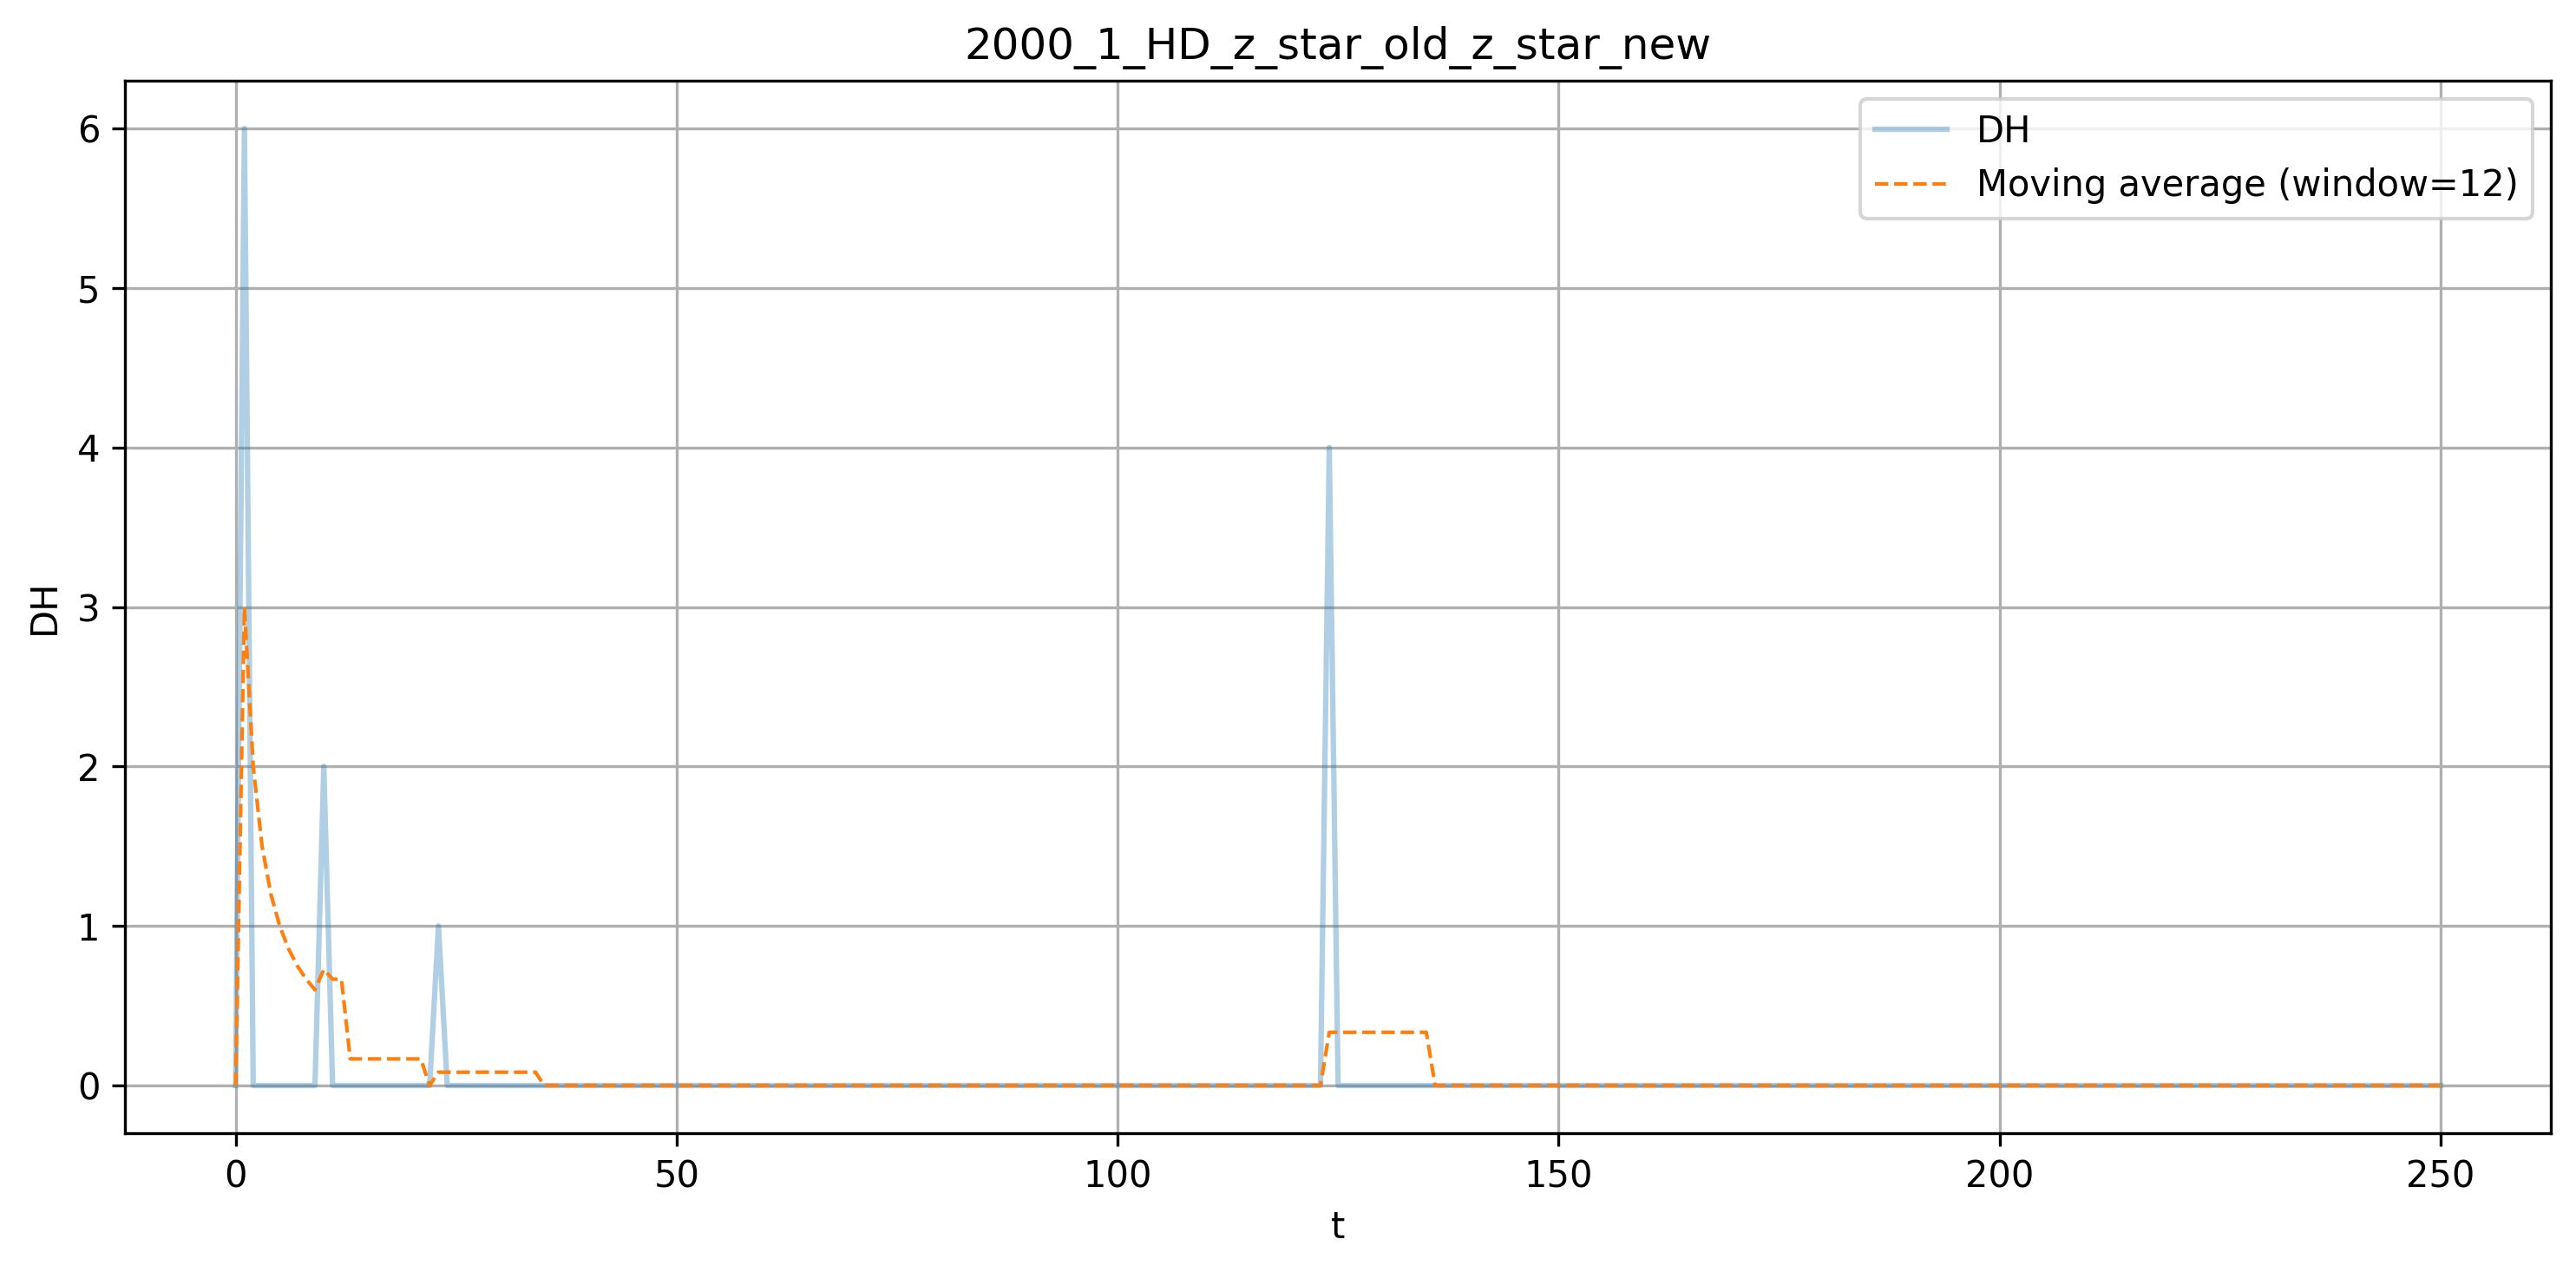
\includegraphics[width=\linewidth]{../Quantum-Annealing-for-solving-QUBO-Problems/test/Diagnostica_QALS/2/ksp_1/lambda_650_dot_C/2000_1_HD_z_star_old_z_star_new.png}
    \caption{\(d_H(z_\star^{old}, z_\star^{new})\) con \(\lambda_1\)}
    \label{fig:hd-zstarold-zstarnew-lambda1}
\end{subfigure}
\hfill
\begin{subfigure}{0.495\textwidth}
    \centering
    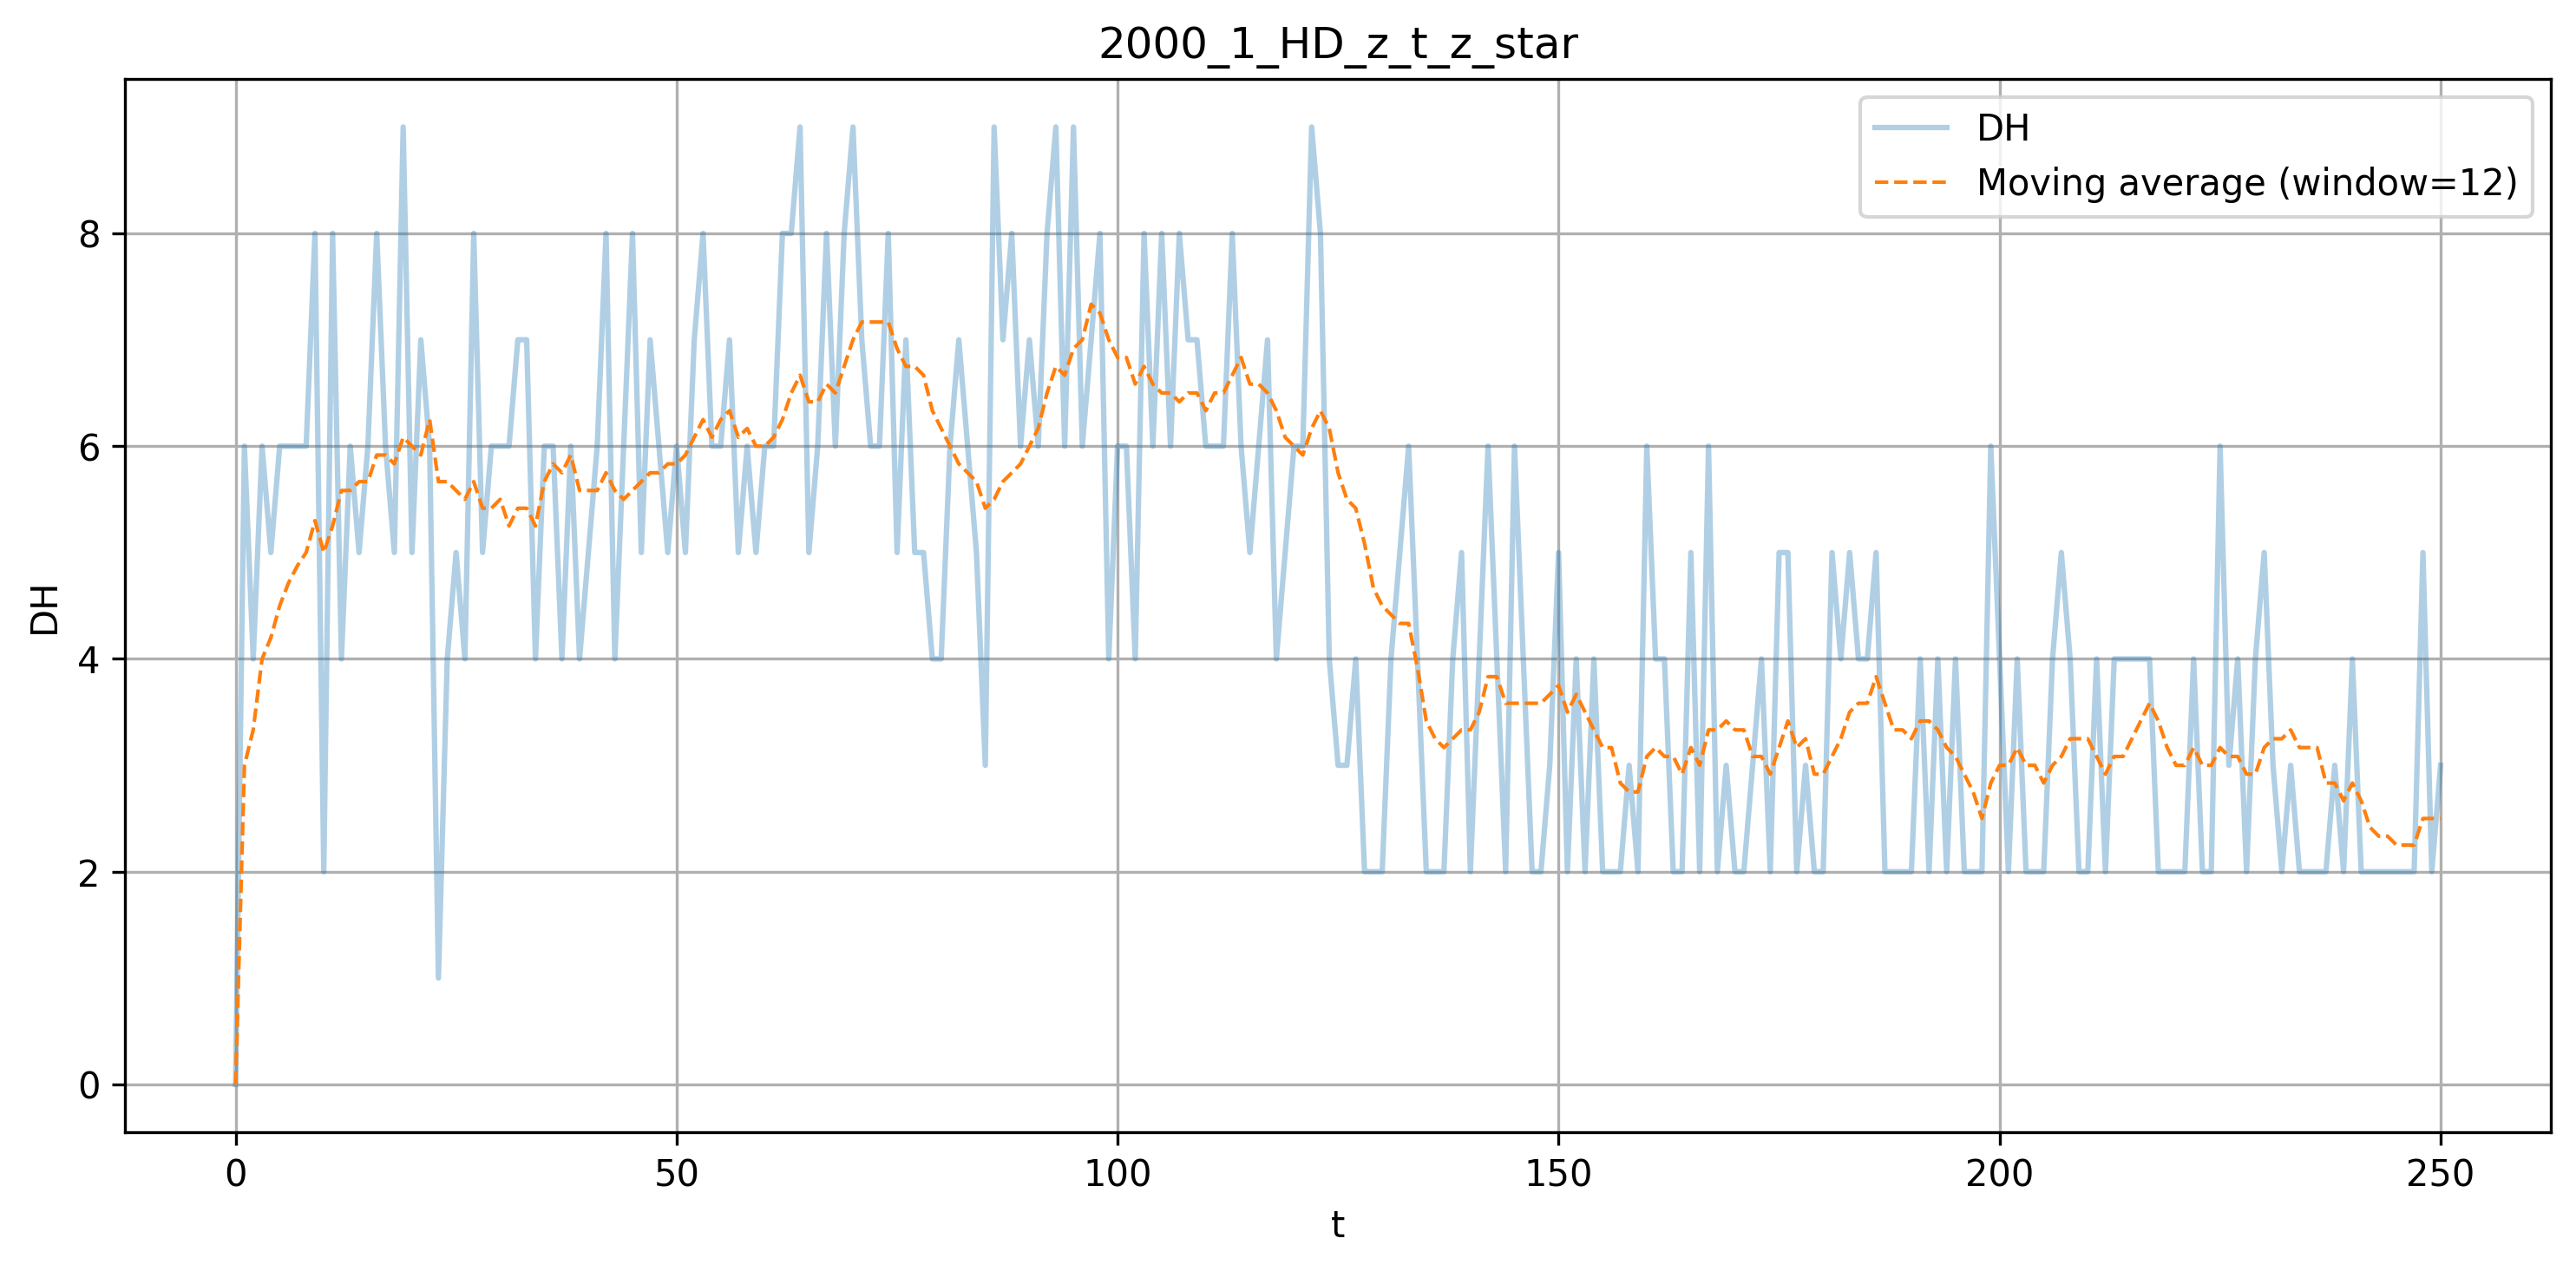
\includegraphics[width=\linewidth]{../Quantum-Annealing-for-solving-QUBO-Problems/test/Diagnostica_QALS/2/ksp_1/lambda_650_dot_C/2000_1_HD_z_t_z_star.png}
    \caption{\(d_H(z_t, z_\star)\) con \(\lambda_1\)}
    \label{fig:hd-zt-zstar-lambda1}
\end{subfigure}

\vspace{0.35cm}

\begin{subfigure}{0.495\textwidth}
    \centering
    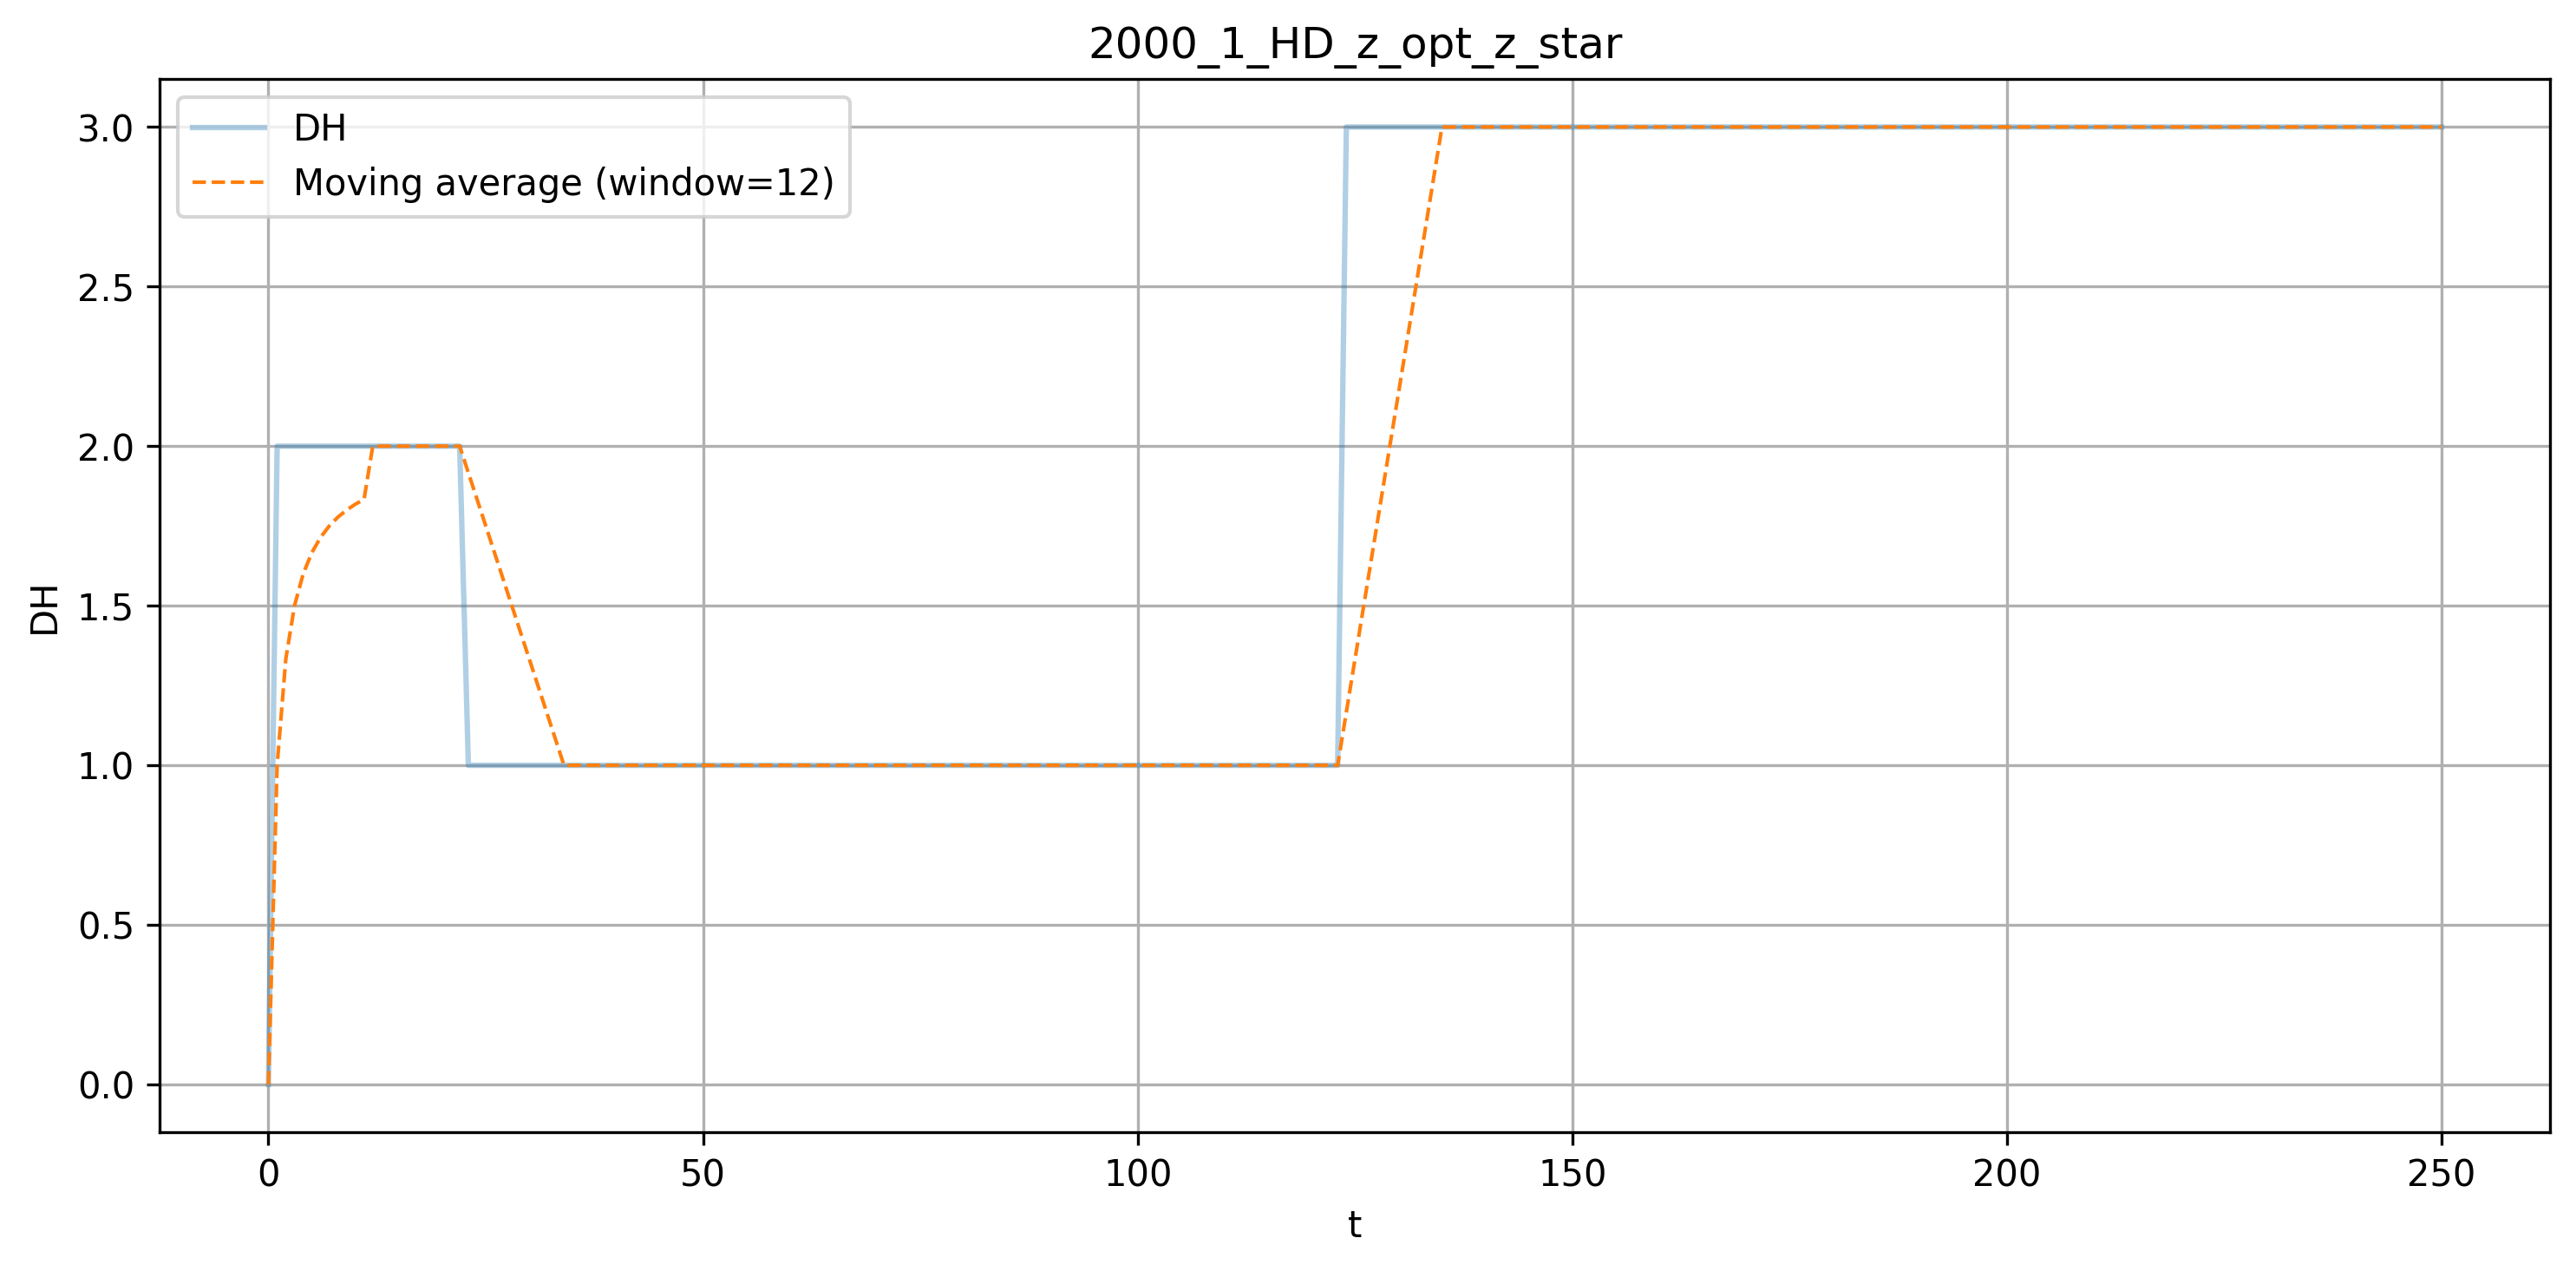
\includegraphics[width=\linewidth]{../Quantum-Annealing-for-solving-QUBO-Problems/test/Diagnostica_QALS/2/ksp_1/lambda_650_dot_C/2000_1_HD_z_opt_z_star.png}
    \caption{\(d_H(z_{opt}, z_\star)\) con \(\lambda_1\)}
    \label{fig:hd-zopt-zstar-lambda1}
\end{subfigure}
\hfill
\begin{subfigure}{0.495\textwidth}
    \centering
    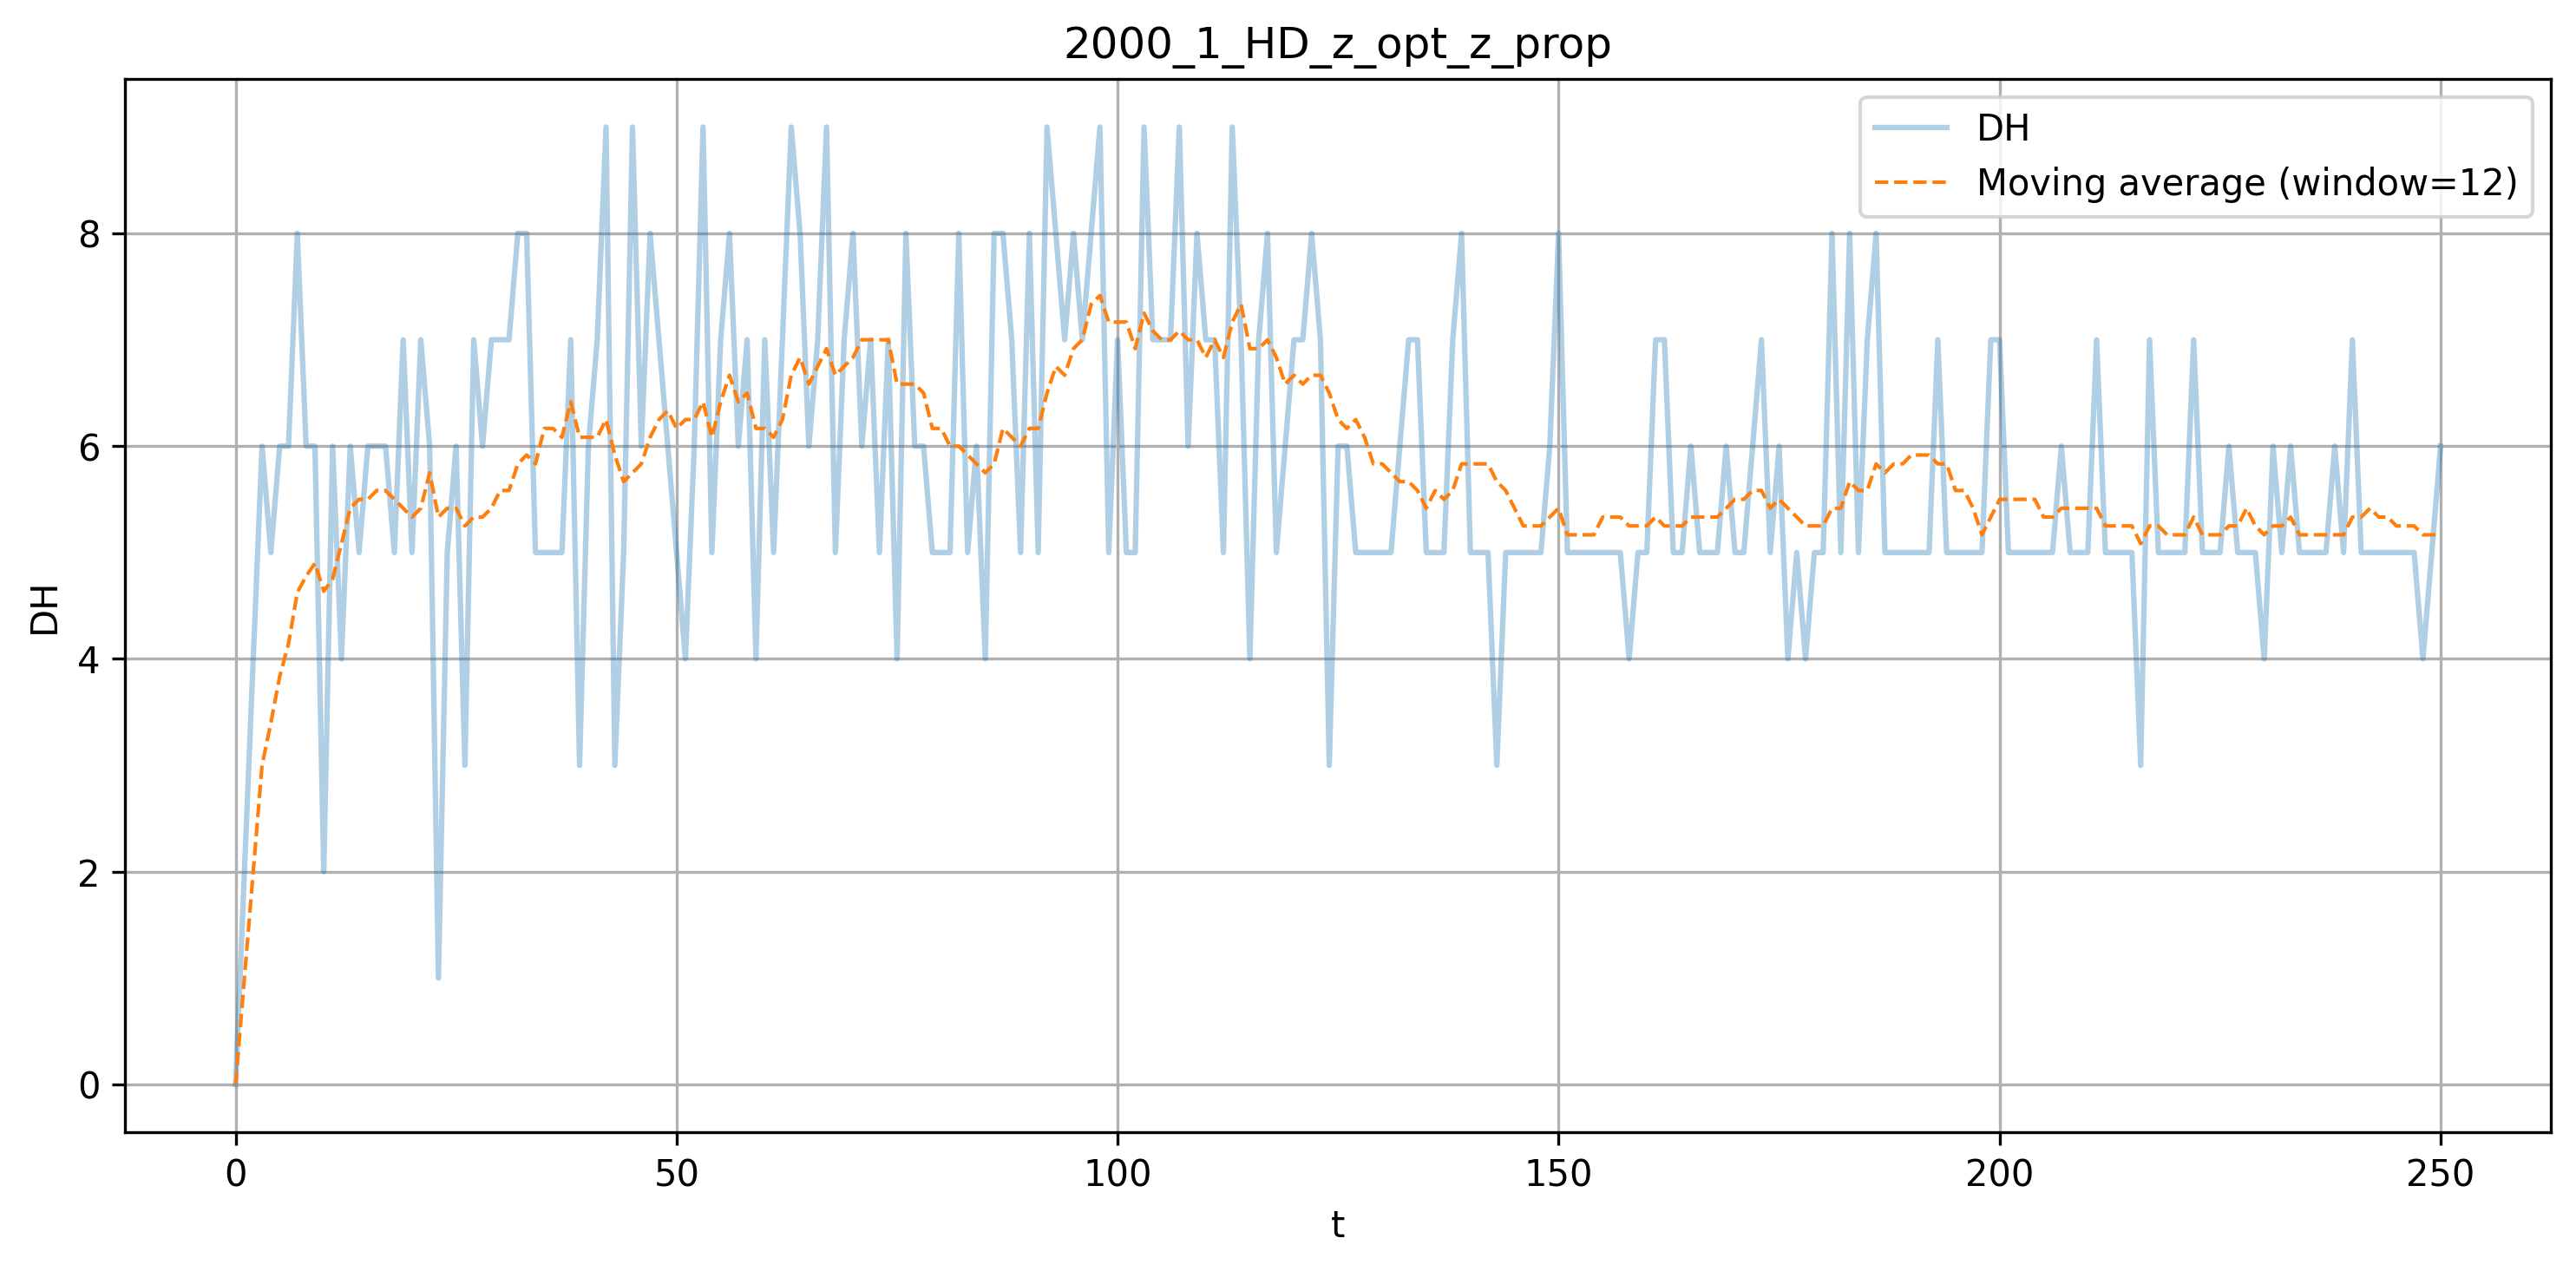
\includegraphics[width=\linewidth]{../Quantum-Annealing-for-solving-QUBO-Problems/test/Diagnostica_QALS/2/ksp_1/lambda_650_dot_C/2000_1_HD_z_opt_z_prop.png}
    \caption{\(d_H(z_{opt}, z_t)\) con \(\lambda_1\)}
    \label{fig:hd-zopt-zprop-lambda1}
\end{subfigure}

\vspace{0.35cm}

\begin{subfigure}{0.495\textwidth}
    \centering
    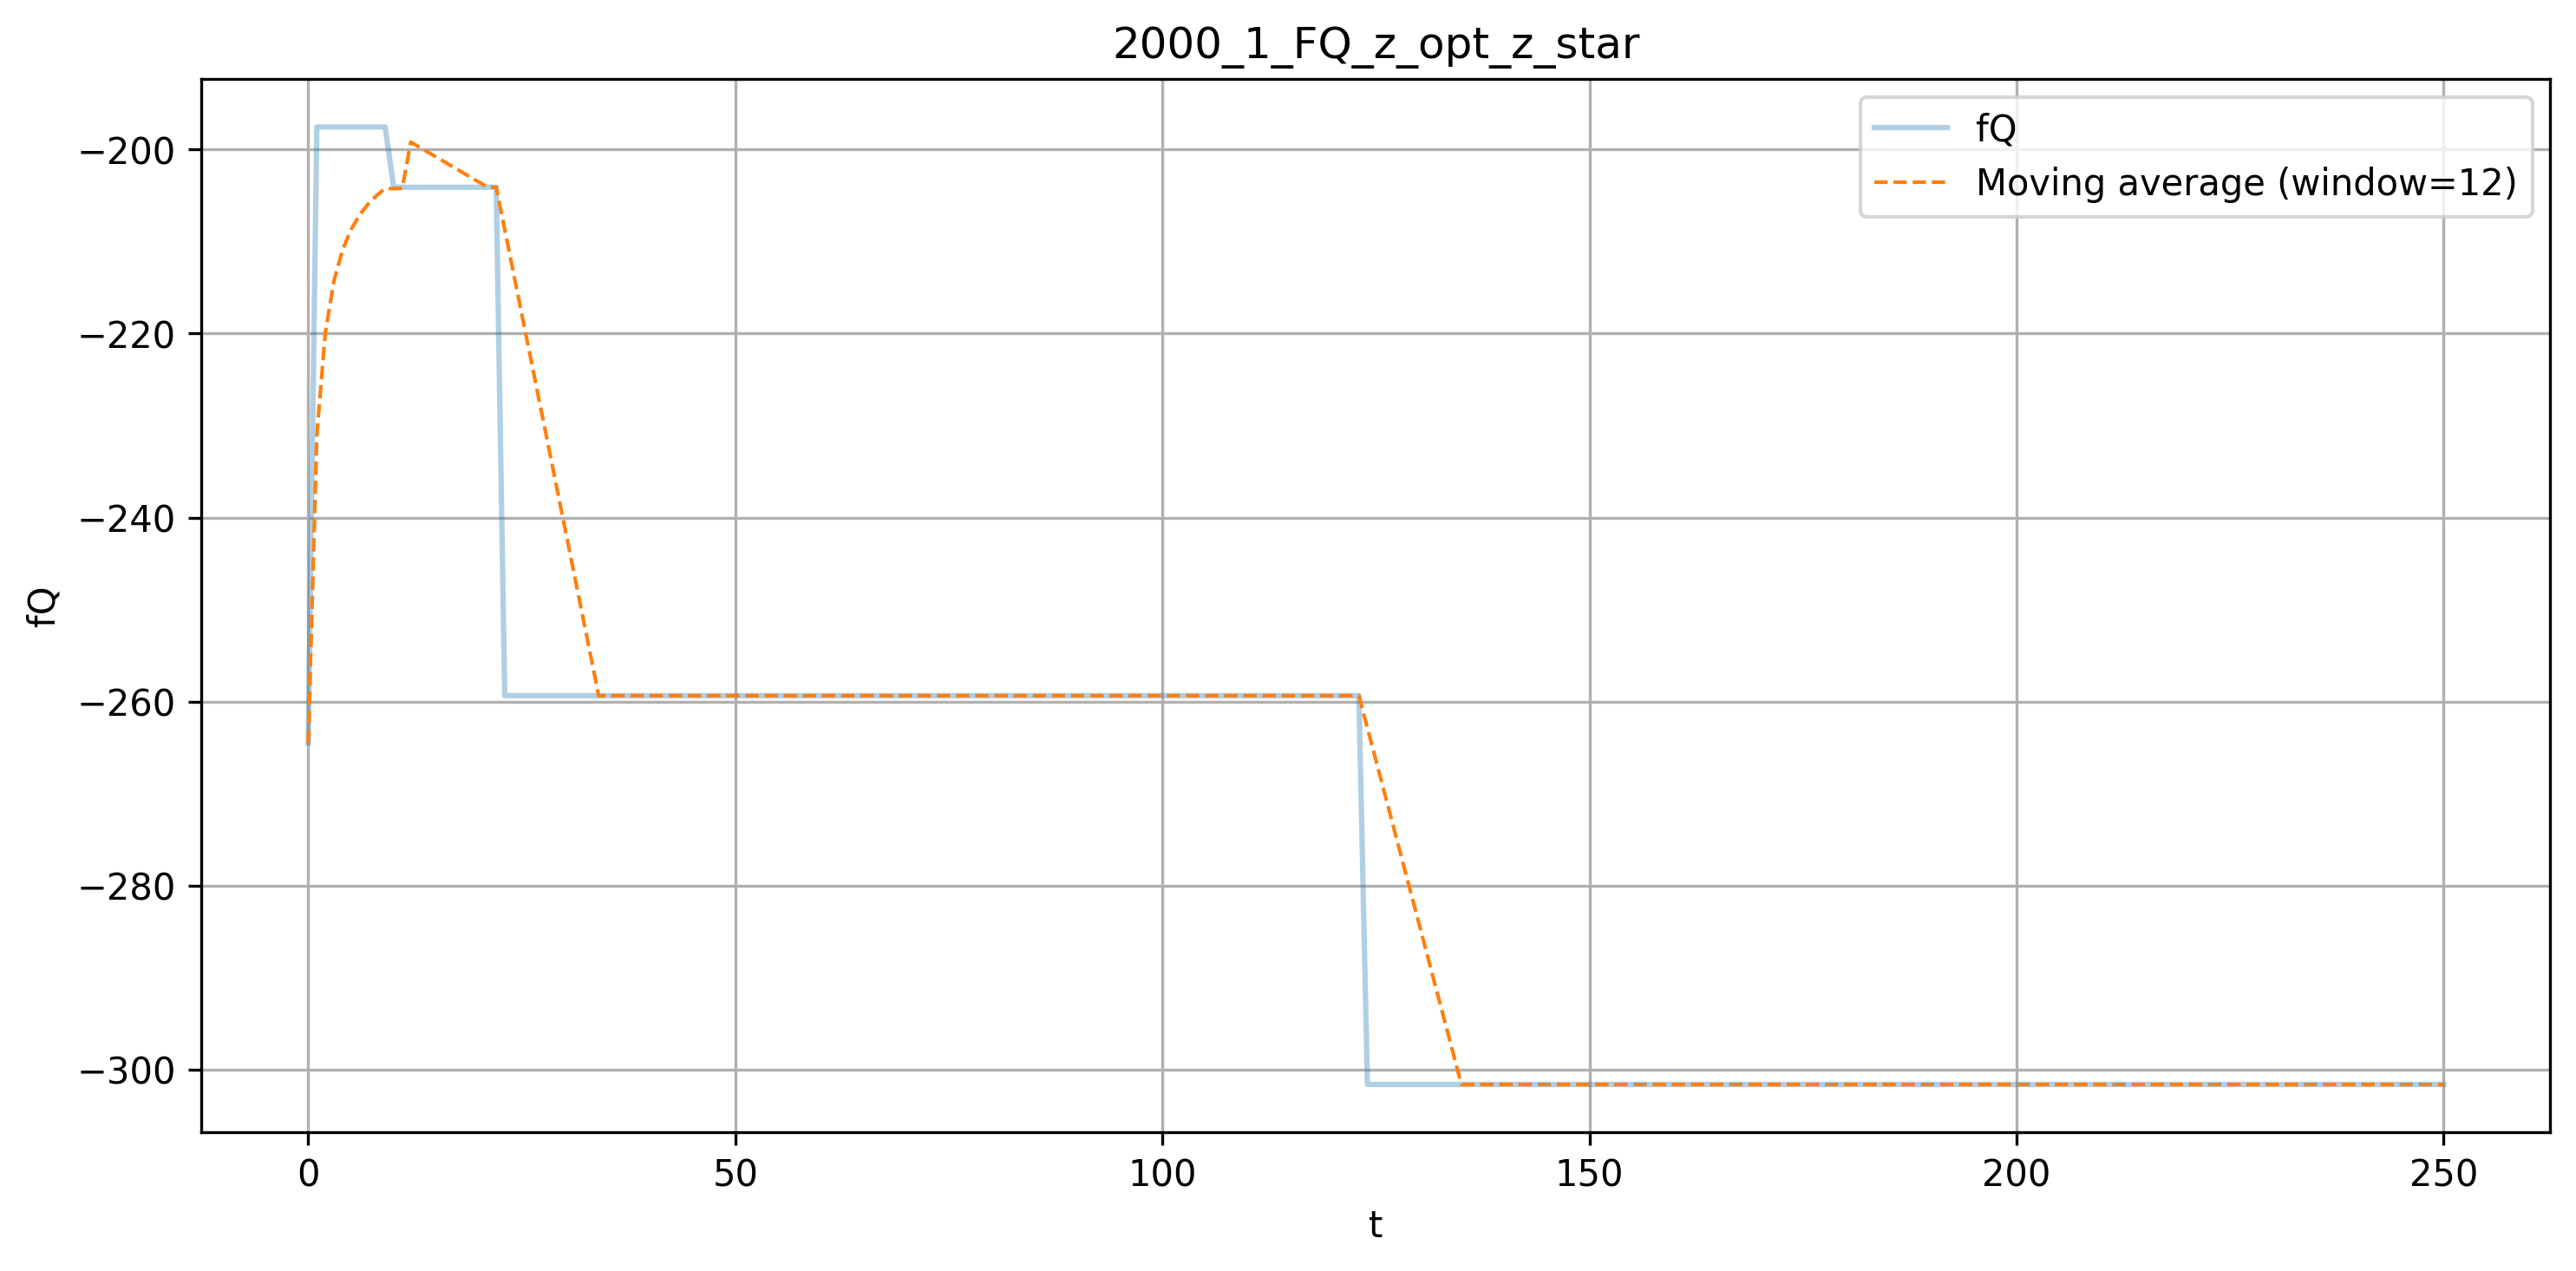
\includegraphics[width=\linewidth]{../Quantum-Annealing-for-solving-QUBO-Problems/test/Diagnostica_QALS/2/ksp_1/lambda_650_dot_C/2000_1_FQ_z_opt_z_star.png}
    \caption{\(f_Q(z_\star)\) con \(\lambda_1\)}
    \label{fig:fQ-zstar-lambda1}
\end{subfigure}
\hfill
\begin{subfigure}{0.495\textwidth}
    \centering
    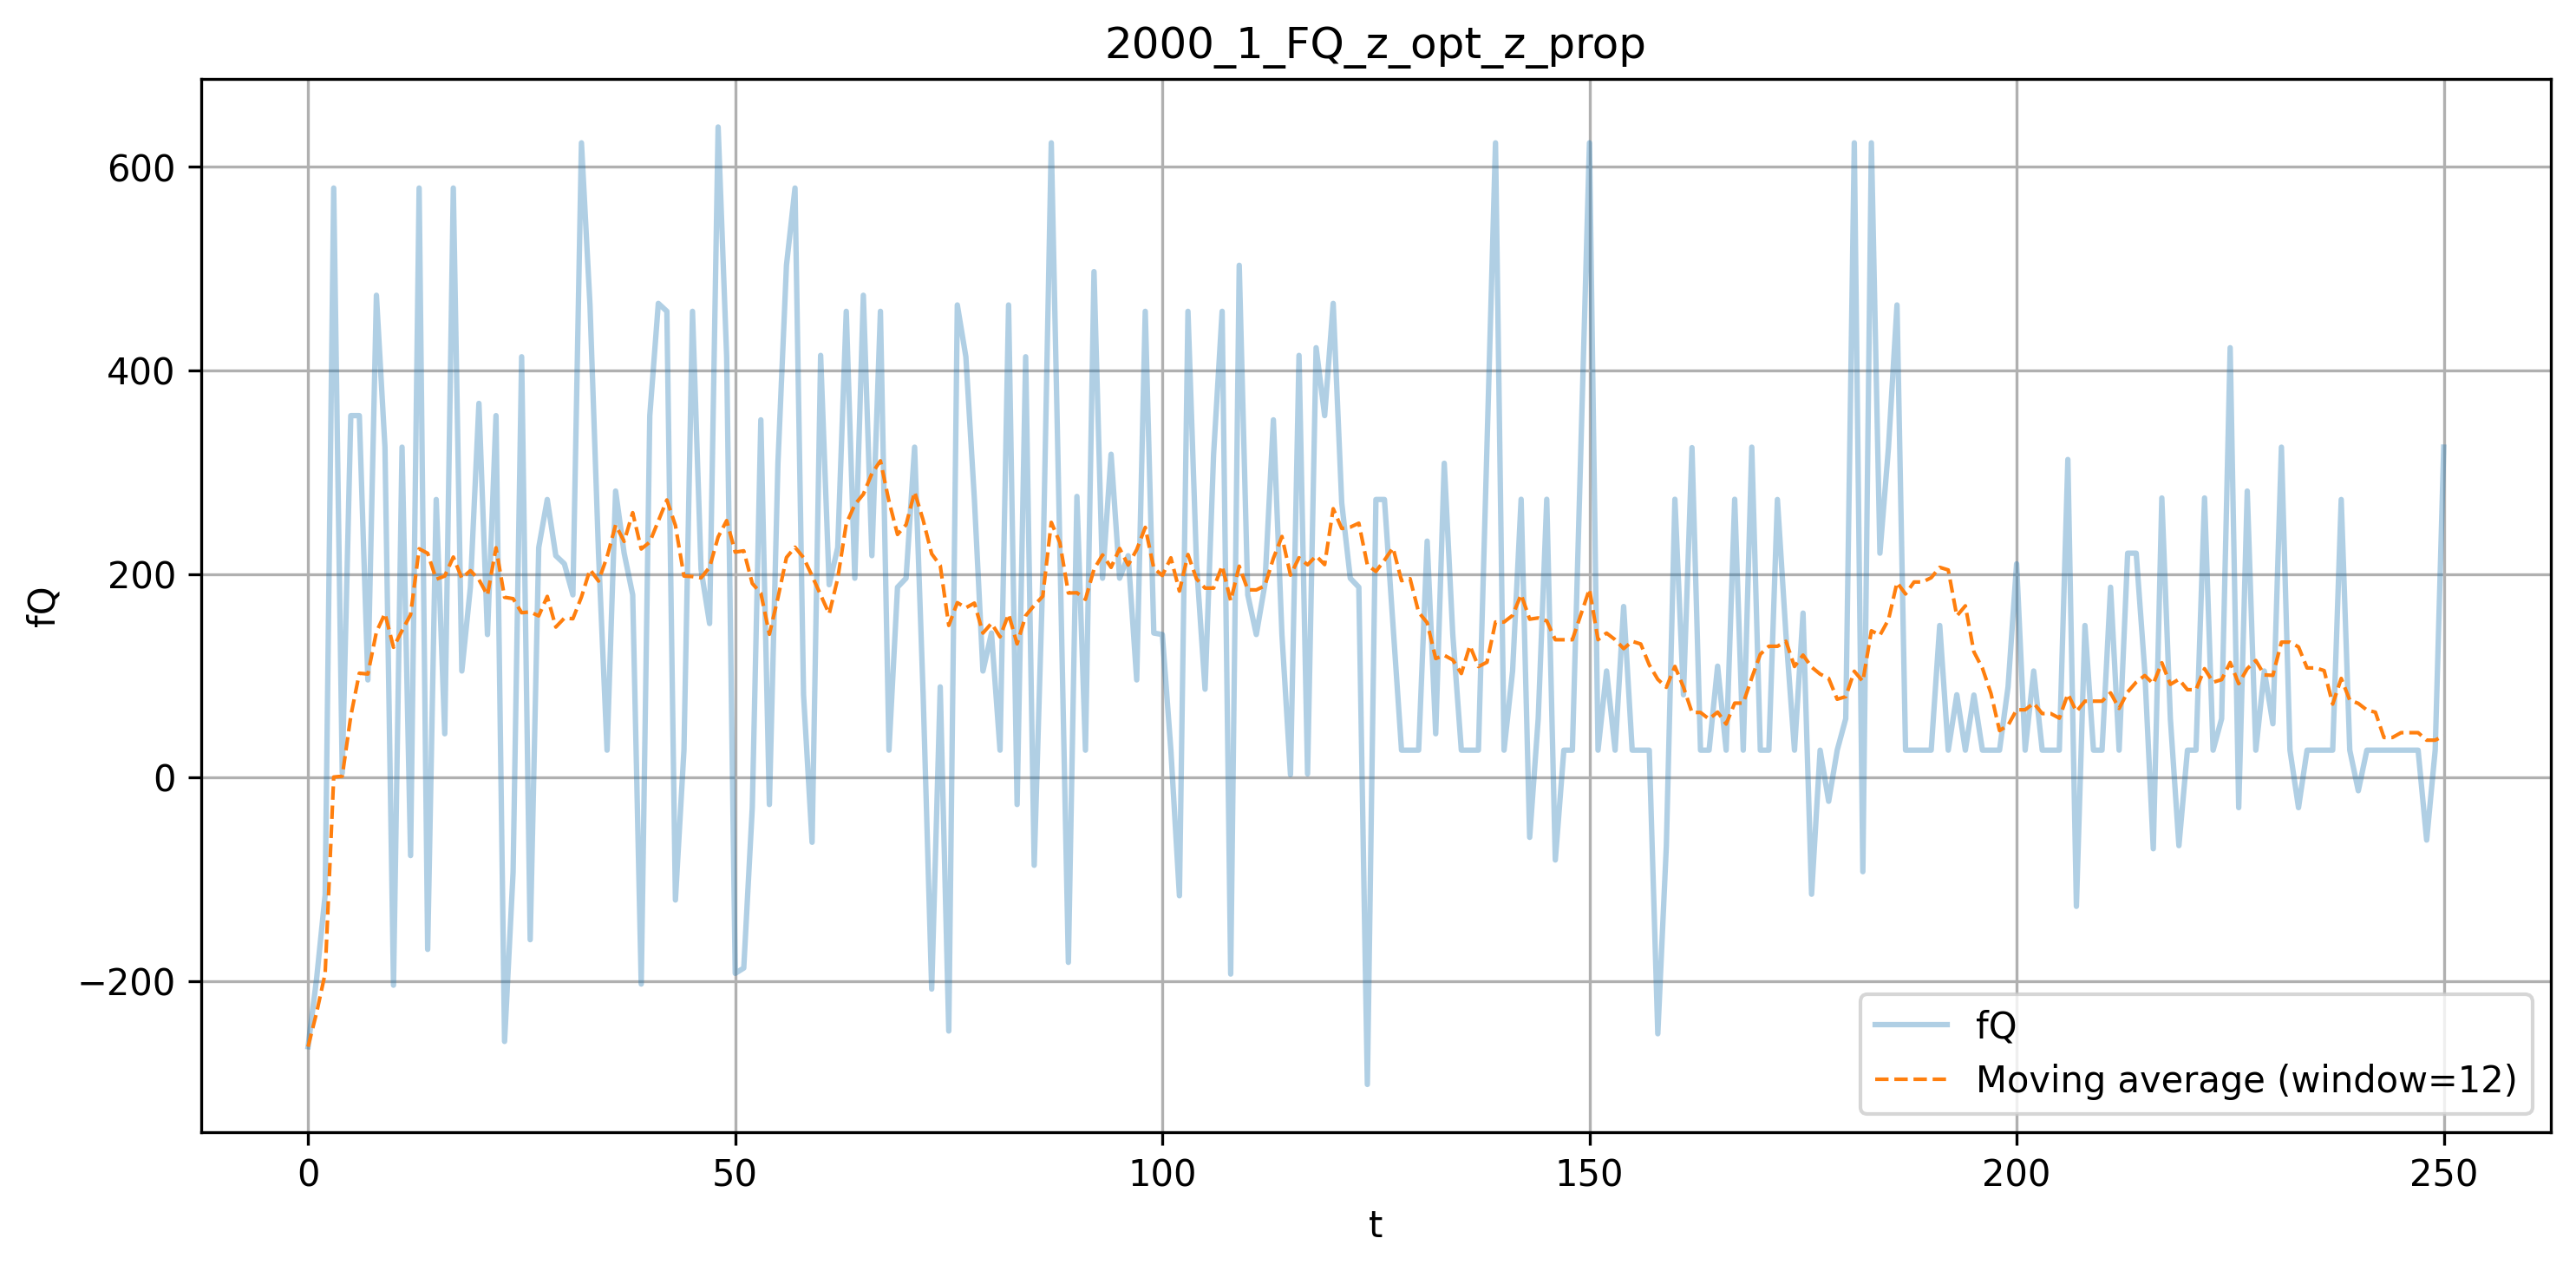
\includegraphics[width=\linewidth]{../Quantum-Annealing-for-solving-QUBO-Problems/test/Diagnostica_QALS/2/ksp_1/lambda_650_dot_C/2000_1_FQ_z_opt_z_prop.png}
    \caption{\(f_Q(z_t)\) con \(\lambda_1\)}
    \label{fig:fQ-zt-lambda1}
\end{subfigure}
\label{fig:confronto-hamming-ksp11}
\end{figure}

\begin{figure}[H]
\centering
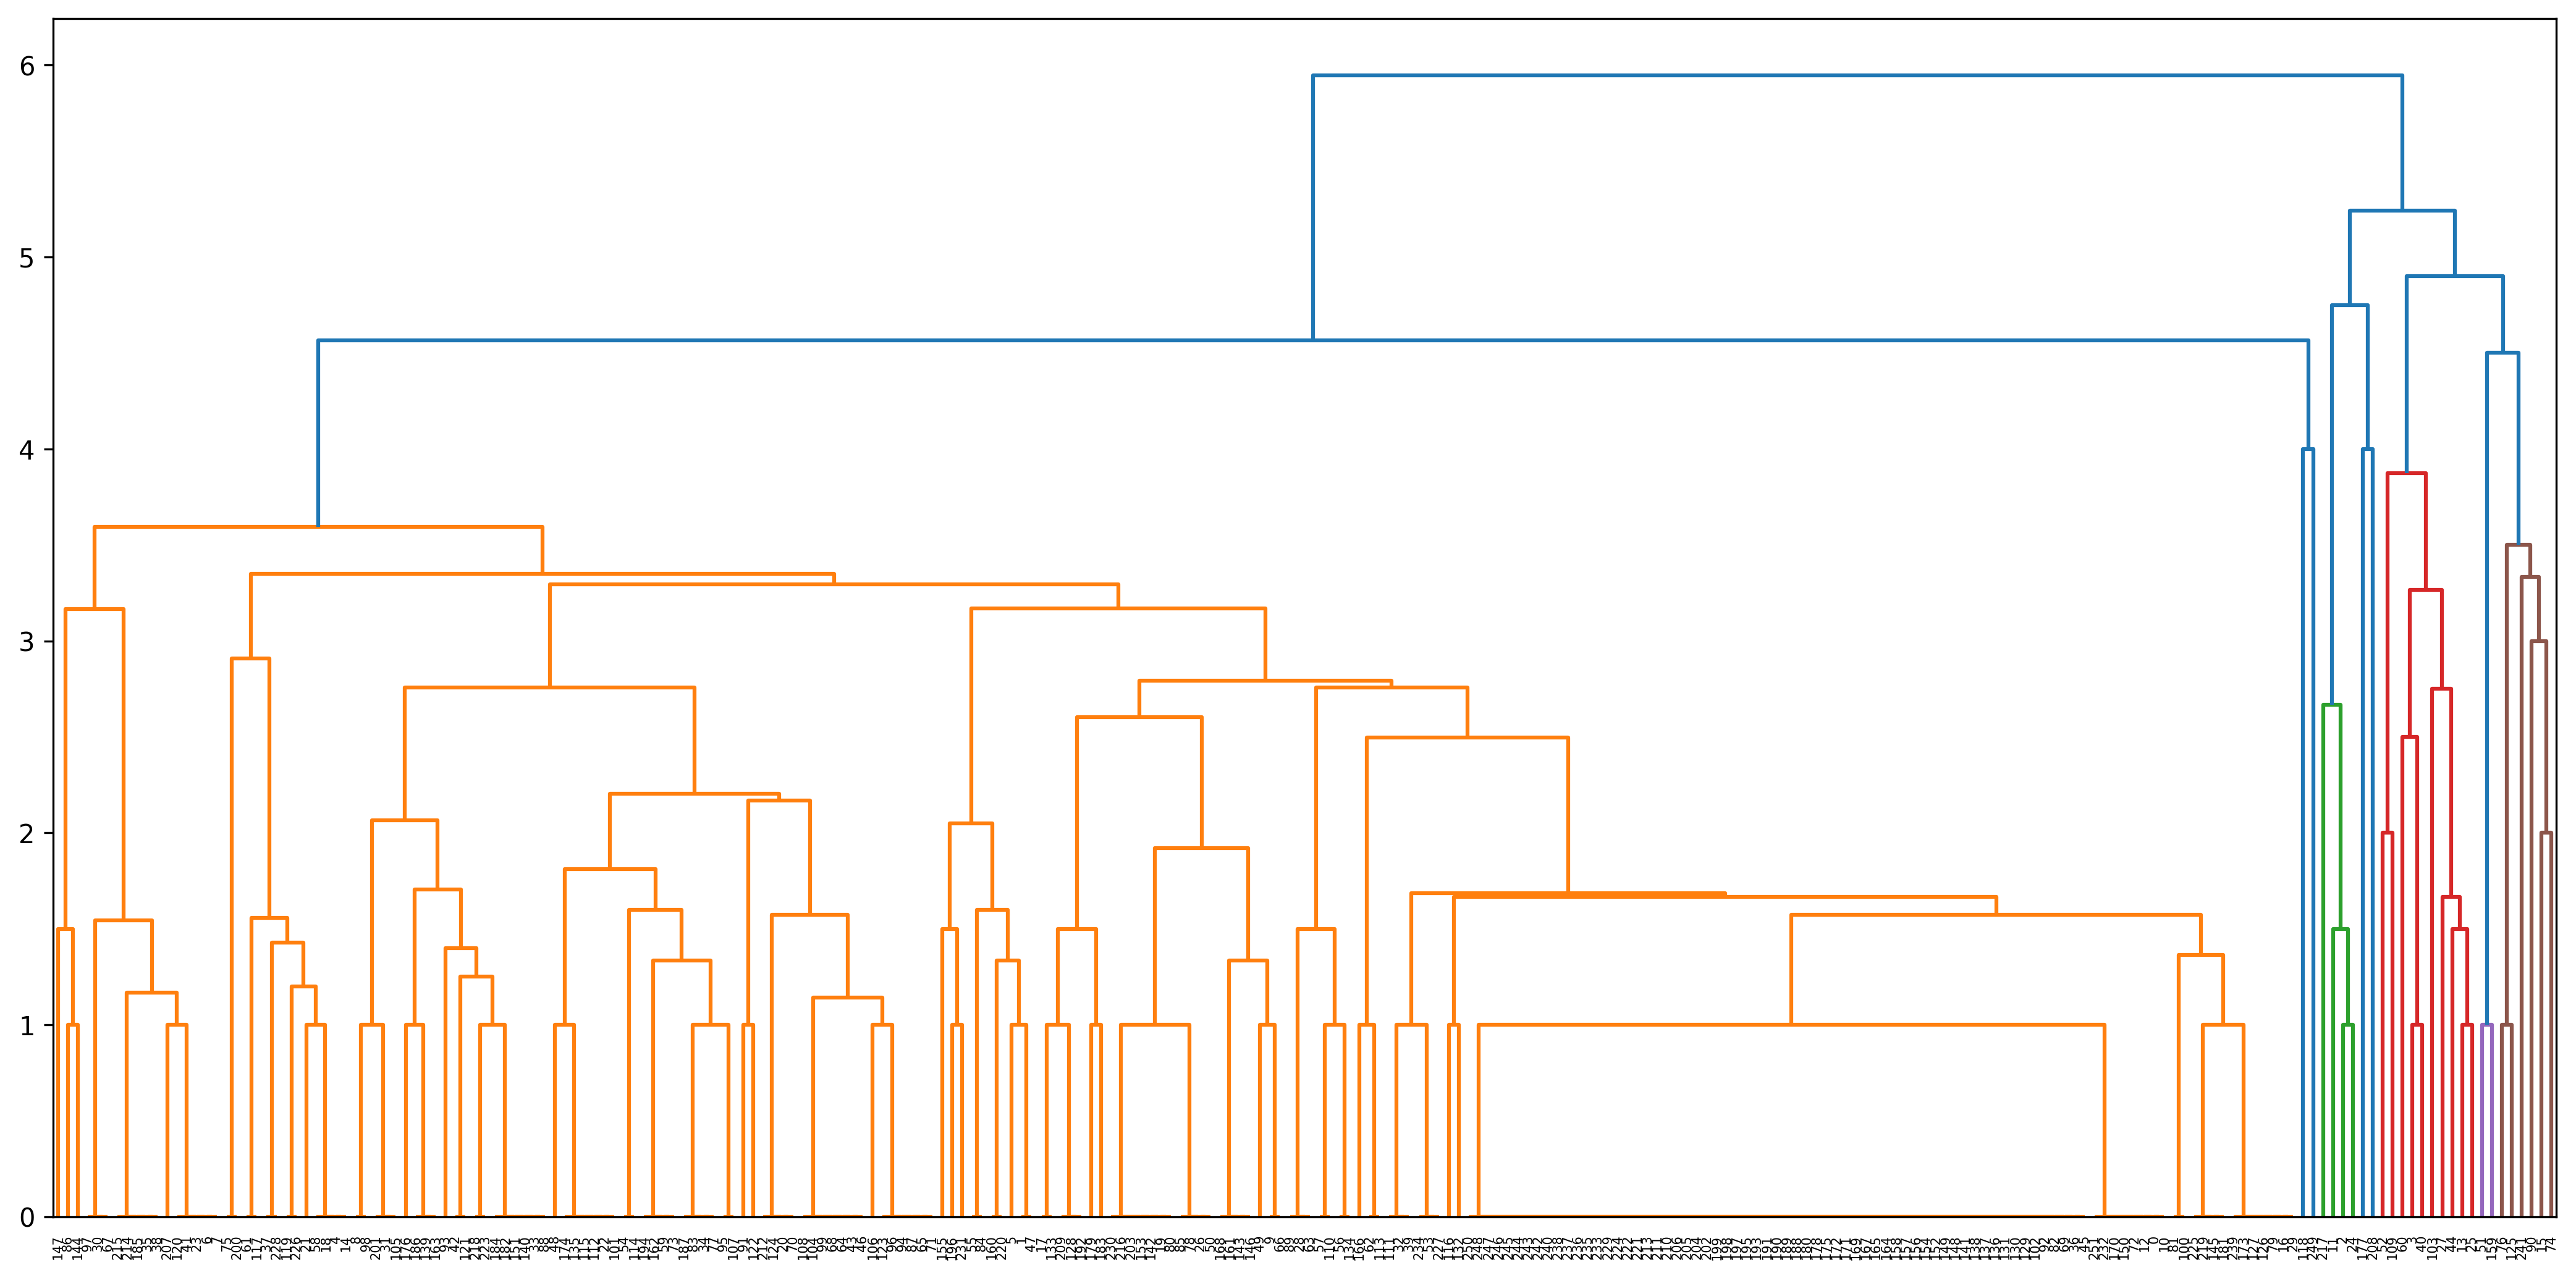
\includegraphics[width=\linewidth]{../Quantum-Annealing-for-solving-QUBO-Problems/test/Diagnostica_QALS/2/ksp_1/lambda_650_dot_C/dendrogram_2000_1.png}
\caption{Agglomerative Clustering Dendogram}
\label{fig:AgglomerativeClustering-ksp1}
\end{figure}
\clearpage

\begin{figure}[H]
\centering
\begin{subfigure}{0.495\textwidth}
    \centering
    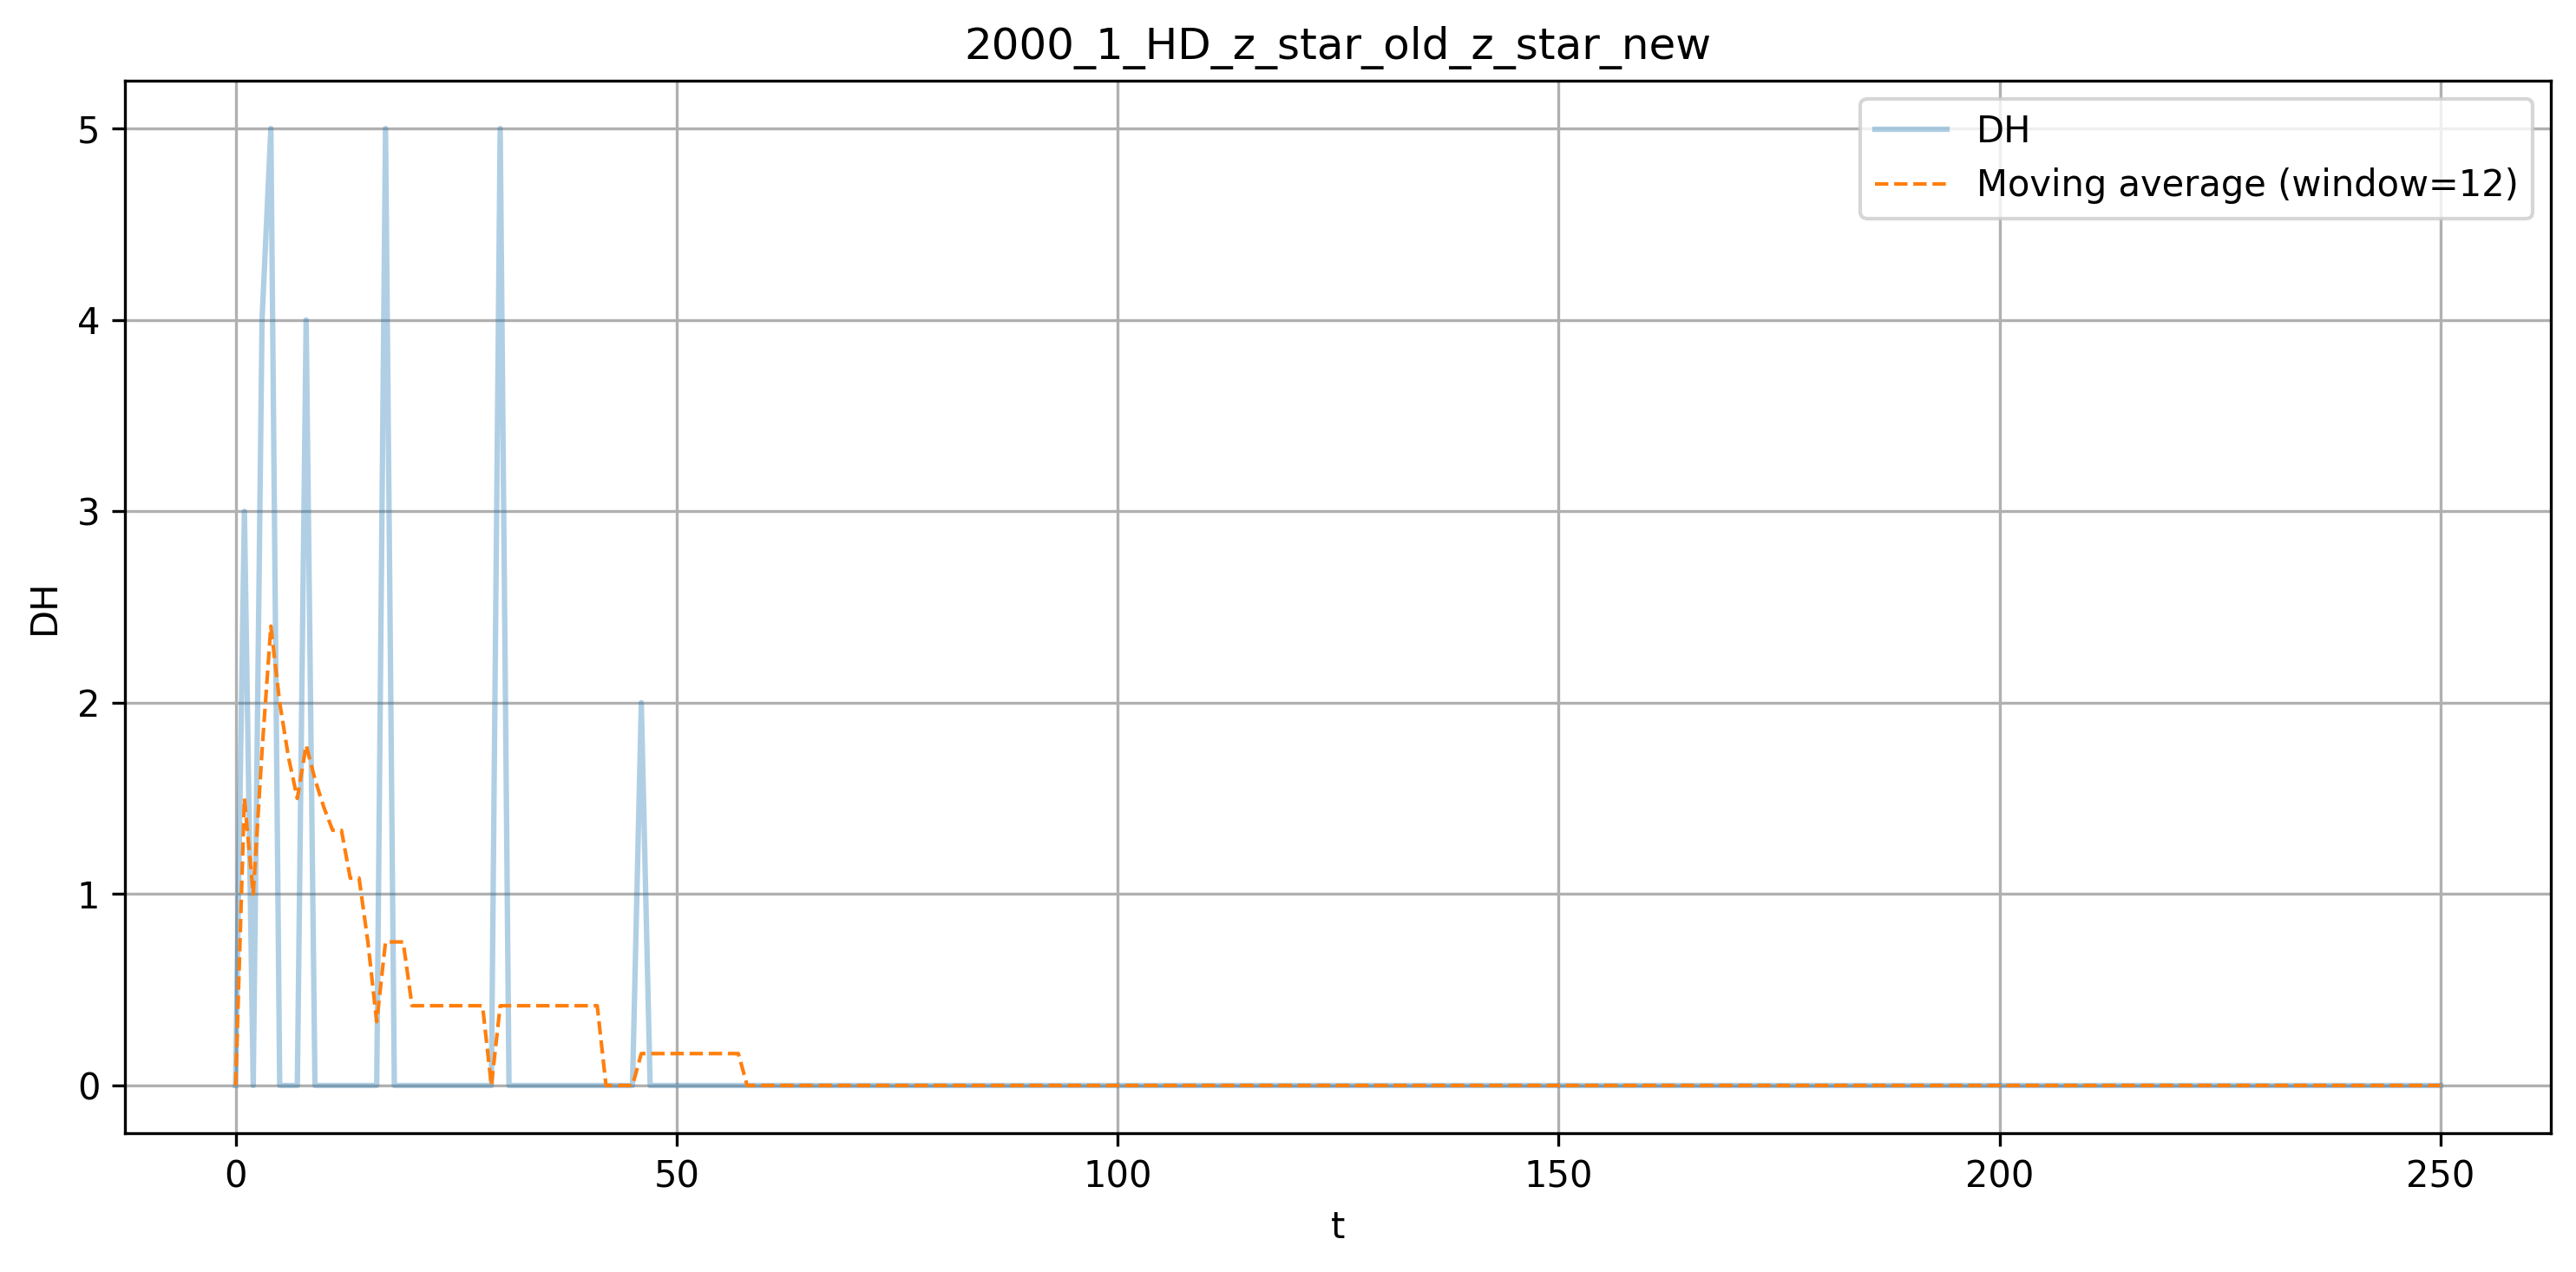
\includegraphics[width=\linewidth]{../Quantum-Annealing-for-solving-QUBO-Problems/test/Diagnostica_QALS/2/ksp_1/lambda_div_3/2000_1_HD_z_star_old_z_star_new.png}
    \caption{\(d_H(z_\star^{old}, z_\star^{new})\) con \(\lambda_2\)}
    \label{fig:hd-zstarold-zstarnew-lambda2}
\end{subfigure}
\hfill
\begin{subfigure}{0.495\textwidth}
    \centering
    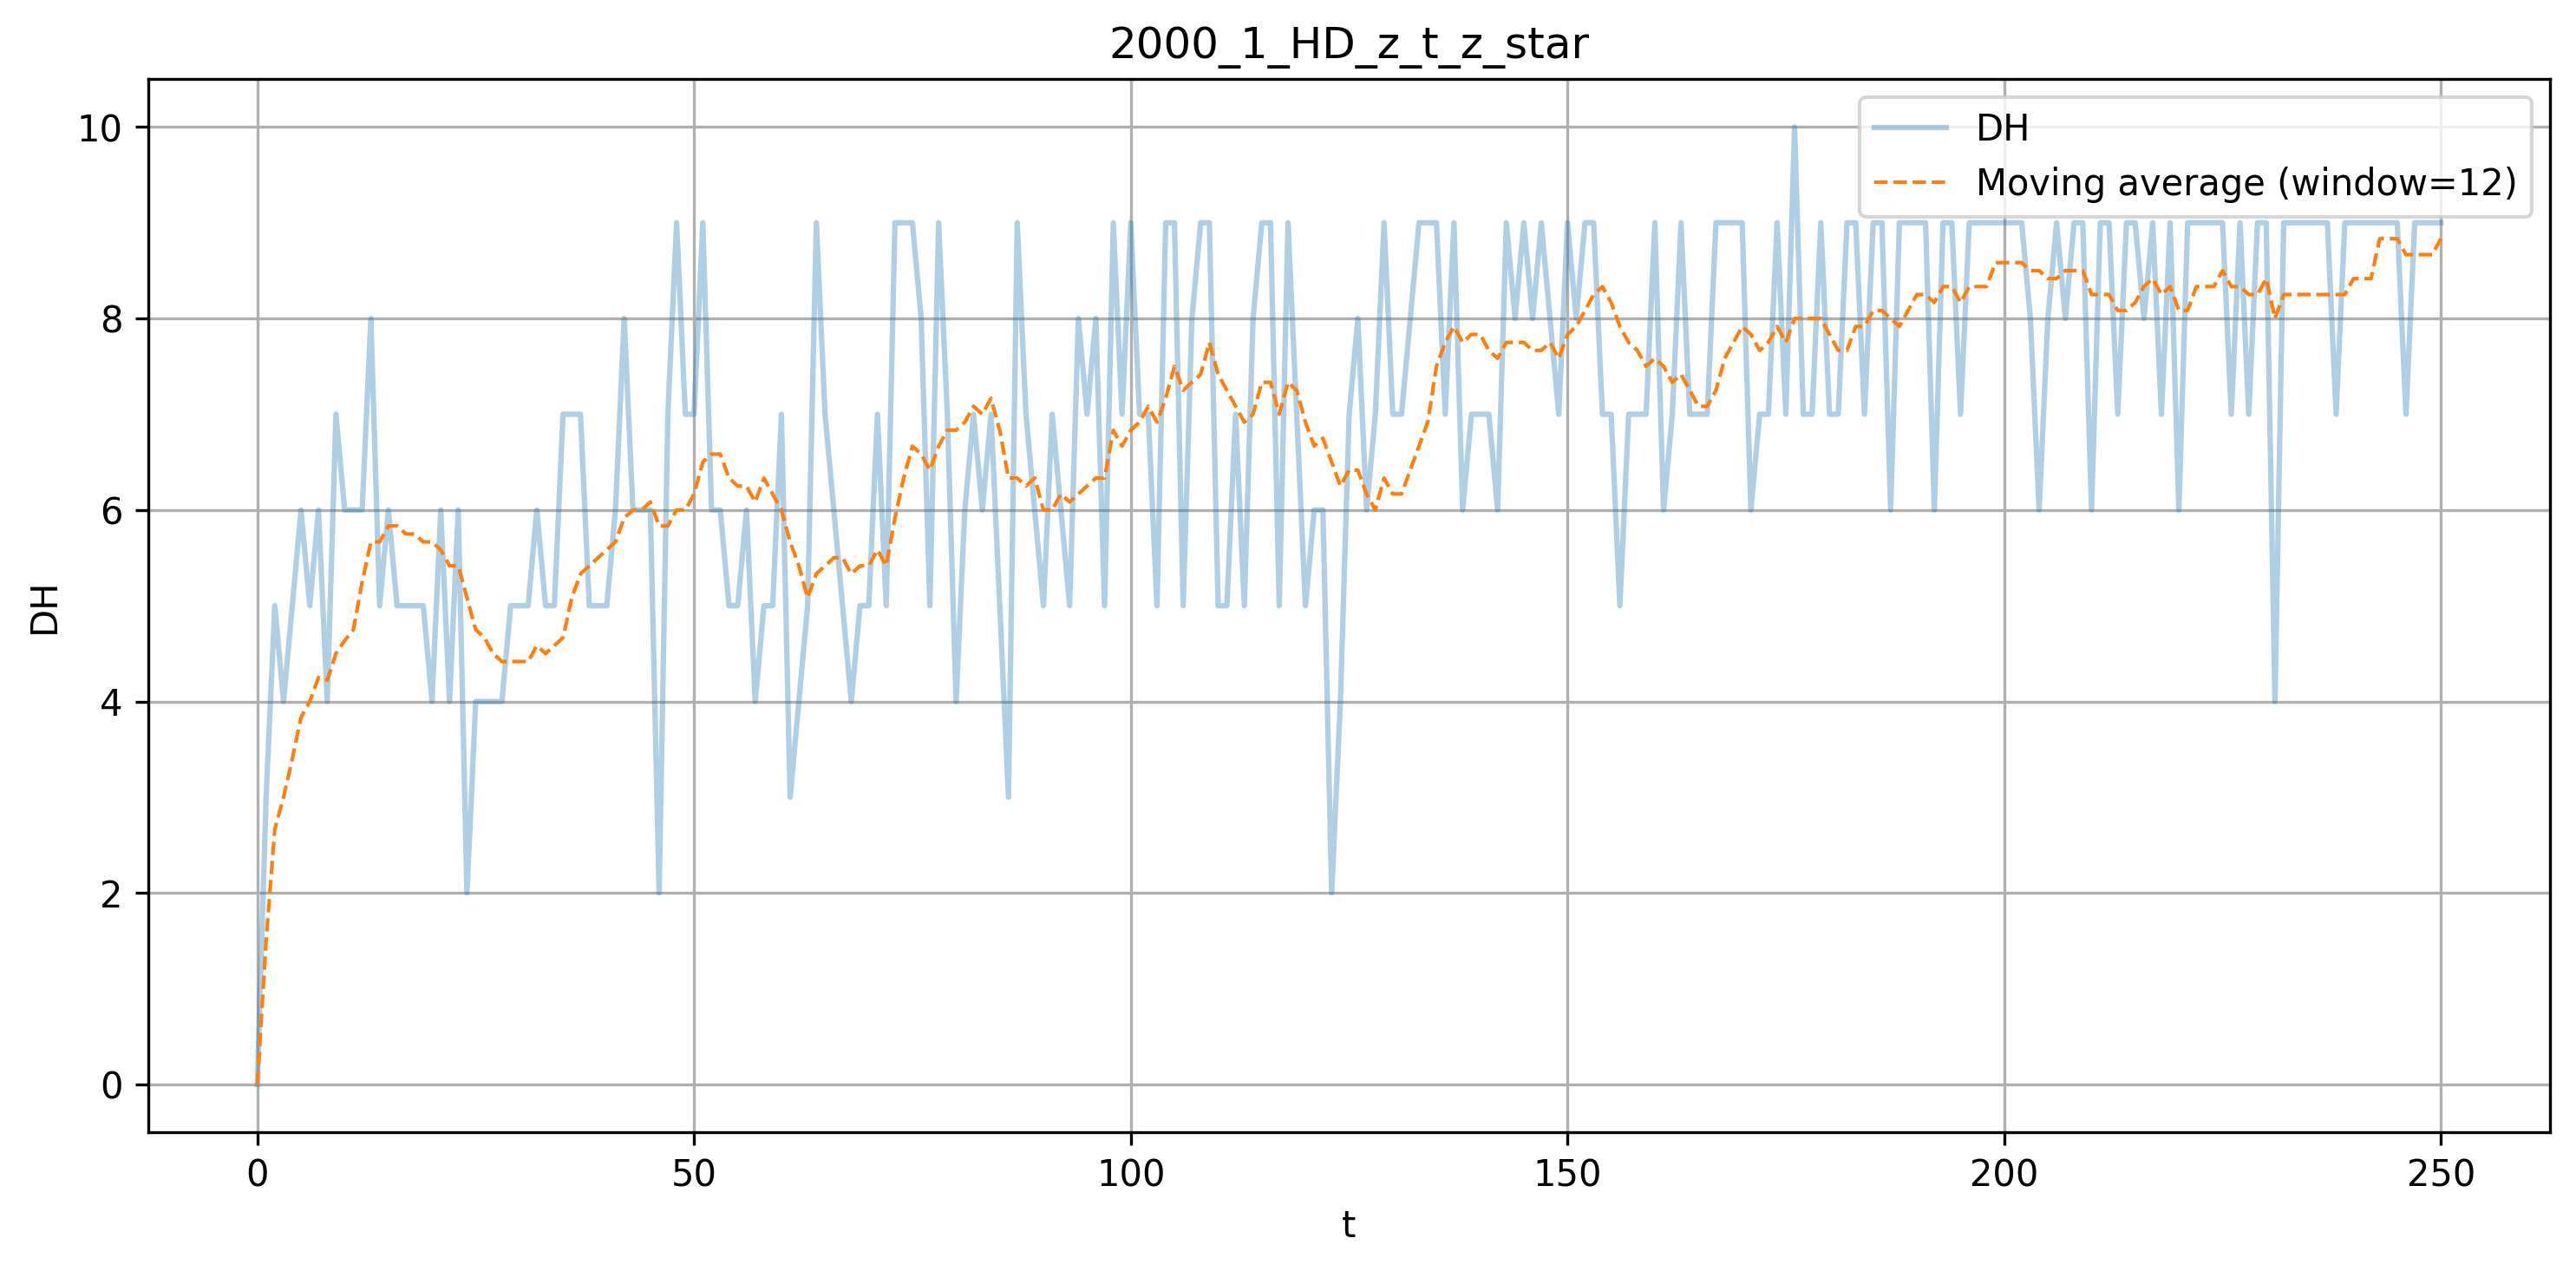
\includegraphics[width=\linewidth]{../Quantum-Annealing-for-solving-QUBO-Problems/test/Diagnostica_QALS/2/ksp_1/lambda_div_3/2000_1_HD_z_t_z_star.png}
    \caption{\(d_H(z_t, z_\star)\) con \(\lambda_2\)}
    \label{fig:hd-zt-zstar-lambda2}
\end{subfigure}

\vspace{0.35cm}

\begin{subfigure}{0.495\textwidth}
    \centering
    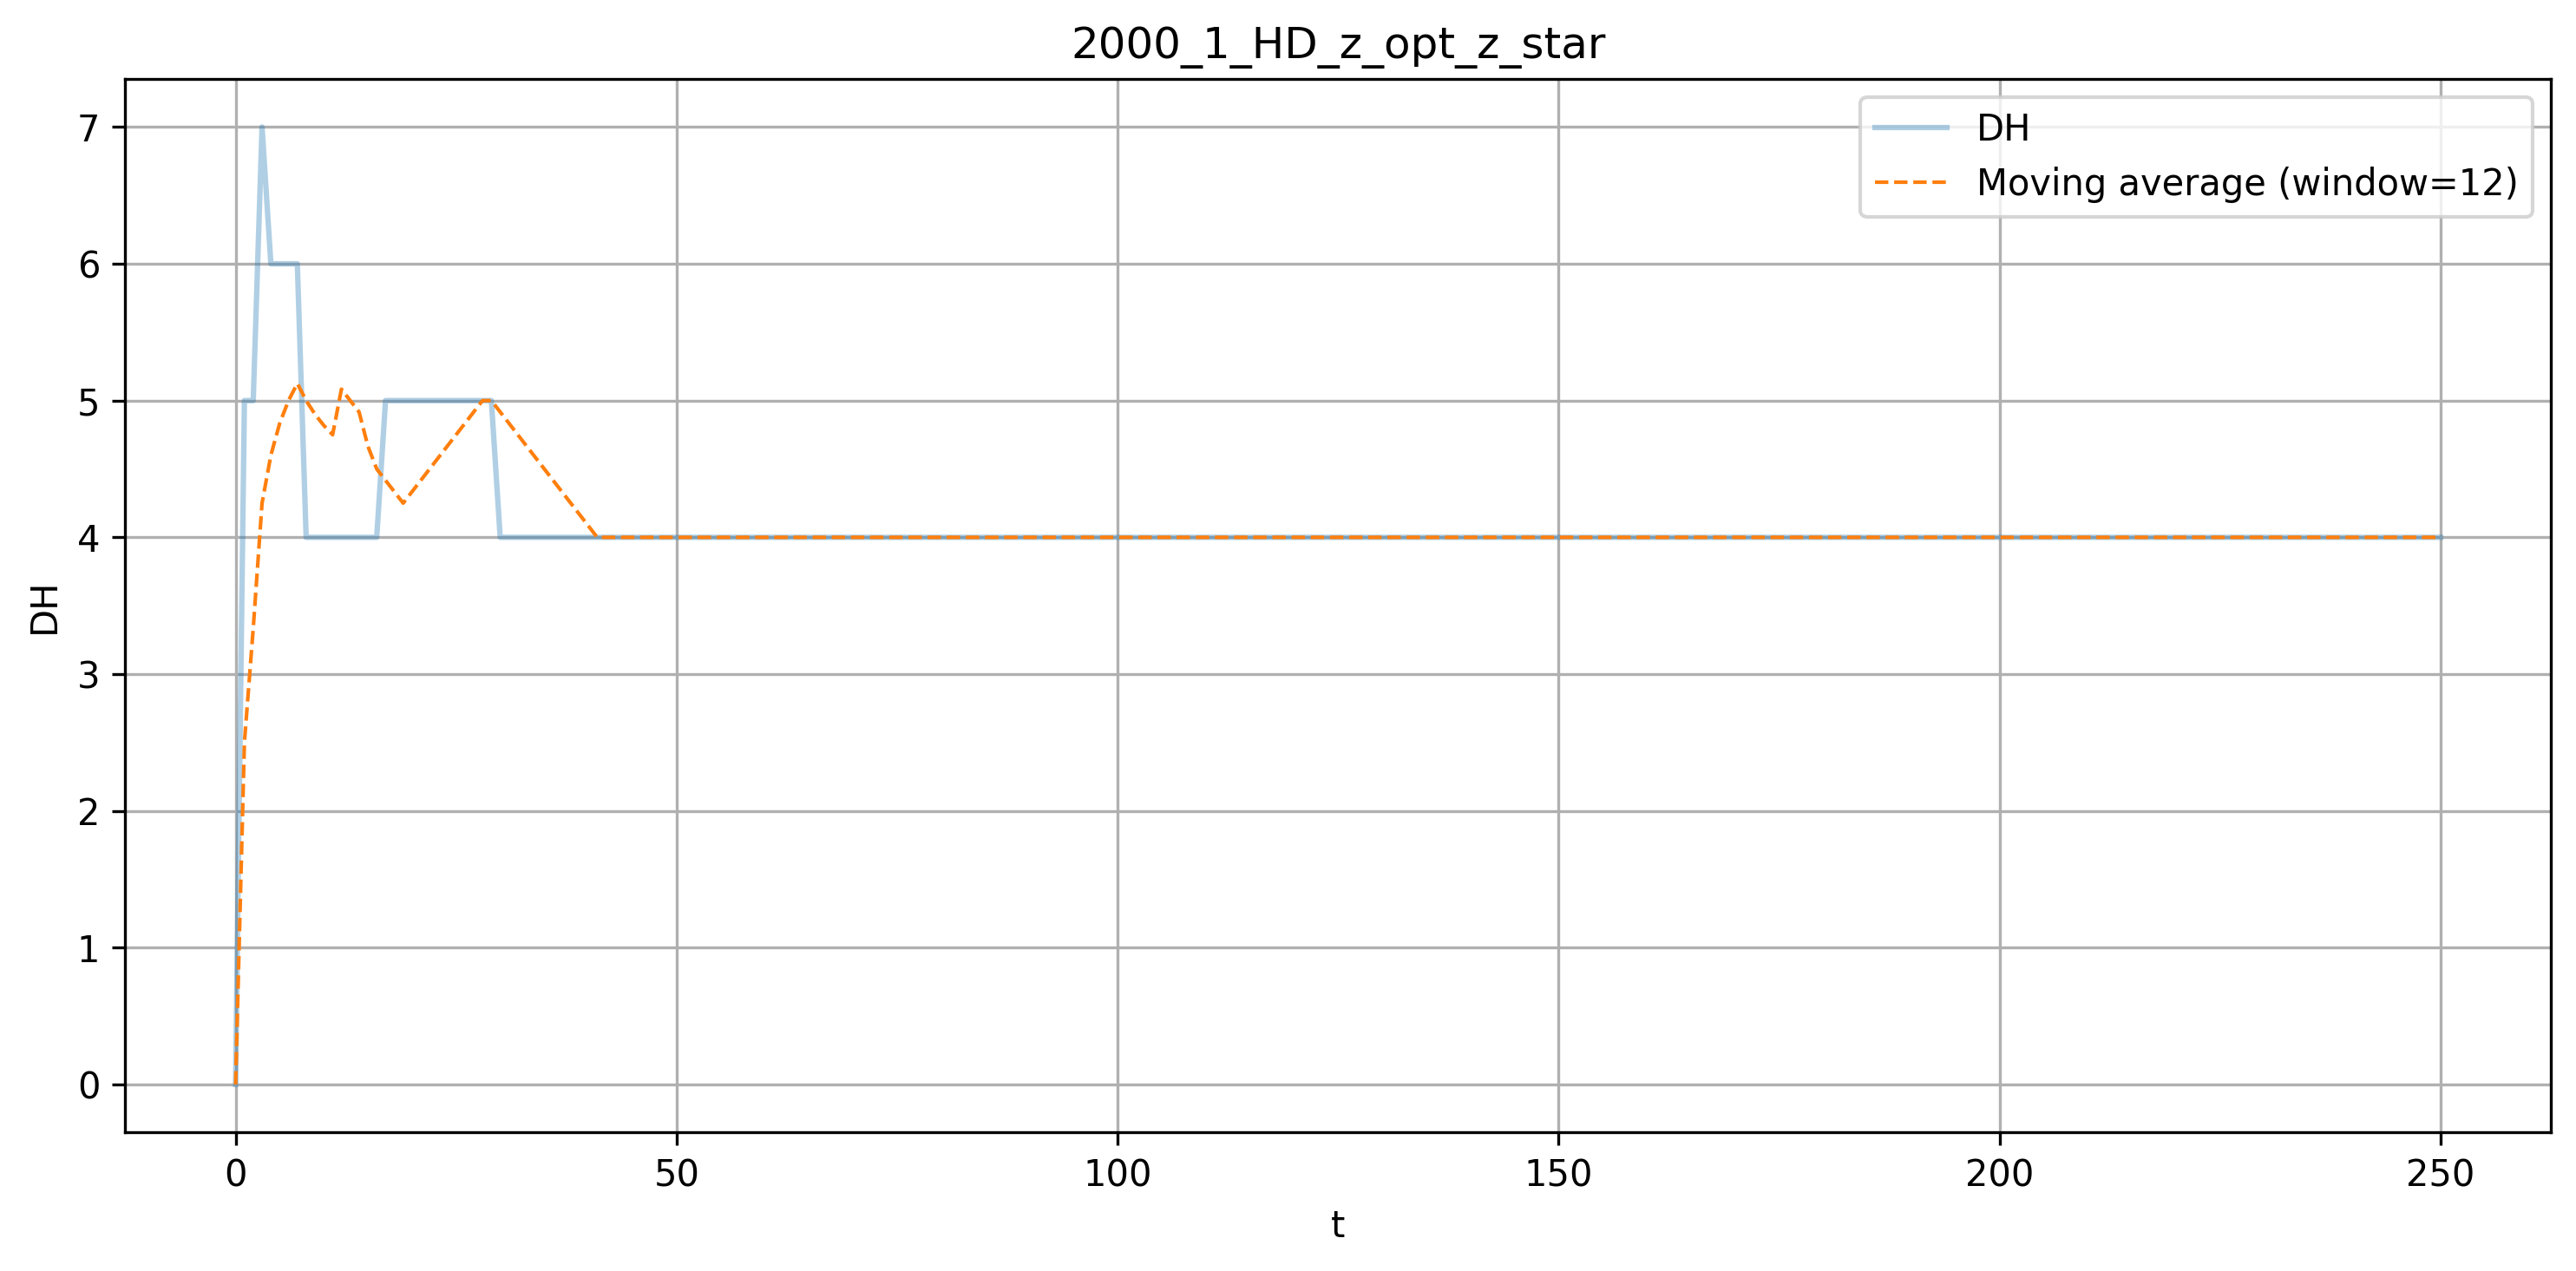
\includegraphics[width=\linewidth]{../Quantum-Annealing-for-solving-QUBO-Problems/test/Diagnostica_QALS/2/ksp_1/lambda_div_3/2000_1_HD_z_opt_z_star.png}
    \caption{\(d_H(z_{opt}, z_\star)\) con \(\lambda_2\)}
    \label{fig:hd-zopt-zstar-lambda2}
\end{subfigure}
\hfill
\begin{subfigure}{0.495\textwidth}
    \centering
    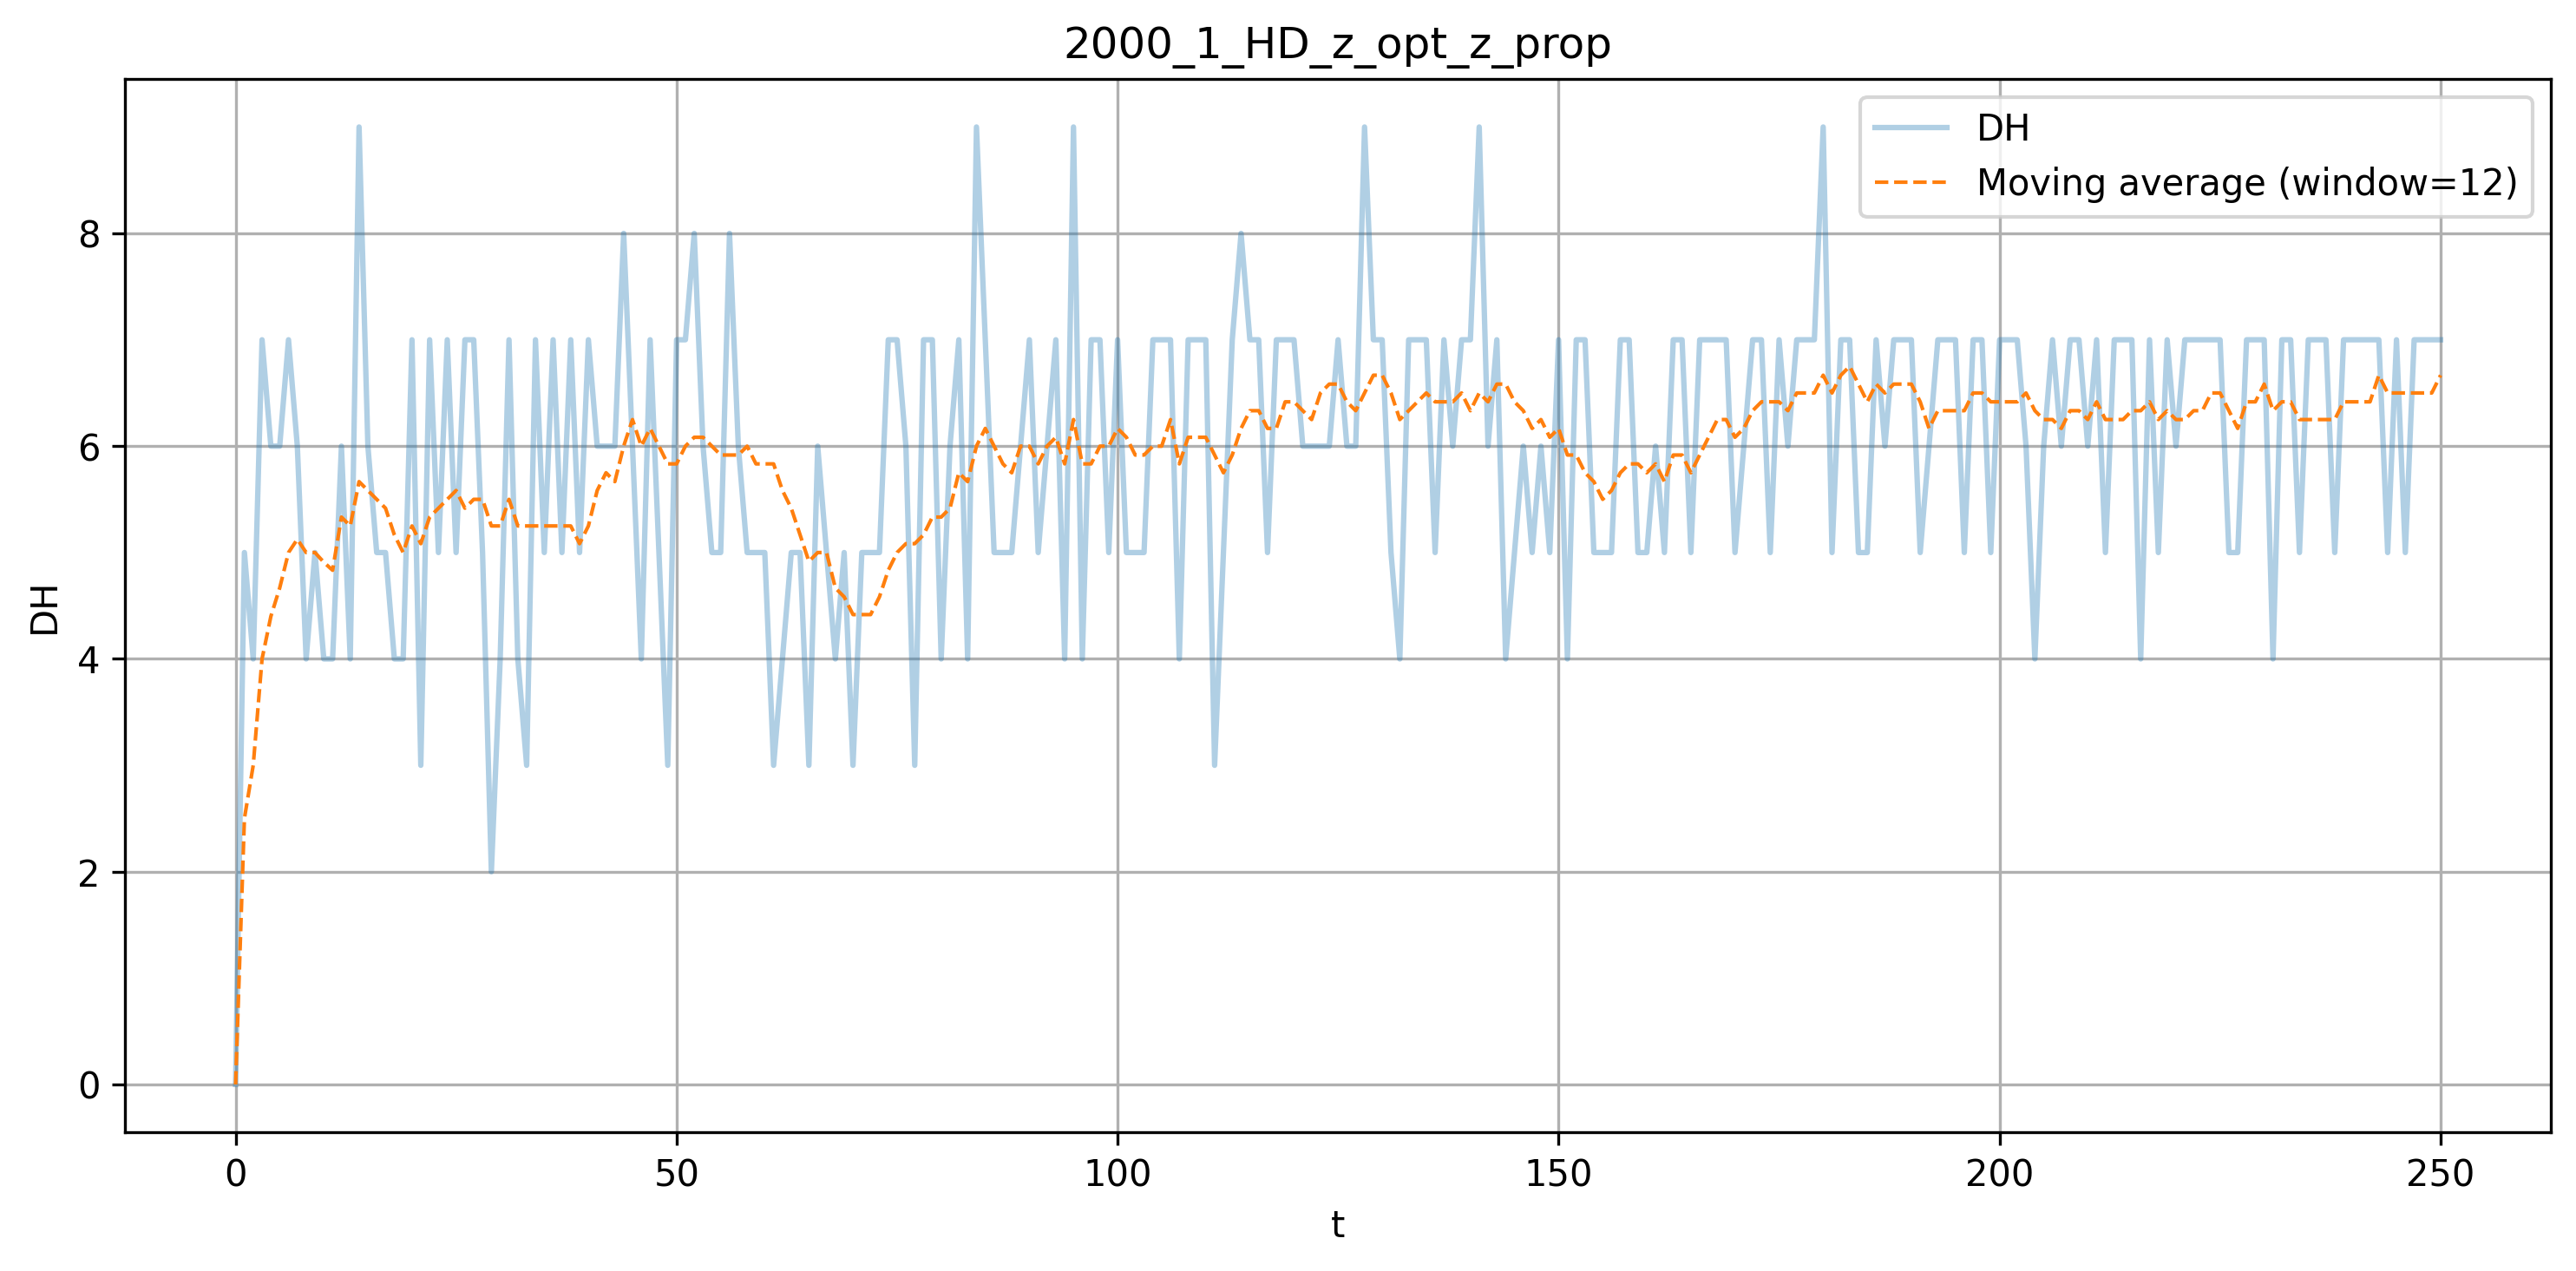
\includegraphics[width=\linewidth]{../Quantum-Annealing-for-solving-QUBO-Problems/test/Diagnostica_QALS/2/ksp_1/lambda_div_3/2000_1_HD_z_opt_z_prop.png}
    \caption{\(d_H(z_{opt}, z_t)\) con \(\lambda_2\)}
    \label{fig:hd-zopt-zprop-lambda2}
\end{subfigure}

\vspace{0.35cm}

\begin{subfigure}{0.495\textwidth}
    \centering
    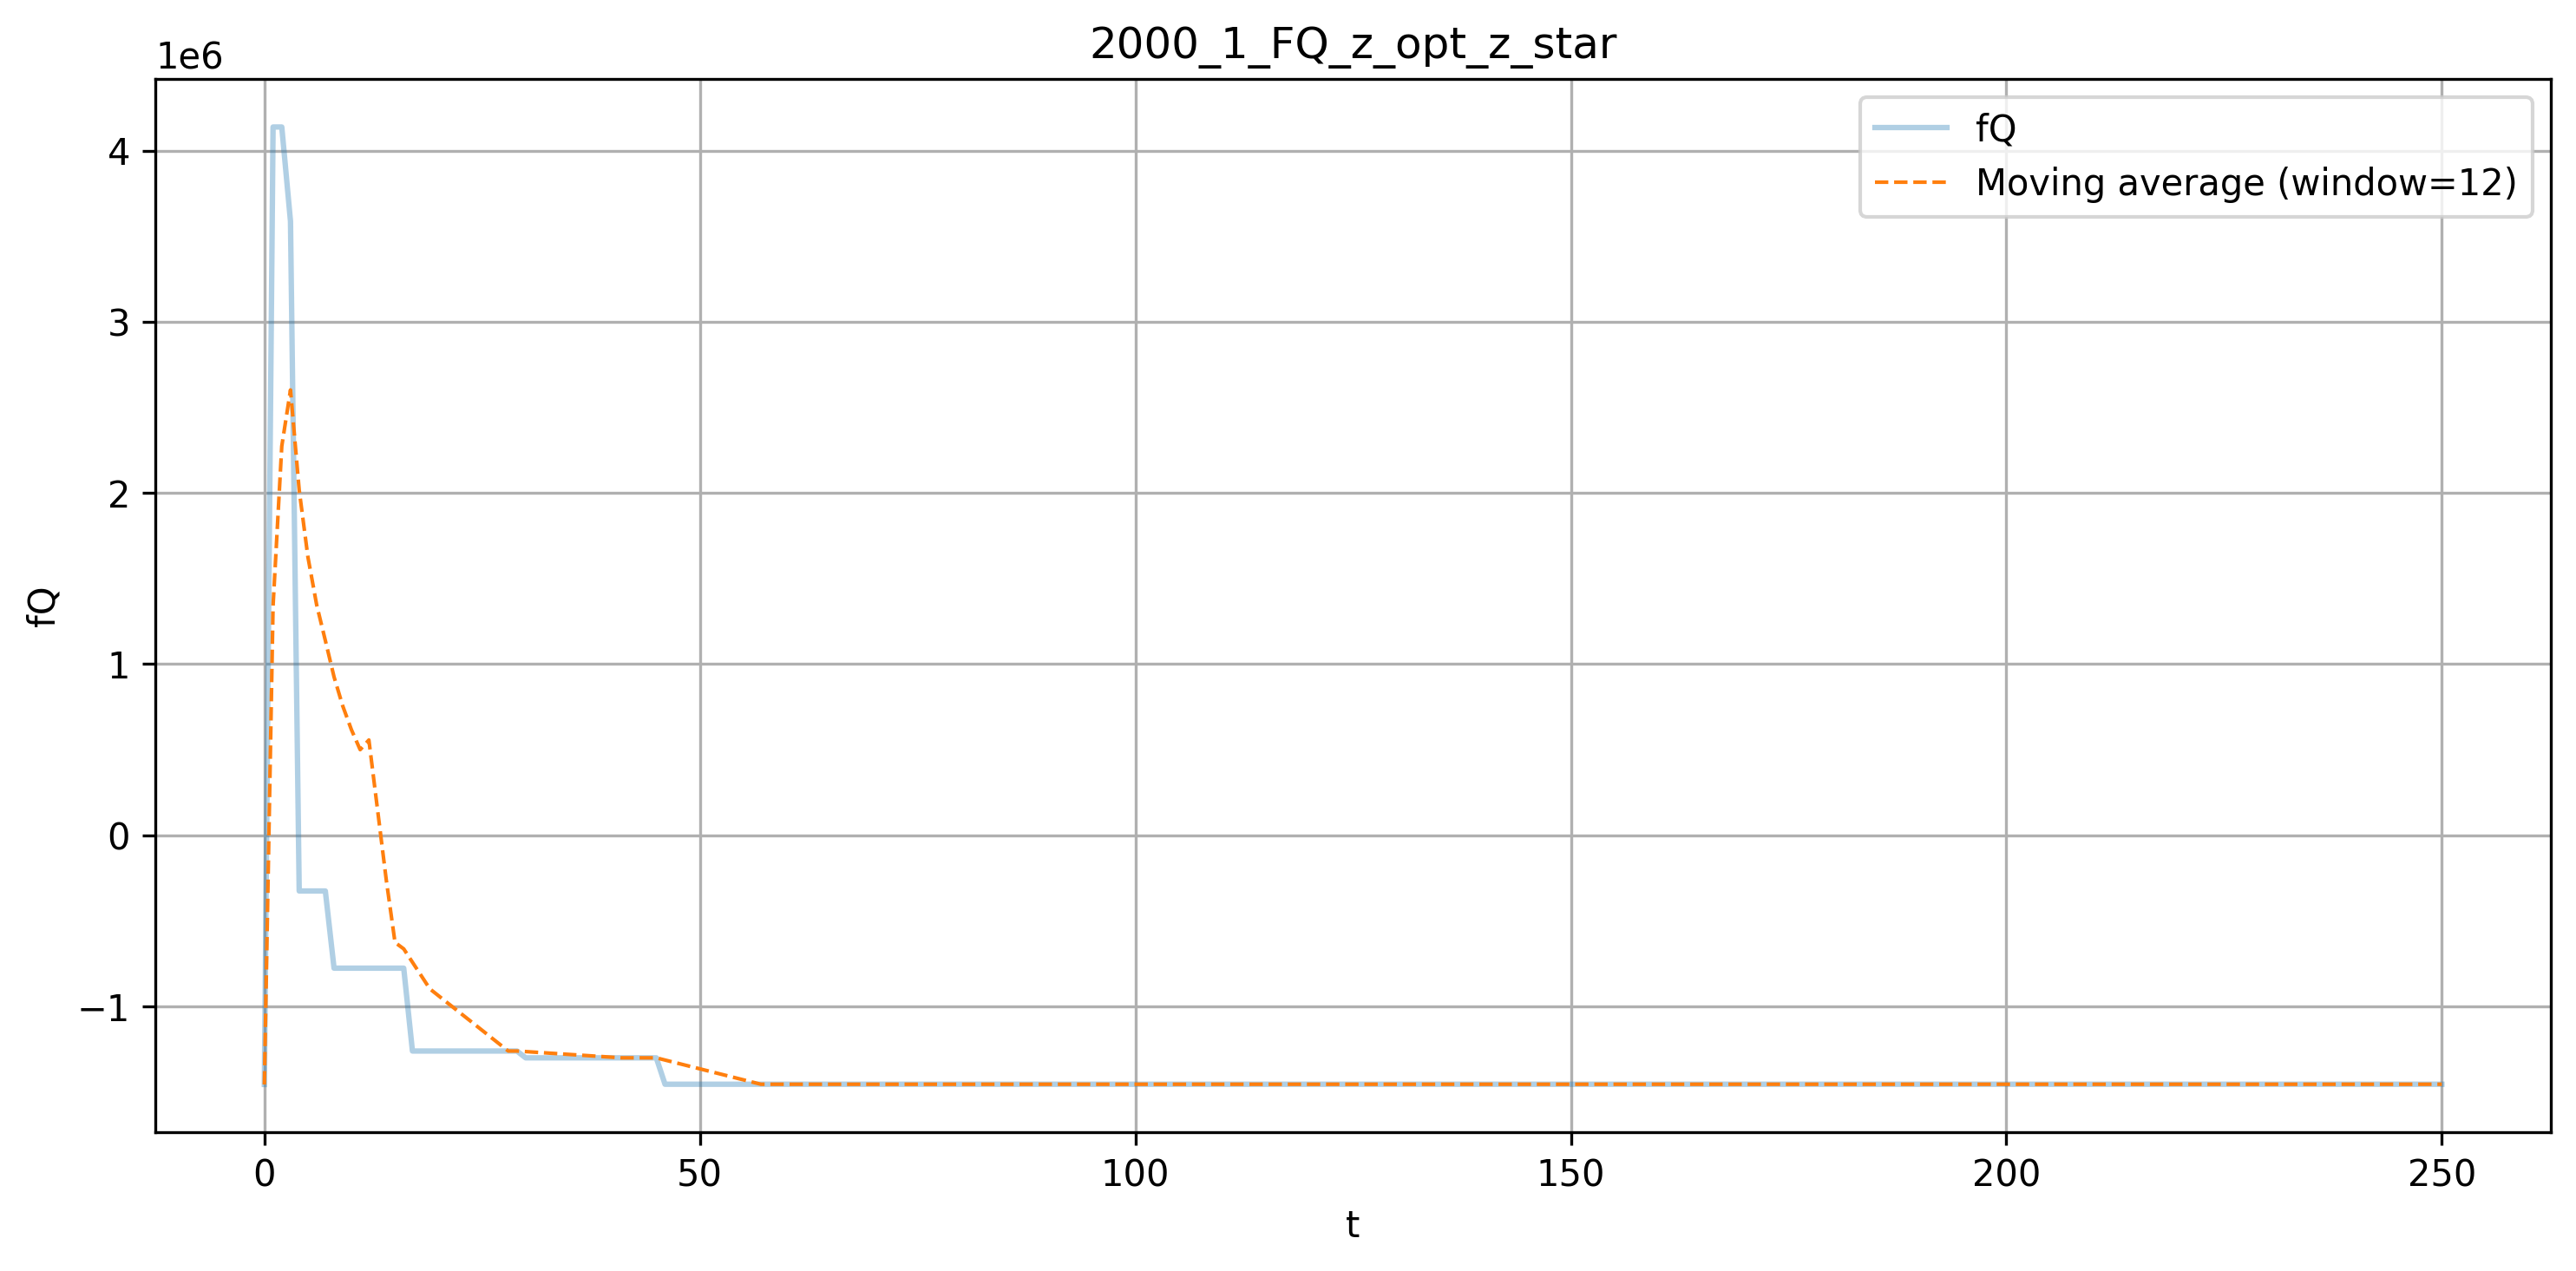
\includegraphics[width=\linewidth]{../Quantum-Annealing-for-solving-QUBO-Problems/test/Diagnostica_QALS/2/ksp_1/lambda_div_3/2000_1_FQ_z_opt_z_star.png}
    \caption{\(f_Q(z_\star)\) con \(\lambda_2\)}
    \label{fig:fQ-zstar-lambda2}
\end{subfigure}
\hfill
\begin{subfigure}{0.495\textwidth}
    \centering
    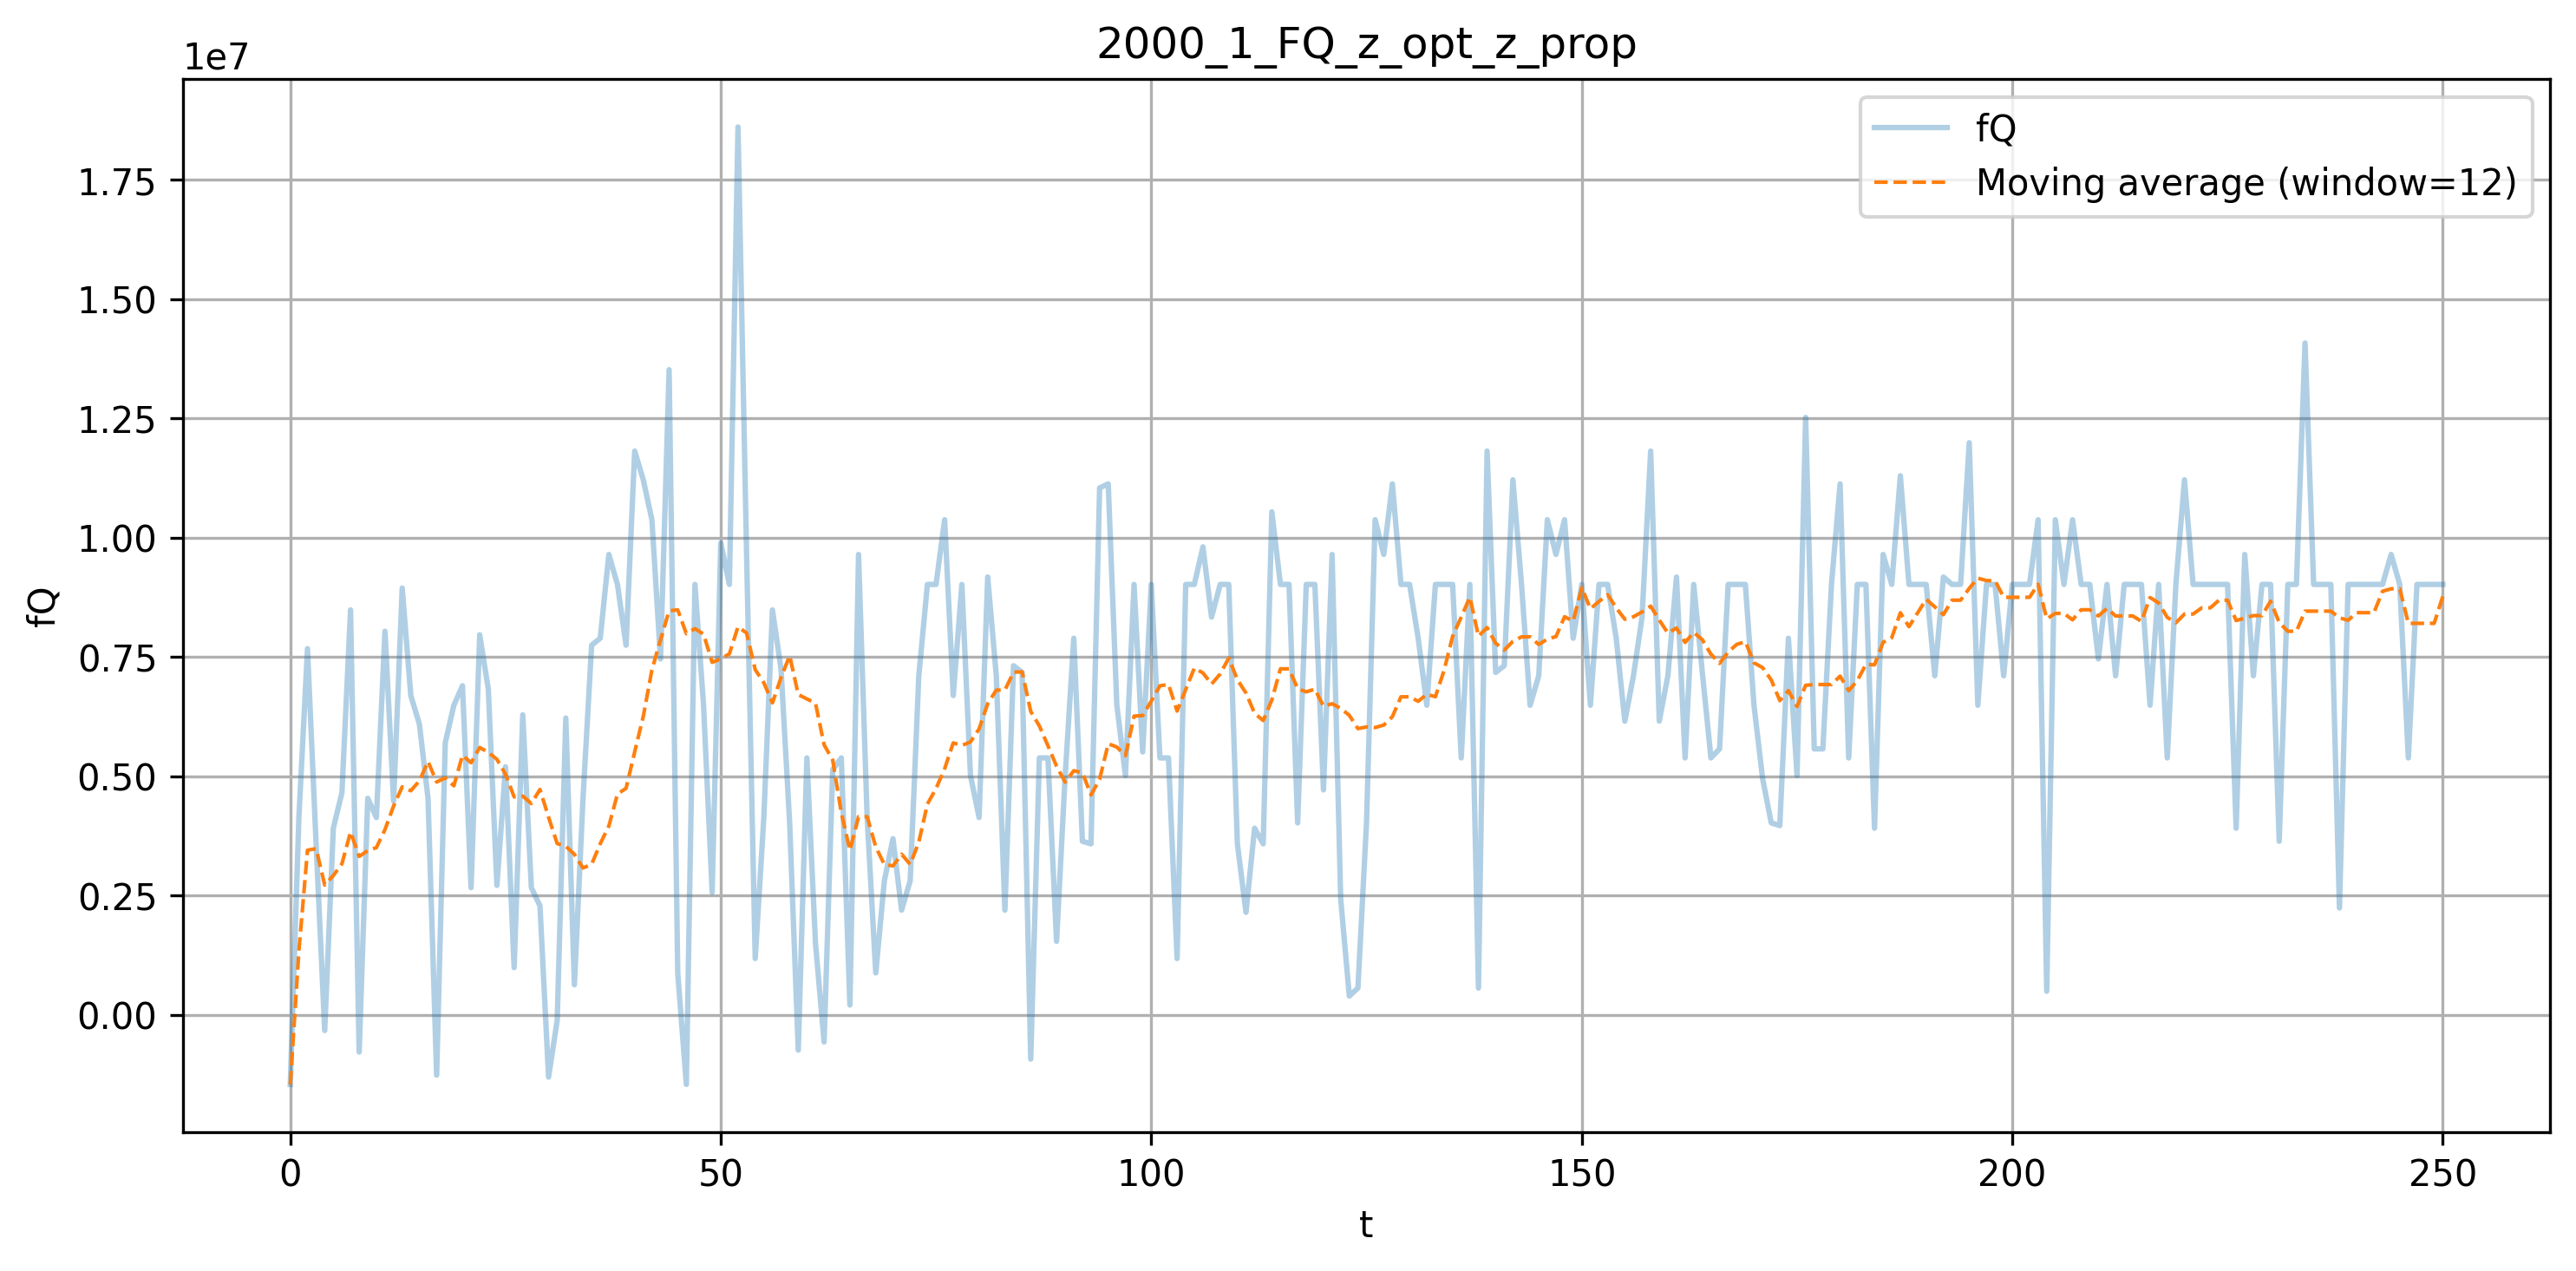
\includegraphics[width=\linewidth]{../Quantum-Annealing-for-solving-QUBO-Problems/test/Diagnostica_QALS/2/ksp_1/lambda_div_3/2000_1_FQ_z_opt_z_prop.png}
    \caption{\(f_Q(z_t)\) con \(\lambda_2\)}
    \label{fig:fQ-zt-lambda2}
\end{subfigure}
\label{fig:confronto-hamming-ksp12}
\end{figure}

\begin{figure}[H]
\centering
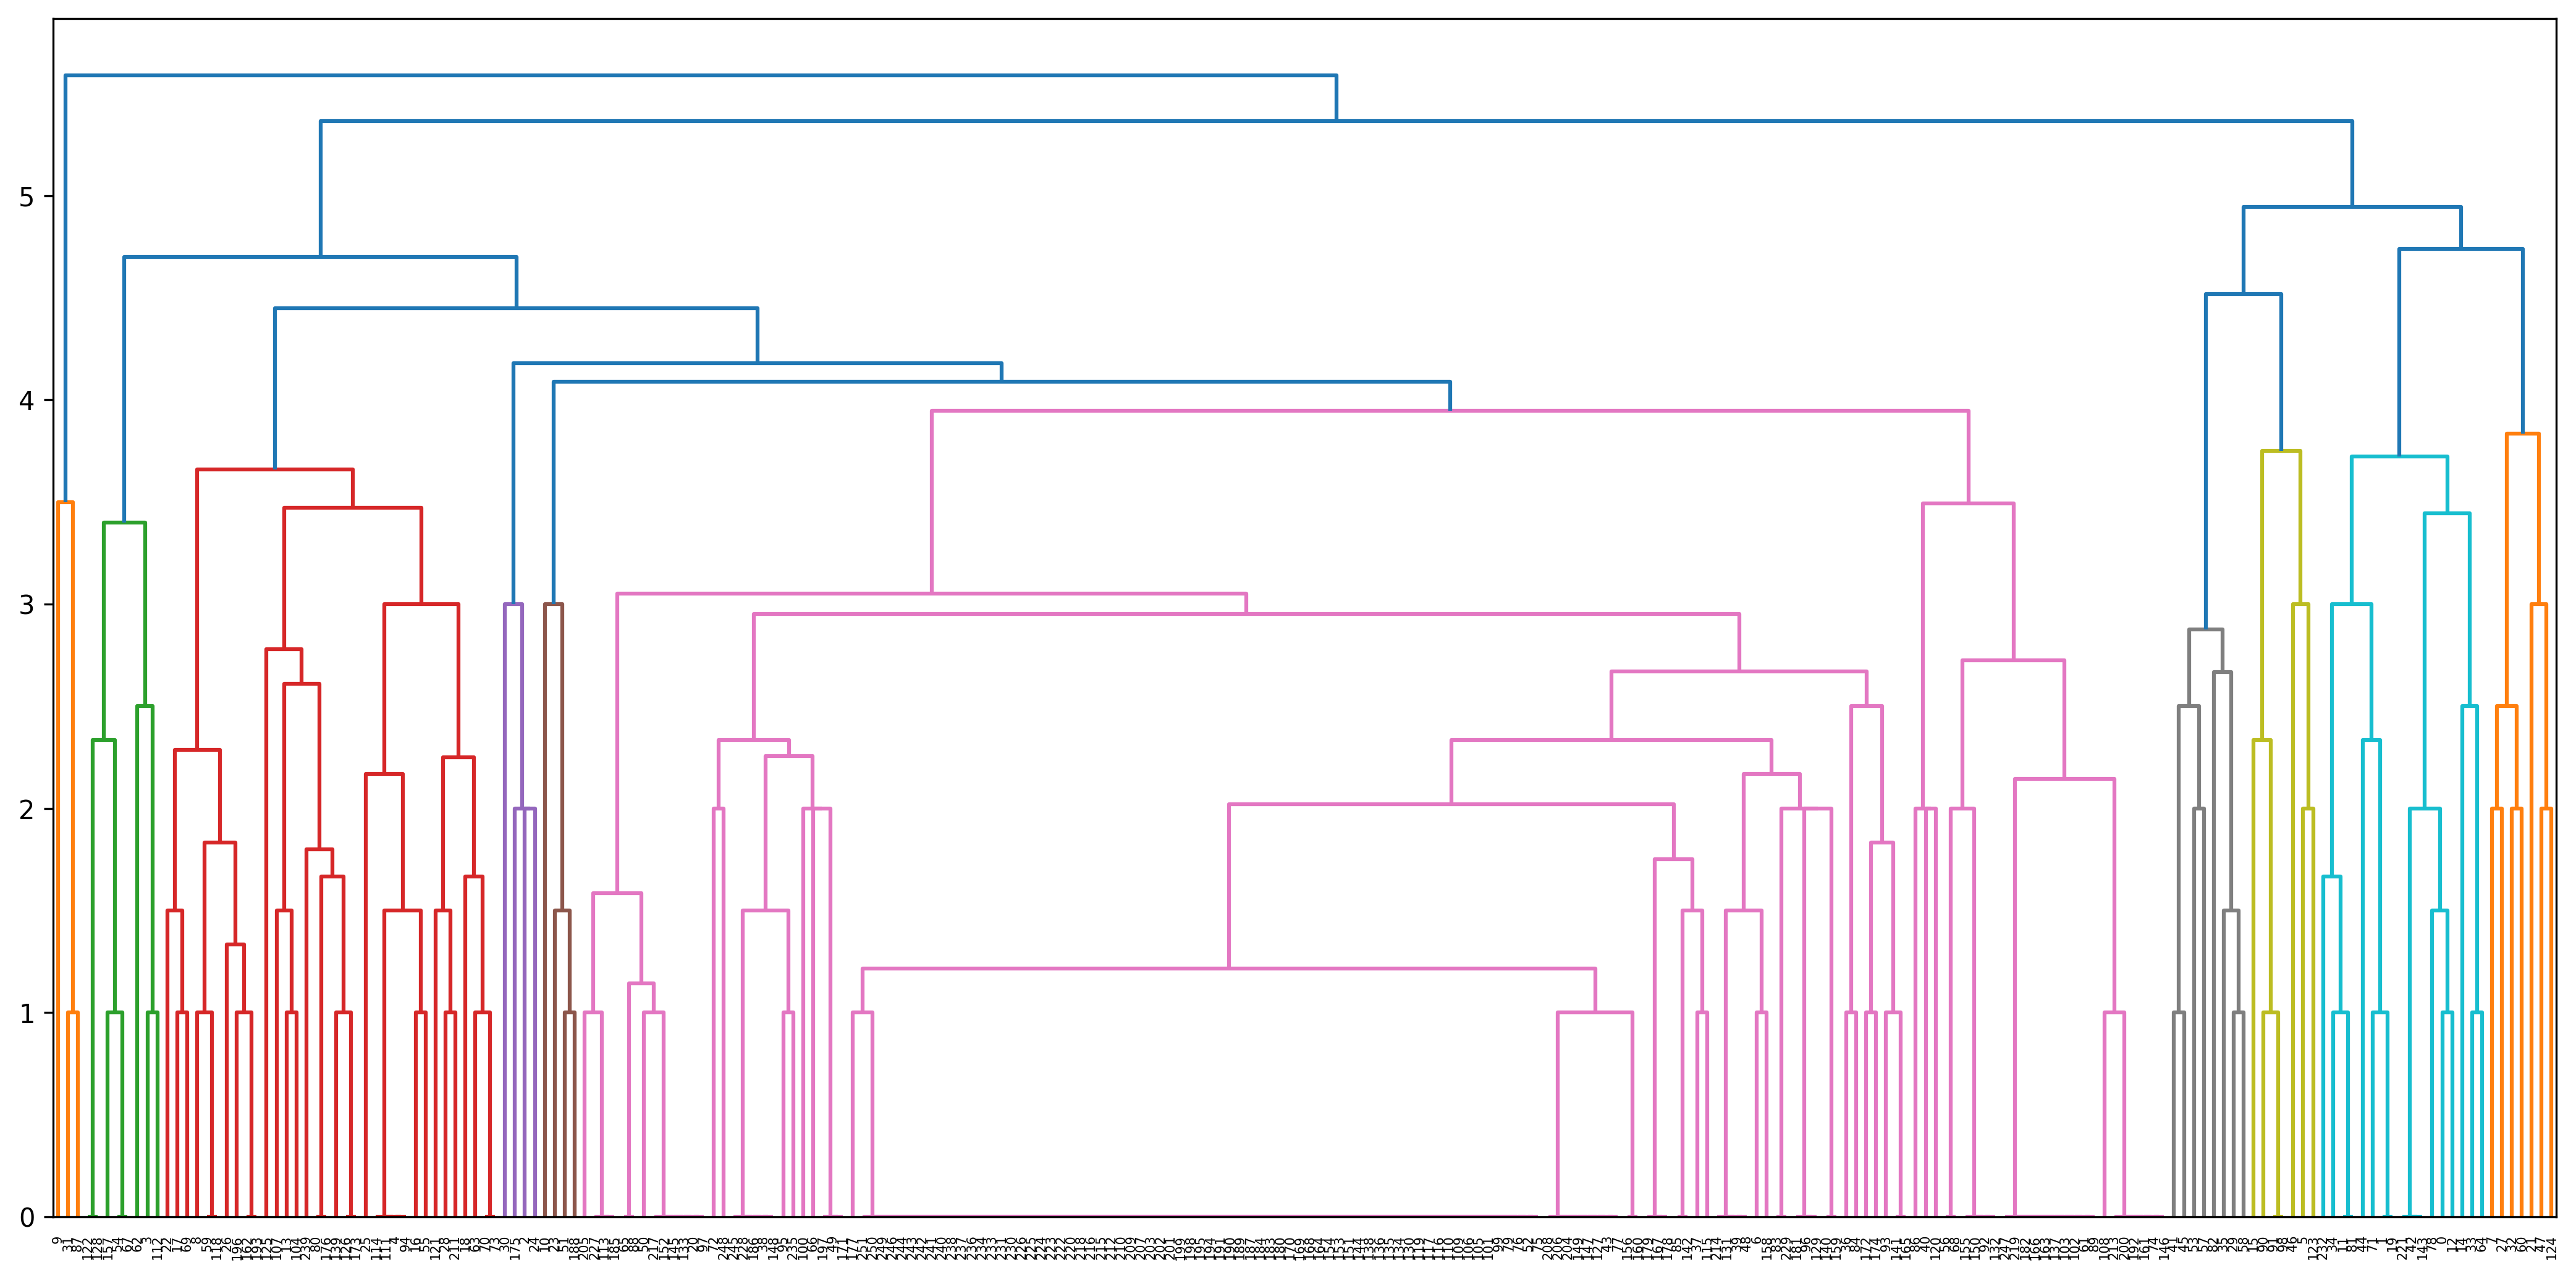
\includegraphics[width=\linewidth]{../Quantum-Annealing-for-solving-QUBO-Problems/test/Diagnostica_QALS/2/ksp_1/lambda_div_3/dendrogram_2000_1.png}
\caption{Agglomerative Clustering Dendogram}
\label{fig:AgglomerativeClustering-ksp1}
\end{figure}

\clearpage
\subsection{ksp\_3}

\begin{table}[h]
\centering
\begin{tabular}{lcc}
\hline
\textbf{Metrica} & \(\lambda_1\) & \(\lambda_2\) \\
\hline
Numero cluster & 29 & 30 \\
Dimensione cluster massimo & 73 & 110 \\
Cluster z best & 15 & 17 \\
Single clusters & 1 & 0 \\
\(f_Q\) medoid & 396906.49 & 50443988075.67 \\
Profit medoid & 5330 & 4928 \\
Weight medoid & 4450 & 2830 \\
\hline
\(f_Q\) Min Found QALS & 89157.79 & 4487337042.67 \\
Profit Found QALS & 2621 & 3261 \\
Weight Found QALS & 2438 & 1853 \\
\hline
\(f_Q\) Min Found NO QALS & -9424.80 & -714267662.00 \\
Profit Found NO QALS & 2936 & 2483 \\
Weight Found NO QALS & 560 & 501 \\
\hline
\end{tabular}
\caption{Confronto dei risultati ottenuti con QALS e senza QALS.}
\label{tab:confronto-qals-noqals-ksp}
\end{table}

\begin{figure}[H]
\centering
\begin{subfigure}{0.495\textwidth}
    \centering
    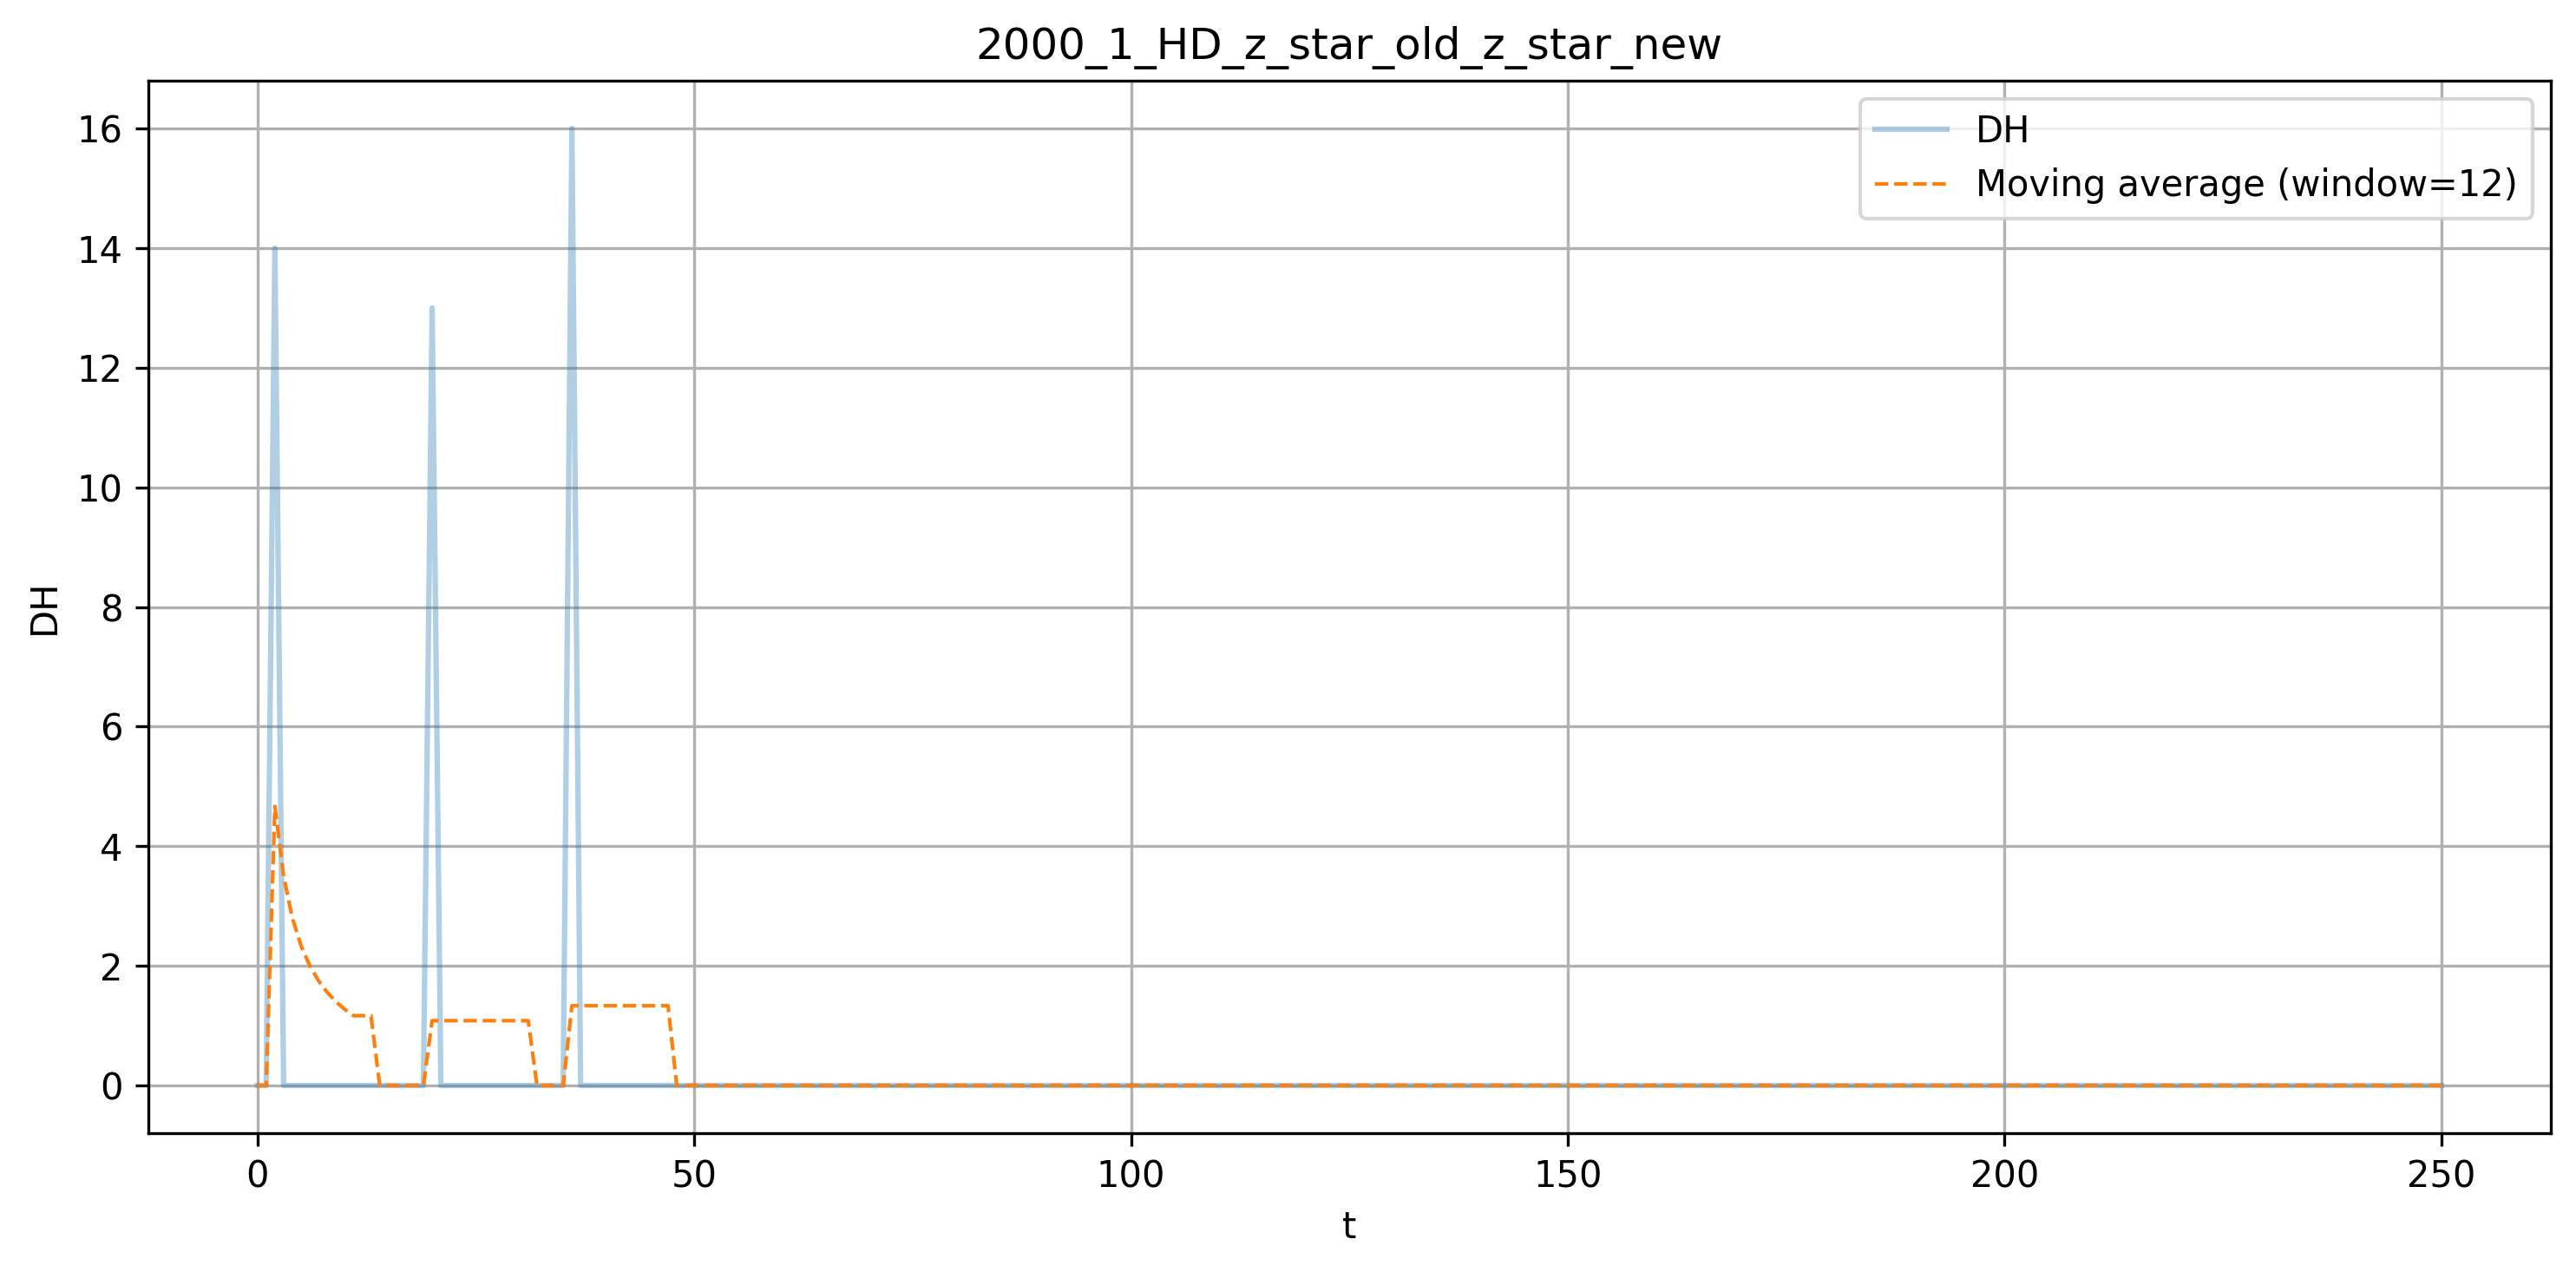
\includegraphics[width=\linewidth]{../Quantum-Annealing-for-solving-QUBO-Problems/test/Diagnostica_QALS/2/ksp_3/lambda_650_dot_C/2000_1_HD_z_star_old_z_star_new.png}
    \caption{\(d_H(z_\star^{old}, z_\star^{new})\) con \(\lambda_1\)}
    \label{fig:hd-zstarold-zstarnew-lambda1}
\end{subfigure}
\hfill
\begin{subfigure}{0.495\textwidth}
    \centering
    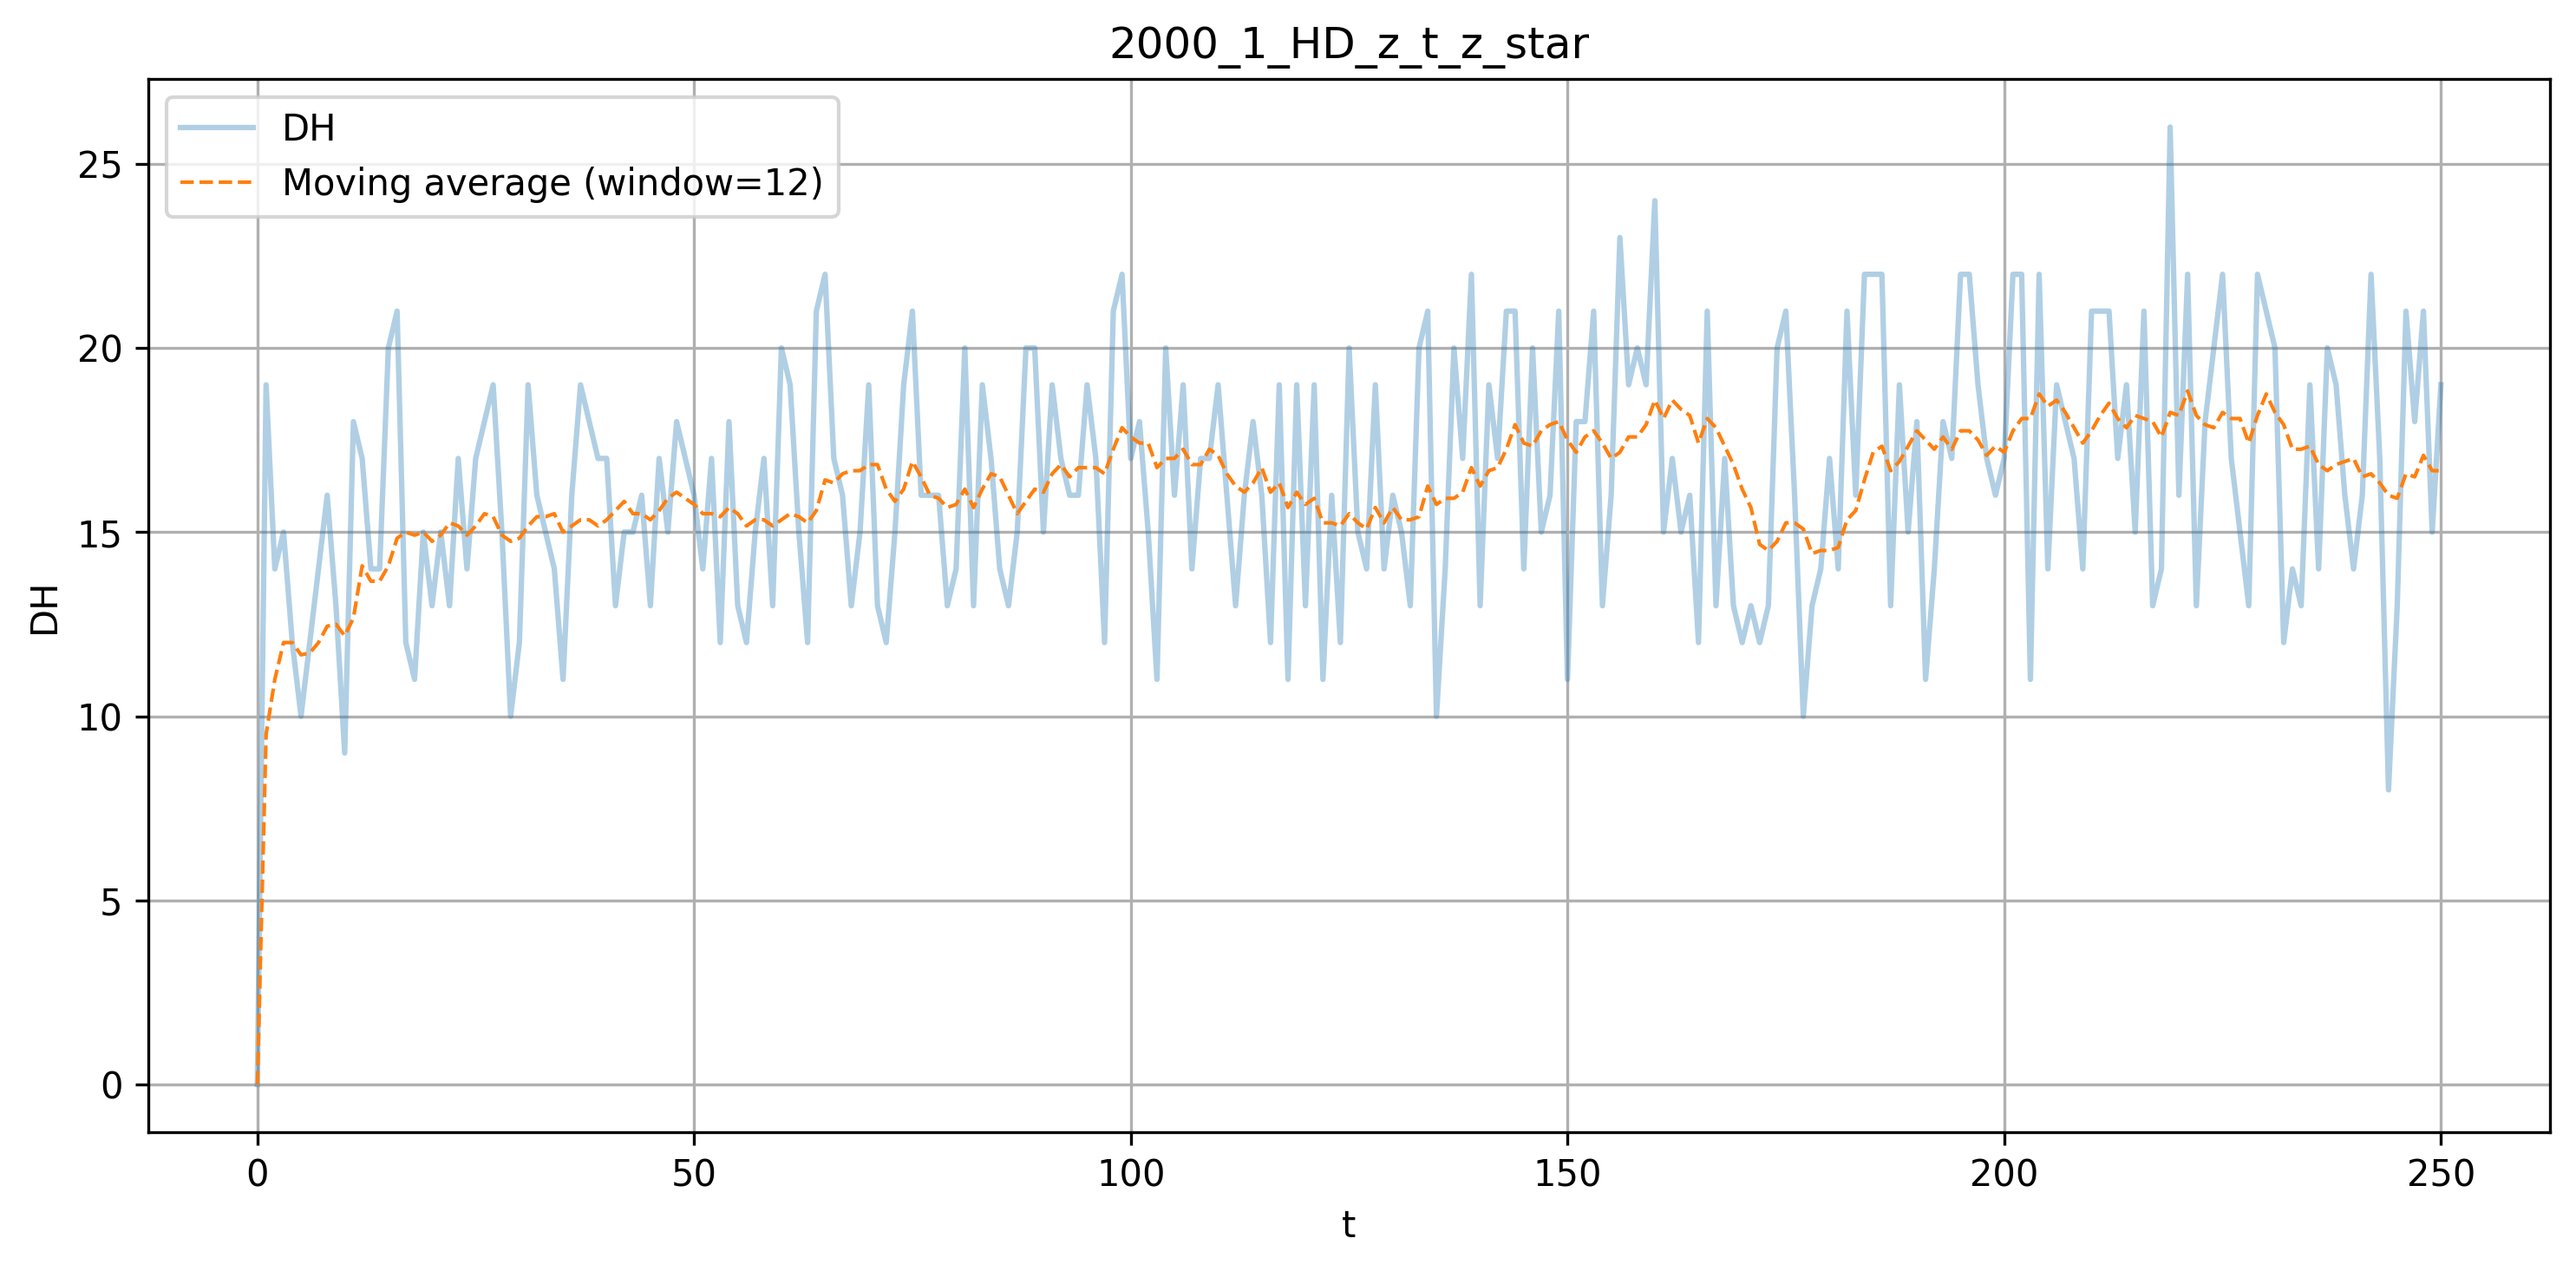
\includegraphics[width=\linewidth]{../Quantum-Annealing-for-solving-QUBO-Problems/test/Diagnostica_QALS/2/ksp_3/lambda_650_dot_C/2000_1_HD_z_t_z_star.png}
    \caption{\(d_H(z_t, z_\star)\) con \(\lambda_1\)}
    \label{fig:hd-zt-zstar-lambda1}
\end{subfigure}

\vspace{0.35cm}

\begin{subfigure}{0.495\textwidth}
    \centering
    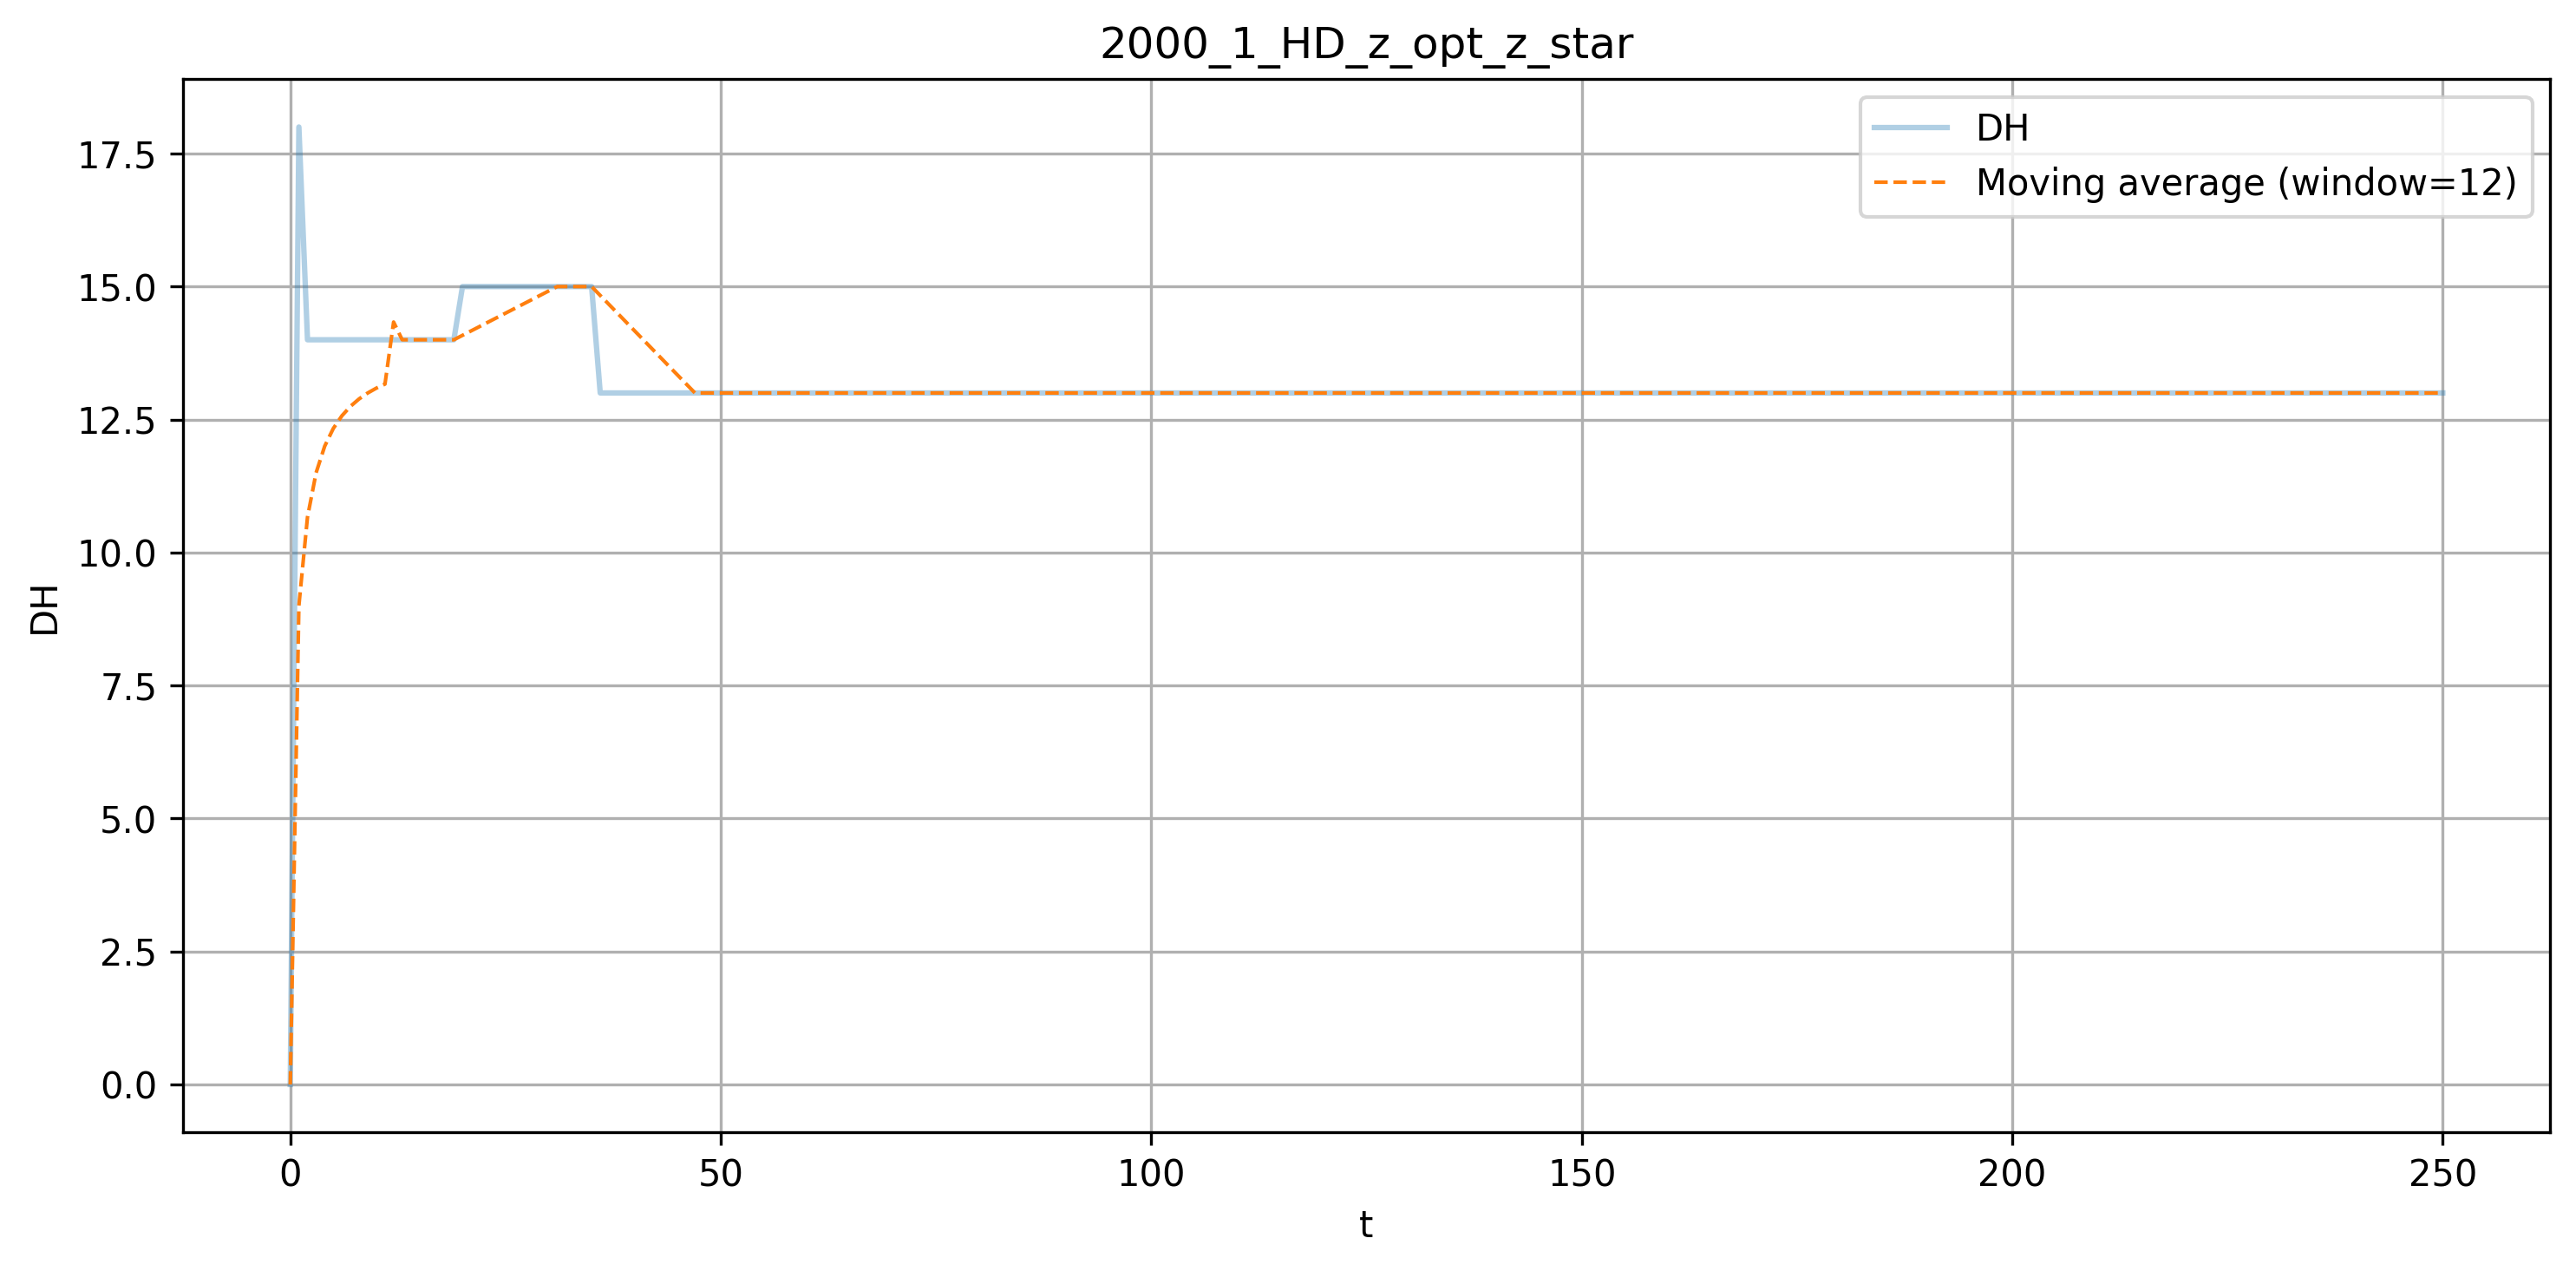
\includegraphics[width=\linewidth]{../Quantum-Annealing-for-solving-QUBO-Problems/test/Diagnostica_QALS/2/ksp_3/lambda_650_dot_C/2000_1_HD_z_opt_z_star.png}
    \caption{\(d_H(z_{opt}, z_\star)\) con \(\lambda_1\)}
    \label{fig:hd-zopt-zstar-lambda1}
\end{subfigure}
\hfill
\begin{subfigure}{0.495\textwidth}
    \centering
    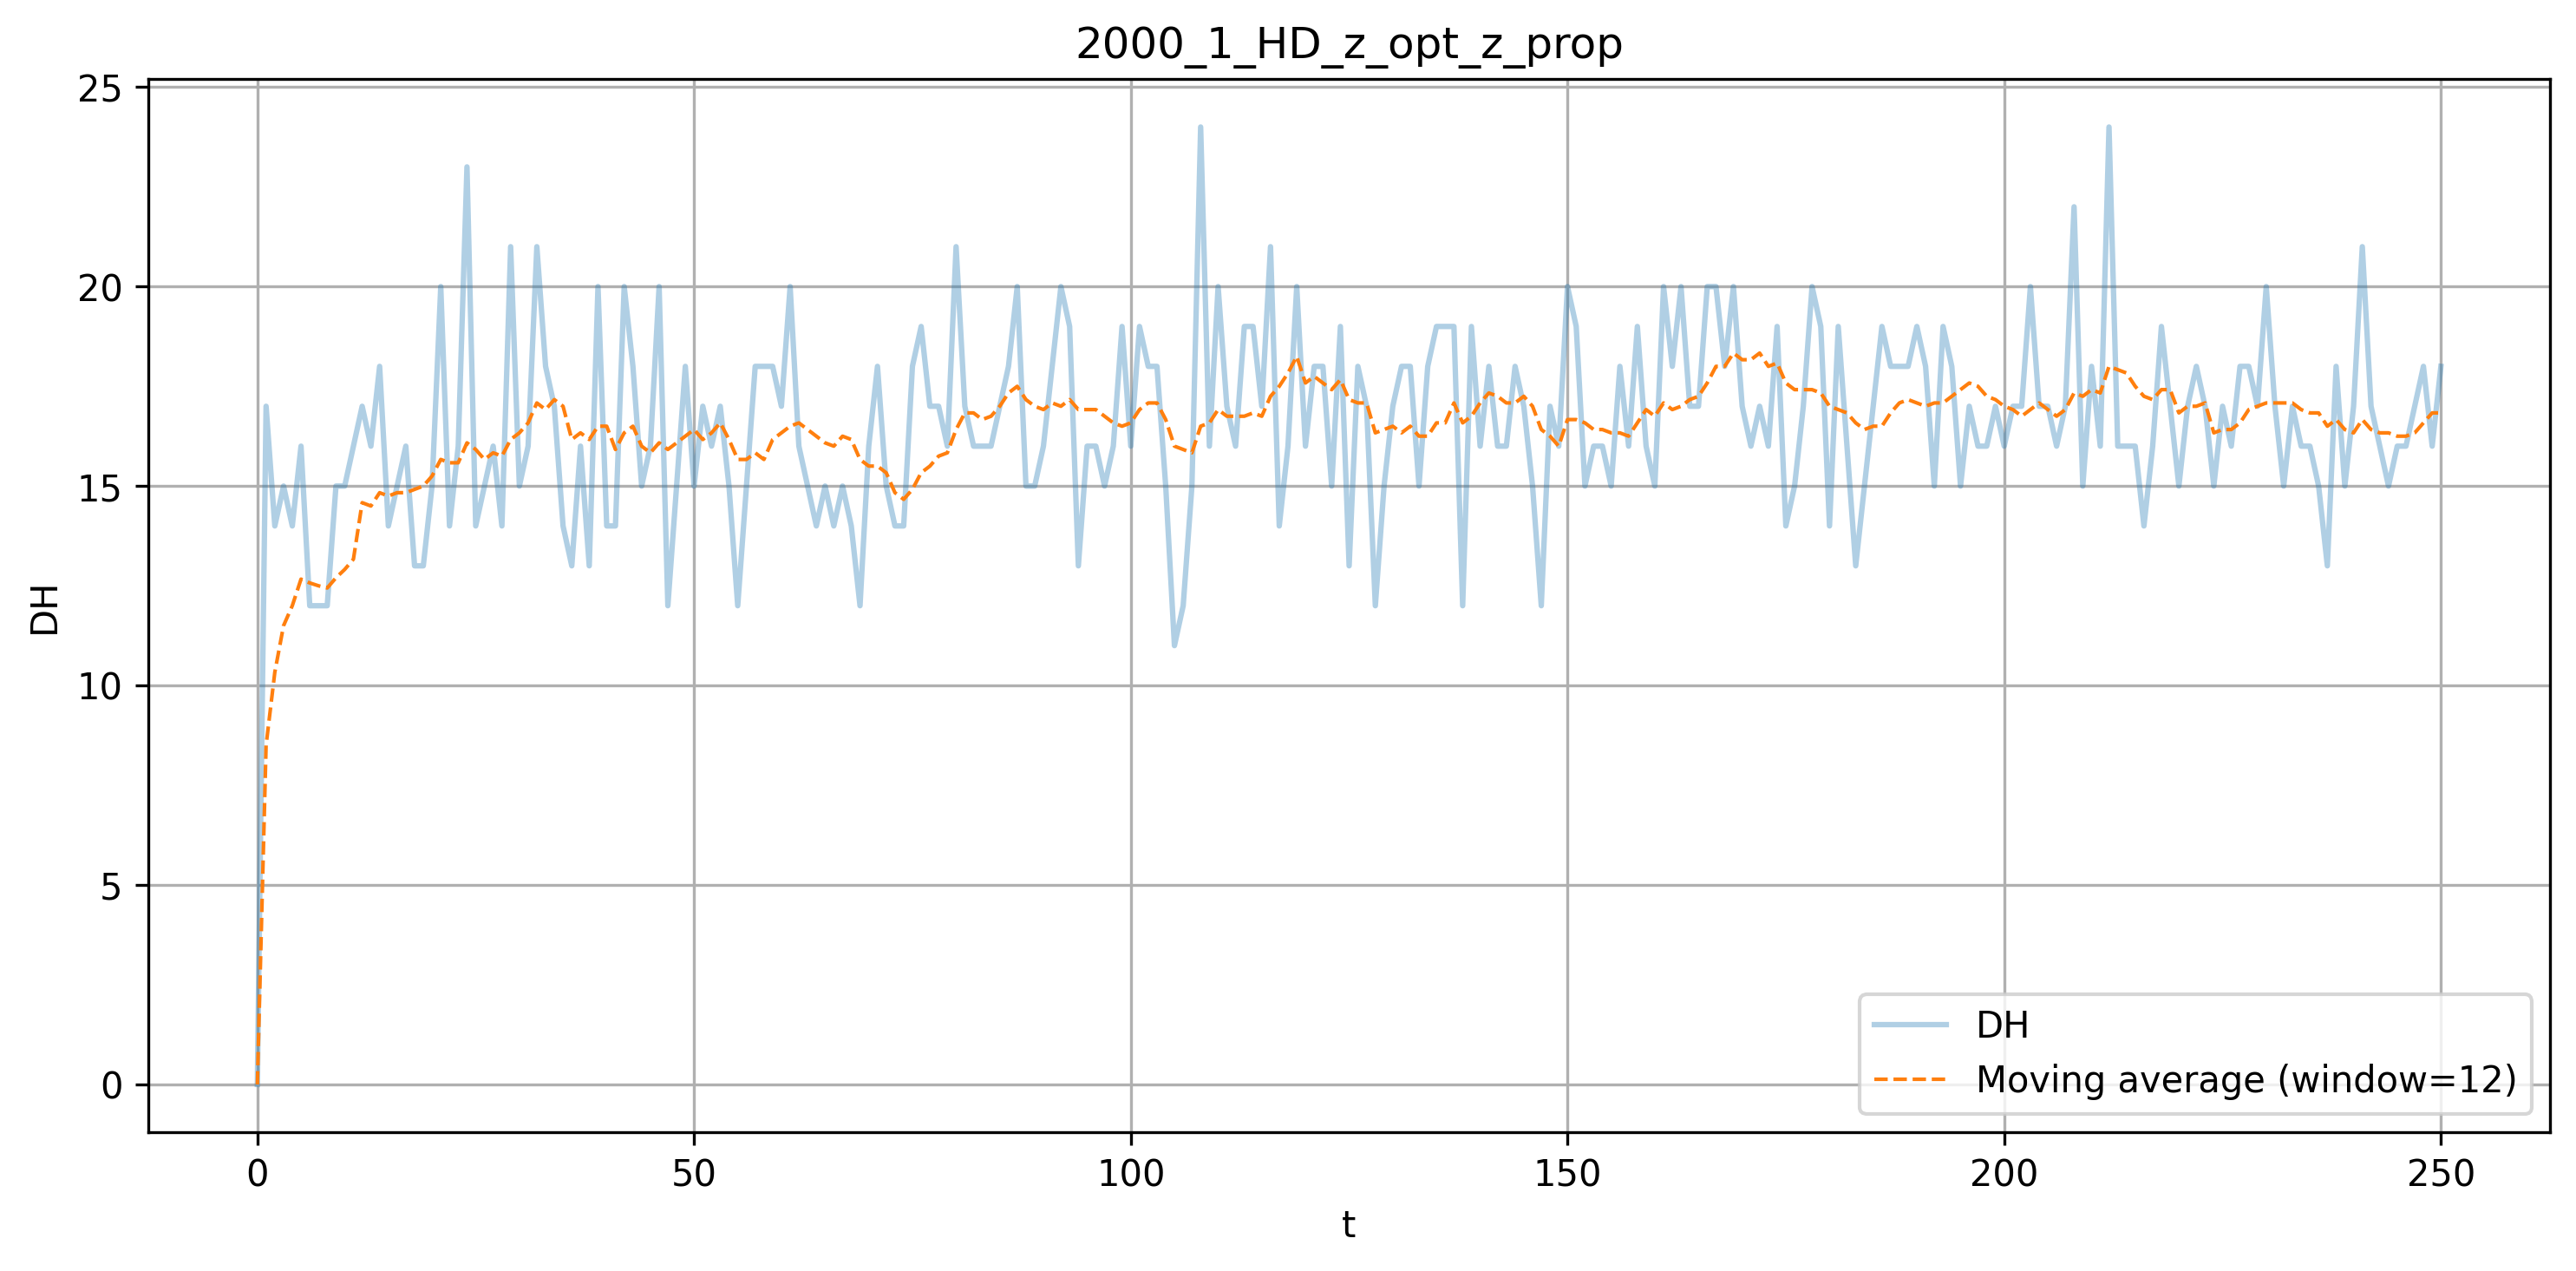
\includegraphics[width=\linewidth]{../Quantum-Annealing-for-solving-QUBO-Problems/test/Diagnostica_QALS/2/ksp_3/lambda_650_dot_C/2000_1_HD_z_opt_z_prop.png}
    \caption{\(d_H(z_{opt}, z_t)\) con \(\lambda_1\)}
    \label{fig:hd-zopt-zt-lambda1}
\end{subfigure}

\vspace{0.35cm}

\begin{subfigure}{0.495\textwidth}
    \centering
    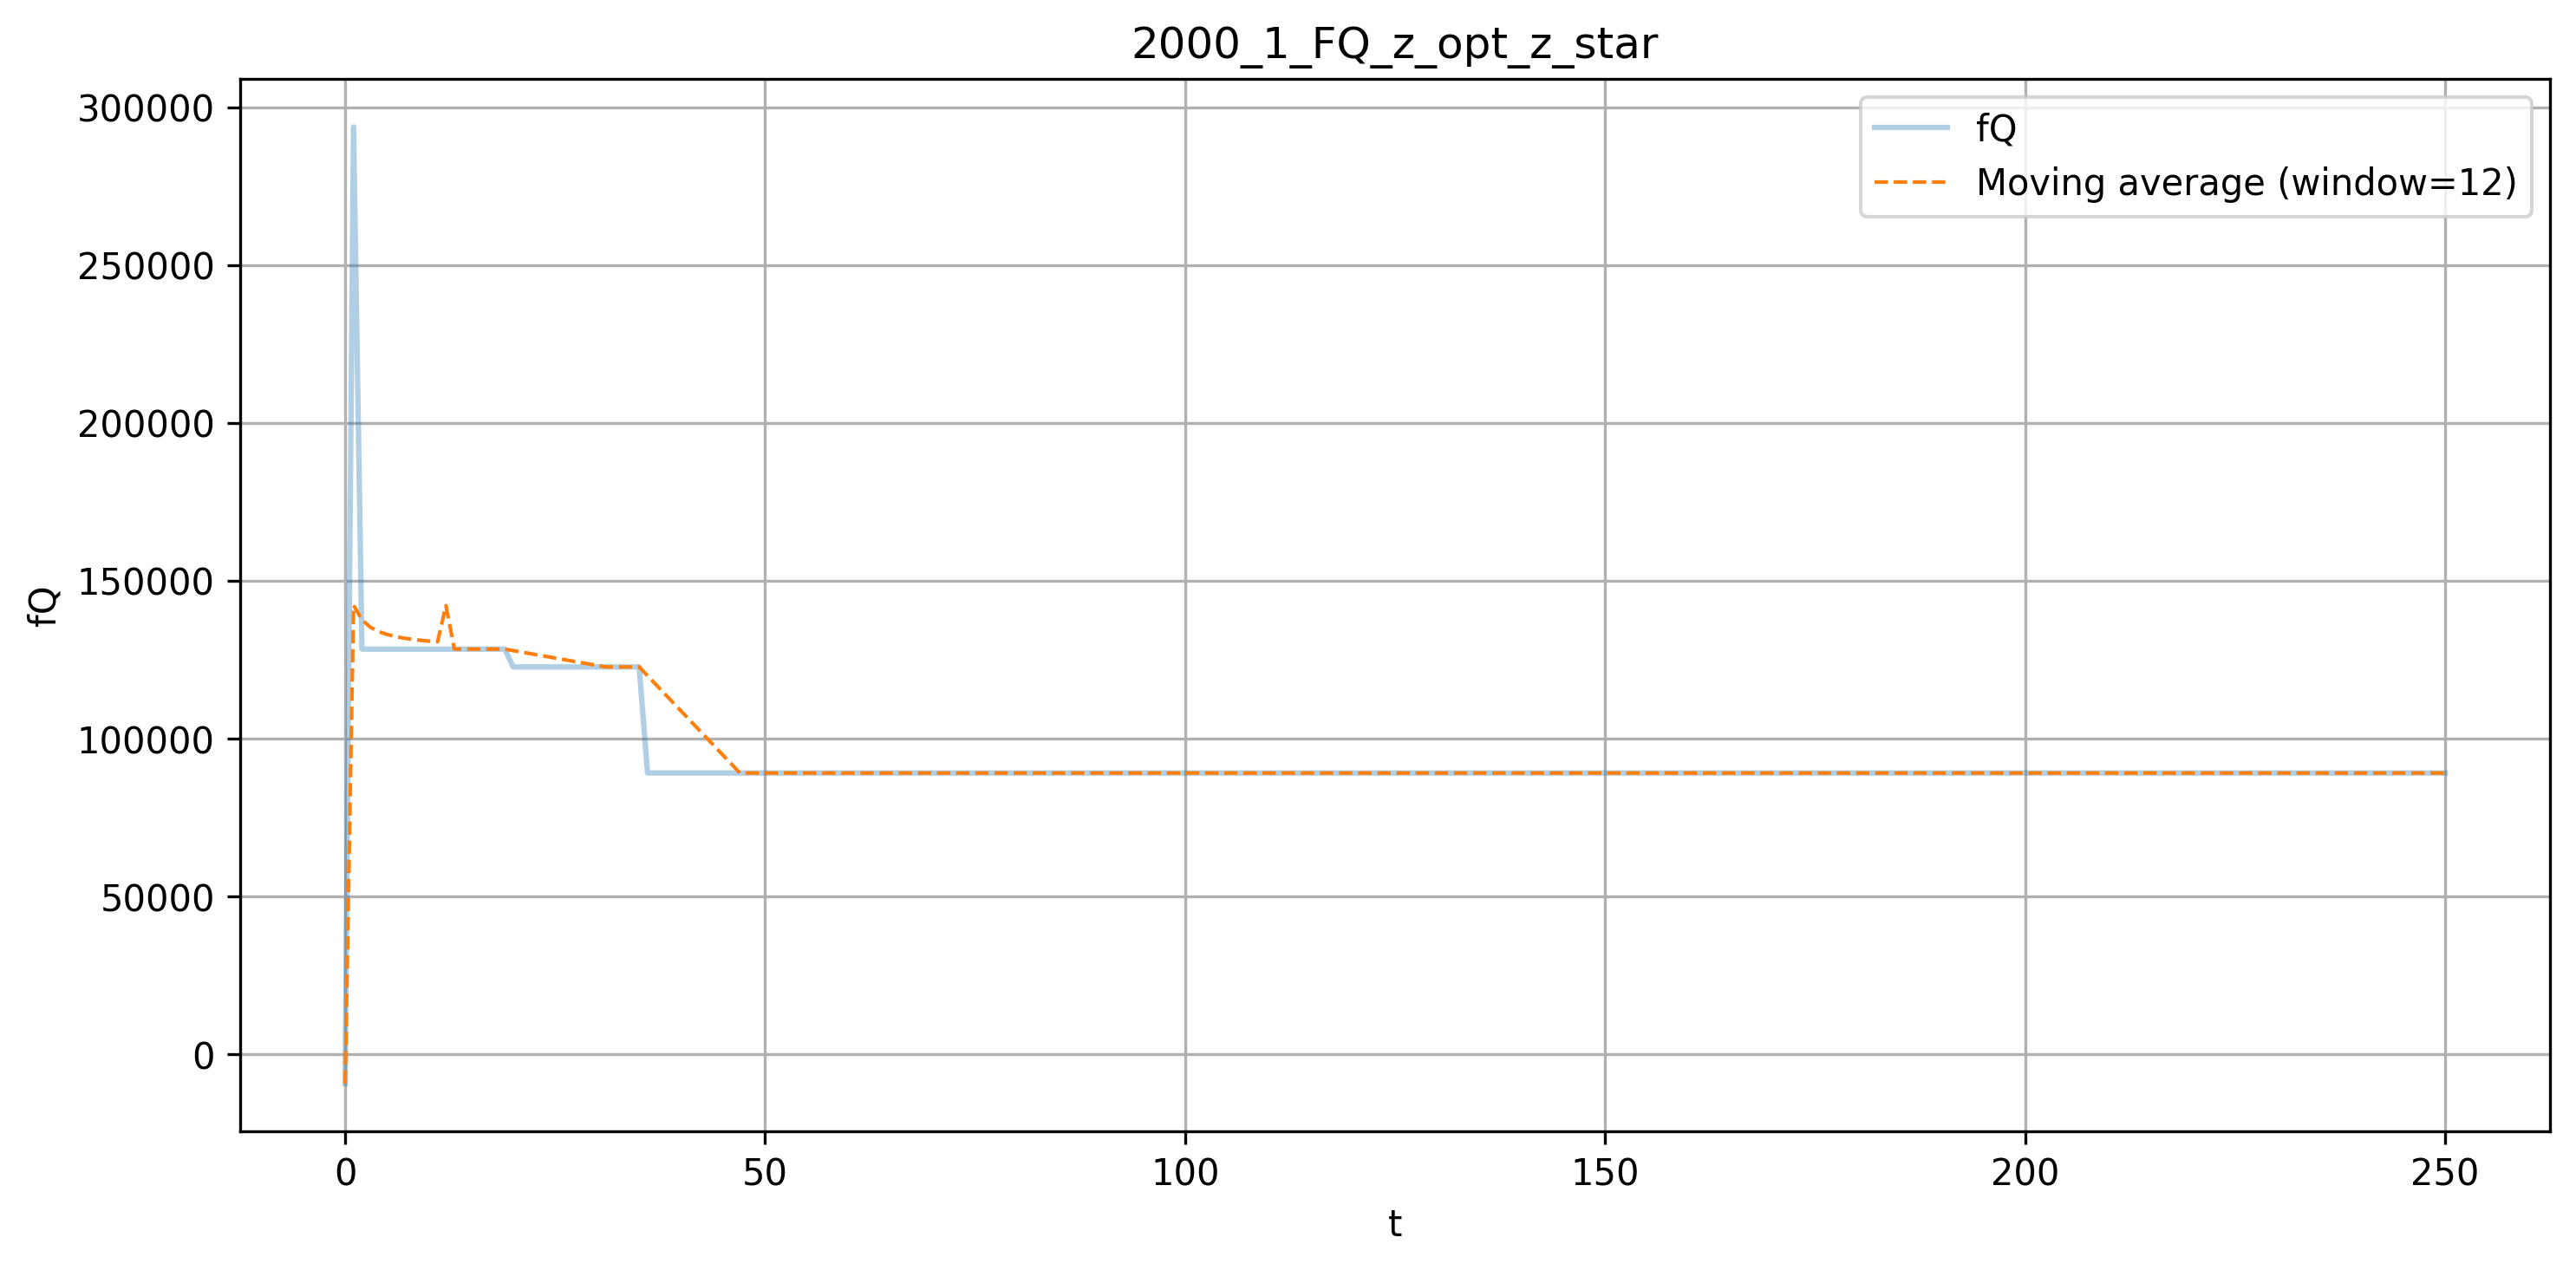
\includegraphics[width=\linewidth]{../Quantum-Annealing-for-solving-QUBO-Problems/test/Diagnostica_QALS/2/ksp_3/lambda_650_dot_C/2000_1_FQ_z_opt_z_star.png}
    \caption{\(f_Q(z_\star)\) con \(\lambda_1\)}
    \label{fig:fQ-zstar-lambda1}
\end{subfigure}
\hfill
\begin{subfigure}{0.495\textwidth}
    \centering
    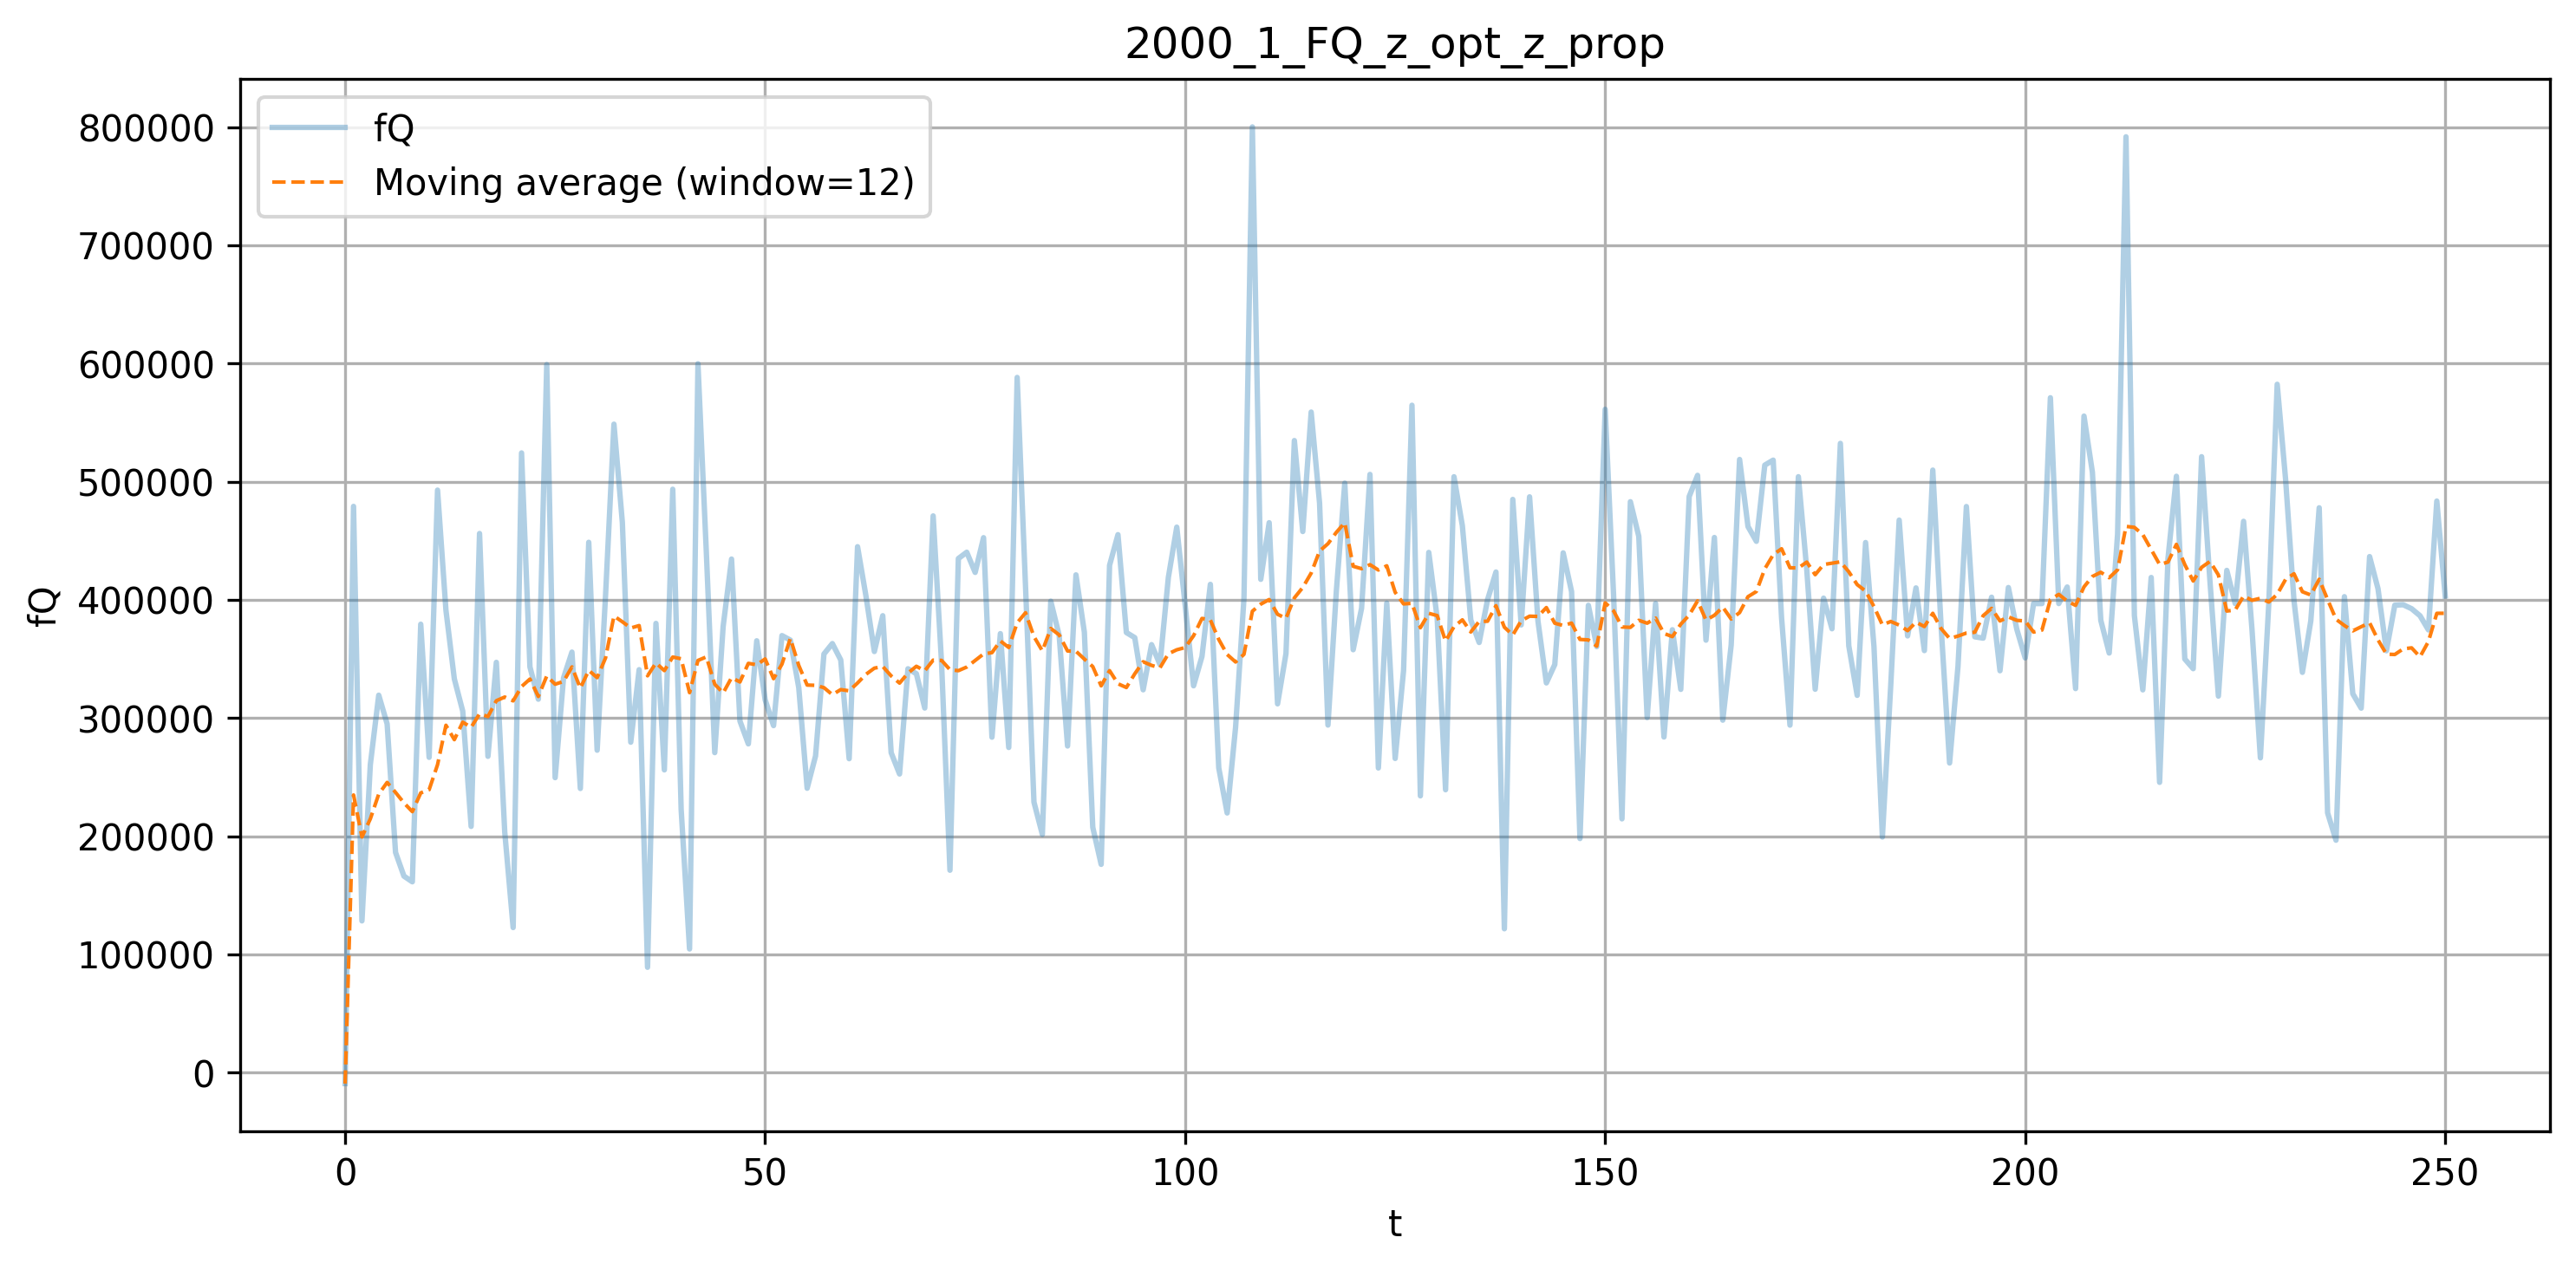
\includegraphics[width=\linewidth]{../Quantum-Annealing-for-solving-QUBO-Problems/test/Diagnostica_QALS/2/ksp_3/lambda_650_dot_C/2000_1_FQ_z_opt_z_prop.png}
    \caption{\(f_Q(z_t)\) con \(\lambda_1\)}
    \label{fig:fQ-zt-lambda1}
\end{subfigure}
\label{fig:confronto-hamming-ksp31}
\end{figure}

\begin{figure}[H]
\centering
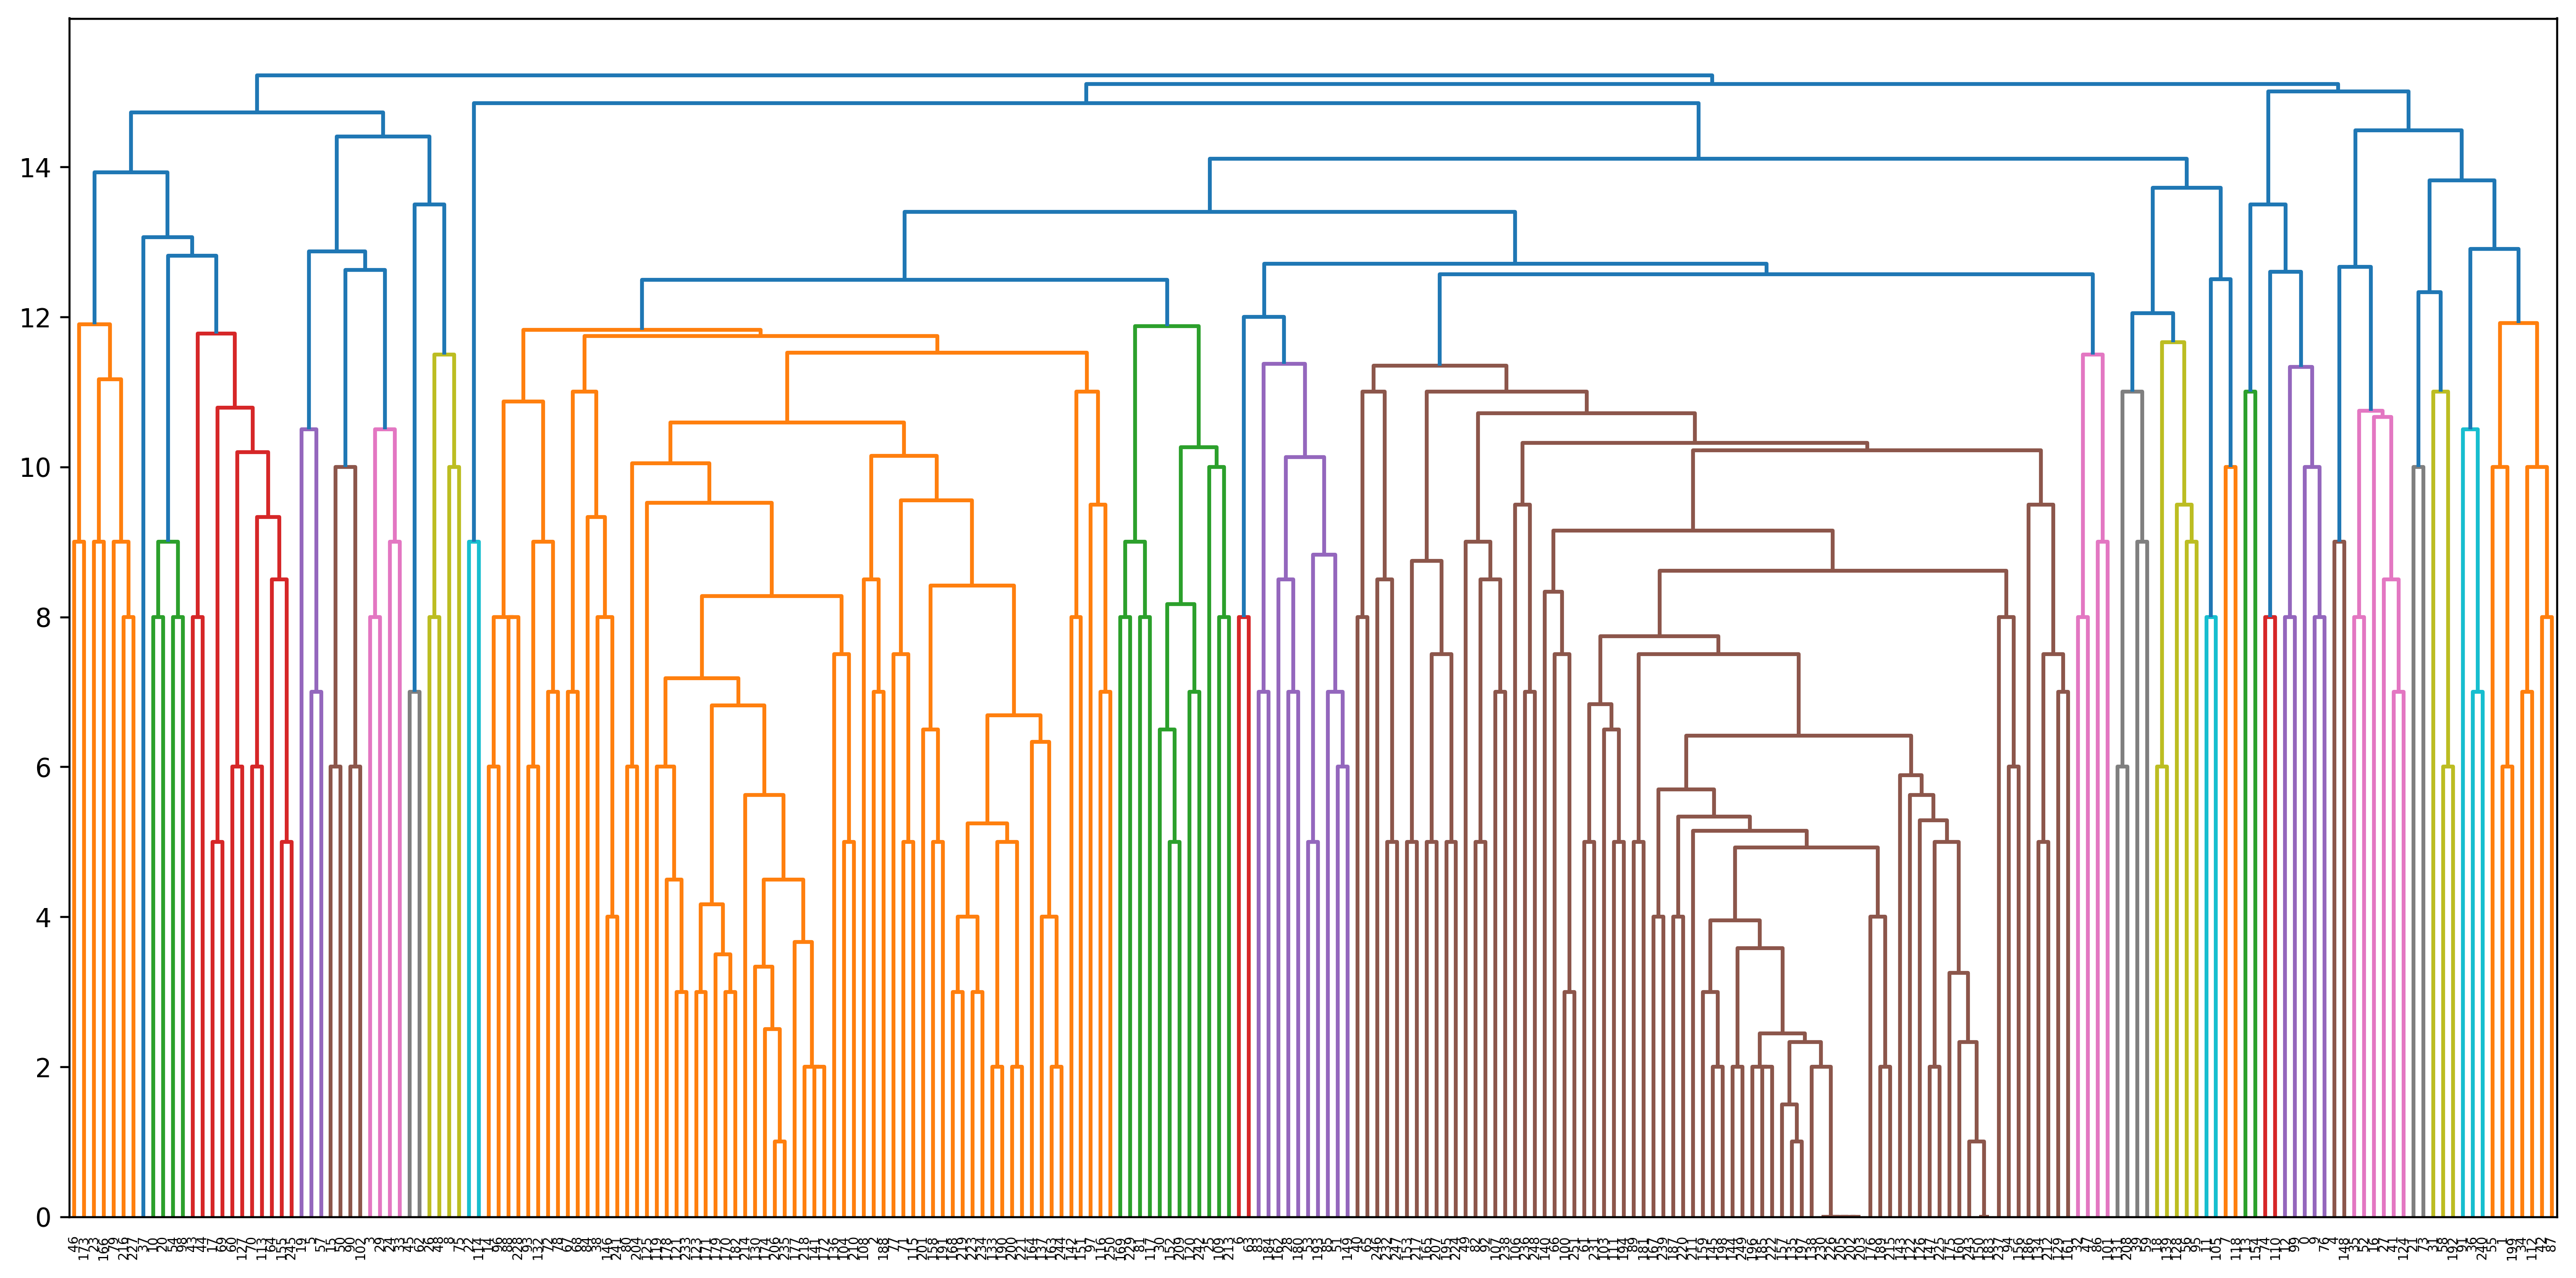
\includegraphics[width=\linewidth]{../Quantum-Annealing-for-solving-QUBO-Problems/test/Diagnostica_QALS/2/ksp_3/lambda_650_dot_C/dendrogram_2000_1.png}
\caption{Agglomerative Clustering Dendogram}
\label{fig:AgglomerativeClustering-ksp3}
\end{figure}

\clearpage
\begin{figure}[H]
\centering
\begin{subfigure}{0.495\textwidth}
    \centering
    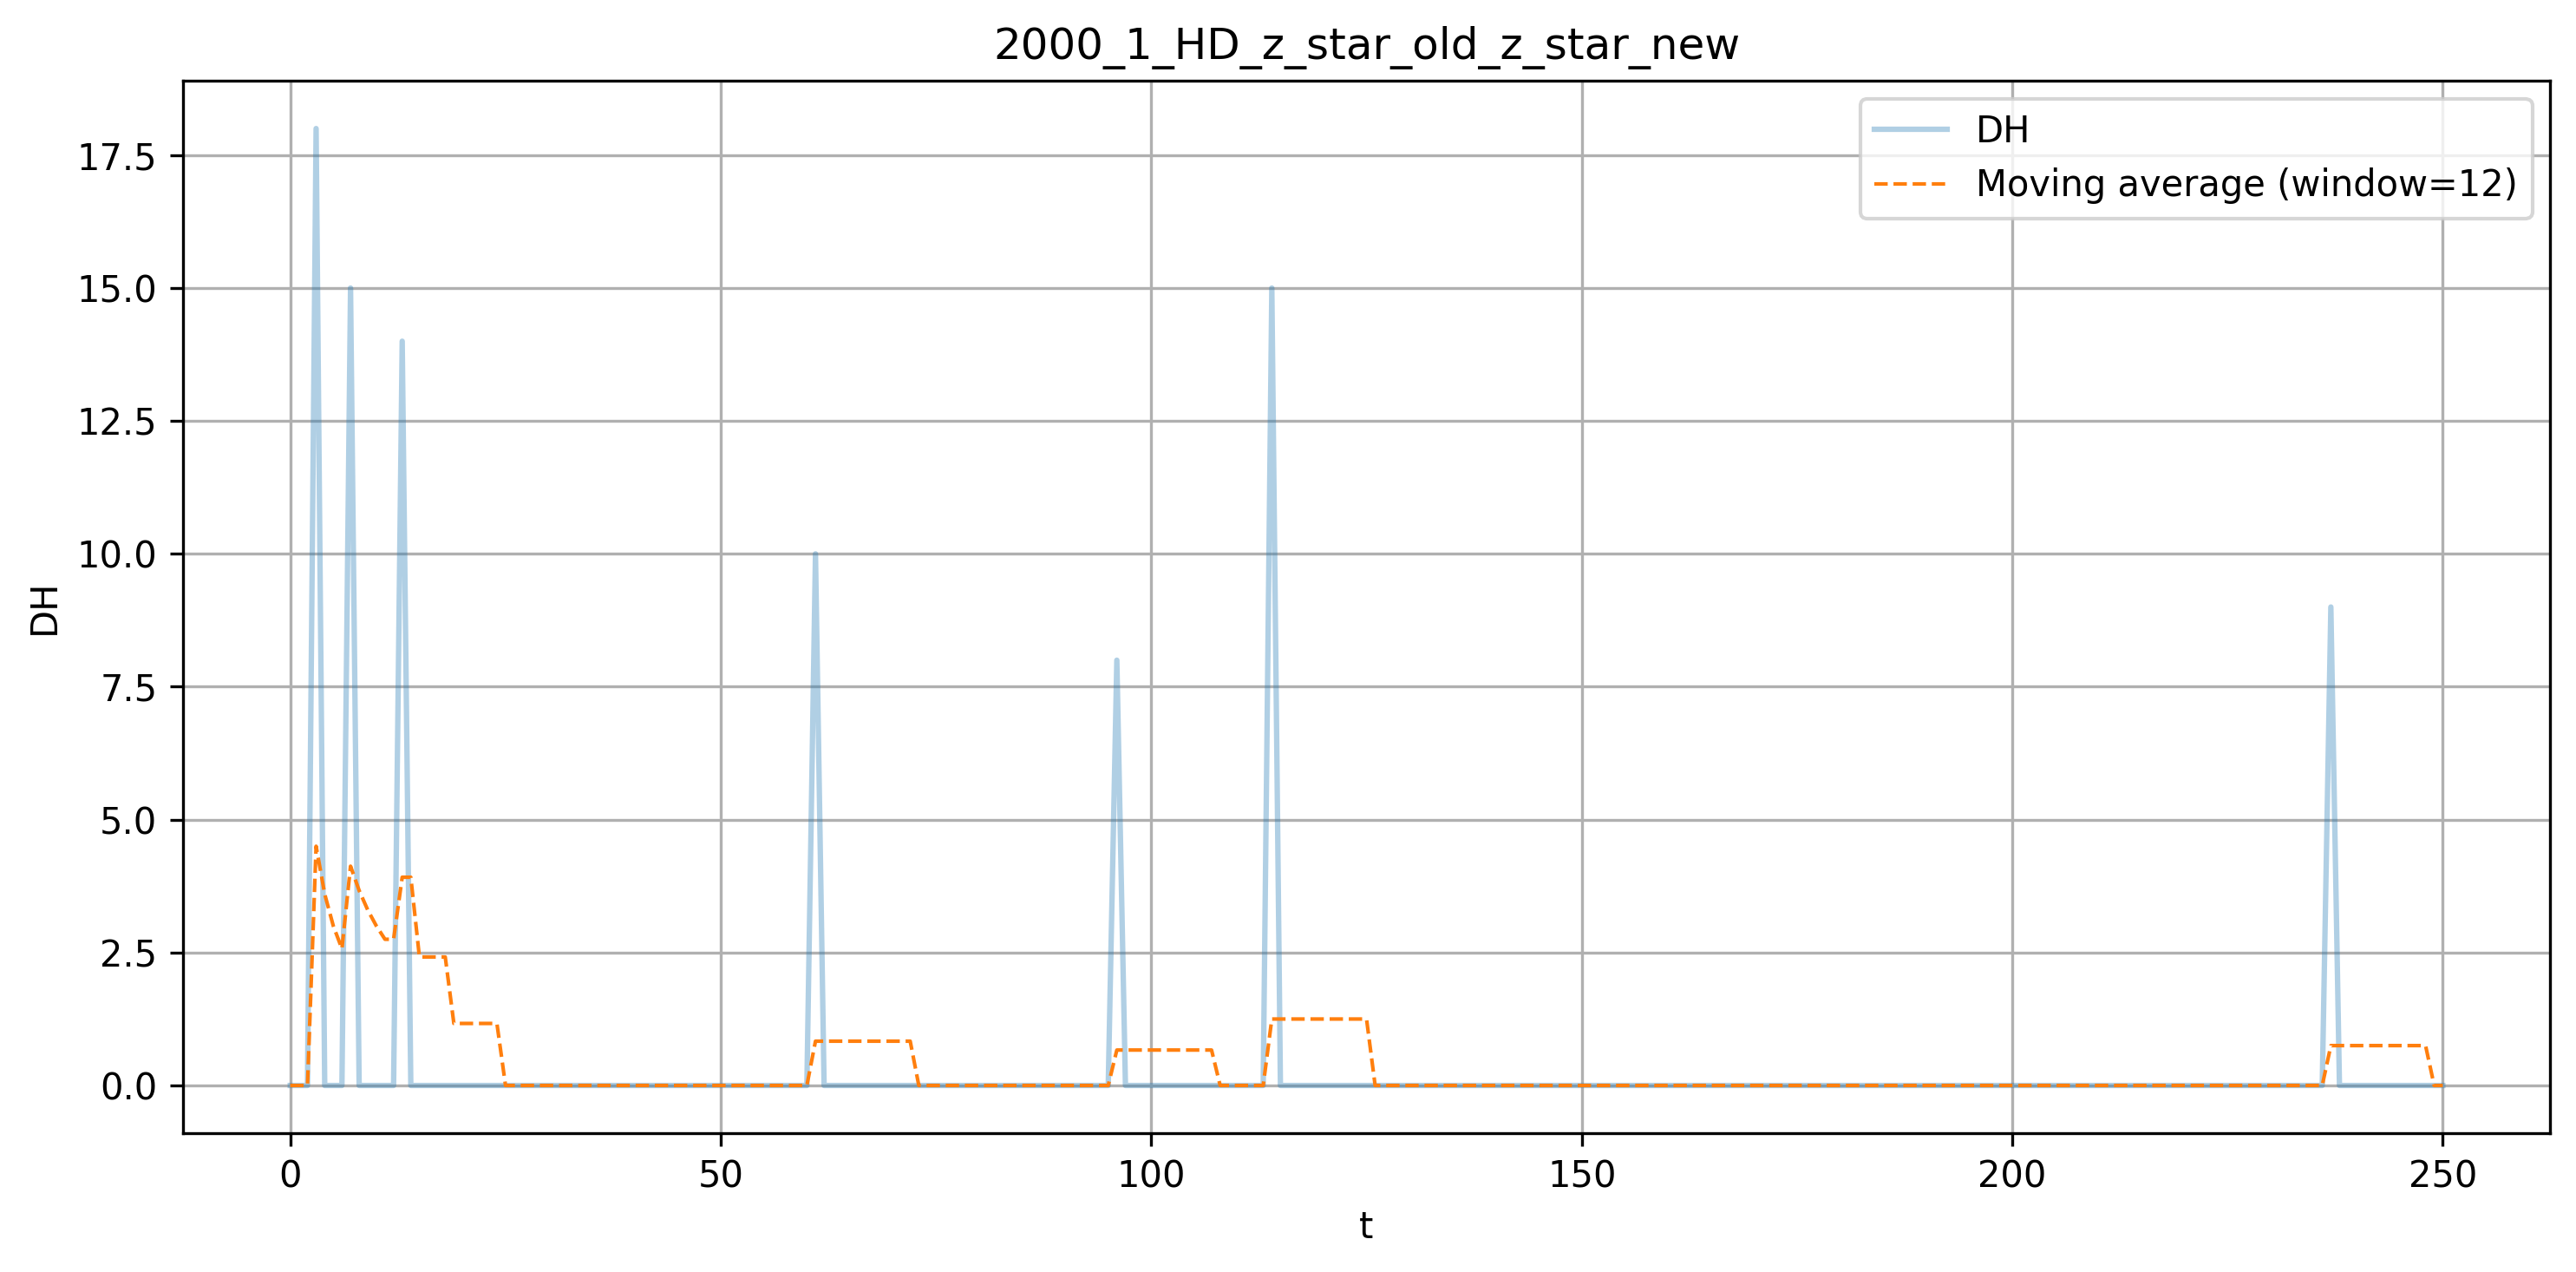
\includegraphics[width=\linewidth]{../Quantum-Annealing-for-solving-QUBO-Problems/test/Diagnostica_QALS/2/ksp_3/lambda_div_3/2000_1_HD_z_star_old_z_star_new.png}
    \caption{\(d_H(z_\star^{old}, z_\star^{new})\) con \(\lambda_2\)}
    \label{fig:hd-zstarold-zstarnew-lambda2}
\end{subfigure}
\hfill
\begin{subfigure}{0.495\textwidth}
    \centering
    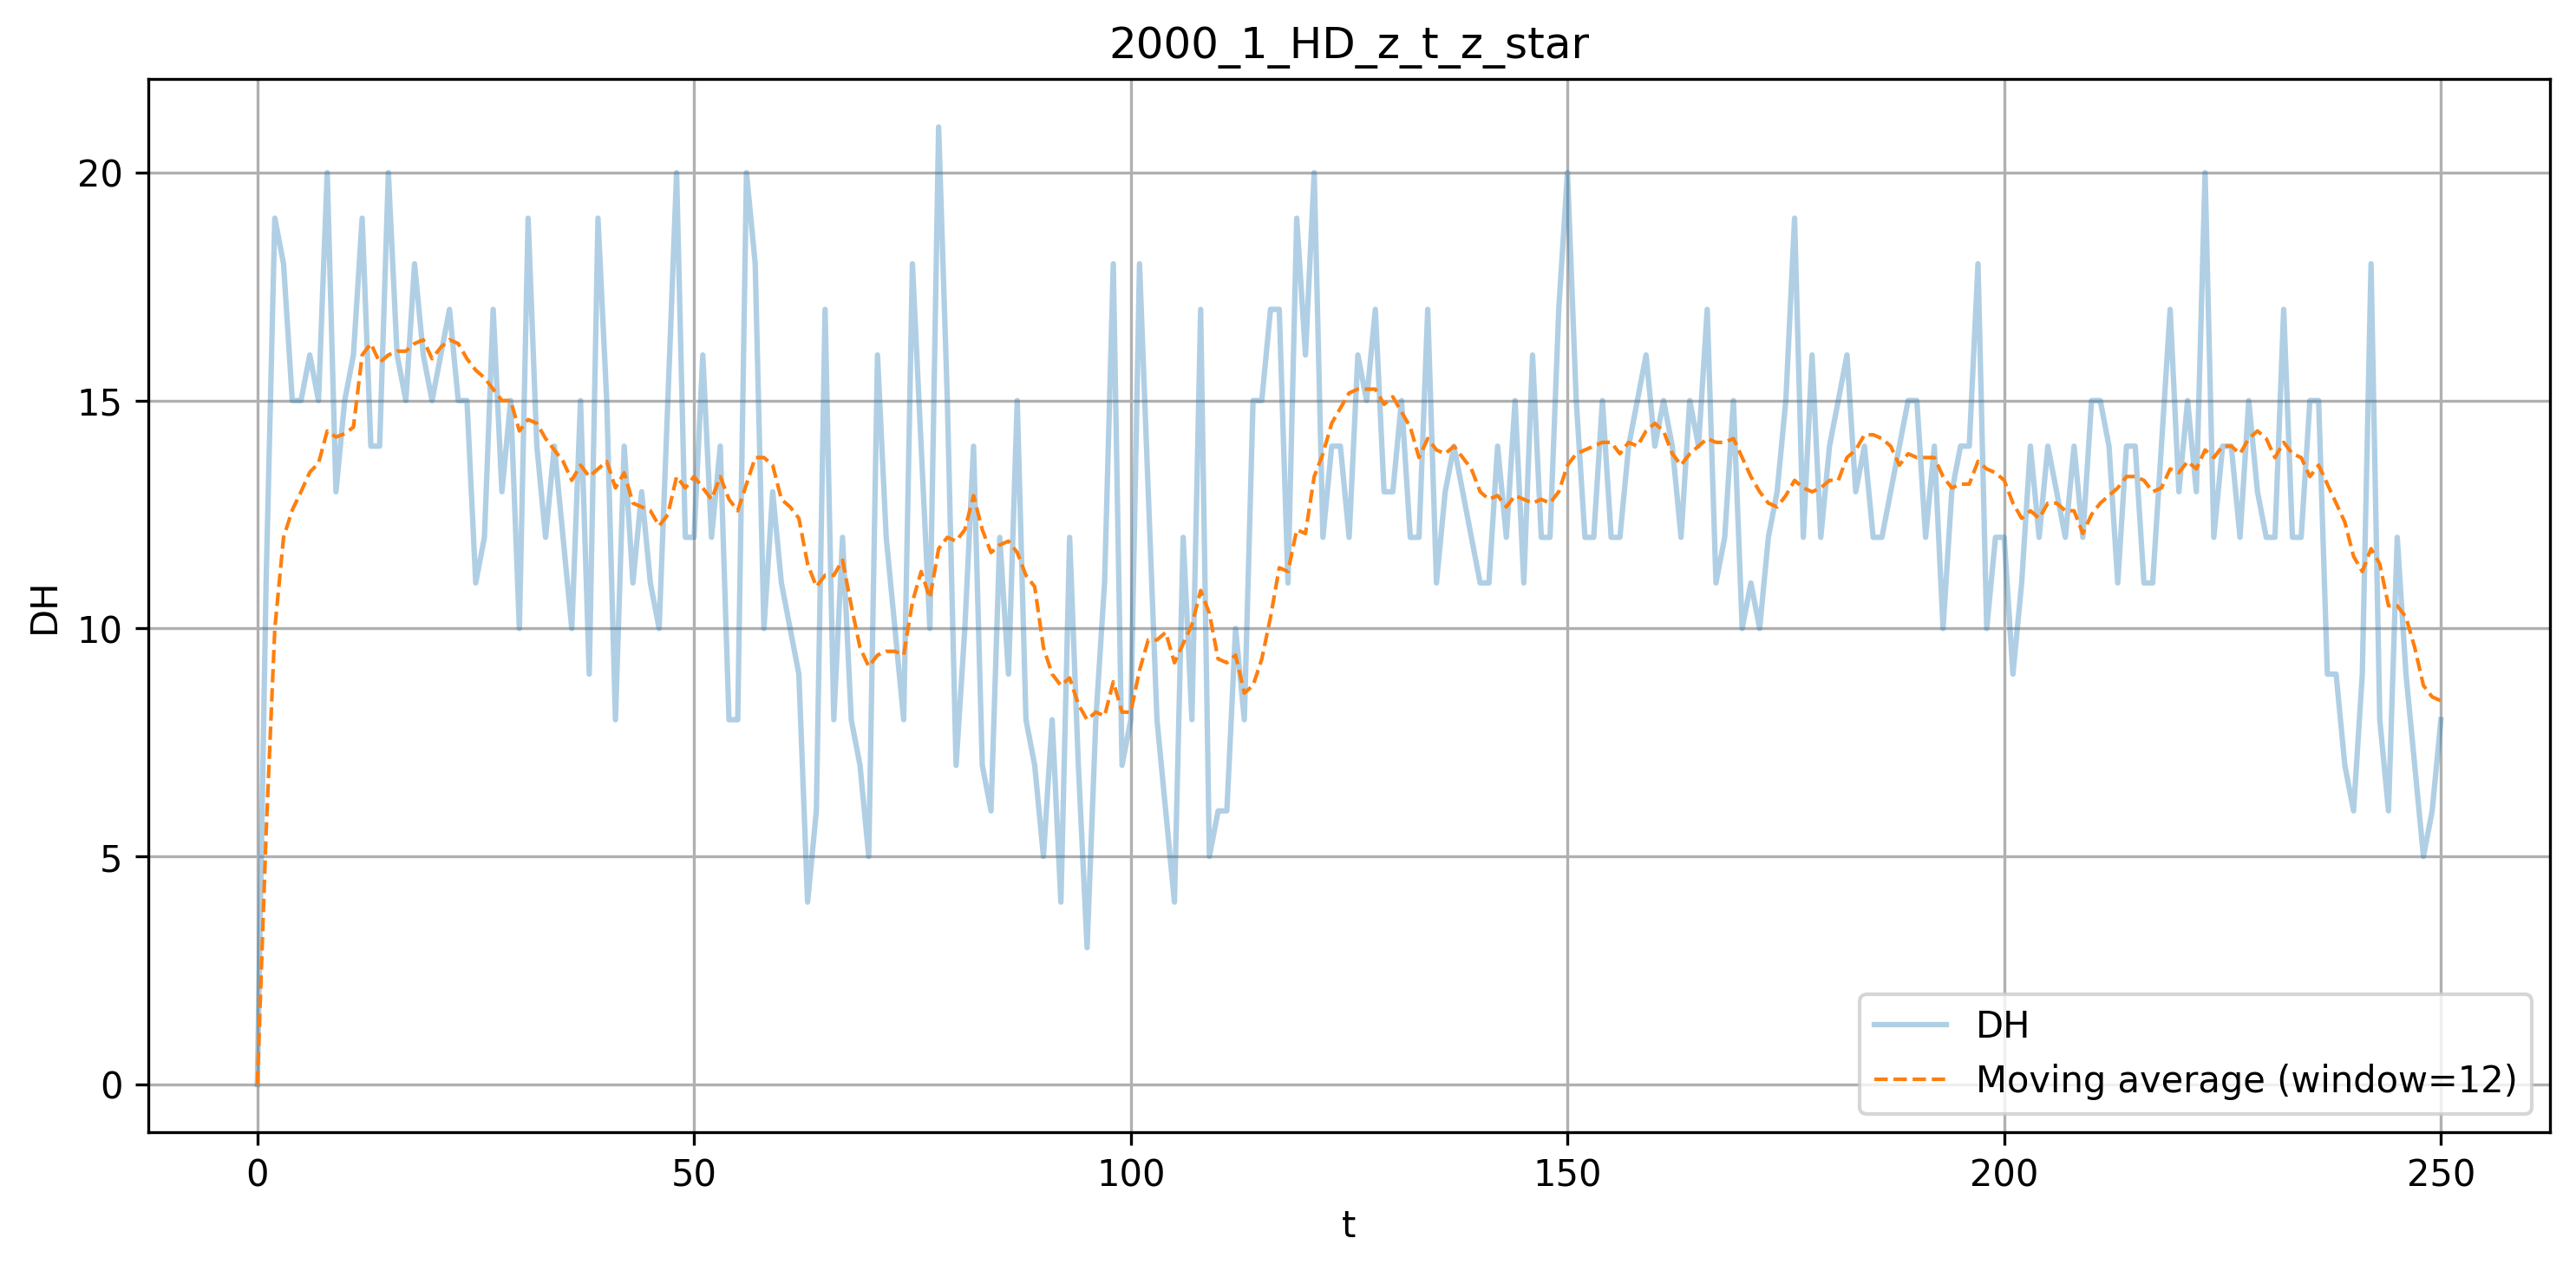
\includegraphics[width=\linewidth]{../Quantum-Annealing-for-solving-QUBO-Problems/test/Diagnostica_QALS/2/ksp_3/lambda_div_3/2000_1_HD_z_t_z_star.png}
    \caption{\(d_H(z_t, z_\star)\) con \(\lambda_2\)}
    \label{fig:hd-zt-zstar-lambda2}
\end{subfigure}

\vspace{0.35cm}

\begin{subfigure}{0.495\textwidth}
    \centering
    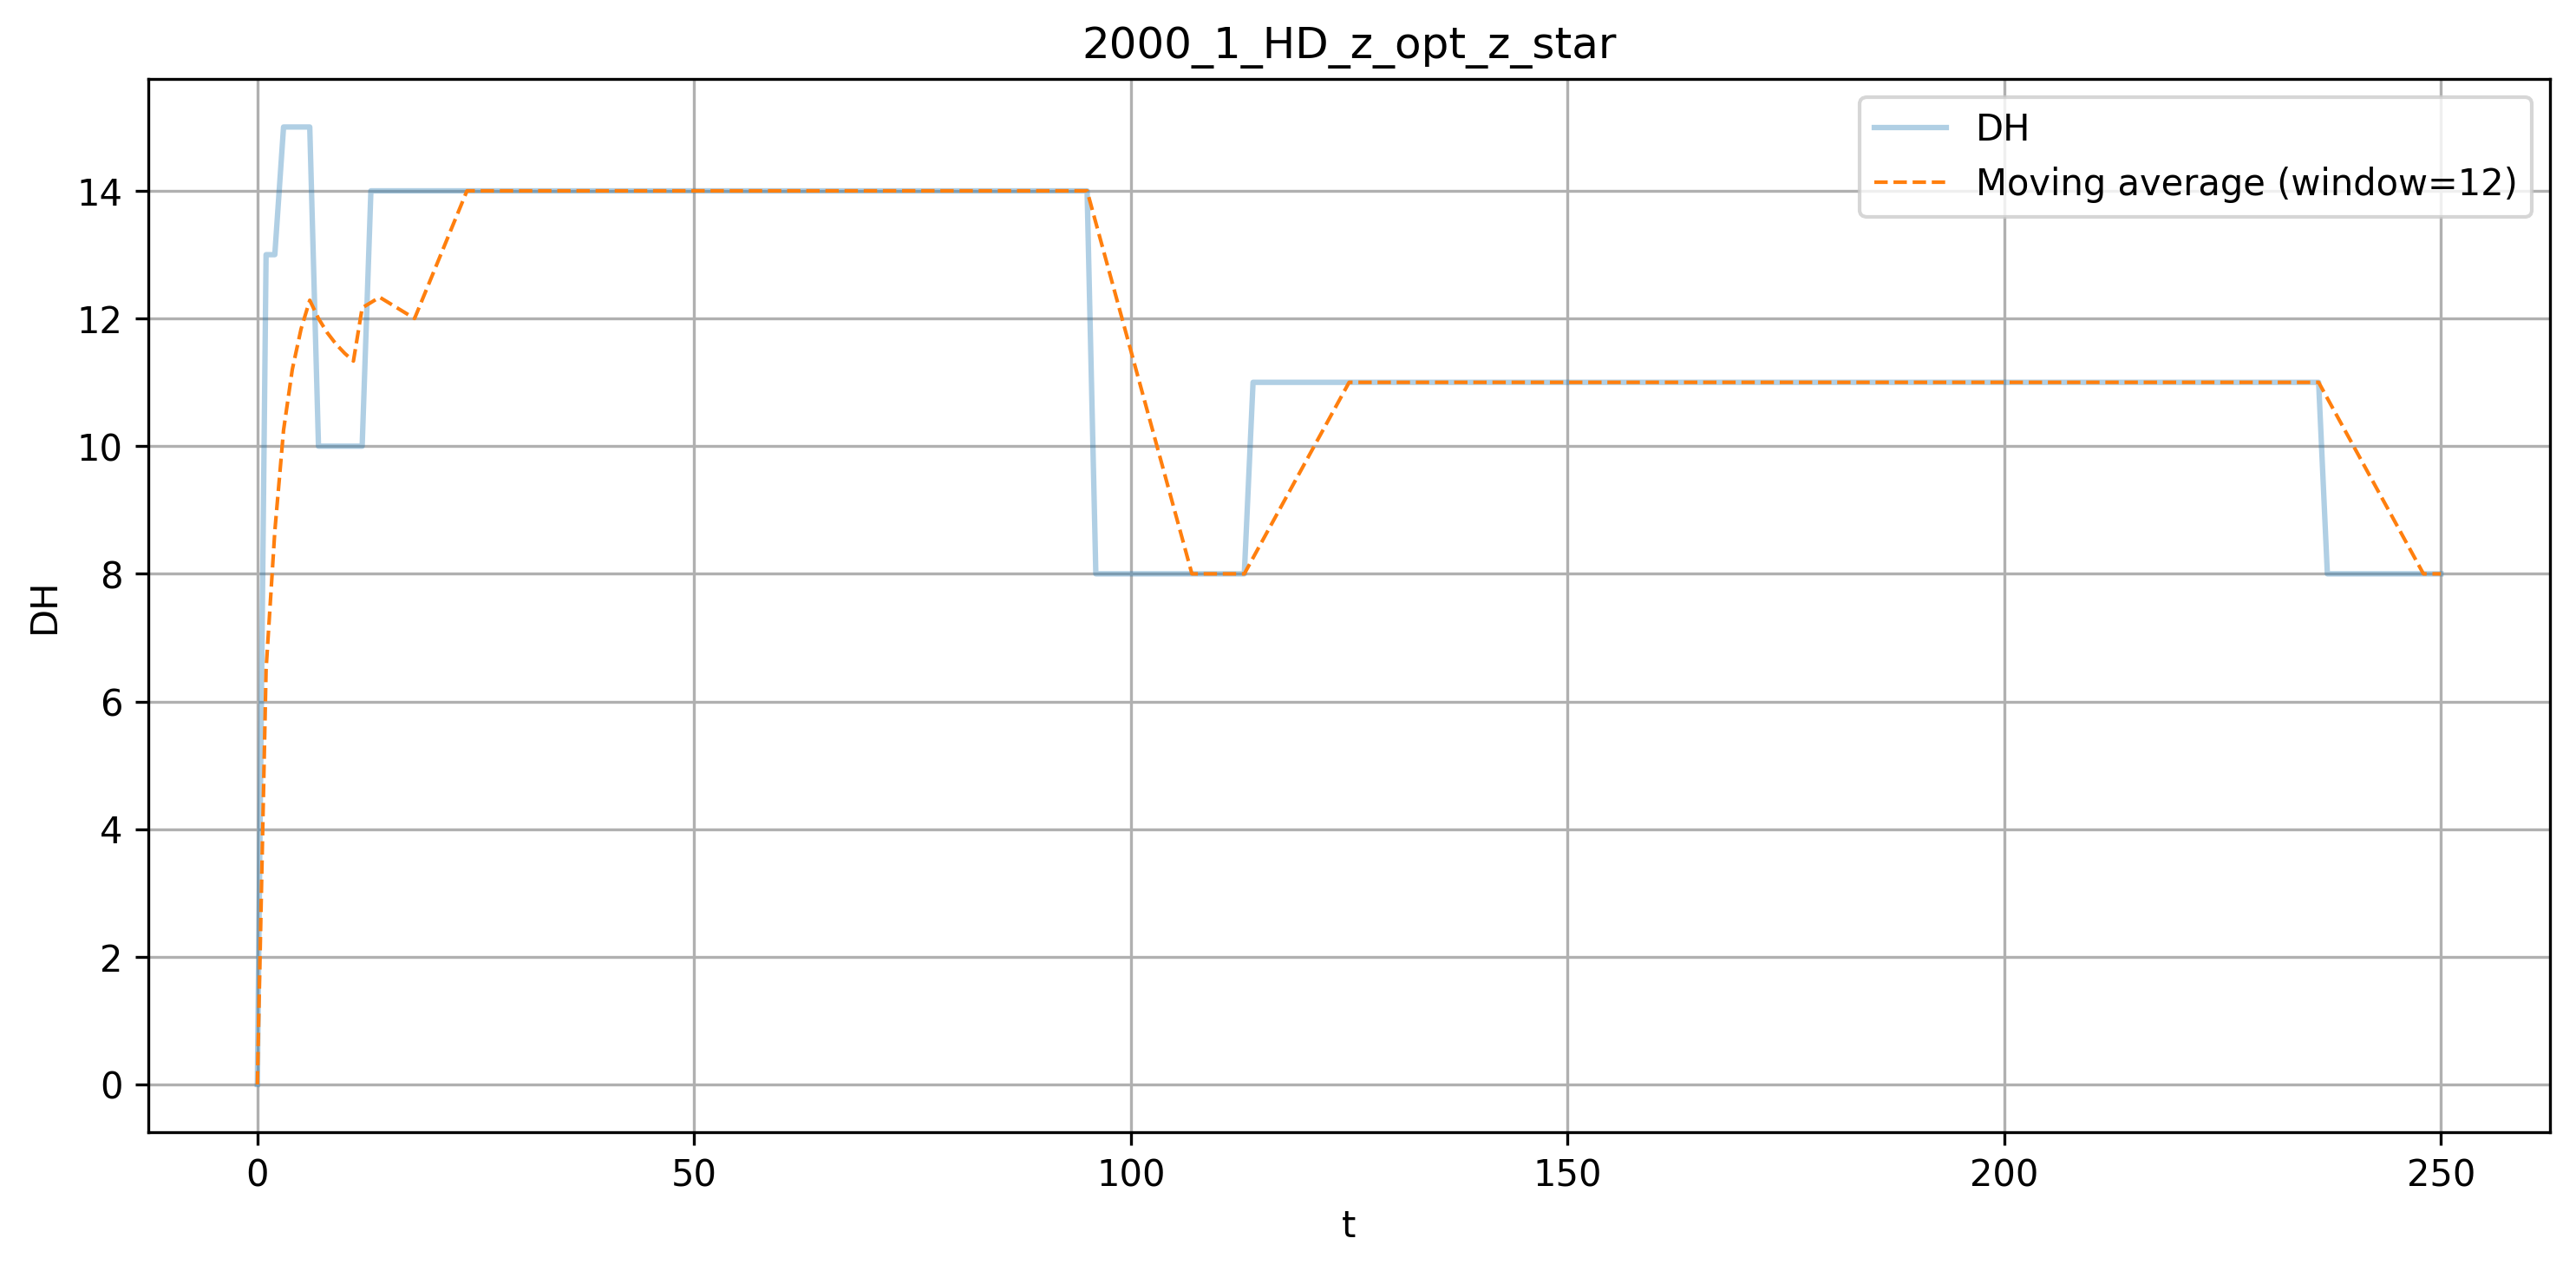
\includegraphics[width=\linewidth]{../Quantum-Annealing-for-solving-QUBO-Problems/test/Diagnostica_QALS/2/ksp_3/lambda_div_3/2000_1_HD_z_opt_z_star.png}
    \caption{\(d_H(z_{opt}, z_\star)\) con \(\lambda_2\)}
    \label{fig:hd-zopt-zstar-lambda2}
\end{subfigure}
\hfill
\begin{subfigure}{0.495\textwidth}
    \centering
    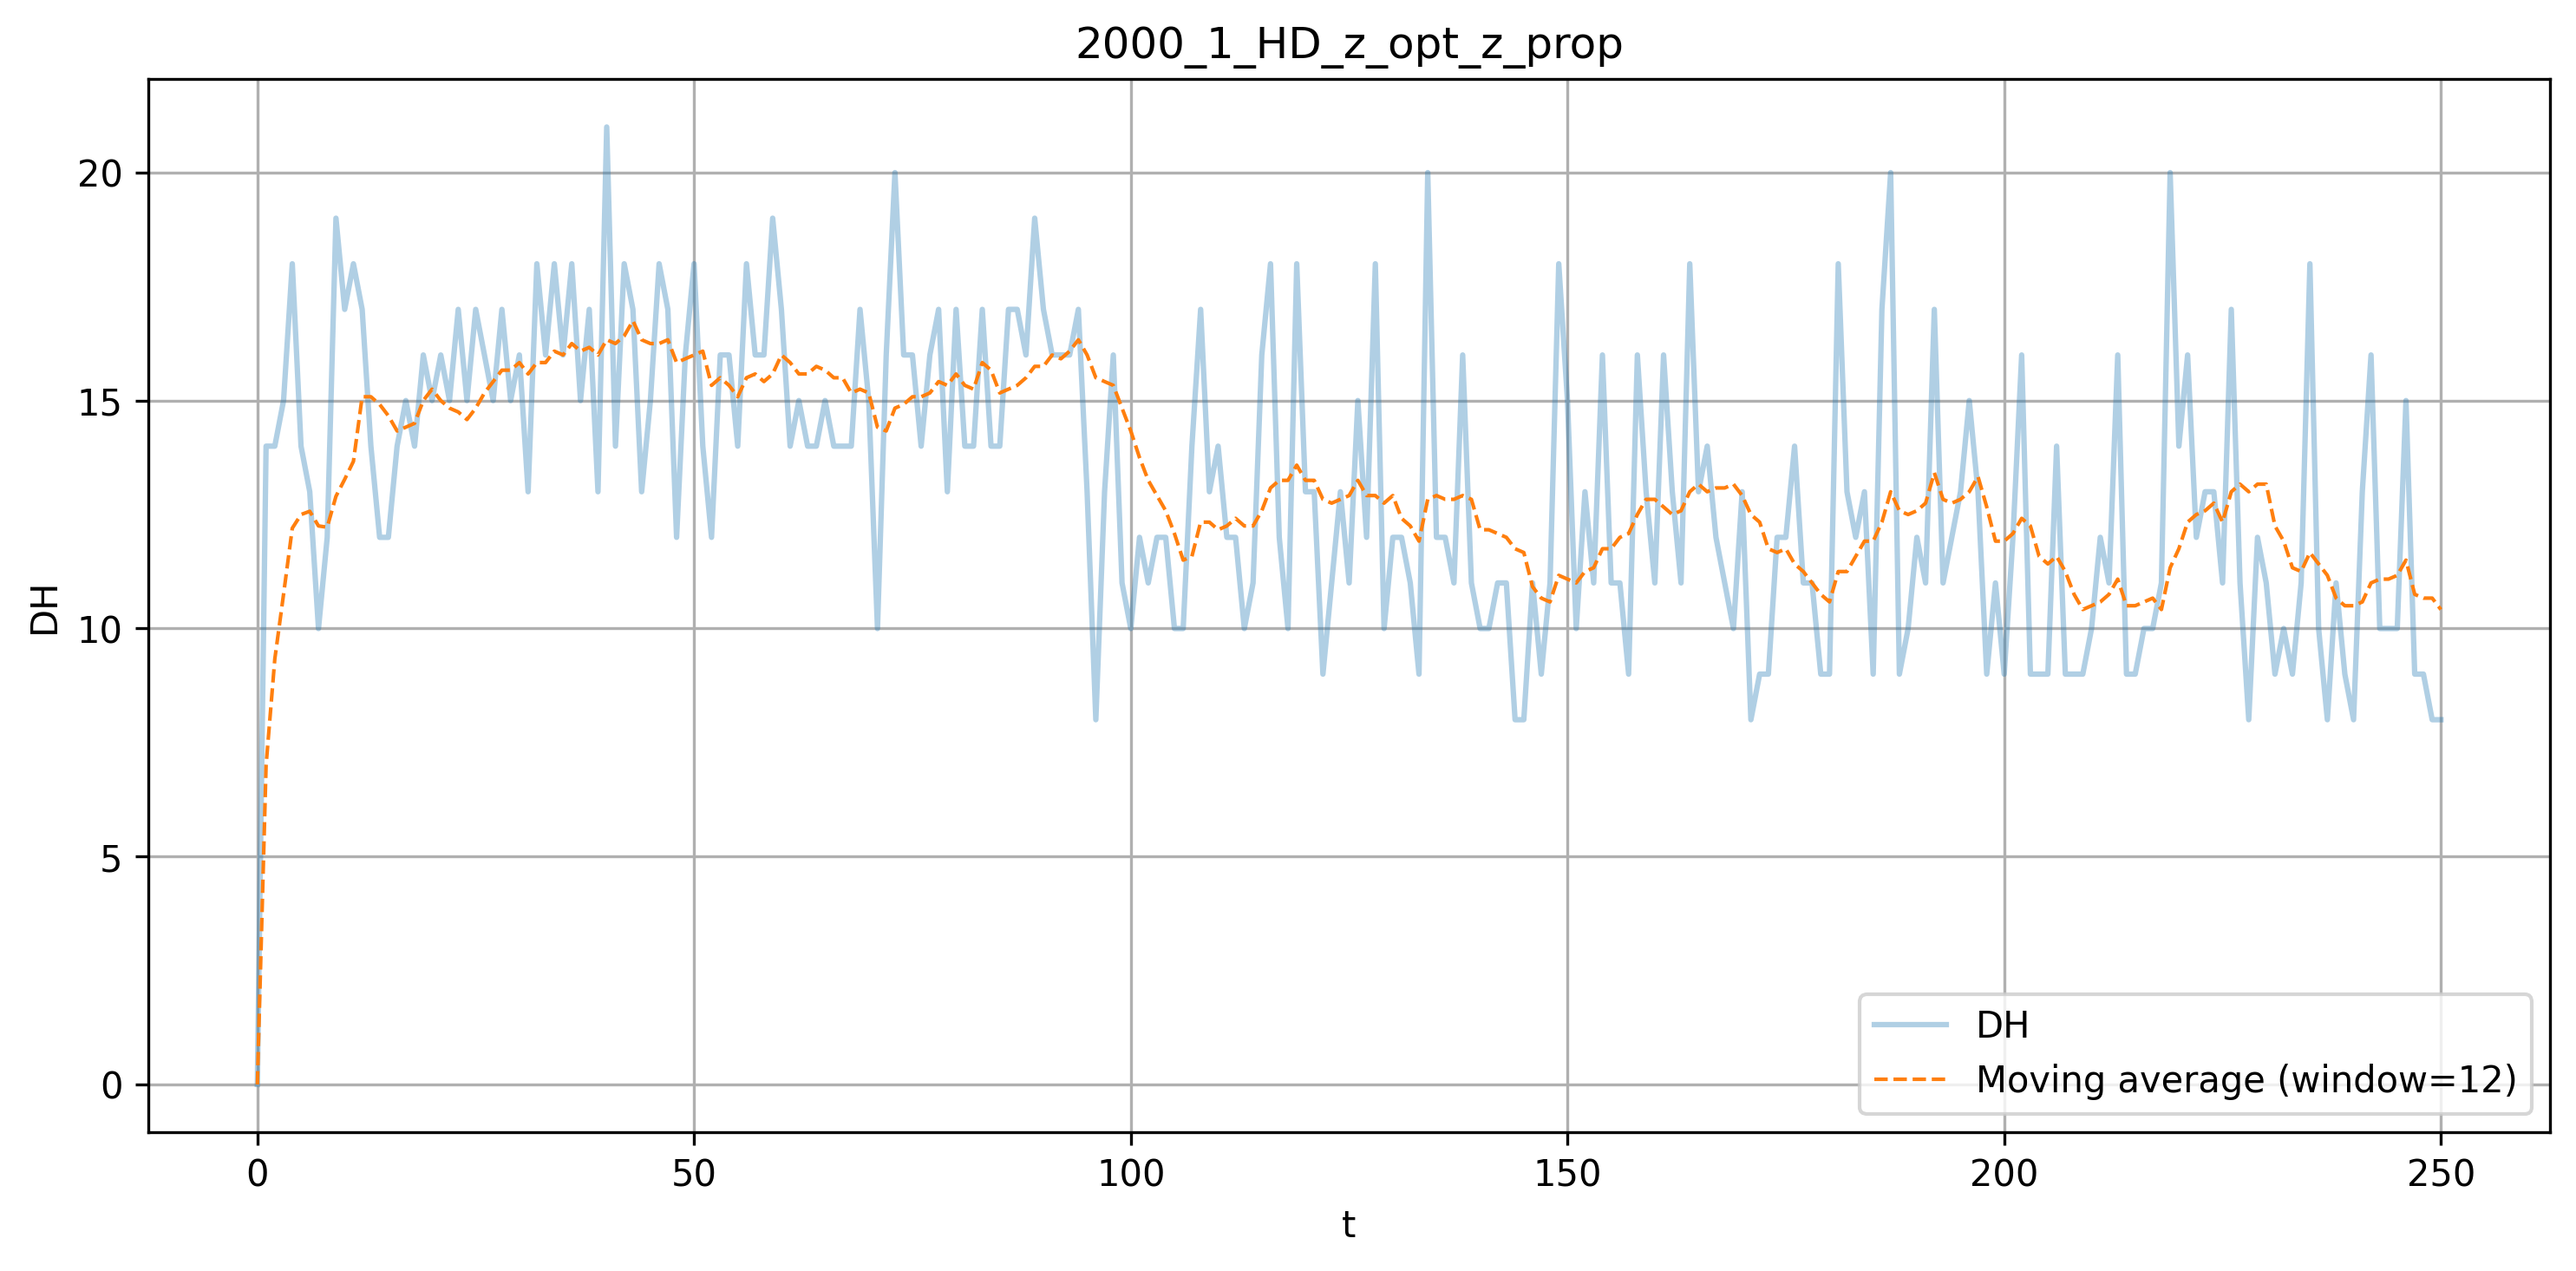
\includegraphics[width=\linewidth]{../Quantum-Annealing-for-solving-QUBO-Problems/test/Diagnostica_QALS/2/ksp_3/lambda_div_3/2000_1_HD_z_opt_z_prop.png}
    \caption{\(d_H(z_{opt}, z_t)\) con \(\lambda_2\)}
    \label{fig:hd-zopt-zt-lambda2}
\end{subfigure}

\vspace{0.35cm}

\begin{subfigure}{0.495\textwidth}
    \centering
    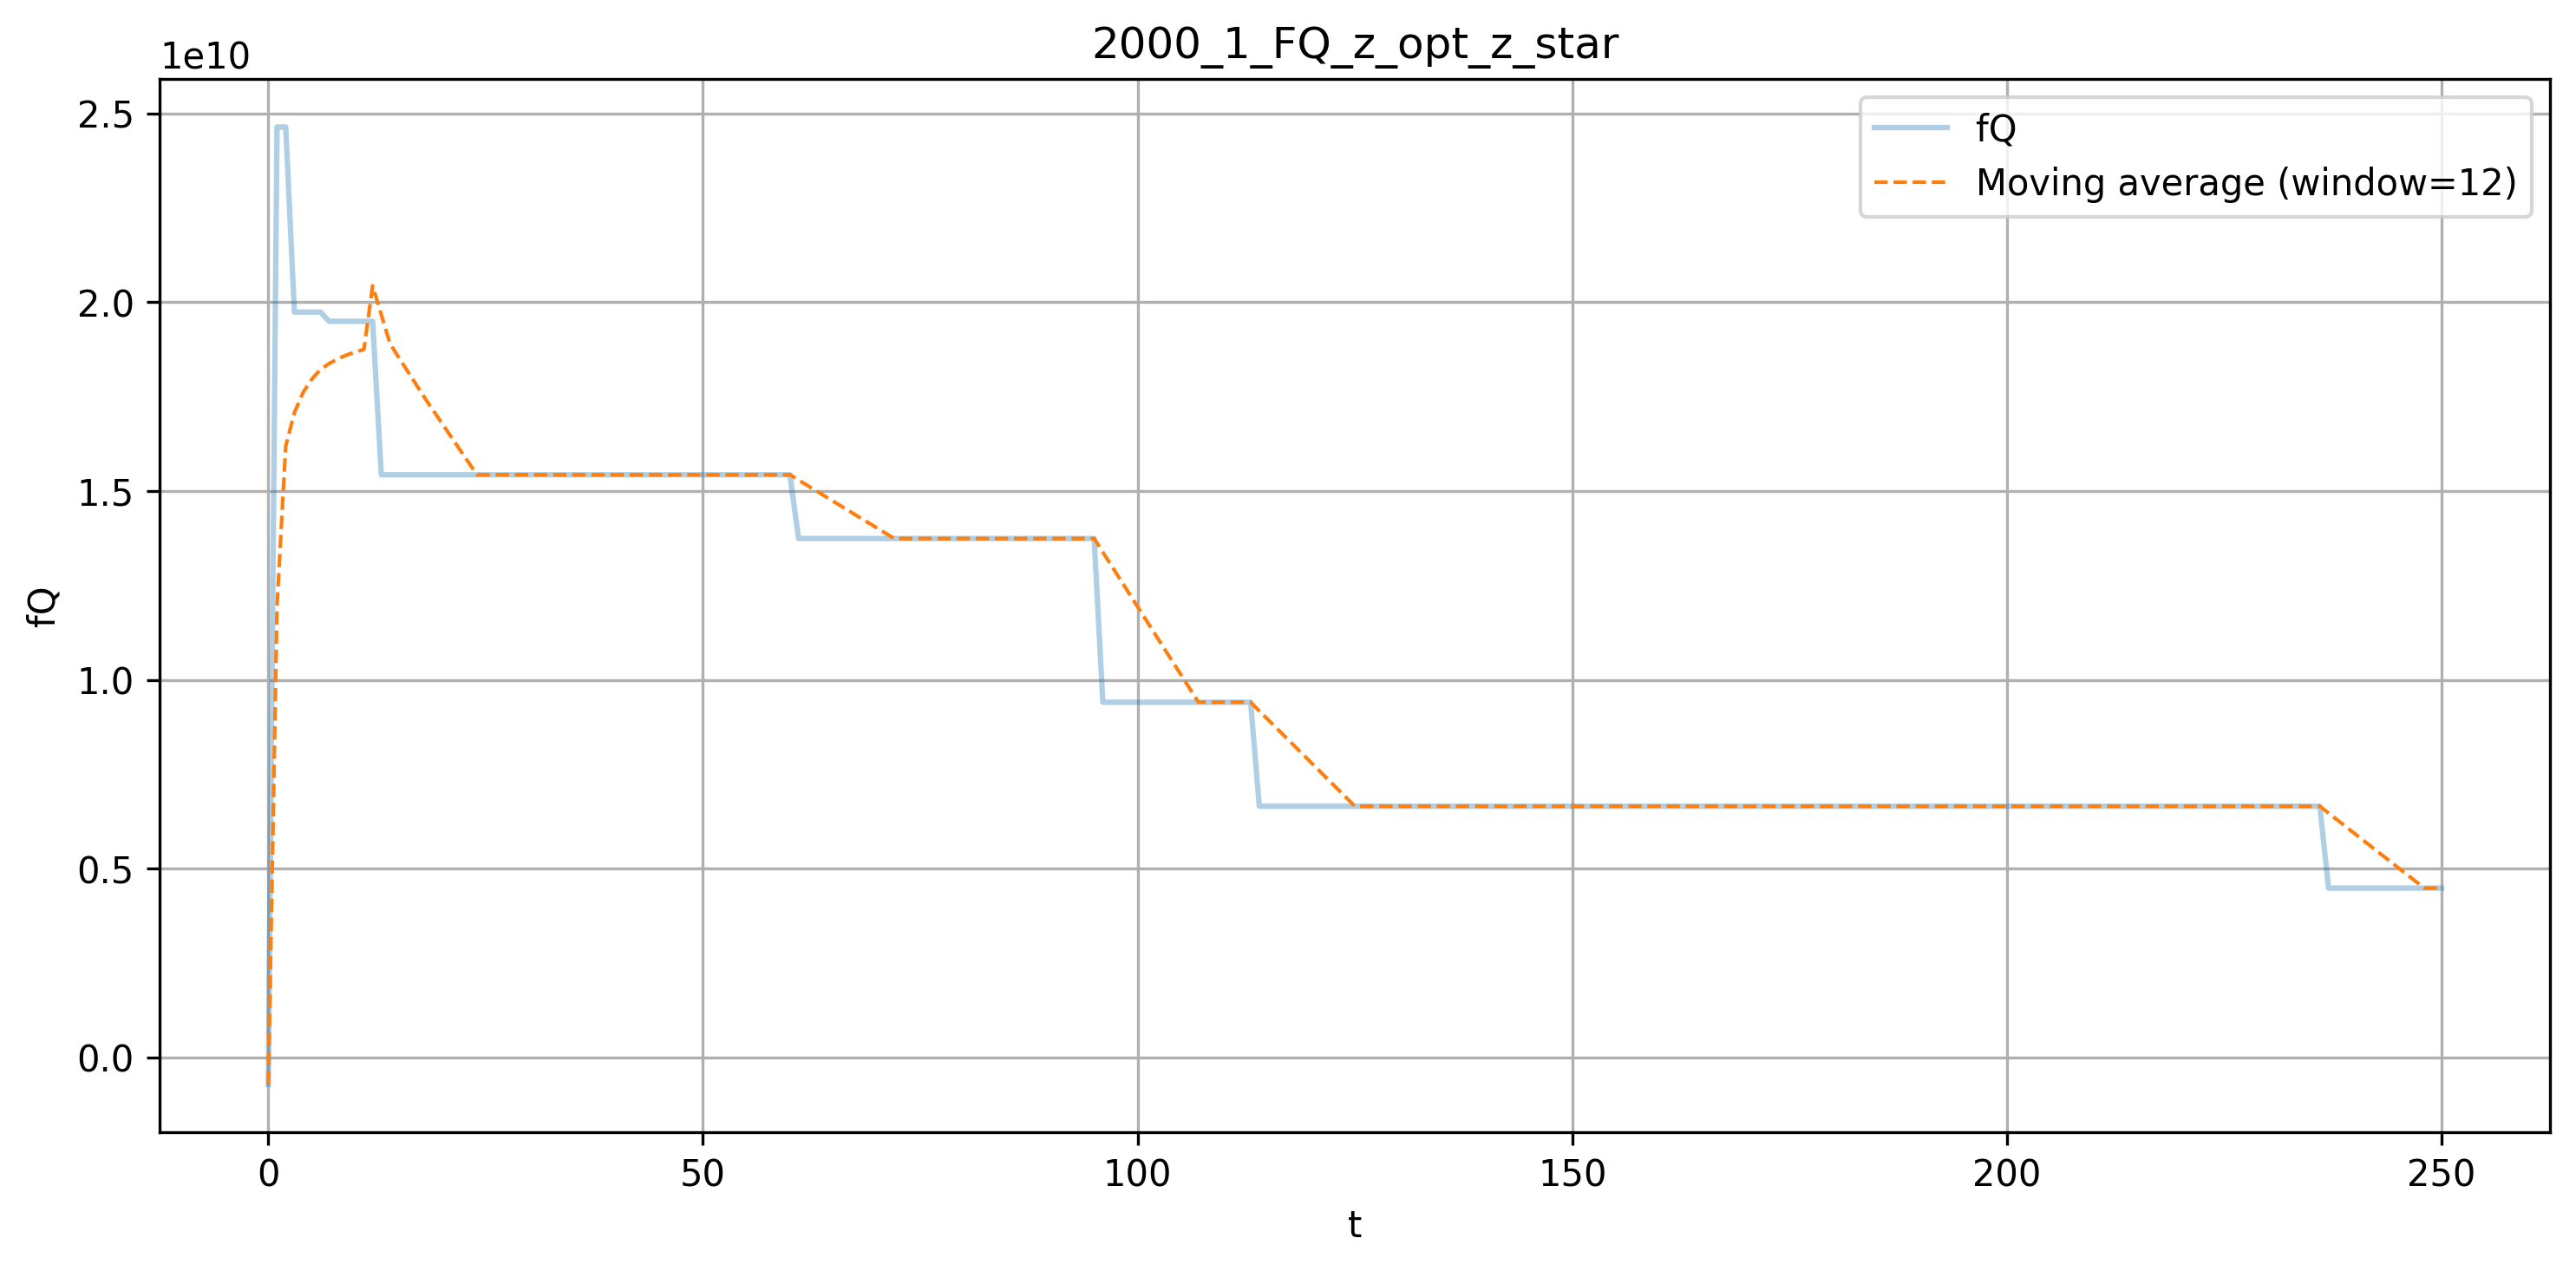
\includegraphics[width=\linewidth]{../Quantum-Annealing-for-solving-QUBO-Problems/test/Diagnostica_QALS/2/ksp_3/lambda_div_3/2000_1_FQ_z_opt_z_star.png}
    \caption{\(f_Q(z_\star)\) con \(\lambda_2\)}
    \label{fig:fQ-zstar-lambda2}
\end{subfigure}
\hfill
\begin{subfigure}{0.495\textwidth}
    \centering
    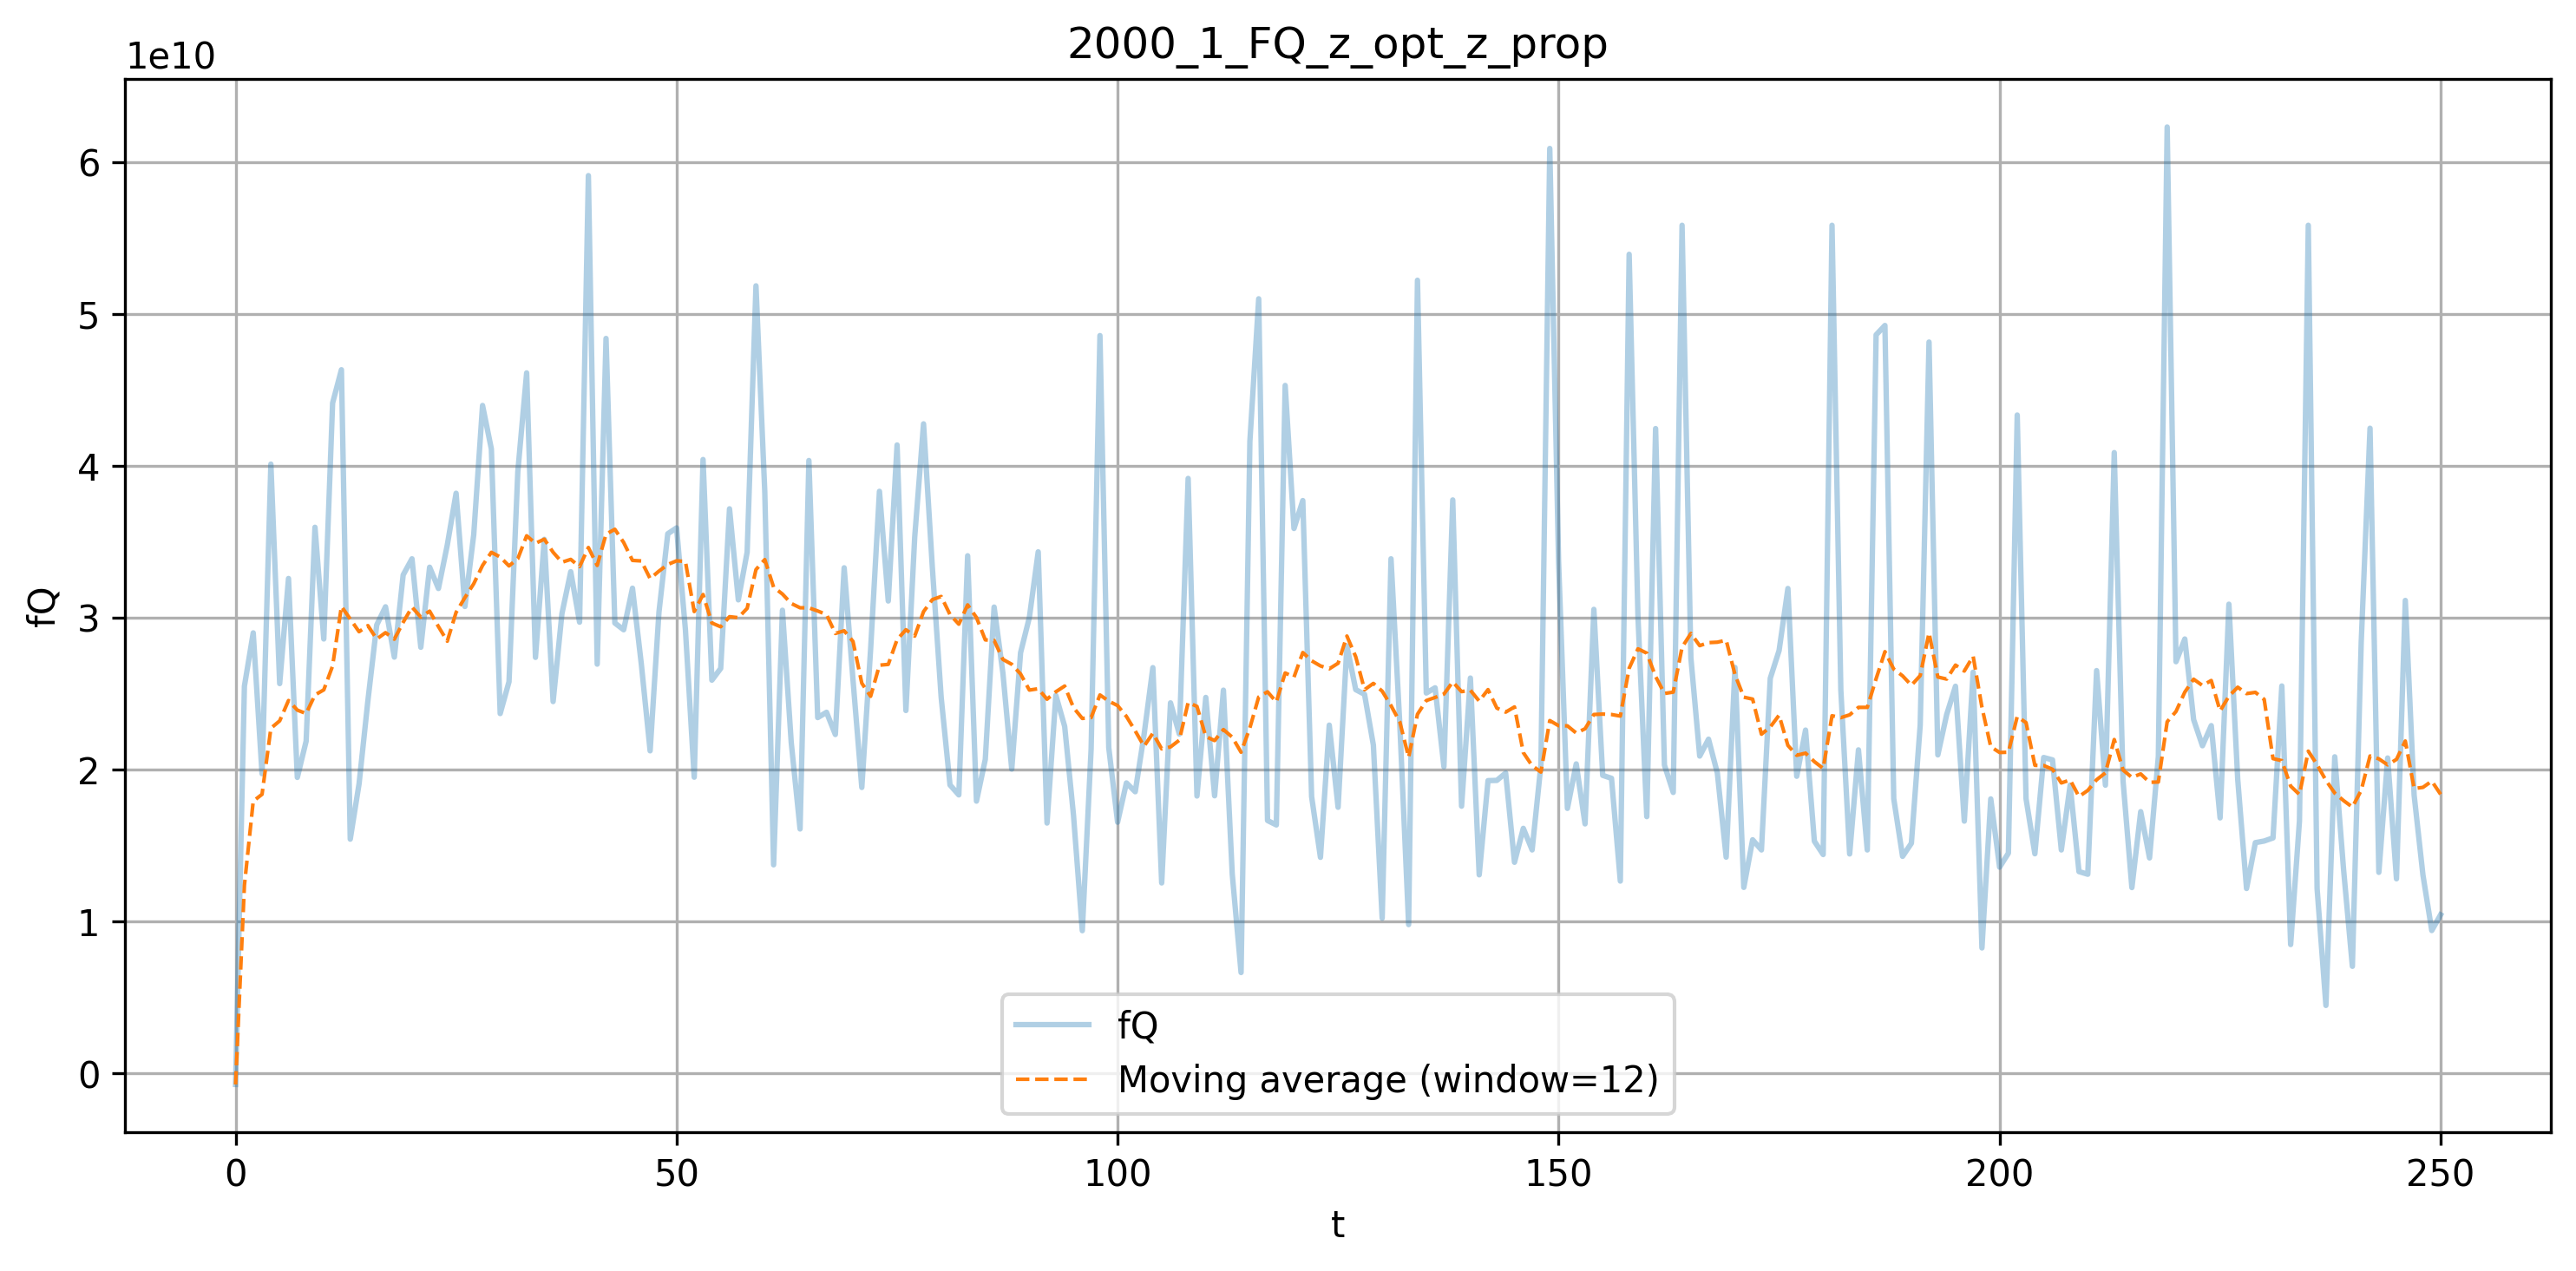
\includegraphics[width=\linewidth]{../Quantum-Annealing-for-solving-QUBO-Problems/test/Diagnostica_QALS/2/ksp_3/lambda_div_3/2000_1_FQ_z_opt_z_prop.png}
    \caption{\(f_Q(z_t)\) con \(\lambda_2\)}
    \label{fig:fQ-zt-lambda2}
\end{subfigure}
\label{fig:confronto-hamming-ksp32}
\end{figure}

\begin{figure}[H]
\centering
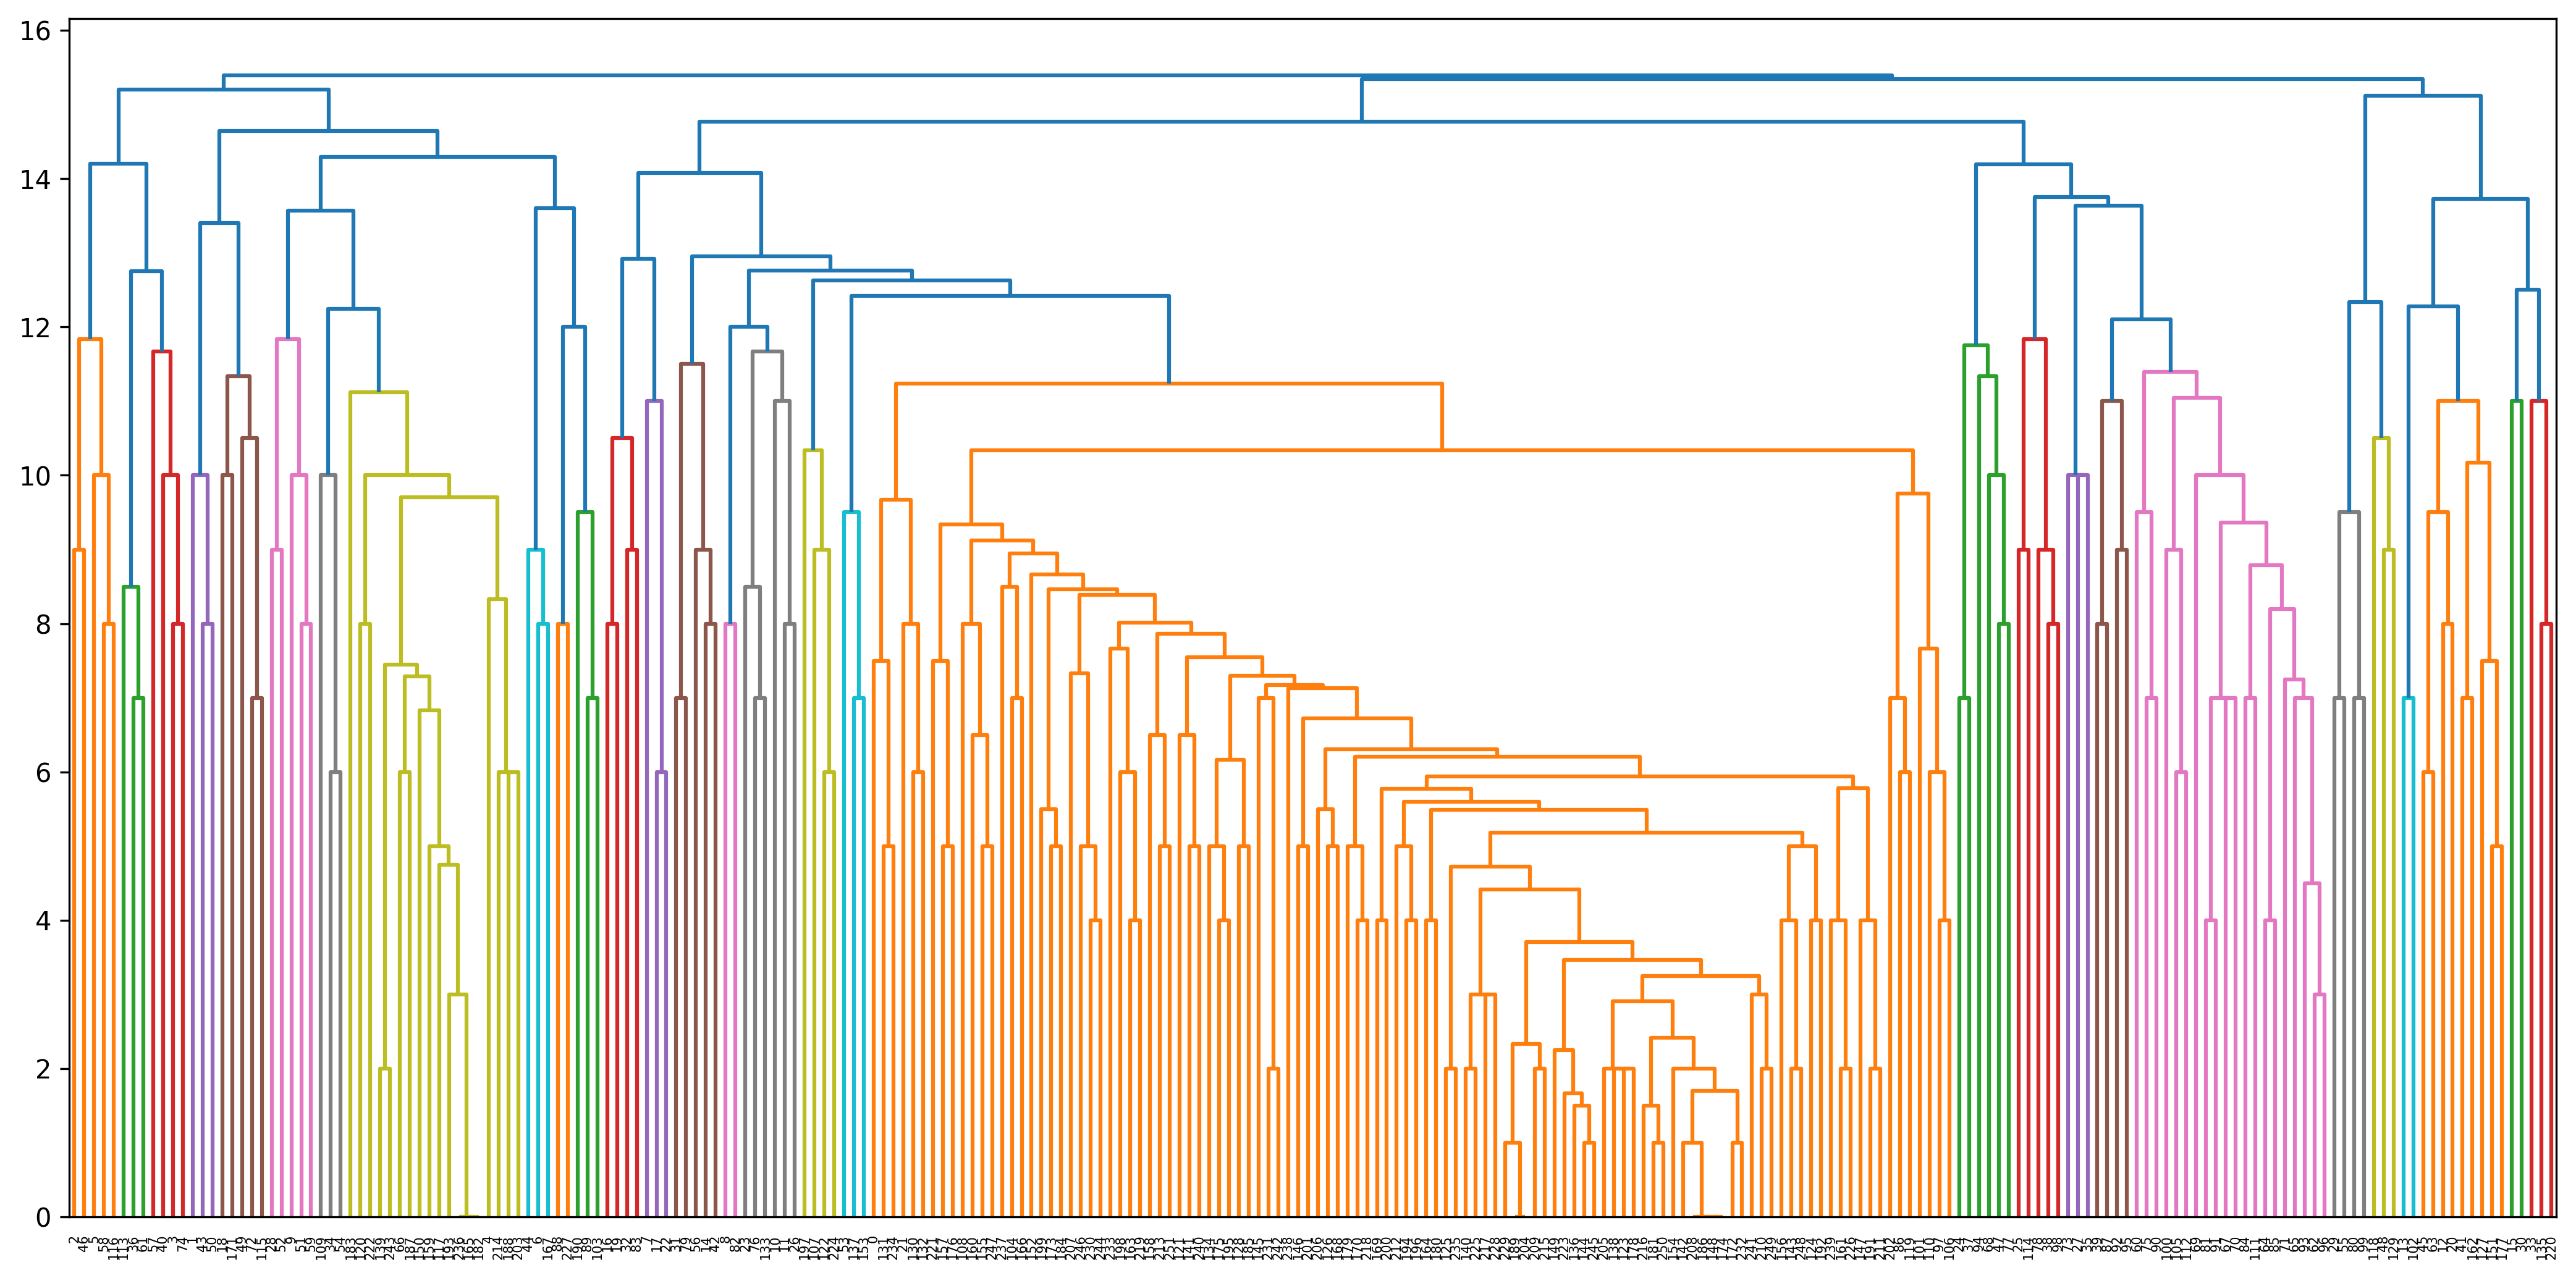
\includegraphics[width=\linewidth]{../Quantum-Annealing-for-solving-QUBO-Problems/test/Diagnostica_QALS/2/ksp_3/lambda_div_3/dendrogram_2000_1.png}
\caption{Agglomerative Clustering Dendogram}
\label{fig:AgglomerativeClustering-ksp3}
\end{figure}

\clearpage
\subsection{ksp\_2}

\begin{table}[h]
\centering
\begin{tabular}{lcc}
\hline
\textbf{Metrica} & \(\lambda_1\) & \(\lambda_2\) \\
\hline
Numero cluster & 46 & 47 \\
Dimensione cluster massimo & 90 & 68 \\
Cluster z best & 0 & 26 \\
Single clusters & 5 & 3 \\
\(f_Q\) medoid & 8491845.63 & 1813962265458.67 \\
Profit medoid & 18328 & 17973 \\
Weight medoid & 14503 & 14387 \\
\hline
\(f_Q\) Min Found QALS & 828636.47 & 496218019323.67 \\
Profit Found QALS & 10497 & 13719 \\
Weight Found QALS & 5346 & 8054 \\
\hline
\(f_Q\) Min Found NO QALS & -54748.31 & -10200709849.33 \\
Profit Found NO QALS & 7740 & 5669 \\
Weight Found NO QALS & 978 & 1001 \\
\hline
\end{tabular}

\caption{Confronto dei risultati ottenuti con QALS e senza QALS.}
\label{tab:confronto-qals-noqals}
\end{table}

\begin{figure}[H]
\centering
\begin{subfigure}{0.495\textwidth}
    \centering
    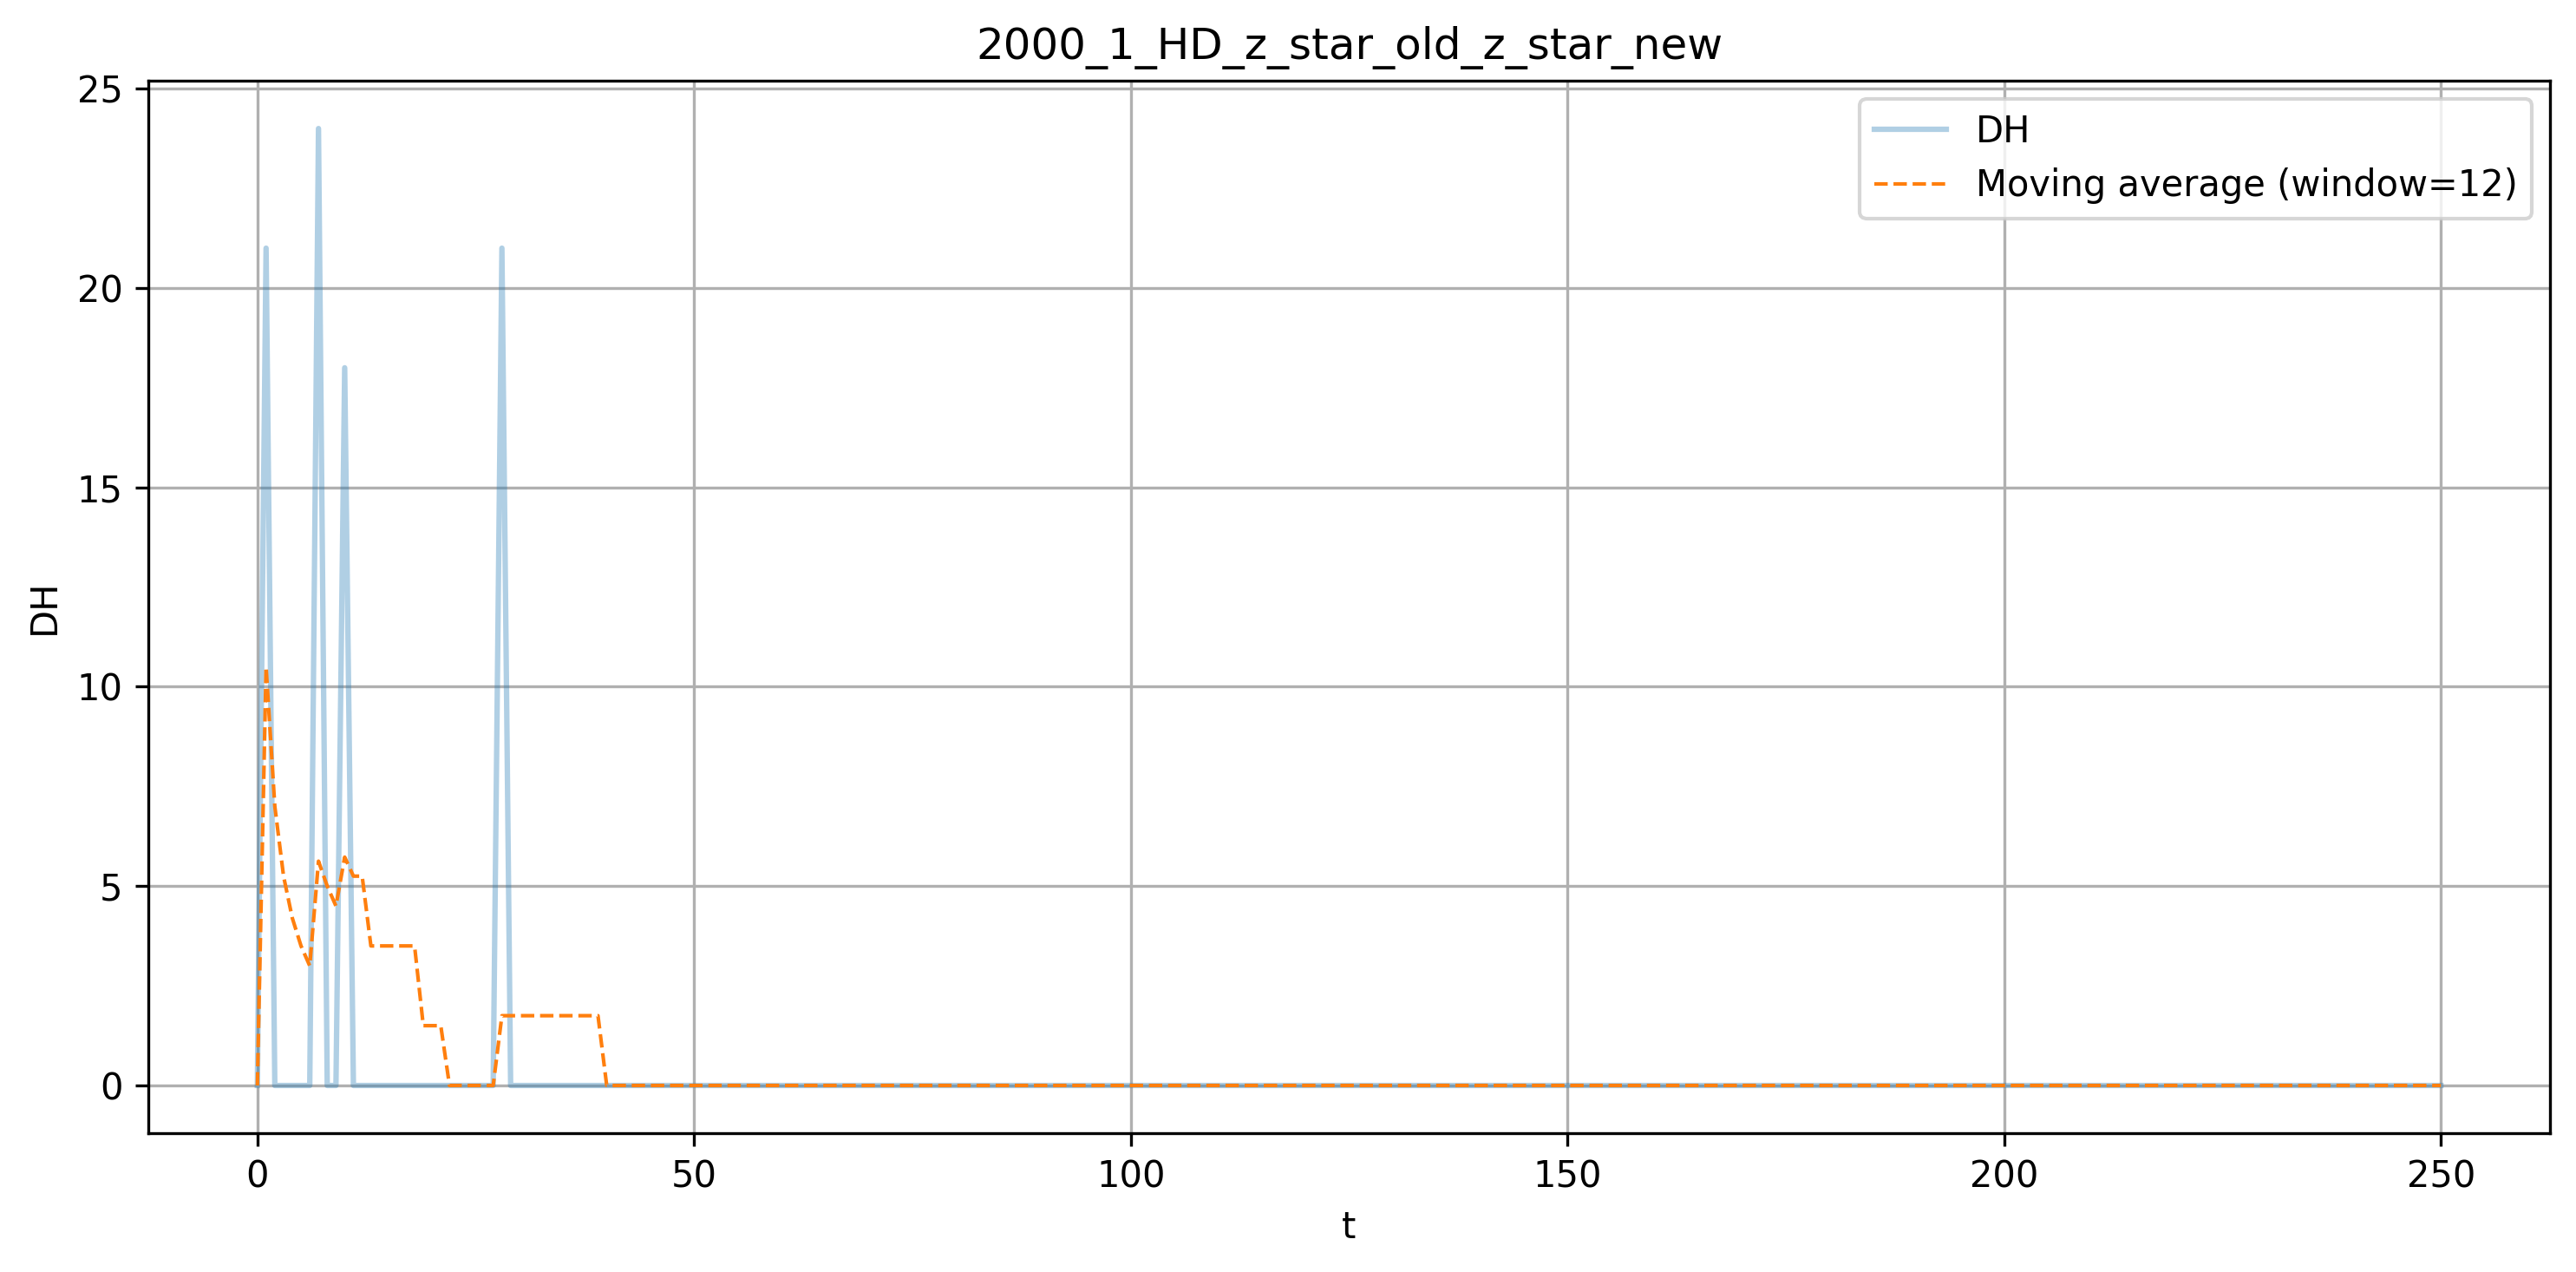
\includegraphics[width=\linewidth]{../Quantum-Annealing-for-solving-QUBO-Problems/test/Diagnostica_QALS/2/ksp_2/lambda_650_dot_C/2000_1_HD_z_star_old_z_star_new.png}
    \caption{\(d_H(z_\star^{old}, z_\star^{new})\) con \(\lambda_1\)}
    \label{fig:hd-zstarold-zstarnew-lambda1}
\end{subfigure}
\hfill
\begin{subfigure}{0.495\textwidth}
    \centering
    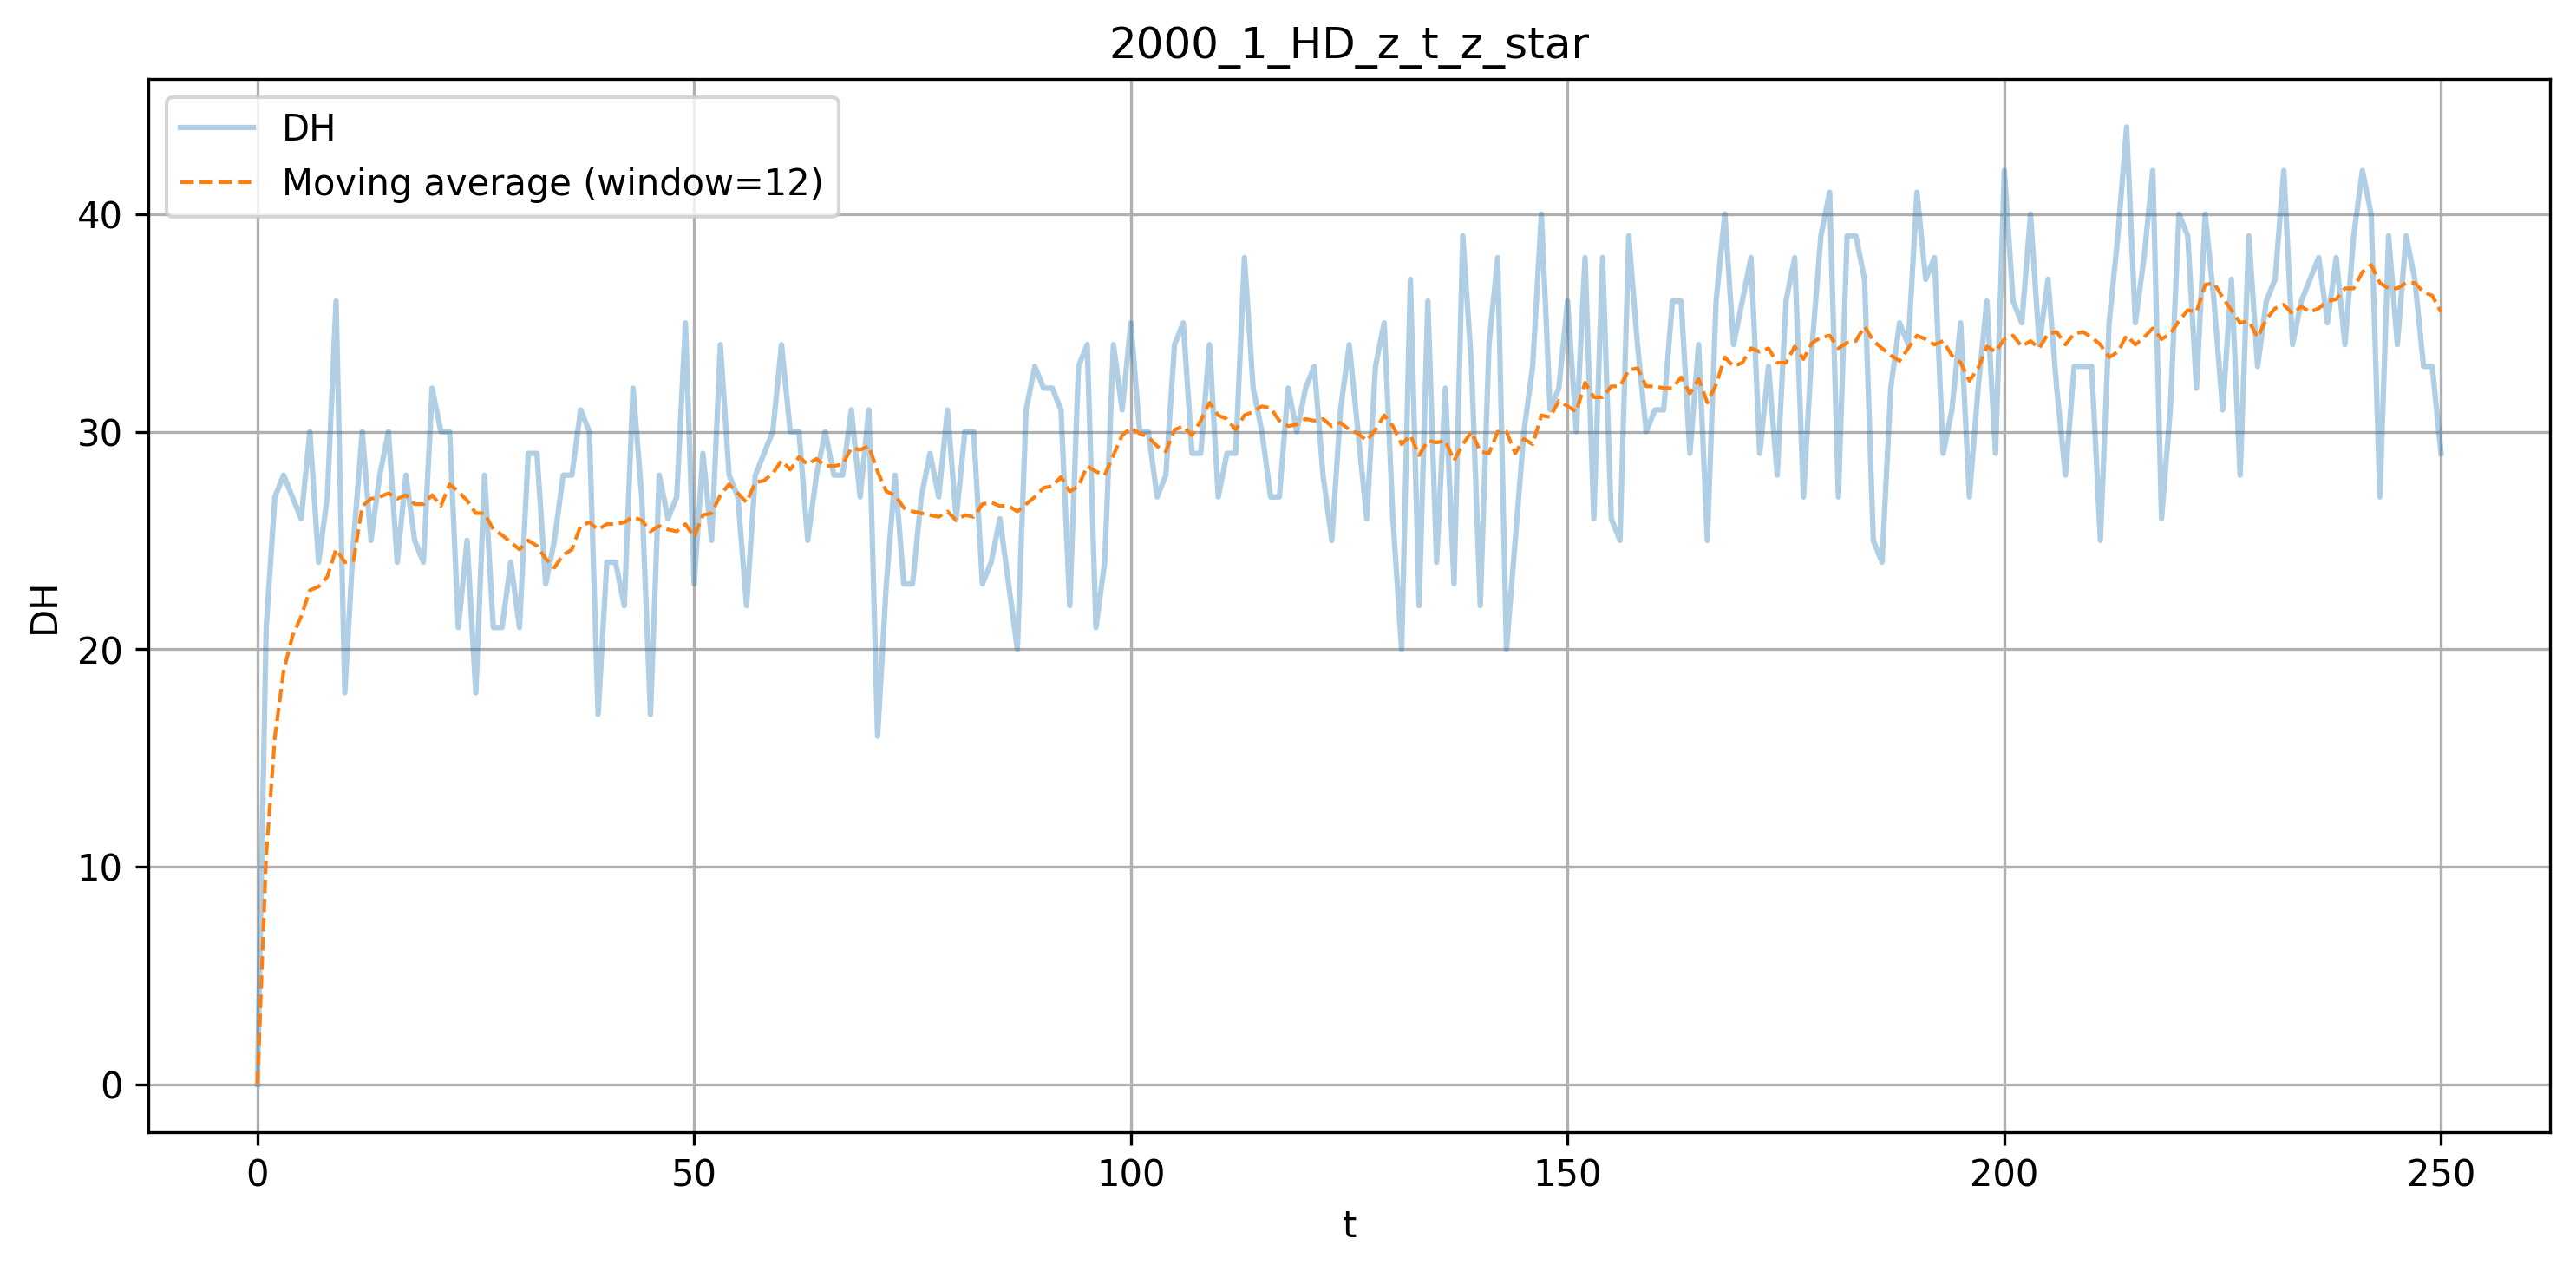
\includegraphics[width=\linewidth]{../Quantum-Annealing-for-solving-QUBO-Problems/test/Diagnostica_QALS/2/ksp_2/lambda_650_dot_C/2000_1_HD_z_t_z_star.png}
    \caption{\(d_H(z_t, z_\star)\) con \(\lambda_1\)}
    \label{fig:hd-zt-zstar-lambda1}
\end{subfigure}

\vspace{0.35cm}

\begin{subfigure}{0.495\textwidth}
    \centering
    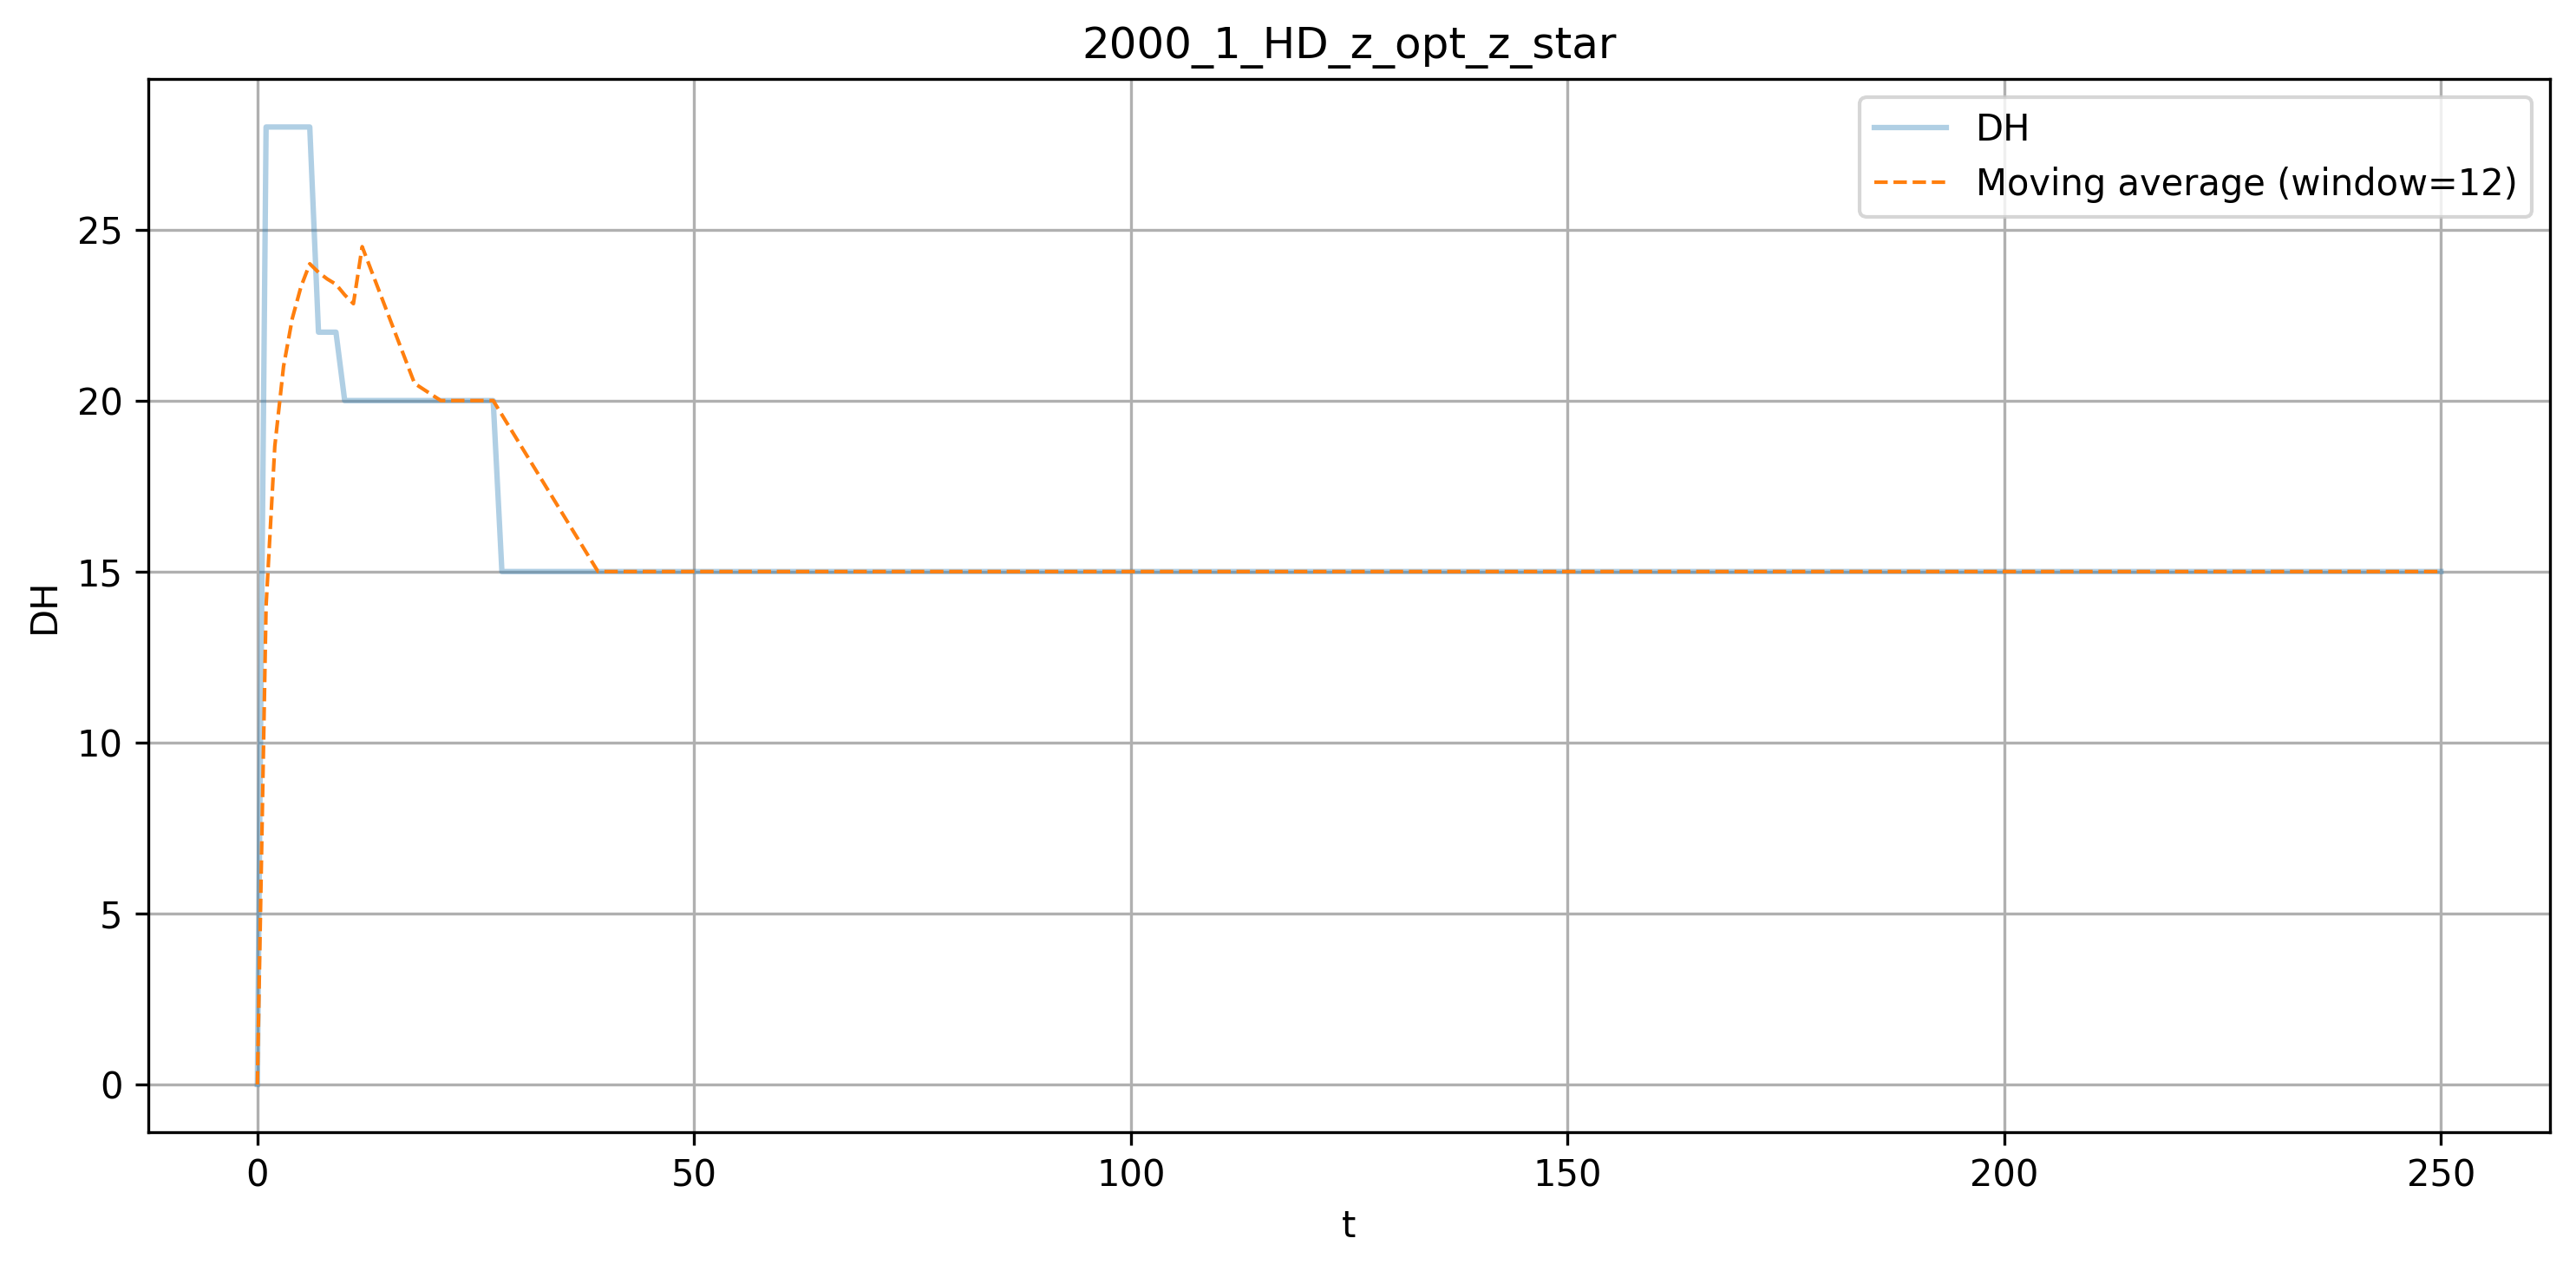
\includegraphics[width=\linewidth]{../Quantum-Annealing-for-solving-QUBO-Problems/test/Diagnostica_QALS/2/ksp_2/lambda_650_dot_C/2000_1_HD_z_opt_z_star.png}
    \caption{\(d_H(z_{opt}, z_\star)\) con \(\lambda_1\)}
    \label{fig:hd-zopt-zstar-lambda1}
\end{subfigure}
\hfill
\begin{subfigure}{0.495\textwidth}
    \centering
    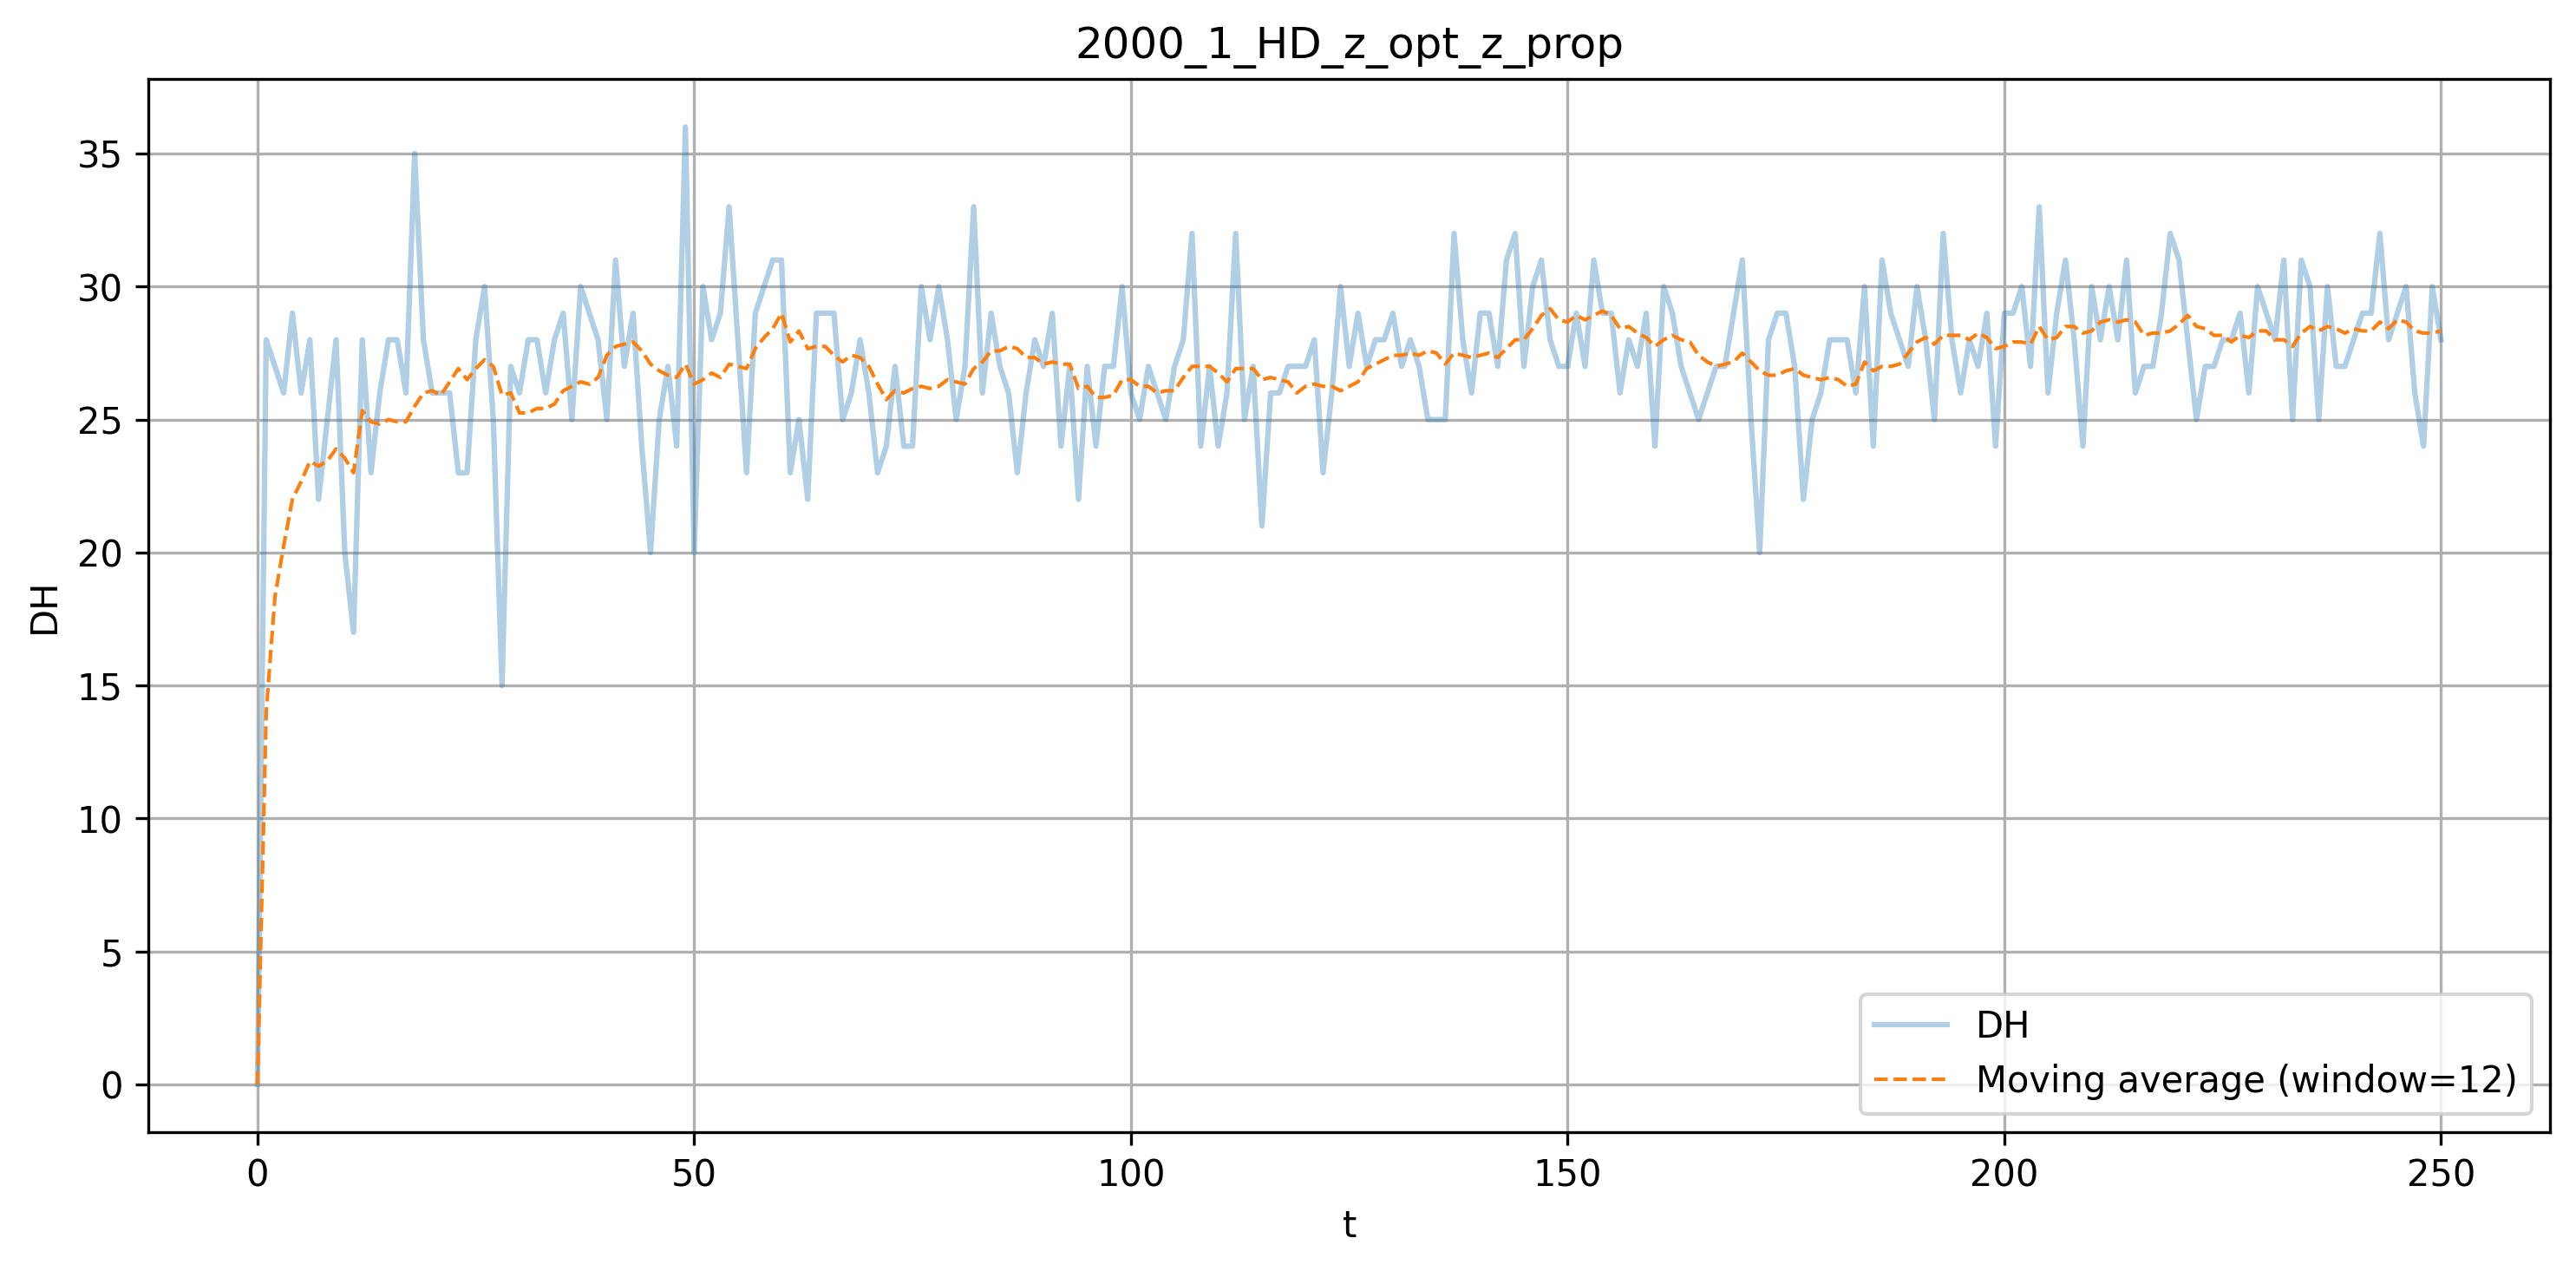
\includegraphics[width=\linewidth]{../Quantum-Annealing-for-solving-QUBO-Problems/test/Diagnostica_QALS/2/ksp_2/lambda_650_dot_C/2000_1_HD_z_opt_z_prop.png}
    \caption{\(d_H(z_{opt}, z_t)\) con \(\lambda_1\)}
    \label{fig:hd-zopt-zt-lambda1}
\end{subfigure}

\vspace{0.35cm}

\begin{subfigure}{0.495\textwidth}
    \centering
    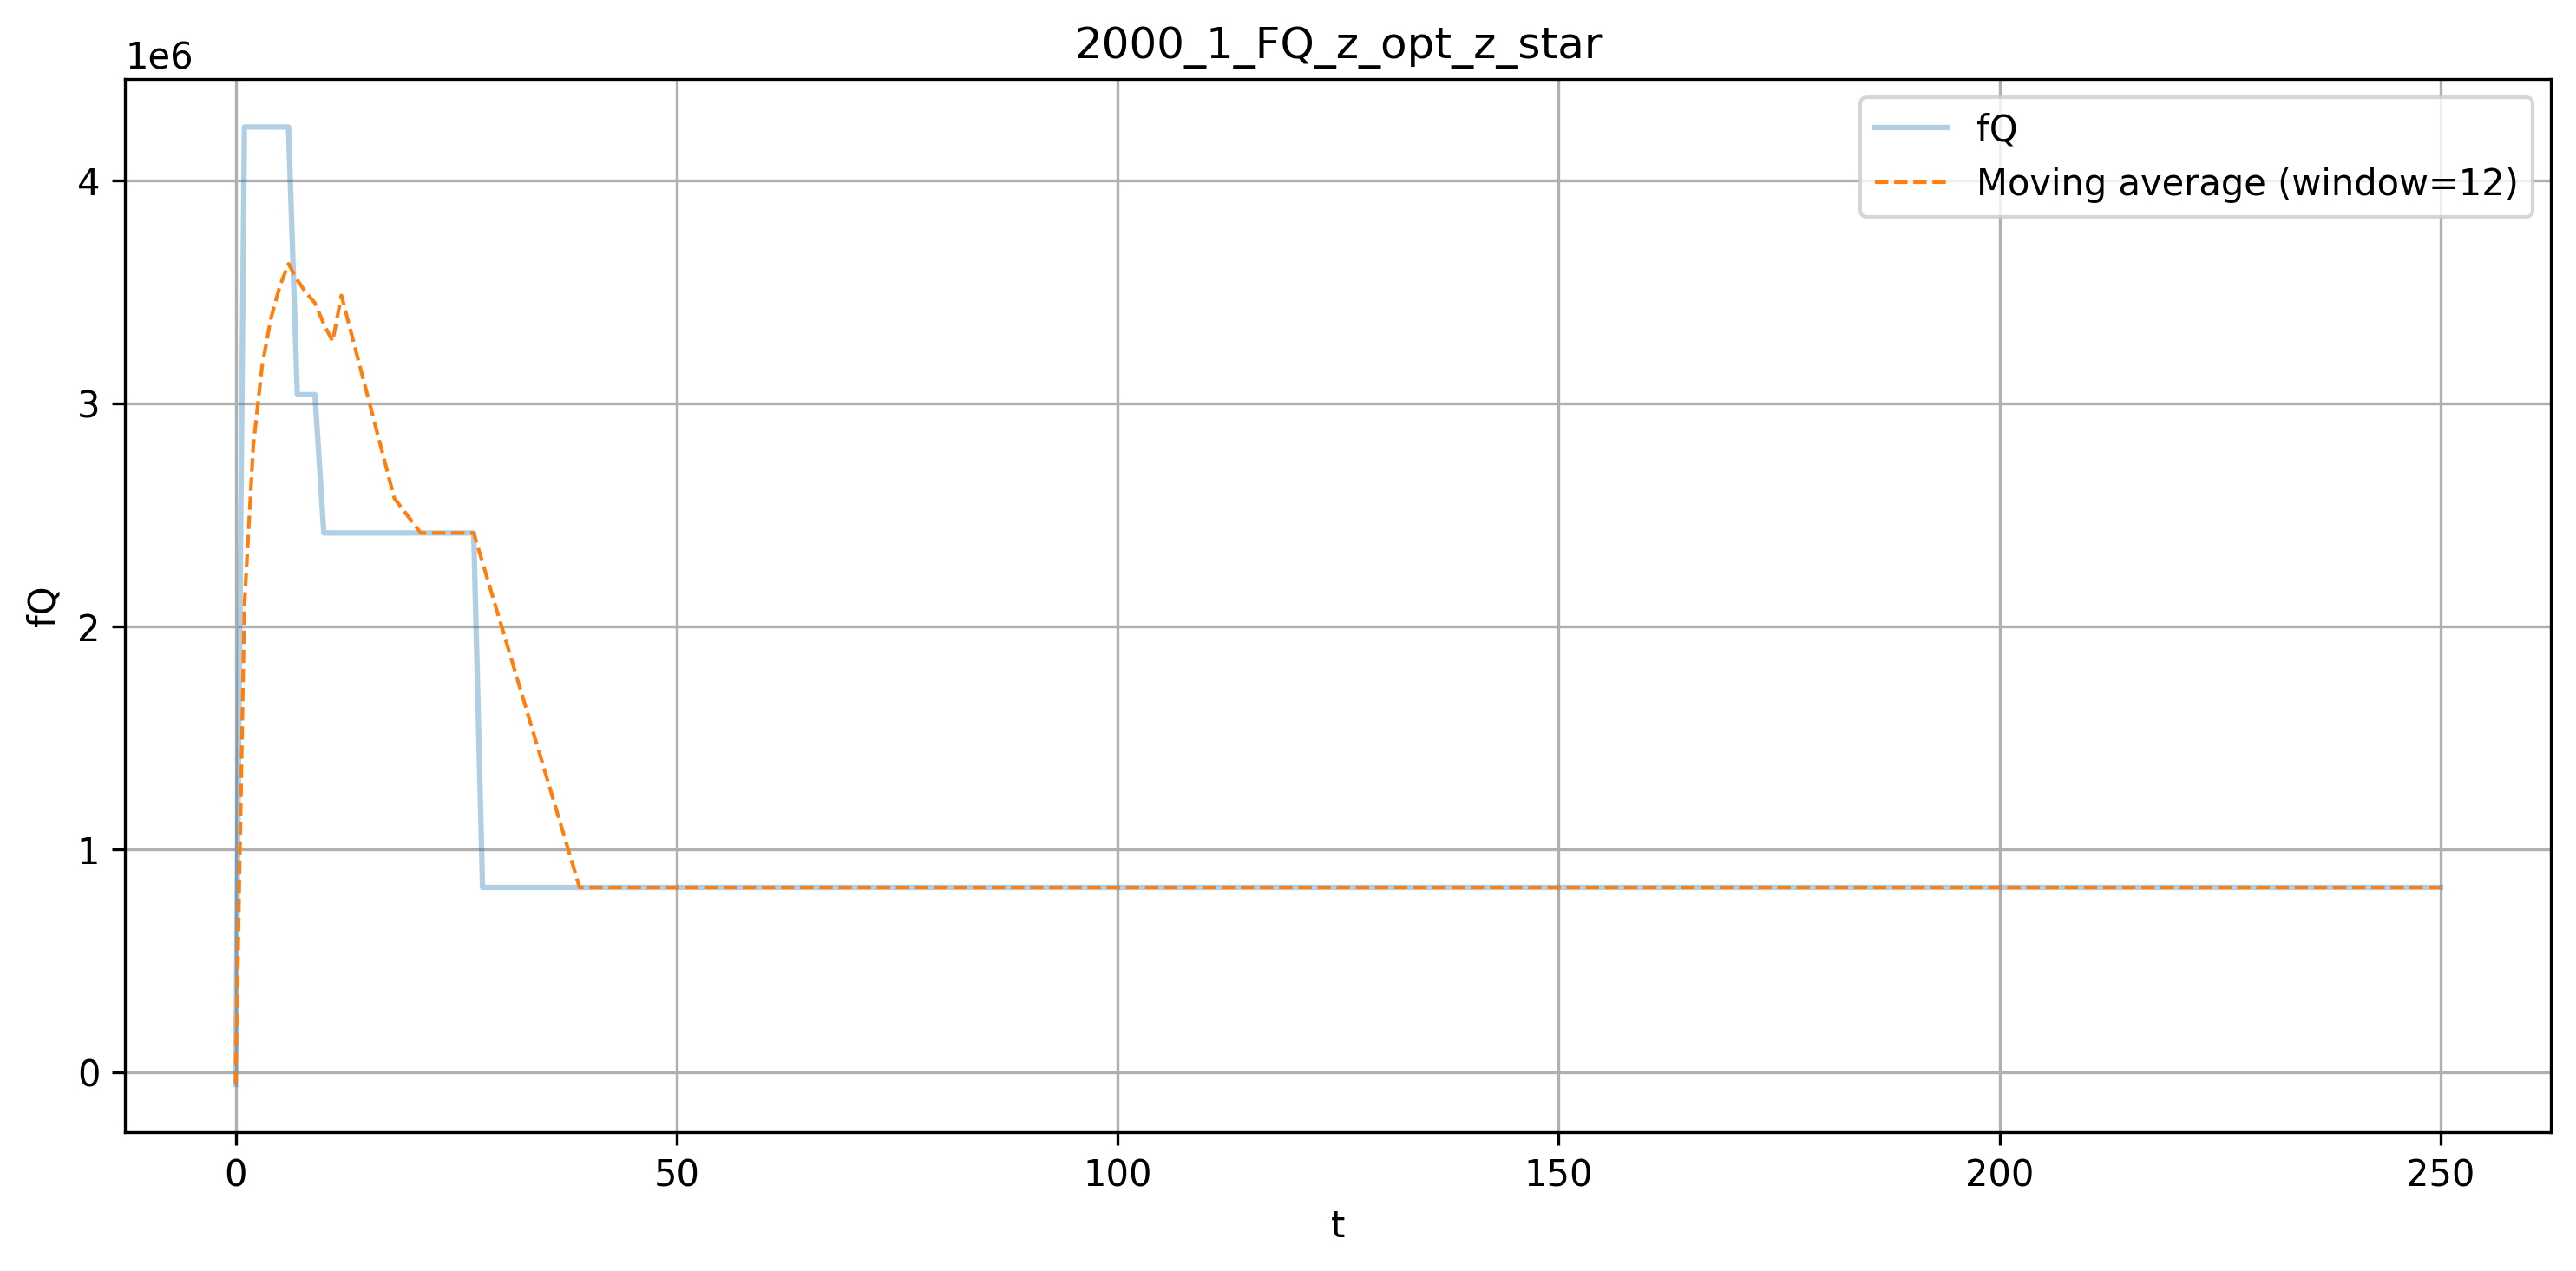
\includegraphics[width=\linewidth]{../Quantum-Annealing-for-solving-QUBO-Problems/test/Diagnostica_QALS/2/ksp_2/lambda_650_dot_C/2000_1_FQ_z_opt_z_star.png}
    \caption{\(f_Q(z_\star)\) con \(\lambda_1\)}
    \label{fig:fQ-zstar-lambda1}
\end{subfigure}
\hfill
\begin{subfigure}{0.495\textwidth}
    \centering
    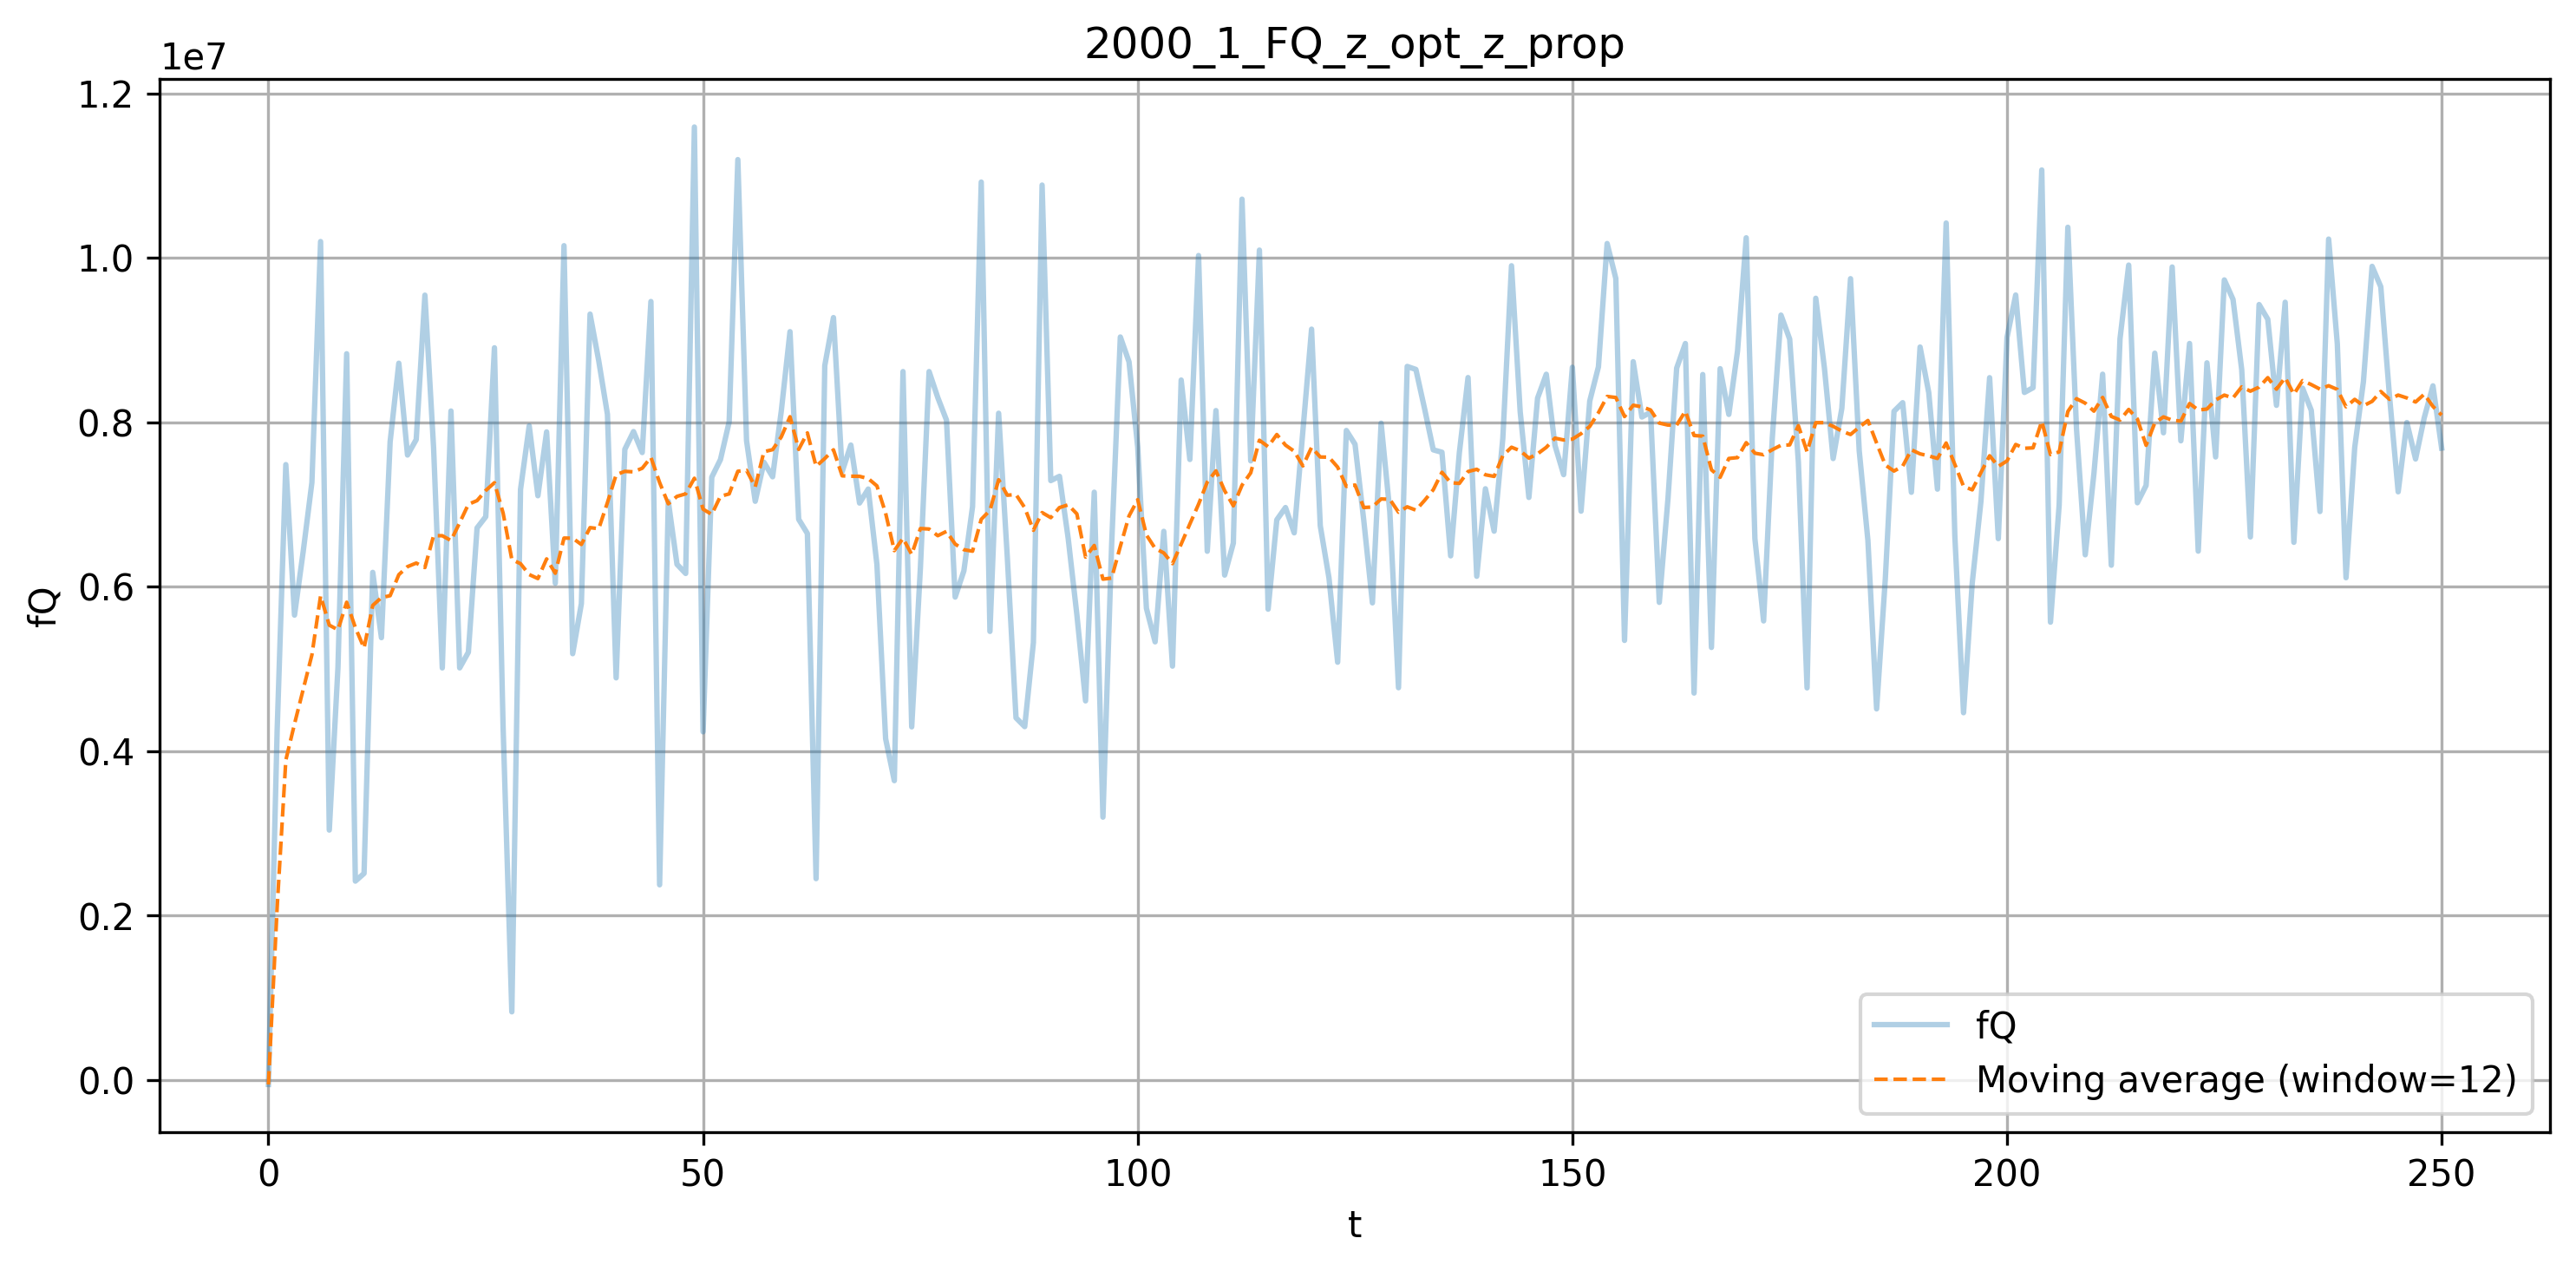
\includegraphics[width=\linewidth]{../Quantum-Annealing-for-solving-QUBO-Problems/test/Diagnostica_QALS/2/ksp_2/lambda_650_dot_C/2000_1_FQ_z_opt_z_prop.png}
    \caption{\(f_Q(z_t)\) con \(\lambda_1\)}
    \label{fig:fQ-zt-lambda1}
\end{subfigure}
\label{fig:confronto-hamming-ksp21}
\end{figure}

\begin{figure}[H]
\centering
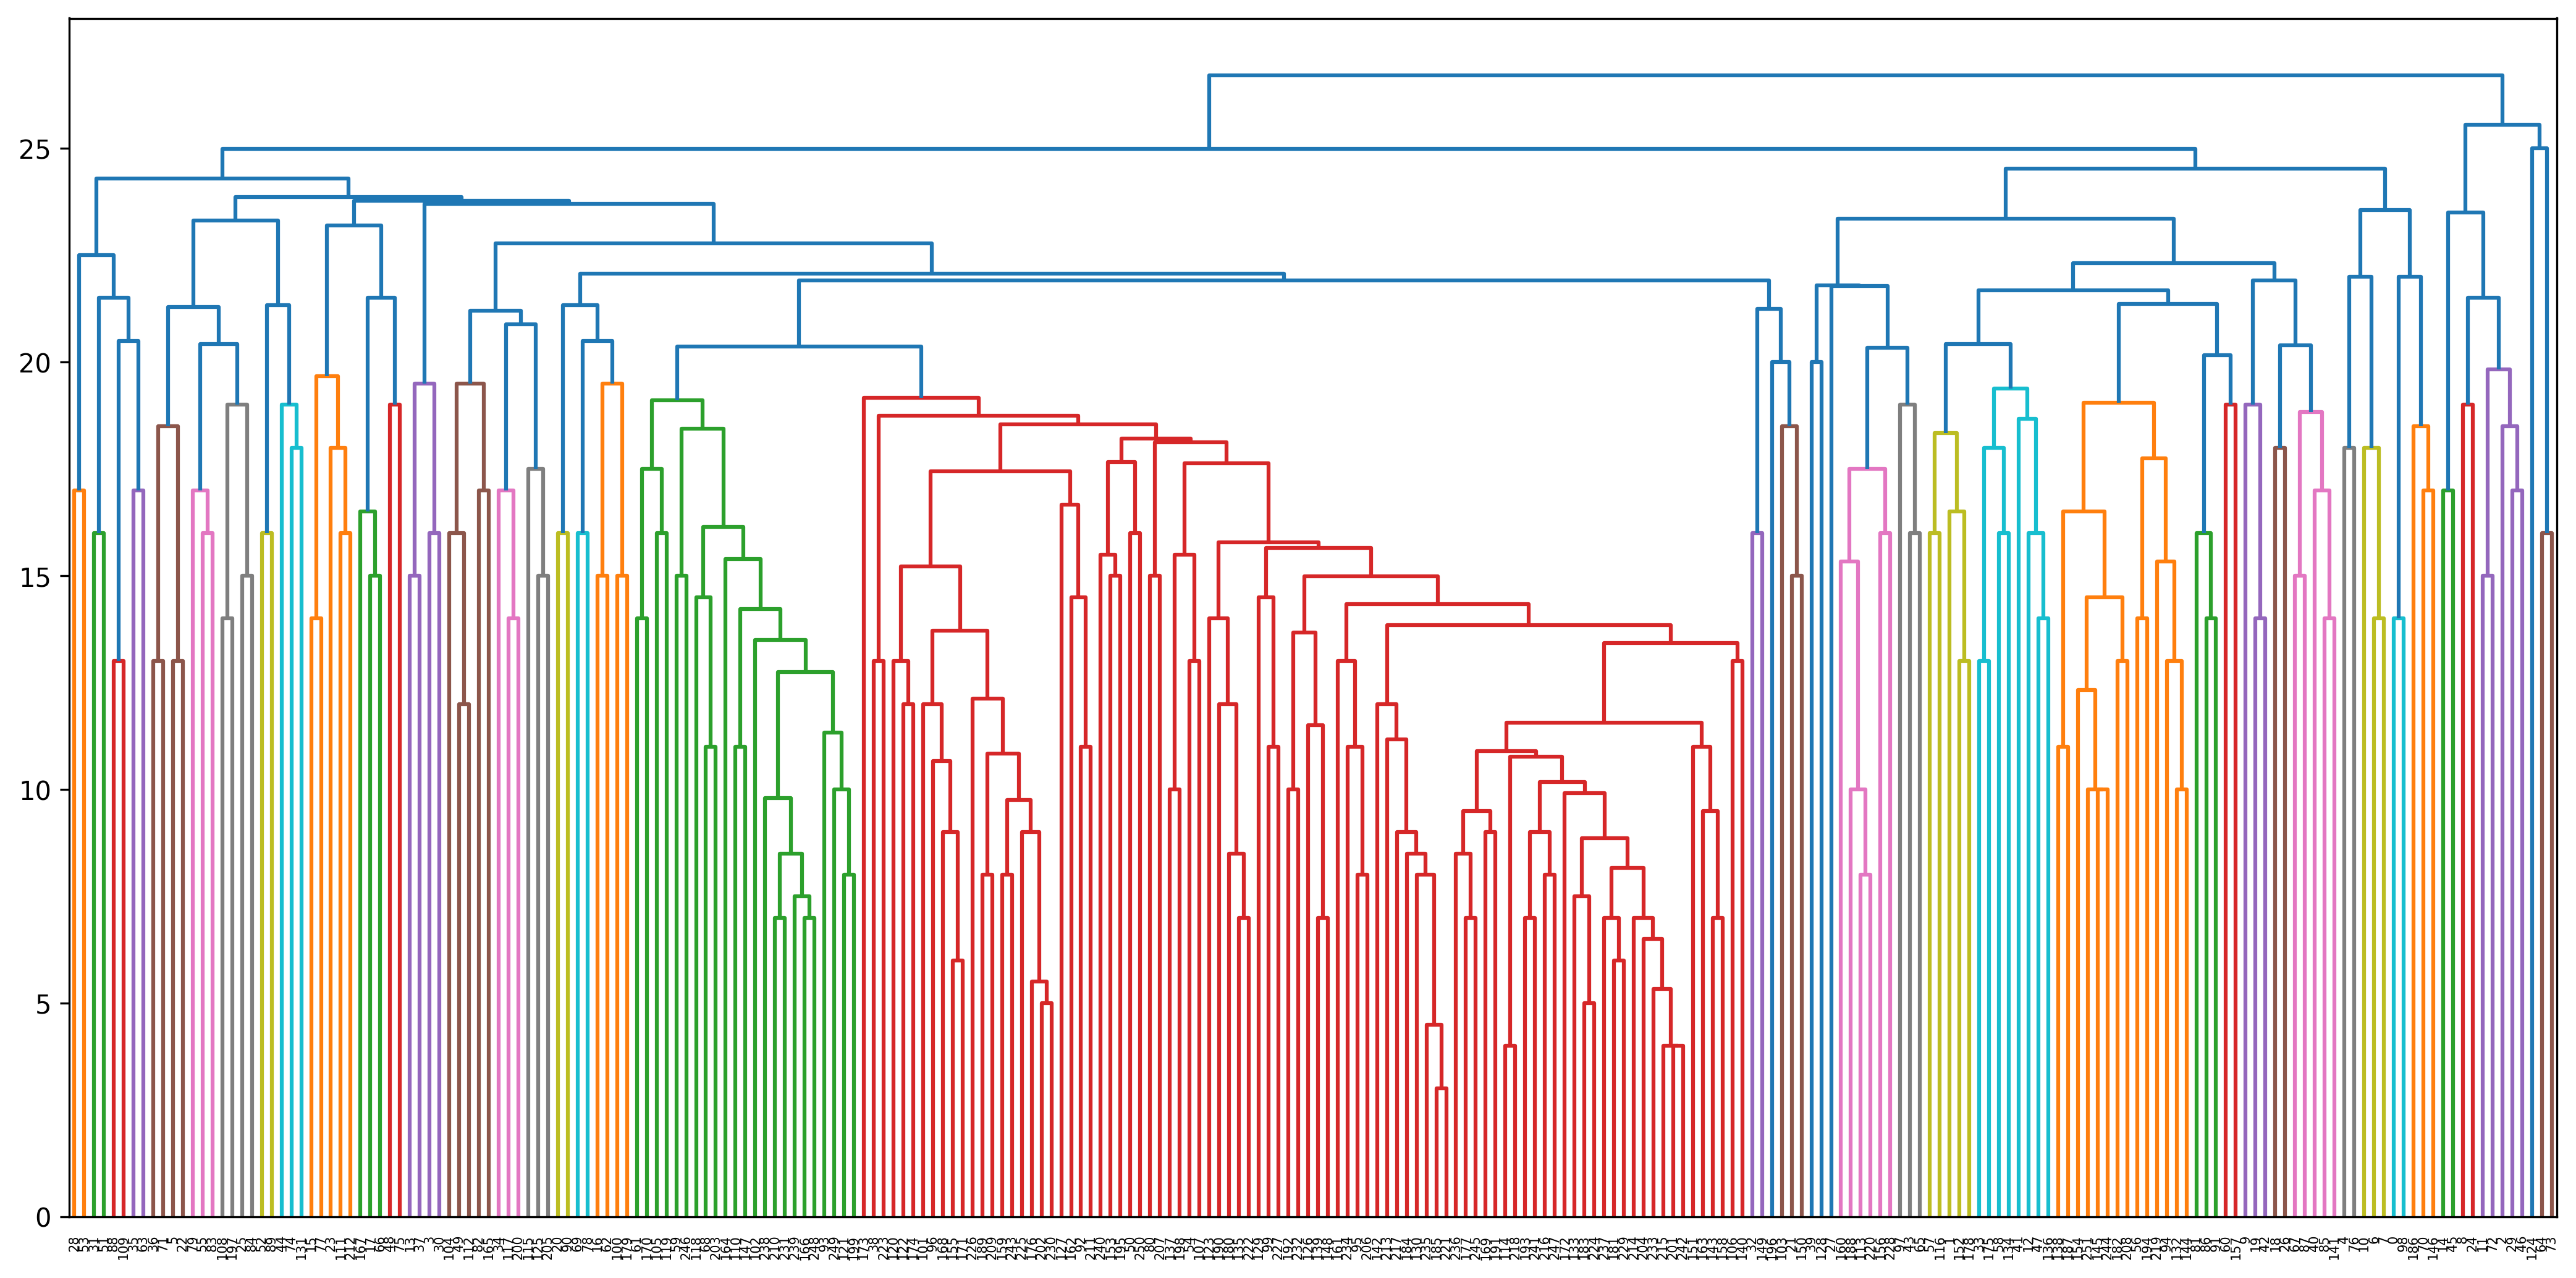
\includegraphics[width=\linewidth]{../Quantum-Annealing-for-solving-QUBO-Problems/test/Diagnostica_QALS/2/ksp_2/lambda_650_dot_C/dendrogram_2000_1.png}
\caption{Agglomerative Clustering Dendogram}
\label{fig:AgglomerativeClustering-ksp2}
\end{figure}

\clearpage
\begin{figure}[H]
\centering
\begin{subfigure}{0.495\textwidth}
    \centering
    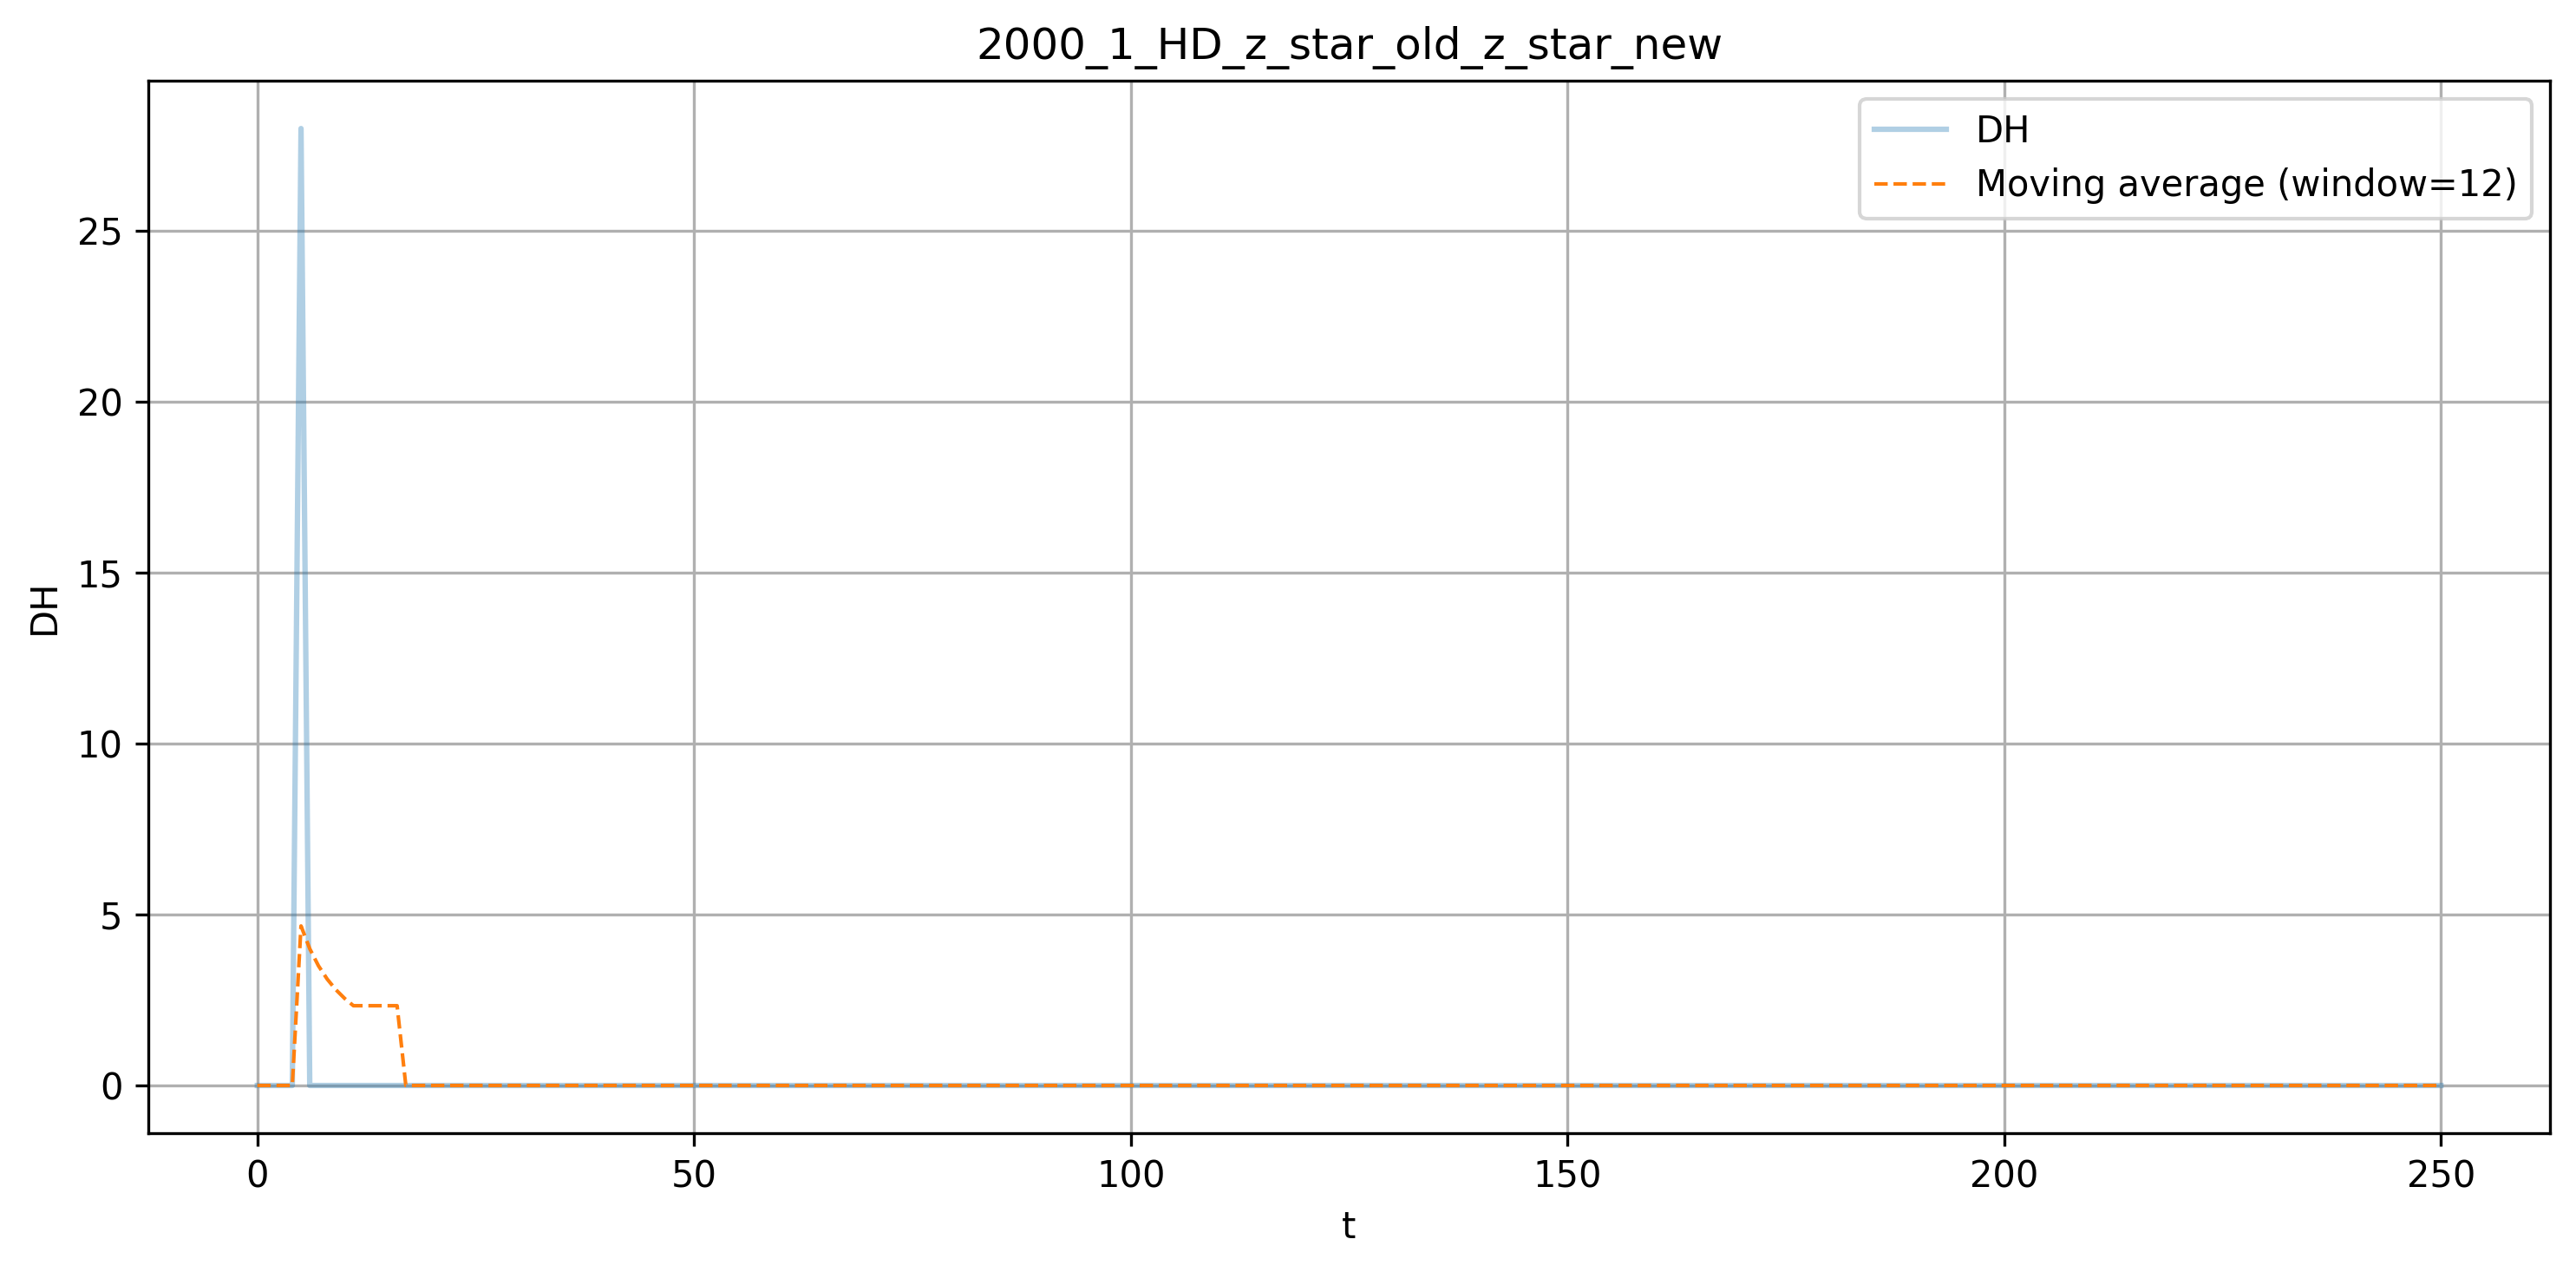
\includegraphics[width=\linewidth]{../Quantum-Annealing-for-solving-QUBO-Problems/test/Diagnostica_QALS/2/ksp_2/lambda_div_3/2000_1_HD_z_star_old_z_star_new.png}
    \caption{\(d_H(z_\star^{old}, z_\star^{new})\) con \(\lambda_2\)}
    \label{fig:hd-zstarold-zstarnew-lambda2}
\end{subfigure}
\hfill
\begin{subfigure}{0.495\textwidth}
    \centering
    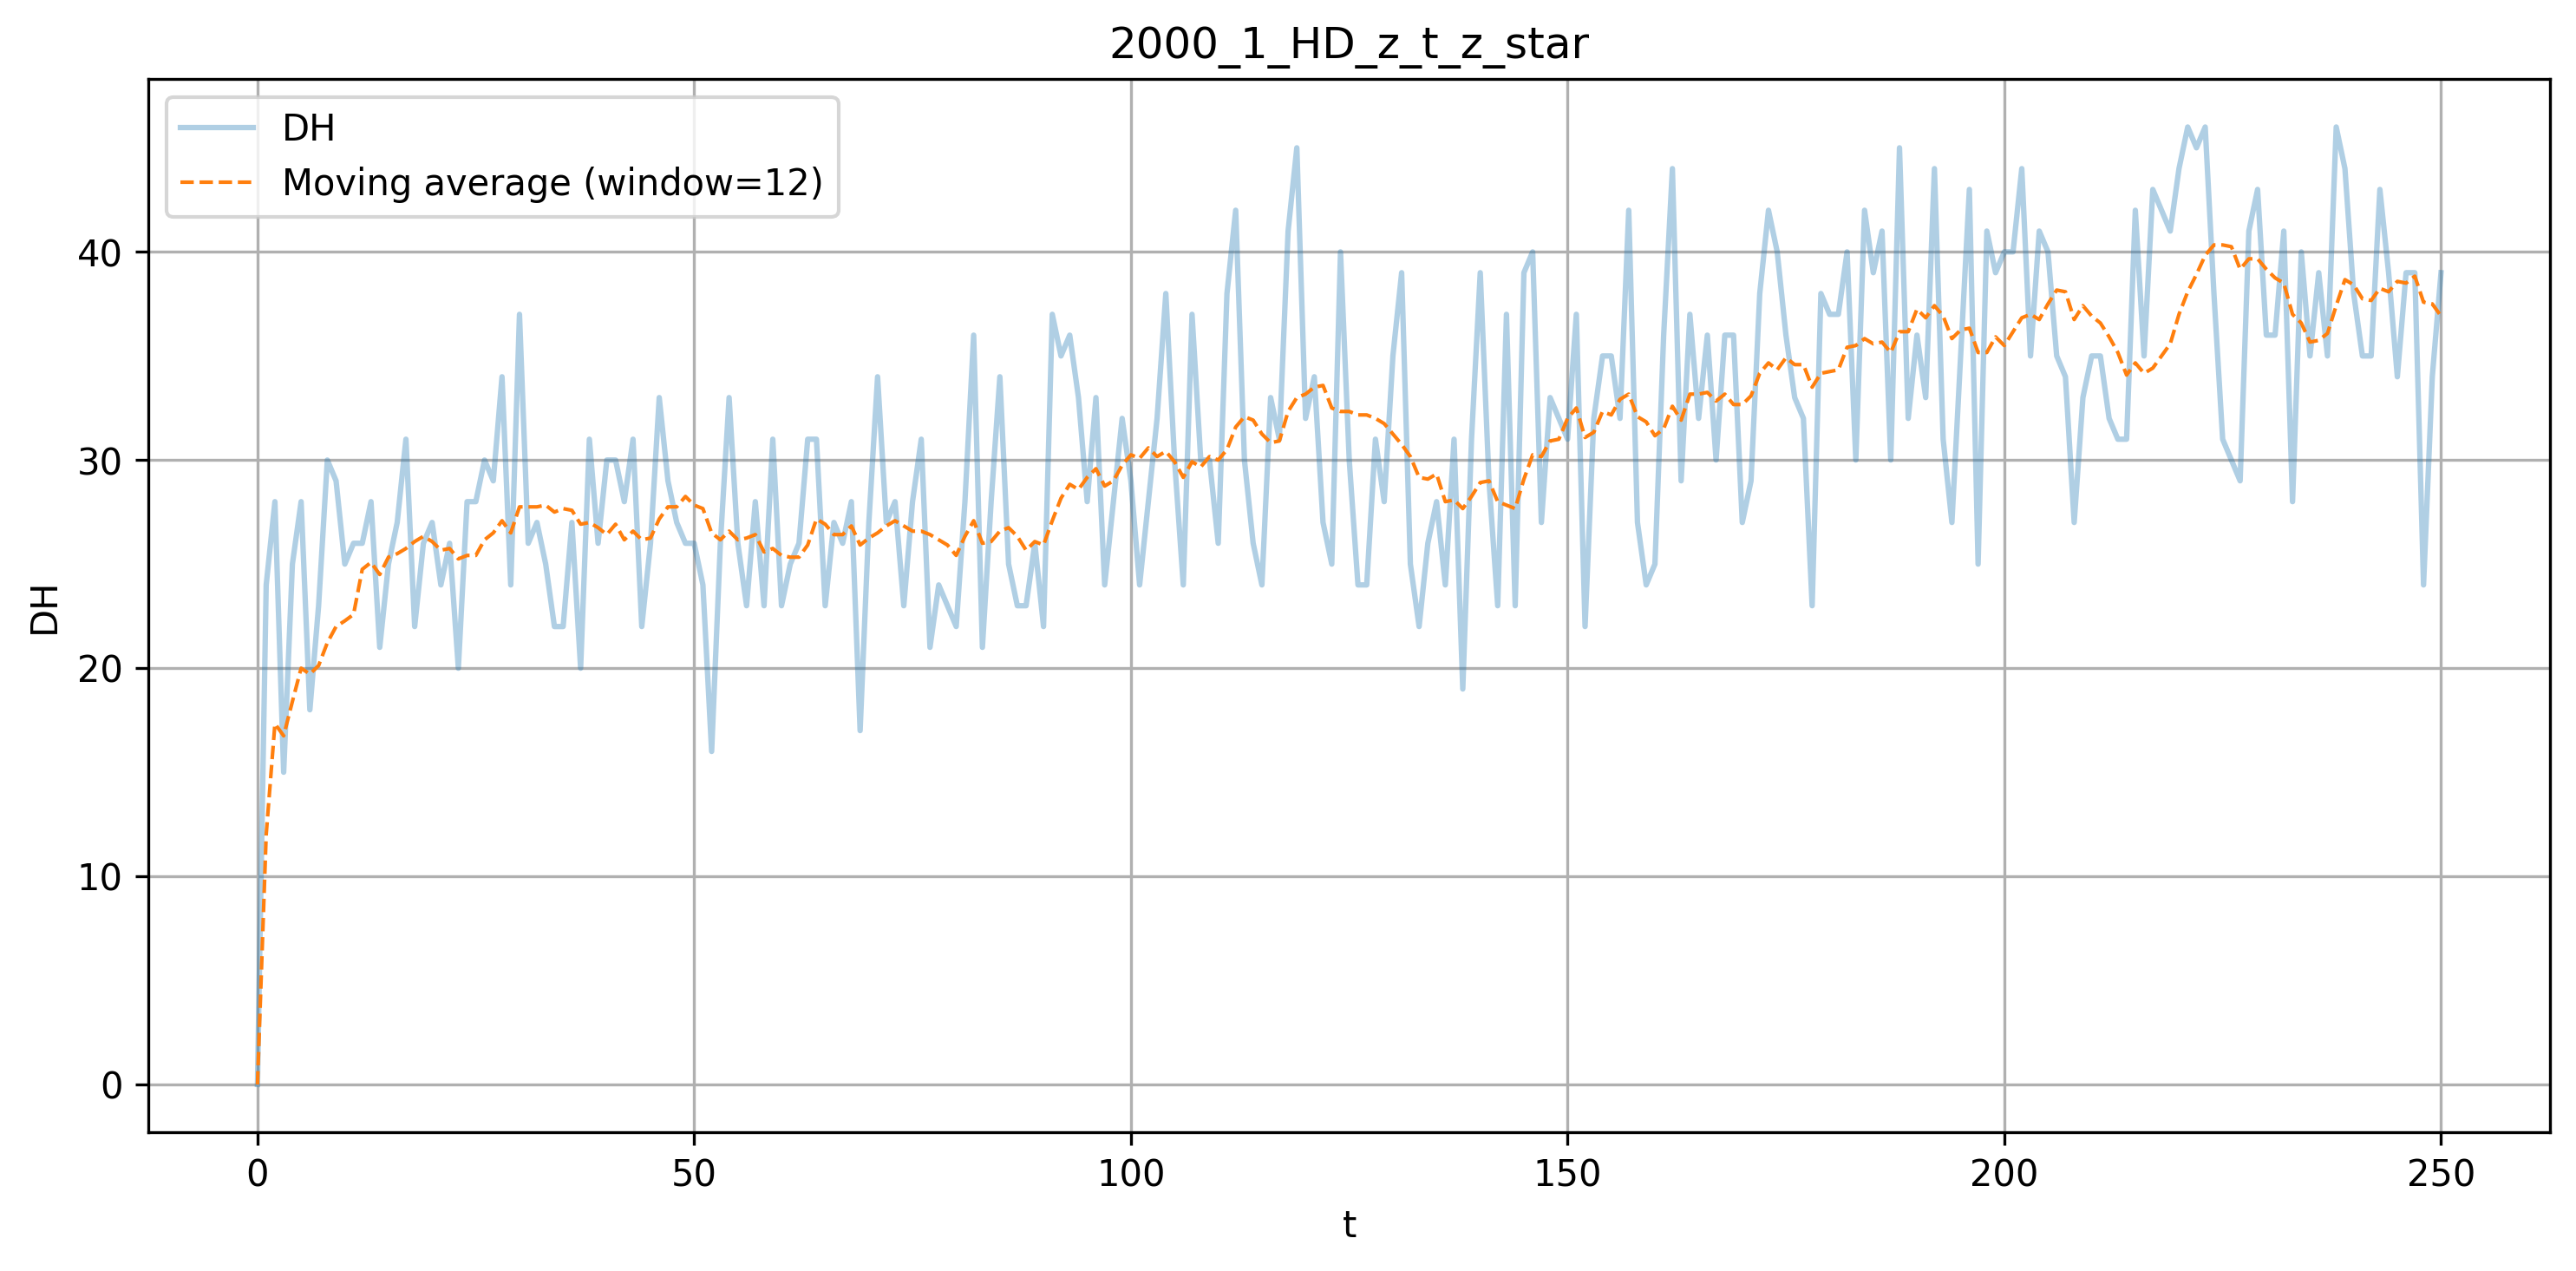
\includegraphics[width=\linewidth]{../Quantum-Annealing-for-solving-QUBO-Problems/test/Diagnostica_QALS/2/ksp_2/lambda_div_3/2000_1_HD_z_t_z_star.png}
    \caption{\(d_H(z_t, z_\star)\) con \(\lambda_2\)}
    \label{fig:hd-zt-zstar-lambda2}
\end{subfigure}

\vspace{0.35cm}

\begin{subfigure}{0.495\textwidth}
    \centering
    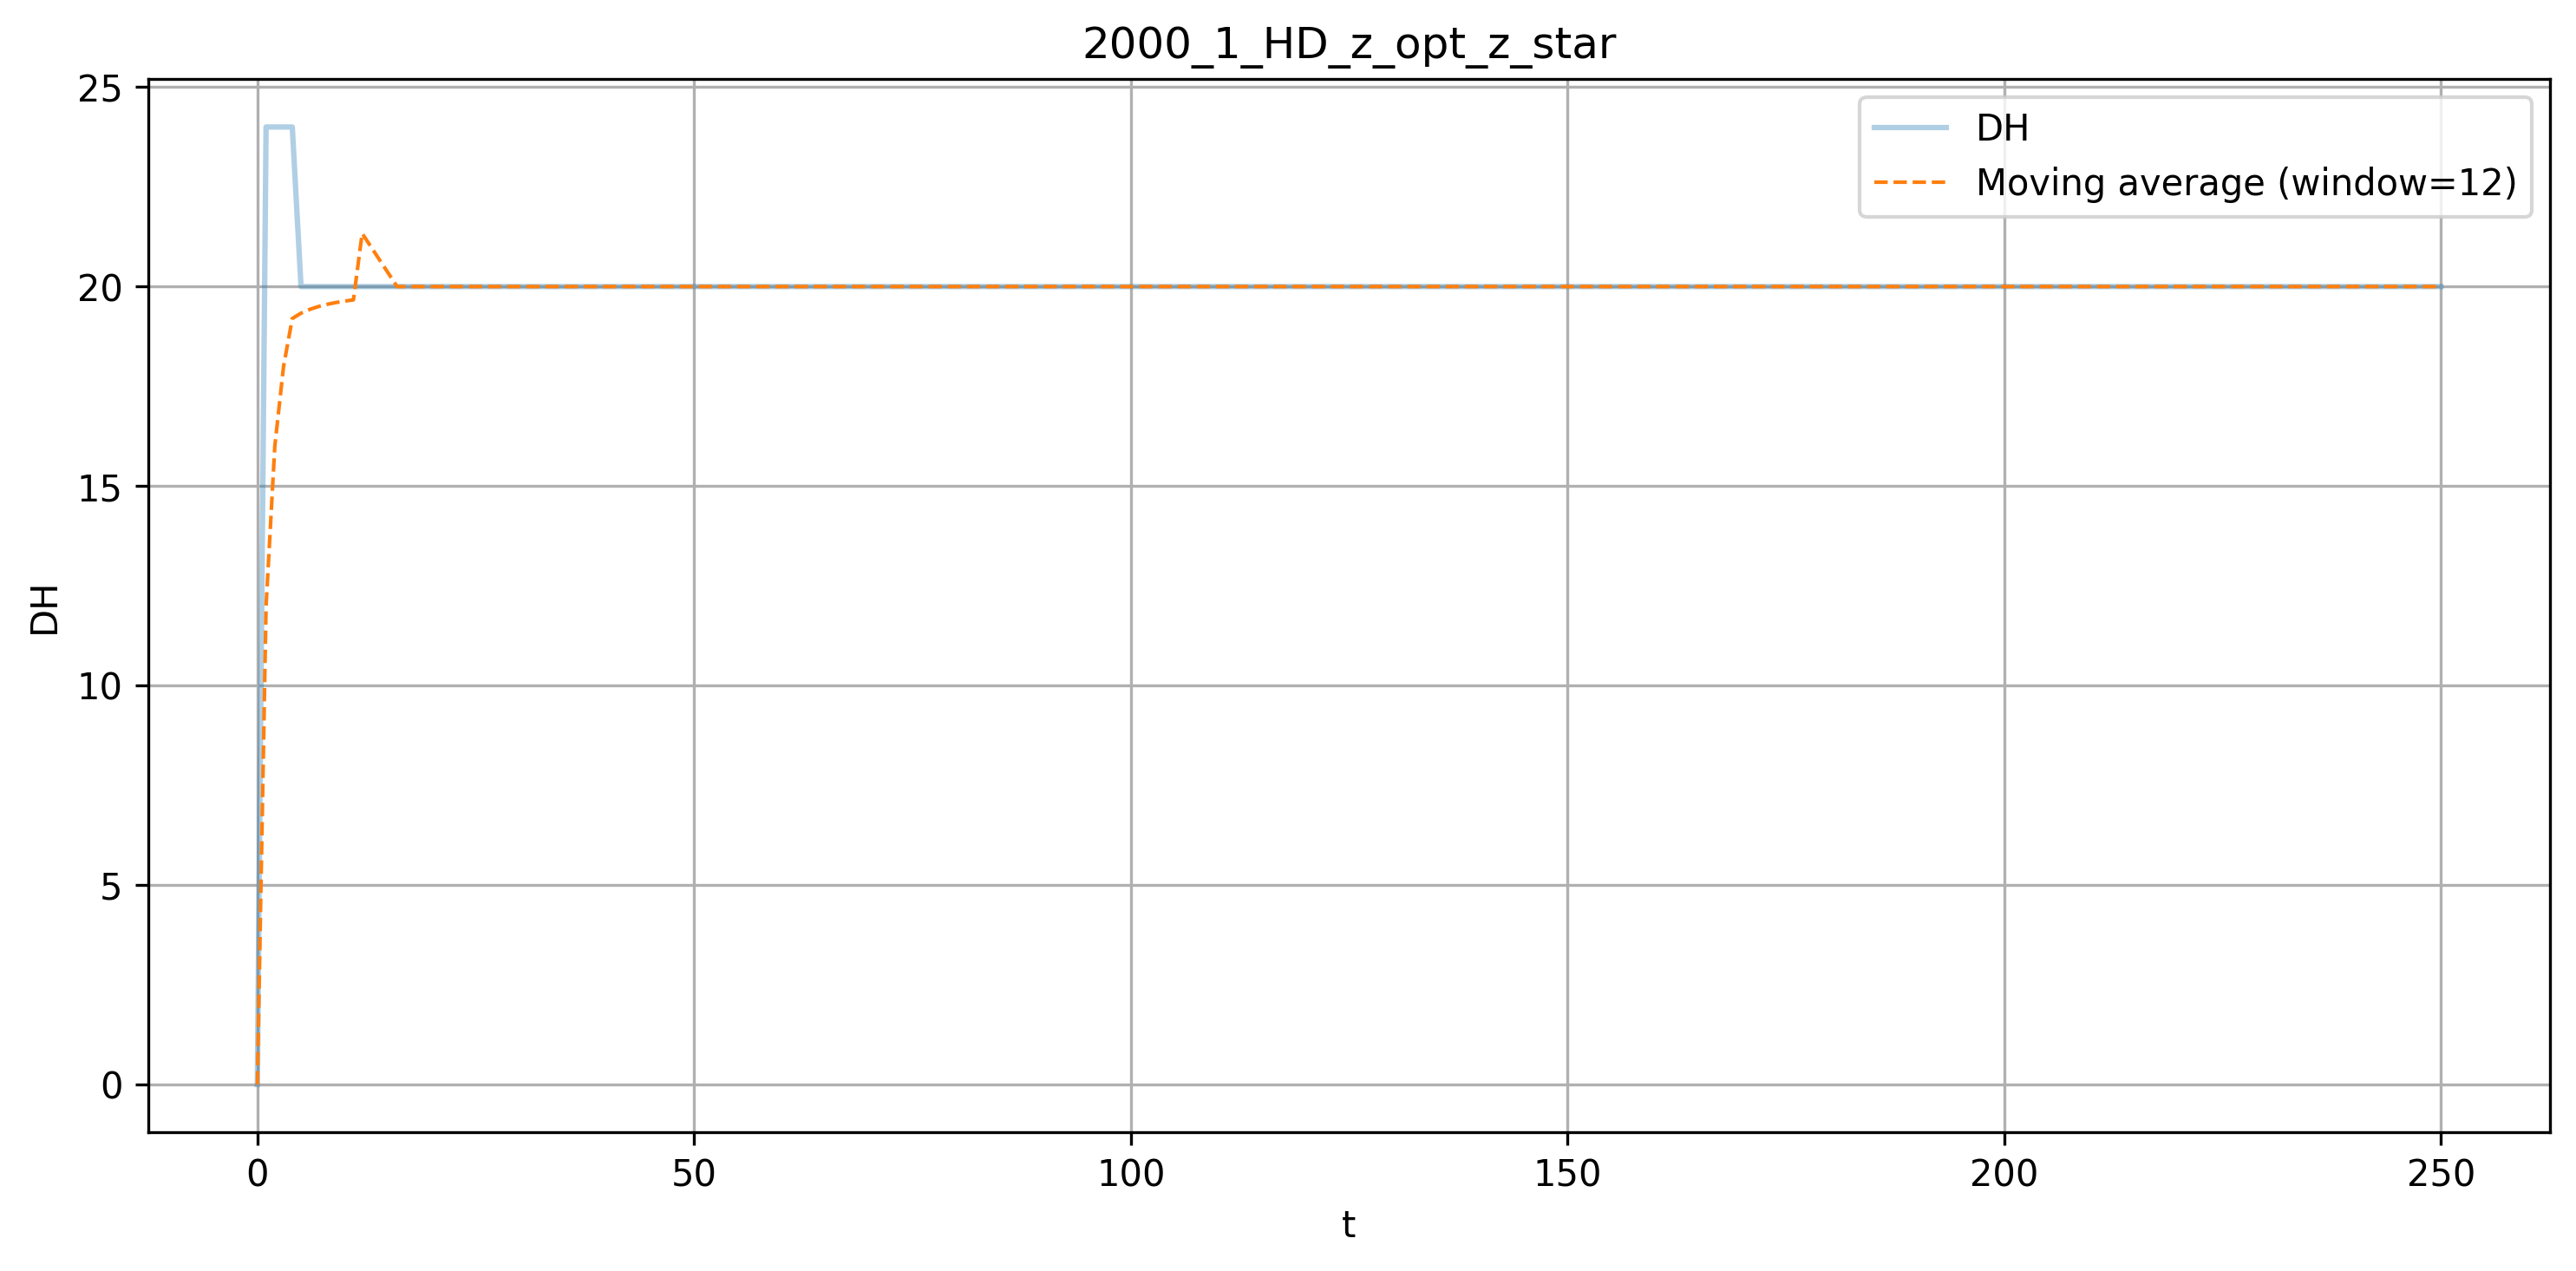
\includegraphics[width=\linewidth]{../Quantum-Annealing-for-solving-QUBO-Problems/test/Diagnostica_QALS/2/ksp_2/lambda_div_3/2000_1_HD_z_opt_z_star.png}
    \caption{\(d_H(z_{opt}, z_\star)\) con \(\lambda_2\)}
    \label{fig:hd-zopt-zstar-lambda2}
\end{subfigure}
\hfill
\begin{subfigure}{0.495\textwidth}
    \centering
    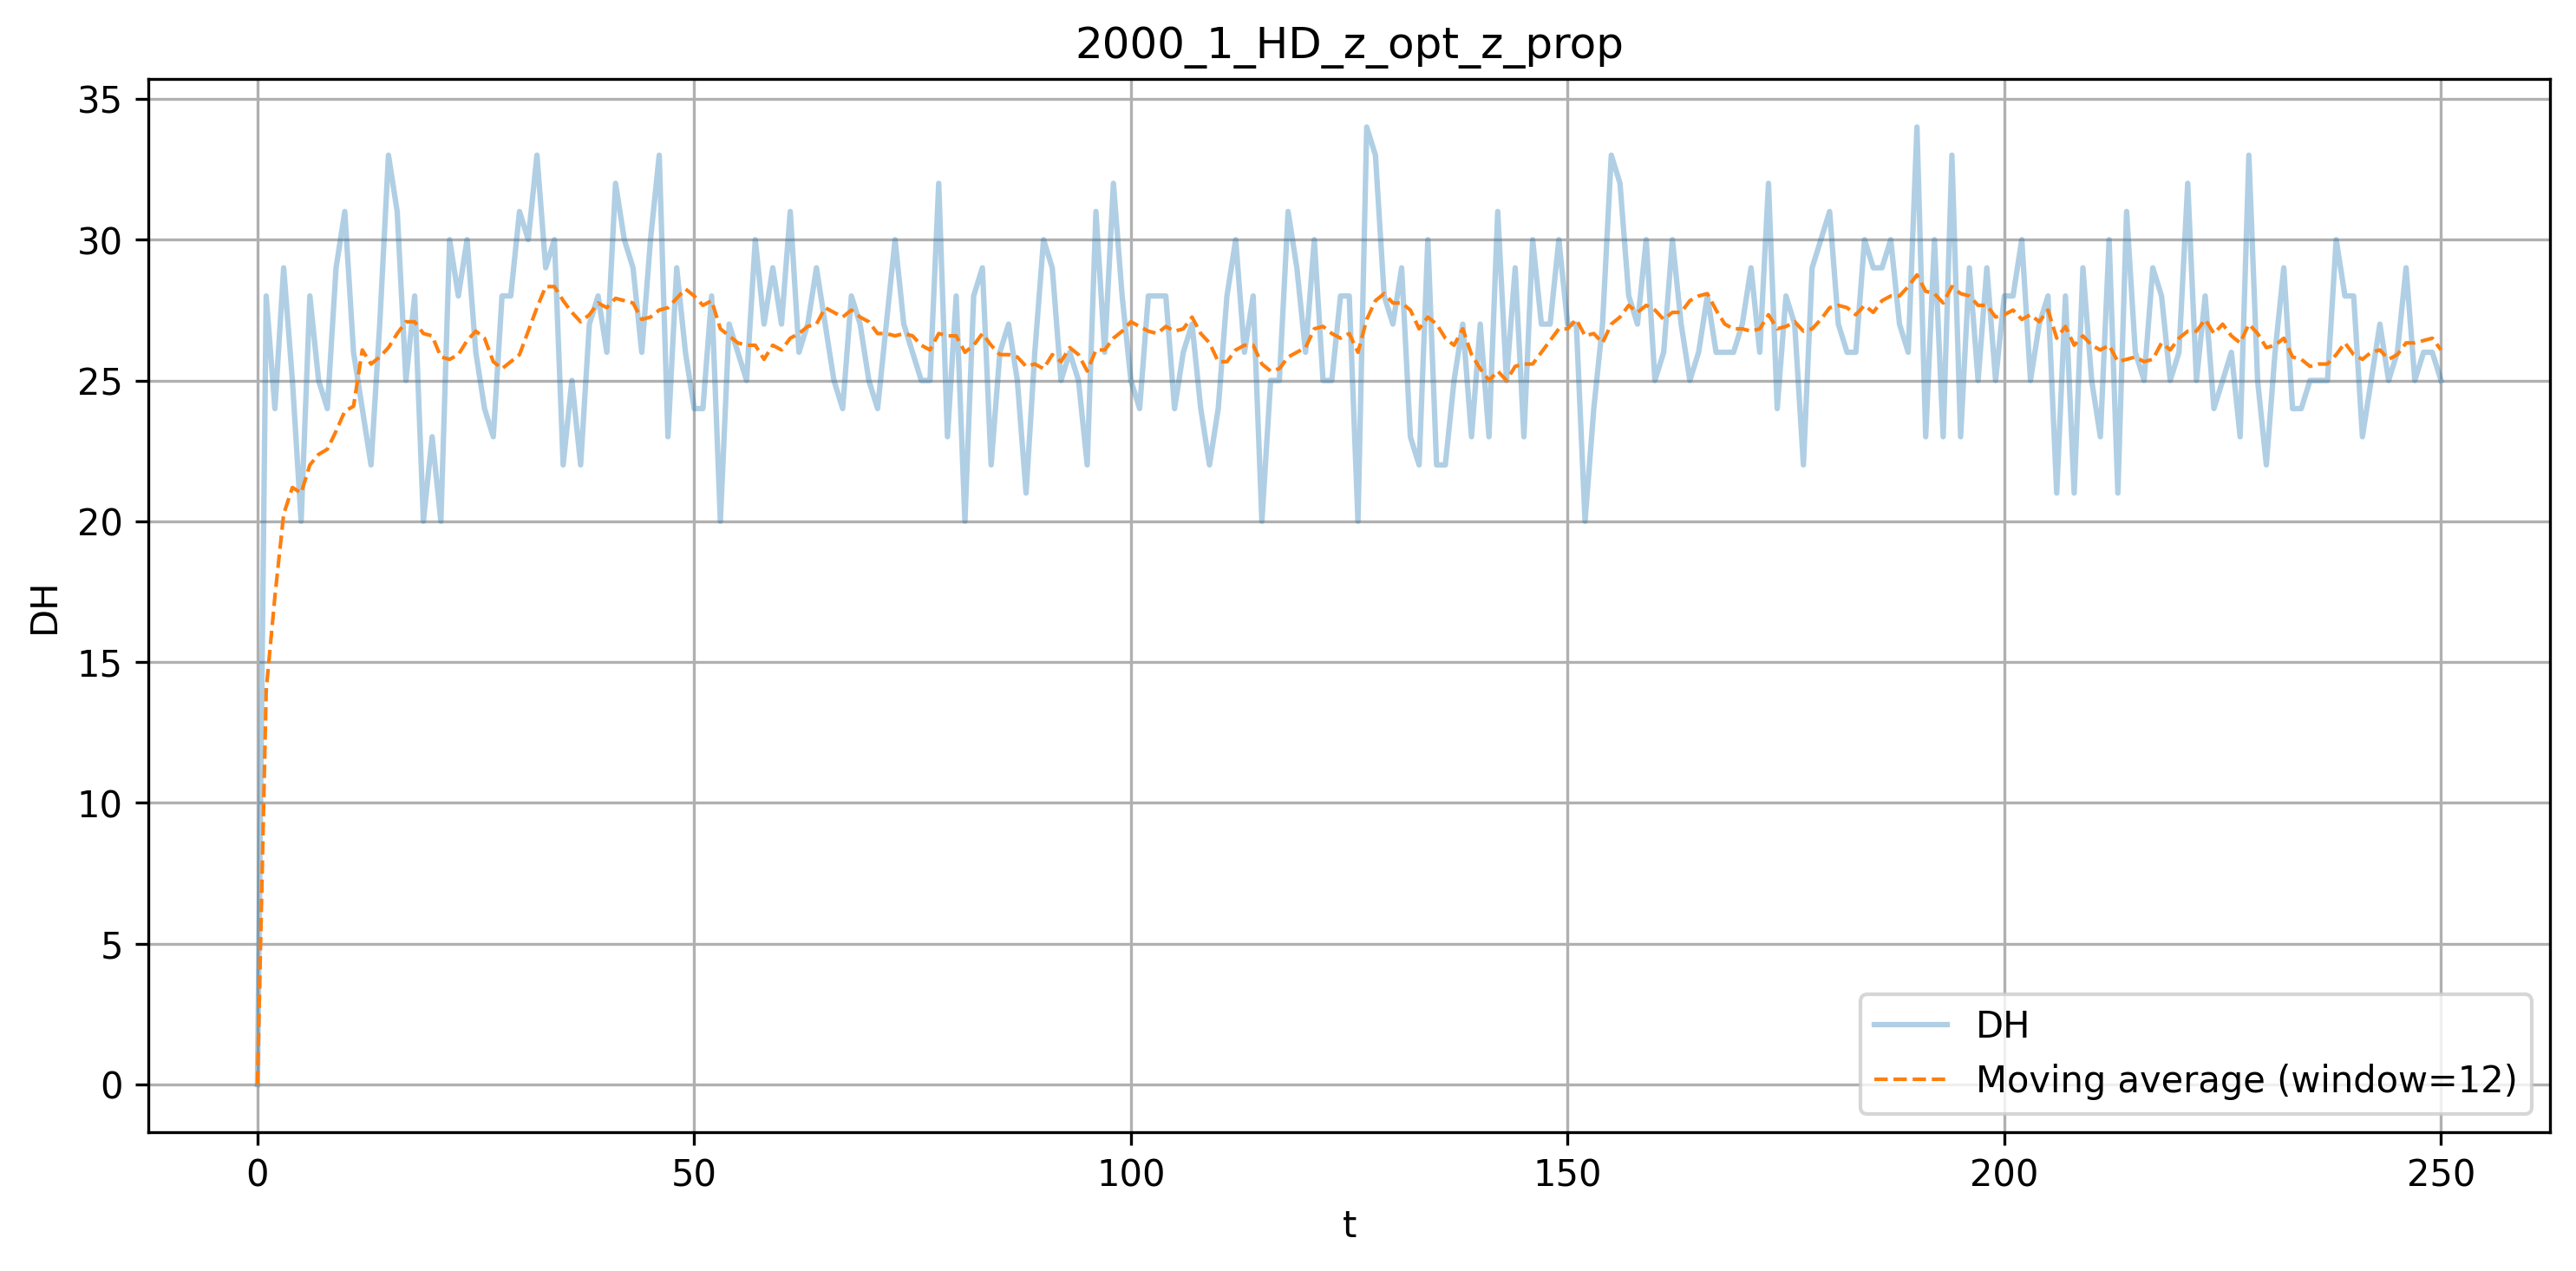
\includegraphics[width=\linewidth]{../Quantum-Annealing-for-solving-QUBO-Problems/test/Diagnostica_QALS/2/ksp_2/lambda_div_3/2000_1_HD_z_opt_z_prop.png}
    \caption{\(d_H(z_{opt}, z_t)\) con \(\lambda_2\)}
    \label{fig:hd-zopt-zt-lambda2}
\end{subfigure}

\vspace{0.35cm}

\begin{subfigure}{0.495\textwidth}
    \centering
    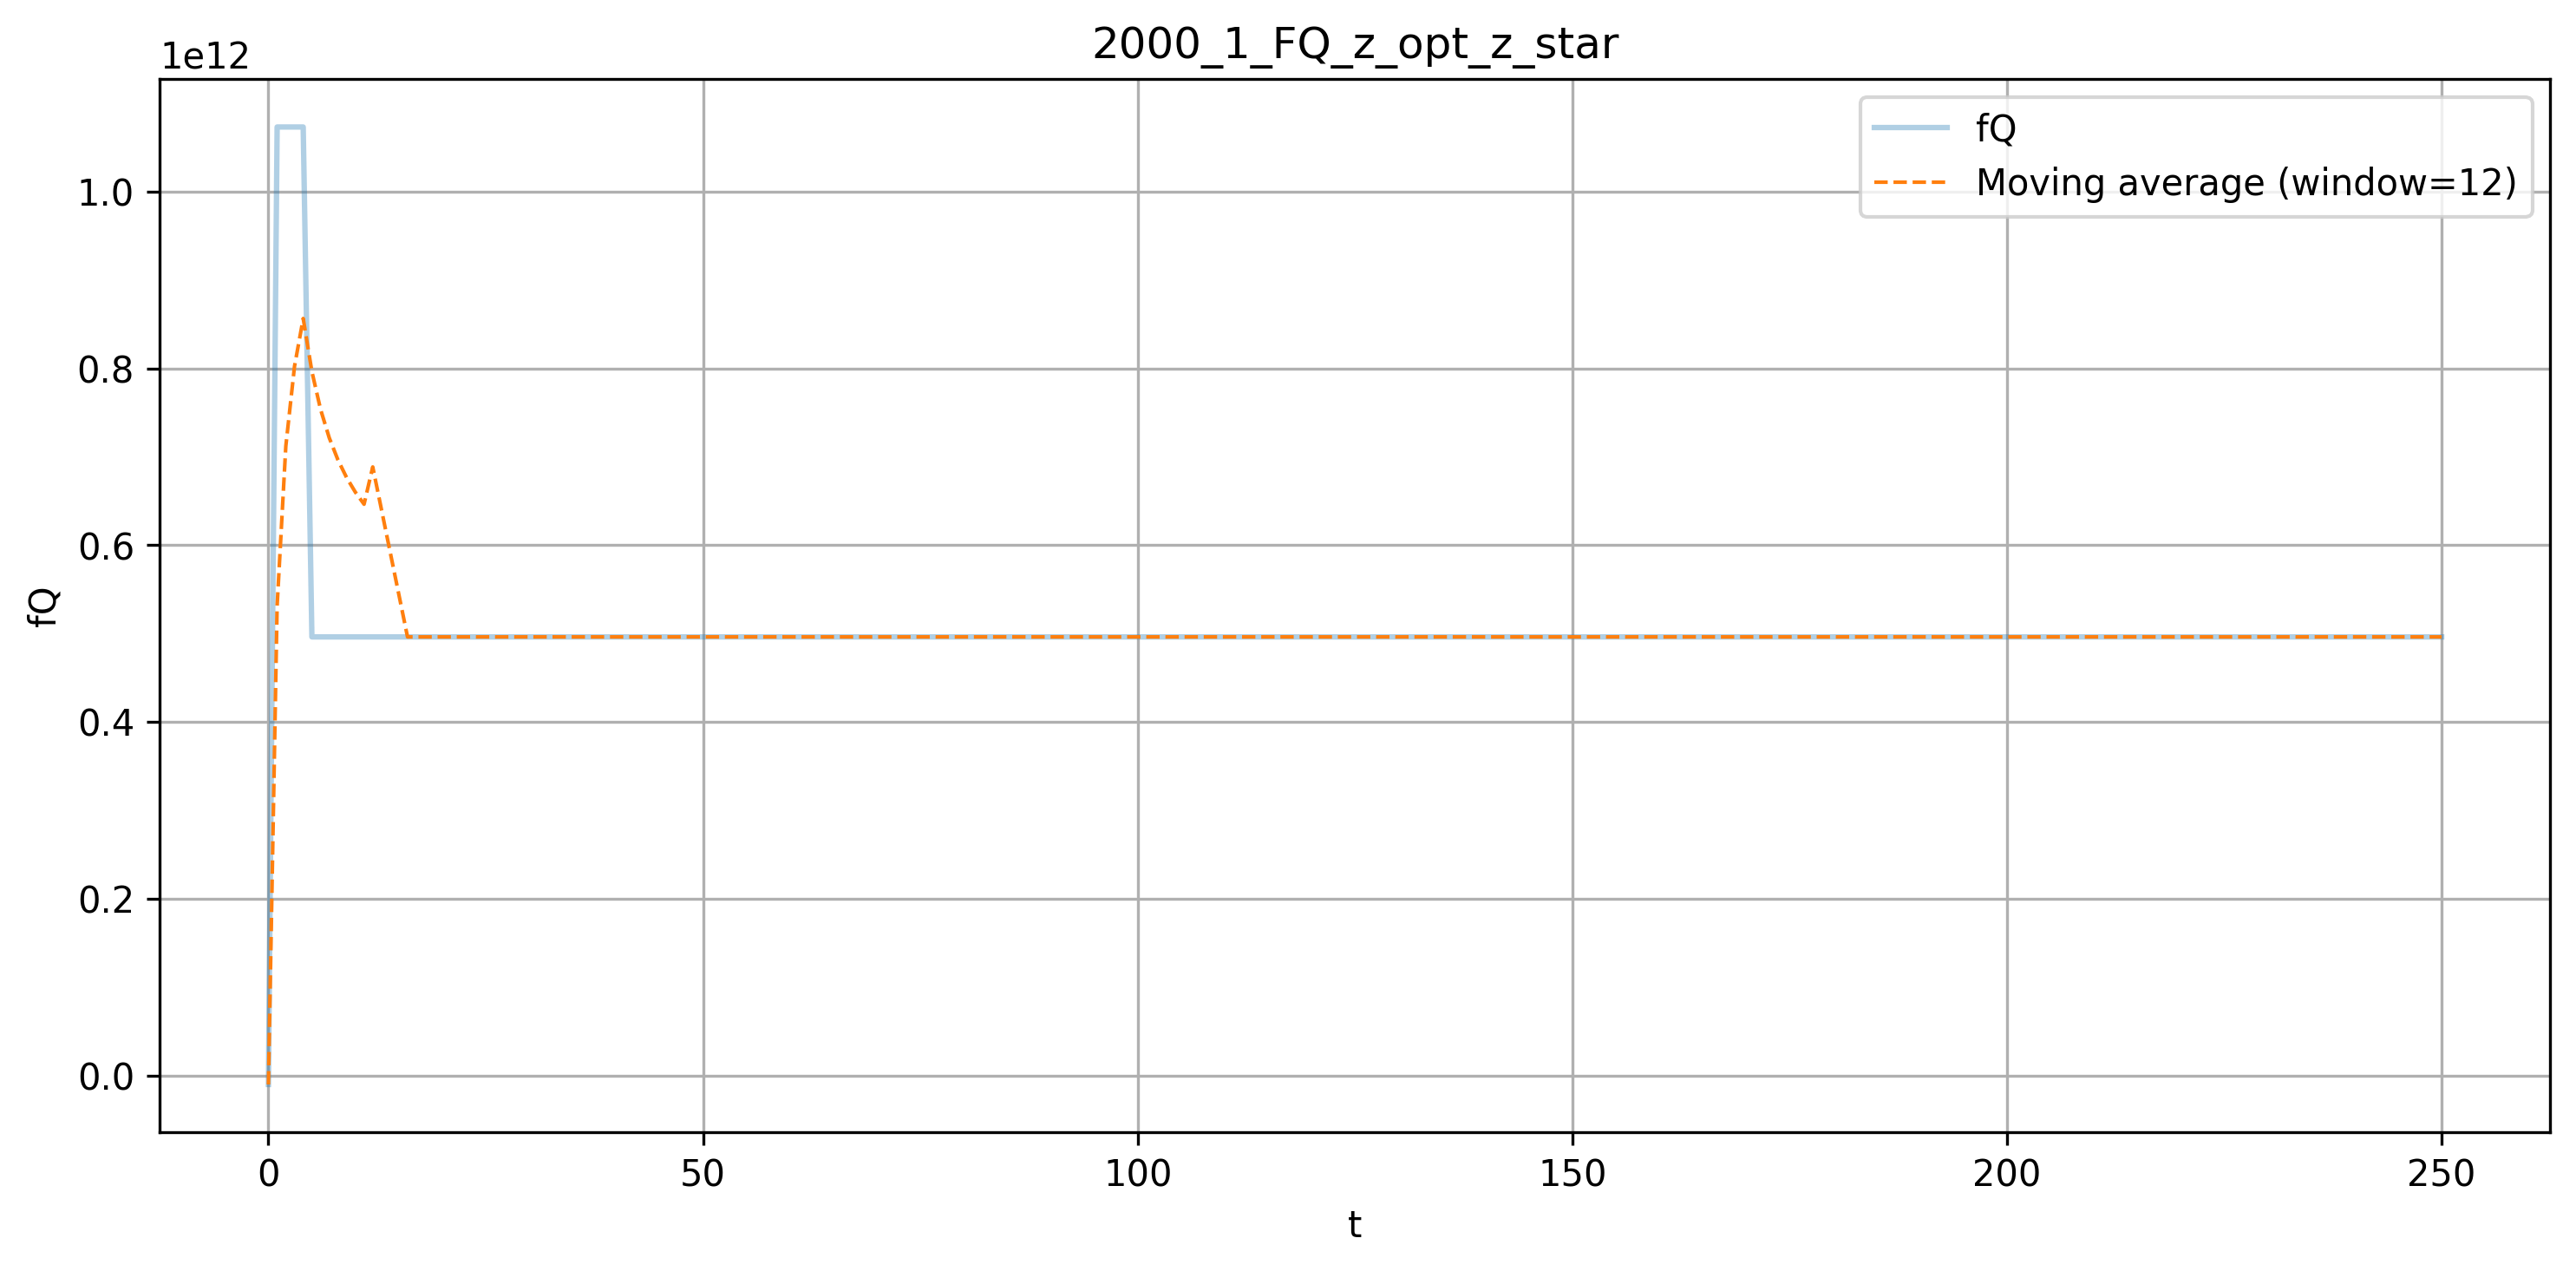
\includegraphics[width=\linewidth]{../Quantum-Annealing-for-solving-QUBO-Problems/test/Diagnostica_QALS/2/ksp_2/lambda_div_3/2000_1_FQ_z_opt_z_star.png}
    \caption{\(f_Q(z_\star)\) con \(\lambda_2\)}
    \label{fig:fQ-zstar-lambda2}
\end{subfigure}
\hfill
\begin{subfigure}{0.495\textwidth}
    \centering
    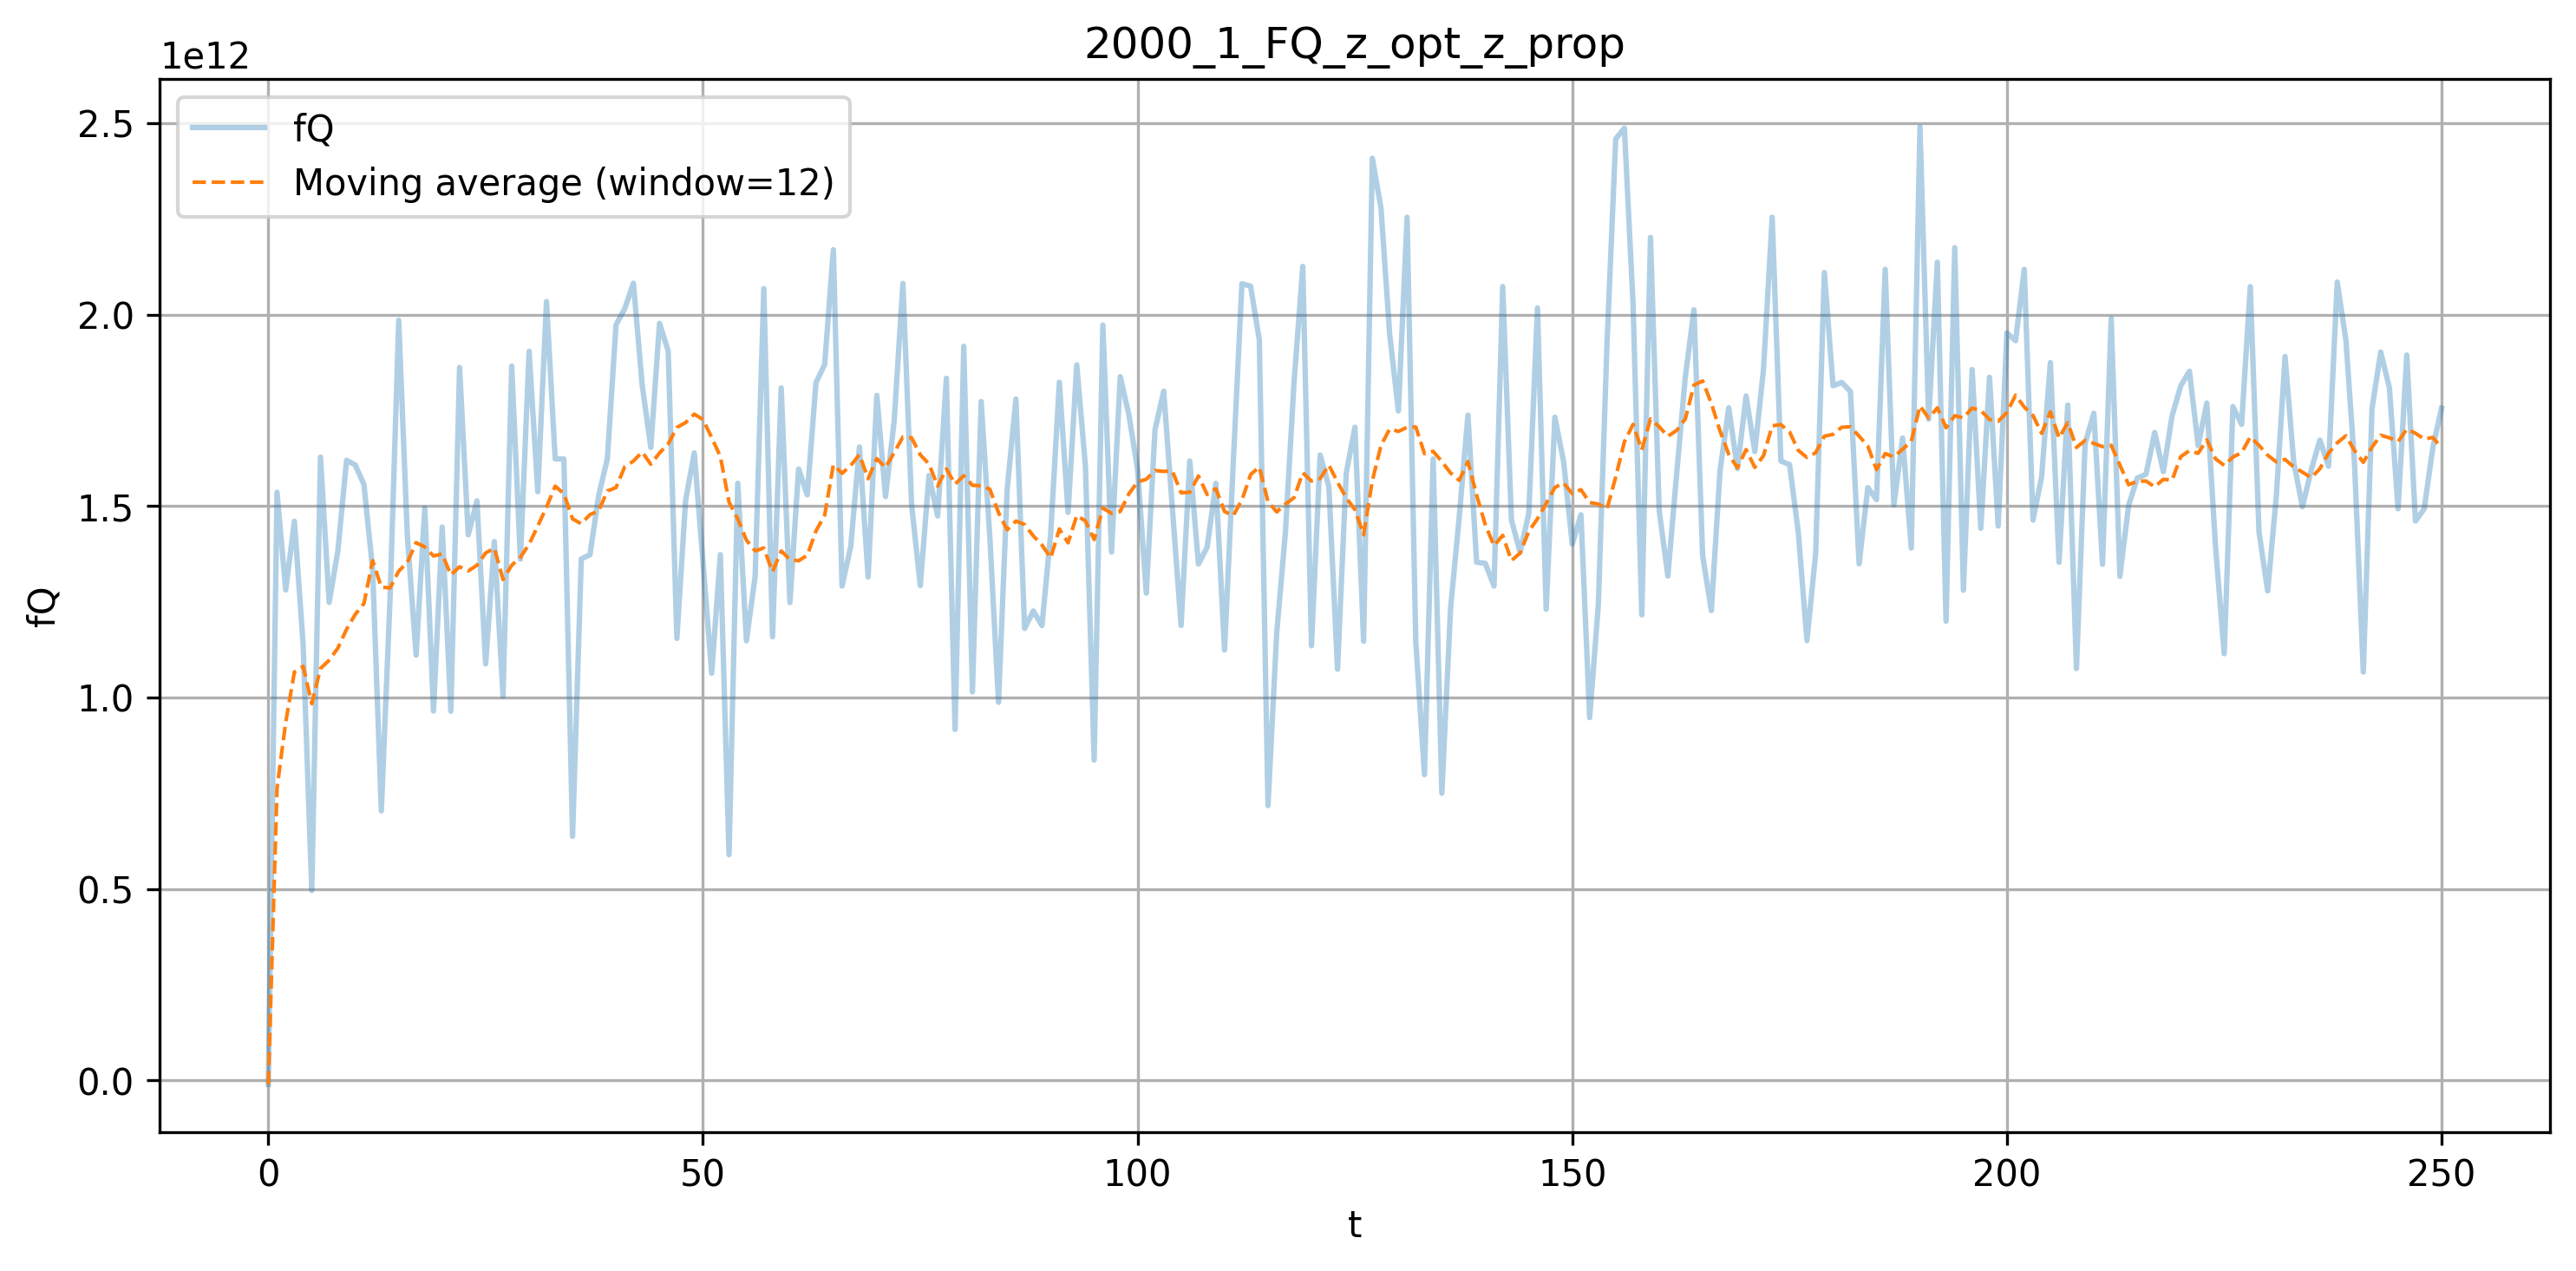
\includegraphics[width=\linewidth]{../Quantum-Annealing-for-solving-QUBO-Problems/test/Diagnostica_QALS/2/ksp_2/lambda_div_3/2000_1_FQ_z_opt_z_prop.png}
    \caption{\(f_Q(z_t)\) con \(\lambda_2\)}
    \label{fig:fQ-zt-lambda2}
\end{subfigure}
\label{fig:confronto-hamming-ksp22}
\end{figure}

\begin{figure}[H]
\centering
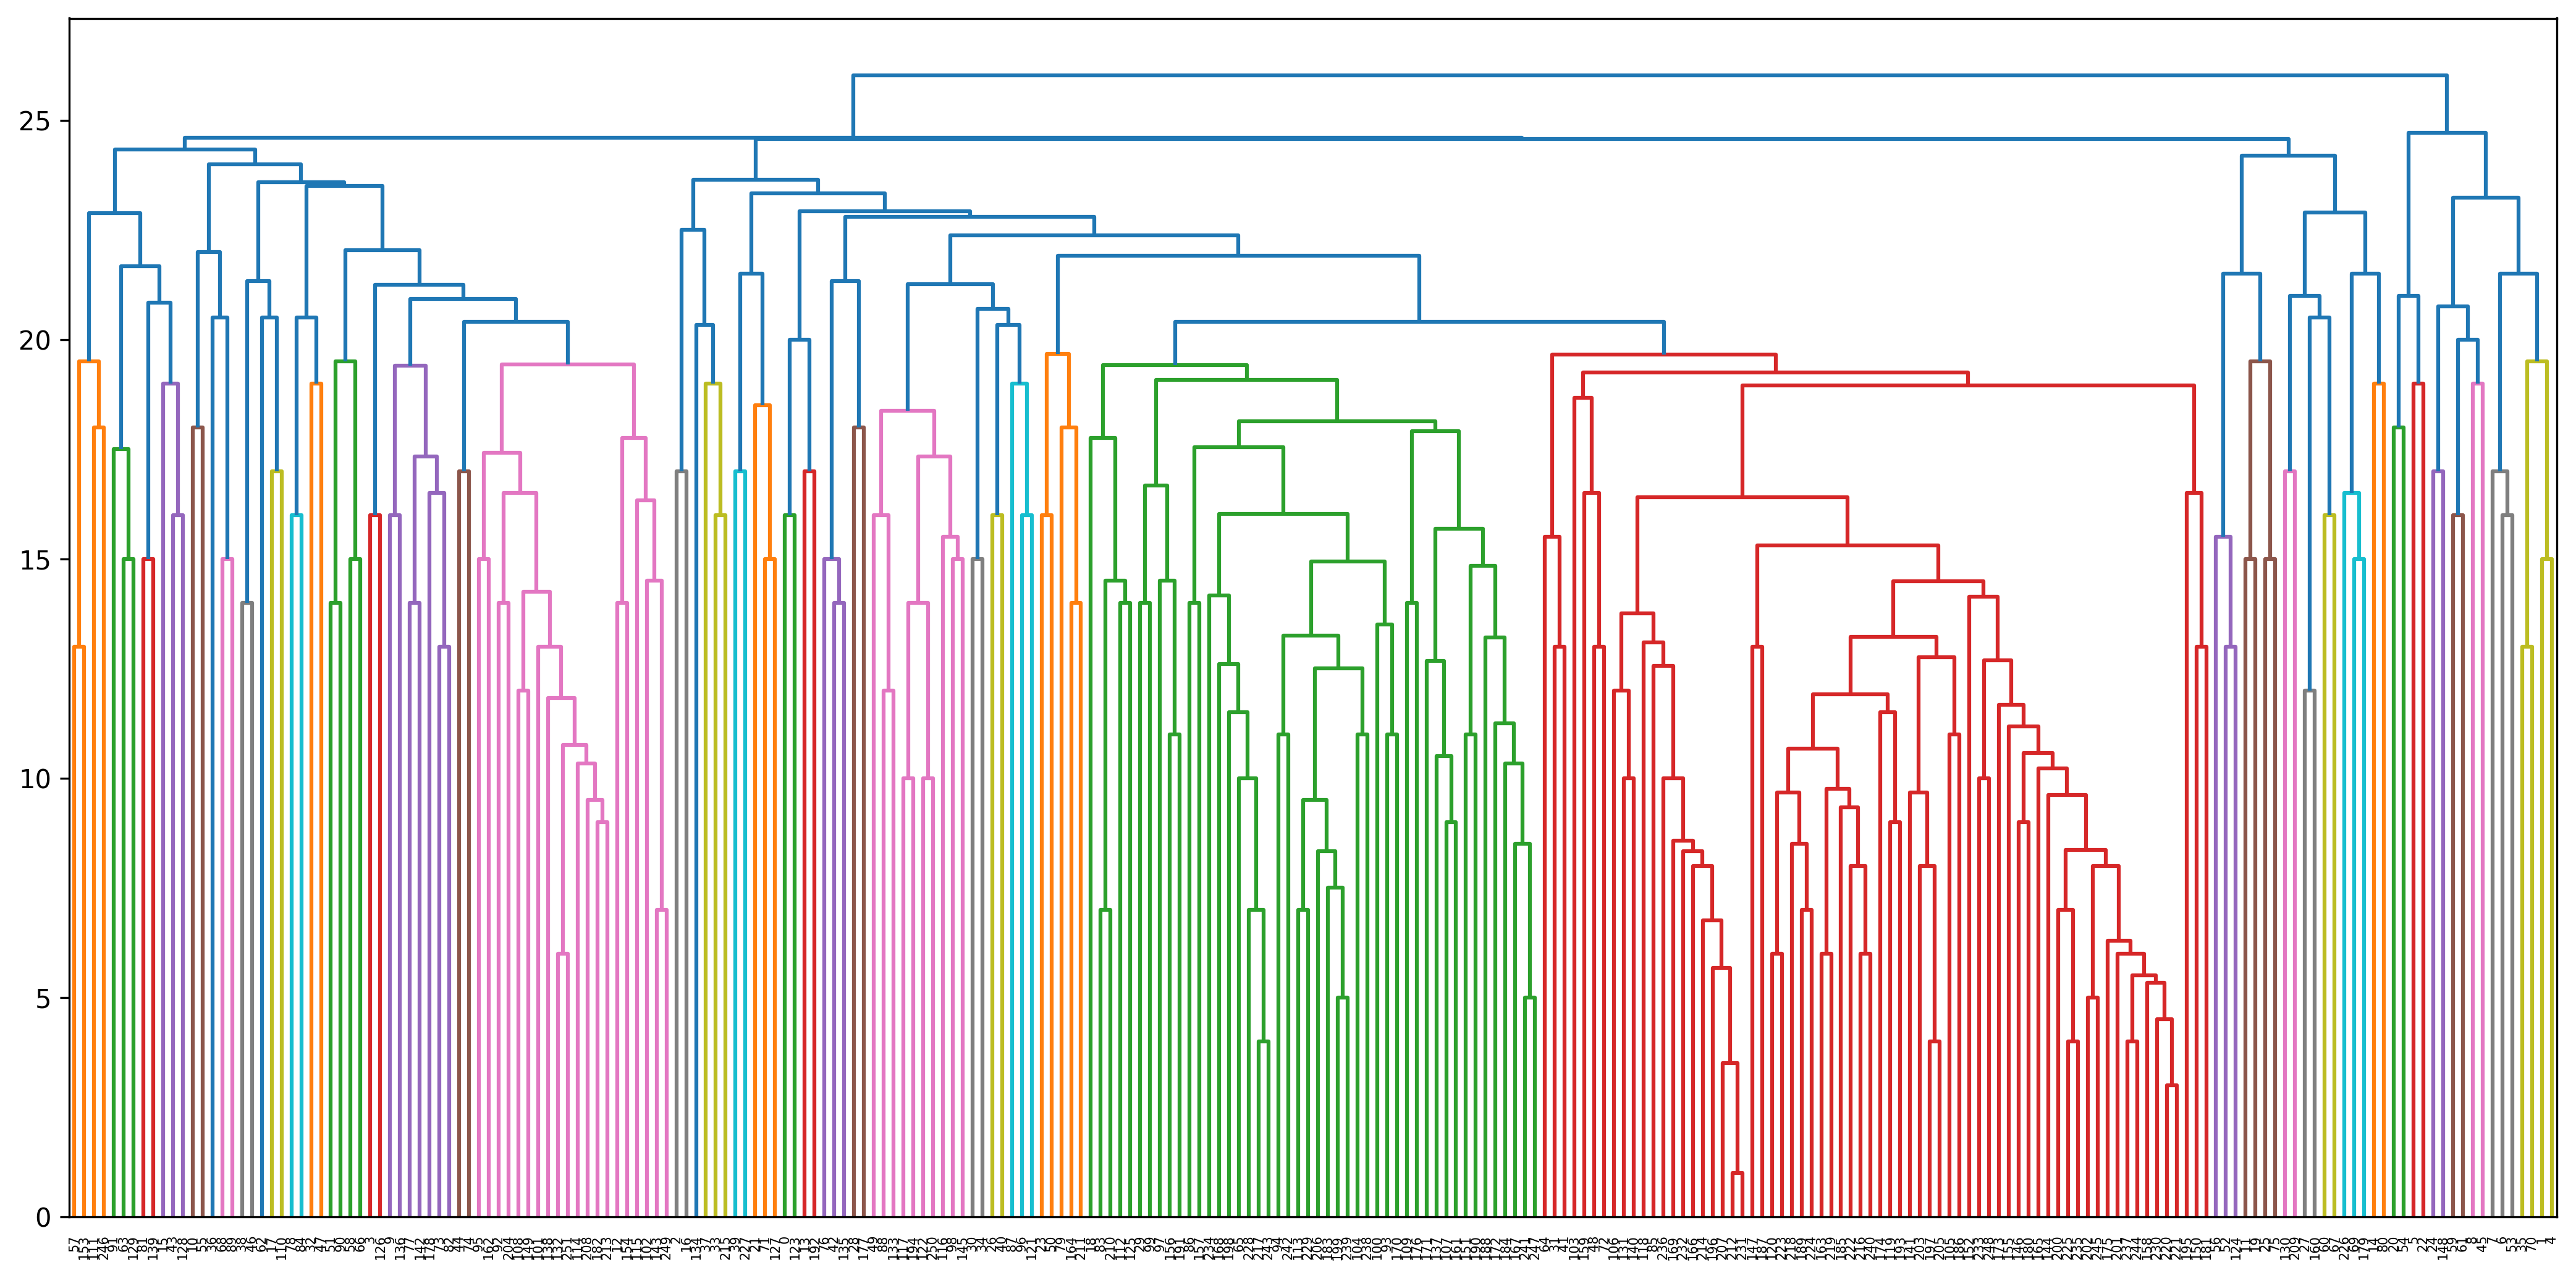
\includegraphics[width=\linewidth]{../Quantum-Annealing-for-solving-QUBO-Problems/test/Diagnostica_QALS/2/ksp_2/lambda_div_3/dendrogram_2000_1.png}
\caption{Agglomerative Clustering Dendogram}
\label{fig:AgglomerativeClustering-ksp2}
\end{figure}

\subsection{Riassunto dati}

\begin{table}[h]
\centering
\begin{tabular}{lccc|ccc}
\hline
& \multicolumn{3}{c|}{\(\boldsymbol{\lambda_1}\)}
& \multicolumn{3}{c}{\(\boldsymbol{\lambda_2}\)} \\
\cline{2-7}

\textbf{Istanza}
& \(\boldsymbol{f_Q}\)
& \(\boldsymbol{N_{\mathrm{cluster}}}\)
& \(\boldsymbol{|C_{\max}|}\)
& \(\boldsymbol{f_Q}\)
& \(\boldsymbol{N_{\mathrm{cluster}}}\)
& \(\boldsymbol{|C_{\max}|}\) \\
\hline

\texttt{ksp\_1}
& -301.62
& 9
& 226
& -1454230.67
& 10
& 160 \\

\texttt{ksp\_3}
& 89157.79
& 29
& 73
& 4487337042.67
& 30
& 110 \\

\texttt{ksp\_2}
& 828636.47
& 46
& 90
& 496218019323.67
& 47
& 68 \\

\hline
\end{tabular}
\caption{Confronto del valore obiettivo e delle caratteristiche del
clustering utilizzando \(\lambda_1\) e \(\lambda_2\).}
\label{tab:clustering-lambda-confronto-2}
\end{table}

\subsection{Interpretazione dei risultati}
I risultati mostrano che QALS mantiene una certa capacità di generare configurazioni differenti, ma tale esplorazione non si traduce necessariamente in 
un miglioramento della soluzione corrente o nell'avvicinamento alla soluzione ottima.

In tutti e tre i test case, la distanza:
\[
d_H(z_\star^{old},z_\star^{new})
\]
assume valori diversi da zero soprattutto nelle prime iterazioni, per poi diventare quasi sempre nulla. Questo comportamento indica che QALS modifica
la soluzione corrente soprattutto nella fase iniziale dell'esplorazione, ma successivamente tende a mantenere la stessa configurazione per intervalli molto lunghi, 
ma ciò dipende dal parametro che decide la probbabilità di accettare una nuova soluzione. 
I picchi isolati osservabili in alcune esecuzioni corrispondono all'accettazione occasionale di una nuova soluzione, eventualmente anche peggiorativa, 
prevista dal meccanismo probabilistico dell'algoritmo.
Inoltre se considerassimo:
\[
d_H(z_{opt},z_\star)
\qquad
f_Q(z_\star)
\]
si nota che \(z_\star\) continui a dimuinuire ad ogni cambio.

Se ora prendessimo in considerazione le distanze:
\[
d_H(z_t,z_\star)
\]
in tutti i casi si puo vedere come tutte suggeriscano un'esplorazione variegata dello spazio delle soluzioni in quanto, in relazione ad ogni test case, le distanze oscillano
in modo significativo mantenendo un valore superiore alla metà del numero di elementi per ogni test case. 

In particolar nel test case \texttt{ksp\_3} si noti come mano a mano che l'esecuzione procede, la distanza diminuisca, o per lo meno si appiattisca, pattern che però non si ripete nè 
in \texttt{ksp\_1} nè in \texttt{ksp\_2} il che può essere giustificato dal comportamento probabilistico dell'algoritmo.

Infine integrando con:
\[
f_Q(z_t)
\qquad
dendogram
\]
si può concludere che QALS abbia si una certa capacità di esplorazione, ma che questa si concentri prevalentemente in alcune regione dello spazio. Questo comportamento è meno evidente
utilizzando \(\lambda_2 = \frac{\sum_{i=1}^{n} p_i}{3}.\)

Nel complesso, la diagnostica mostra quindi che QALS non è privo di esplorazione. Le soluzioni candidate continuano a variare e, soprattutto nei problemi di dimensione maggiore, 
risultano esere più distribuite tra cluster. Il problema principale non sembra essere l'assenza di movimento nello spazio delle soluzioni, bensì la scarsa efficacia della direzione seguita
dalla ricerca. QALS esplora molte configurazioni, ma tende a concentrarsi nelle stesse regioni e distanti dall'ottimo; inoltre, dopo le prime iterazioni, modifica raramente la soluzione corrente.

\clearpage
\section{Decay Factor}

\subsection{ksp\_1}

\begin{table}[h]
\centering
\begin{tabular}{lcc}
\hline
\textbf{Metrica} & \(\lambda_1\) & \(\lambda_2\) \\
\hline
Numero cluster & 8 & 13 \\
Dimensione cluster massimo & 225 & 140 \\
Cluster z best & 3 & 9 \\
Single clusters & 0 & 0 \\
Medoid cluster massimo & 
\([0\,0\,0\,1\,0\,0\,0\,0\,0\,0]\) &
\([1\,1\,0\,1\,1\,1\,0\,0\,1\,1]\) \\
\(f_Q\) medoid & -84.4 & 12521312.0 \\
Profit medoid & 25 & 256 \\
Weight medoid & 68 & 414 \\
\hline
\(f_Q\) Min Found QALS & -267.3 & -1454230.67 \\
Profit Found QALS & 214 & 172 \\
Weight Found QALS & 146 & 104 \\
\hline
\(f_Q\) Min Found NO QALS & -330.85 & -1455540.67 \\
Profit Found NO QALS & 302 & 198 \\
Weight Found NO QALS & 177 & 101 \\
\hline
\end{tabular}

\caption{Confronto dei risultati ottenuti con QALS e senza QALS.}
\label{tab:confronto-qals-noqals}
\end{table}

\begin{figure}[H]
\centering
\begin{subfigure}{0.495\textwidth}
    \centering
    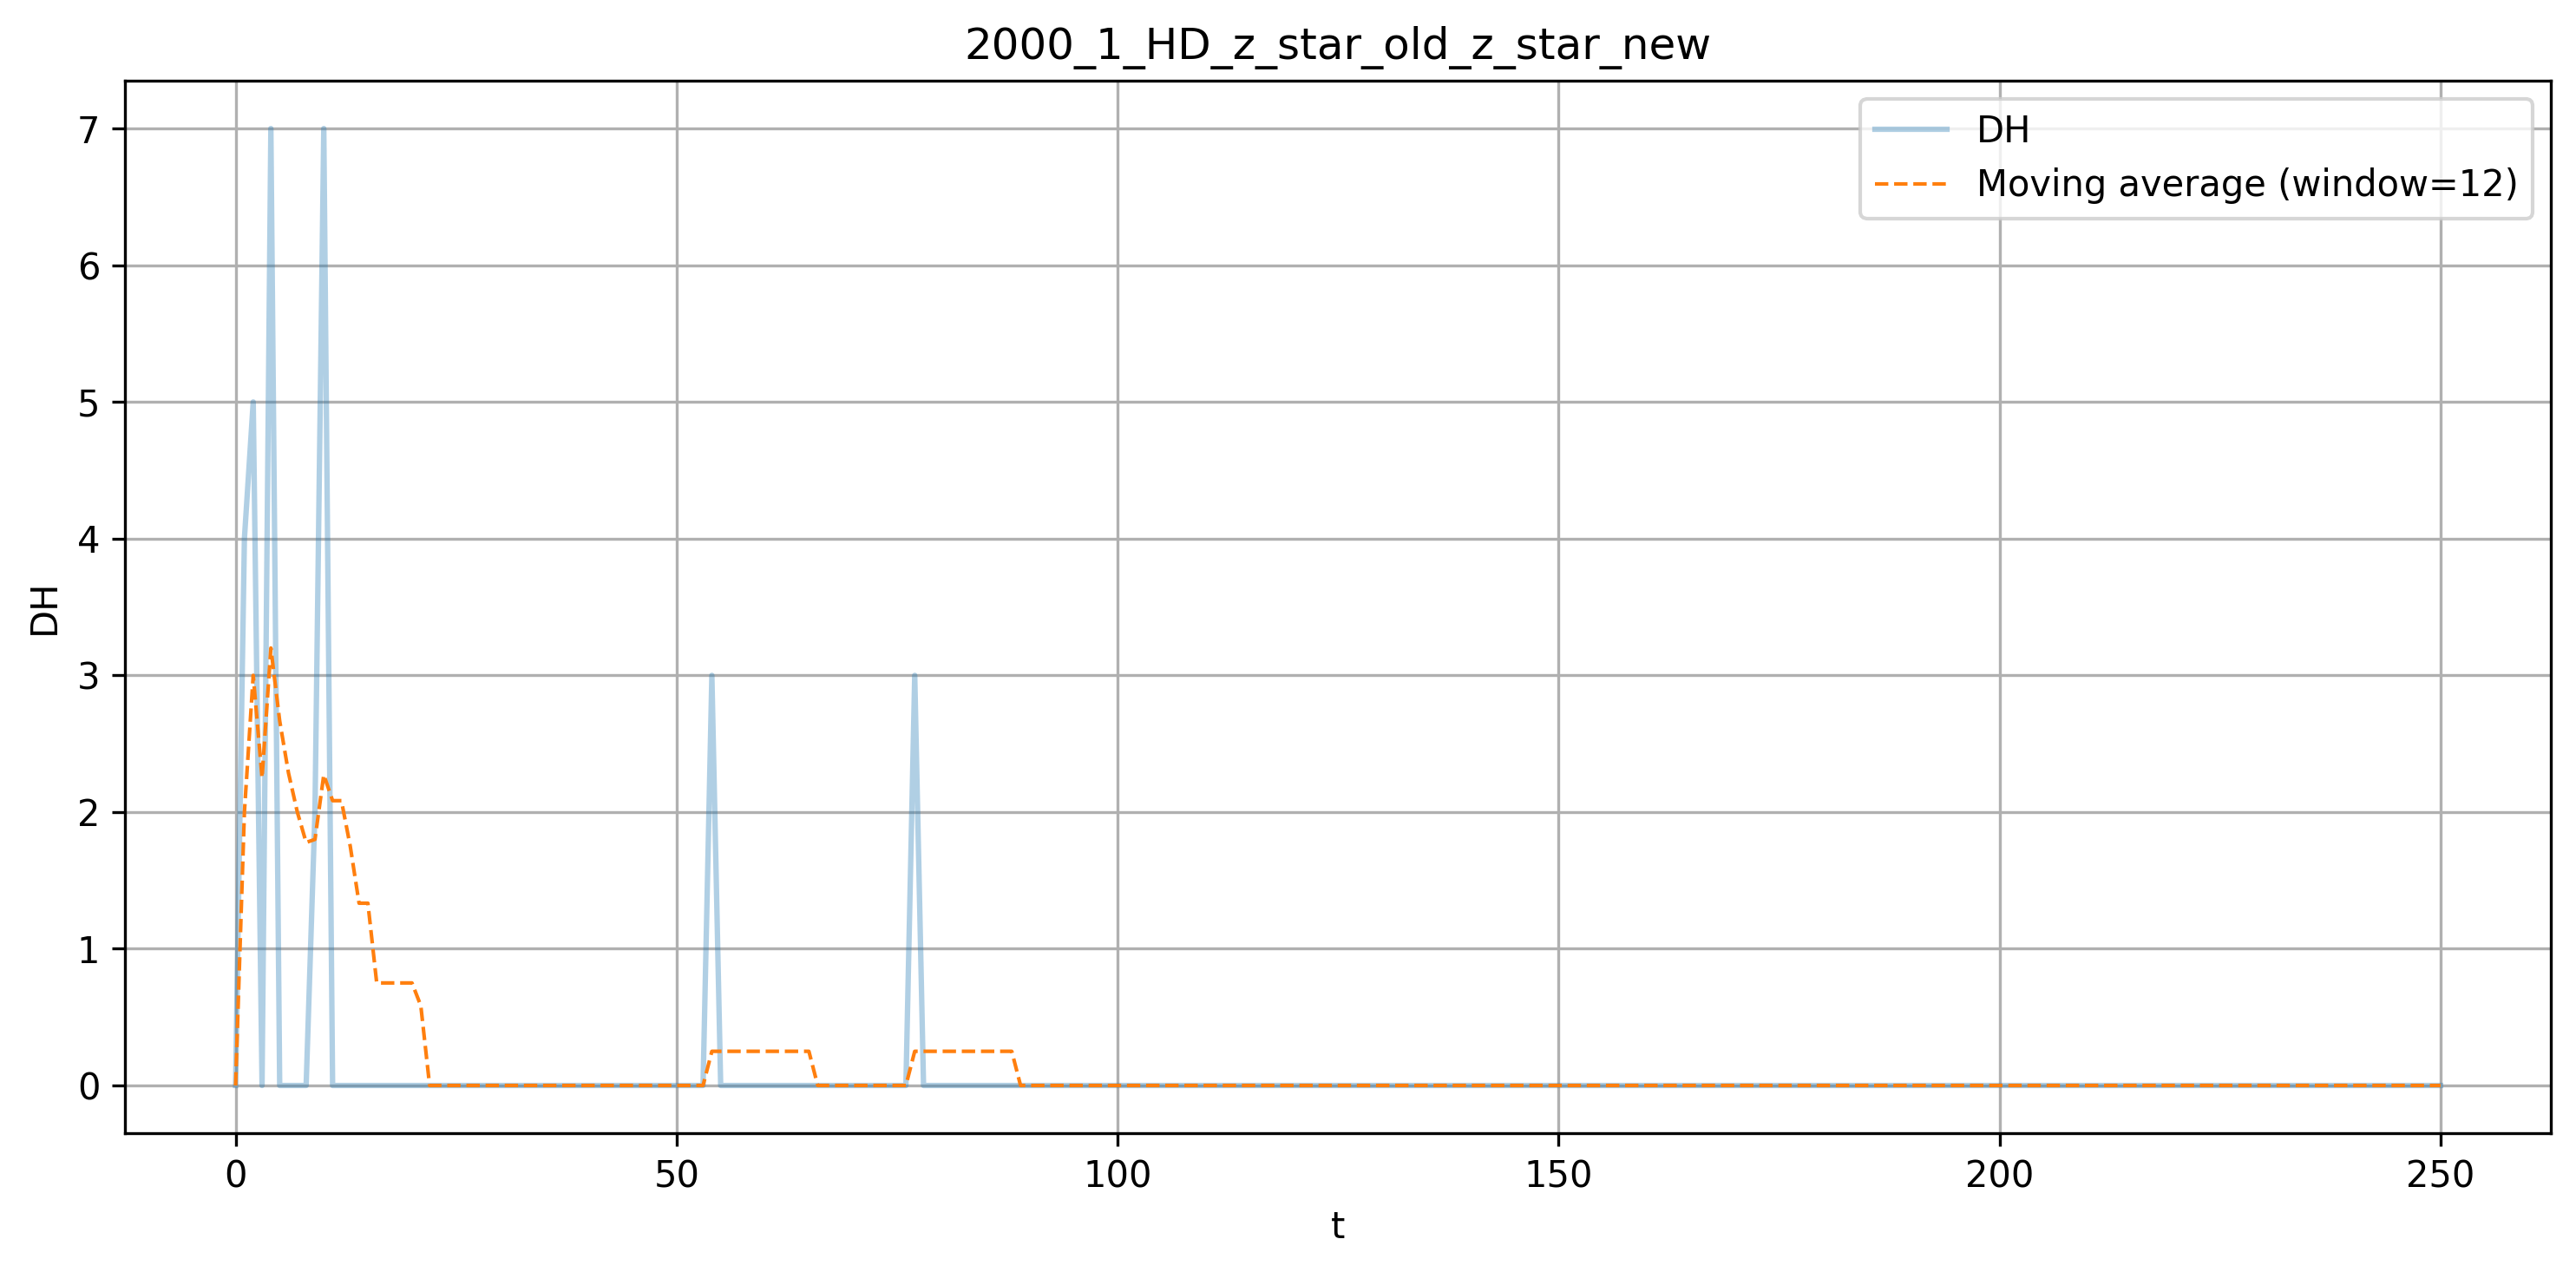
\includegraphics[width=\linewidth]{../Quantum-Annealing-for-solving-QUBO-Problems/test/Diagnostica_QALS/2/Decay_factor/ksp_1/lambda_650_dot_C/2000_1_HD_z_star_old_z_star_new.png}
    \caption{\(d_H(z_\star^{old}, z_\star^{new})\) con \(\lambda_1\)}
    \label{fig:hd-zstarold-zstarnew-lambda1}
\end{subfigure}
\hfill
\begin{subfigure}{0.495\textwidth}
    \centering
    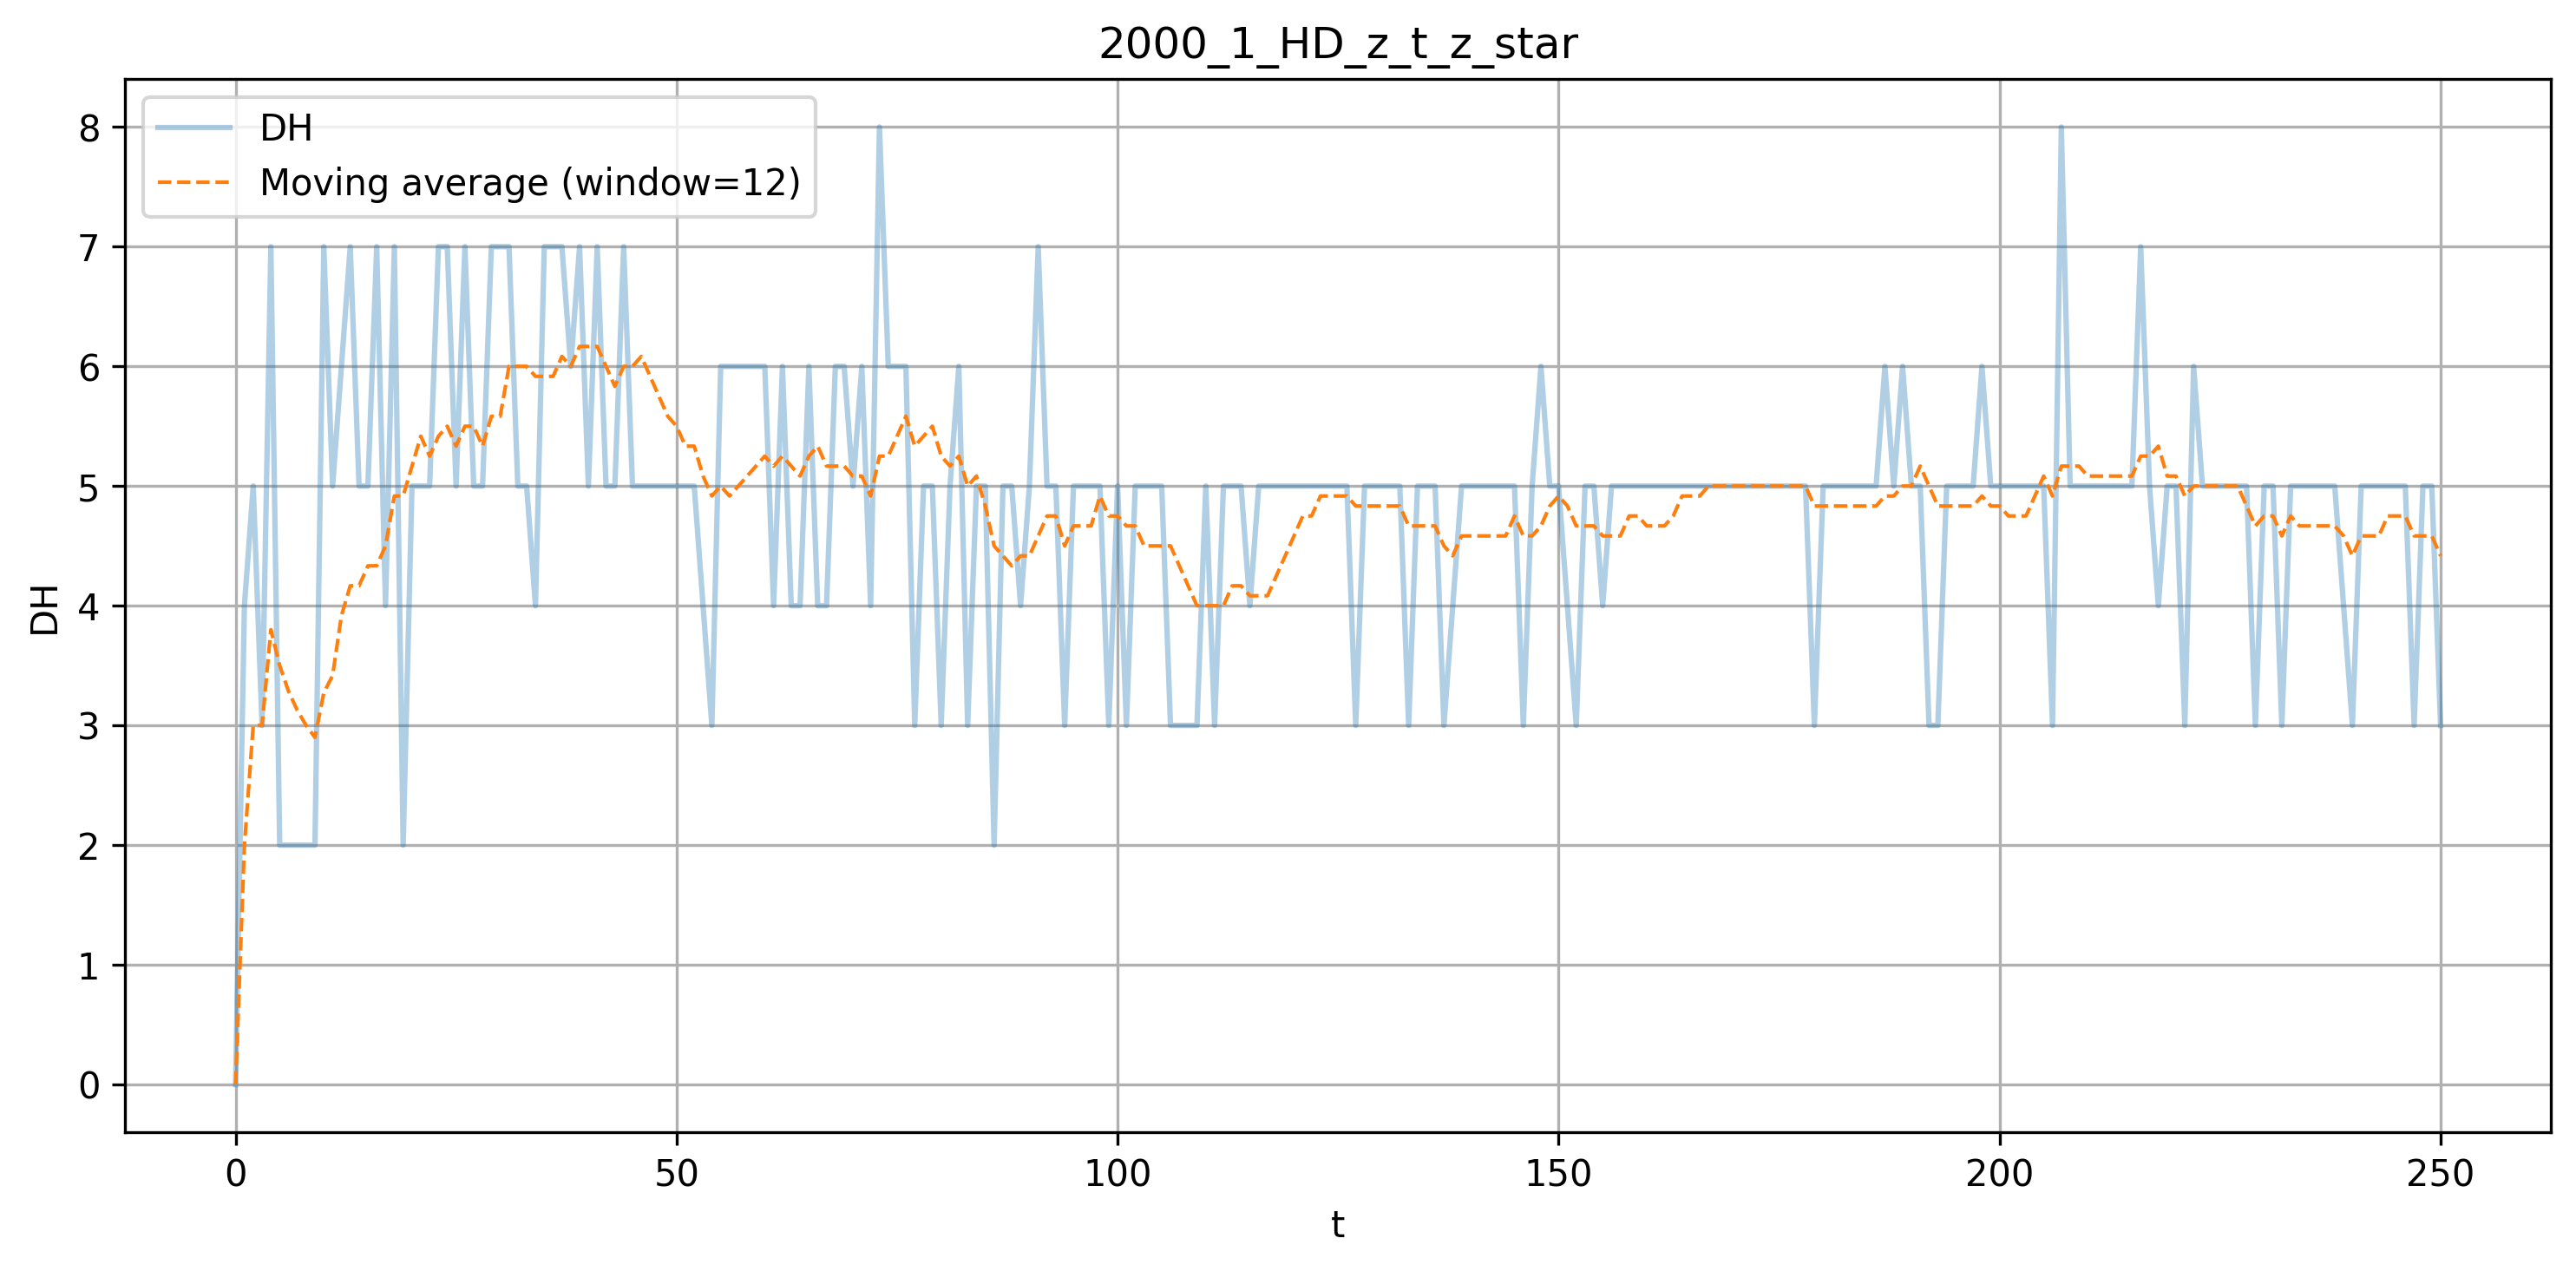
\includegraphics[width=\linewidth]{../Quantum-Annealing-for-solving-QUBO-Problems/test/Diagnostica_QALS/2/Decay_factor/ksp_1/lambda_650_dot_C/2000_1_HD_z_t_z_star.png}
    \caption{\(d_H(z_t, z_\star)\) con \(\lambda_1\)}
    \label{fig:hd-zt-zstar-lambda1}
\end{subfigure}

\vspace{0.35cm}

\begin{subfigure}{0.495\textwidth}
    \centering
    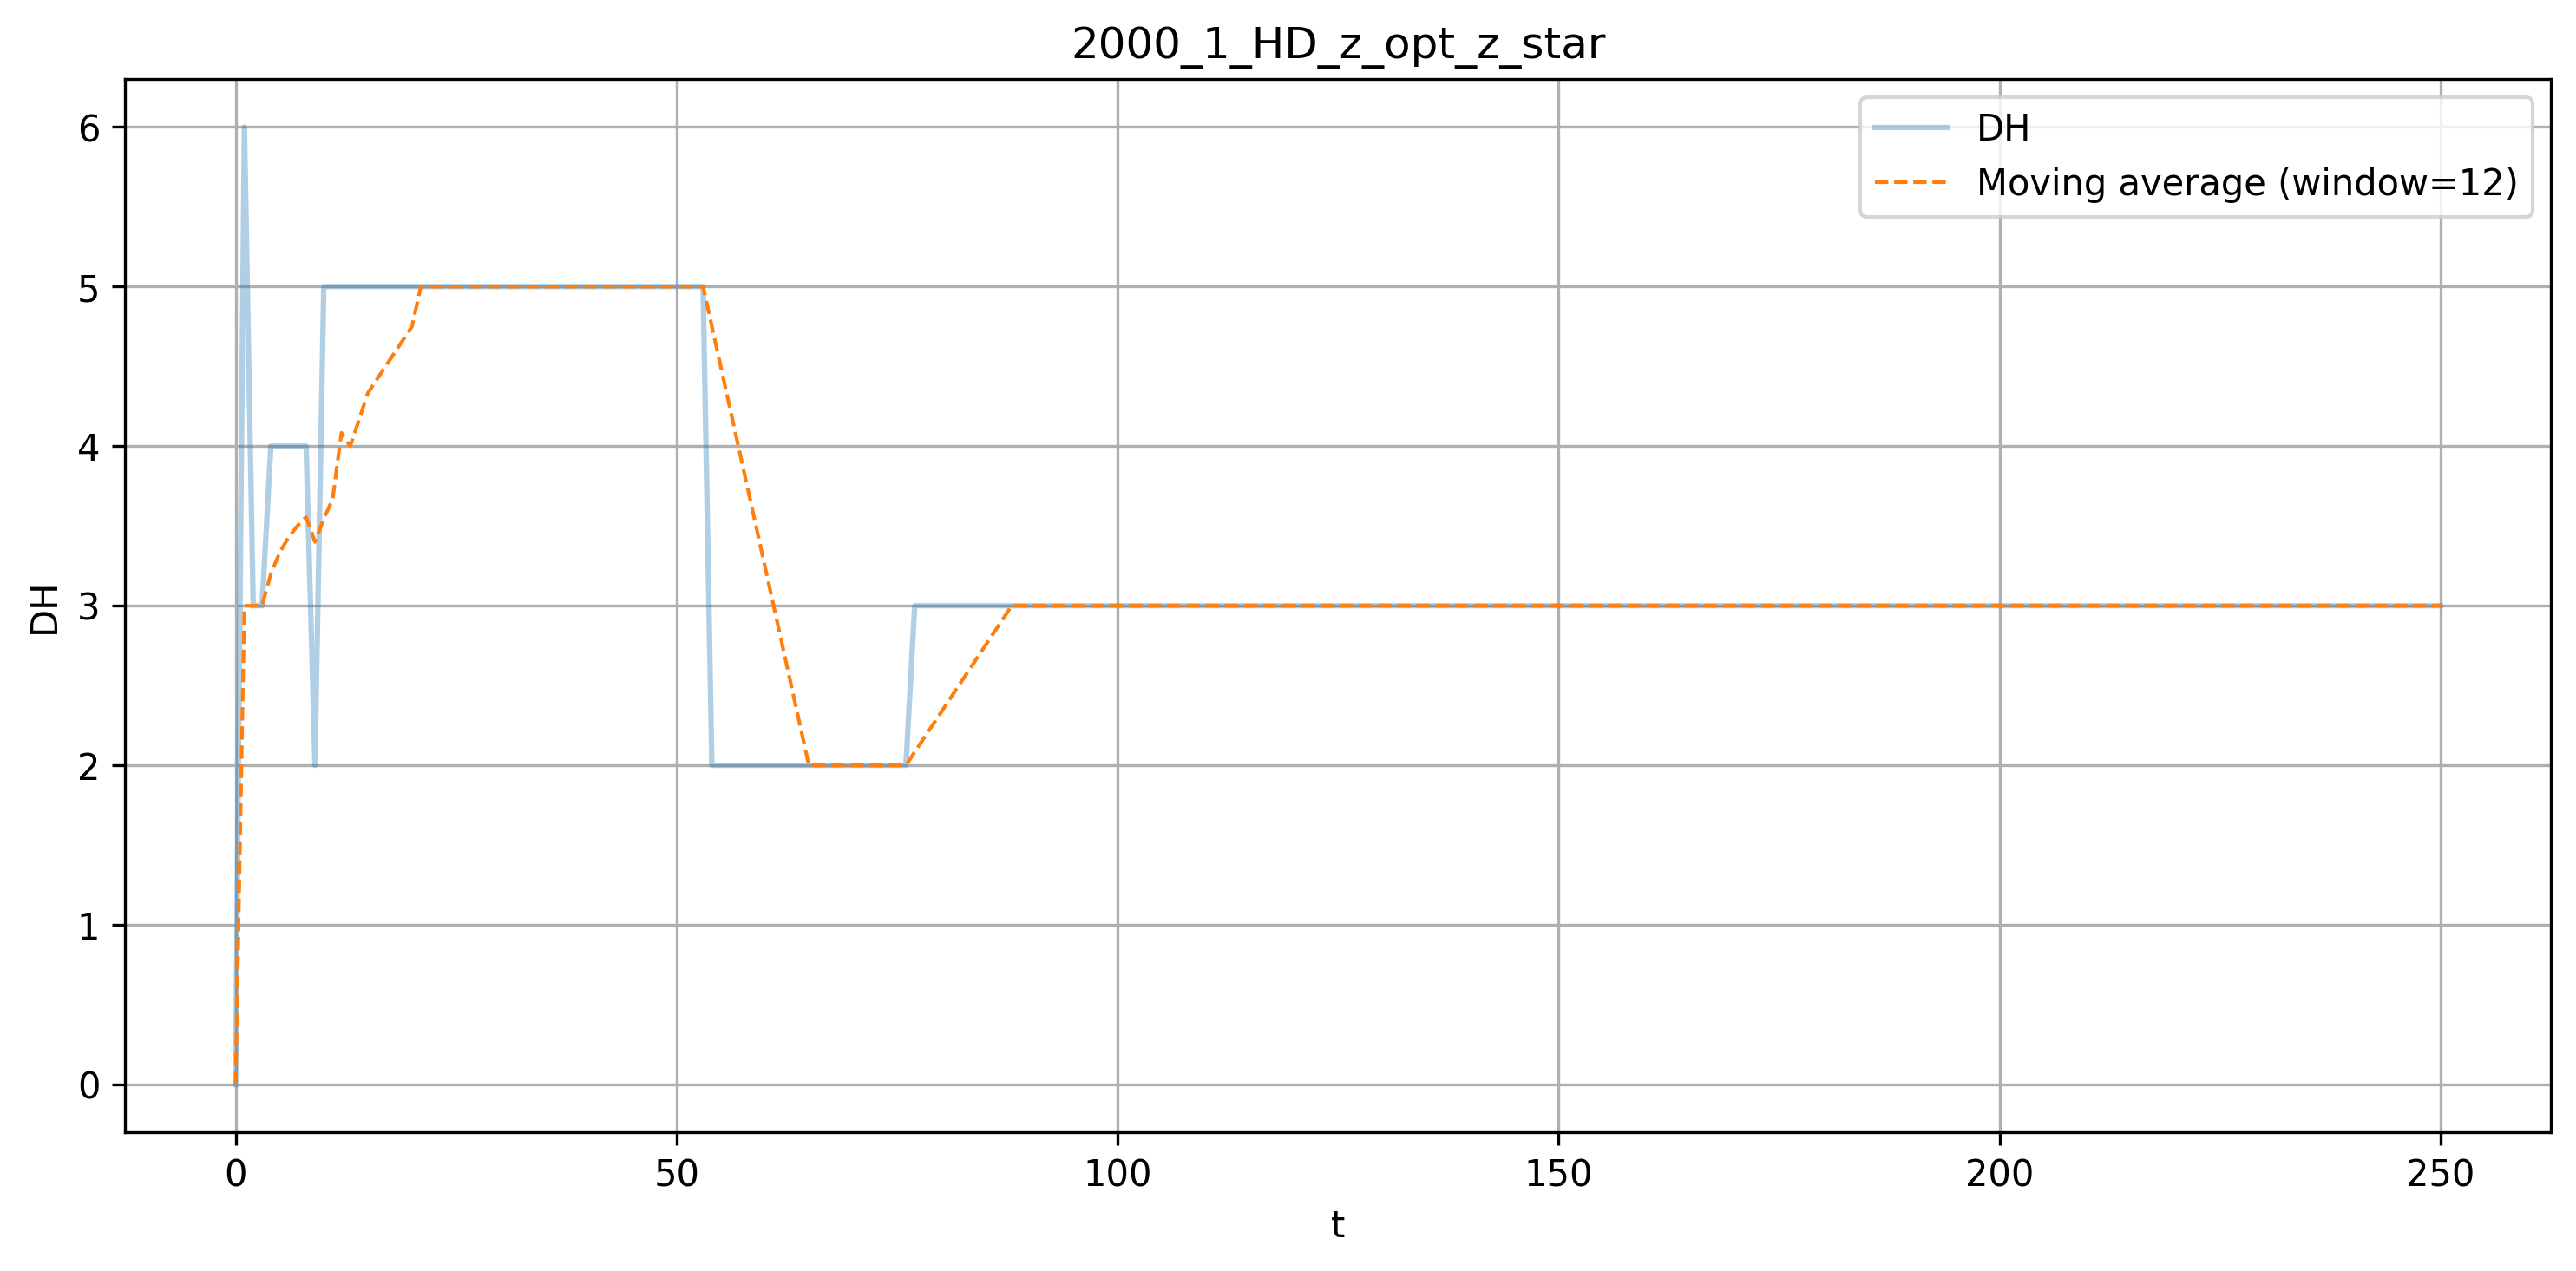
\includegraphics[width=\linewidth]{../Quantum-Annealing-for-solving-QUBO-Problems/test/Diagnostica_QALS/2/Decay_factor/ksp_1/lambda_650_dot_C/2000_1_HD_z_opt_z_star.png}
    \caption{\(d_H(z_{opt}, z_\star)\) con \(\lambda_1\)}
    \label{fig:hd-zopt-zstar-lambda1}
\end{subfigure}
\hfill
\begin{subfigure}{0.495\textwidth}
    \centering
    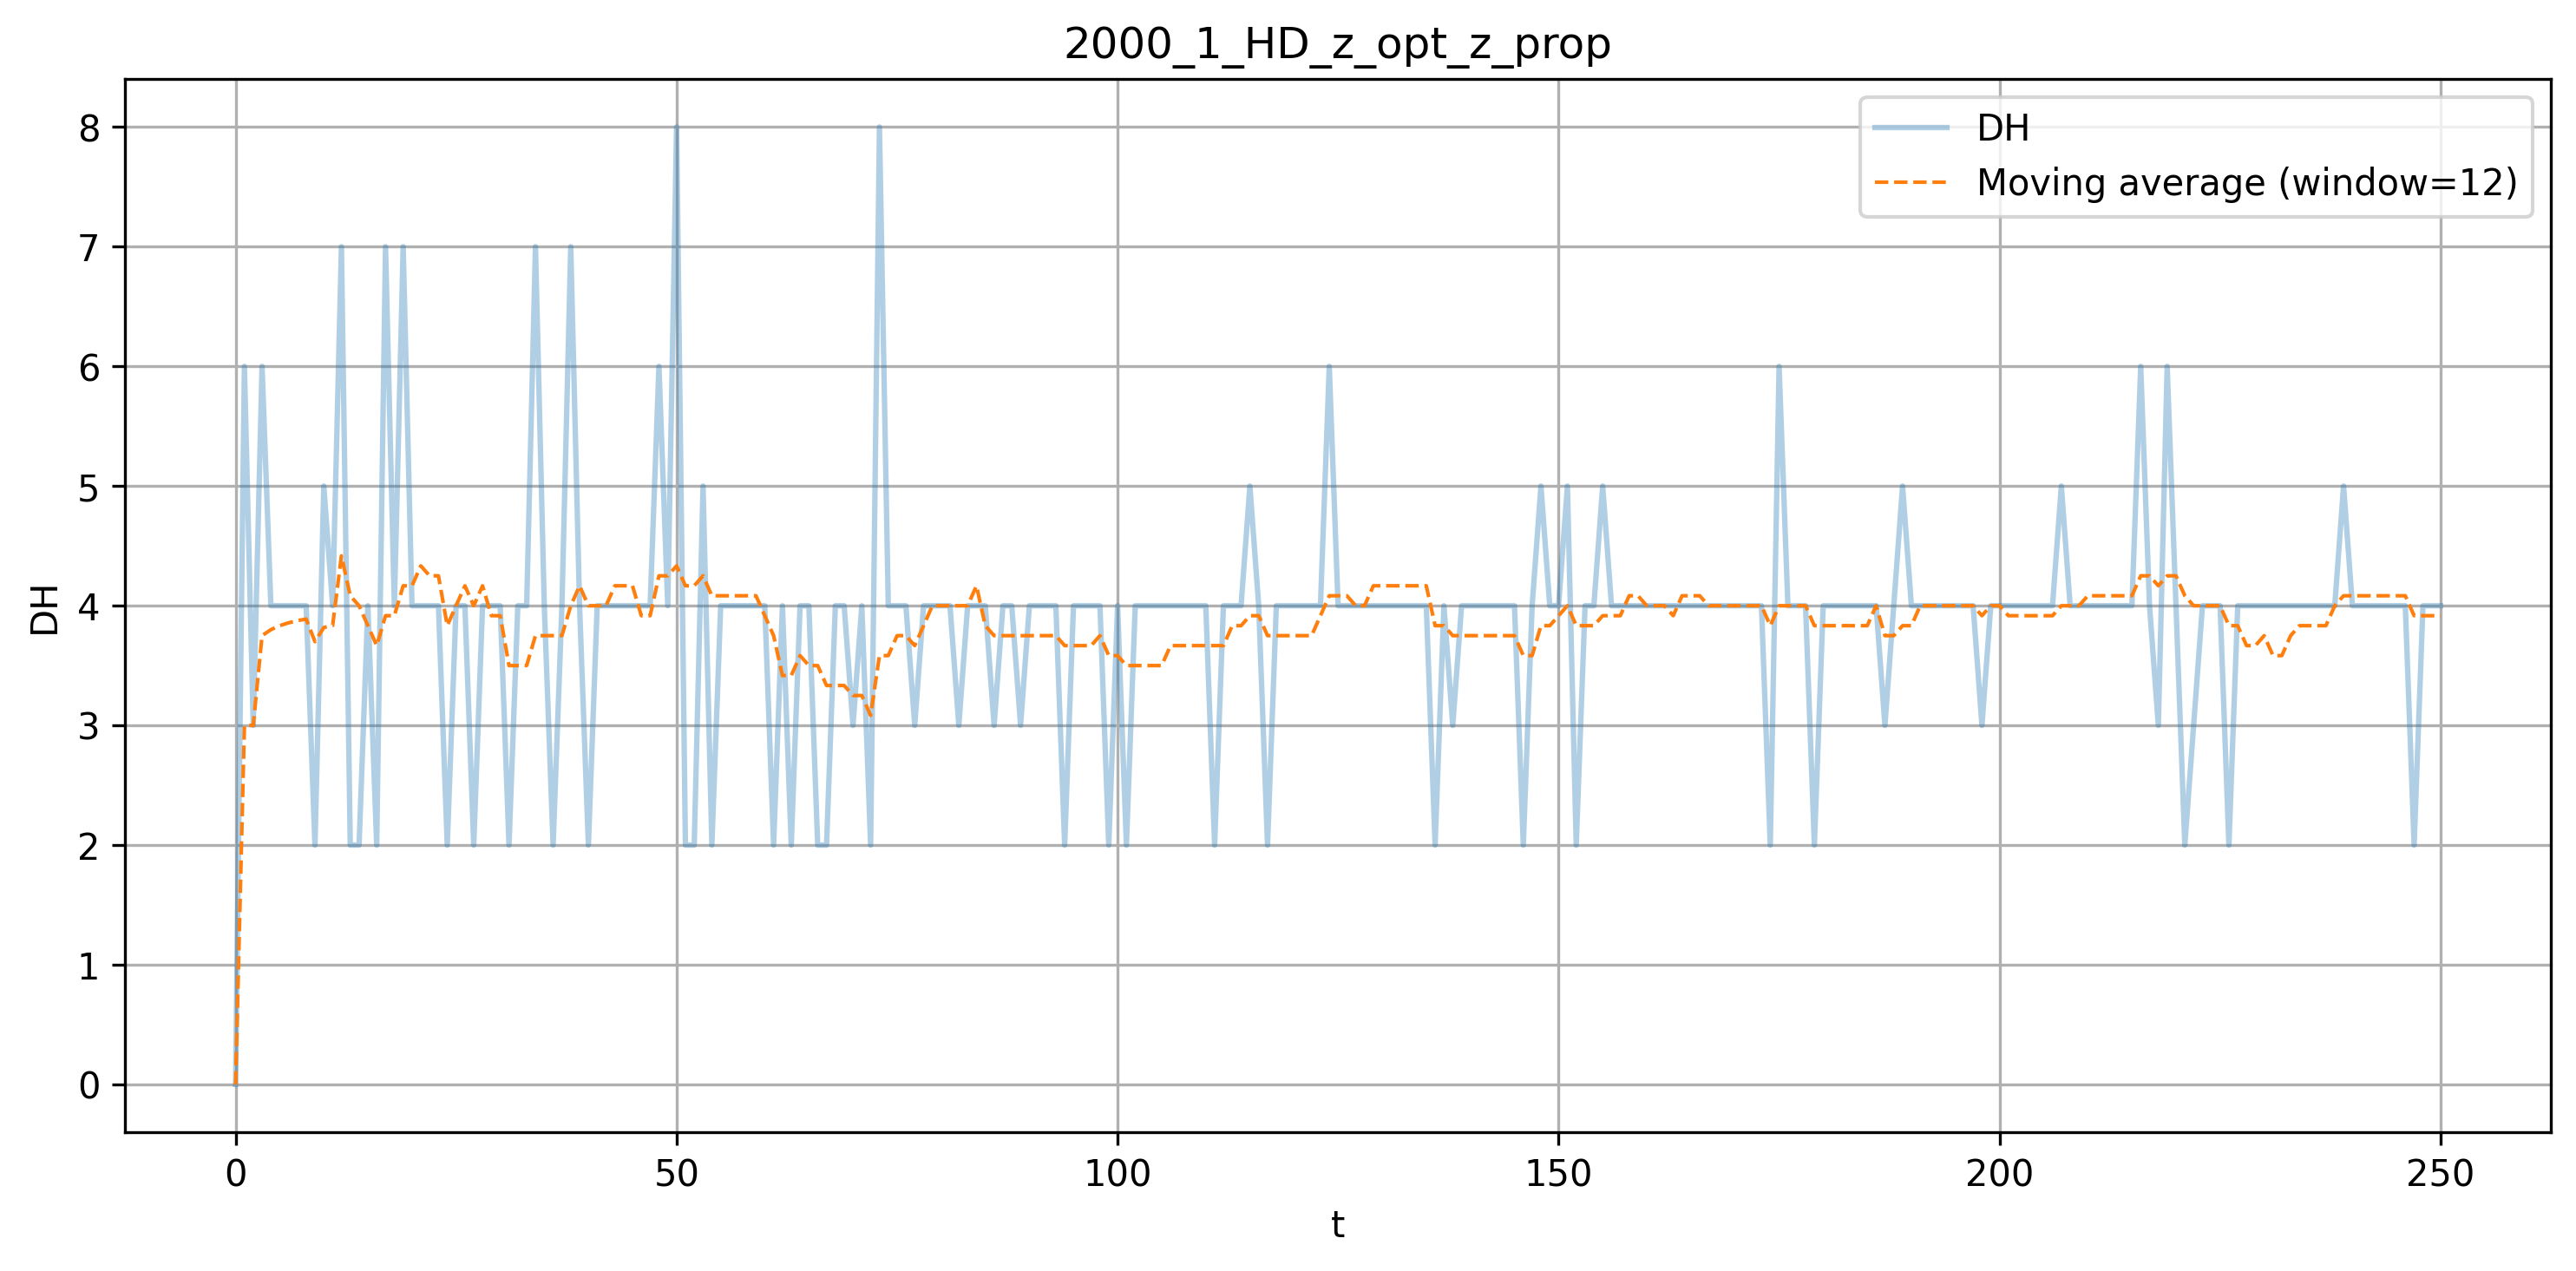
\includegraphics[width=\linewidth]{../Quantum-Annealing-for-solving-QUBO-Problems/test/Diagnostica_QALS/2/Decay_factor/ksp_1/lambda_650_dot_C/2000_1_HD_z_opt_z_prop.png}
    \caption{\(d_H(z_{opt}, z_t)\) con \(\lambda_1\)}
    \label{fig:hd-zopt-zt-lambda1}
\end{subfigure}

\vspace{0.35cm}

\begin{subfigure}{0.495\textwidth}
    \centering
    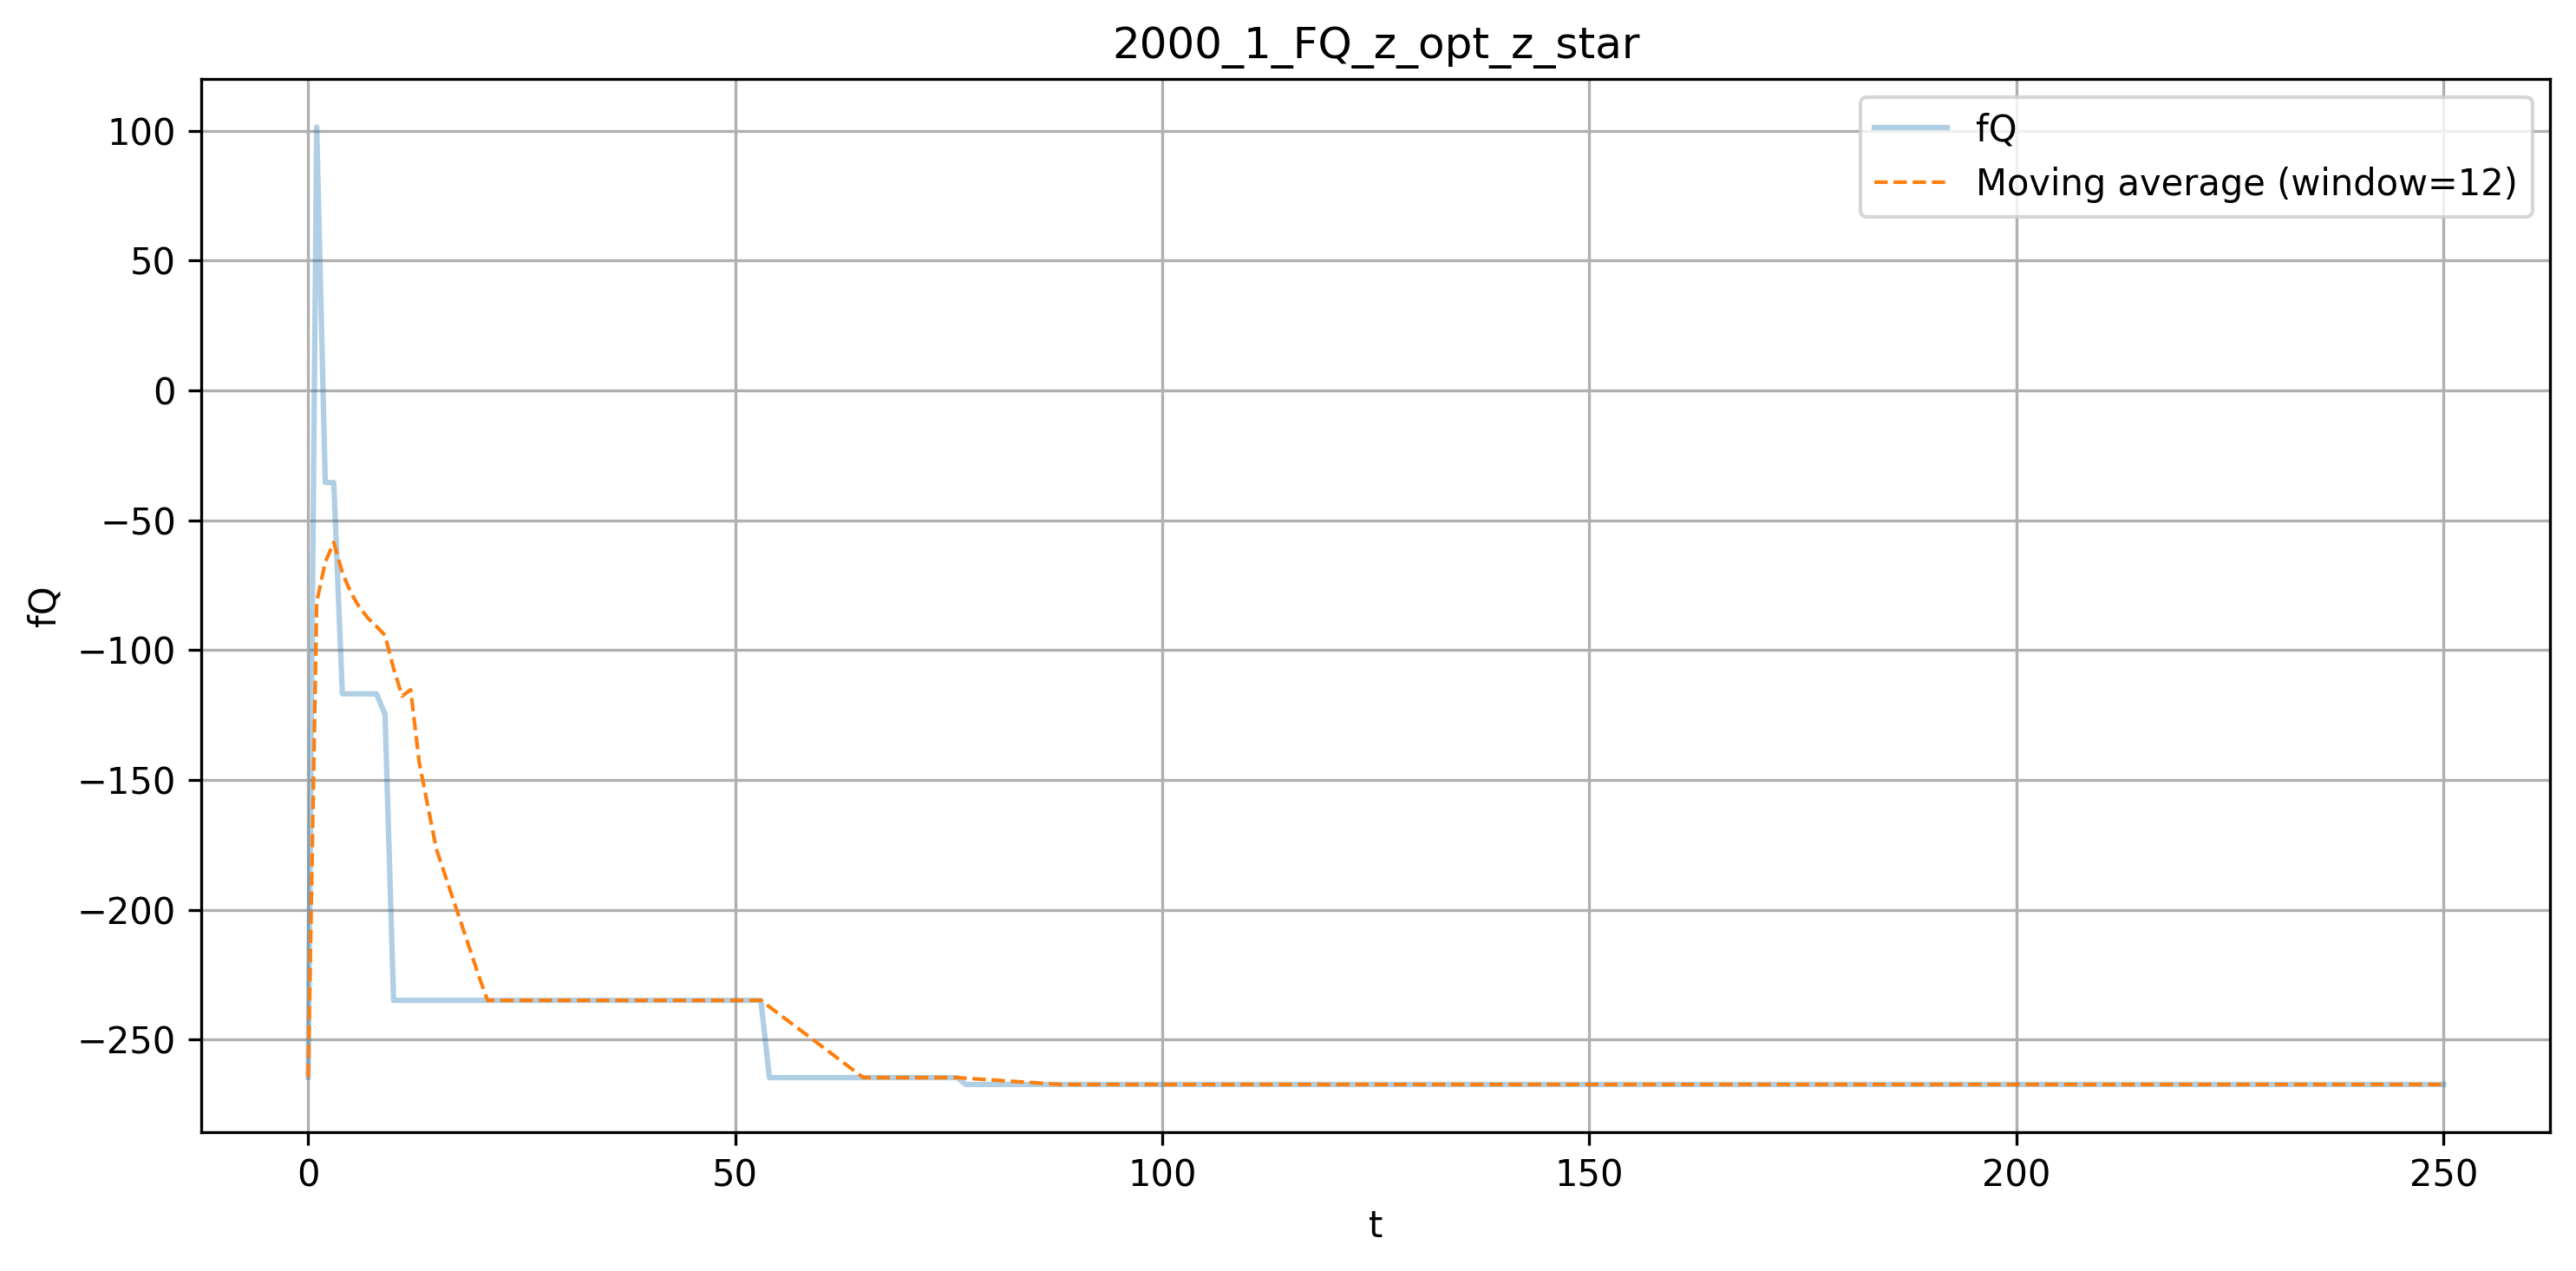
\includegraphics[width=\linewidth]{../Quantum-Annealing-for-solving-QUBO-Problems/test/Diagnostica_QALS/2/Decay_factor/ksp_1/lambda_650_dot_C/2000_1_FQ_z_opt_z_star.png}
    \caption{\(f_Q(z_\star)\) con \(\lambda_1\)}
    \label{fig:fQ-zstar-lambda1}
\end{subfigure}
\hfill
\begin{subfigure}{0.495\textwidth}
    \centering
    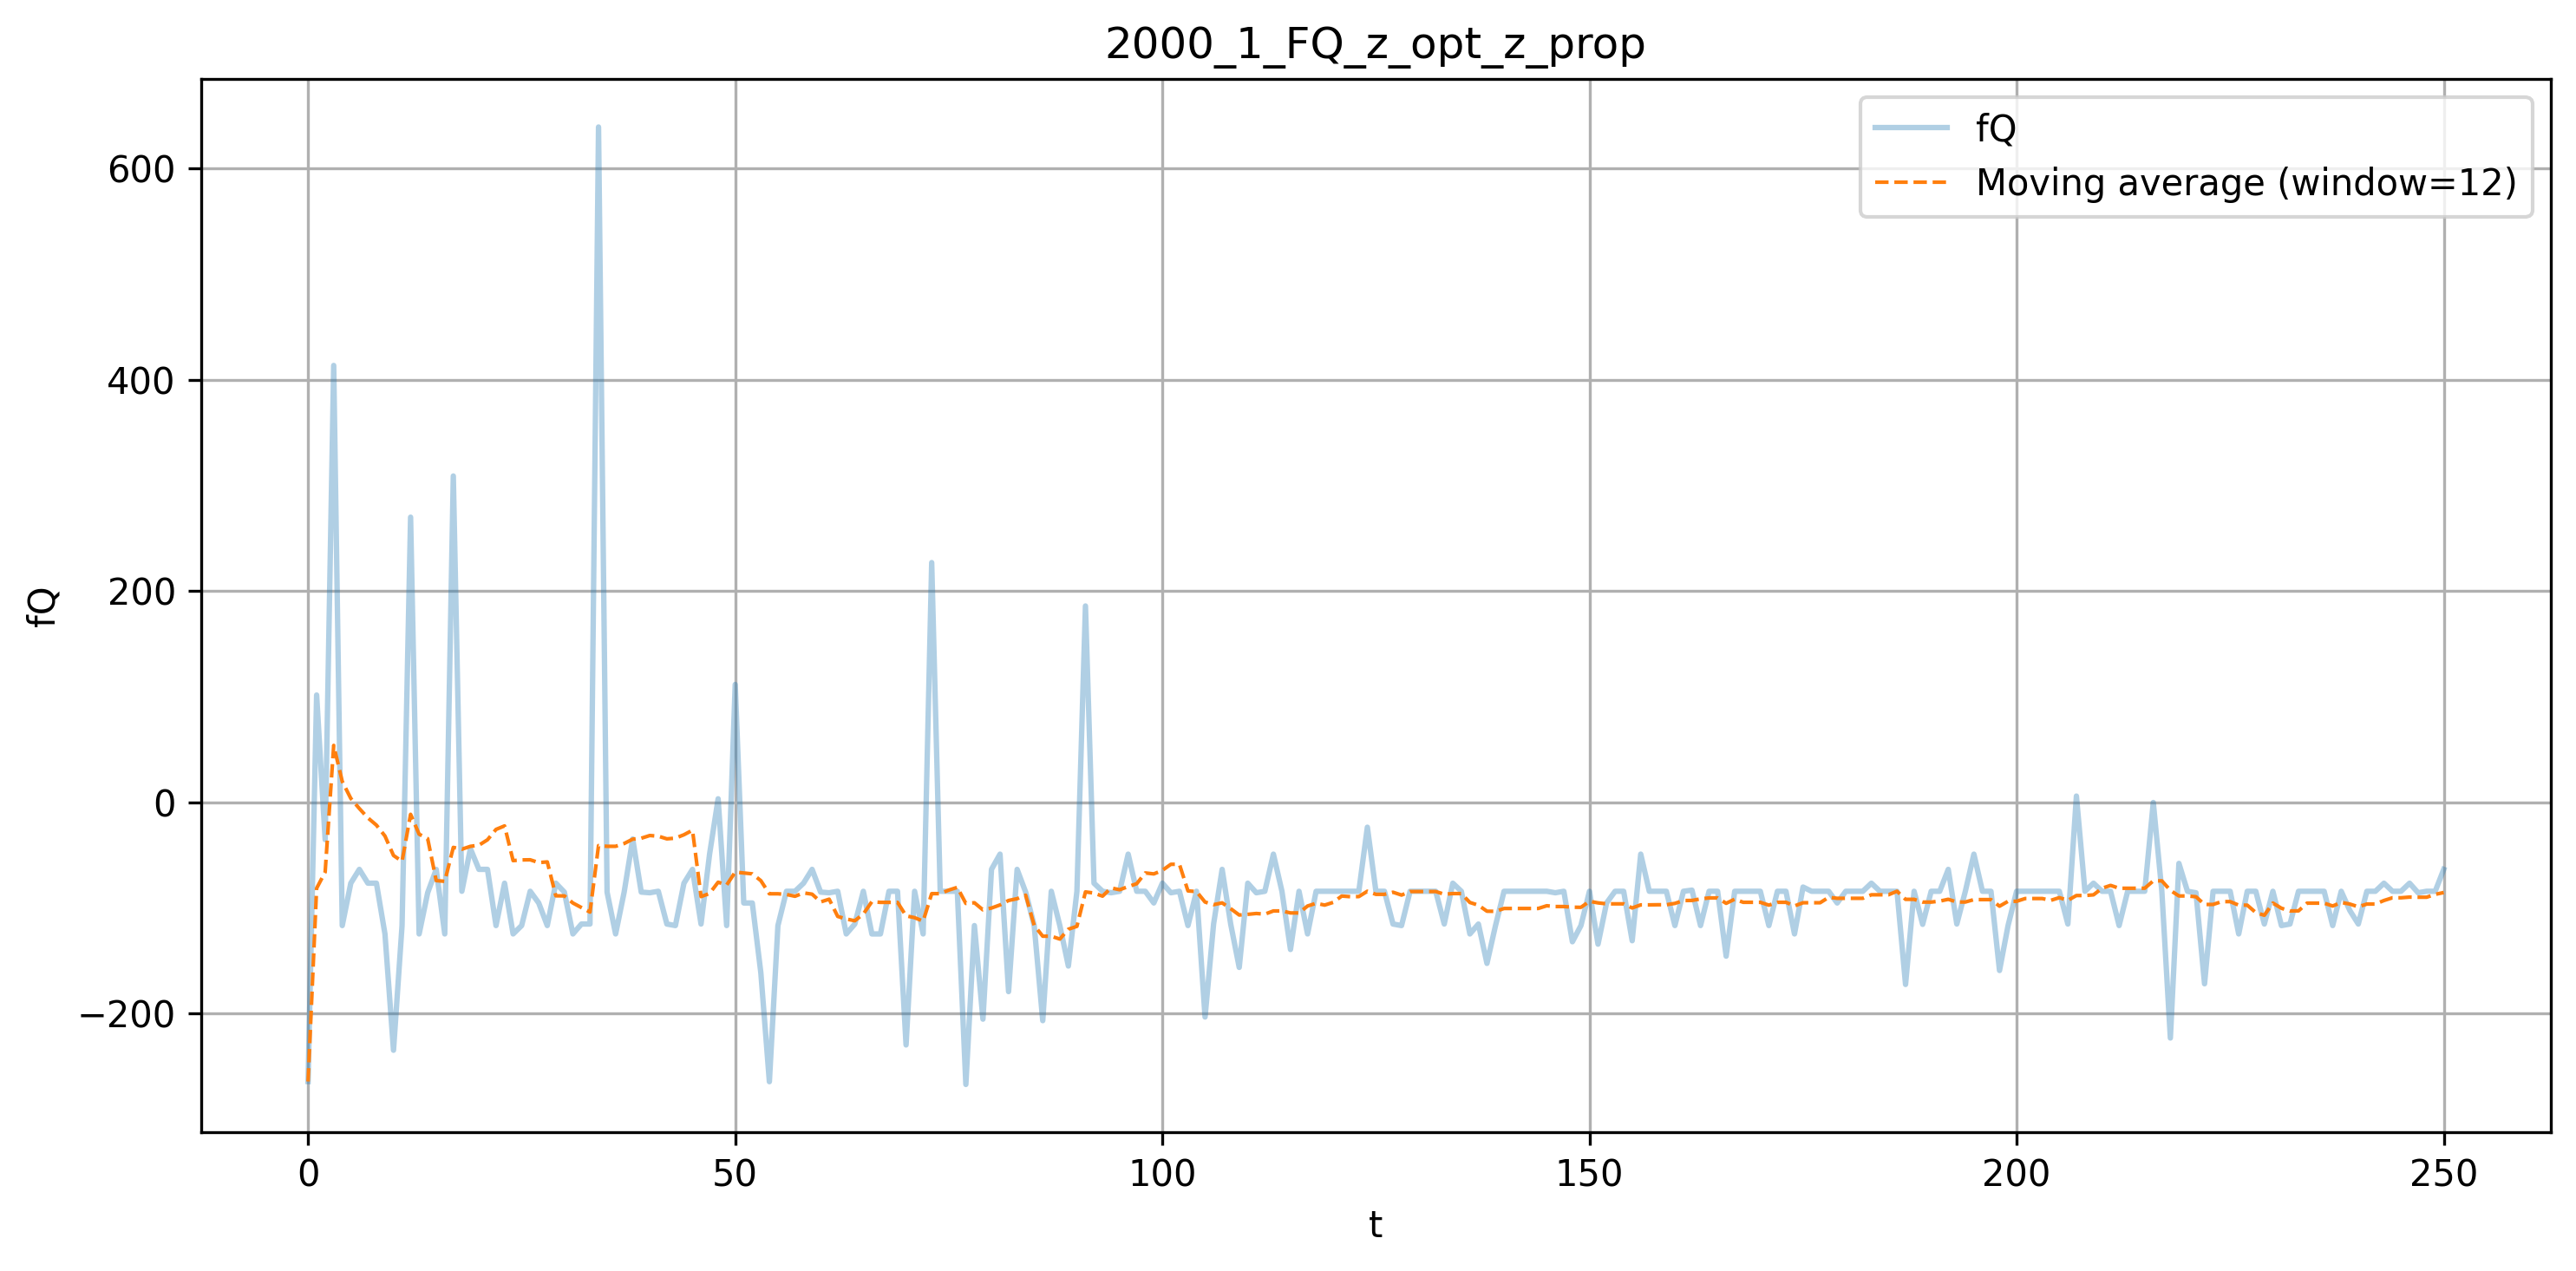
\includegraphics[width=\linewidth]{../Quantum-Annealing-for-solving-QUBO-Problems/test/Diagnostica_QALS/2/Decay_factor/ksp_1/lambda_650_dot_C/2000_1_FQ_z_opt_z_prop.png}
    \caption{\(f_Q(z_t)\) con \(\lambda_1\)}
    \label{fig:fQ-zt-lambda1}
\end{subfigure}
\label{fig:confronto-hamming-ksp11}
\end{figure}

\begin{figure}[H]
\centering
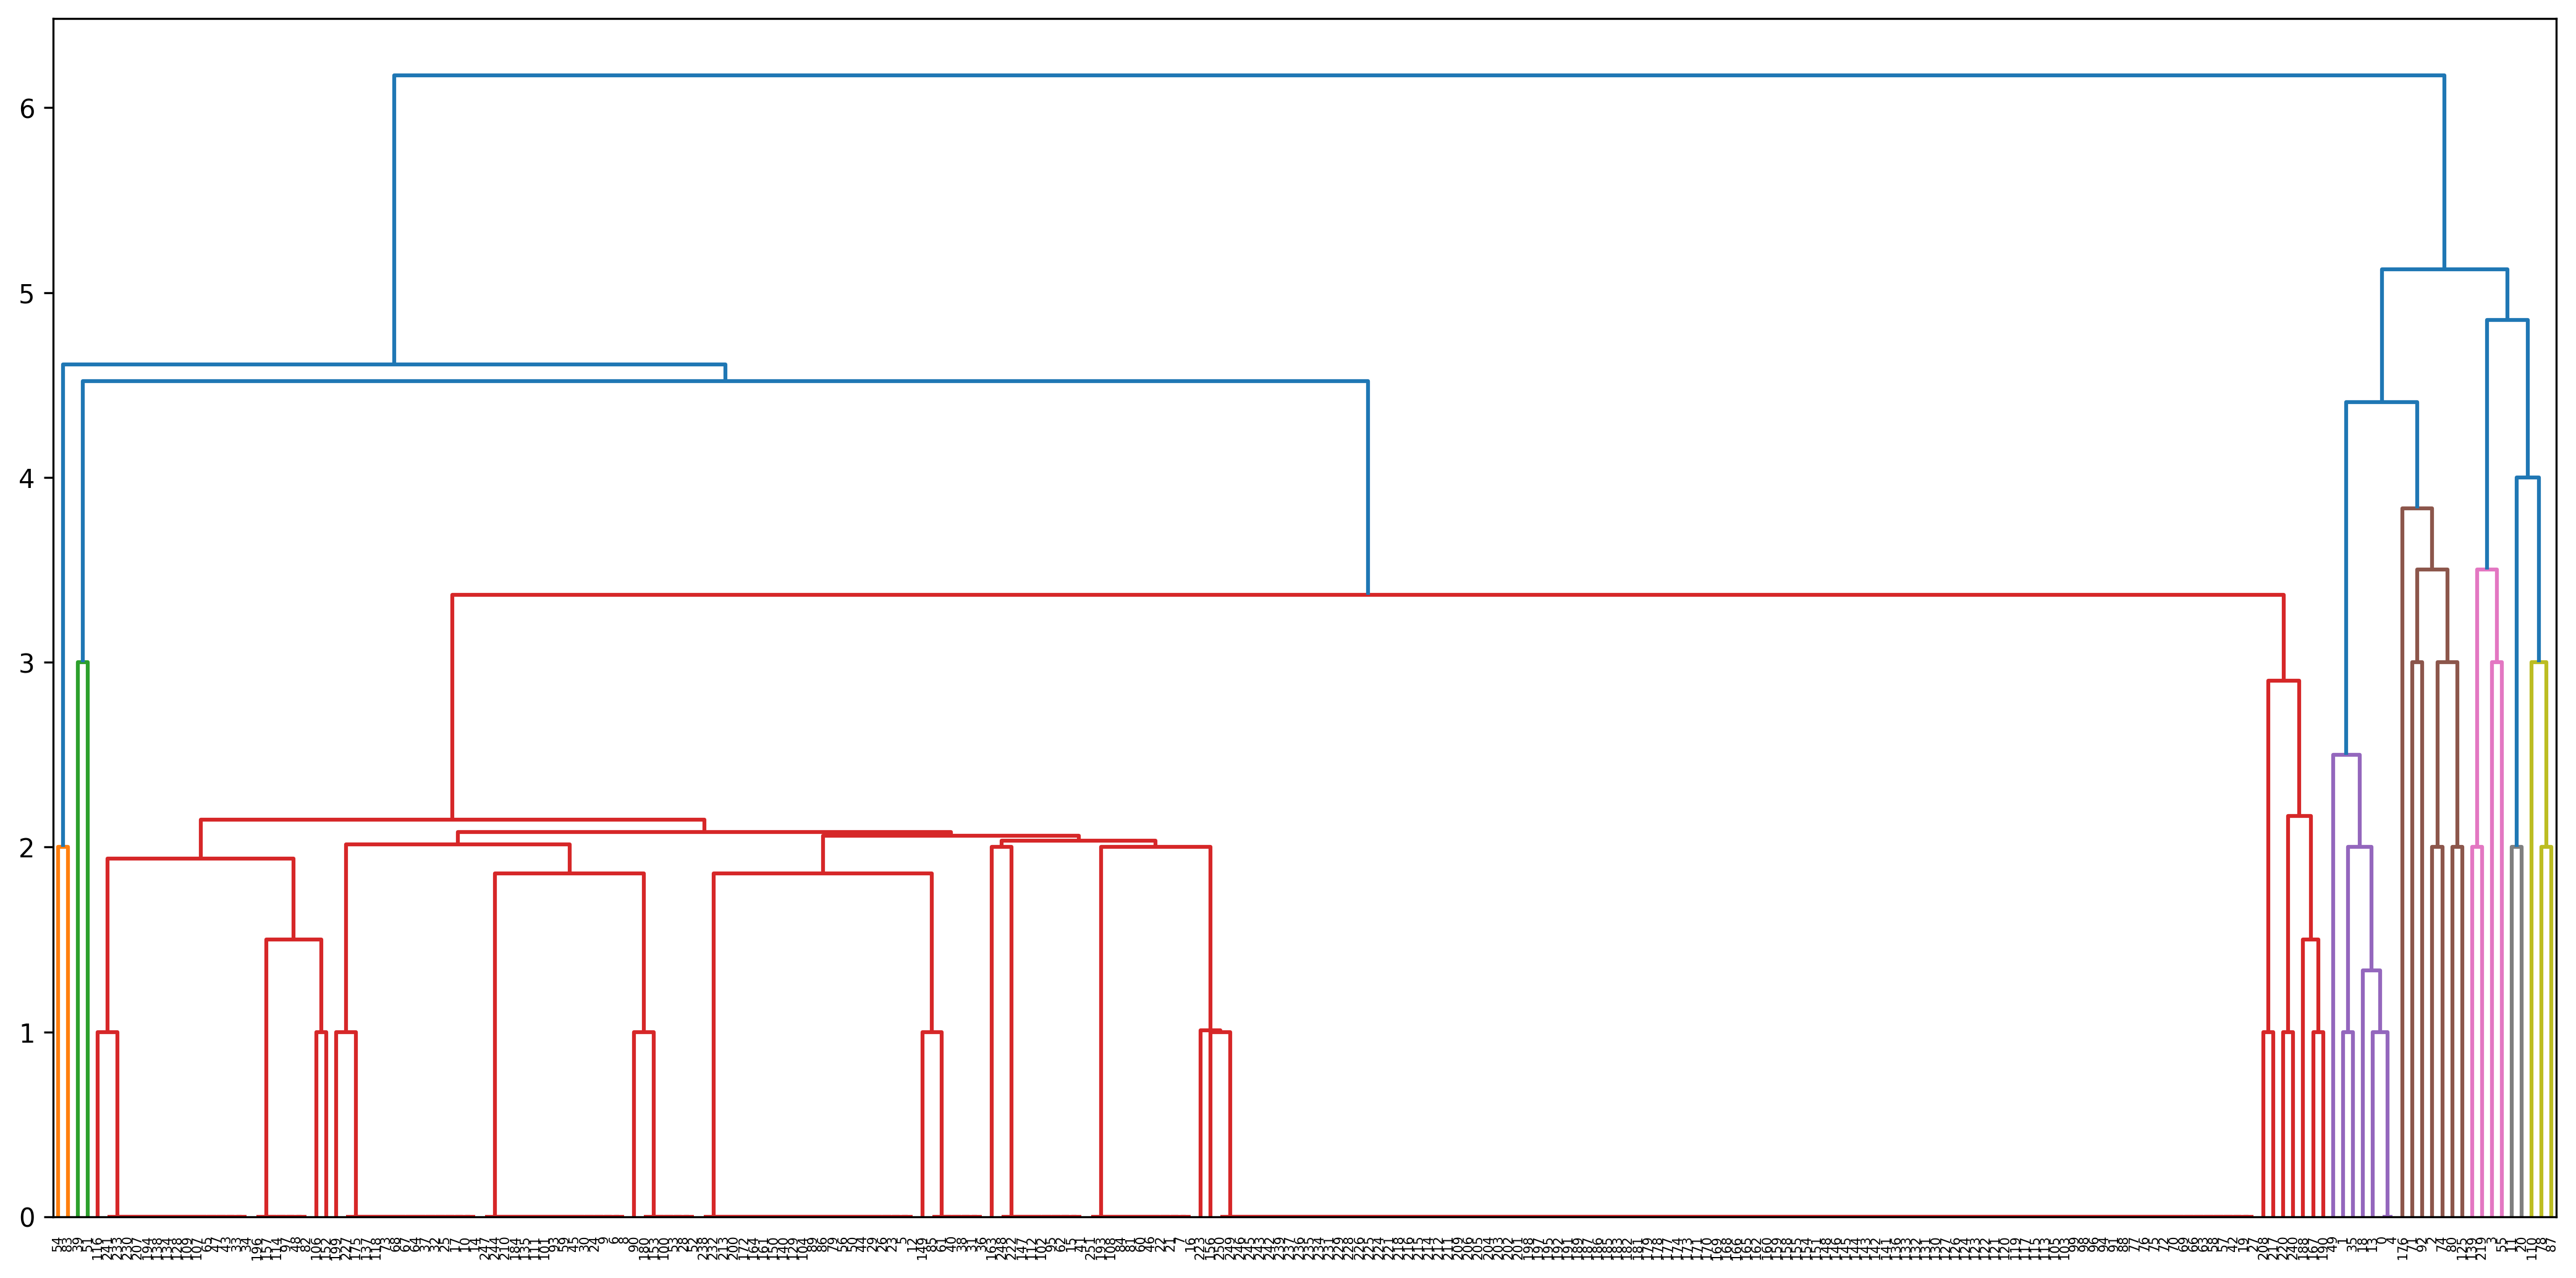
\includegraphics[width=\linewidth]{../Quantum-Annealing-for-solving-QUBO-Problems/test/Diagnostica_QALS/2/Decay_factor/ksp_1/lambda_650_dot_C/dendrogram_2000_1.png}
\caption{Agglomerative Clustering Dendogram}
\label{fig:AgglomerativeClustering-ksp1}
\end{figure}

\clearpage
\begin{figure}[H]
\centering
\begin{subfigure}{0.495\textwidth}
    \centering
    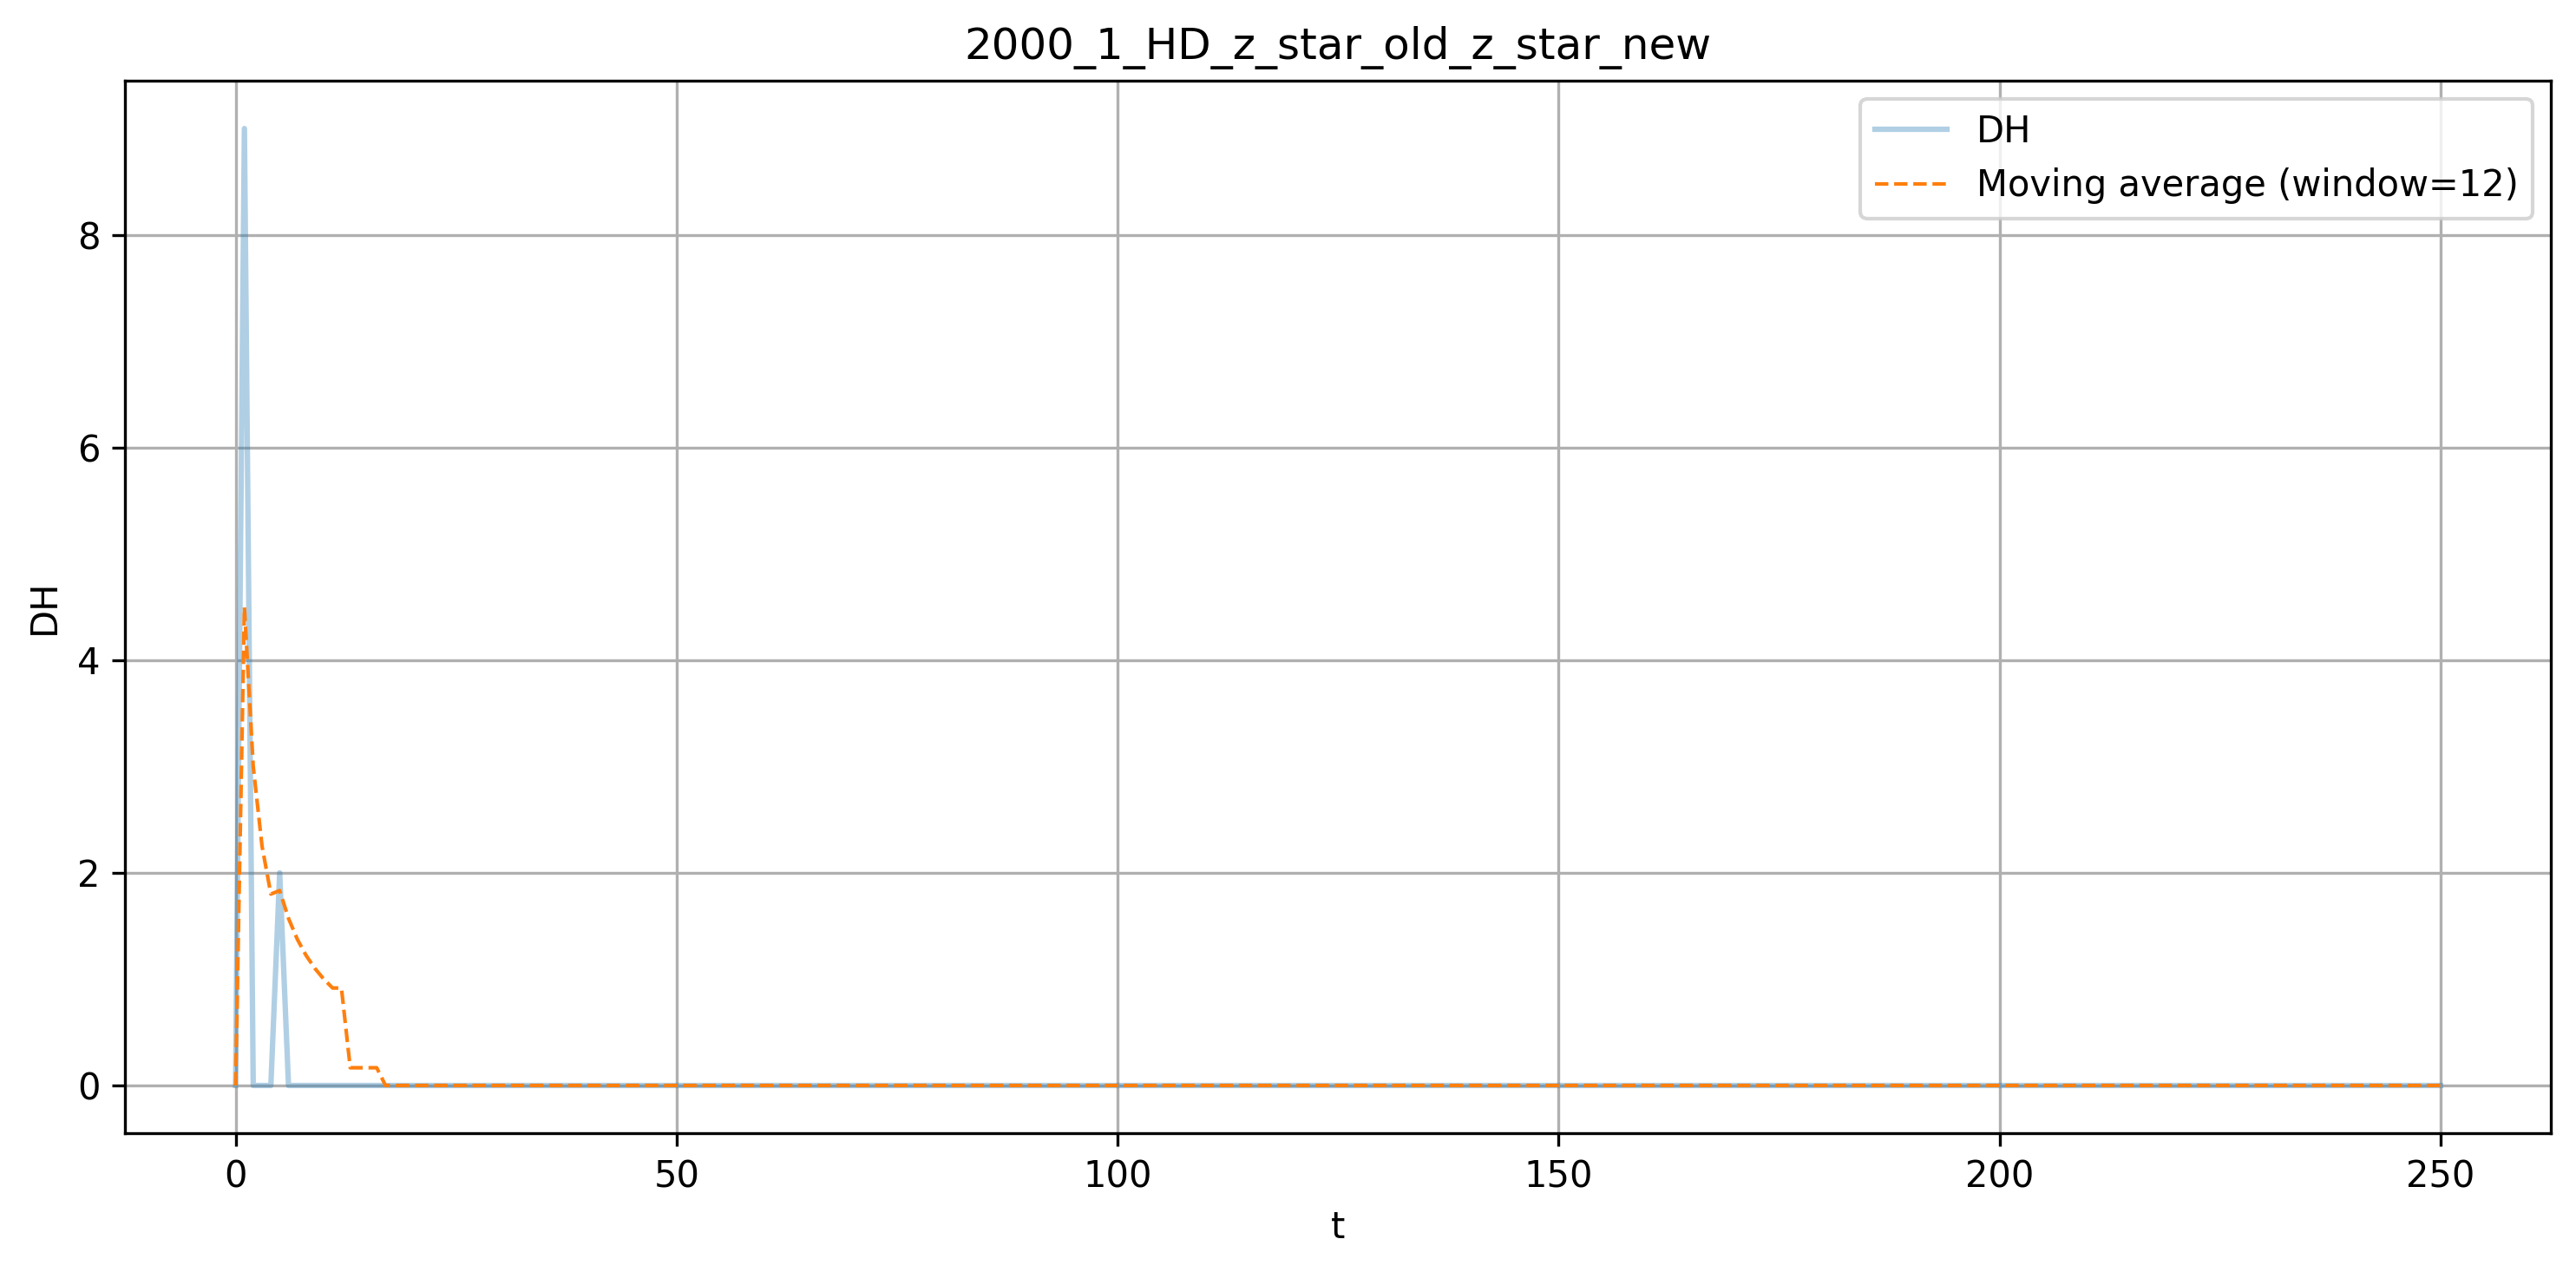
\includegraphics[width=\linewidth]{../Quantum-Annealing-for-solving-QUBO-Problems/test/Diagnostica_QALS/2/Decay_factor/ksp_1/lambda_div_3/2000_1_HD_z_star_old_z_star_new.png}
    \caption{\(d_H(z_\star^{old}, z_\star^{new})\) con \(\lambda_2\)}
    \label{fig:hd-zstarold-zstarnew-lambda2}
\end{subfigure}
\hfill
\begin{subfigure}{0.495\textwidth}
    \centering
    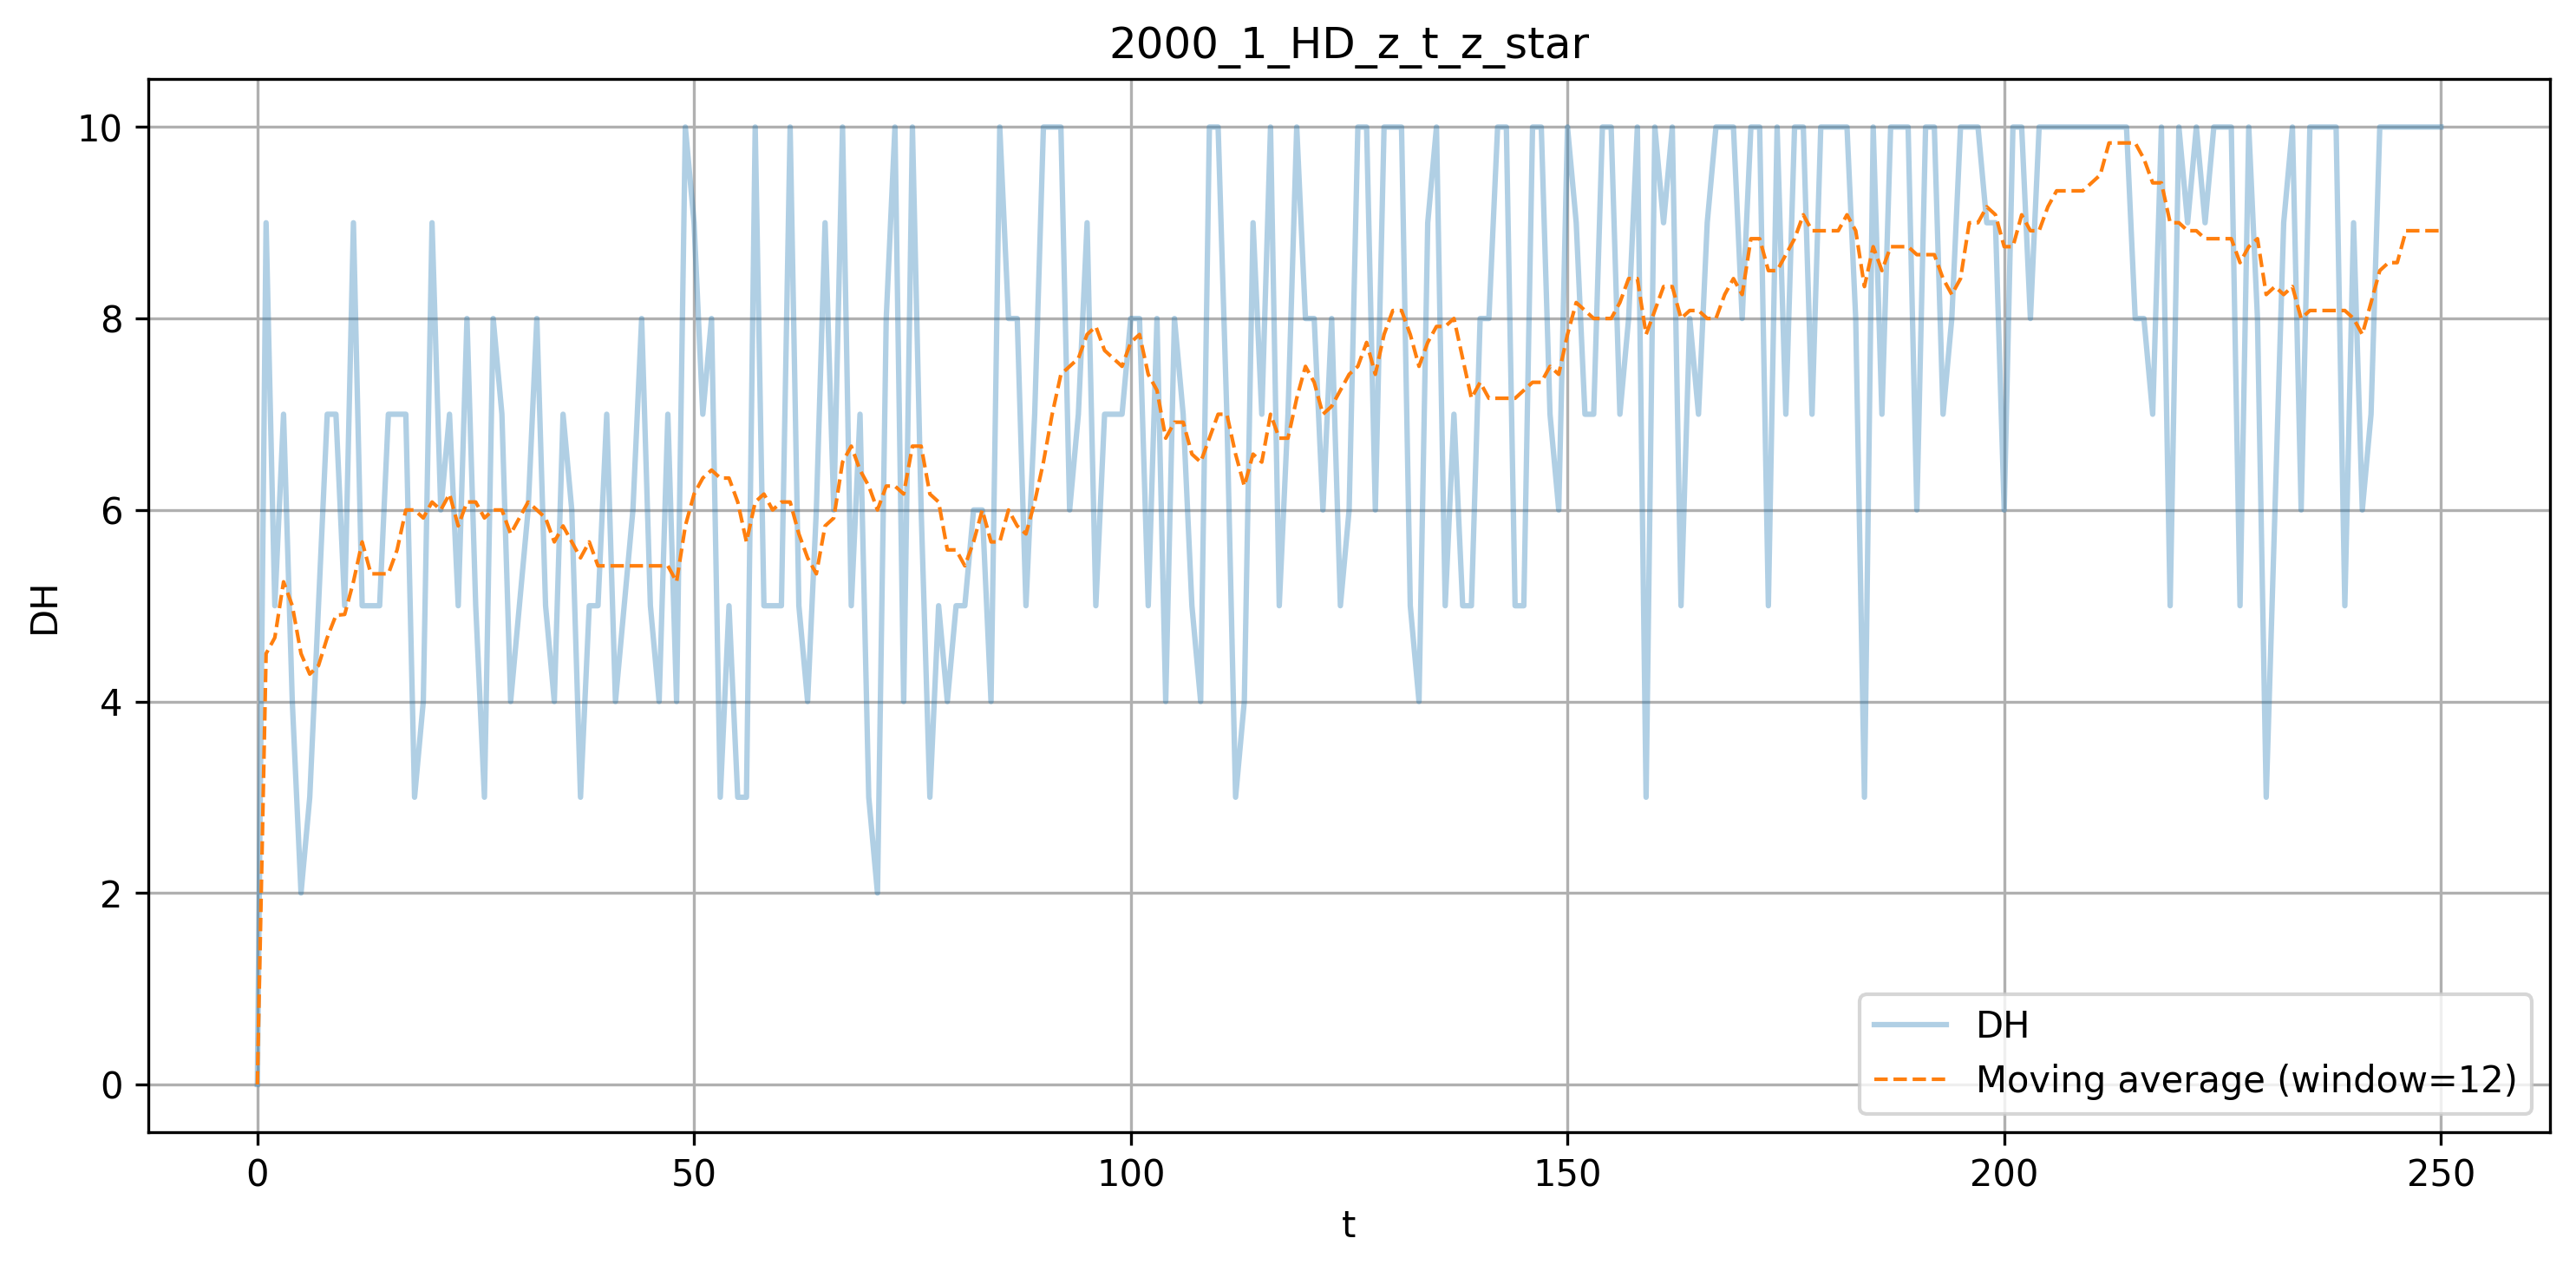
\includegraphics[width=\linewidth]{../Quantum-Annealing-for-solving-QUBO-Problems/test/Diagnostica_QALS/2/Decay_factor/ksp_1/lambda_div_3/2000_1_HD_z_t_z_star.png}
    \caption{\(d_H(z_t, z_\star)\) con \(\lambda_2\)}
    \label{fig:hd-zt-zstar-lambda2}
\end{subfigure}

\vspace{0.35cm}

\begin{subfigure}{0.495\textwidth}
    \centering
    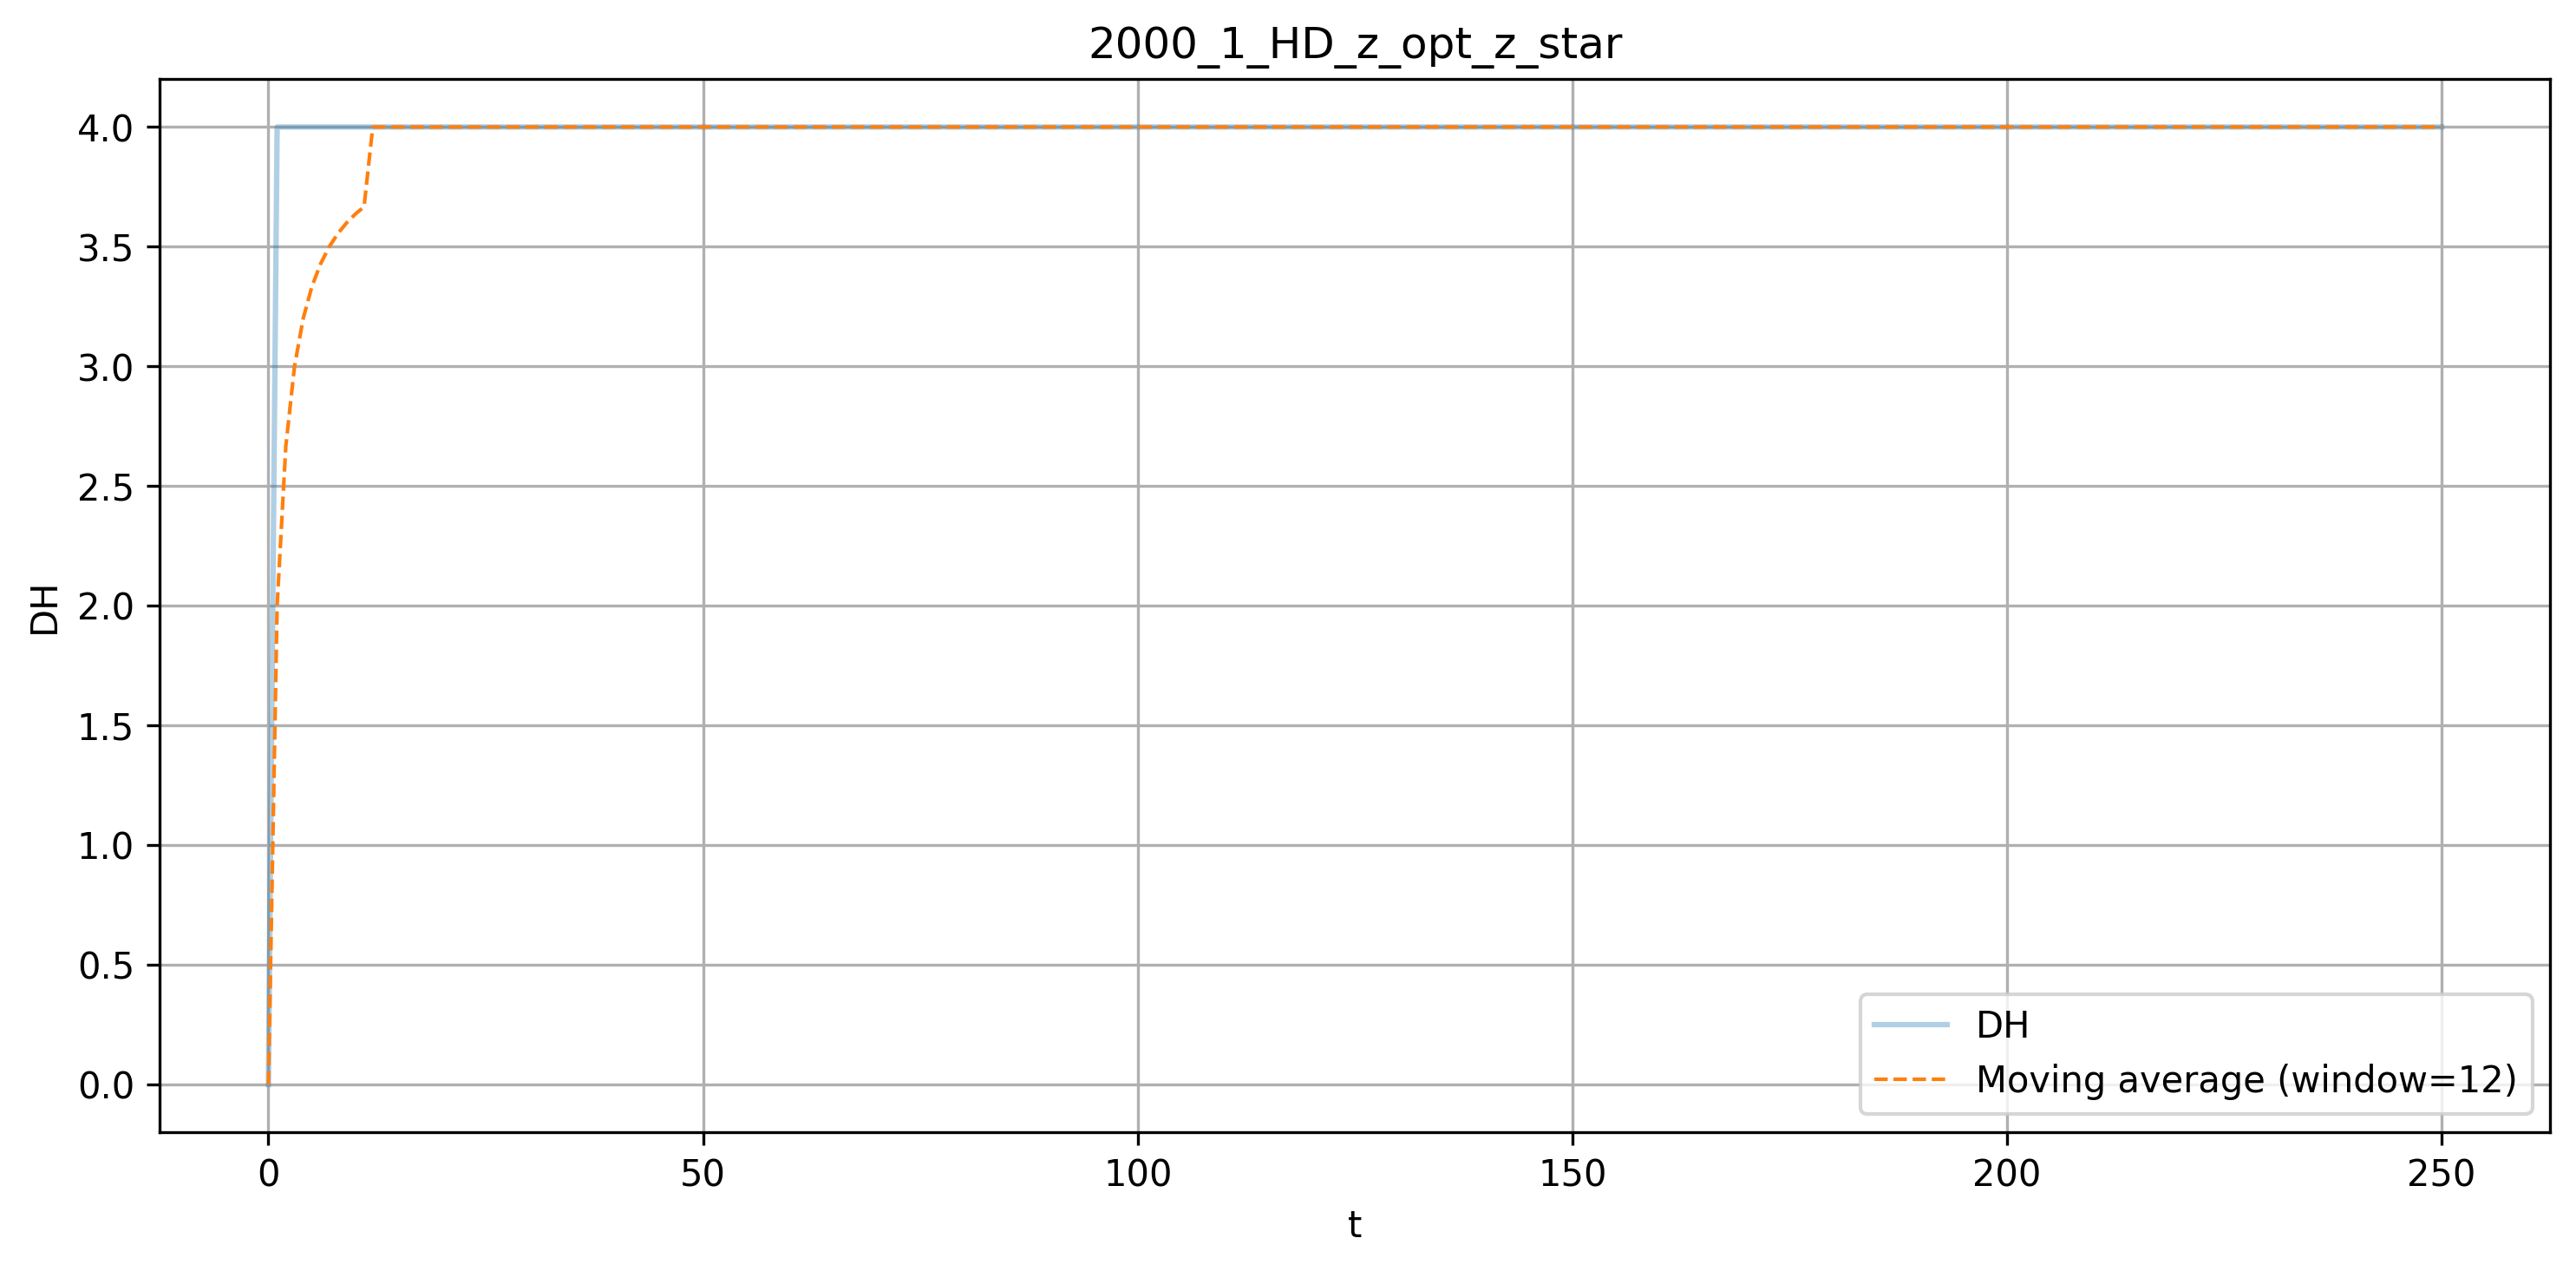
\includegraphics[width=\linewidth]{../Quantum-Annealing-for-solving-QUBO-Problems/test/Diagnostica_QALS/2/Decay_factor/ksp_1/lambda_div_3/2000_1_HD_z_opt_z_star.png}
    \caption{\(d_H(z_{opt}, z_\star)\) con \(\lambda_2\)}
    \label{fig:hd-zopt-zstar-lambda2}
\end{subfigure}
\hfill
\begin{subfigure}{0.495\textwidth}
    \centering
    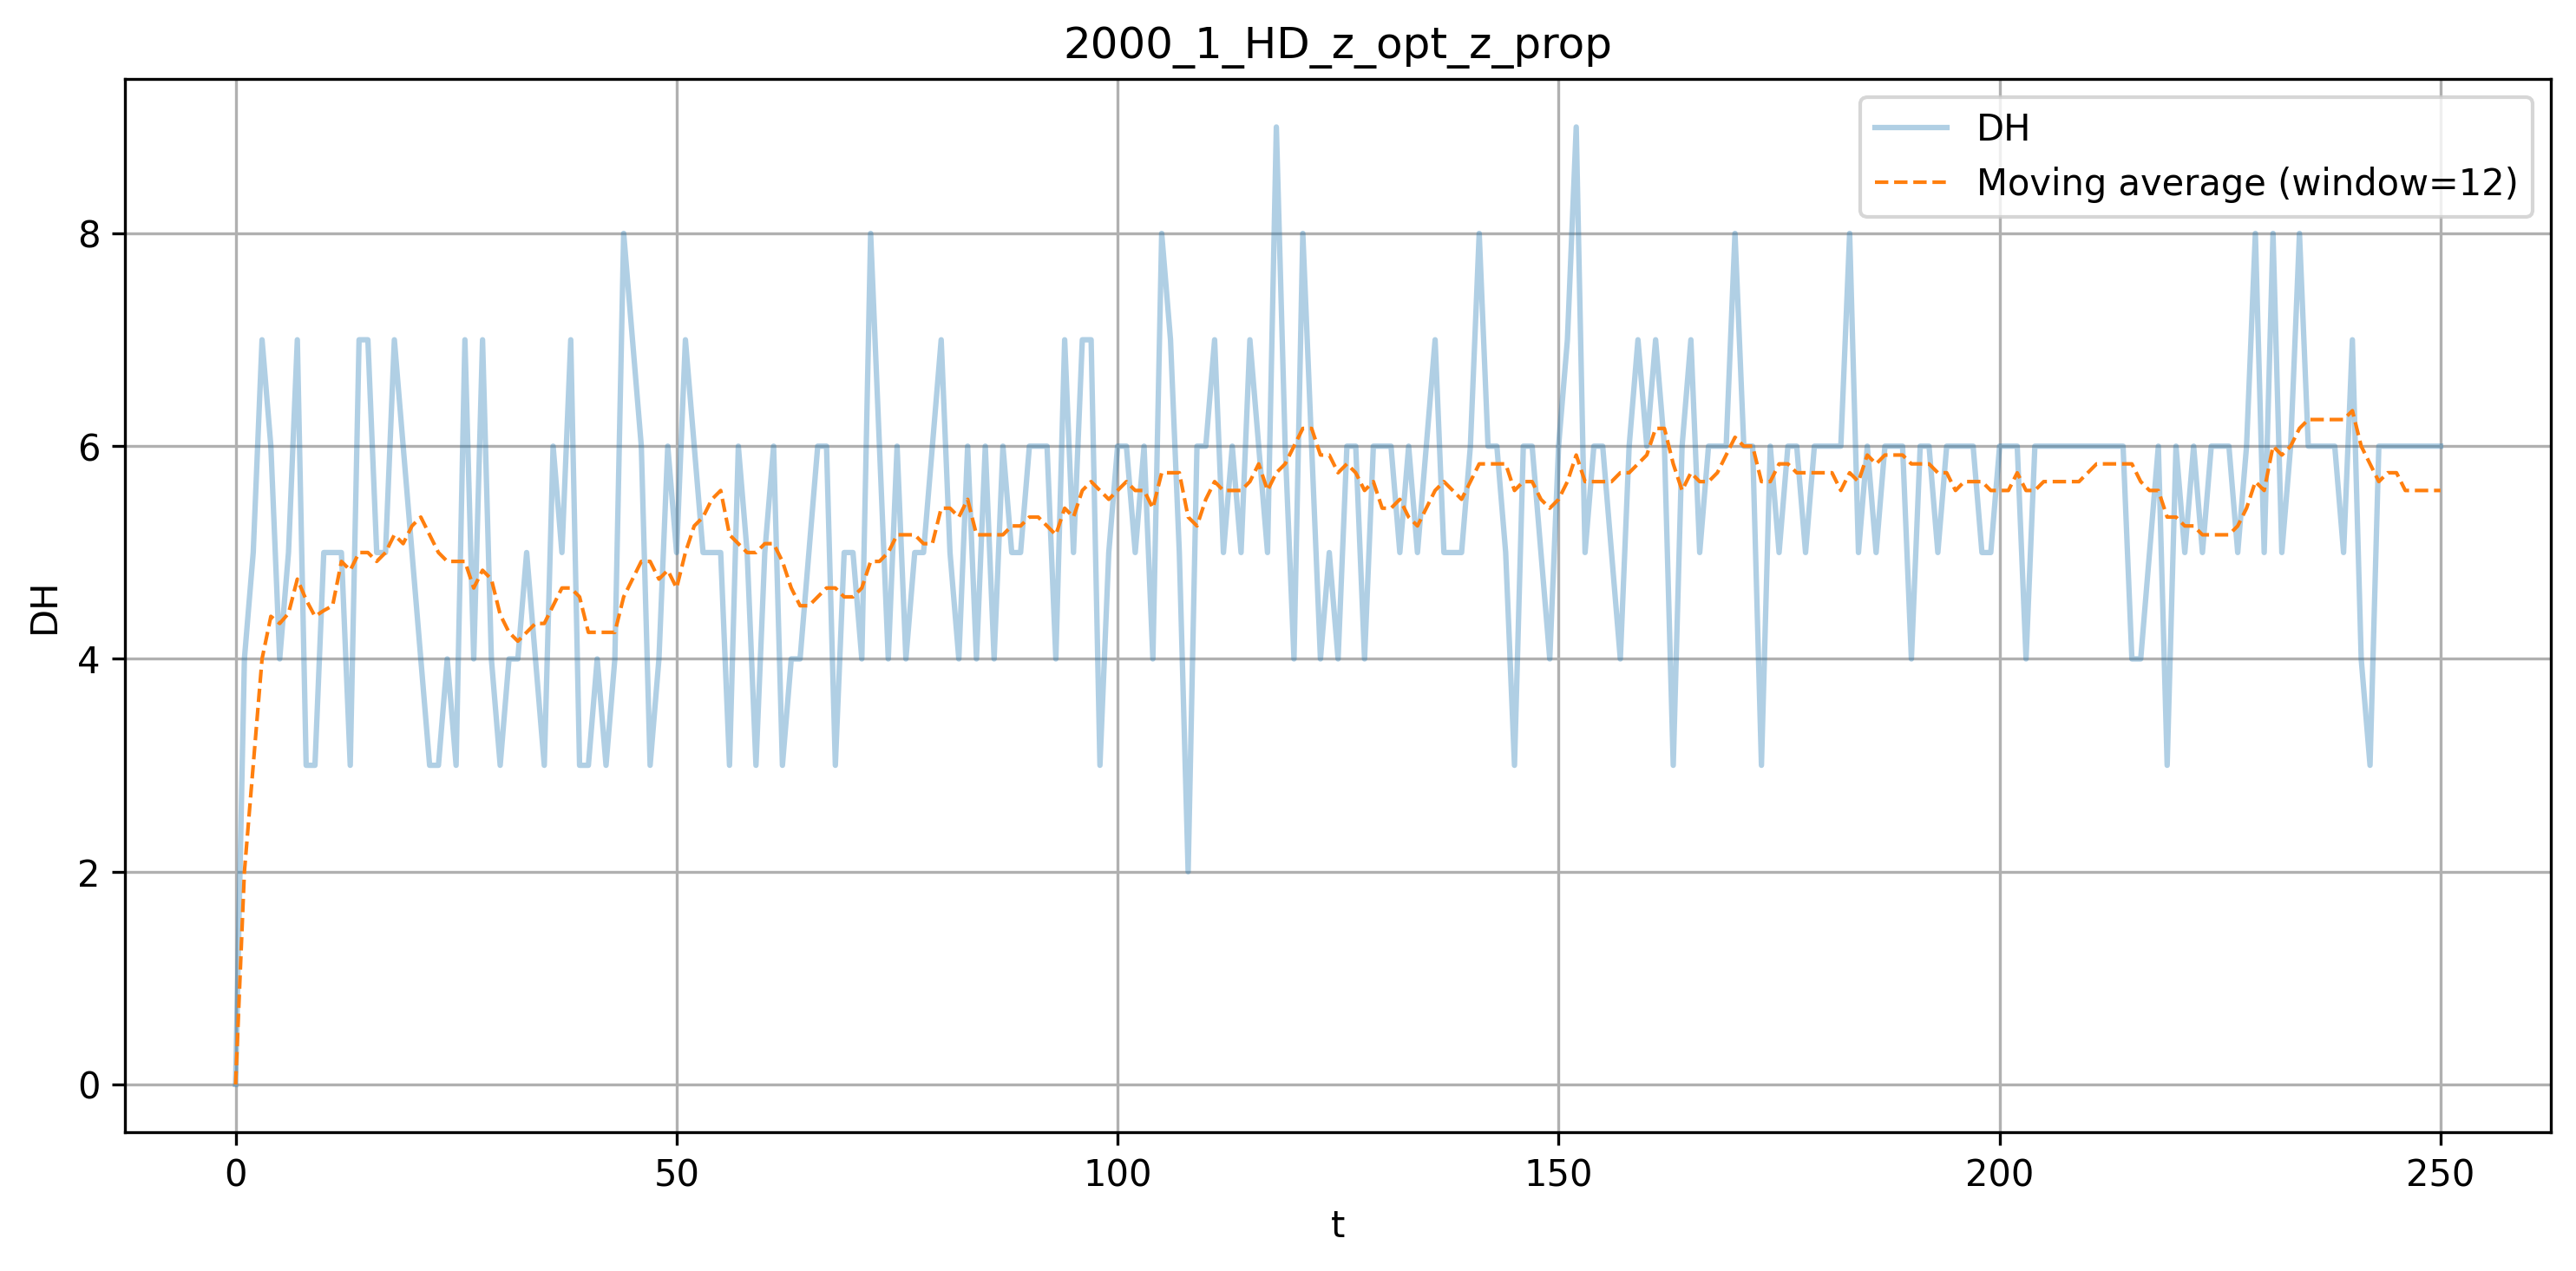
\includegraphics[width=\linewidth]{../Quantum-Annealing-for-solving-QUBO-Problems/test/Diagnostica_QALS/2/Decay_factor/ksp_1/lambda_div_3/2000_1_HD_z_opt_z_prop.png}
    \caption{\(d_H(z_{opt}, z_t)\) con \(\lambda_2\)}
    \label{fig:hd-zopt-zt-lambda2}
\end{subfigure}

\vspace{0.35cm}

\begin{subfigure}{0.495\textwidth}
    \centering
    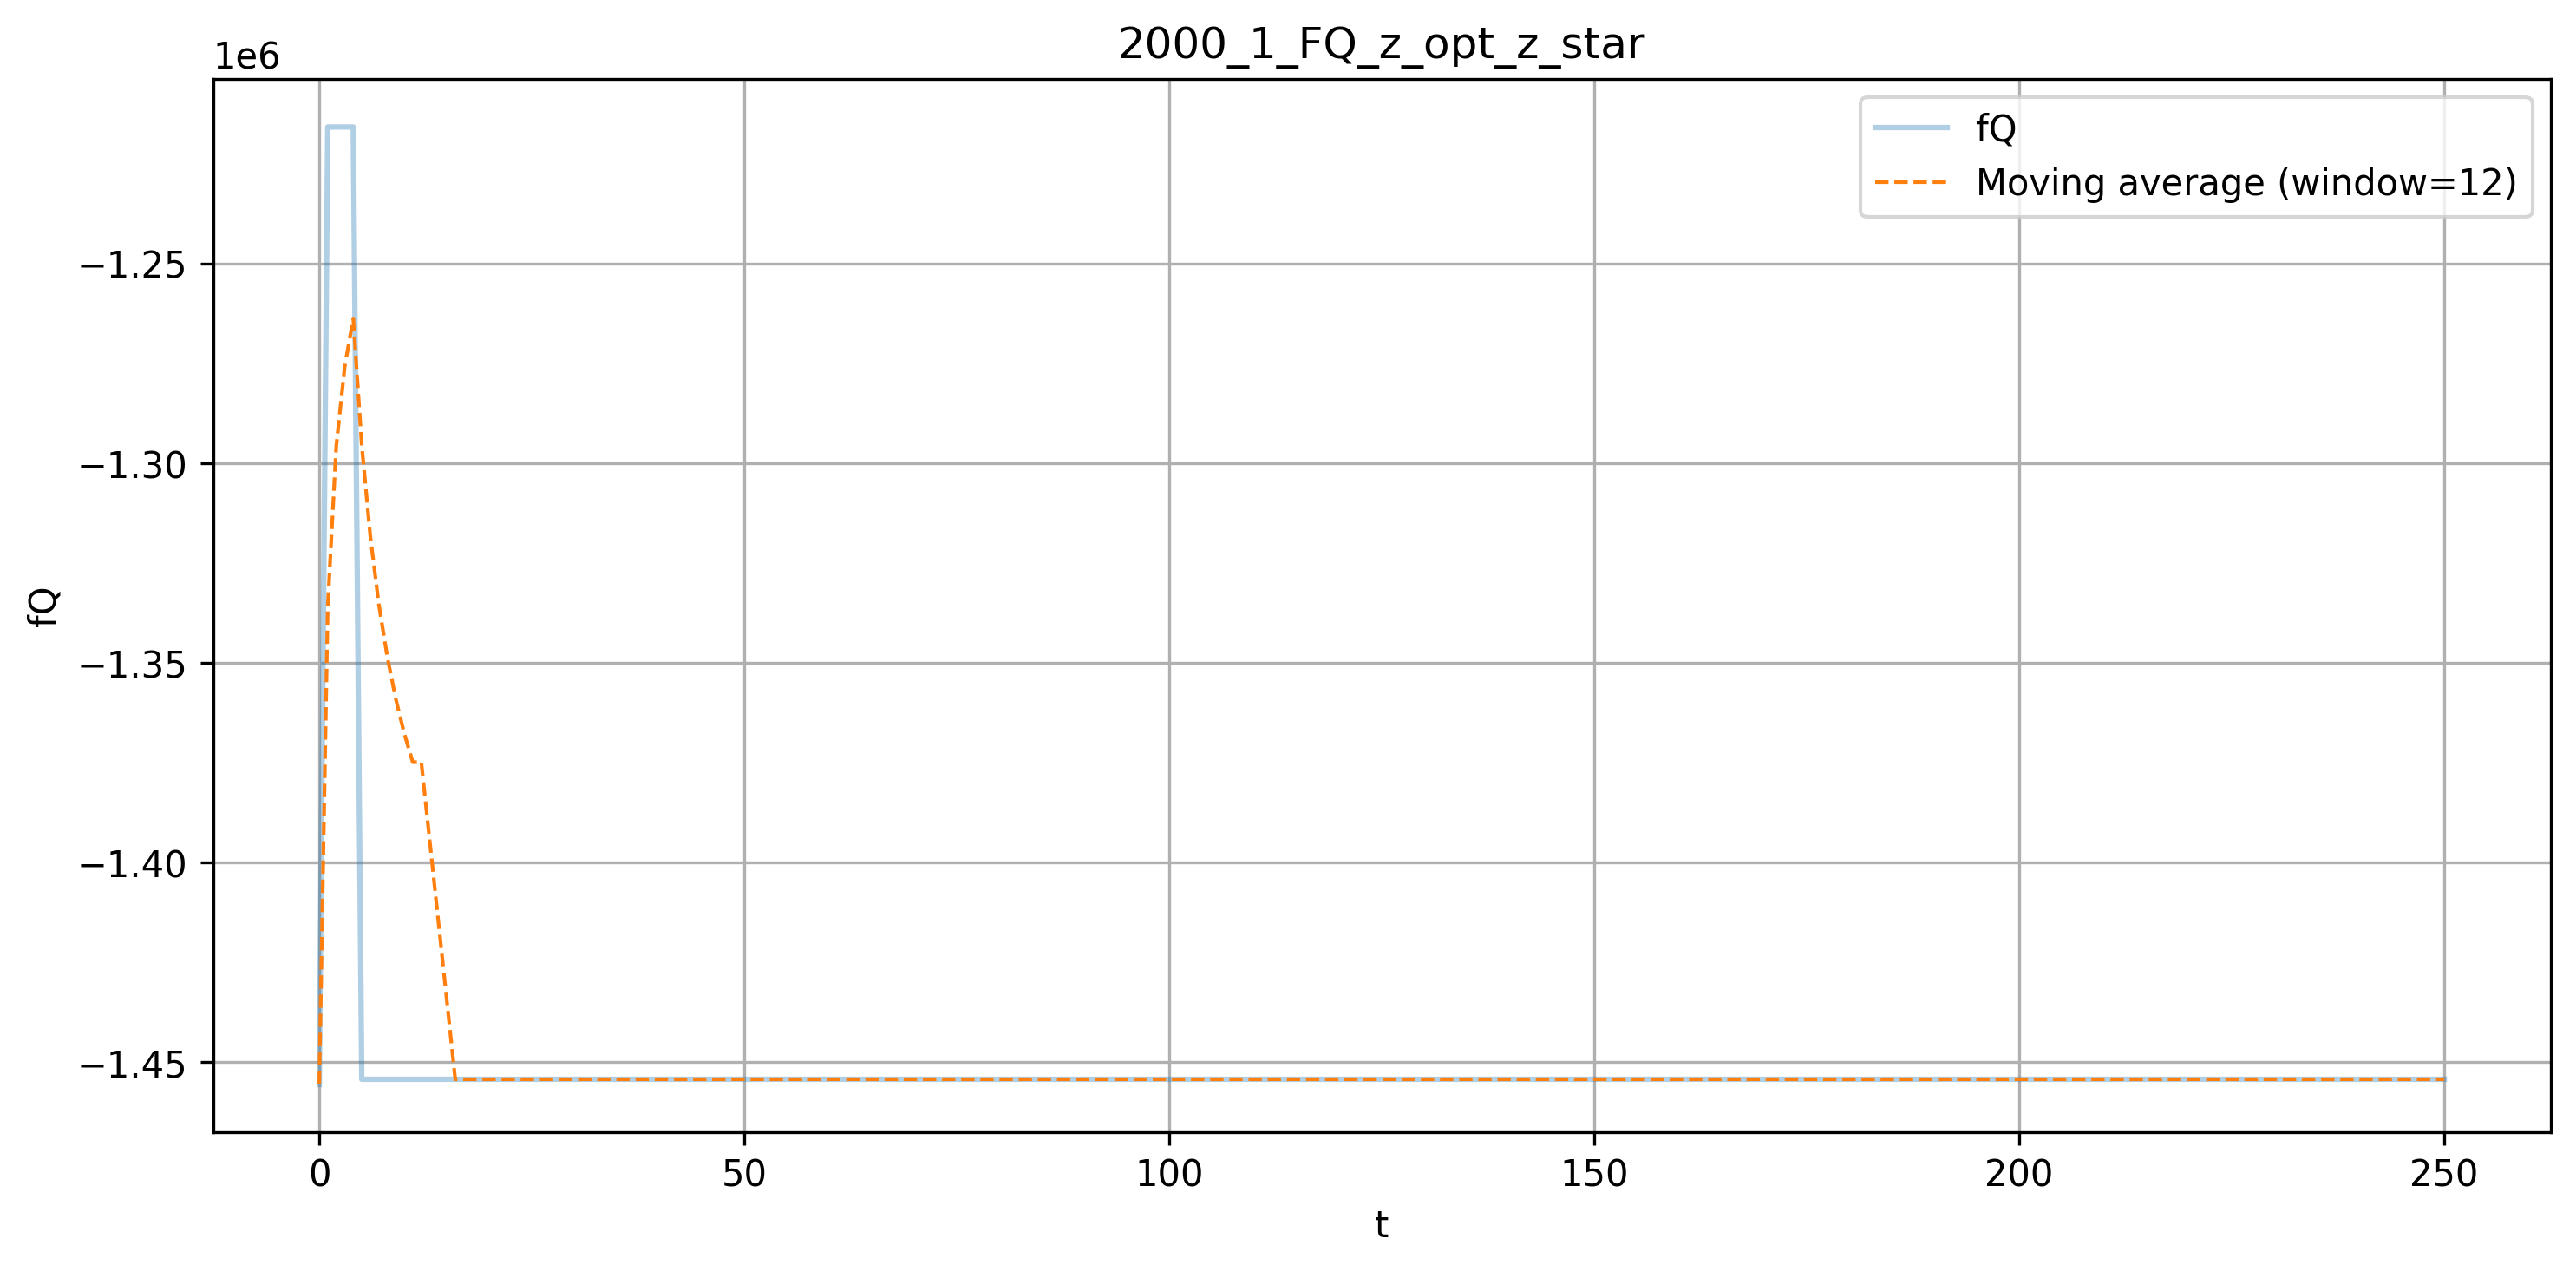
\includegraphics[width=\linewidth]{../Quantum-Annealing-for-solving-QUBO-Problems/test/Diagnostica_QALS/2/Decay_factor/ksp_1/lambda_div_3/2000_1_FQ_z_opt_z_star.png}
    \caption{\(f_Q(z_\star)\) con \(\lambda_2\)}
    \label{fig:fQ-zstar-lambda2}
\end{subfigure}
\hfill
\begin{subfigure}{0.495\textwidth}
    \centering
    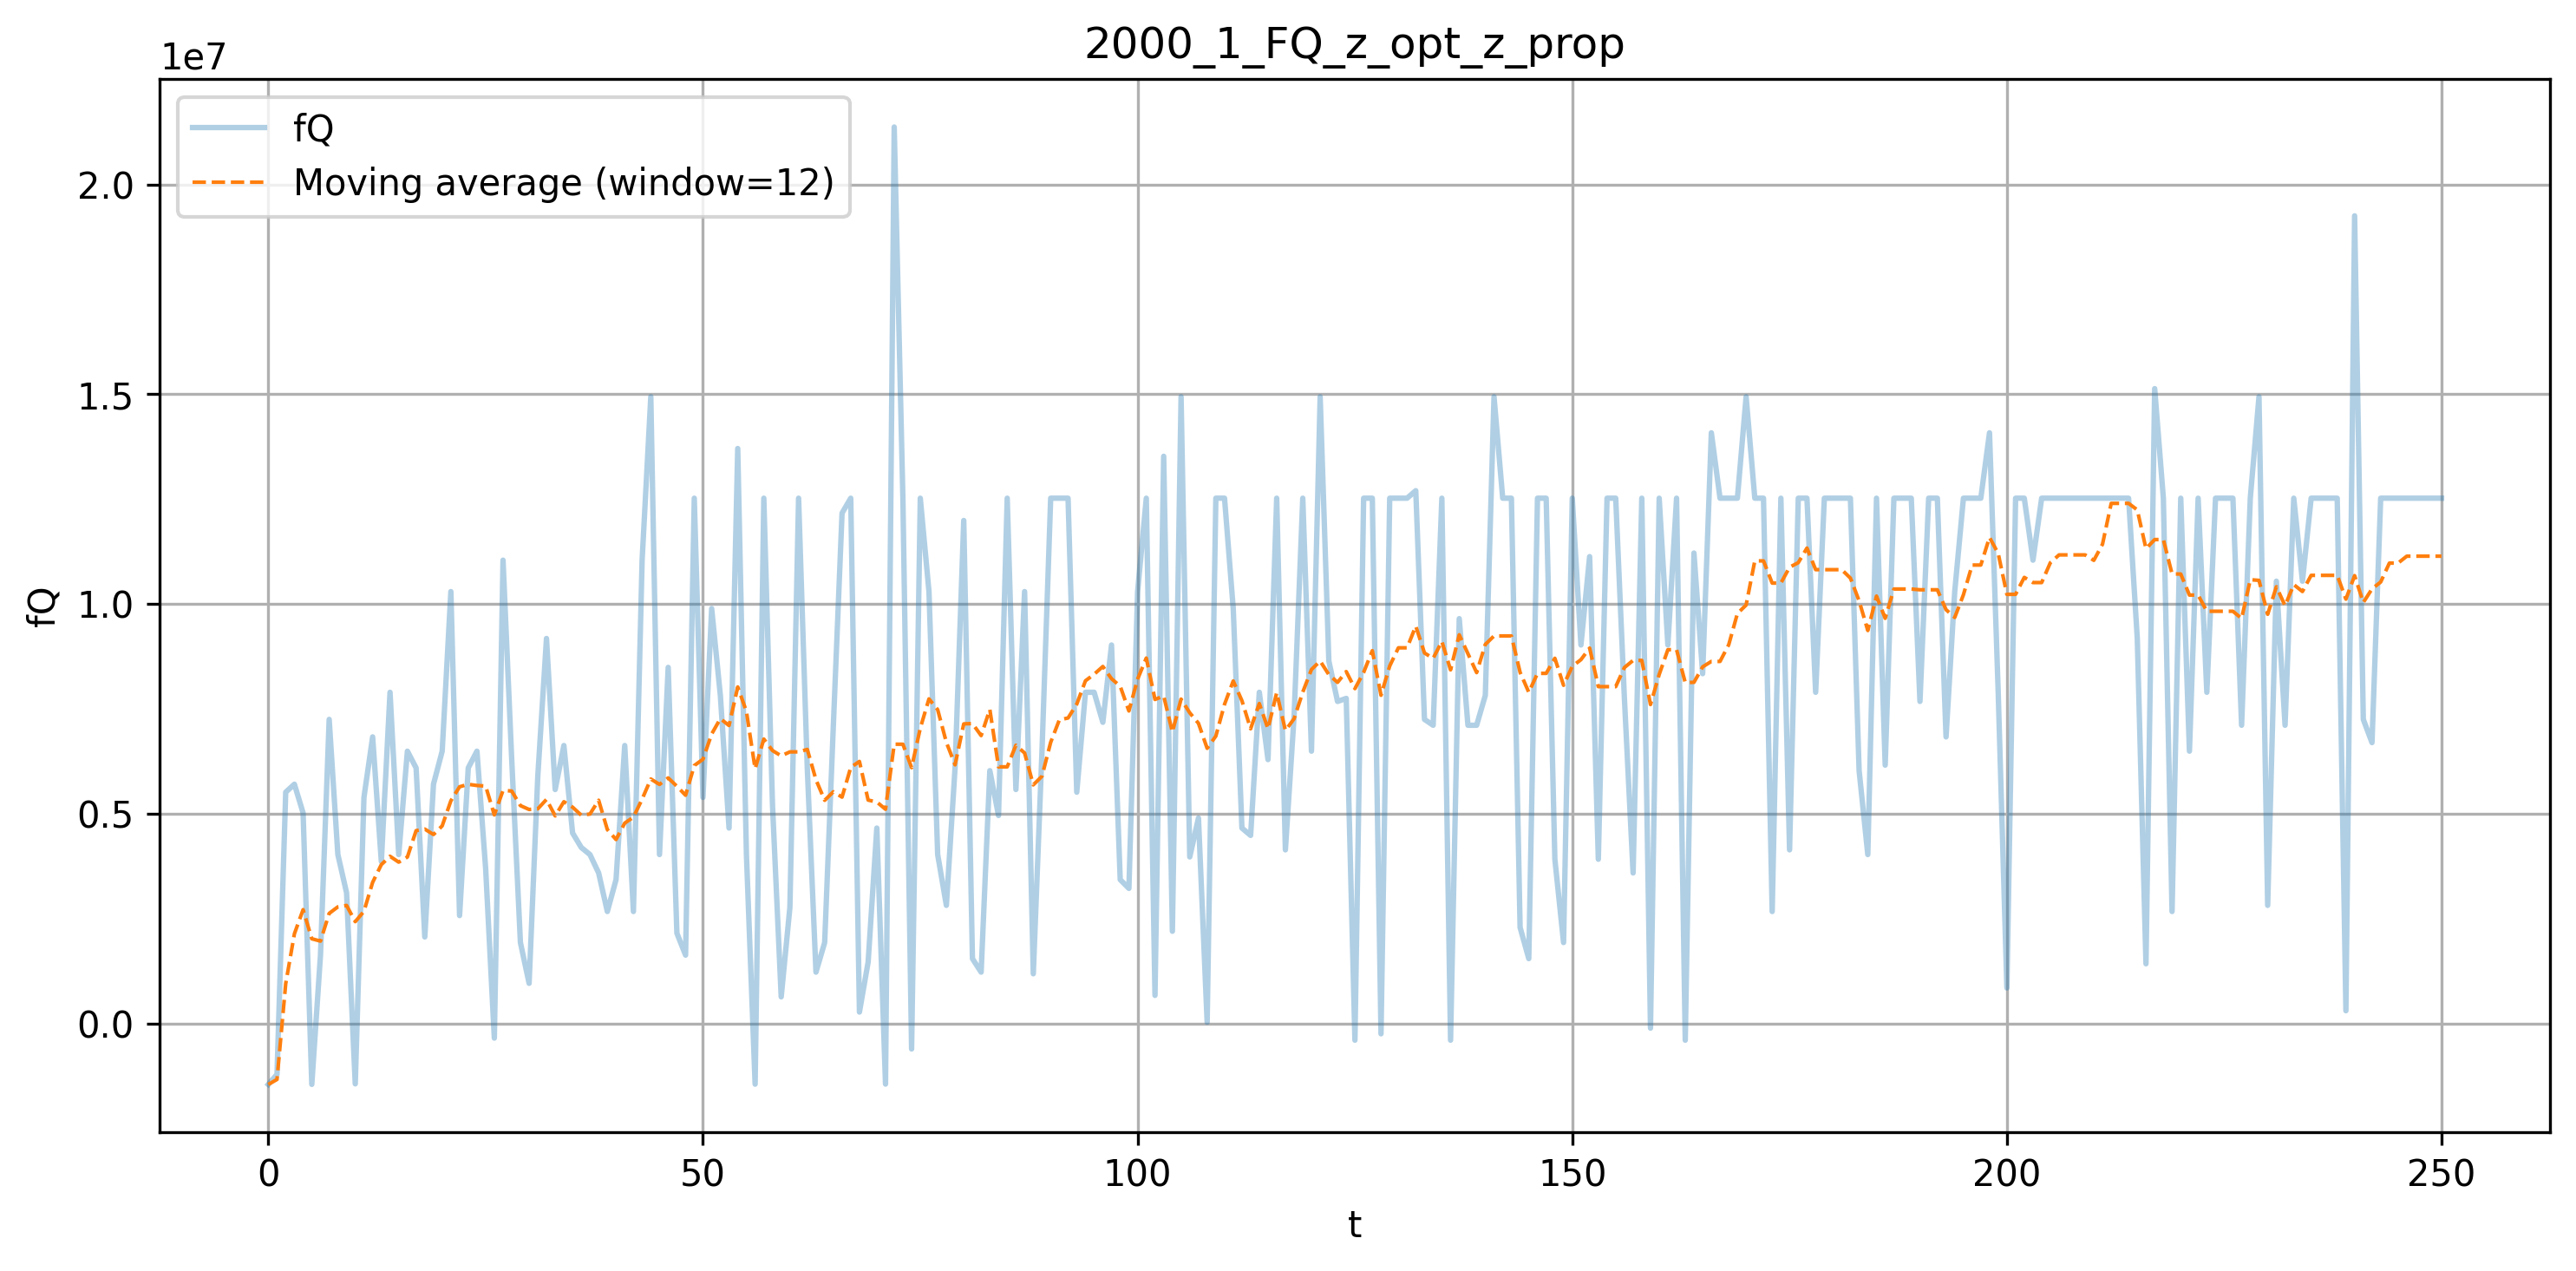
\includegraphics[width=\linewidth]{../Quantum-Annealing-for-solving-QUBO-Problems/test/Diagnostica_QALS/2/Decay_factor/ksp_1/lambda_div_3/2000_1_FQ_z_opt_z_prop.png}
    \caption{\(f_Q(z_t)\) con \(\lambda_2\)}
    \label{fig:fQ-zt-lambda2}
\end{subfigure}
\label{fig:confronto-hamming-ksp12}
\end{figure}

\begin{figure}[H]
\centering
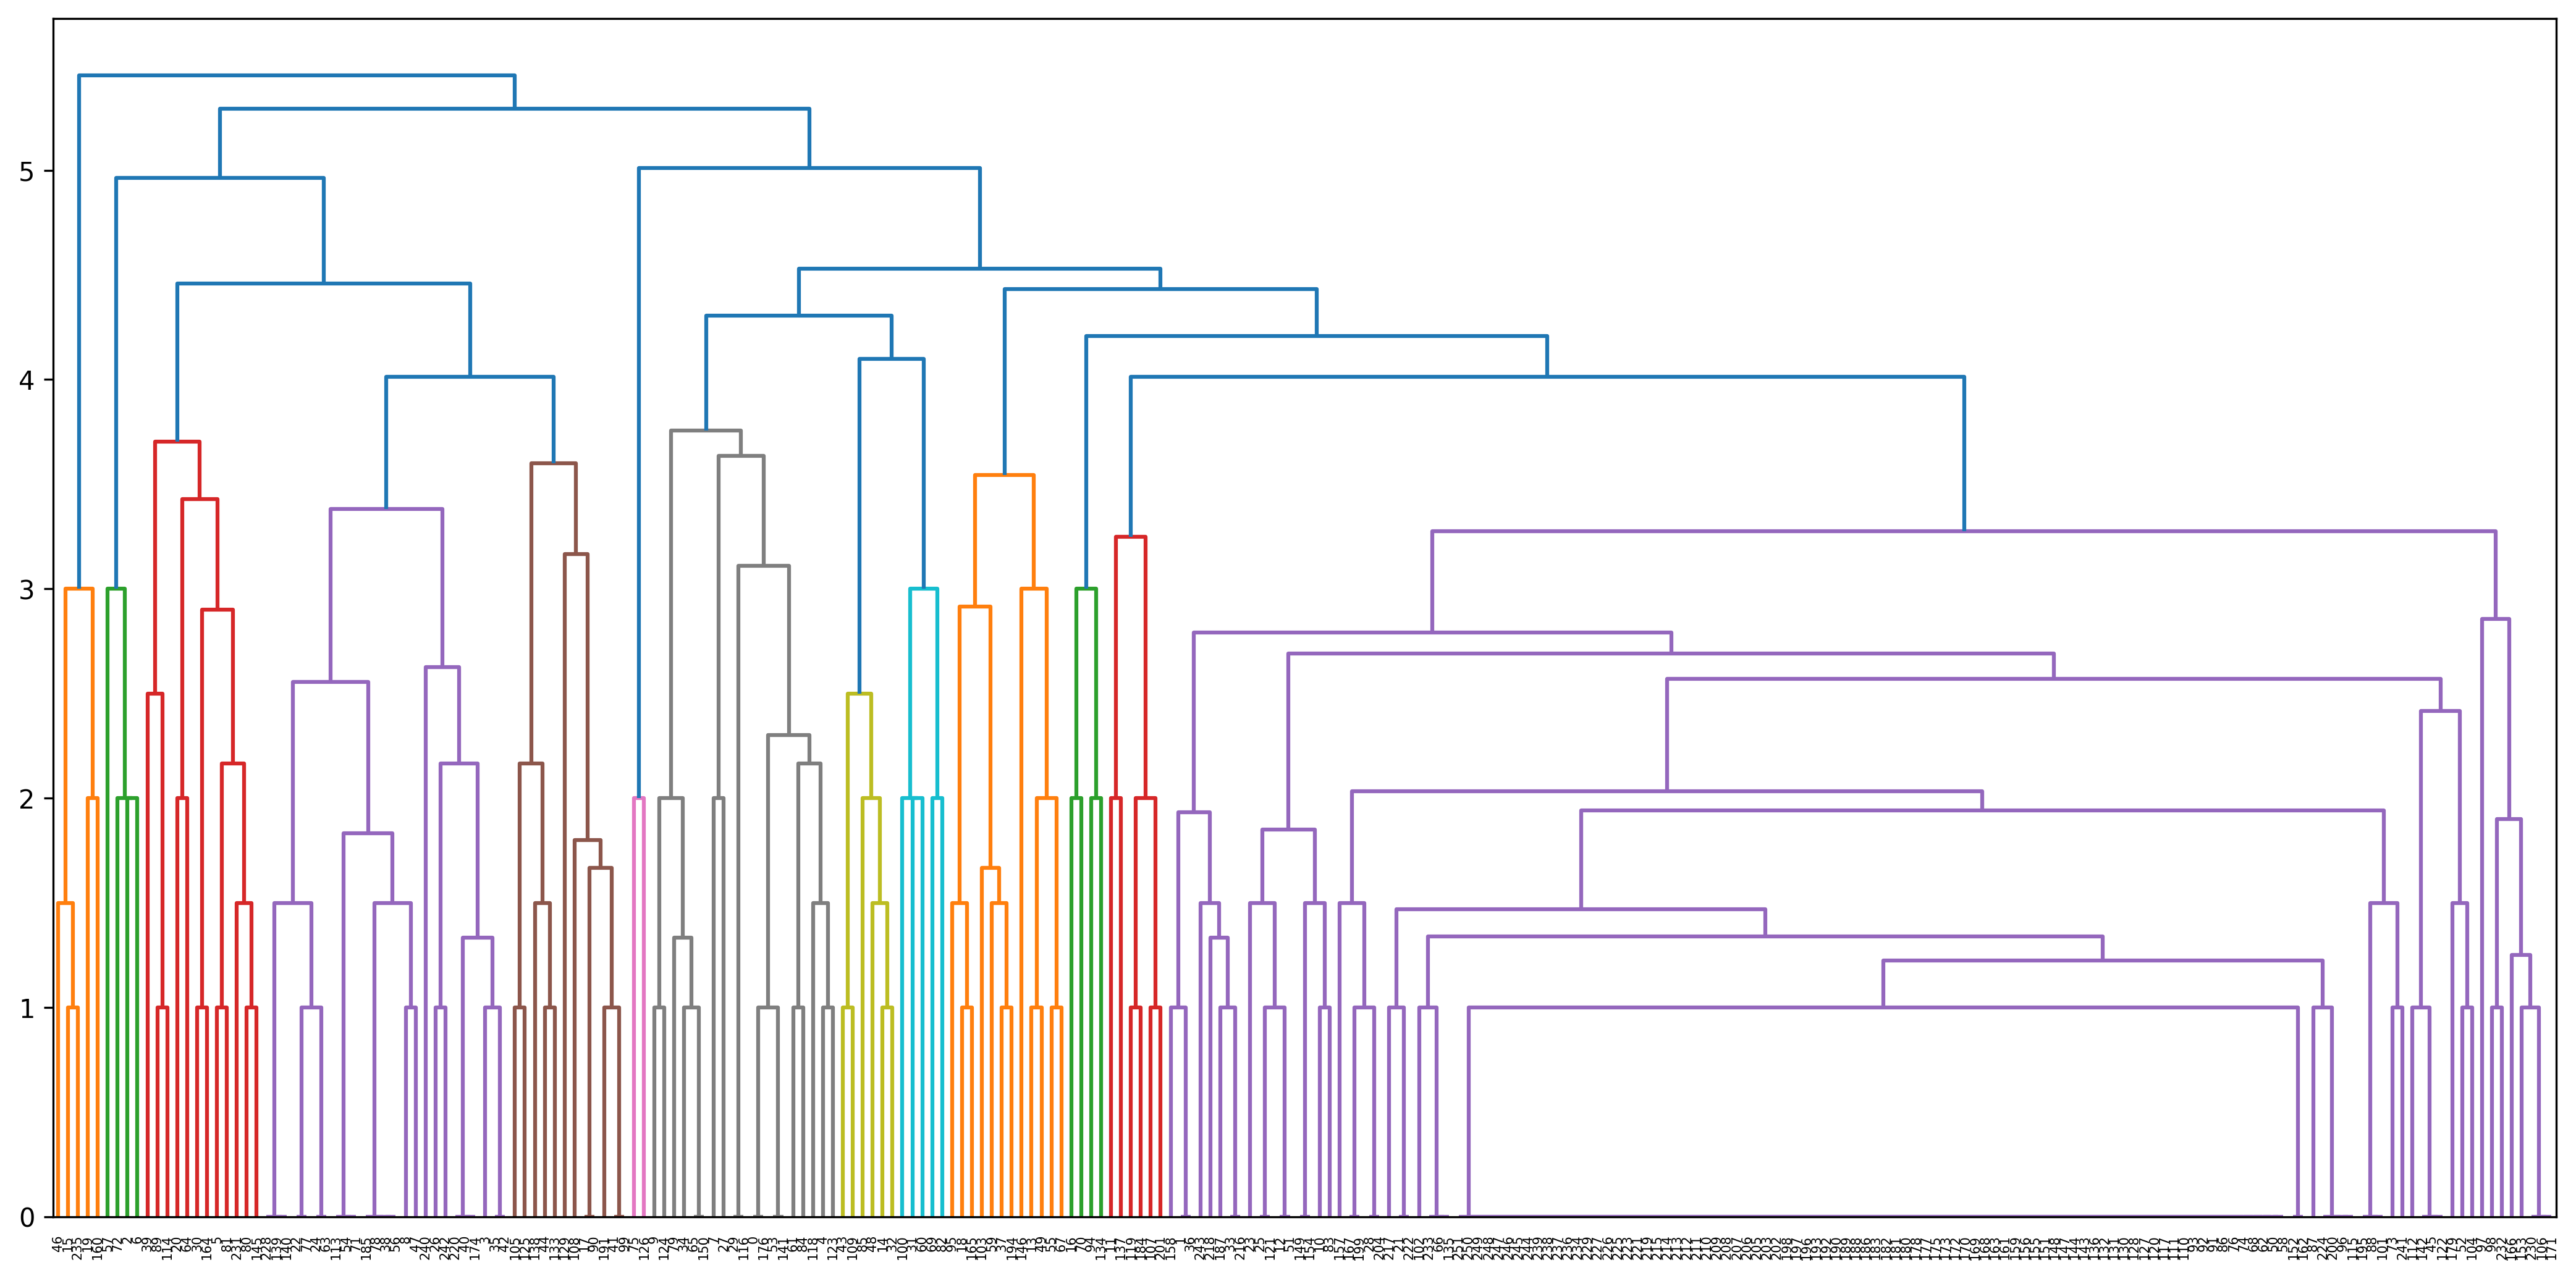
\includegraphics[width=\linewidth]{../Quantum-Annealing-for-solving-QUBO-Problems/test/Diagnostica_QALS/2/Decay_factor/ksp_1/lambda_div_3/dendrogram_2000_1.png}
\caption{Agglomerative Clustering Dendogram}
\label{fig:AgglomerativeClustering-ksp1}
\end{figure}

\clearpage
\subsection{ksp\_3}

\begin{table}[h]
\centering
\begin{tabular}{lcc}
\hline
\textbf{Metrica} & \(\lambda_1\) & \(\lambda_2\) \\
\hline
Numero cluster & 34 & 36 \\
Dimensione cluster massimo & 74 & 89 \\
Cluster z best & 27 & 3 \\
Single clusters & 1 & 0 \\
\(f_Q\) medoid & 307680.74 & 9569403810.67 \\
Profit medoid & 4495 & 4056 \\
Weight medoid & 3988 & 2402 \\
\hline
\(f_Q\) Min Found QALS & 31096.64 & 6043281857.67 \\
Profit Found QALS & 3613 & 3529 \\
Weight Found QALS & 1756 & 2042 \\
\hline
\(f_Q\) Min Found NO QALS & -9424.8 & -714267360.0 \\
Profit Found NO QALS & 2936 & 2181 \\
Weight Found NO QALS & 560 & 501 \\
\hline
\end{tabular}

\caption{Confronto dei risultati ottenuti con QALS e senza QALS.}
\label{tab:confronto-qals-noqals}
\end{table}

\begin{figure}[H]
\centering
\begin{subfigure}{0.495\textwidth}
    \centering
    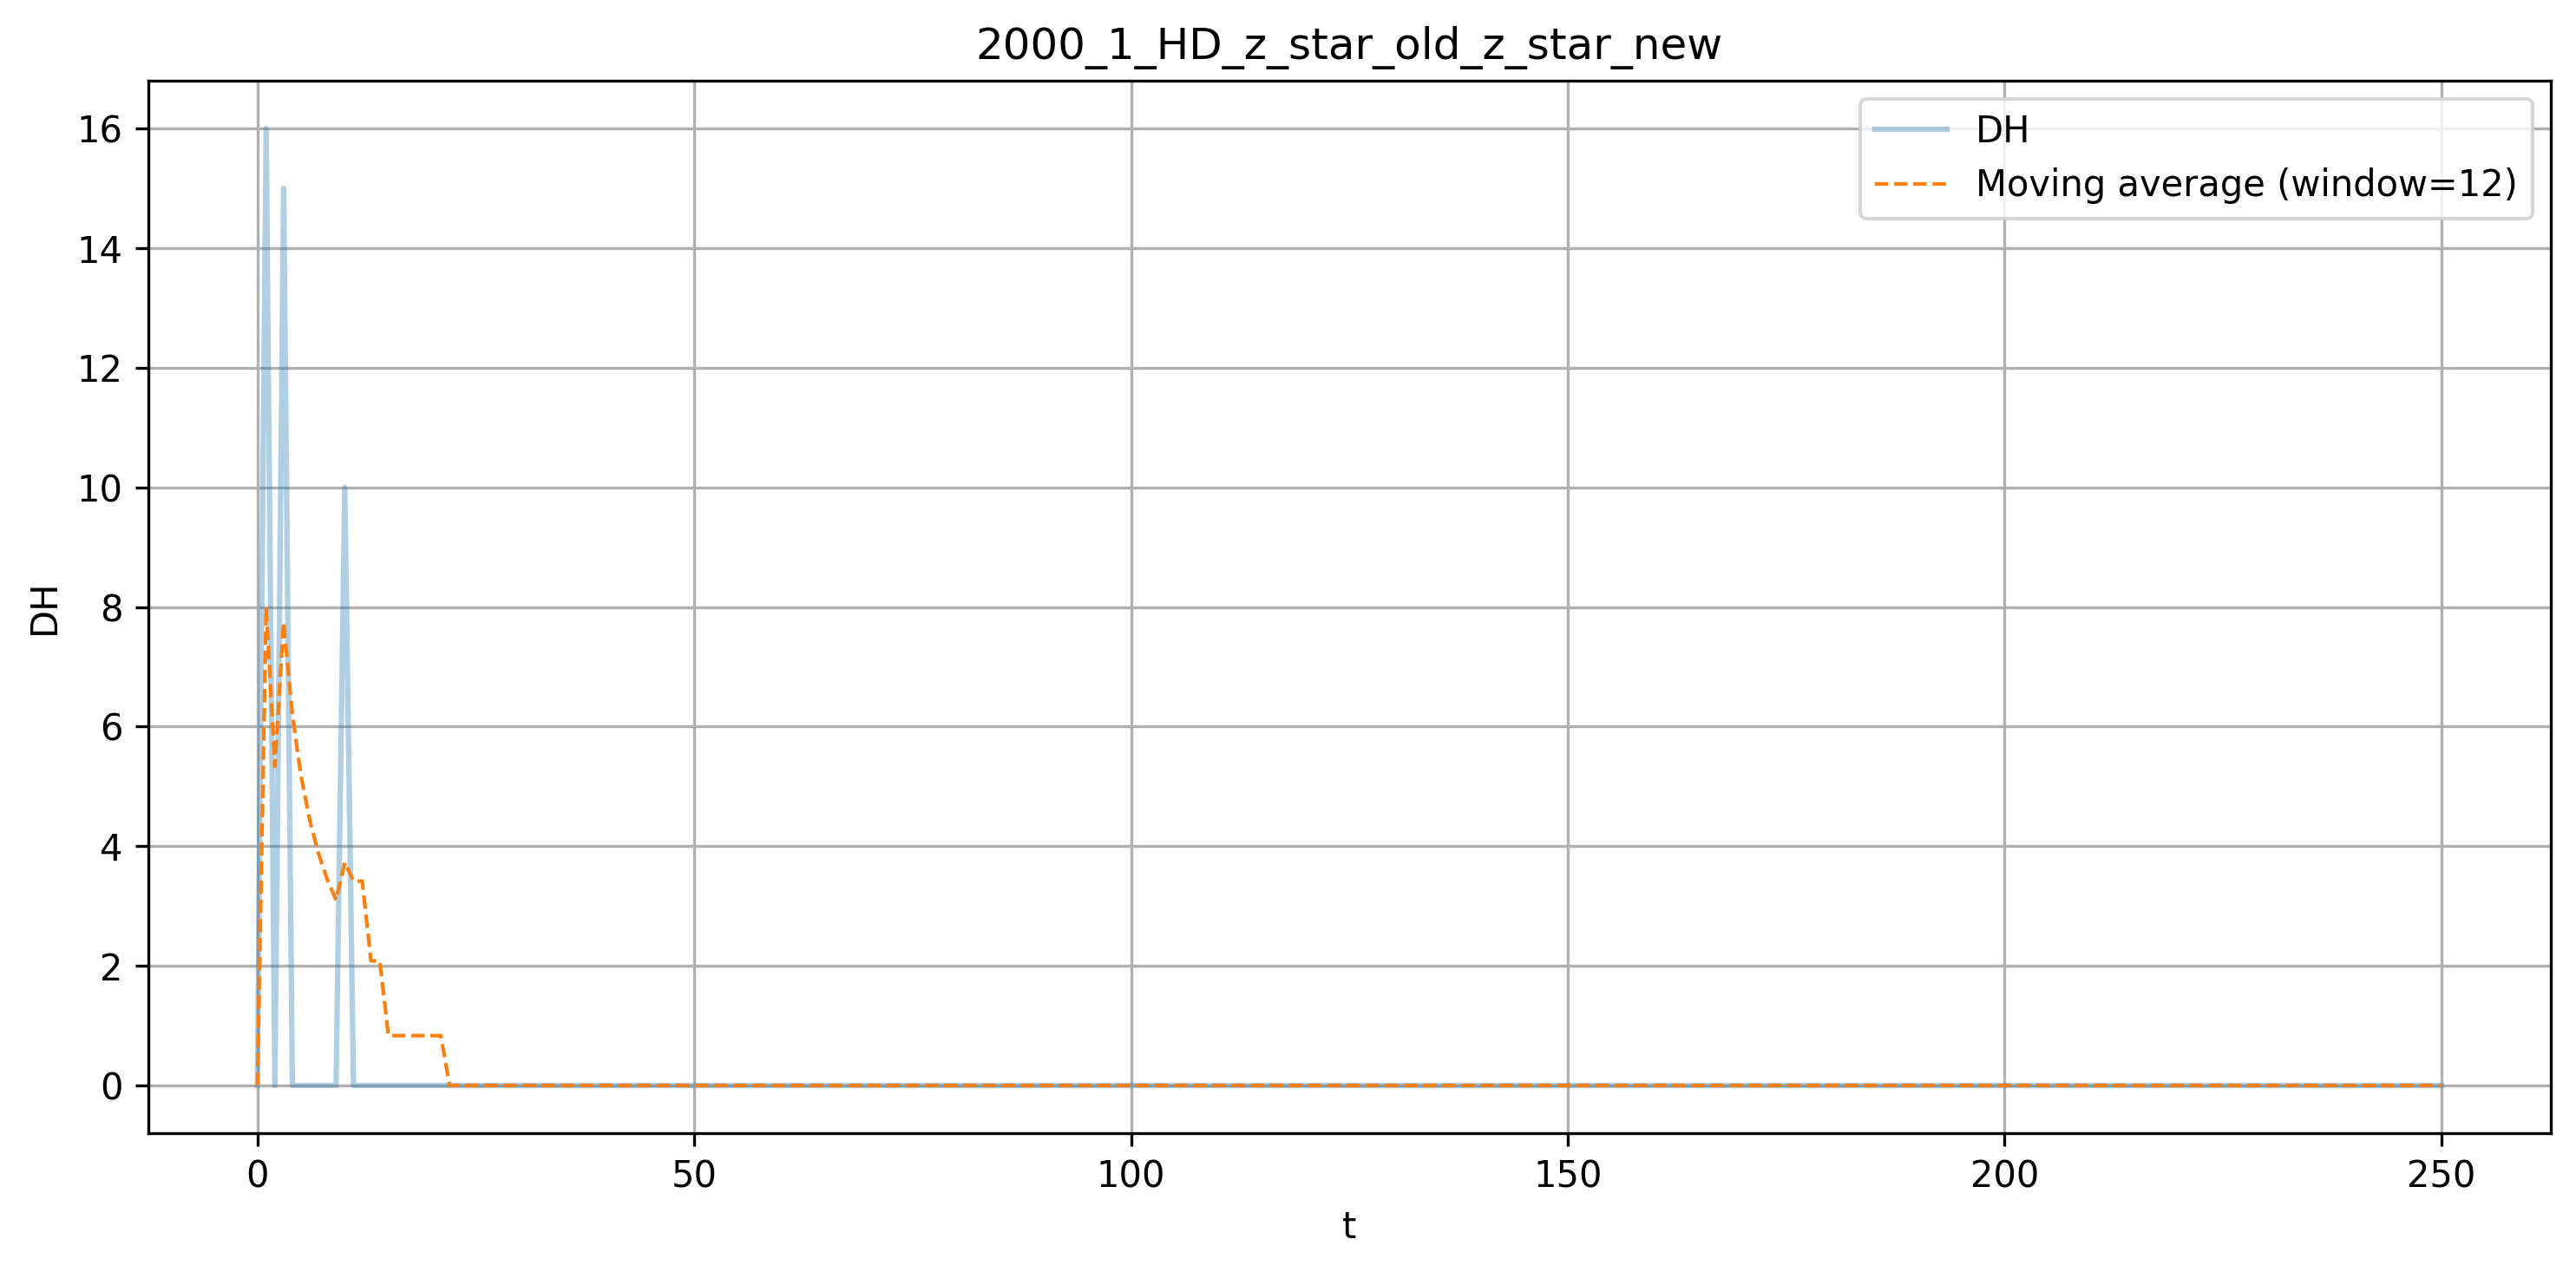
\includegraphics[width=\linewidth]{../Quantum-Annealing-for-solving-QUBO-Problems/test/Diagnostica_QALS/2/Decay_factor/ksp_3/lambda_650_dot_C/2000_1_HD_z_star_old_z_star_new.png}
    \caption{\(d_H(z_\star^{old}, z_\star^{new})\) con \(\lambda_1\)}
    \label{fig:hd-zstarold-zstarnew-lambda1}
\end{subfigure}
\hfill
\begin{subfigure}{0.495\textwidth}
    \centering
    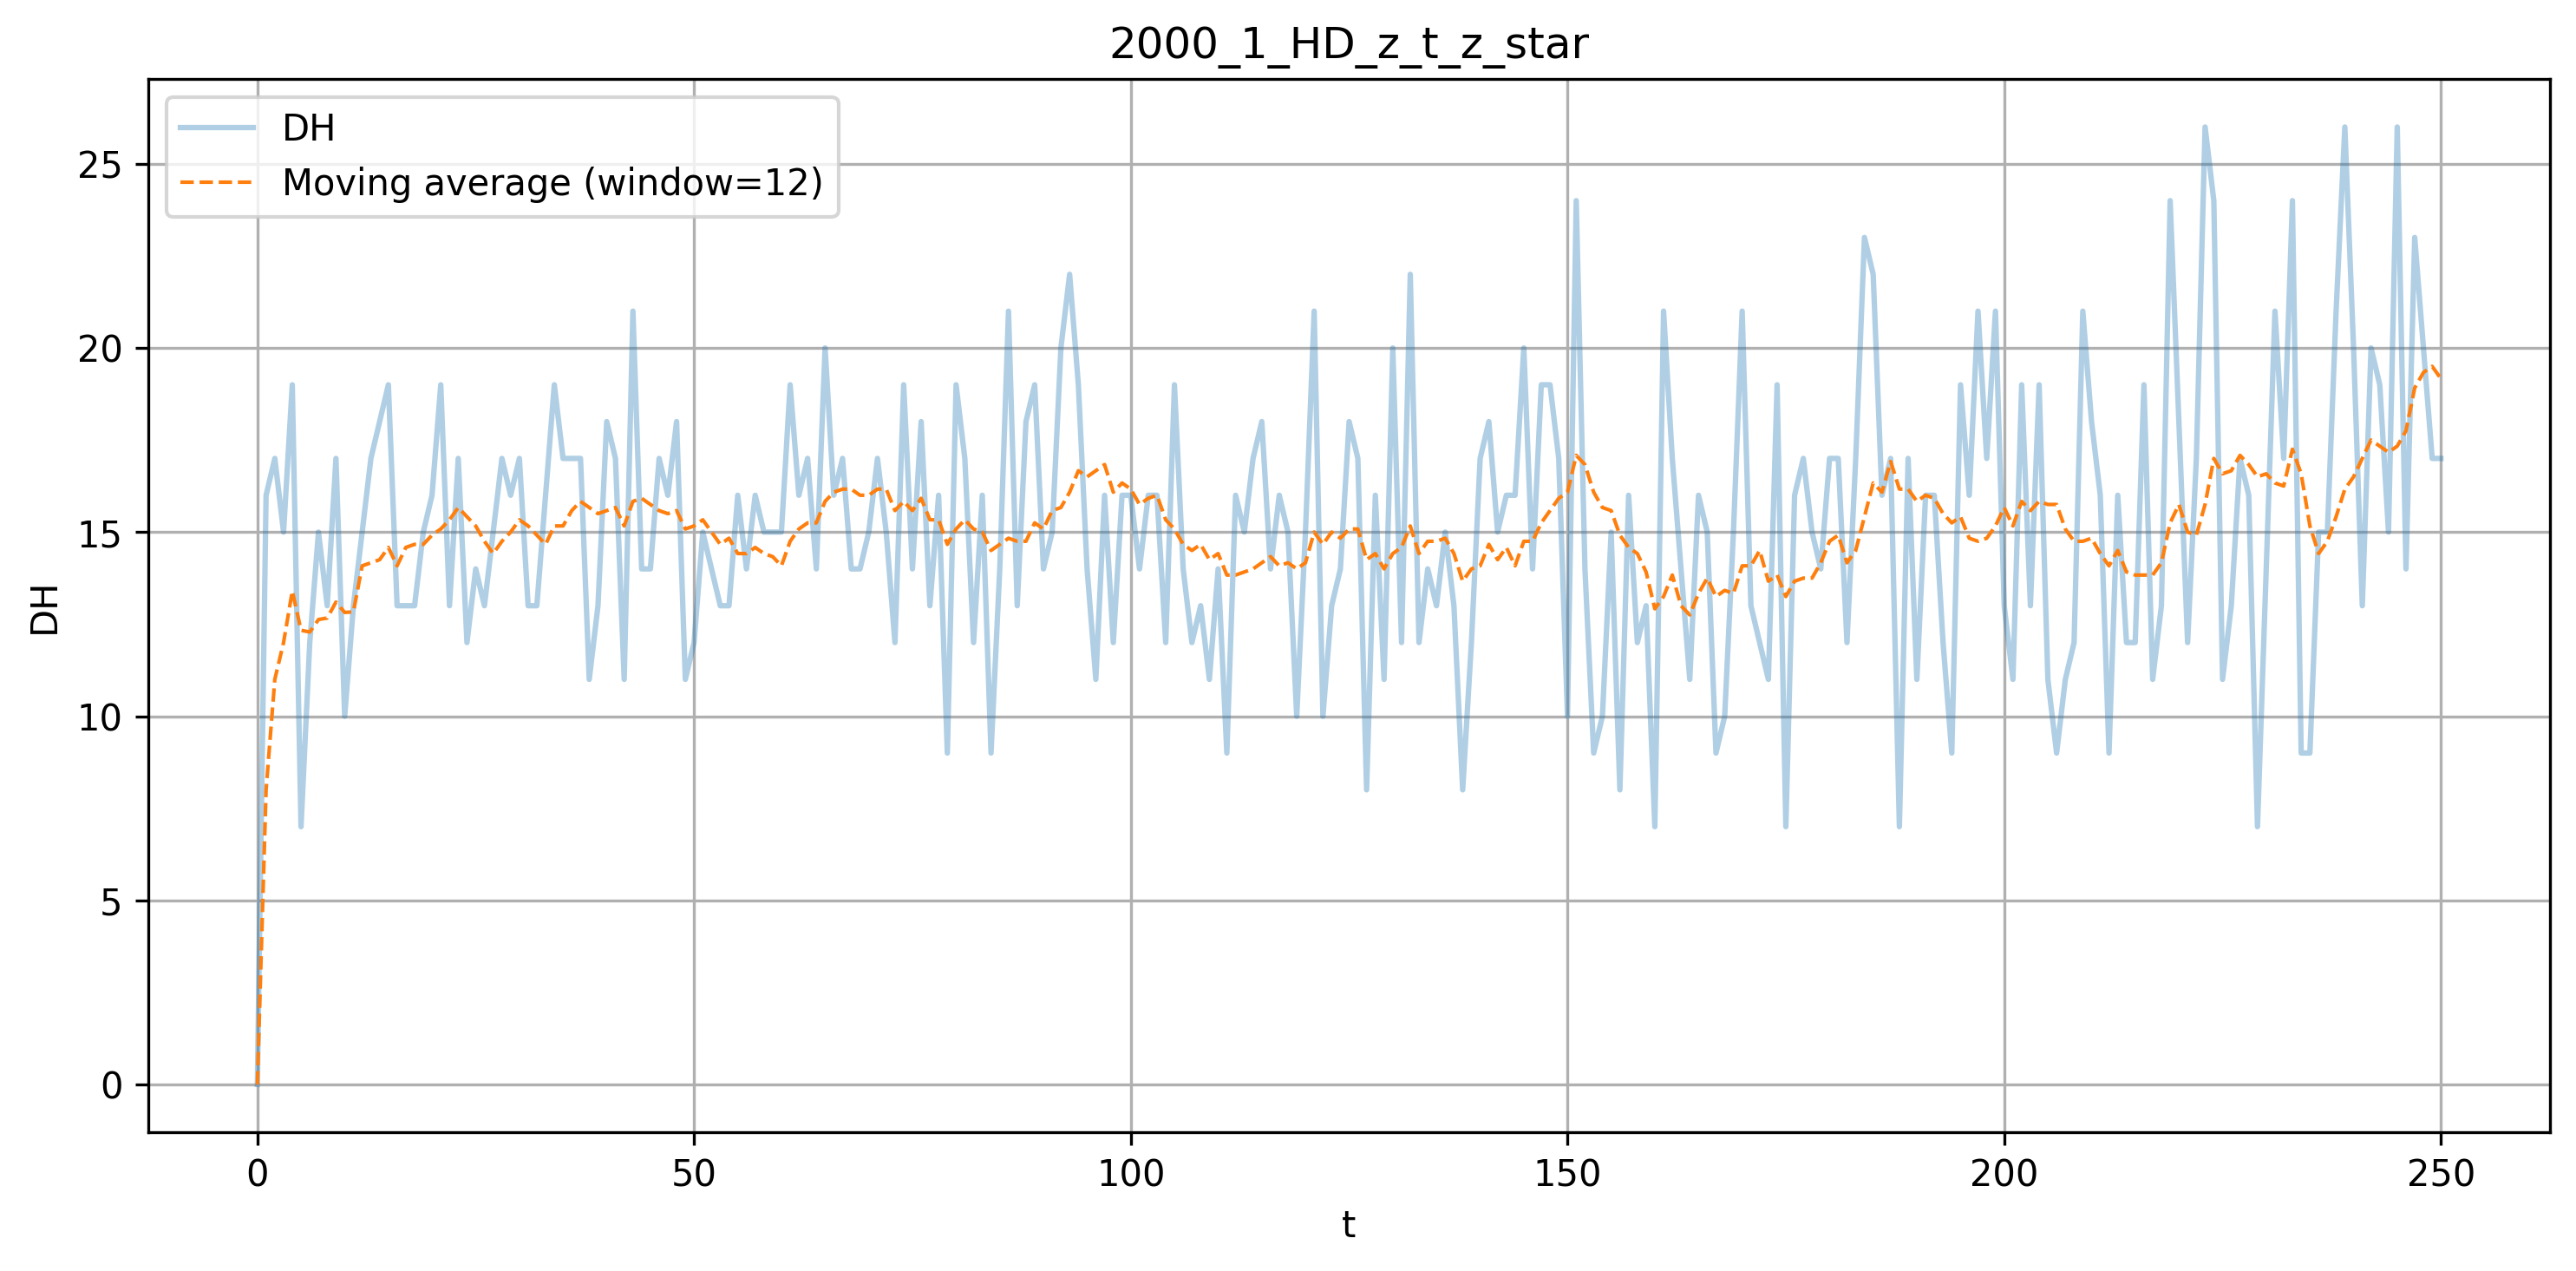
\includegraphics[width=\linewidth]{../Quantum-Annealing-for-solving-QUBO-Problems/test/Diagnostica_QALS/2/Decay_factor/ksp_3/lambda_650_dot_C/2000_1_HD_z_t_z_star.png}
    \caption{\(d_H(z_t, z_\star)\) con \(\lambda_1\)}
    \label{fig:hd-zt-zstar-lambda1}
\end{subfigure}

\vspace{0.35cm}

\begin{subfigure}{0.495\textwidth}
    \centering
    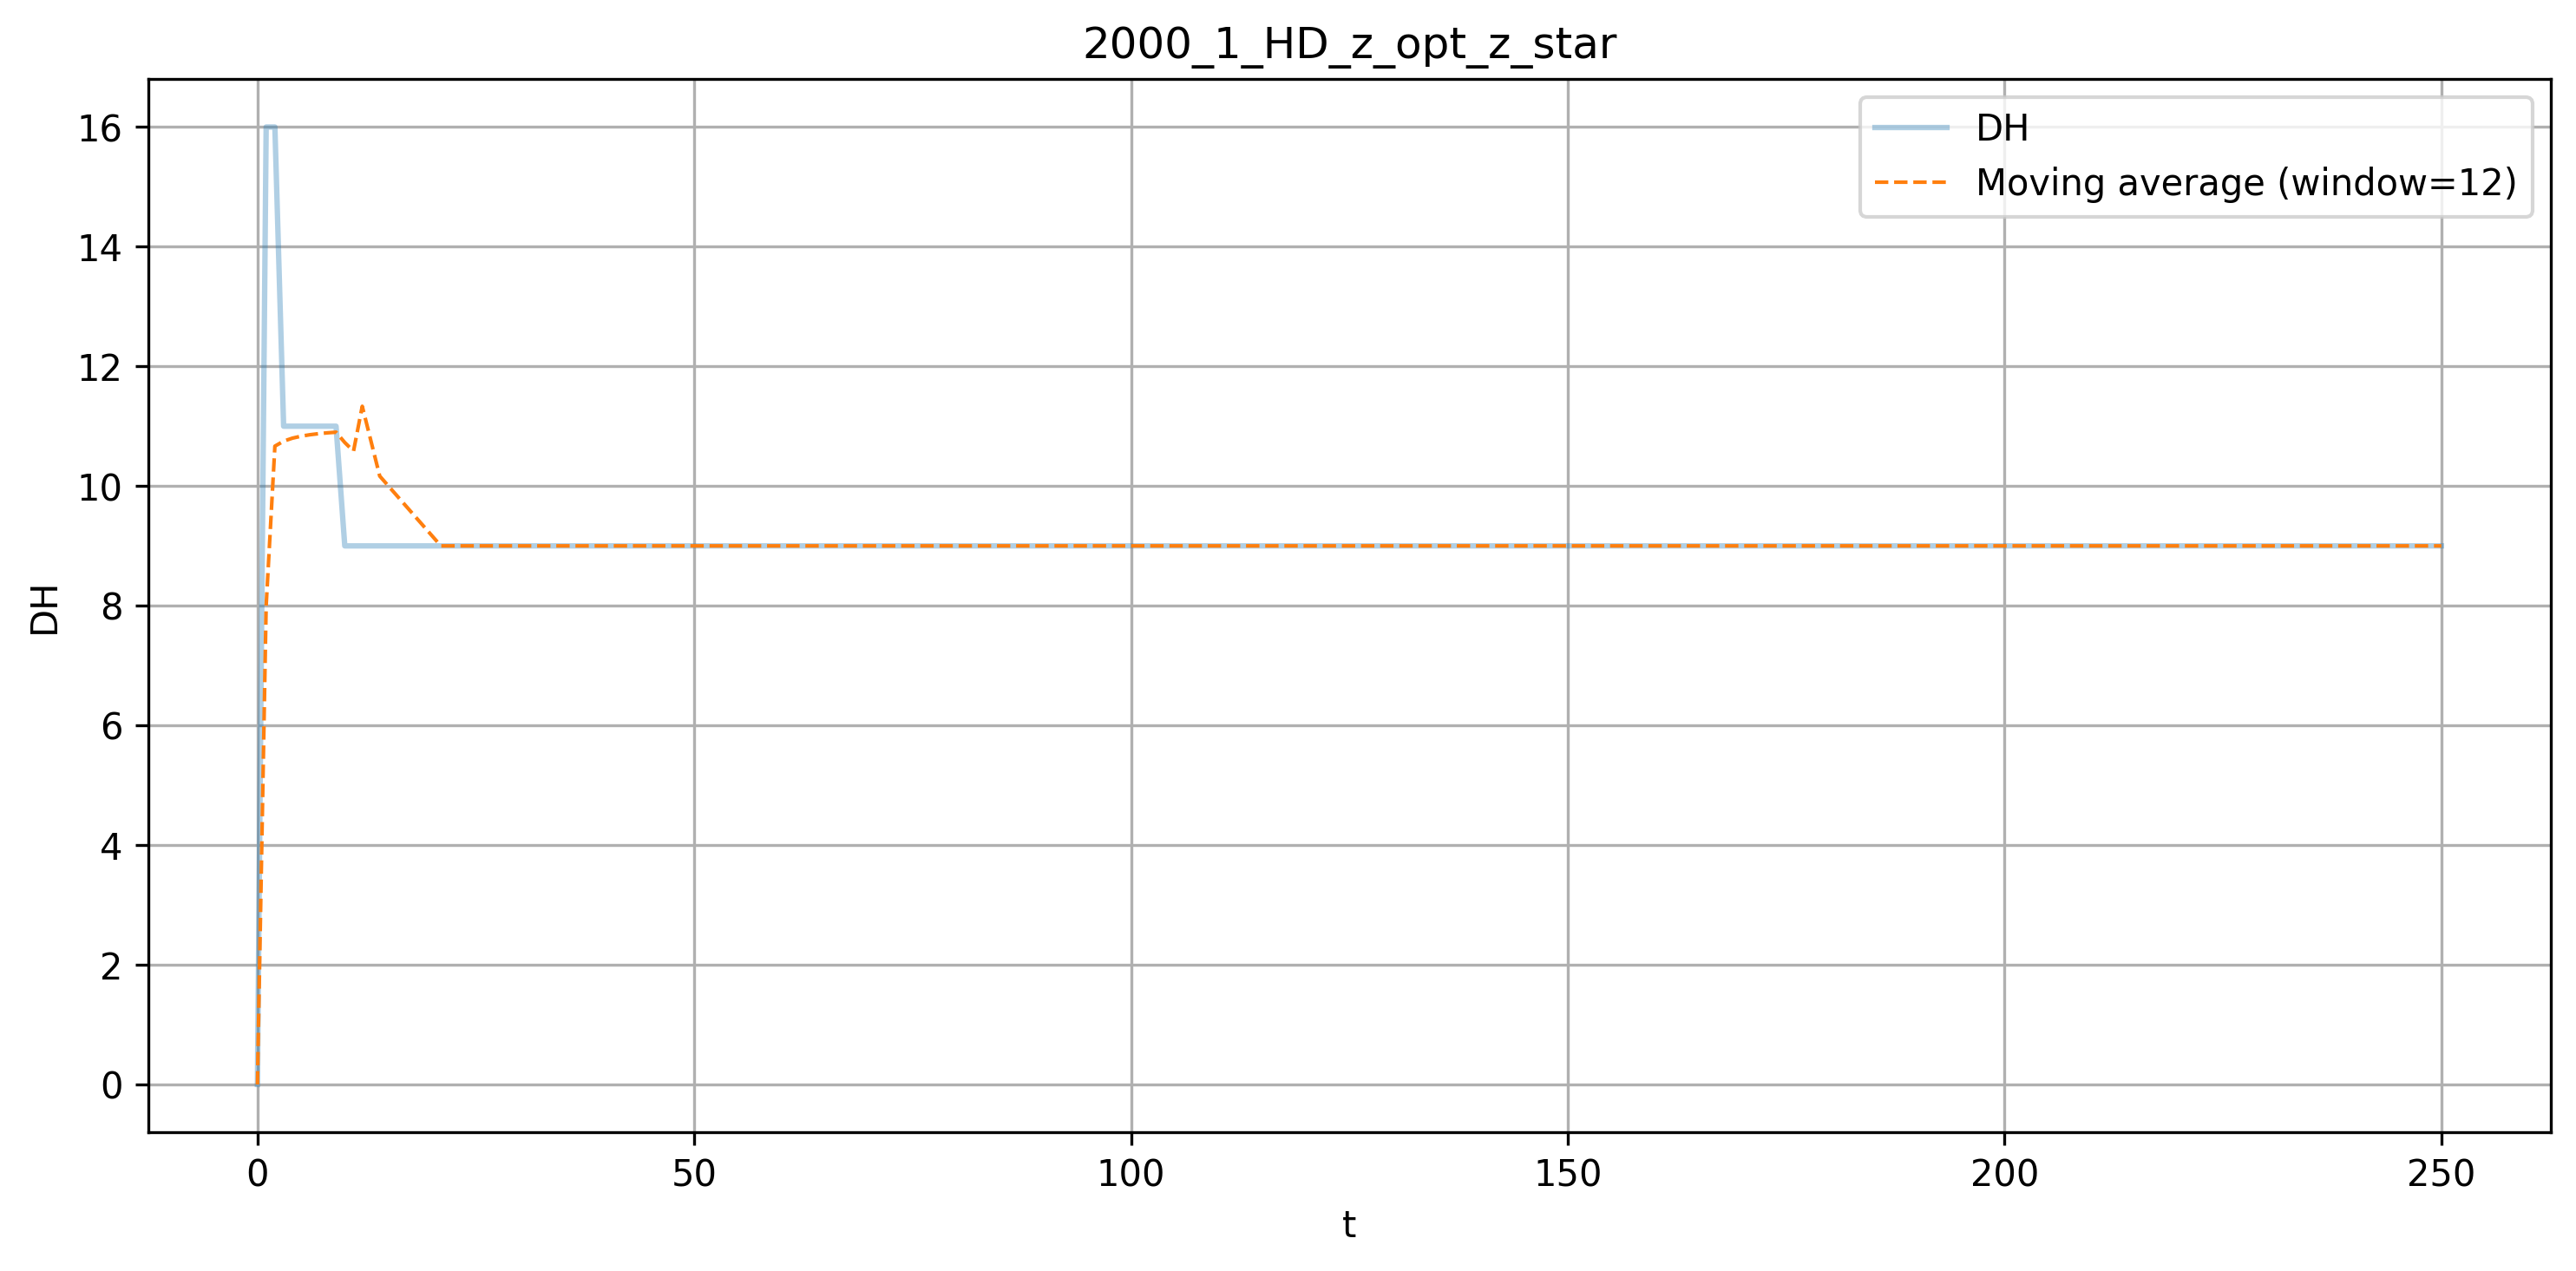
\includegraphics[width=\linewidth]{../Quantum-Annealing-for-solving-QUBO-Problems/test/Diagnostica_QALS/2/Decay_factor/ksp_3/lambda_650_dot_C/2000_1_HD_z_opt_z_star.png}
    \caption{\(d_H(z_{opt}, z_\star)\) con \(\lambda_1\)}
    \label{fig:hd-zopt-zstar-lambda1}
\end{subfigure}
\hfill
\begin{subfigure}{0.495\textwidth}
    \centering
    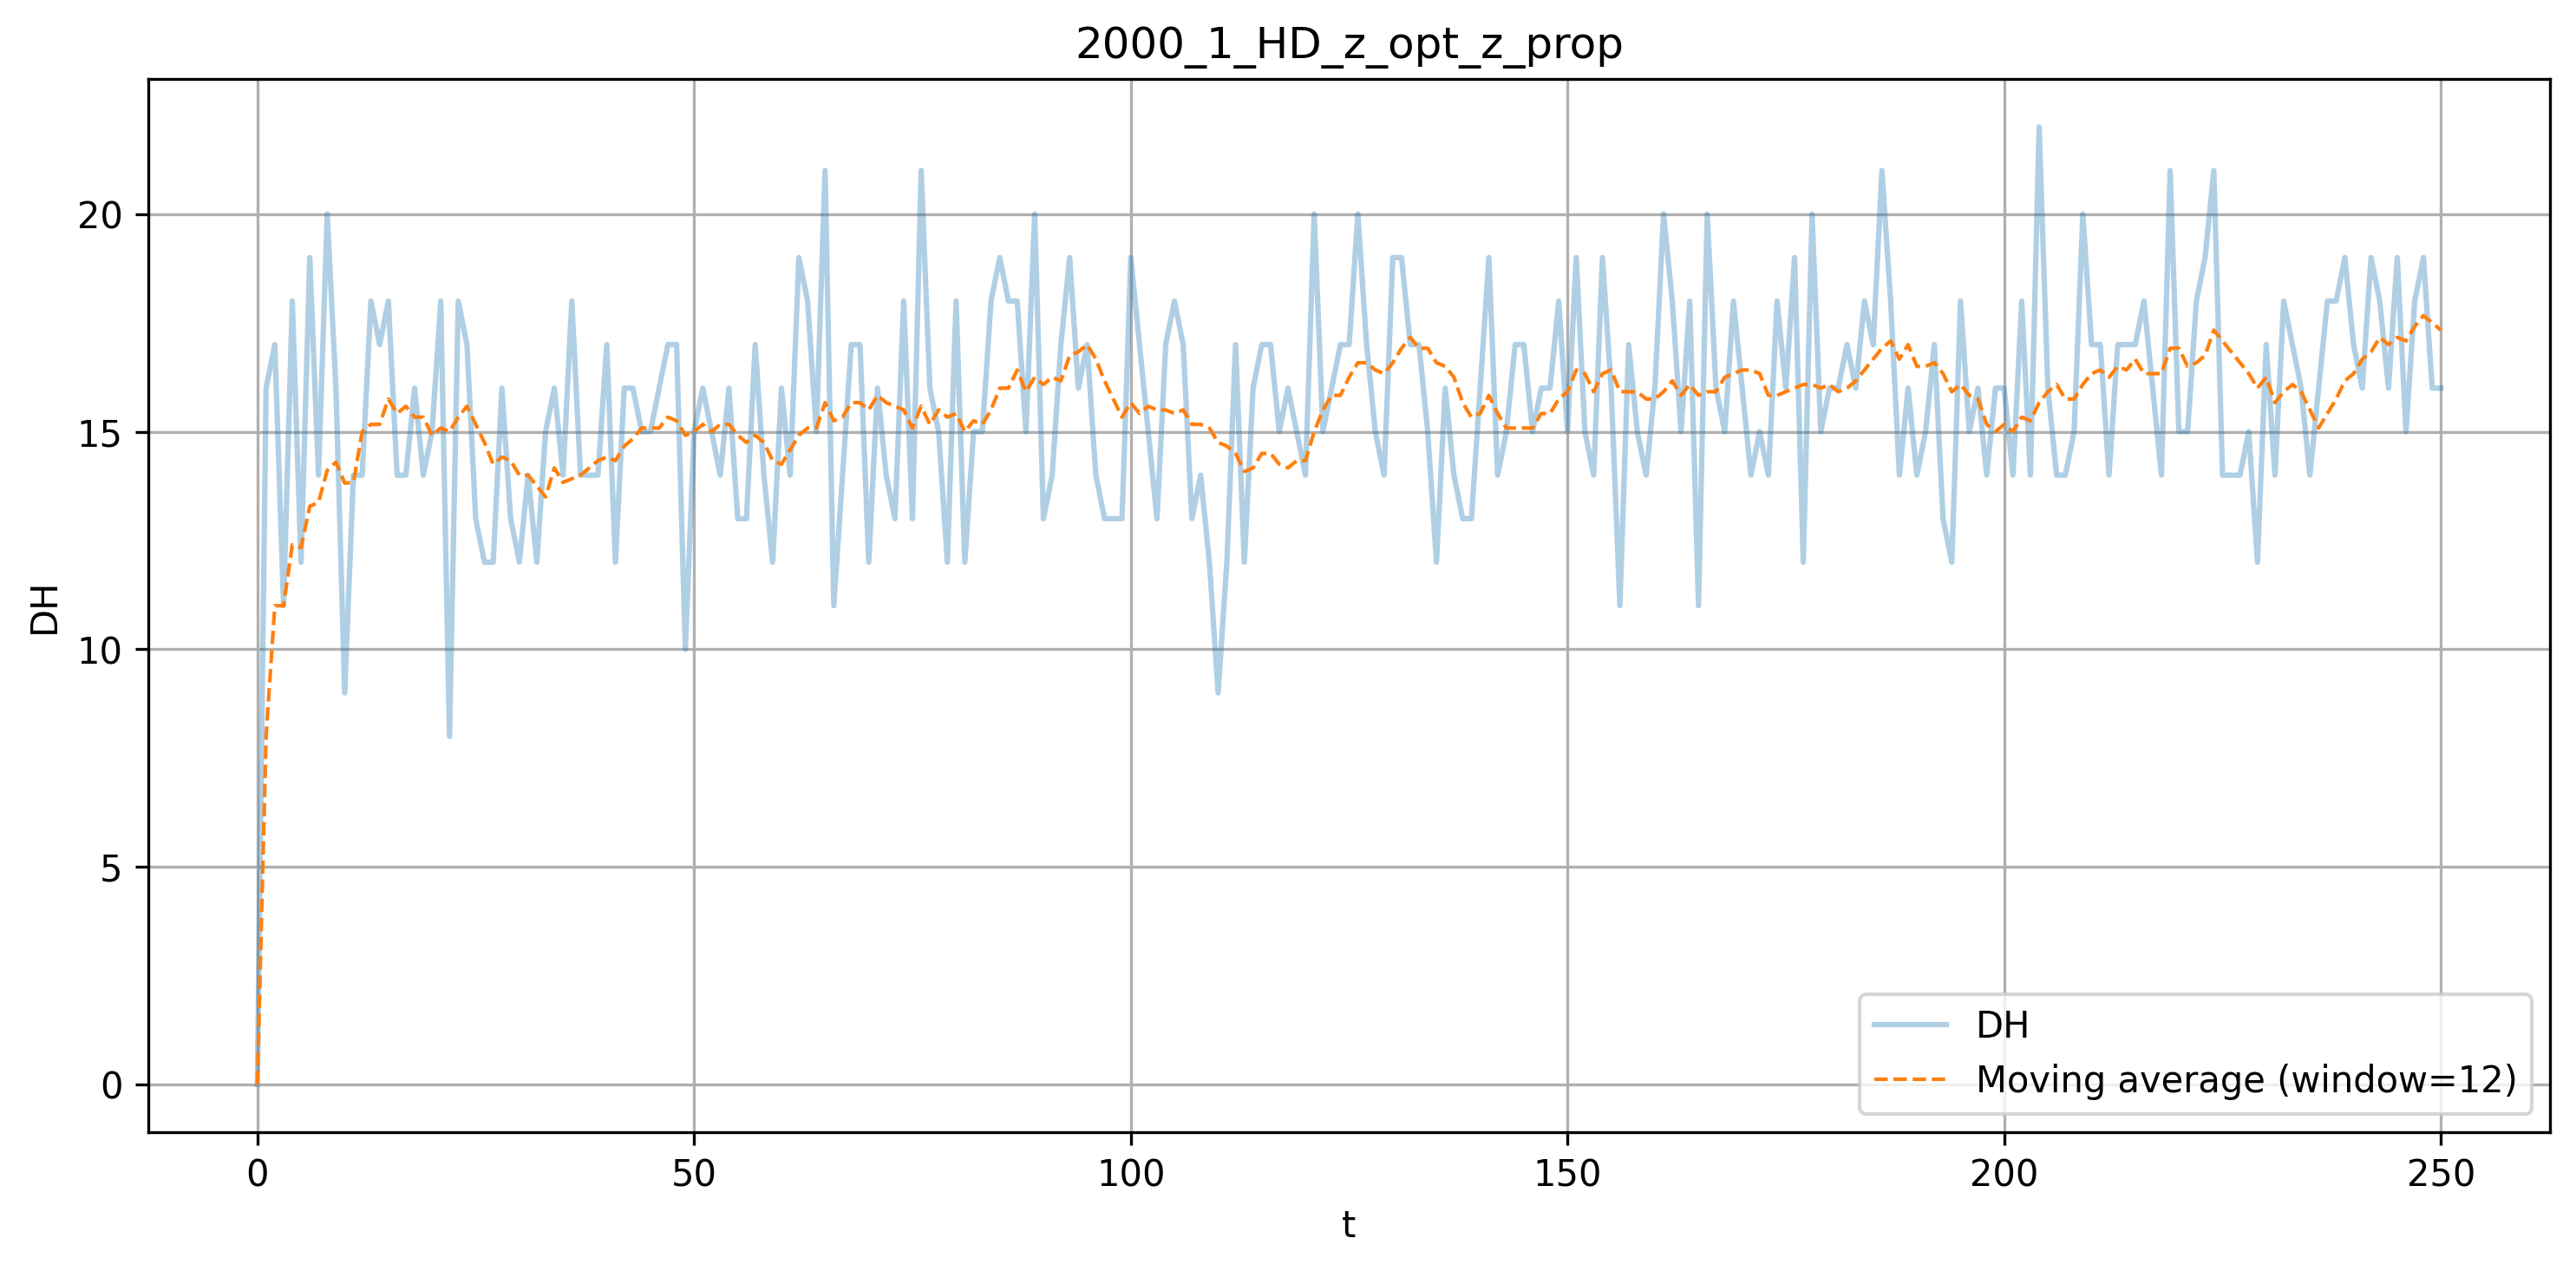
\includegraphics[width=\linewidth]{../Quantum-Annealing-for-solving-QUBO-Problems/test/Diagnostica_QALS/2/Decay_factor/ksp_3/lambda_650_dot_C/2000_1_HD_z_opt_z_prop.png}
    \caption{\(d_H(z_{opt}, z_t)\) con \(\lambda_1\)}
    \label{fig:hd-zopt-zt-lambda1}
\end{subfigure}

\vspace{0.35cm}

\begin{subfigure}{0.495\textwidth}
    \centering
    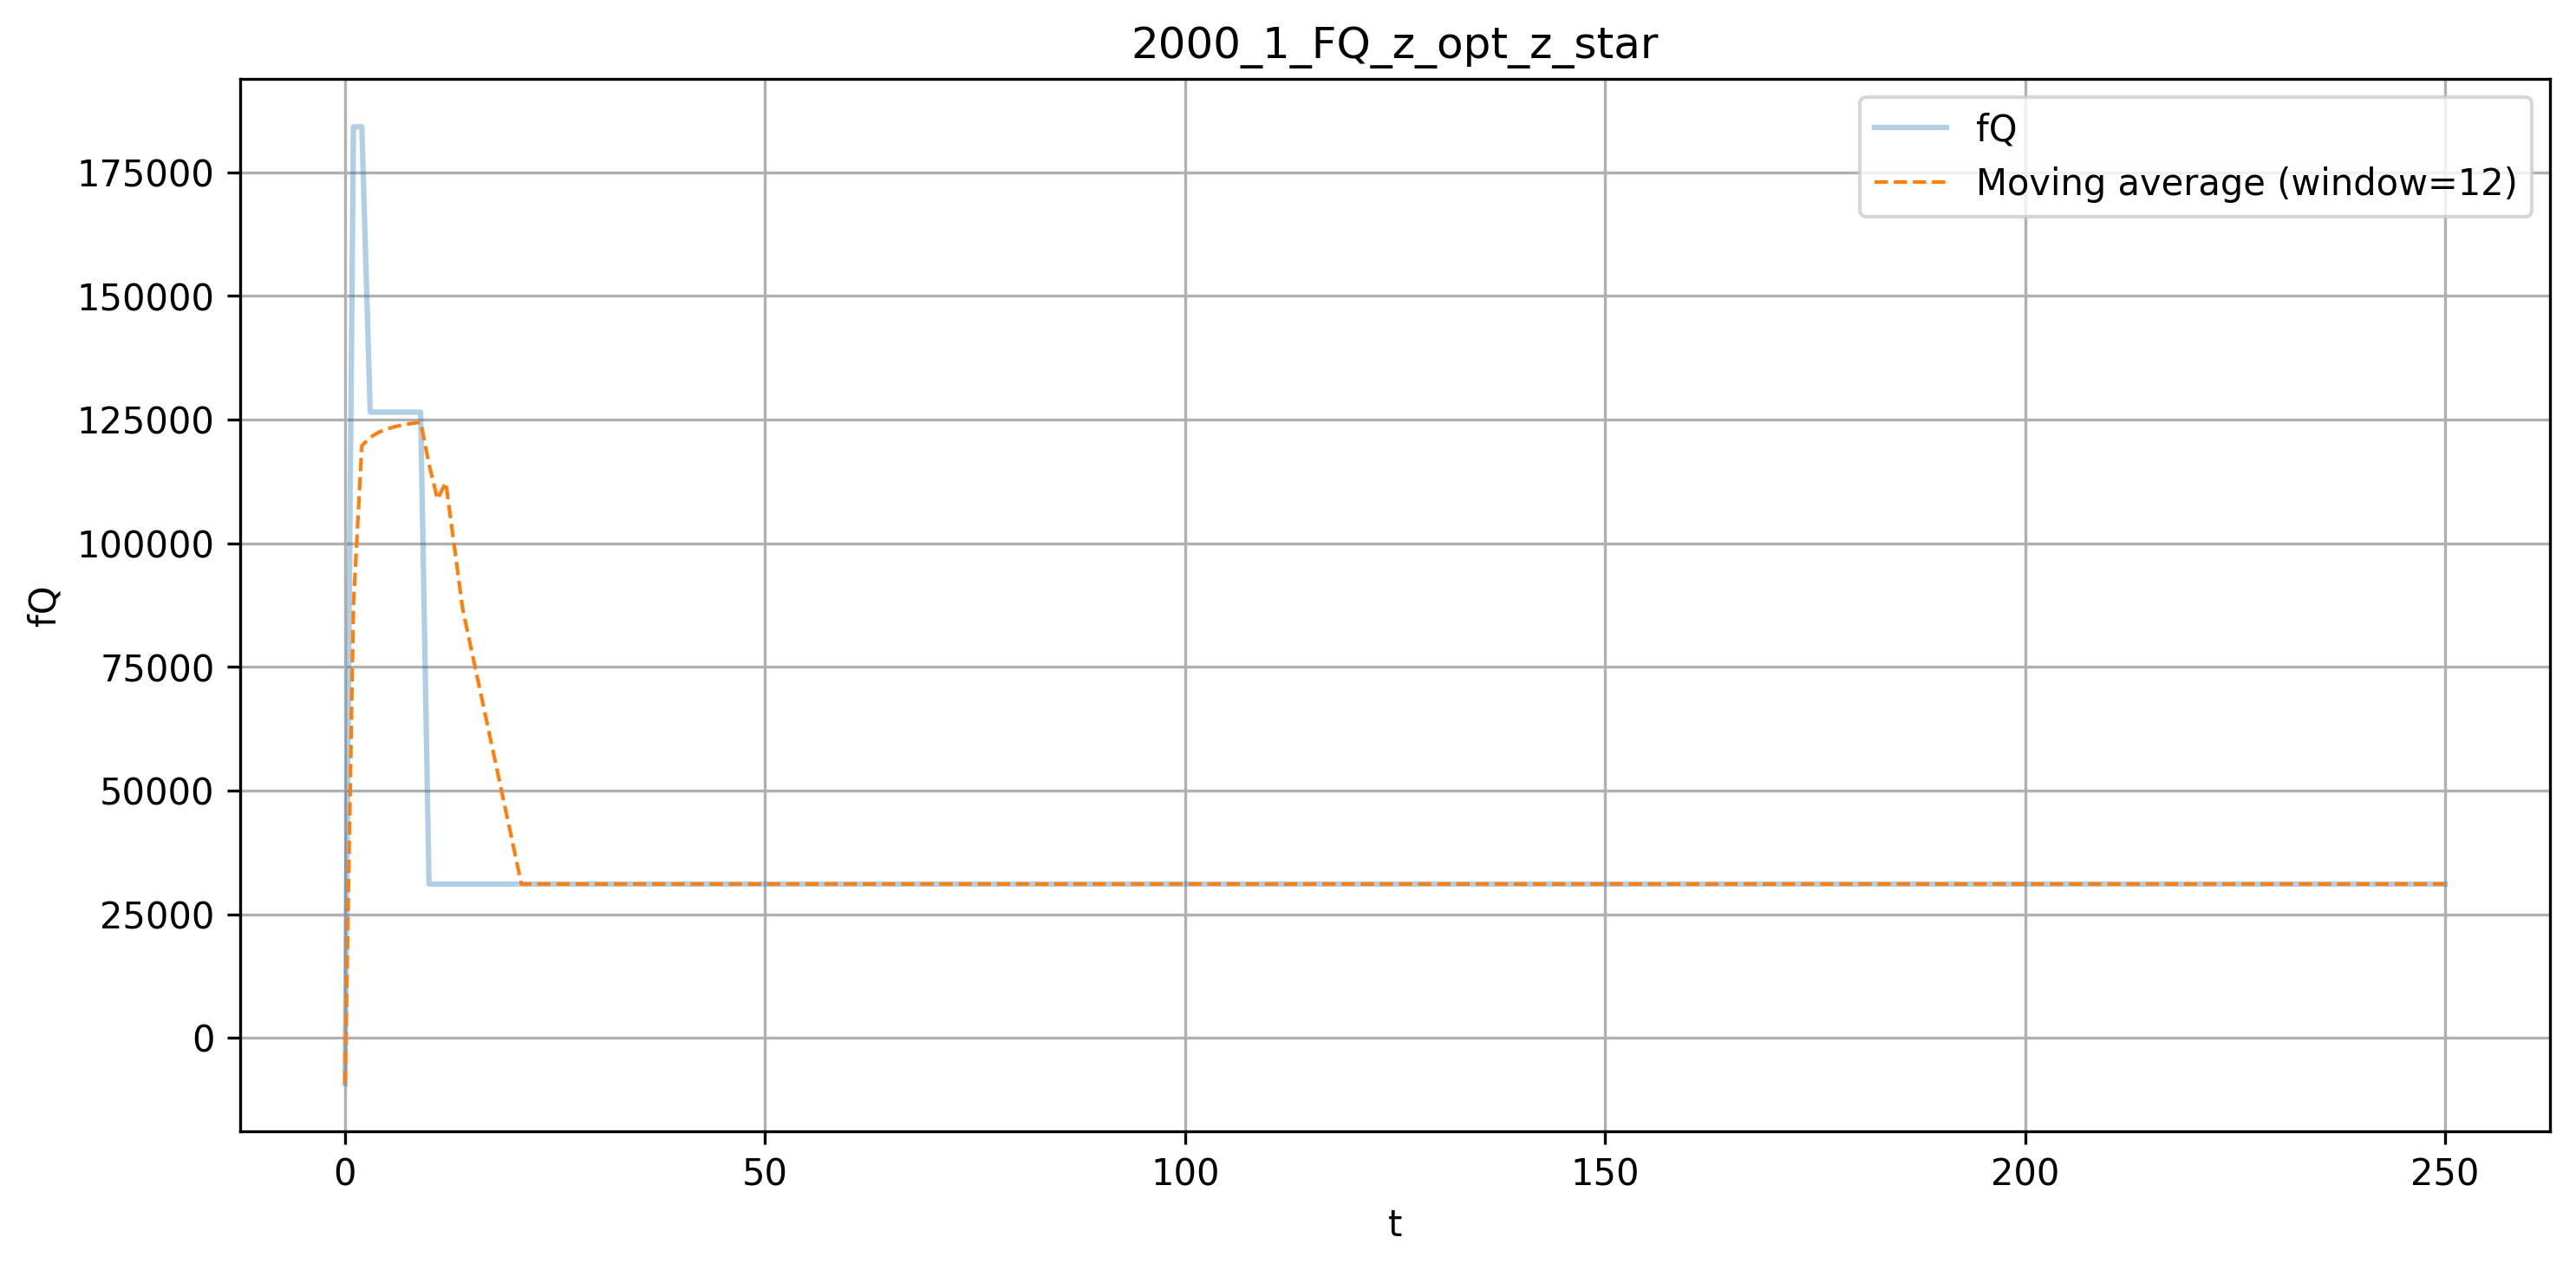
\includegraphics[width=\linewidth]{../Quantum-Annealing-for-solving-QUBO-Problems/test/Diagnostica_QALS/2/Decay_factor/ksp_3/lambda_650_dot_C/2000_1_FQ_z_opt_z_star.png}
    \caption{\(f_Q(z_\star)\) con \(\lambda_1\)}
    \label{fig:fQ-zstar-lambda1}
\end{subfigure}
\hfill
\begin{subfigure}{0.495\textwidth}
    \centering
    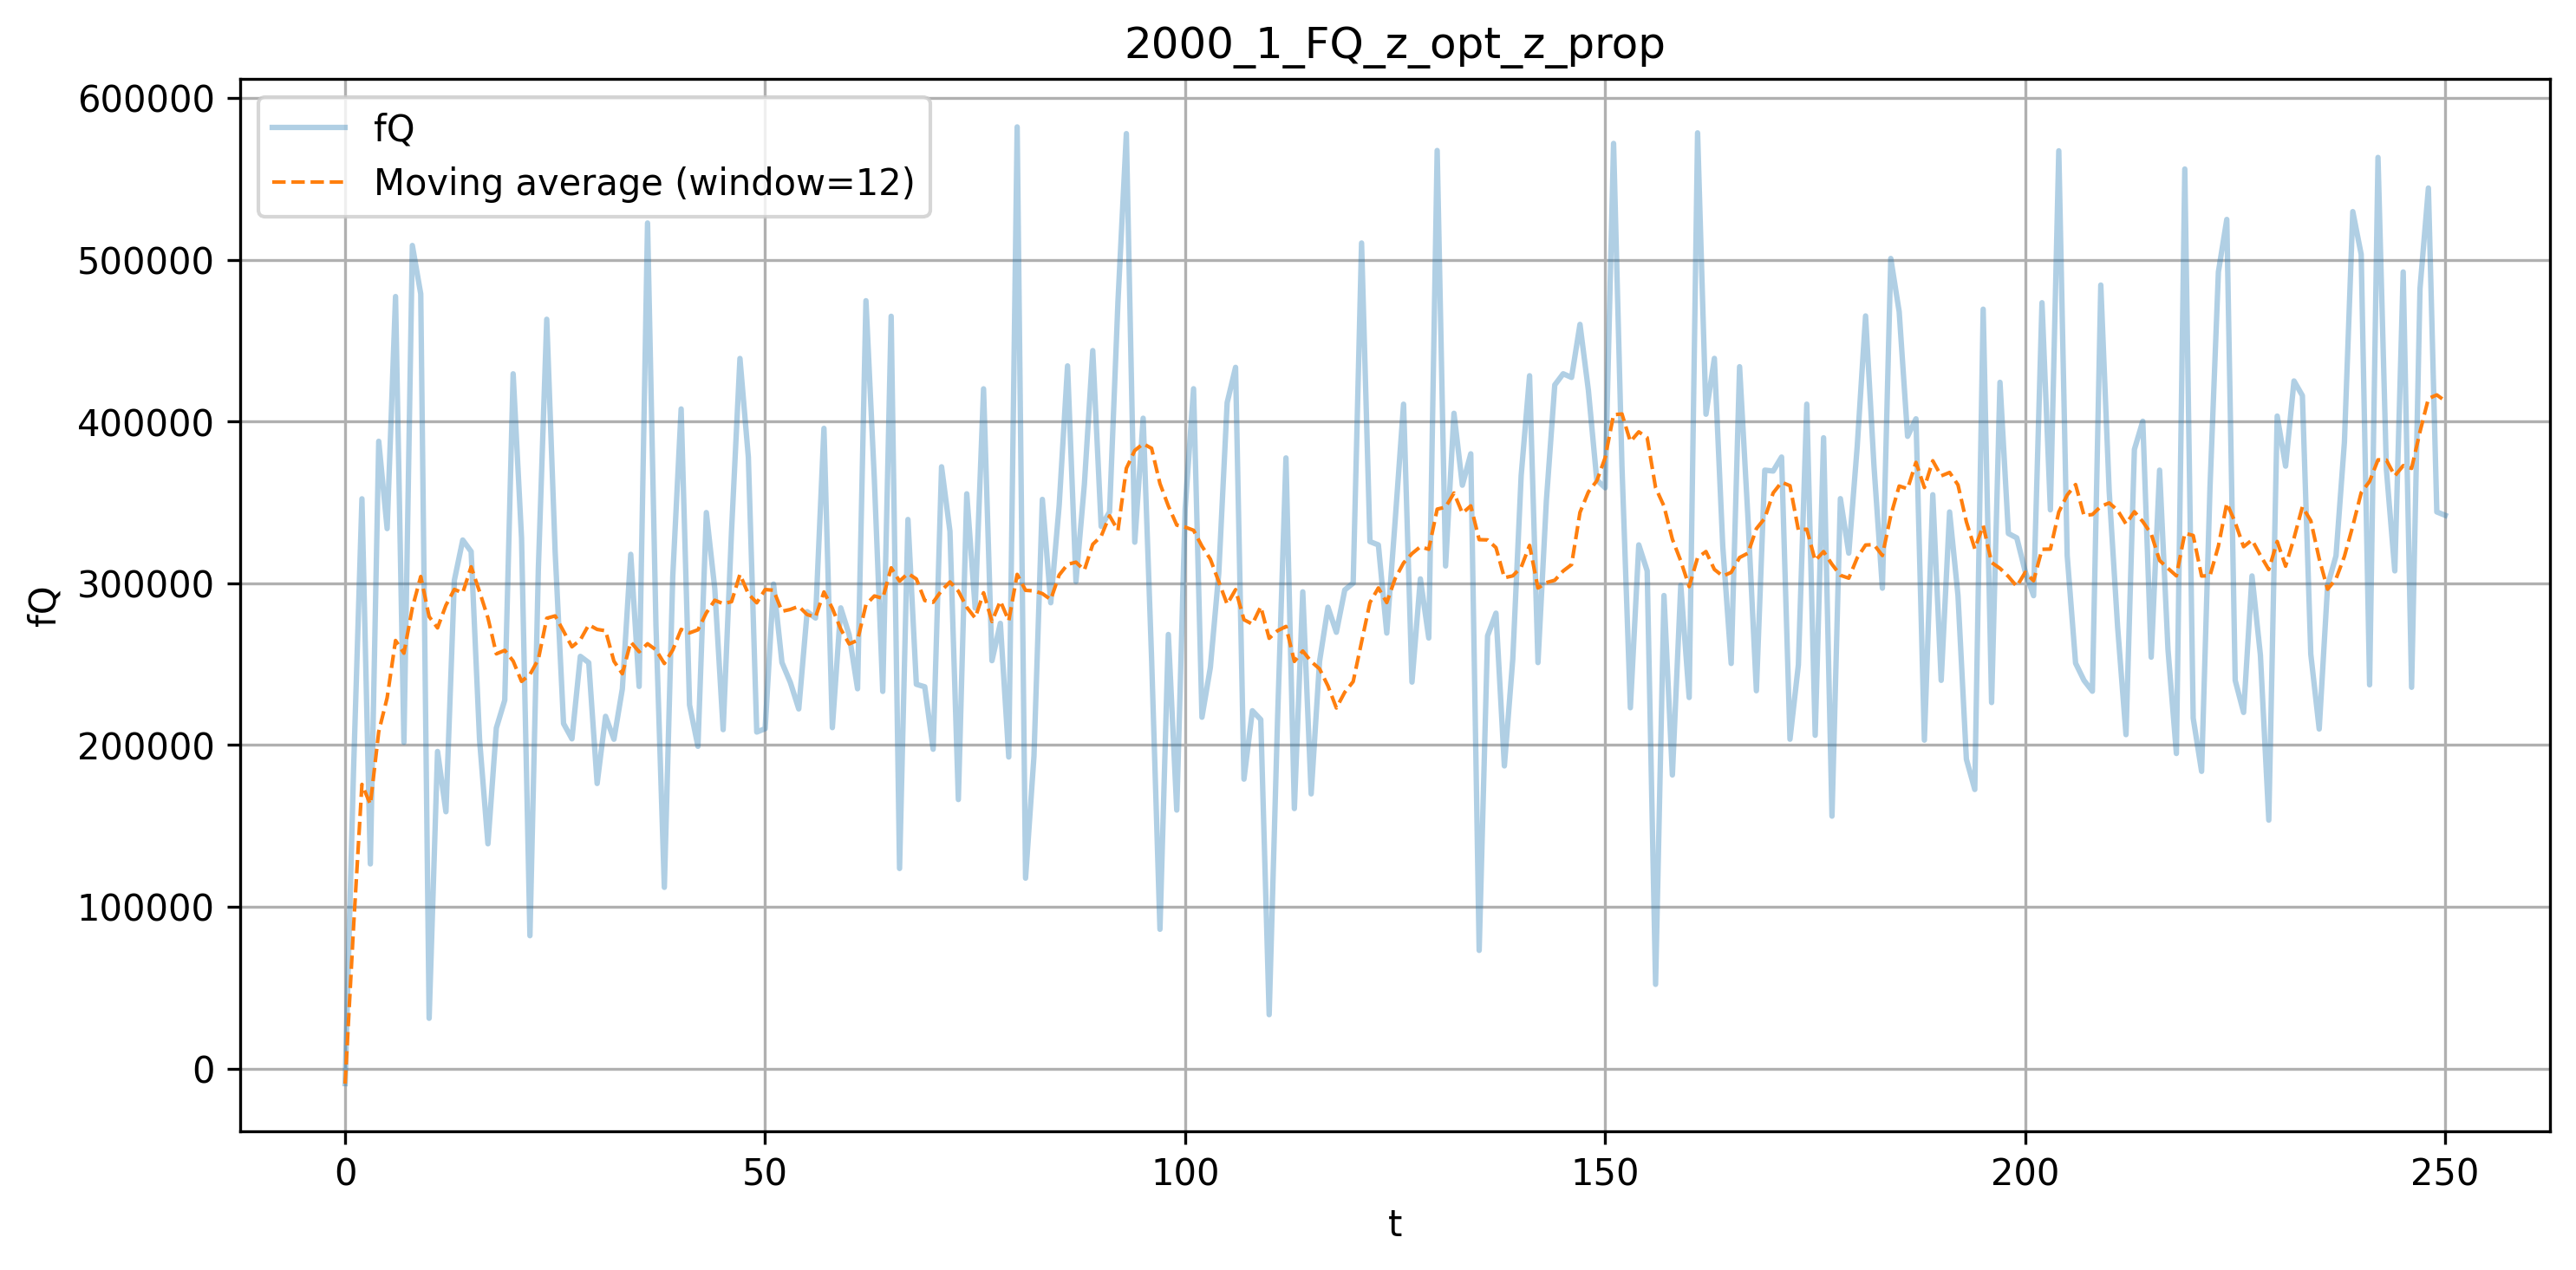
\includegraphics[width=\linewidth]{../Quantum-Annealing-for-solving-QUBO-Problems/test/Diagnostica_QALS/2/Decay_factor/ksp_3/lambda_650_dot_C/2000_1_FQ_z_opt_z_prop.png}
    \caption{\(f_Q(z_t)\) con \(\lambda_1\)}
    \label{fig:fQ-zt-lambda1}
\end{subfigure}
\label{fig:confronto-hamming-ksp31}
\end{figure}

\begin{figure}[H]
\centering
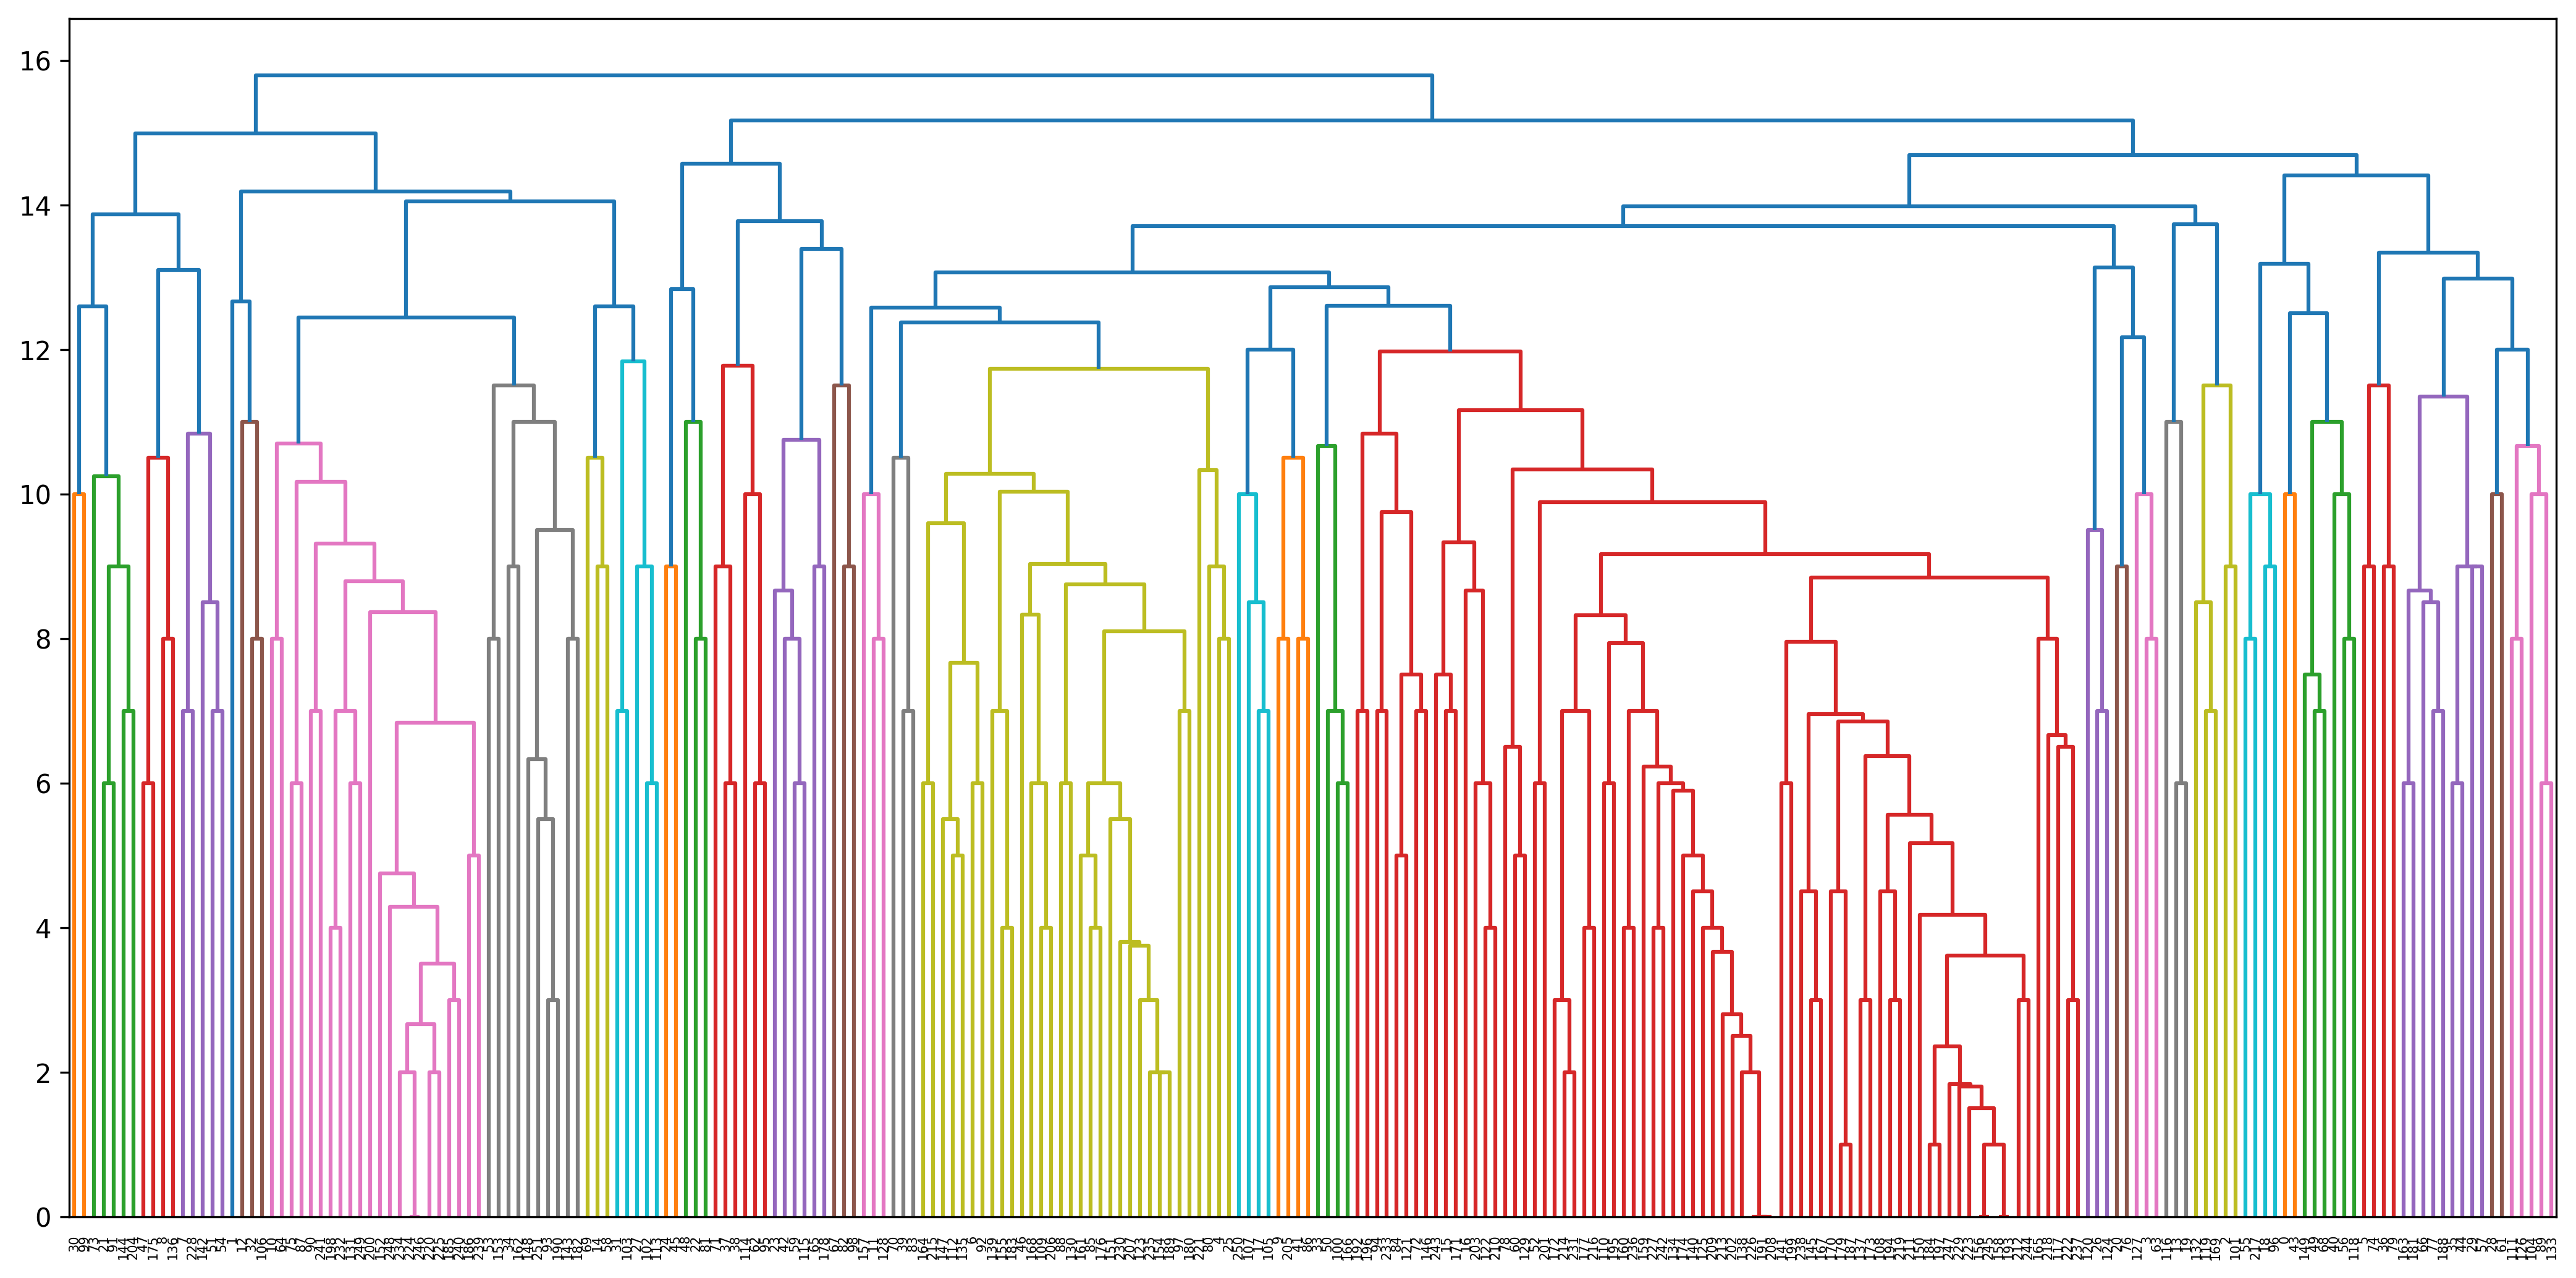
\includegraphics[width=\linewidth]{../Quantum-Annealing-for-solving-QUBO-Problems/test/Diagnostica_QALS/2/Decay_factor/ksp_3/lambda_650_dot_C/dendrogram_2000_1.png}
\caption{Agglomerative Clustering Dendogram}
\label{fig:AgglomerativeClustering-ksp3}
\end{figure}

\clearpage
\begin{figure}[H]
\centering
\begin{subfigure}{0.495\textwidth}
    \centering
    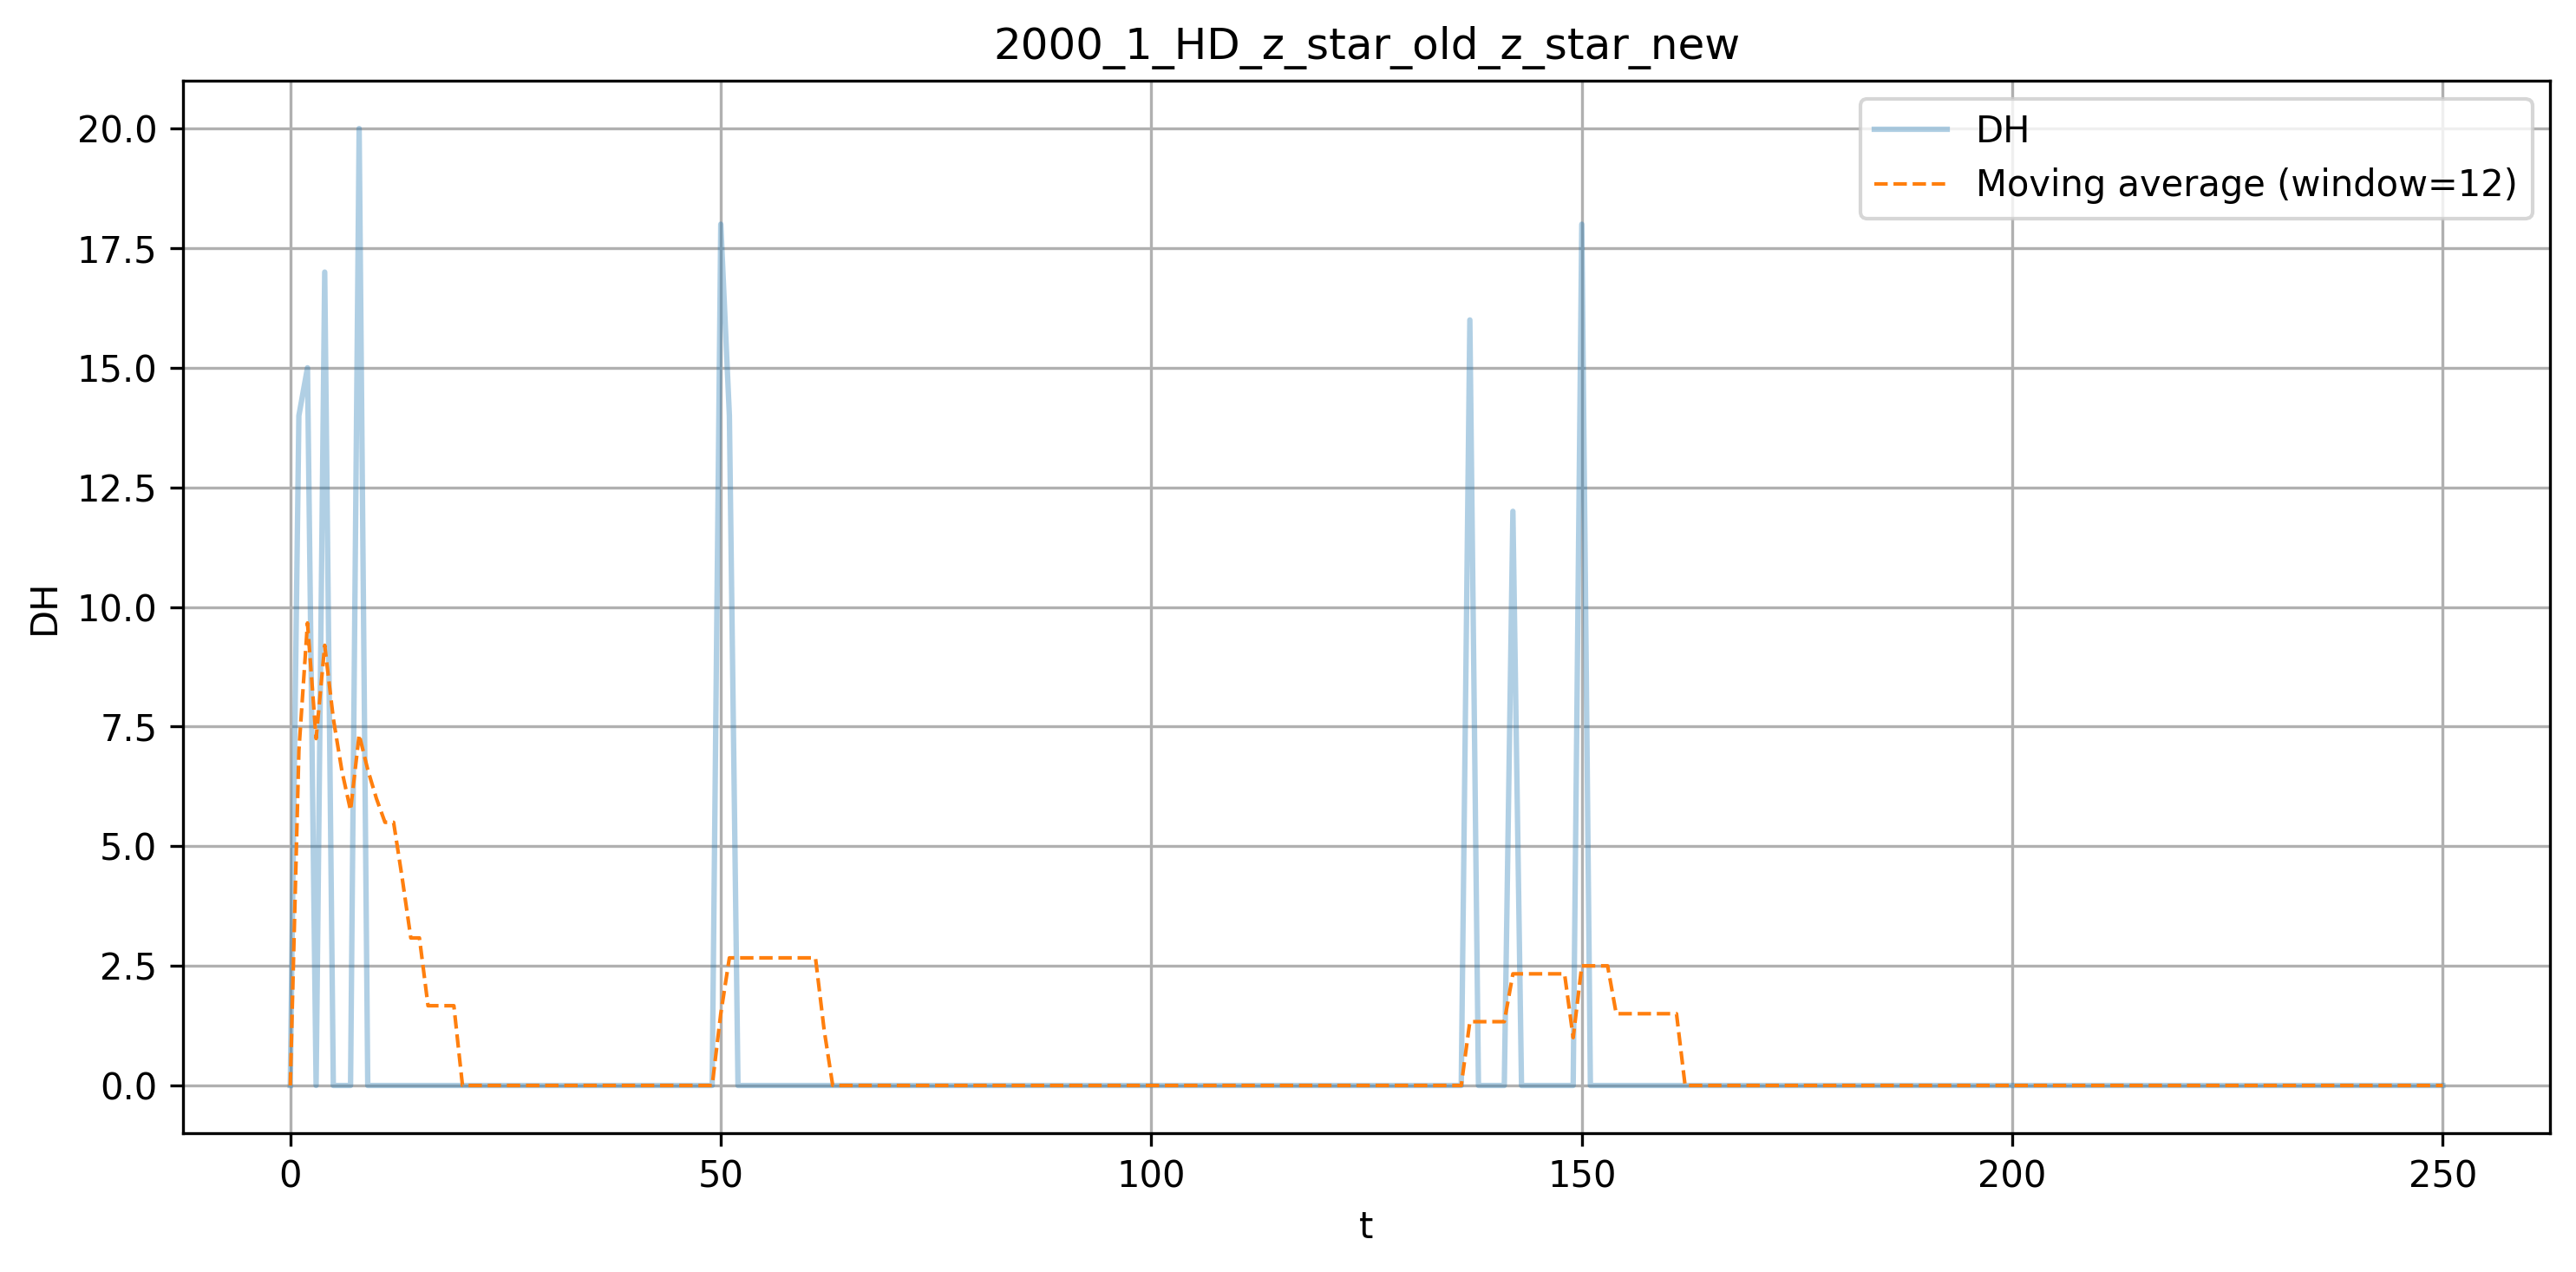
\includegraphics[width=\linewidth]{../Quantum-Annealing-for-solving-QUBO-Problems/test/Diagnostica_QALS/2/Decay_factor/ksp_3/lambda_div_3/2000_1_HD_z_star_old_z_star_new.png}
    \caption{\(d_H(z_\star^{old}, z_\star^{new})\) con \(\lambda_2\)}
    \label{fig:hd-zstarold-zstarnew-lambda2}
\end{subfigure}
\hfill
\begin{subfigure}{0.495\textwidth}
    \centering
    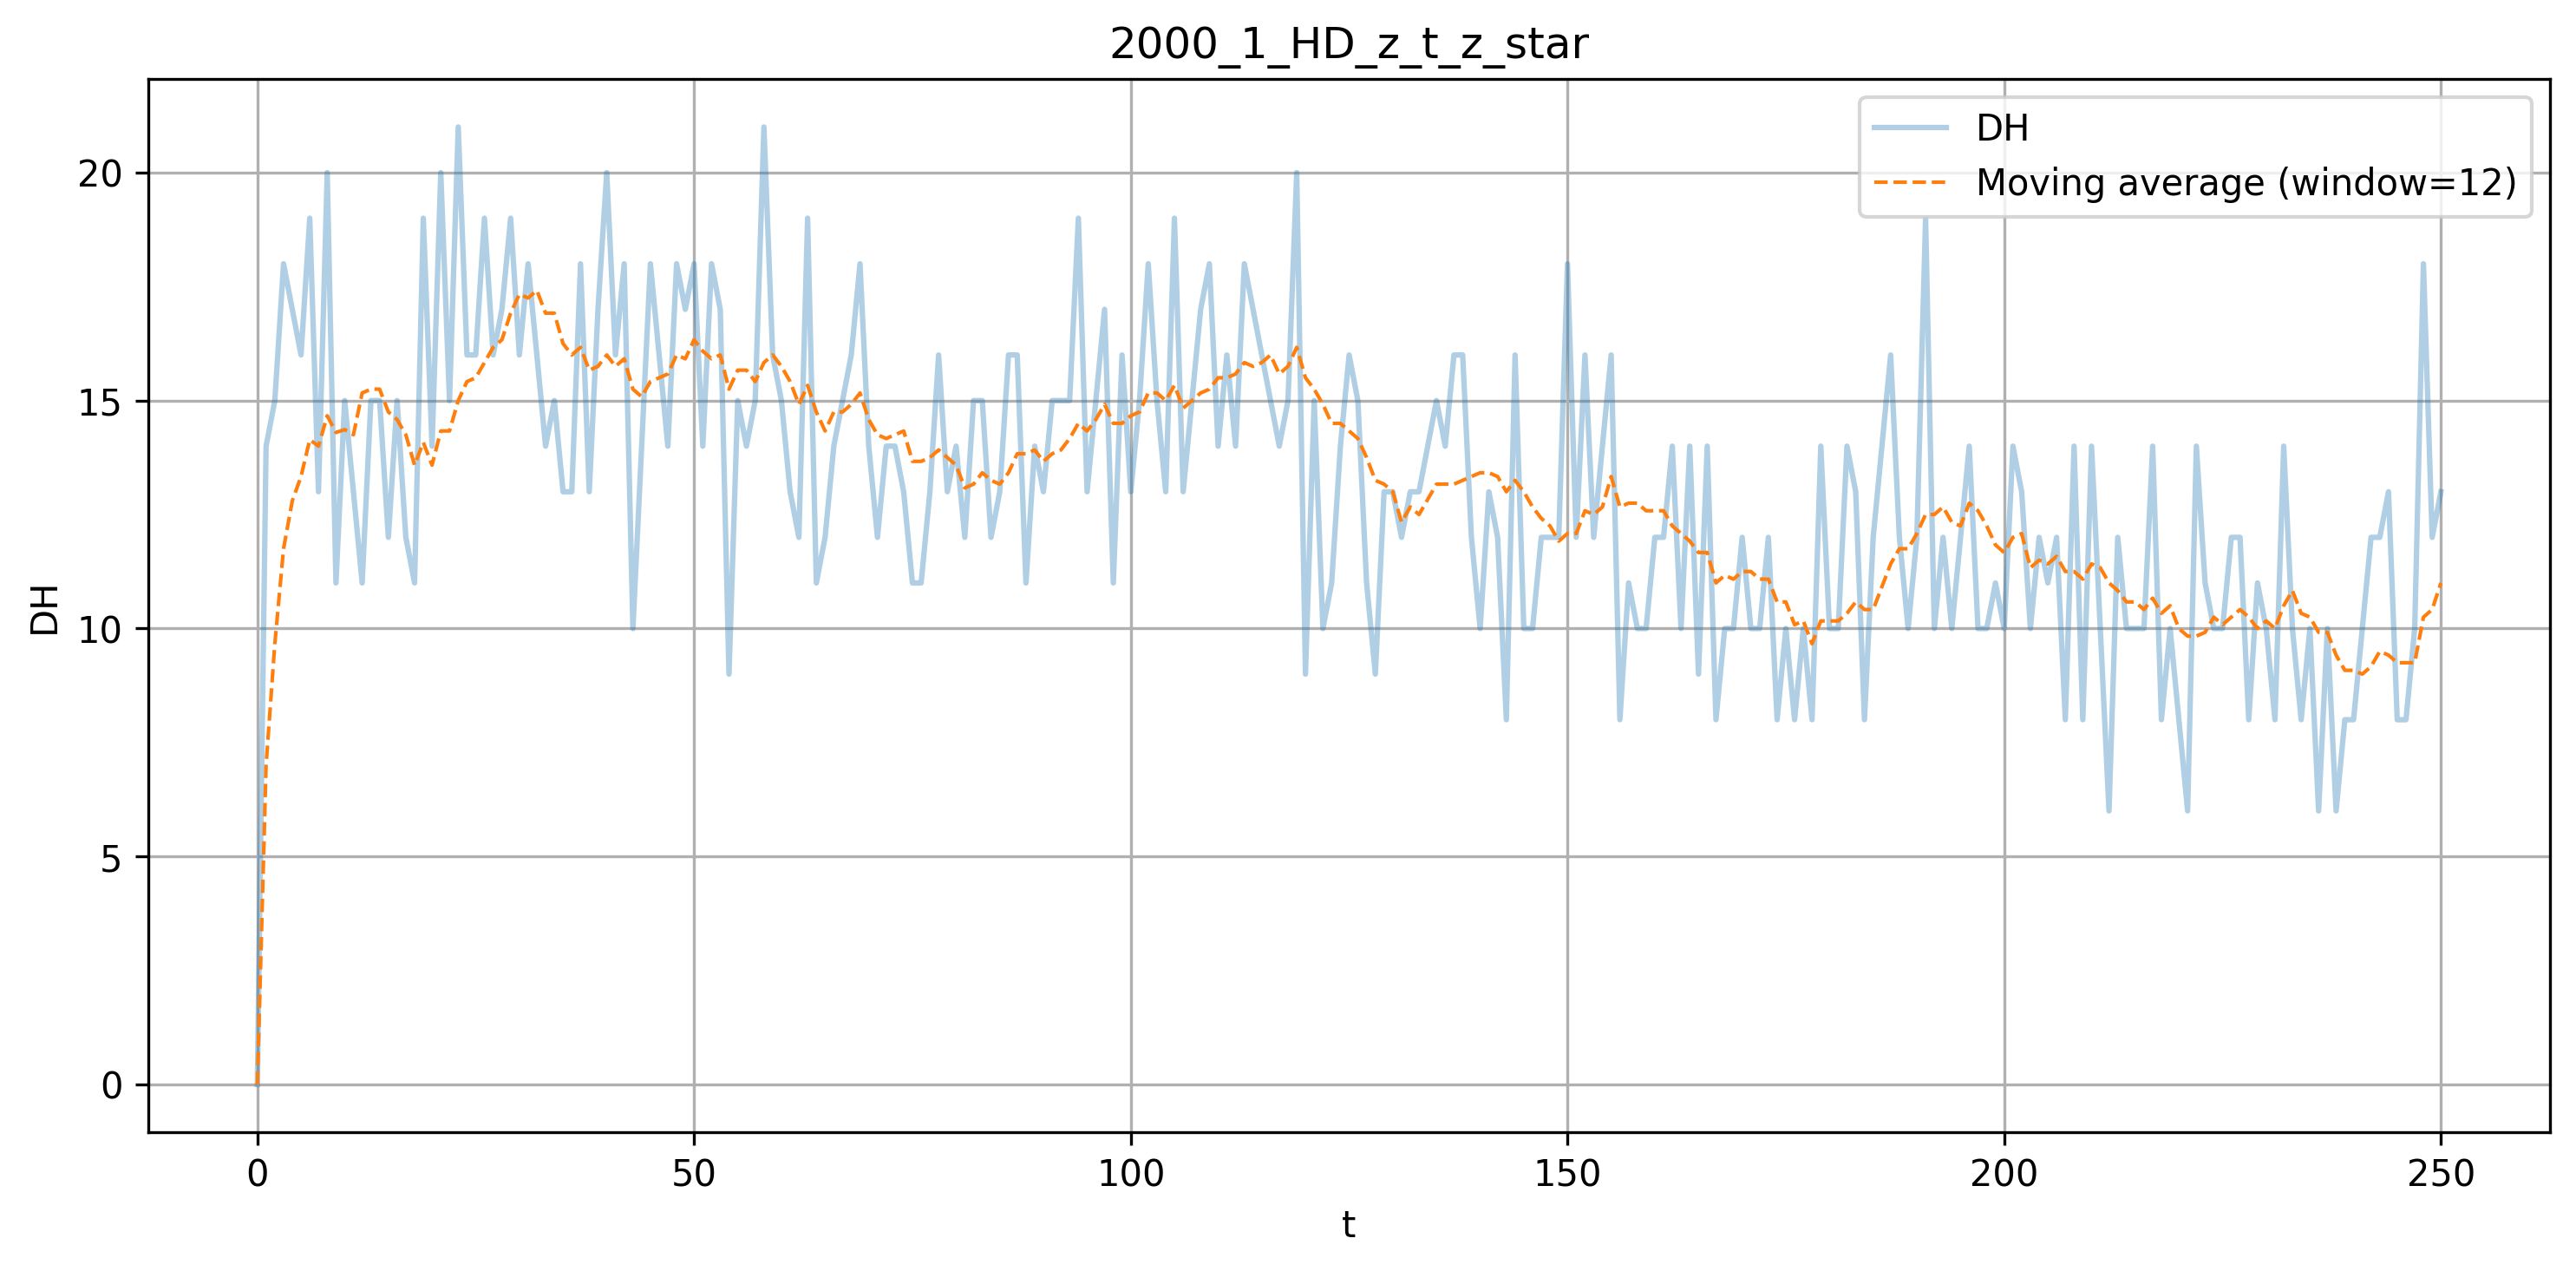
\includegraphics[width=\linewidth]{../Quantum-Annealing-for-solving-QUBO-Problems/test/Diagnostica_QALS/2/Decay_factor/ksp_3/lambda_div_3/2000_1_HD_z_t_z_star.png}
    \caption{\(d_H(z_t, z_\star)\) con \(\lambda_2\)}
    \label{fig:hd-zt-zstar-lambda2}
\end{subfigure}

\vspace{0.35cm}

\begin{subfigure}{0.495\textwidth}
    \centering
    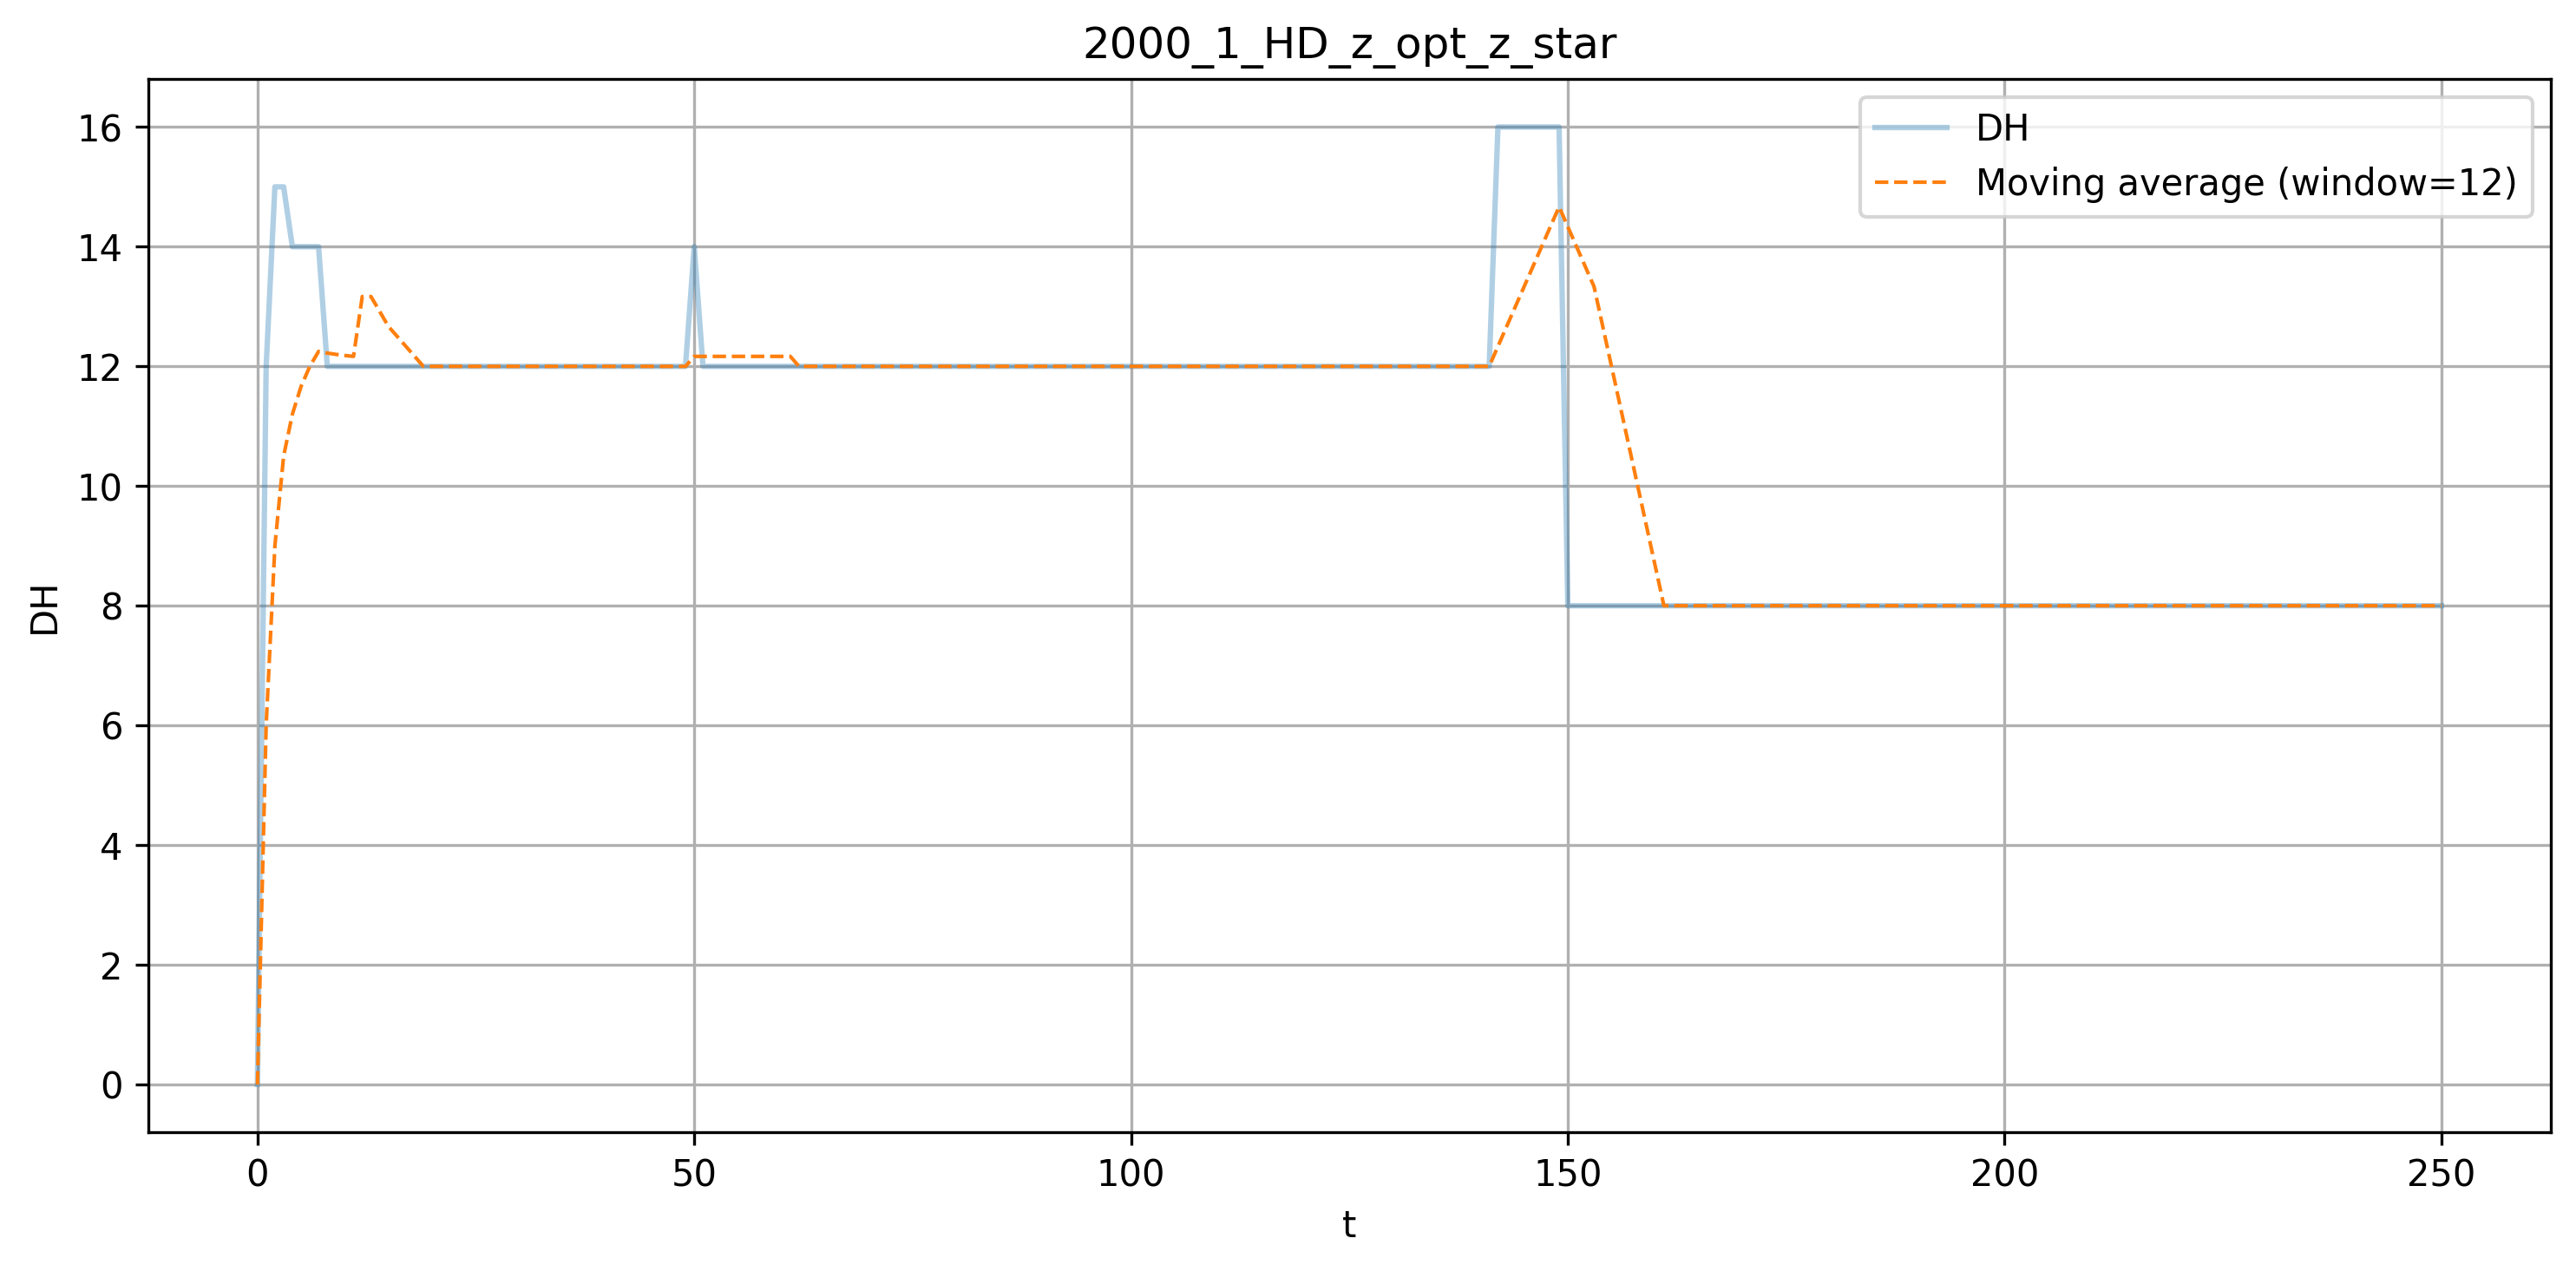
\includegraphics[width=\linewidth]{../Quantum-Annealing-for-solving-QUBO-Problems/test/Diagnostica_QALS/2/Decay_factor/ksp_3/lambda_div_3/2000_1_HD_z_opt_z_star.png}
    \caption{\(d_H(z_{opt}, z_\star)\) con \(\lambda_2\)}
    \label{fig:hd-zopt-zstar-lambda2}
\end{subfigure}
\hfill
\begin{subfigure}{0.495\textwidth}
    \centering
    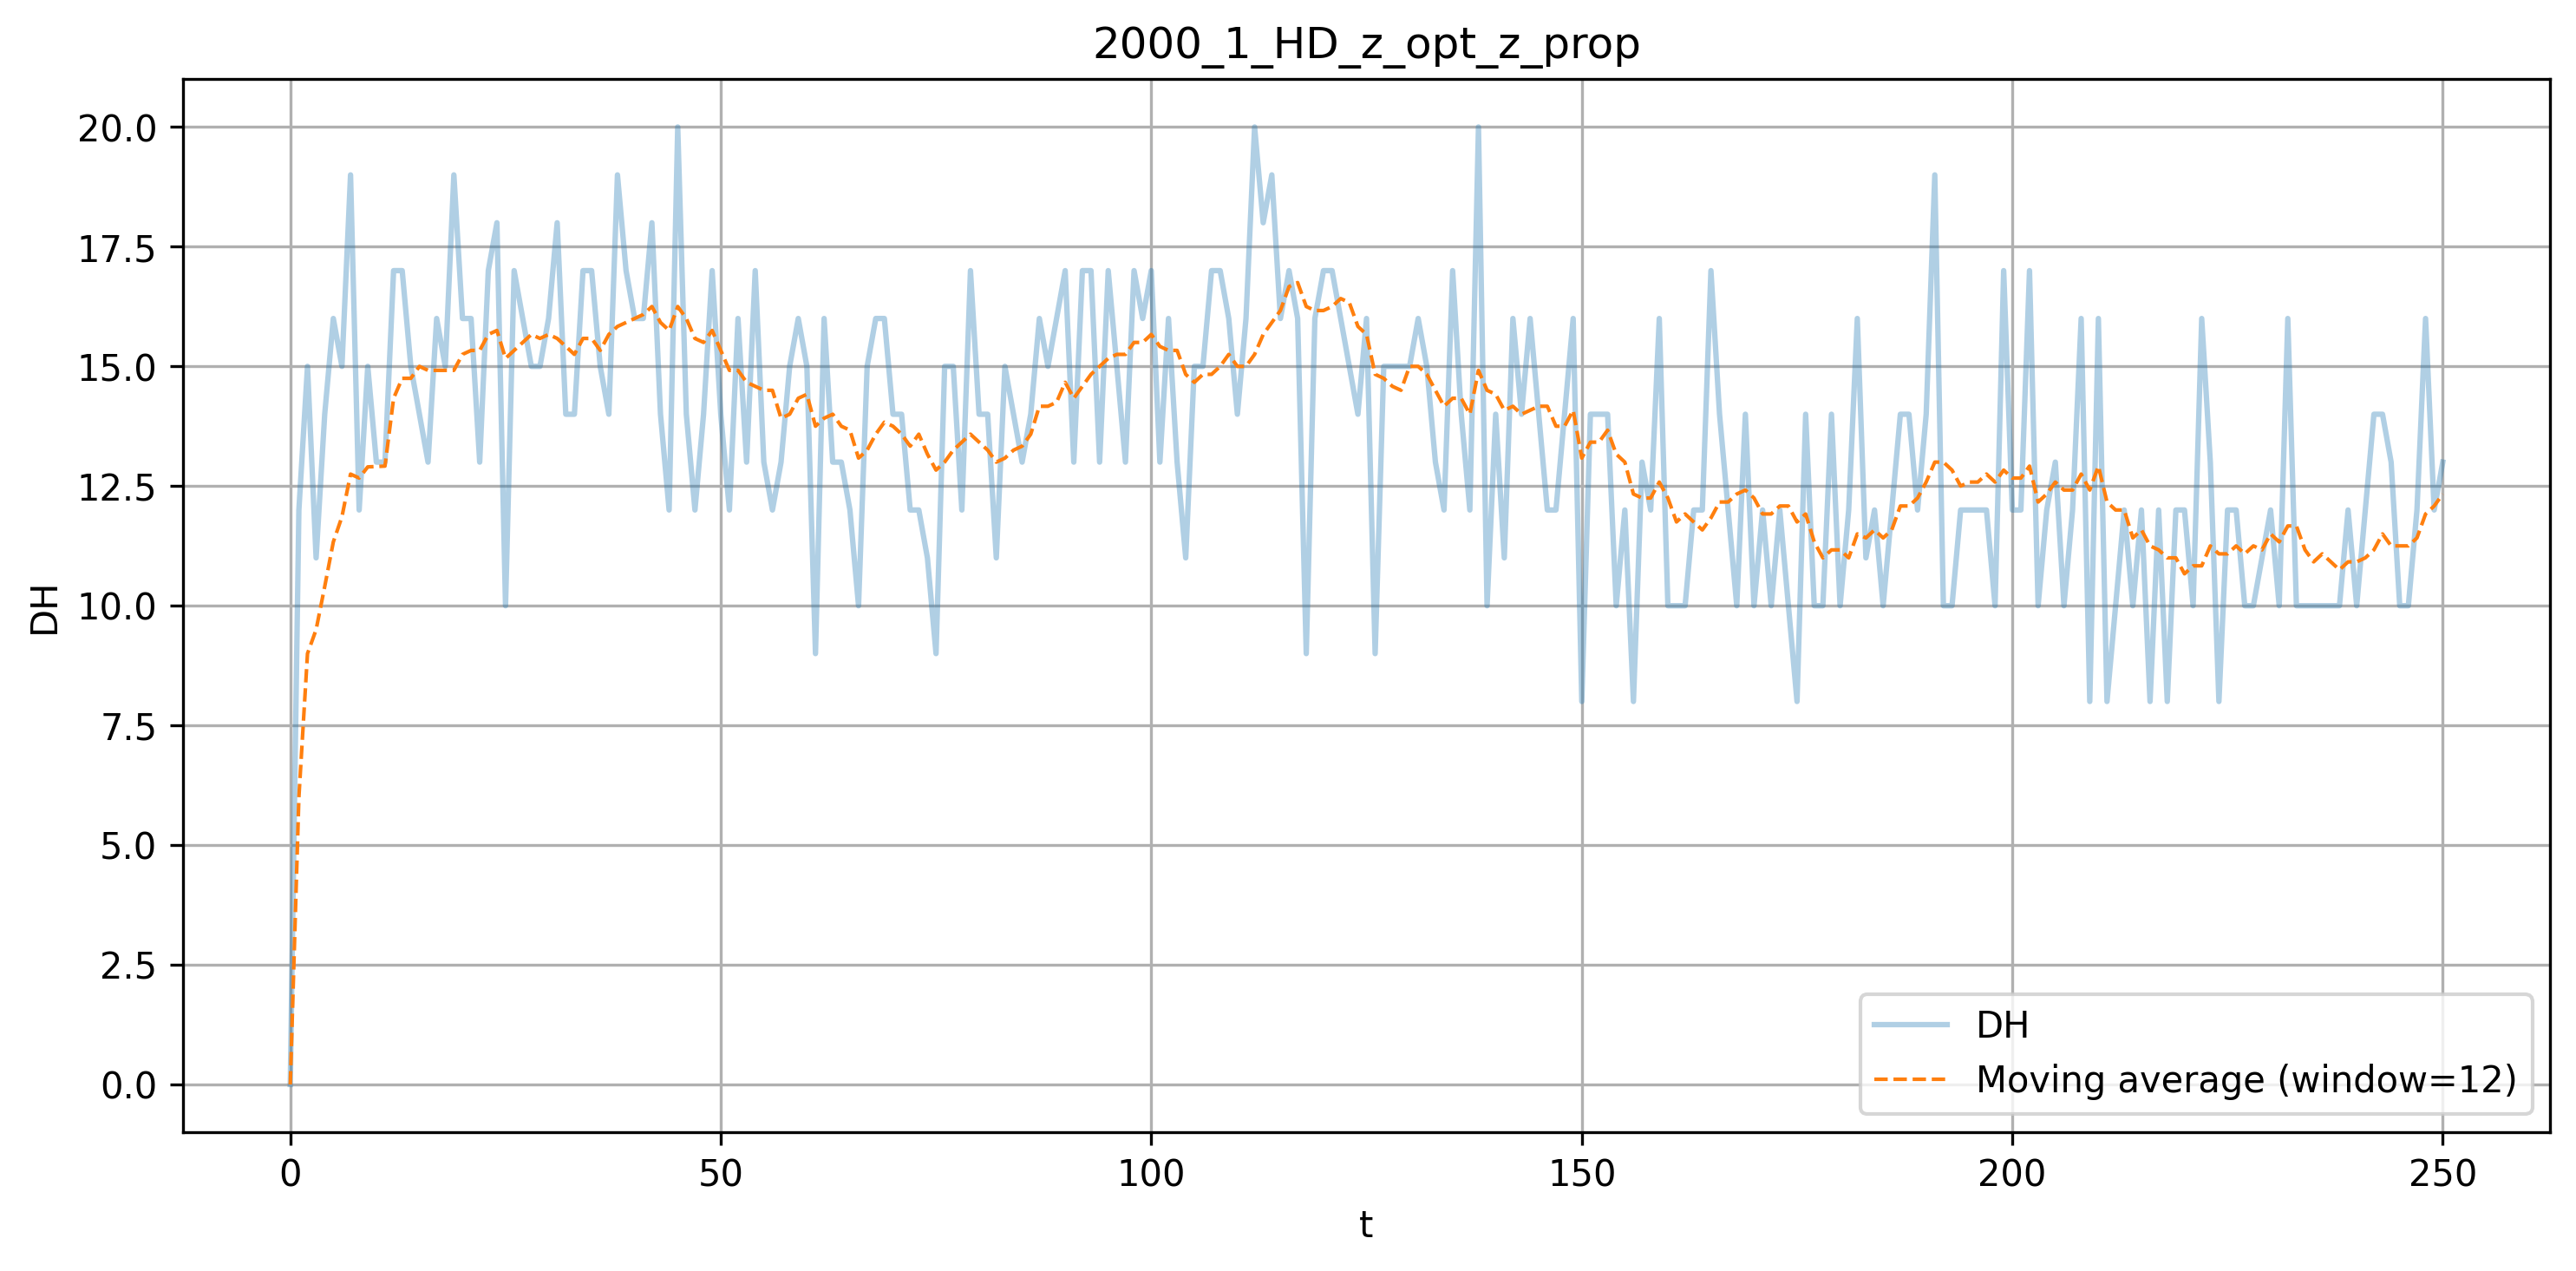
\includegraphics[width=\linewidth]{../Quantum-Annealing-for-solving-QUBO-Problems/test/Diagnostica_QALS/2/Decay_factor/ksp_3/lambda_div_3/2000_1_HD_z_opt_z_prop.png}
    \caption{\(d_H(z_{opt}, z_t)\) con \(\lambda_2\)}
    \label{fig:hd-zopt-zt-lambda2}
\end{subfigure}

\vspace{0.35cm}

\begin{subfigure}{0.495\textwidth}
    \centering
    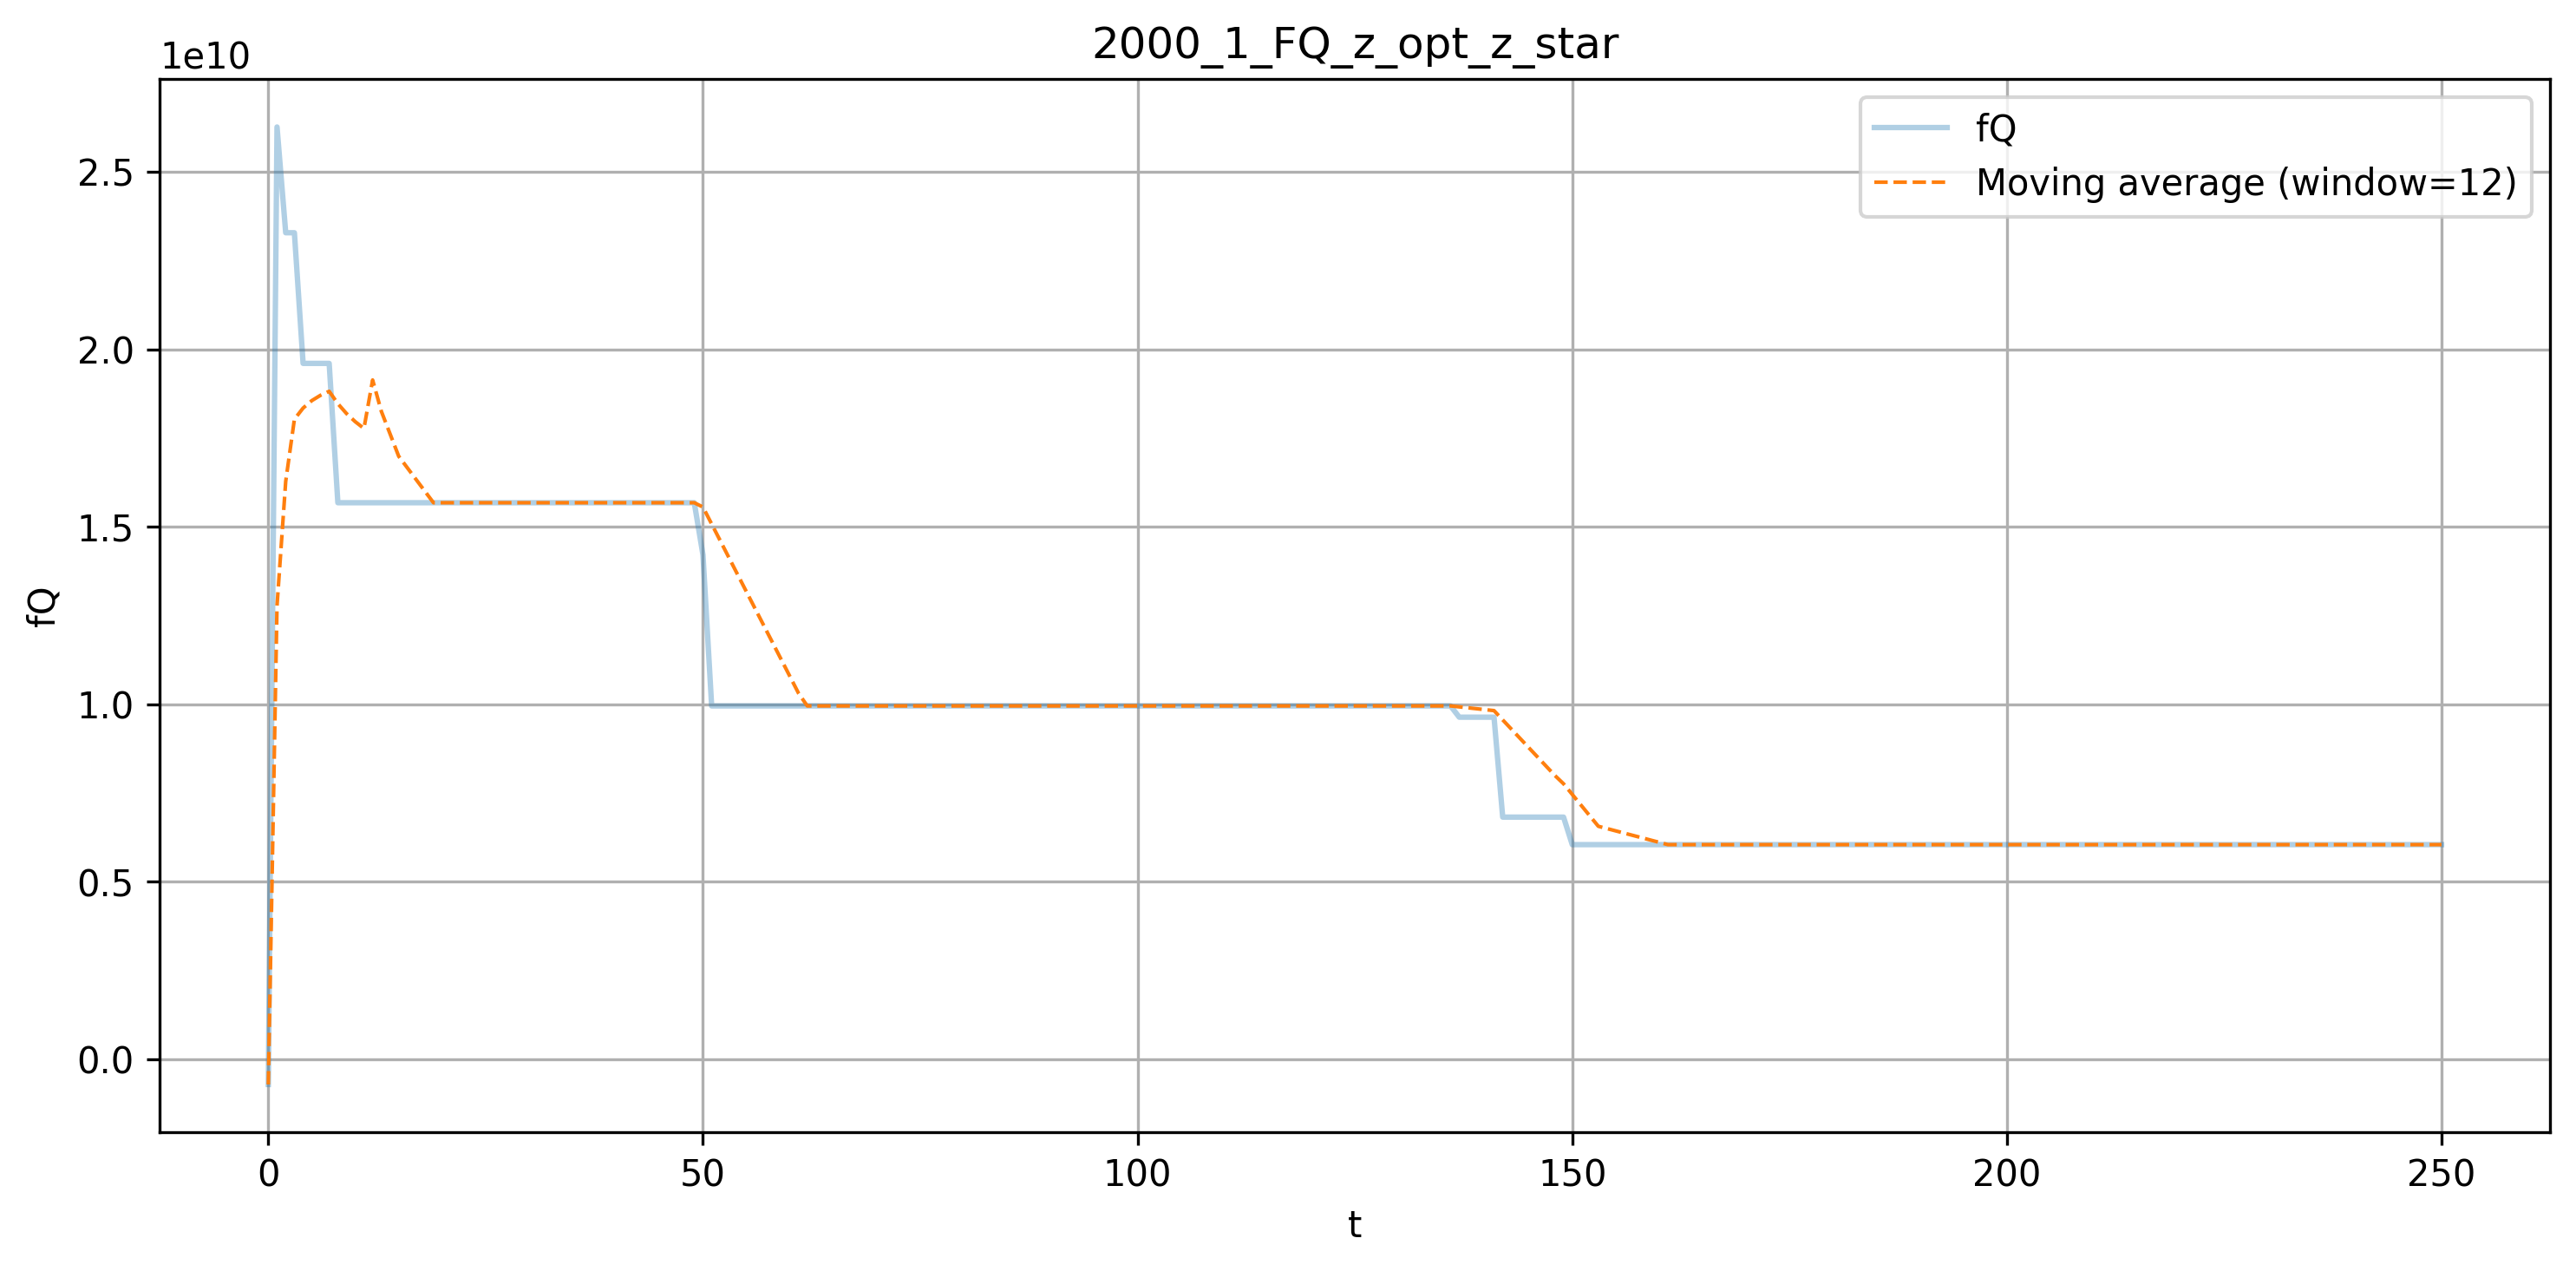
\includegraphics[width=\linewidth]{../Quantum-Annealing-for-solving-QUBO-Problems/test/Diagnostica_QALS/2/Decay_factor/ksp_3/lambda_div_3/2000_1_FQ_z_opt_z_star.png}
    \caption{\(f_Q(z_\star)\) con \(\lambda_2\)}
    \label{fig:fQ-zstar-lambda2}
\end{subfigure}
\hfill
\begin{subfigure}{0.495\textwidth}
    \centering
    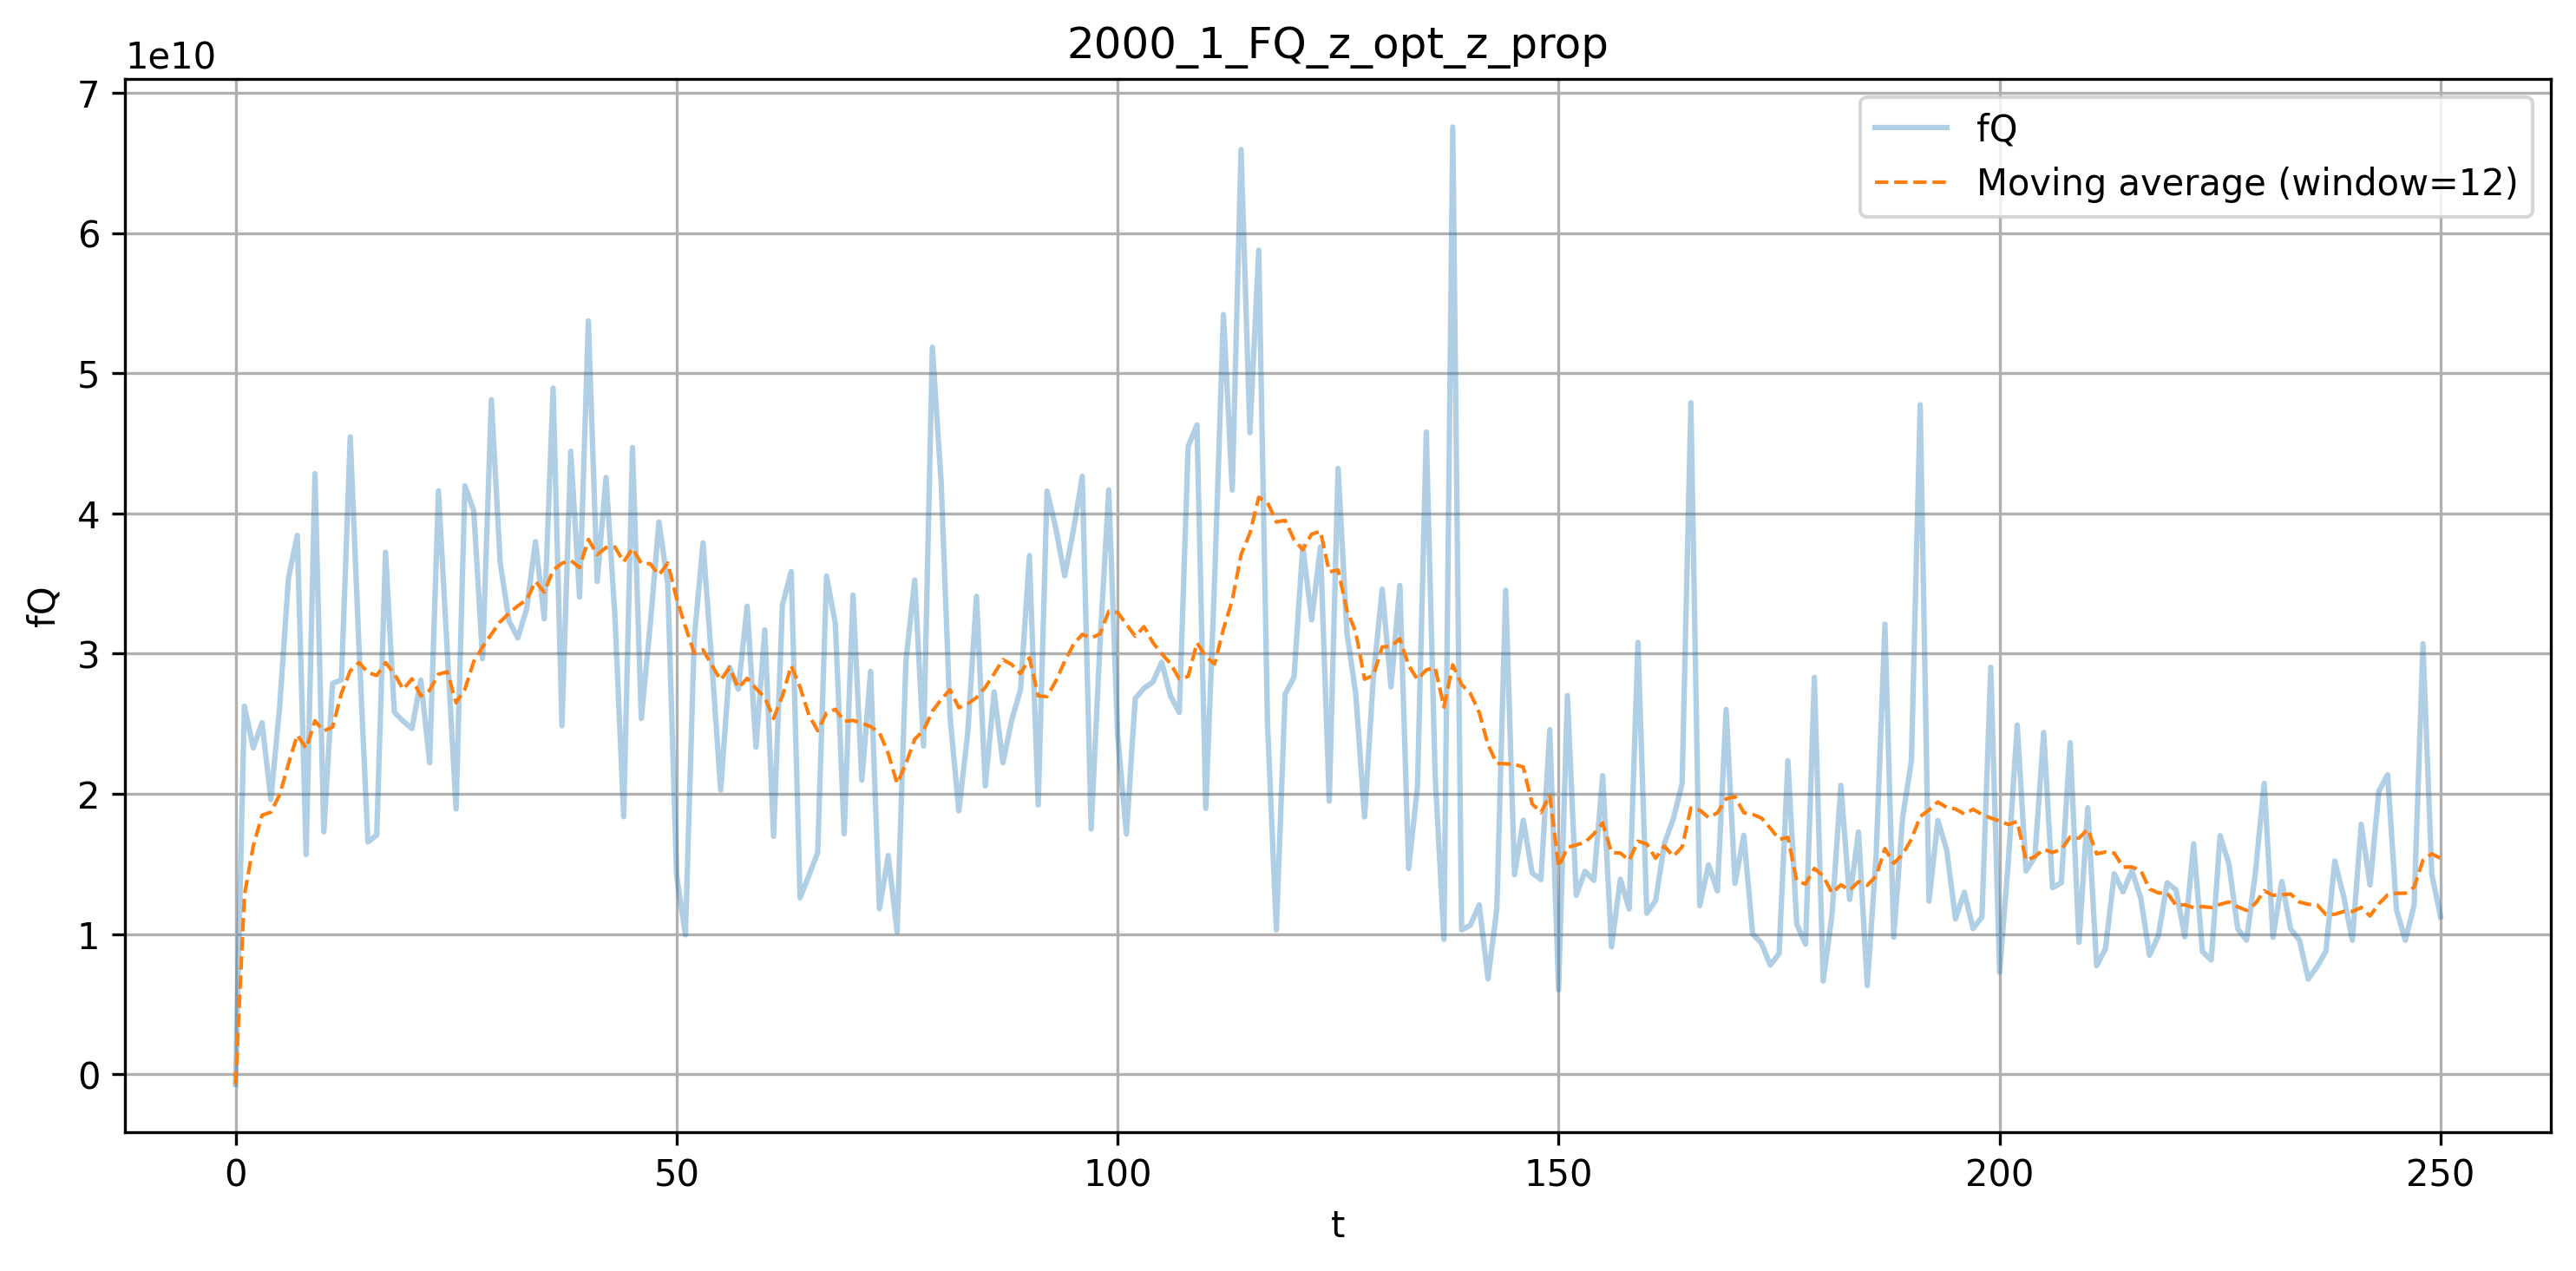
\includegraphics[width=\linewidth]{../Quantum-Annealing-for-solving-QUBO-Problems/test/Diagnostica_QALS/2/Decay_factor/ksp_3/lambda_div_3/2000_1_FQ_z_opt_z_prop.png}
    \caption{\(f_Q(z_t)\) con \(\lambda_2\)}
    \label{fig:fQ-zt-lambda2}
\end{subfigure}
\label{fig:confronto-hamming-ksp32}
\end{figure}

\begin{figure}[H]
\centering
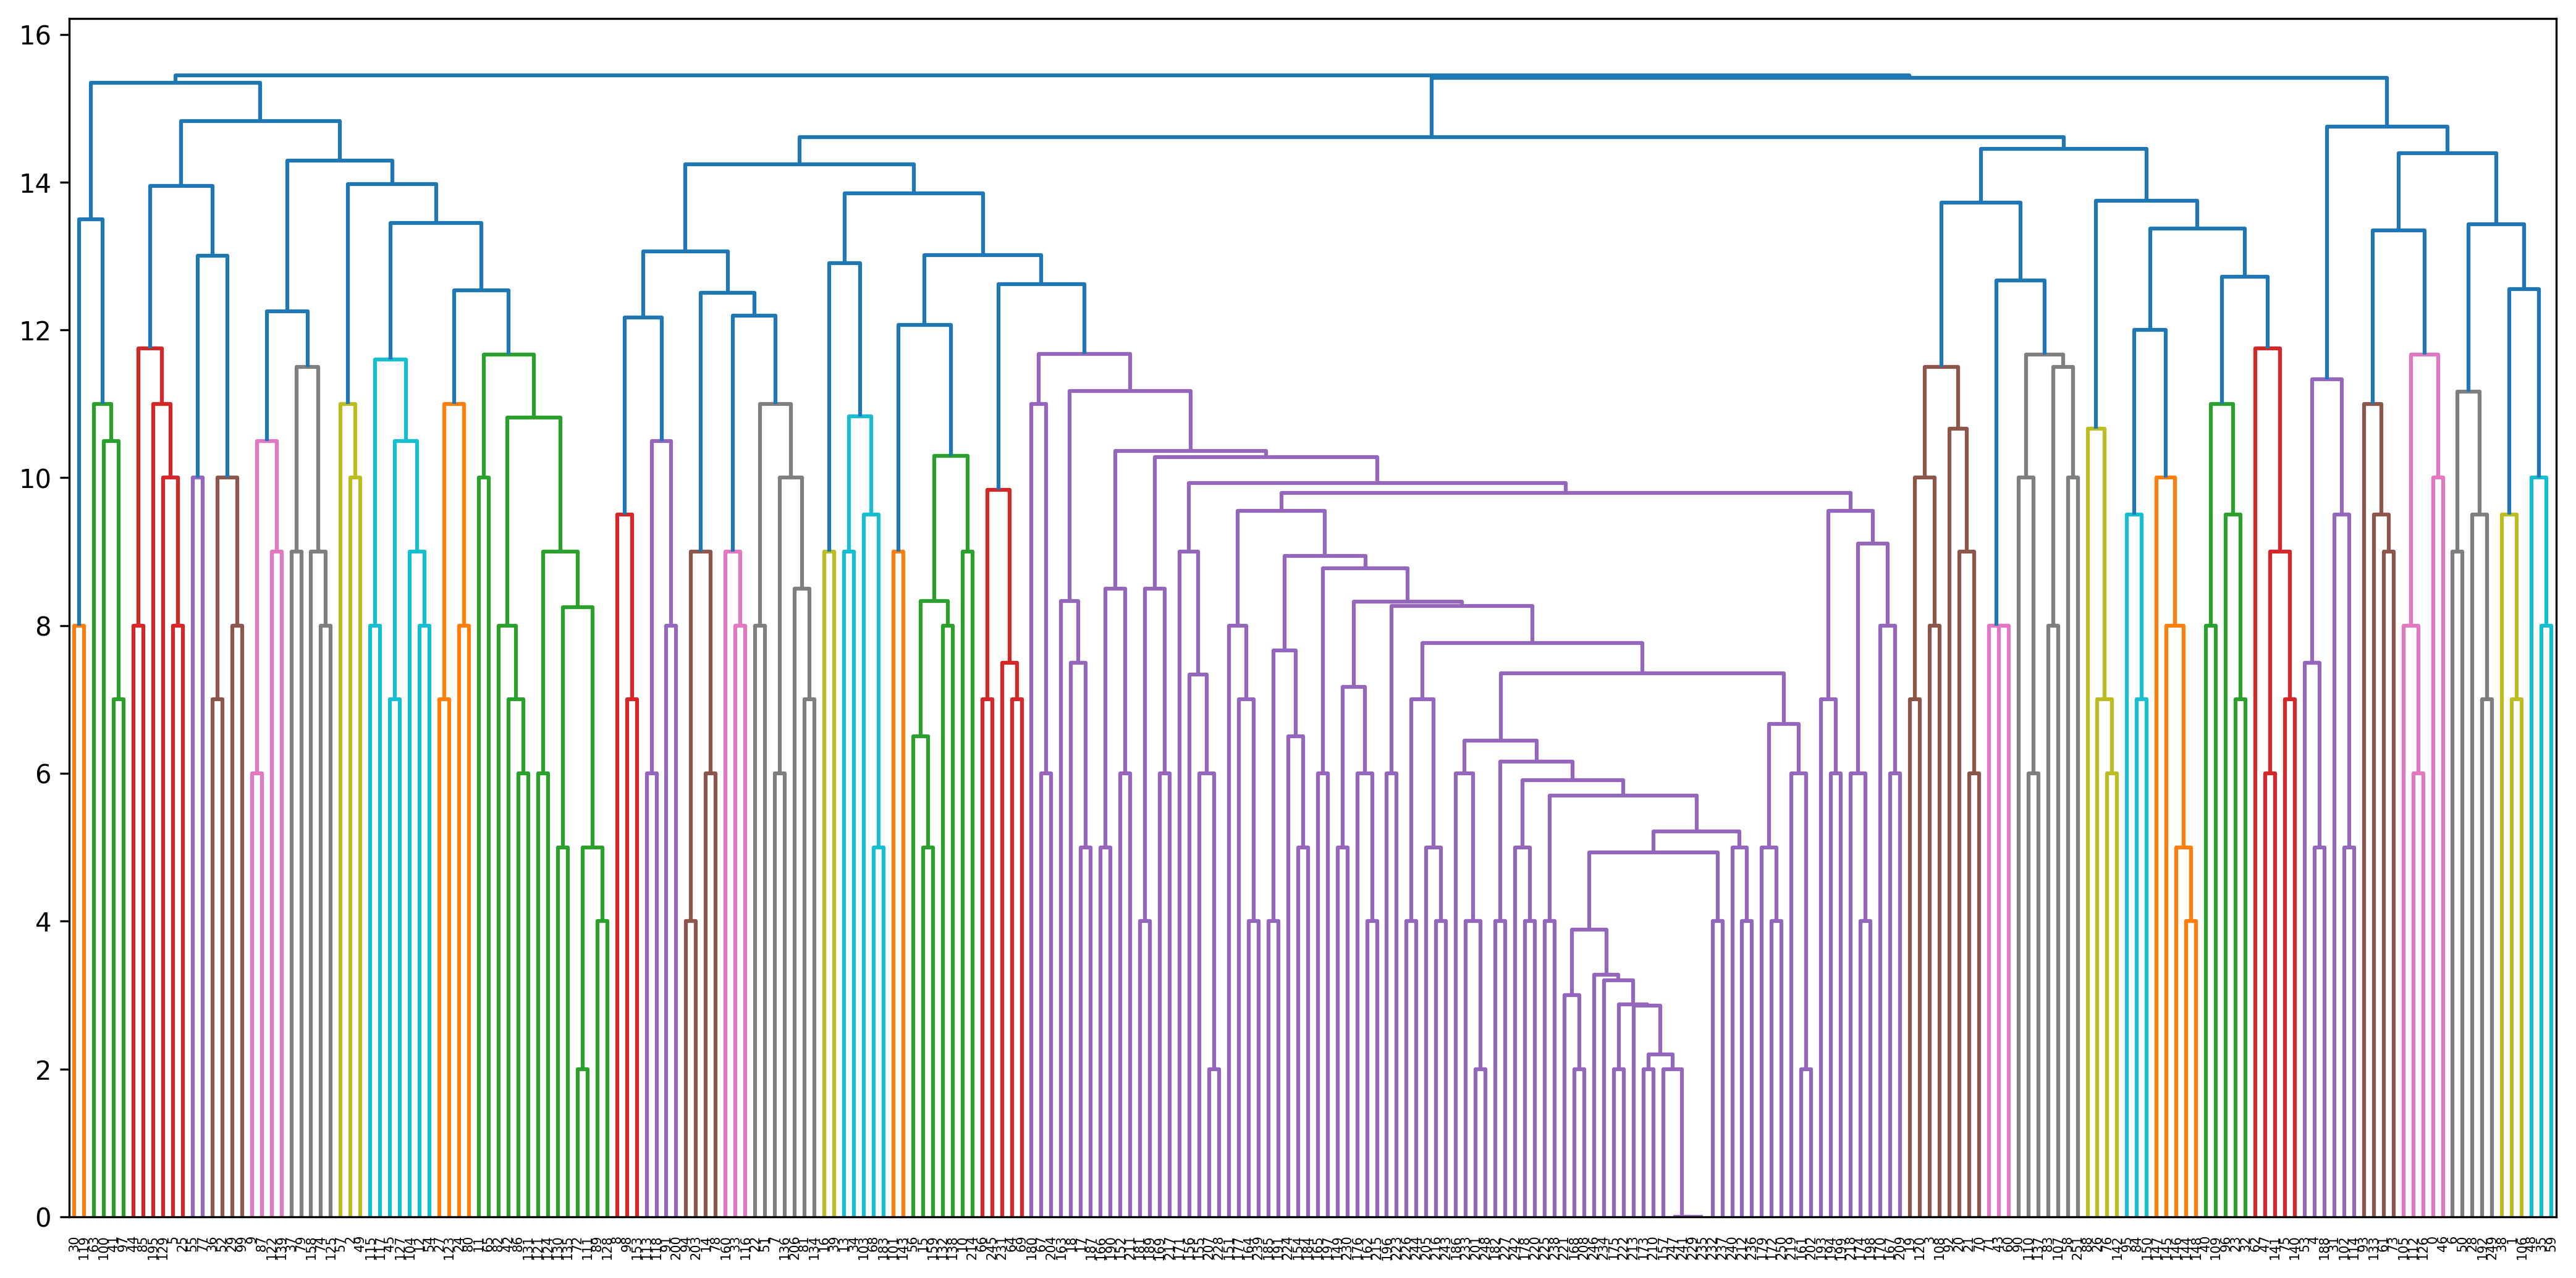
\includegraphics[width=\linewidth]{../Quantum-Annealing-for-solving-QUBO-Problems/test/Diagnostica_QALS/2/Decay_factor/ksp_3/lambda_div_3/dendrogram_2000_1.png}
\caption{Agglomerative Clustering Dendogram}
\label{fig:AgglomerativeClustering-ksp3}
\end{figure}

\clearpage
\subsection{ksp\_2}

\begin{table}[h]
\centering
\begin{tabular}{lcc}
\hline
\textbf{Metrica} & \(\lambda_1\) & \(\lambda_2\) \\
\hline
Numero cluster & 49 & 50 \\
Dimensione cluster massimo & 102 & 105 \\
Cluster z best & 31 & 20 \\
Single clusters & 11 & 5 \\
\(f_Q\) medoid & 7997845.02 & 967718038887.67 \\
Profit medoid & 17741 & 14979 \\
Weight medoid & 14107 & 10802 \\
\hline
\(f_Q\) Min Found QALS & 2232153.7 & 417407498726.0 \\
Profit Found QALS & 10988 & 13194 \\
Weight Found QALS & 7986 & 7482 \\
\hline
\(f_Q\) Min Found NO QALS &	-54748.31 & -10200710054.33 \\
Profit Found NO QALS & 7740 & 5874 \\
Weight Found NO QALS & 978 & 1001 \\
\hline
\end{tabular}

\caption{Confronto dei risultati ottenuti con QALS e senza QALS.}
\label{tab:confronto-qals-noqals}
\end{table}

\begin{figure}[H]
\centering
\begin{subfigure}{0.495\textwidth}
    \centering
    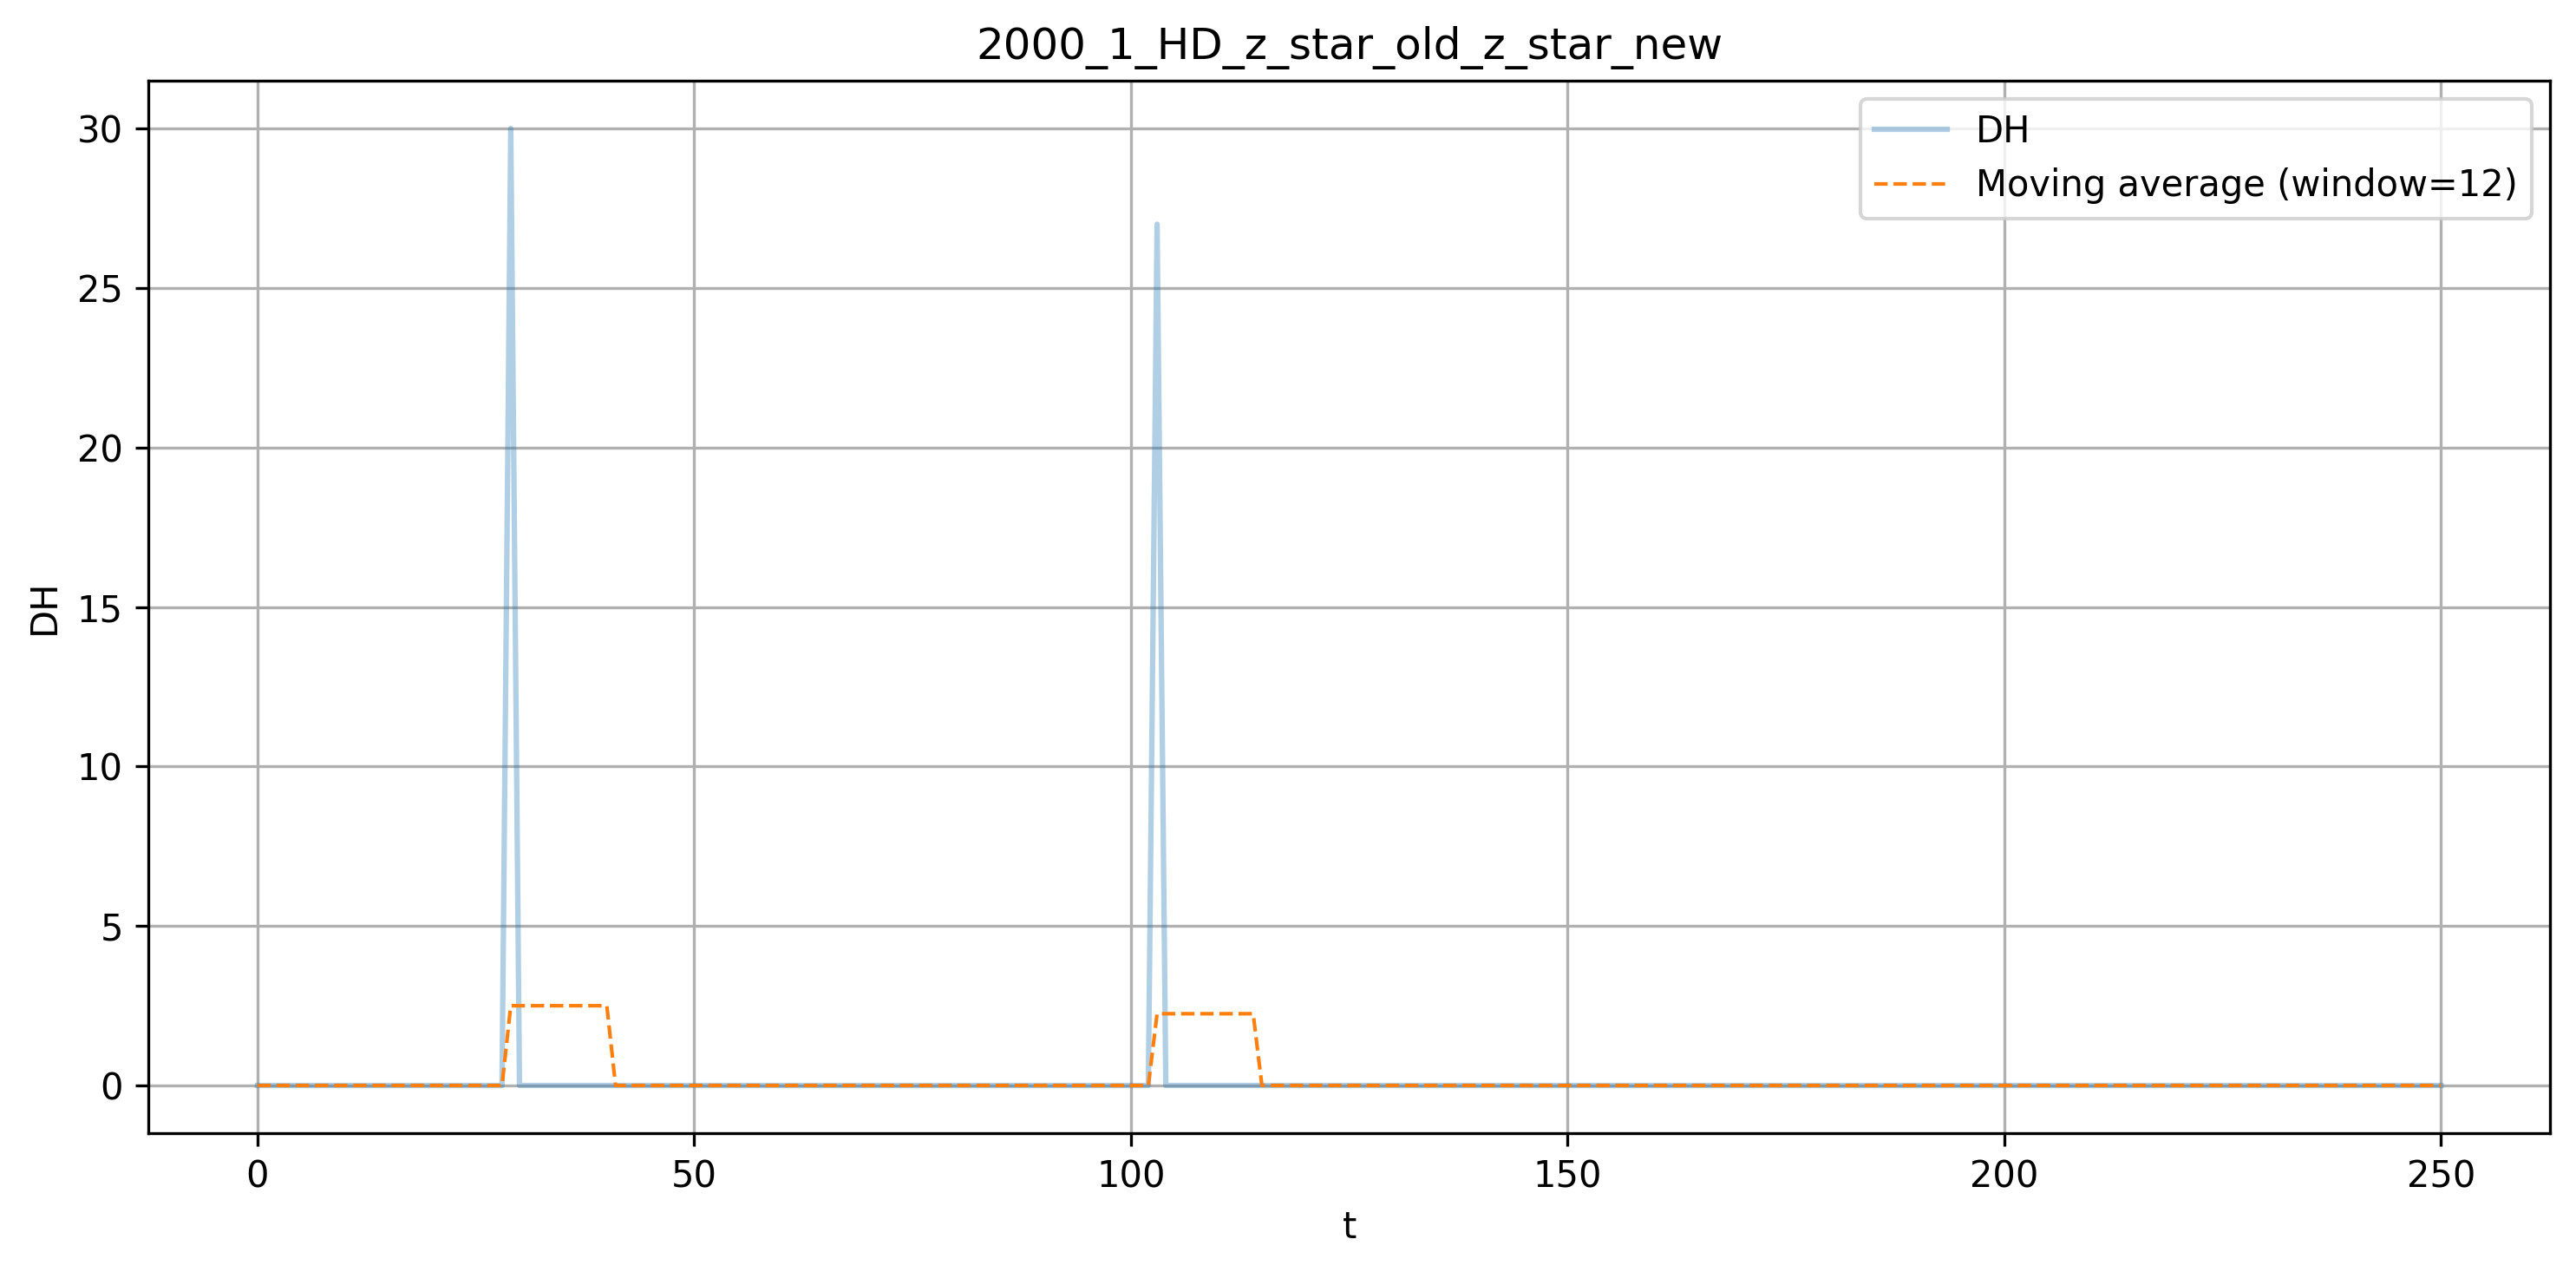
\includegraphics[width=\linewidth]{../Quantum-Annealing-for-solving-QUBO-Problems/test/Diagnostica_QALS/2/Decay_factor/ksp_2/lambda_650_dot_C/2000_1_HD_z_star_old_z_star_new.png}
    \caption{\(d_H(z_\star^{old}, z_\star^{new})\) con \(\lambda_1\)}
    \label{fig:hd-zstarold-zstarnew-lambda1}
\end{subfigure}
\hfill
\begin{subfigure}{0.495\textwidth}
    \centering
    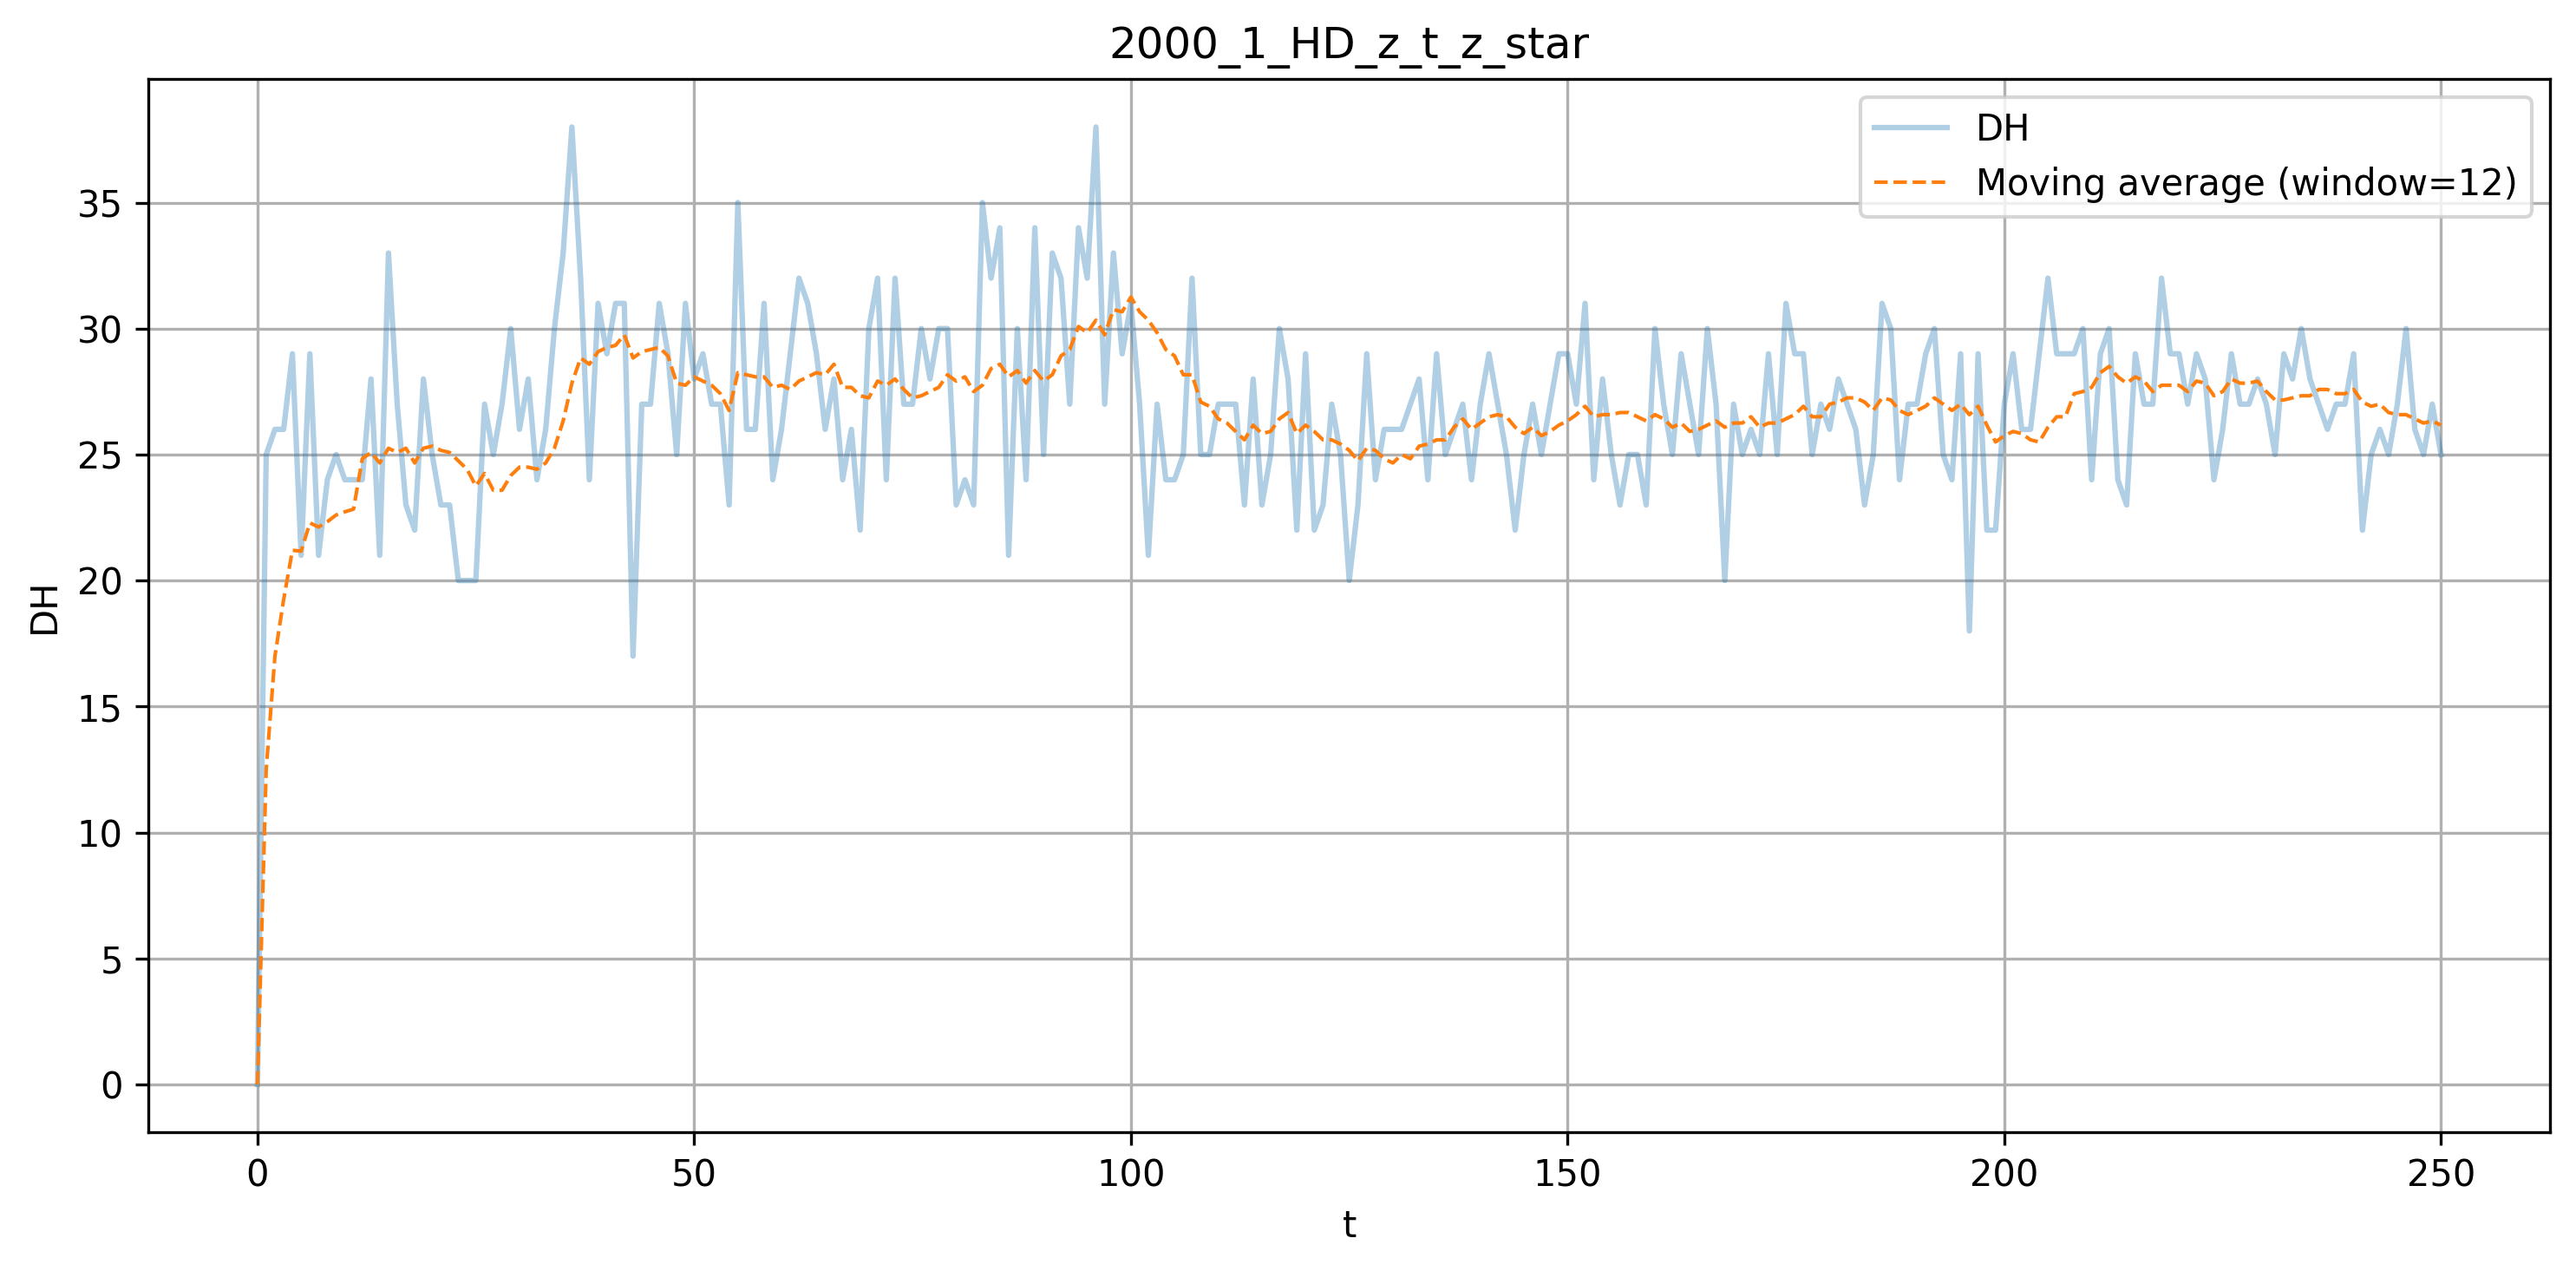
\includegraphics[width=\linewidth]{../Quantum-Annealing-for-solving-QUBO-Problems/test/Diagnostica_QALS/2/Decay_factor/ksp_2/lambda_650_dot_C/2000_1_HD_z_t_z_star.png}
    \caption{\(d_H(z_t, z_\star)\) con \(\lambda_1\)}
    \label{fig:hd-zt-zstar-lambda1}
\end{subfigure}

\vspace{0.35cm}

\begin{subfigure}{0.495\textwidth}
    \centering
    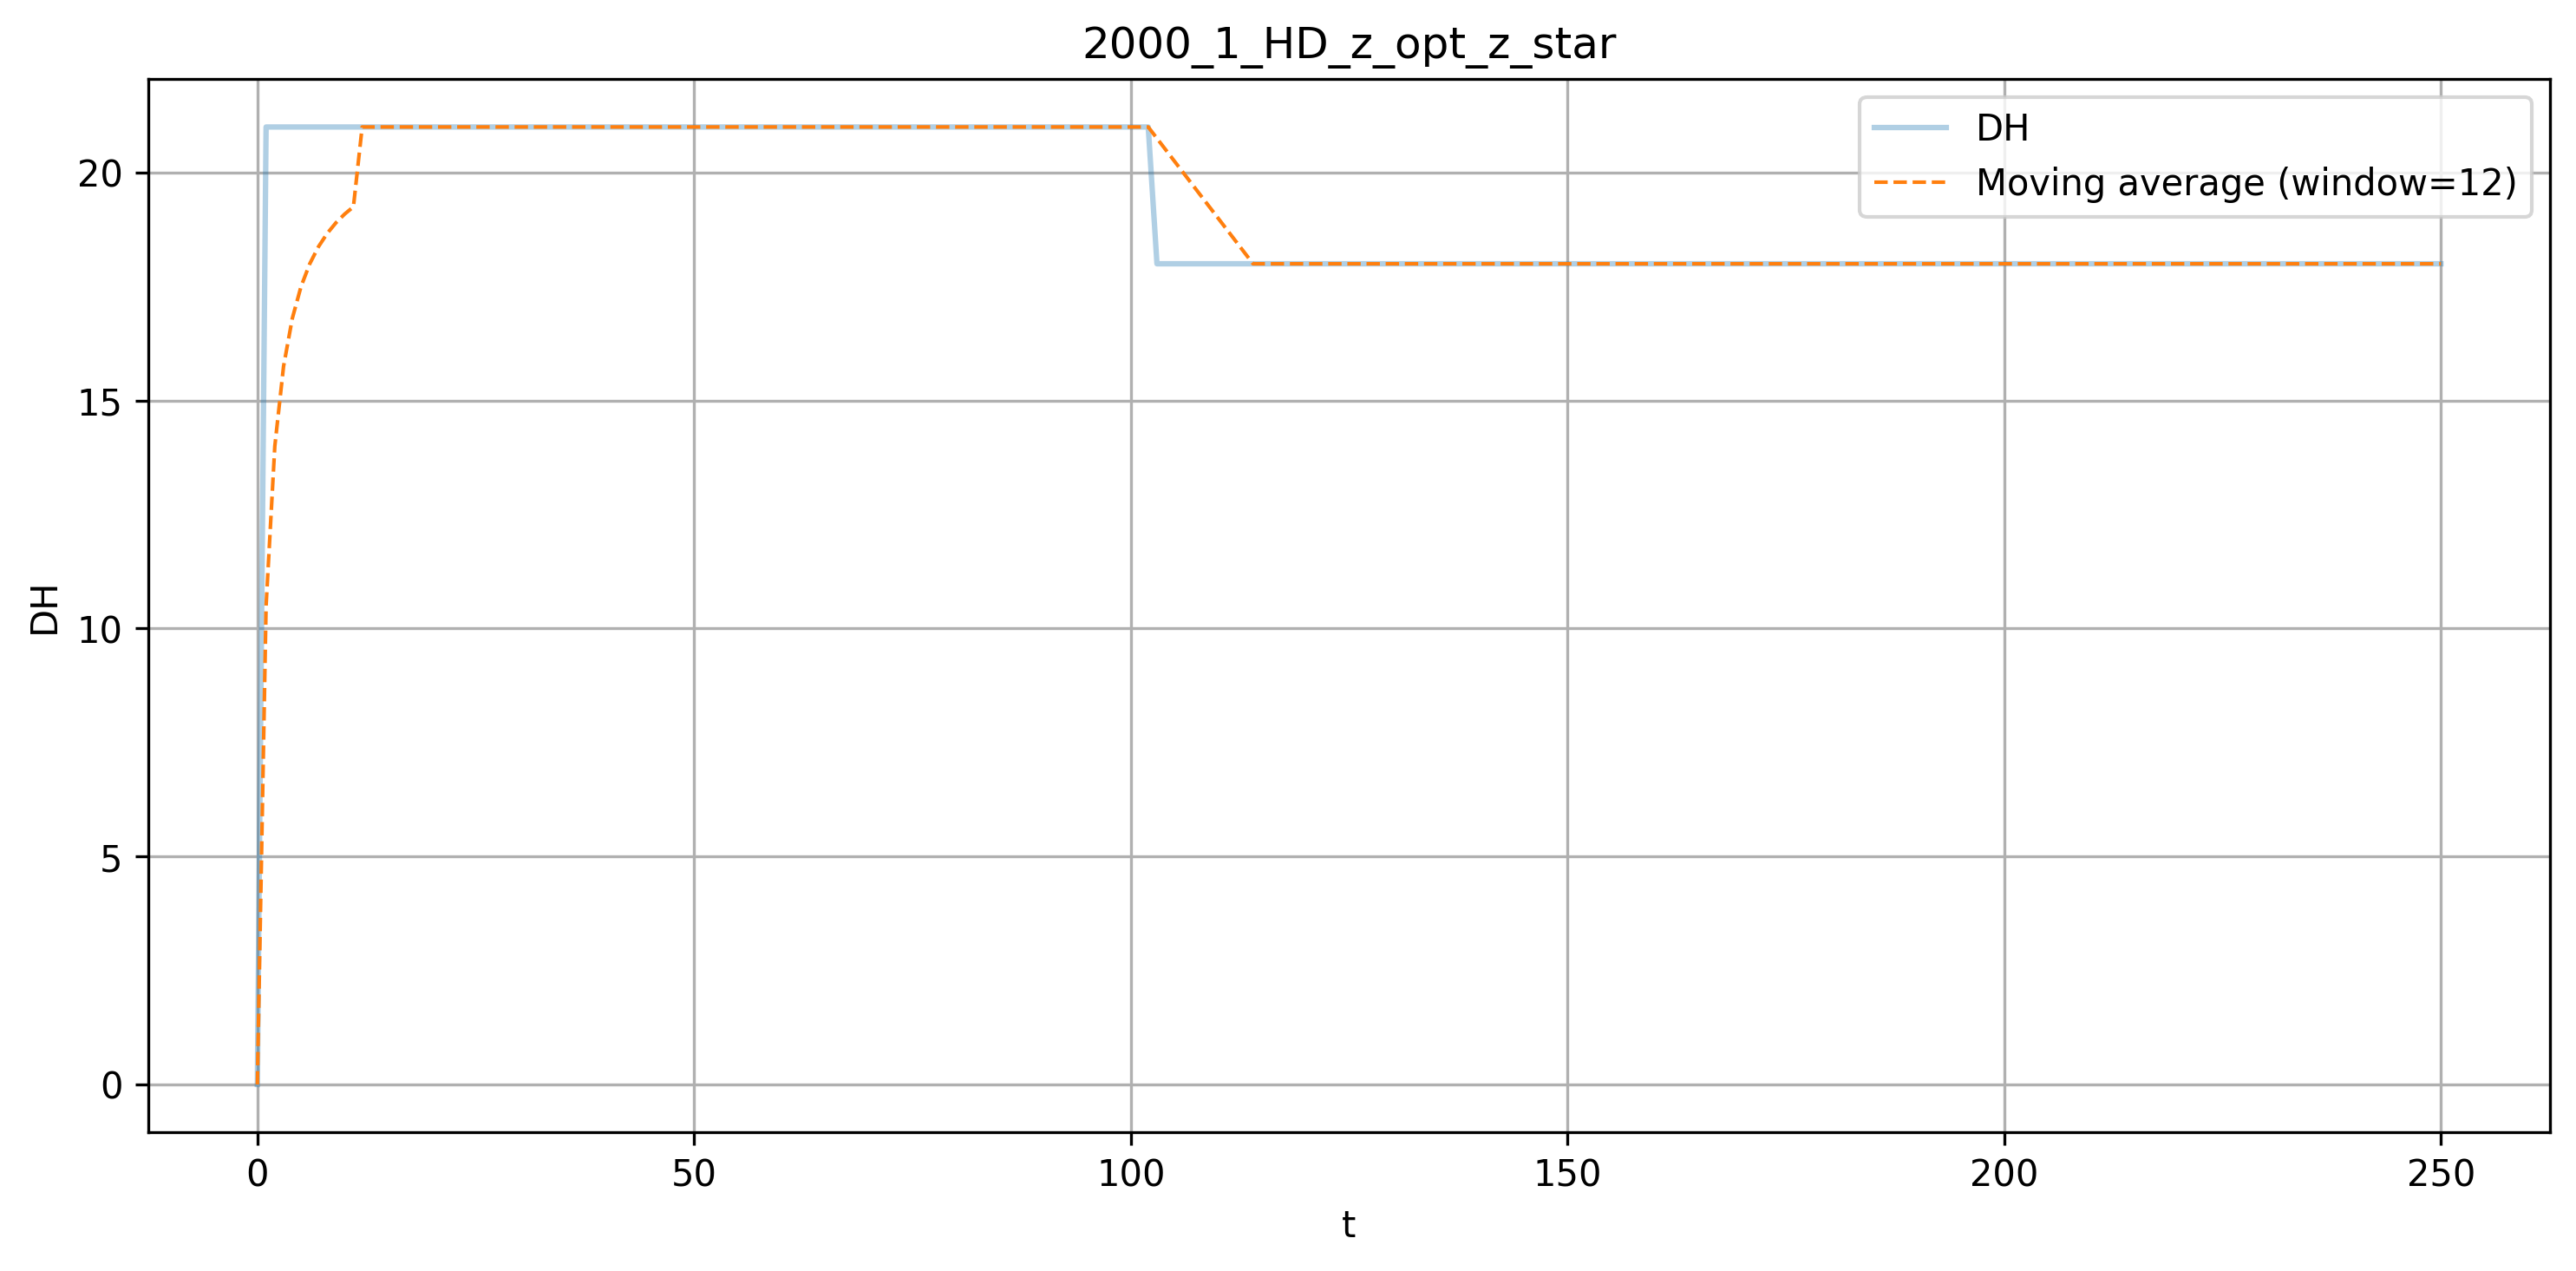
\includegraphics[width=\linewidth]{../Quantum-Annealing-for-solving-QUBO-Problems/test/Diagnostica_QALS/2/Decay_factor/ksp_2/lambda_650_dot_C/2000_1_HD_z_opt_z_star.png}
    \caption{\(d_H(z_{opt}, z_\star)\) con \(\lambda_1\)}
    \label{fig:hd-zopt-zstar-lambda1}
\end{subfigure}
\hfill
\begin{subfigure}{0.495\textwidth}
    \centering
    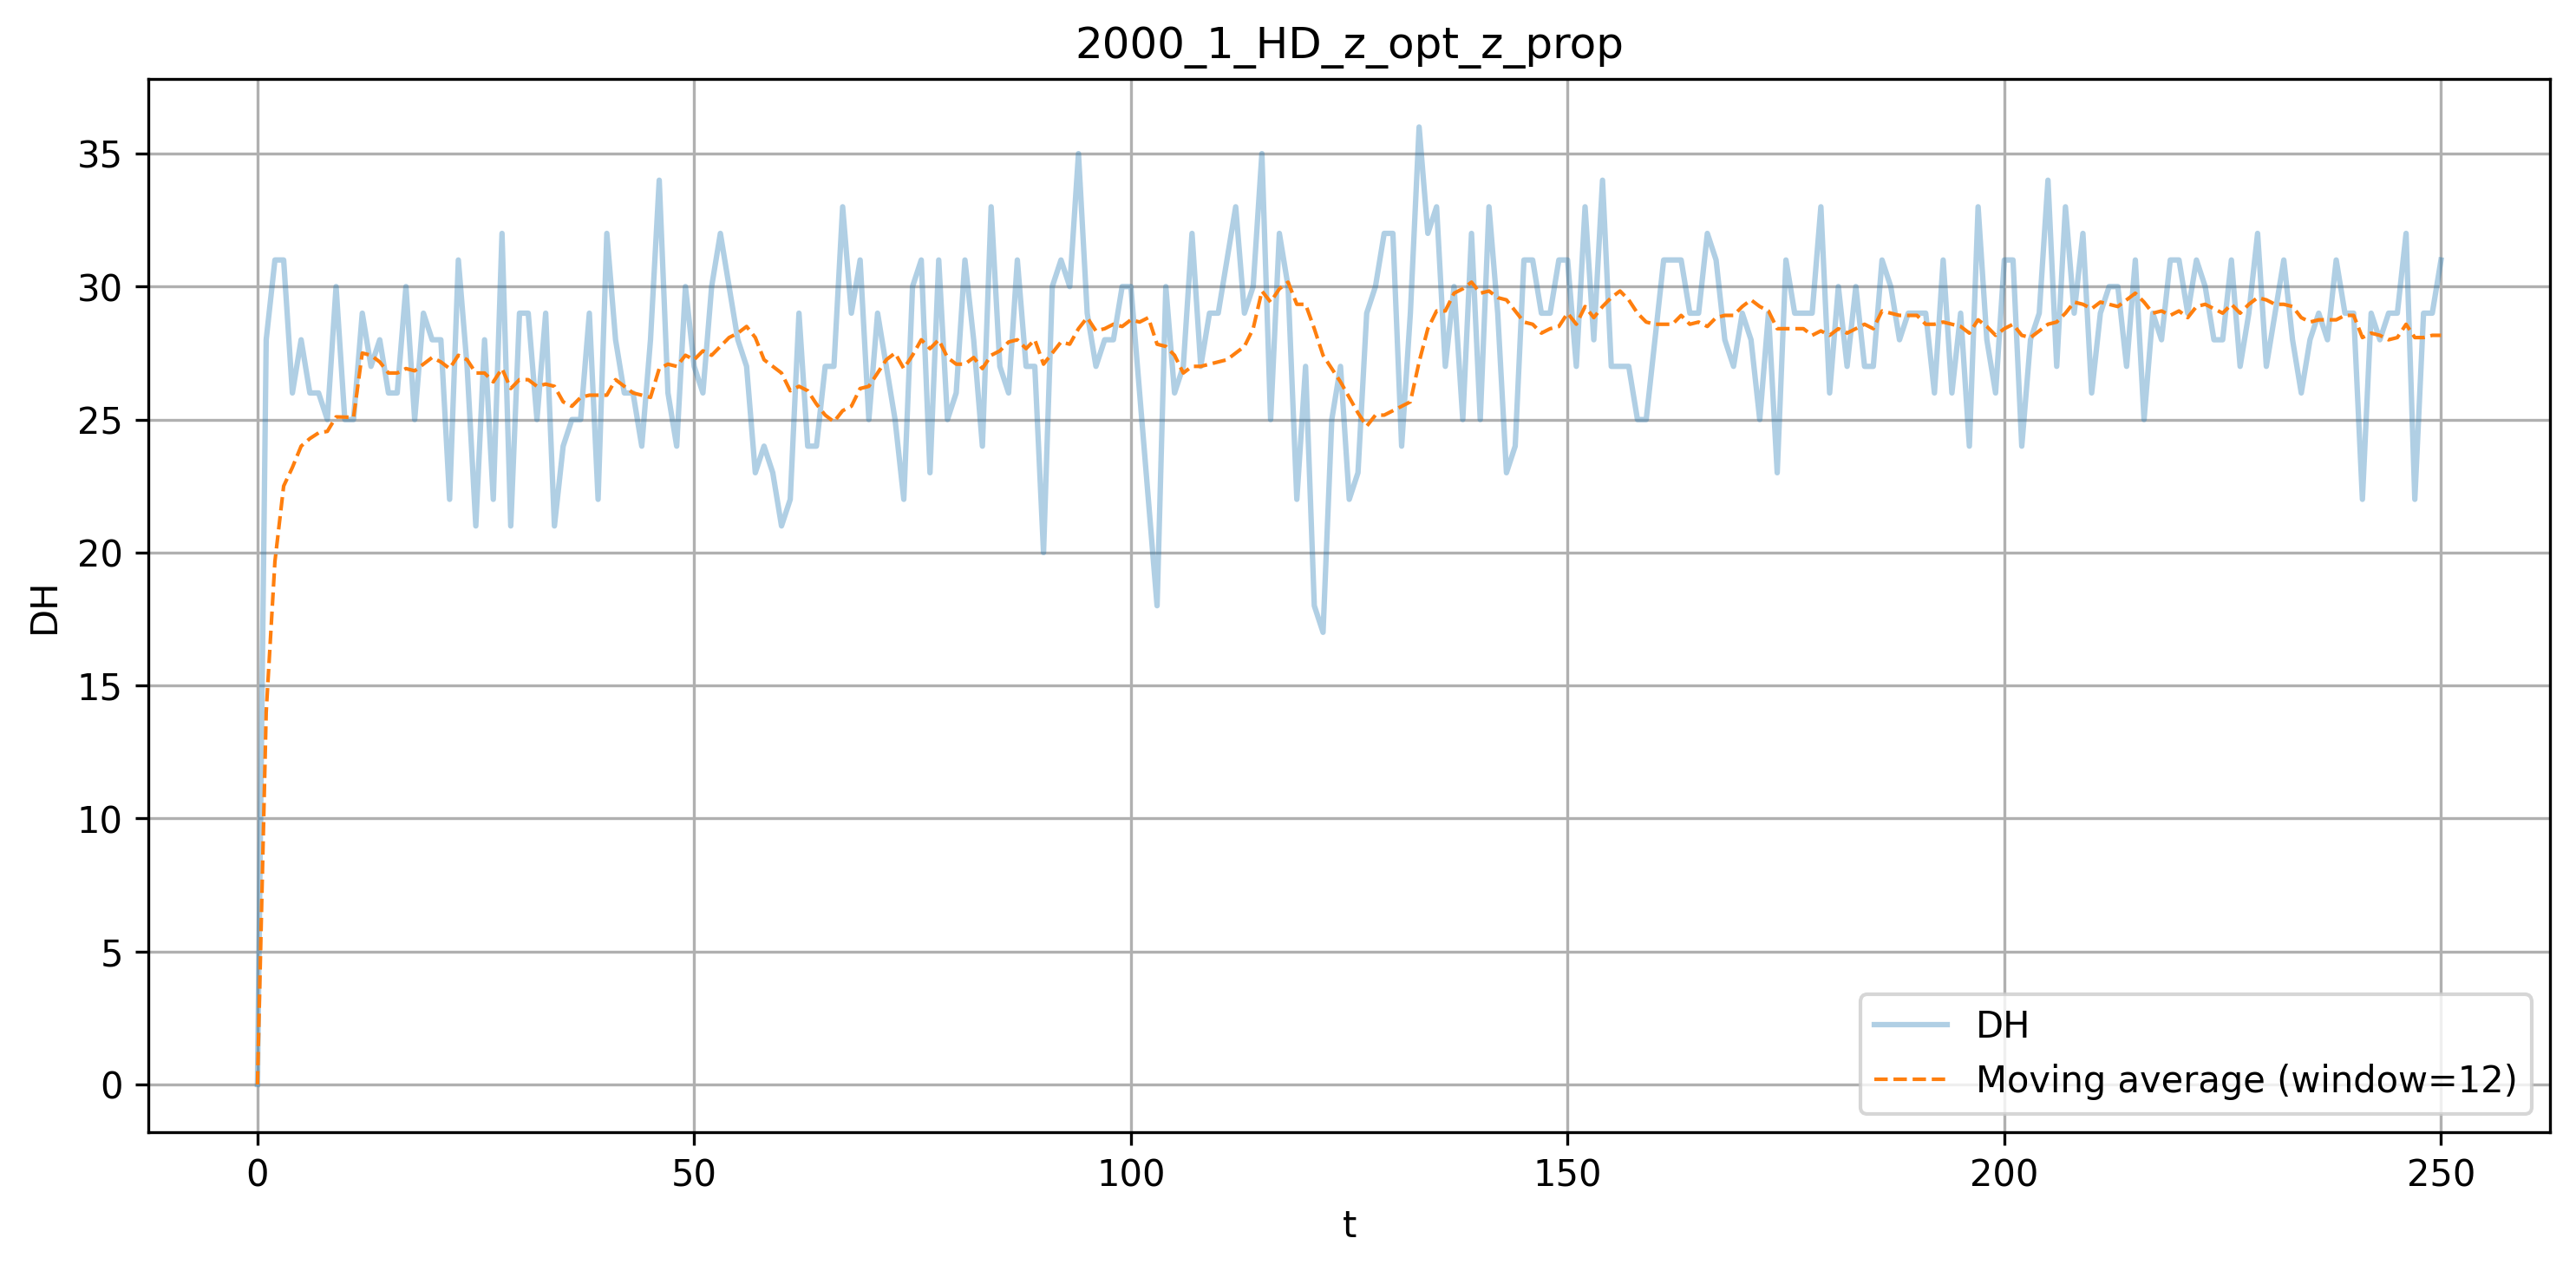
\includegraphics[width=\linewidth]{../Quantum-Annealing-for-solving-QUBO-Problems/test/Diagnostica_QALS/2/Decay_factor/ksp_2/lambda_650_dot_C/2000_1_HD_z_opt_z_prop.png}
    \caption{\(d_H(z_{opt}, z_t)\) con \(\lambda_1\)}
    \label{fig:hd-zopt-zt-lambda1}
\end{subfigure}

\vspace{0.35cm}

\begin{subfigure}{0.495\textwidth}
    \centering
    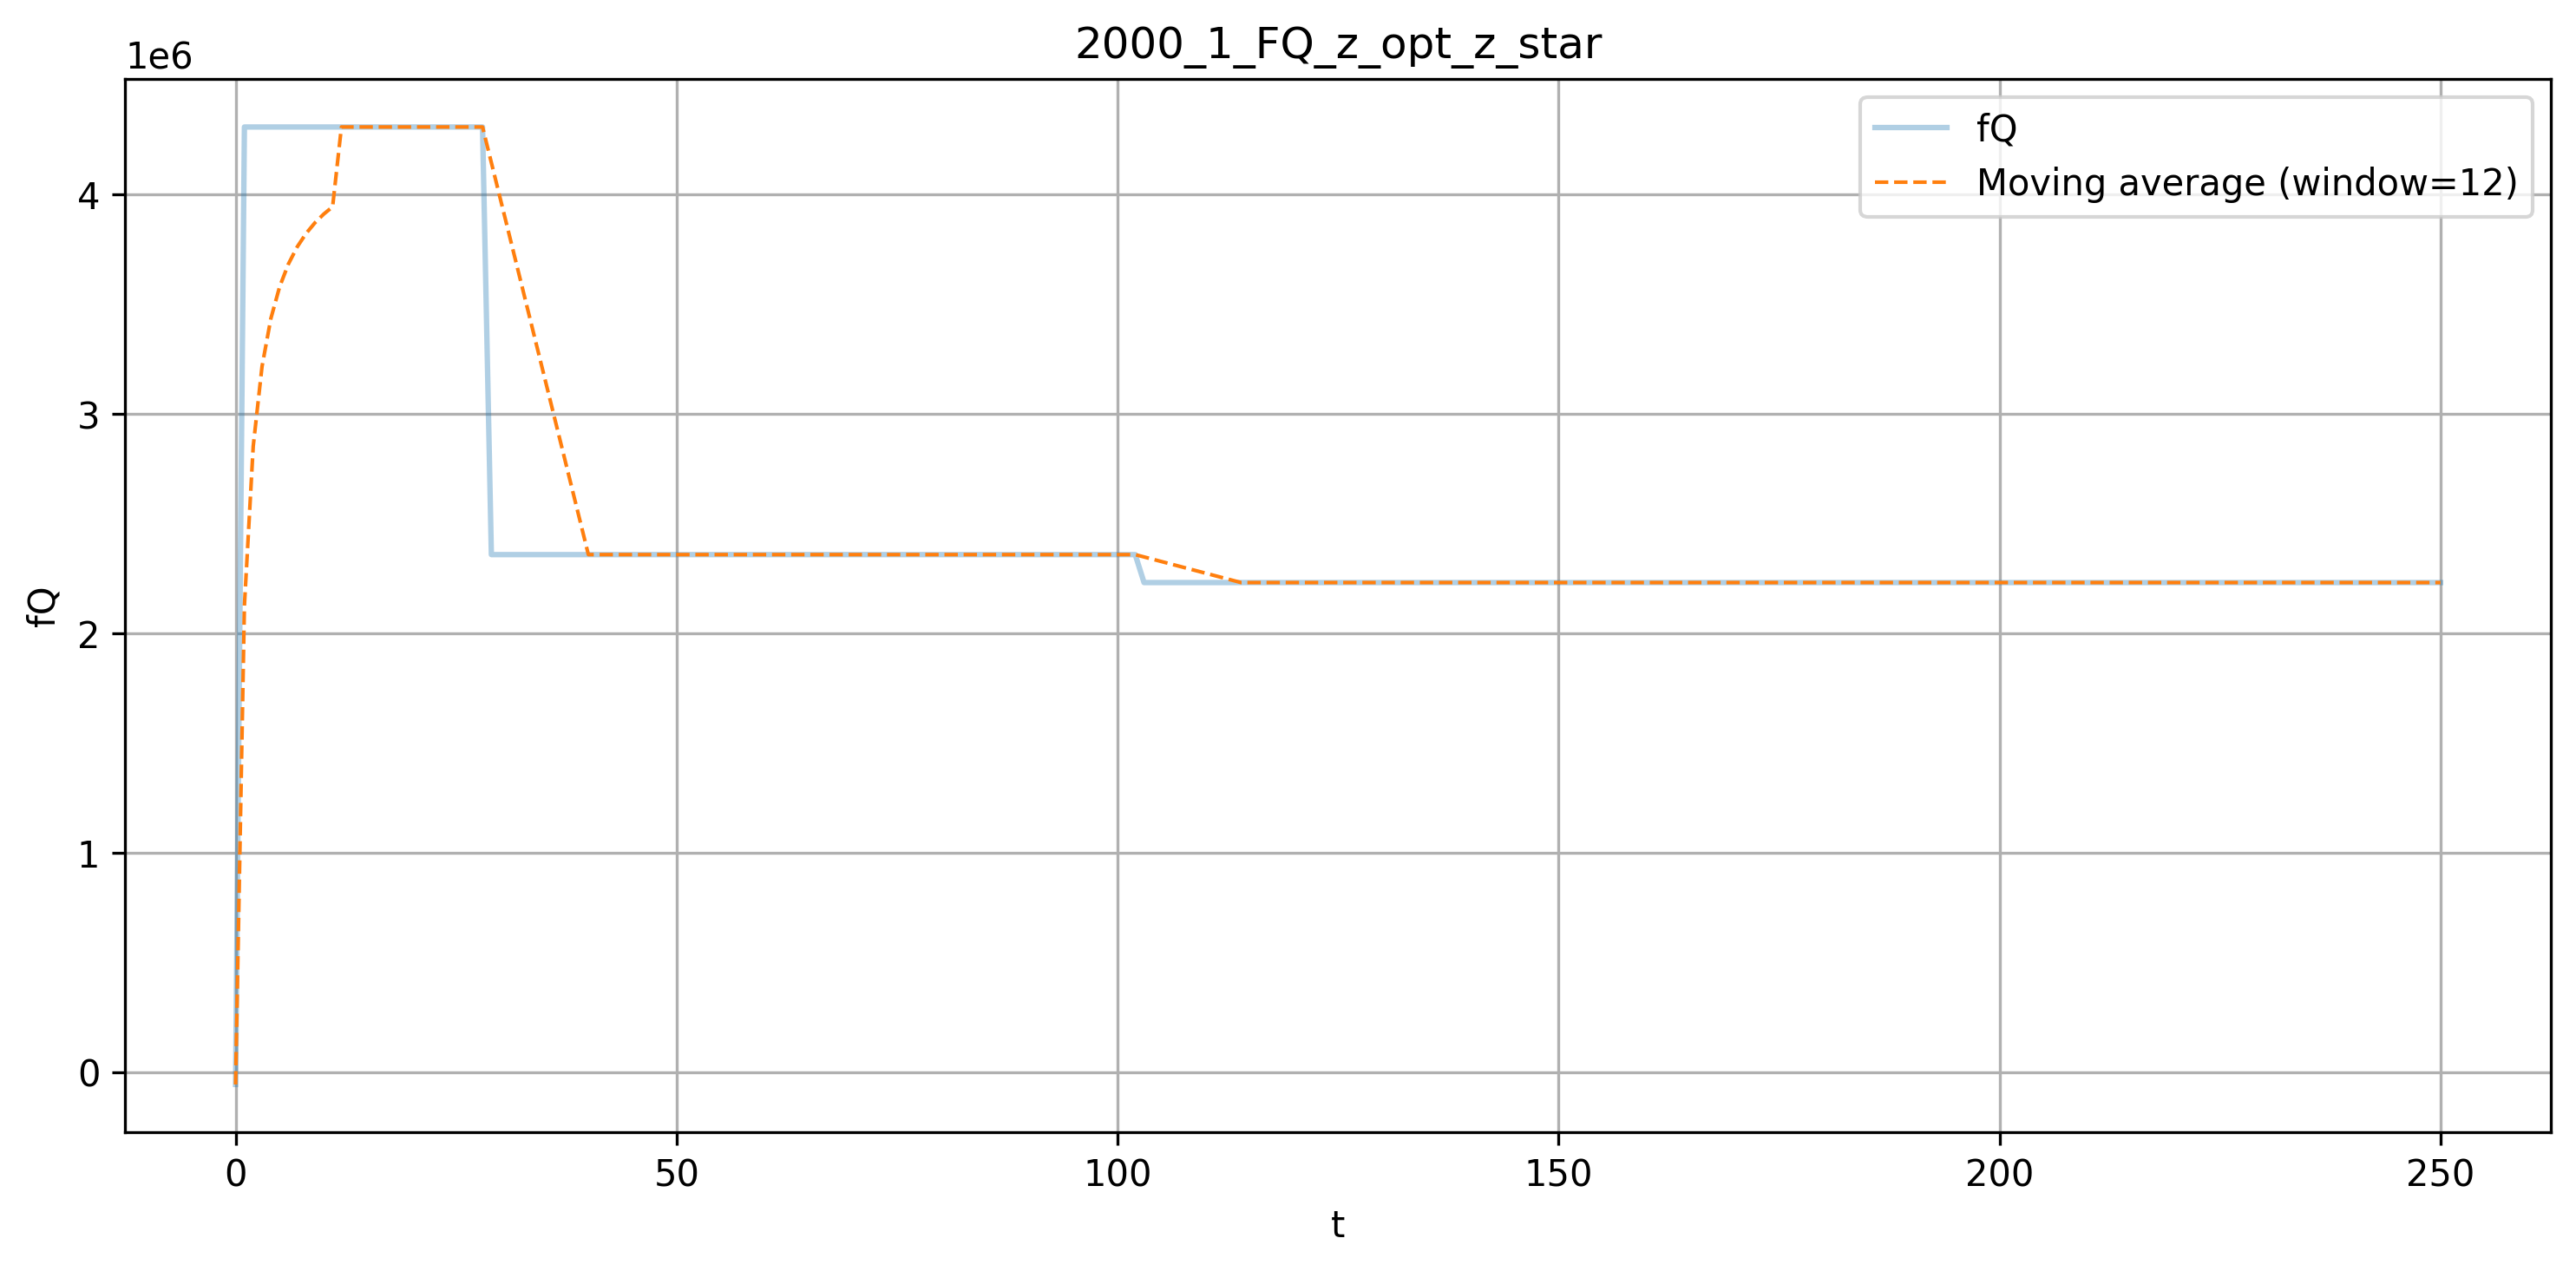
\includegraphics[width=\linewidth]{../Quantum-Annealing-for-solving-QUBO-Problems/test/Diagnostica_QALS/2/Decay_factor/ksp_2/lambda_650_dot_C/2000_1_FQ_z_opt_z_star.png}
    \caption{\(f_Q(z_\star)\) con \(\lambda_1\)}
    \label{fig:fQ-zstar-lambda1}
\end{subfigure}
\hfill
\begin{subfigure}{0.495\textwidth}
    \centering
    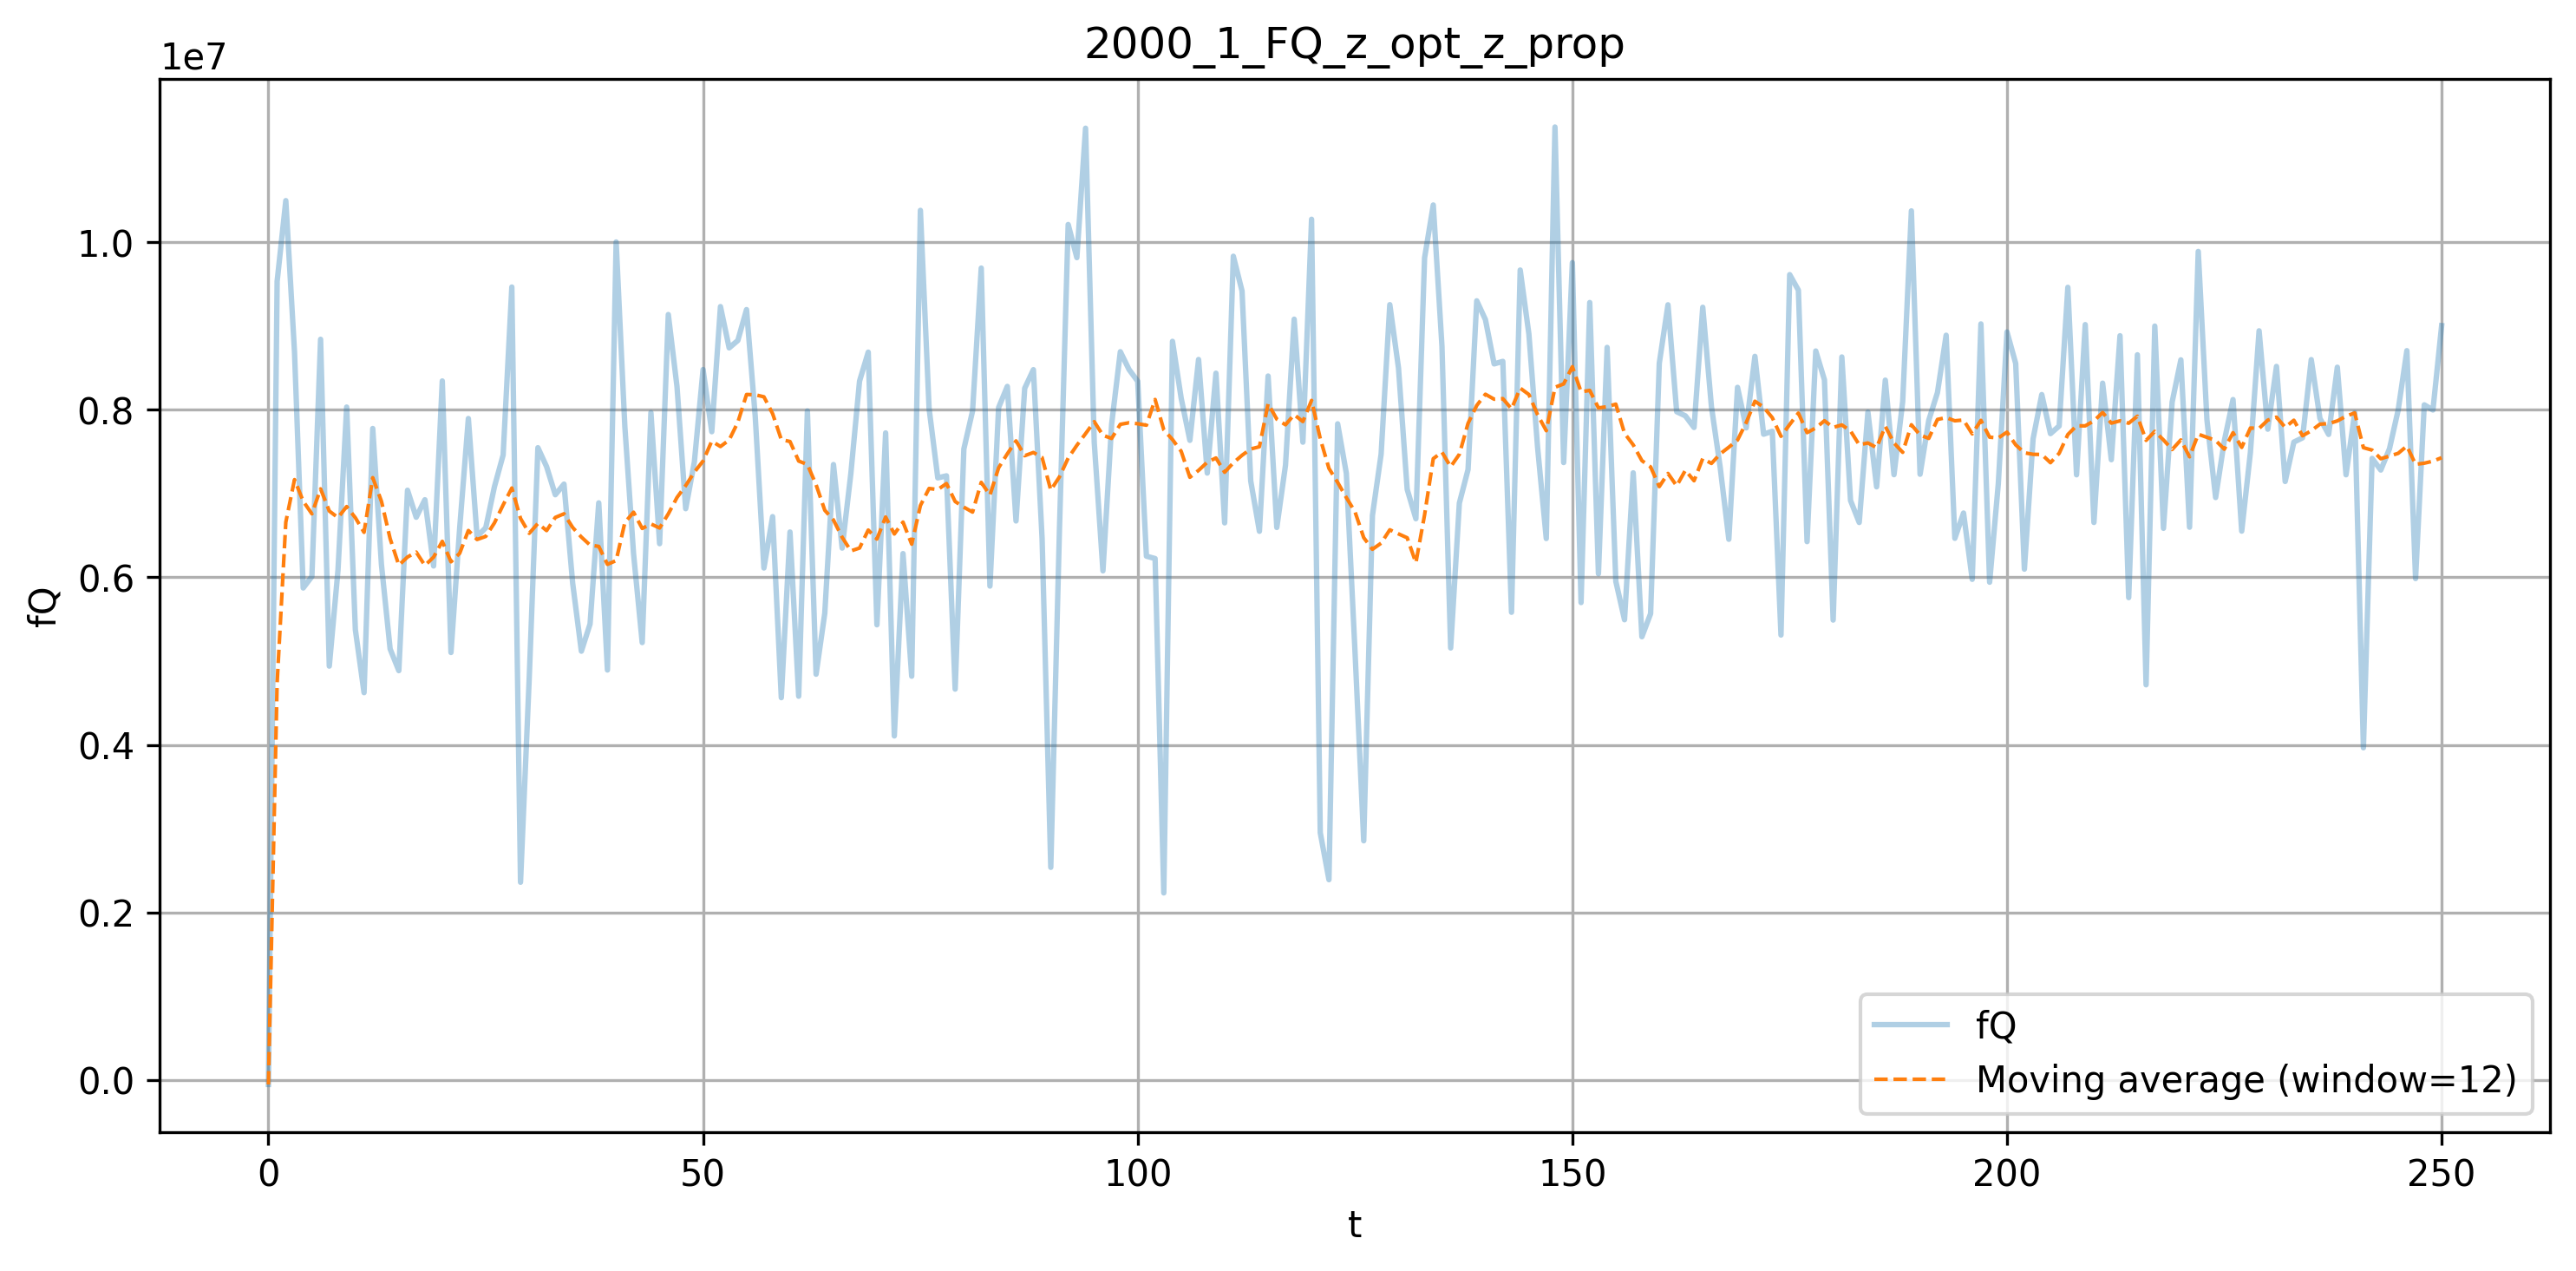
\includegraphics[width=\linewidth]{../Quantum-Annealing-for-solving-QUBO-Problems/test/Diagnostica_QALS/2/Decay_factor/ksp_2/lambda_650_dot_C/2000_1_FQ_z_opt_z_prop.png}
    \caption{\(f_Q(z_t)\) con \(\lambda_1\)}
    \label{fig:fQ-zt-lambda1}
\end{subfigure}
\label{fig:confronto-hamming-ksp21}
\end{figure}

\begin{figure}[H]
\centering
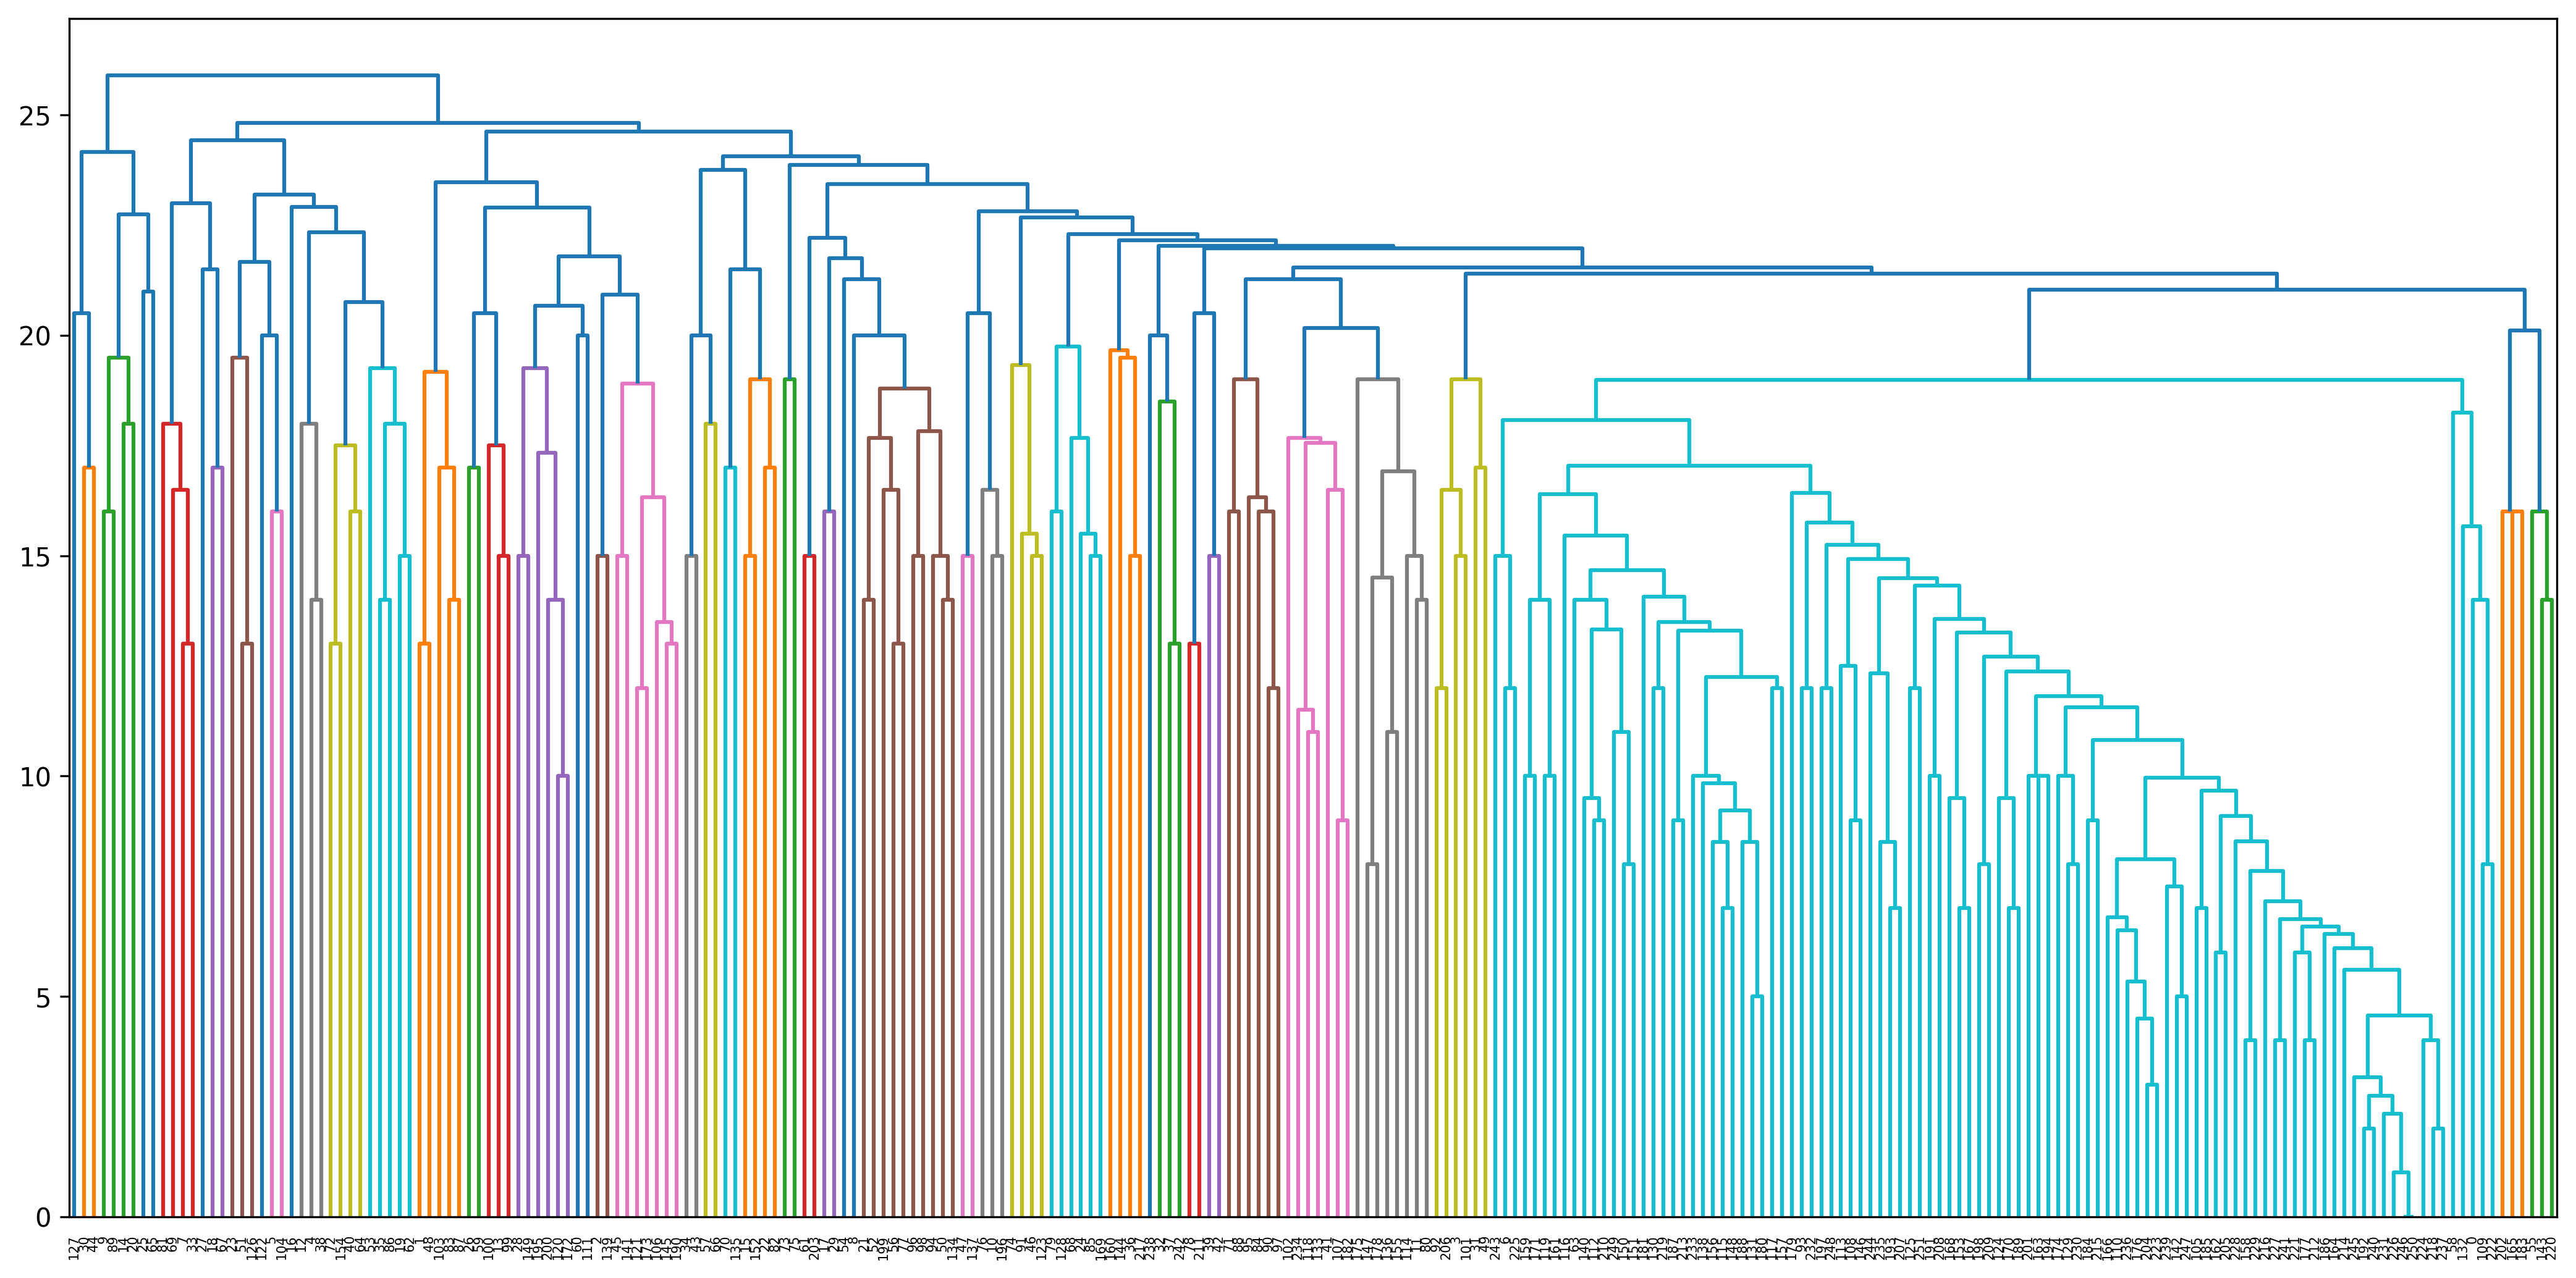
\includegraphics[width=\linewidth]{../Quantum-Annealing-for-solving-QUBO-Problems/test/Diagnostica_QALS/2/Decay_factor/ksp_2/lambda_650_dot_C/dendrogram_2000_1.png}
\caption{Agglomerative Clustering Dendogram}
\label{fig:AgglomerativeClustering-ksp2}
\end{figure}

\clearpage
\begin{figure}[H]
\centering
\begin{subfigure}{0.495\textwidth}
    \centering
    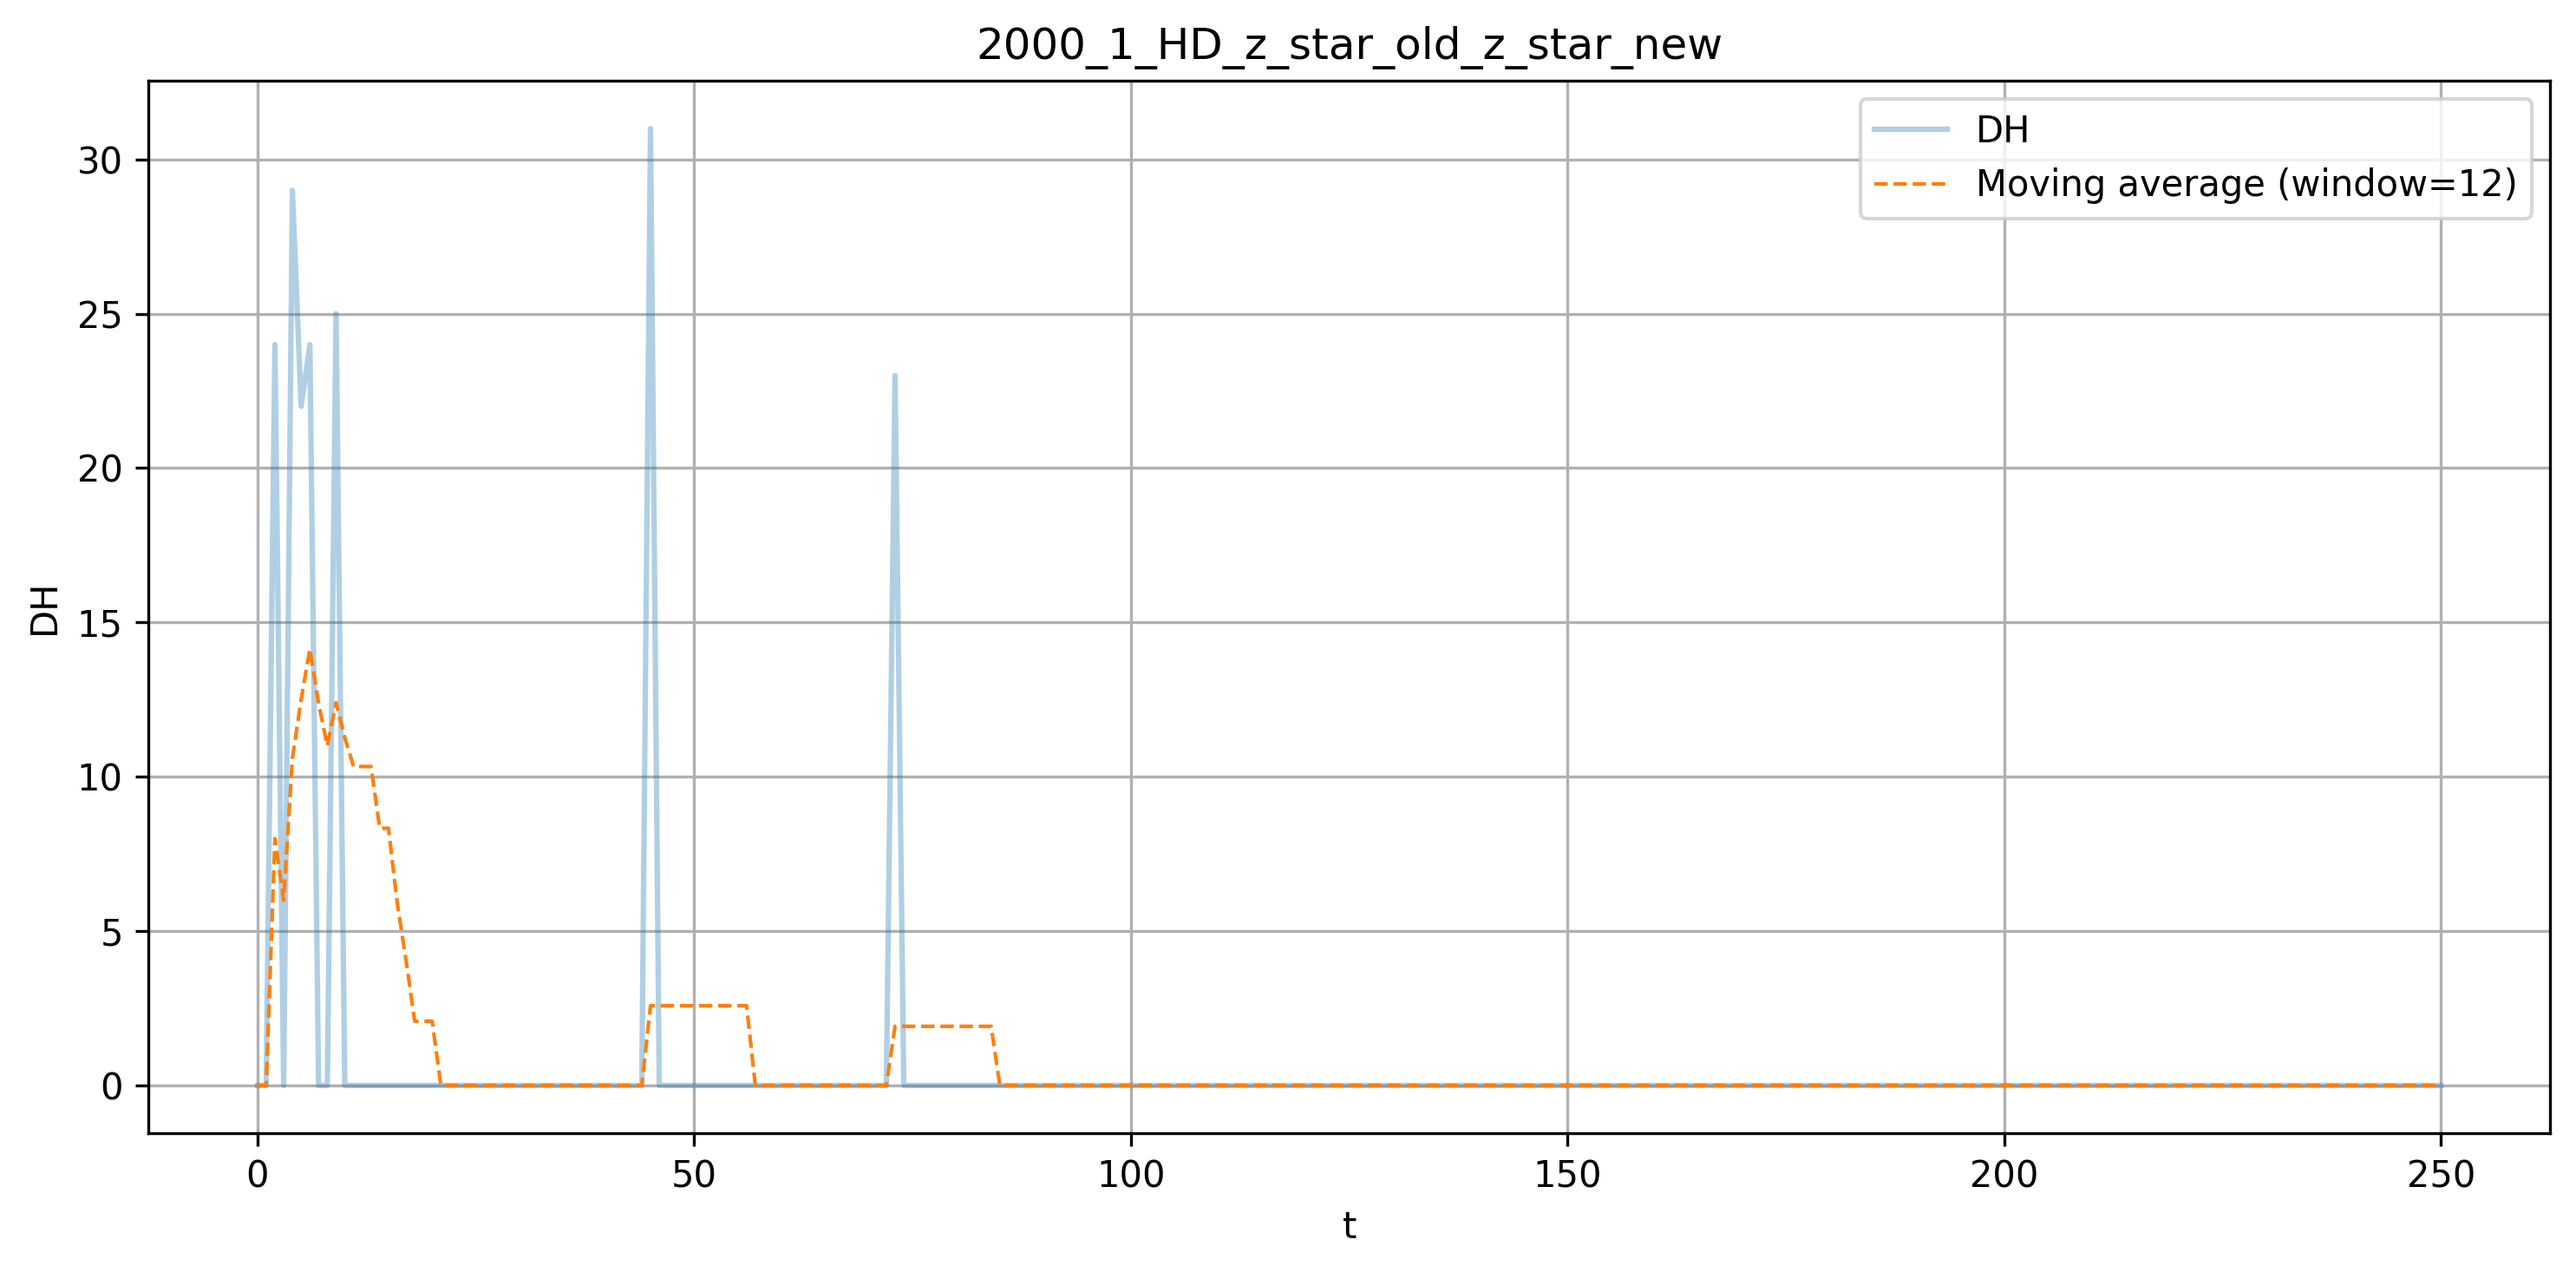
\includegraphics[width=\linewidth]{../Quantum-Annealing-for-solving-QUBO-Problems/test/Diagnostica_QALS/2/Decay_factor/ksp_2/lambda_div_3/2000_1_HD_z_star_old_z_star_new.png}
    \caption{\(d_H(z_\star^{old}, z_\star^{new})\) con \(\lambda_2\)}
    \label{fig:hd-zstarold-zstarnew-lambda2}
\end{subfigure}
\hfill
\begin{subfigure}{0.495\textwidth}
    \centering
    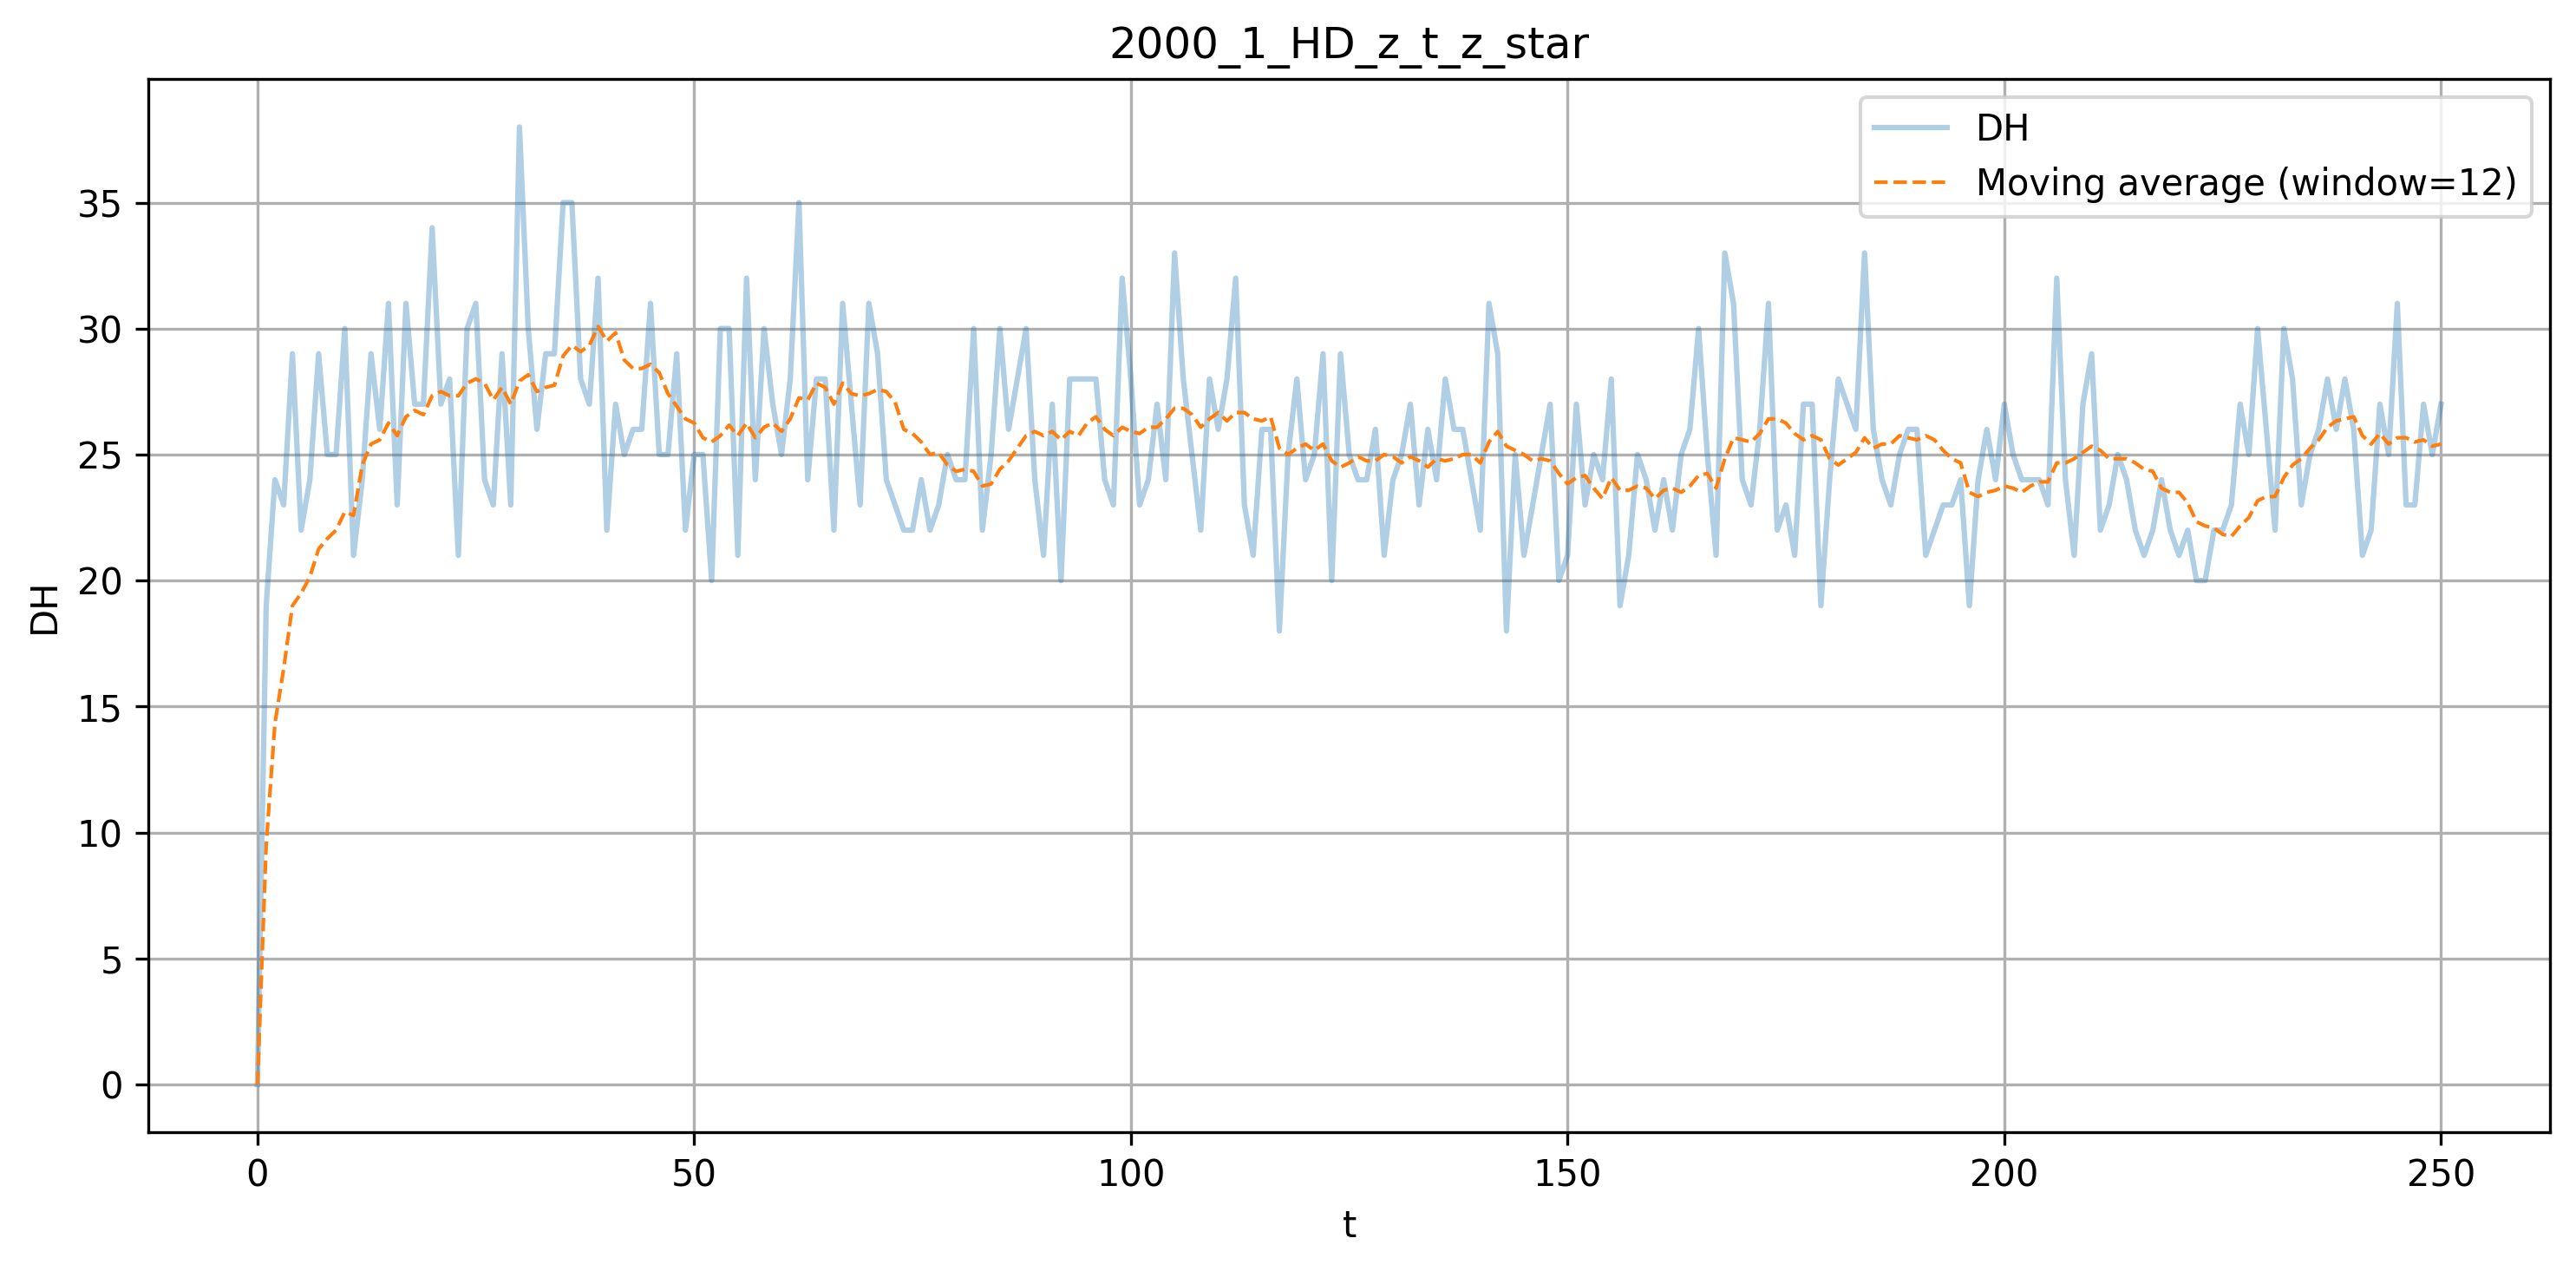
\includegraphics[width=\linewidth]{../Quantum-Annealing-for-solving-QUBO-Problems/test/Diagnostica_QALS/2/Decay_factor/ksp_2/lambda_div_3/2000_1_HD_z_t_z_star.png}
    \caption{\(d_H(z_t, z_\star)\) con \(\lambda_2\)}
    \label{fig:hd-zt-zstar-lambda2}
\end{subfigure}

\vspace{0.35cm}

\begin{subfigure}{0.495\textwidth}
    \centering
    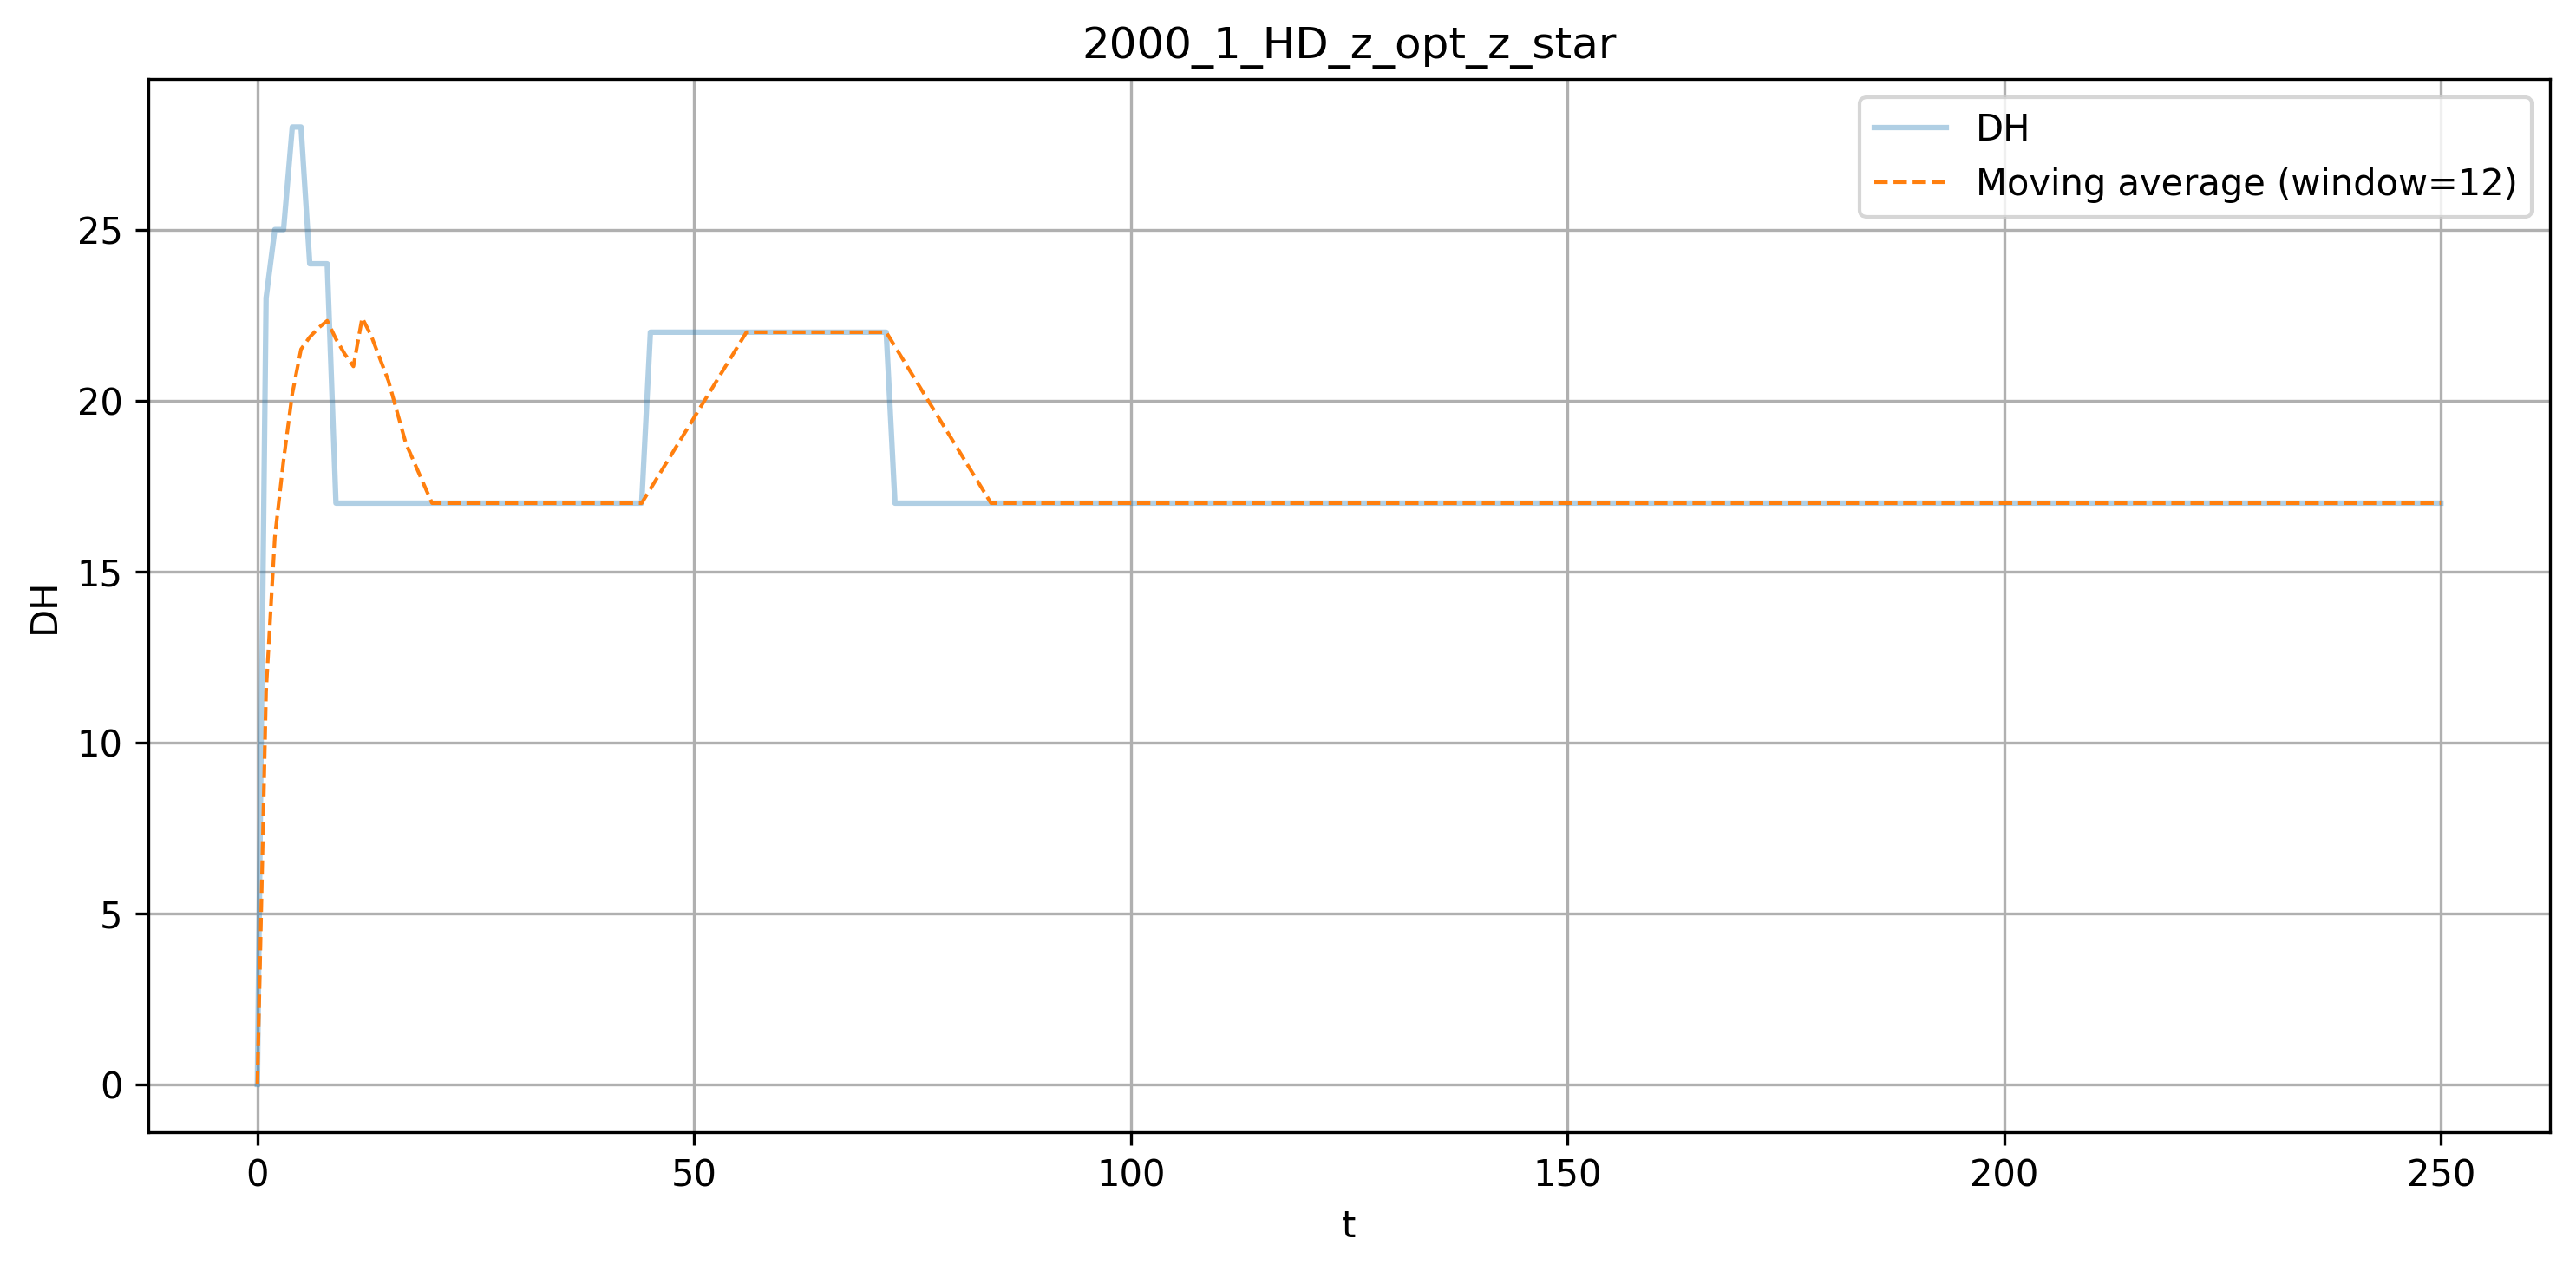
\includegraphics[width=\linewidth]{../Quantum-Annealing-for-solving-QUBO-Problems/test/Diagnostica_QALS/2/Decay_factor/ksp_2/lambda_div_3/2000_1_HD_z_opt_z_star.png}
    \caption{\(d_H(z_{opt}, z_\star)\) con \(\lambda_2\)}
    \label{fig:hd-zopt-zstar-lambda2}
\end{subfigure}
\hfill
\begin{subfigure}{0.495\textwidth}
    \centering
    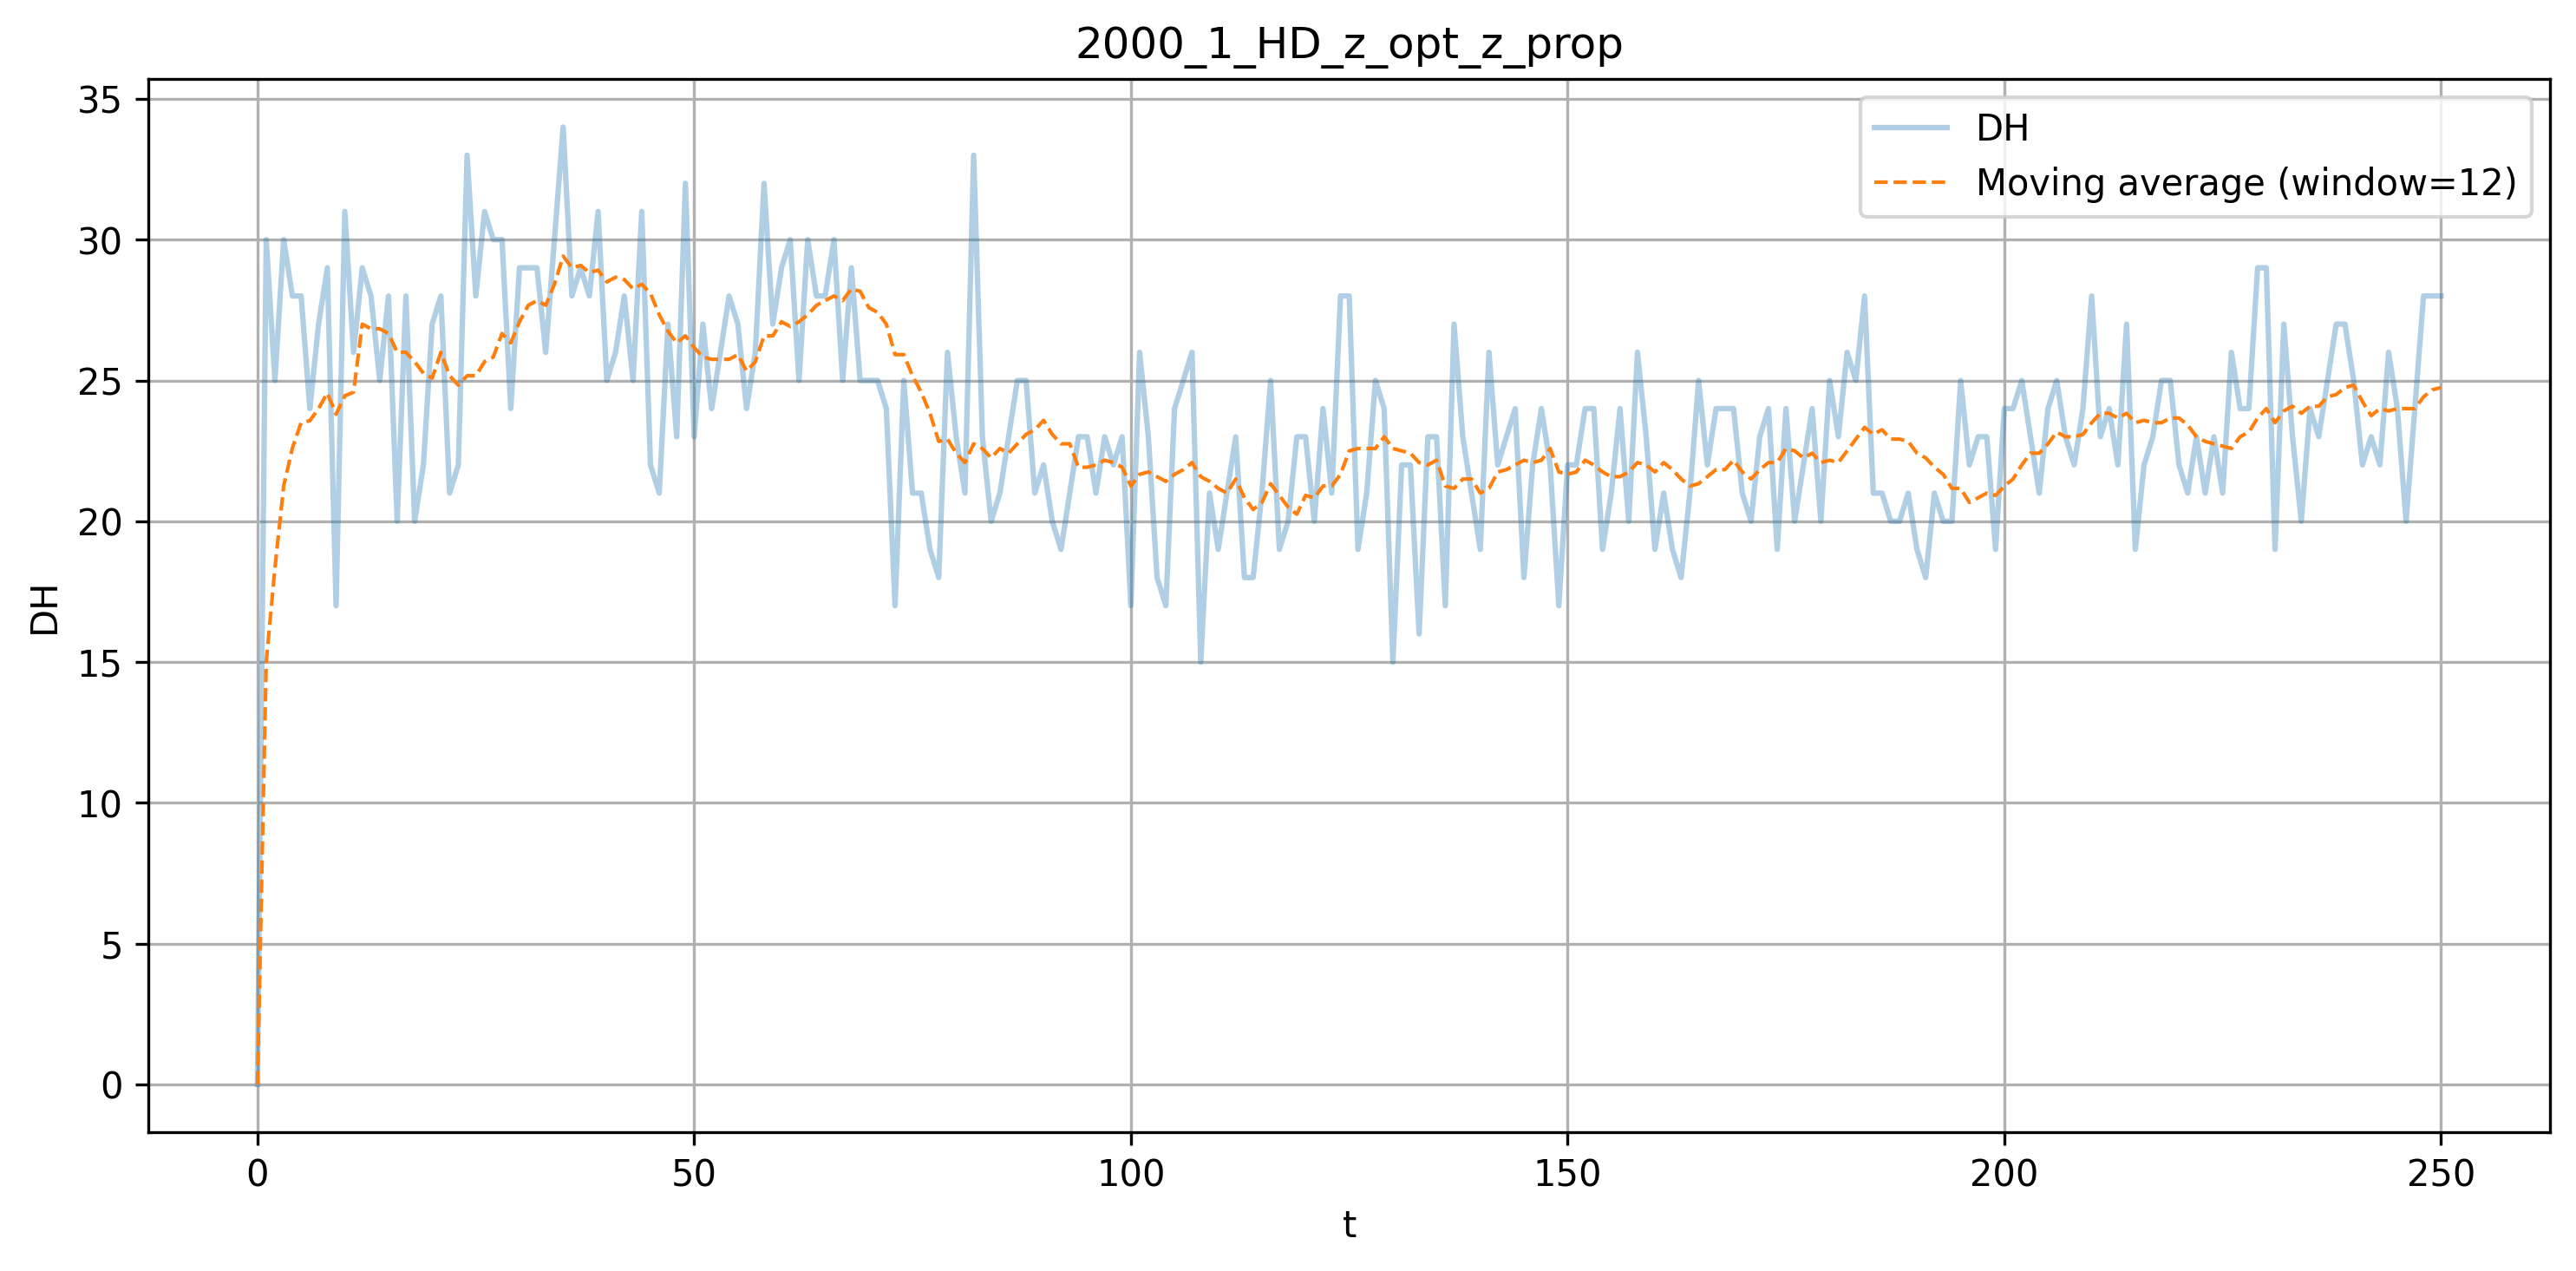
\includegraphics[width=\linewidth]{../Quantum-Annealing-for-solving-QUBO-Problems/test/Diagnostica_QALS/2/Decay_factor/ksp_2/lambda_div_3/2000_1_HD_z_opt_z_prop.png}
    \caption{\(d_H(z_{opt}, z_t)\) con \(\lambda_2\)}
    \label{fig:hd-zopt-zt-lambda2}
\end{subfigure}

\vspace{0.35cm}

\begin{subfigure}{0.495\textwidth}
    \centering
    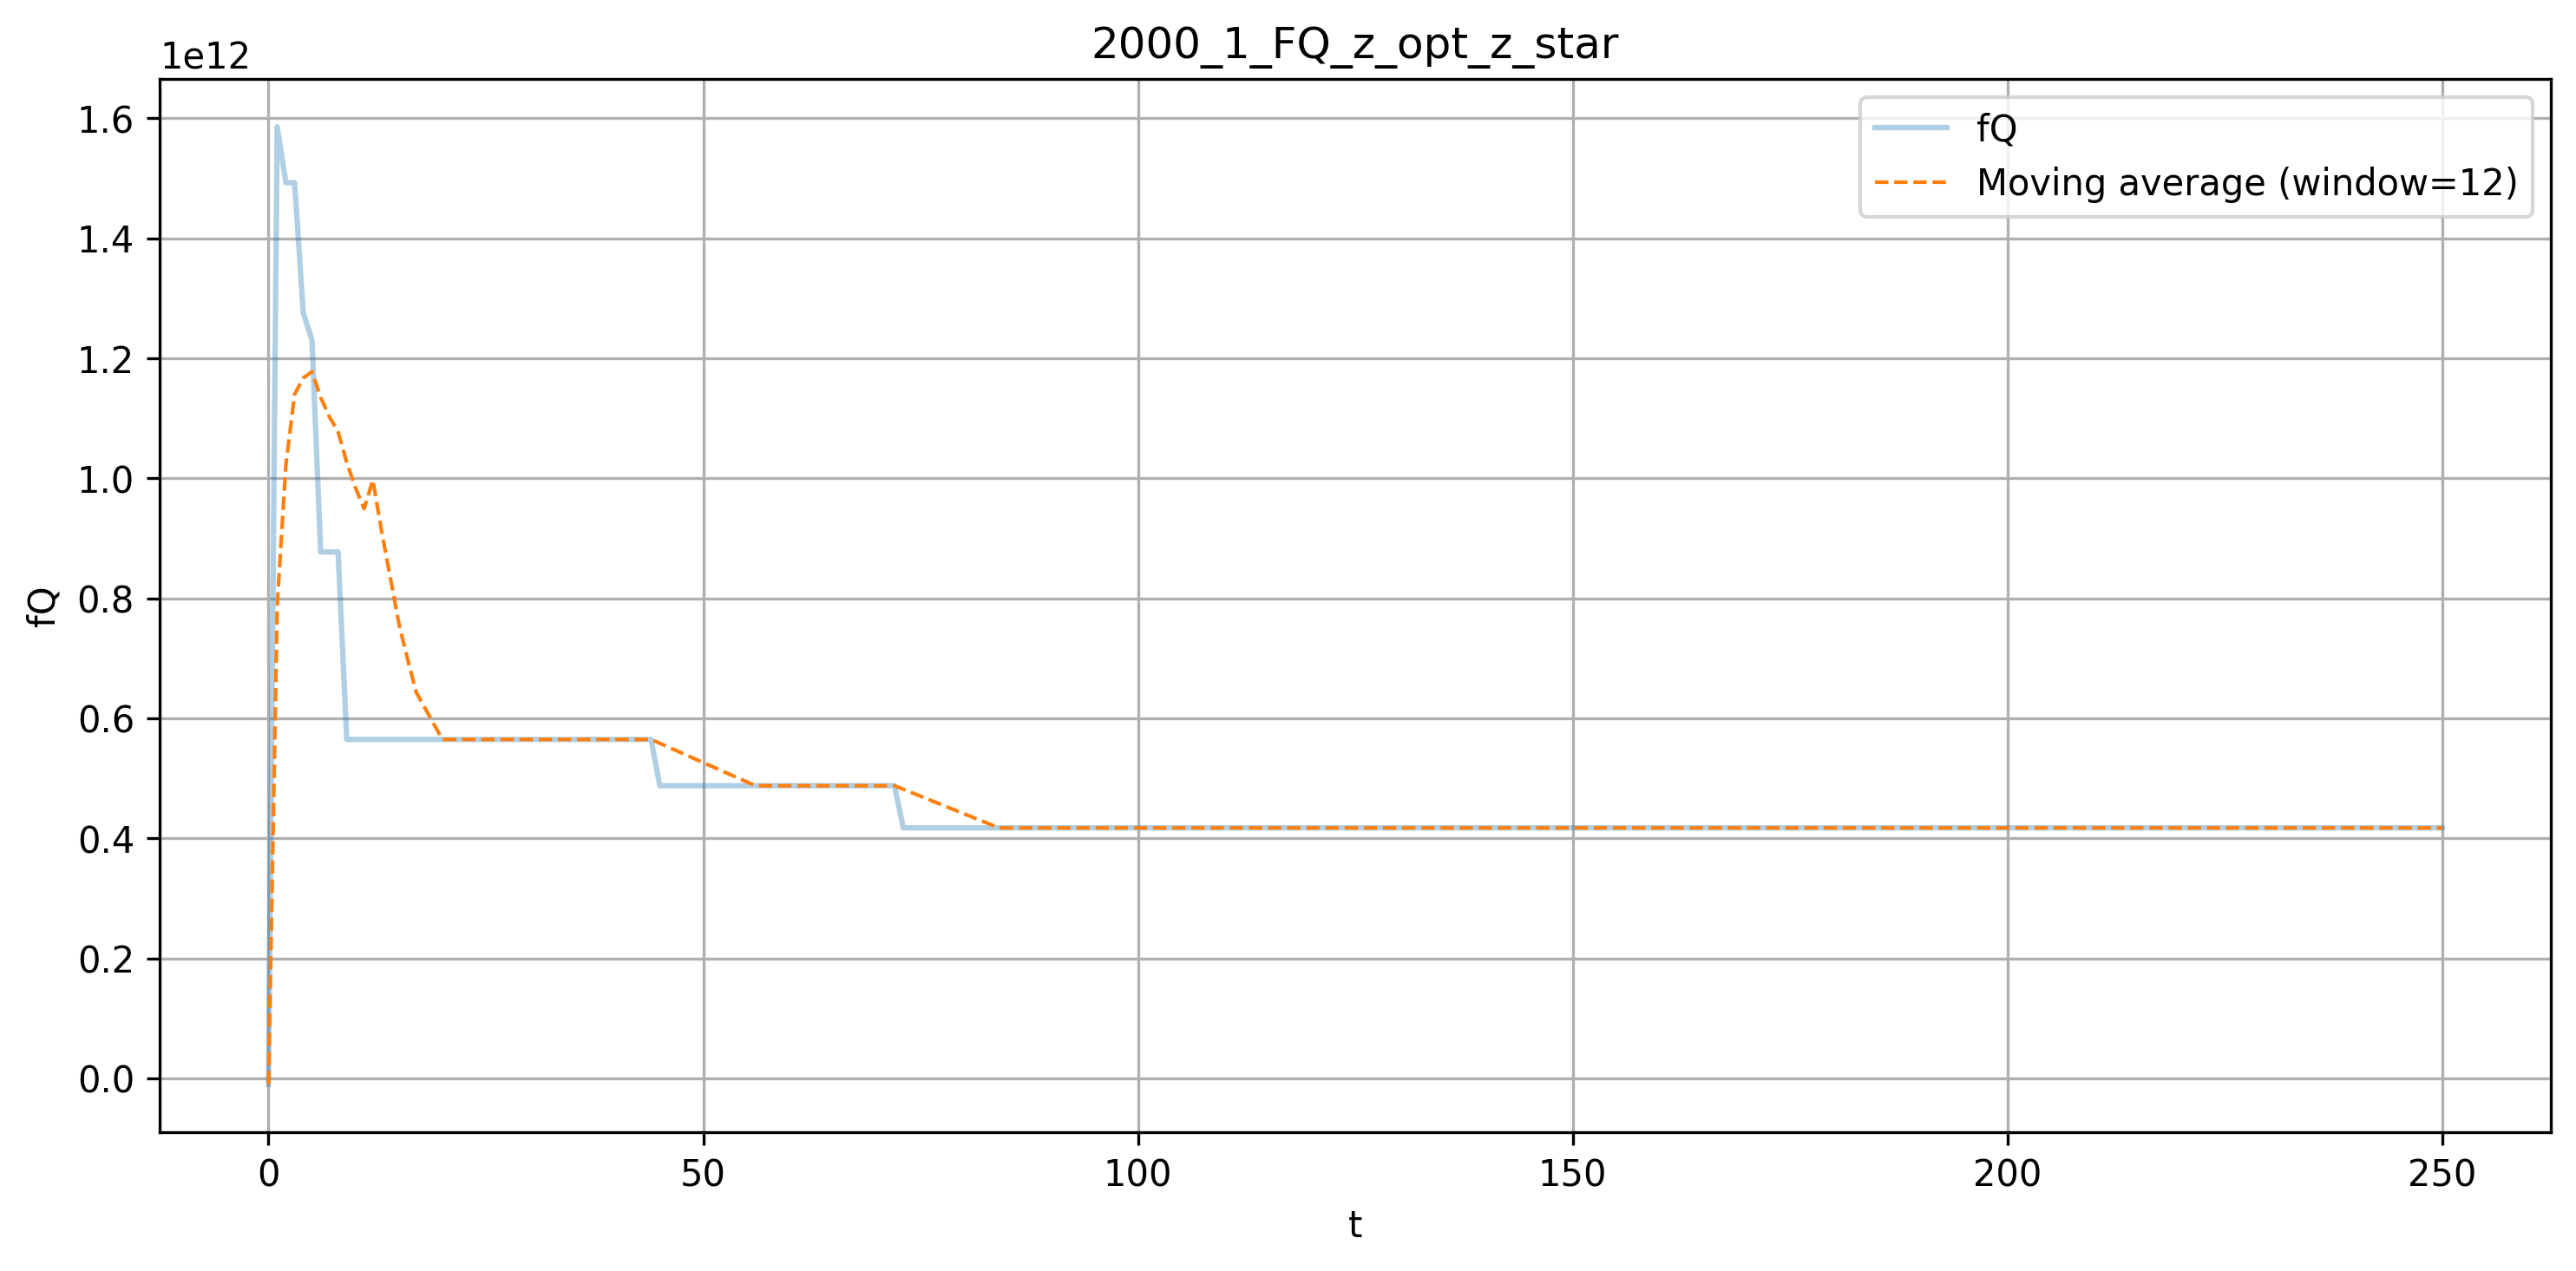
\includegraphics[width=\linewidth]{../Quantum-Annealing-for-solving-QUBO-Problems/test/Diagnostica_QALS/2/Decay_factor/ksp_2/lambda_div_3/2000_1_FQ_z_opt_z_star.png}
    \caption{\(f_Q(z_\star)\) con \(\lambda_2\)}
    \label{fig:fQ-zstar-lambda2}
\end{subfigure}
\hfill
\begin{subfigure}{0.495\textwidth}
    \centering
    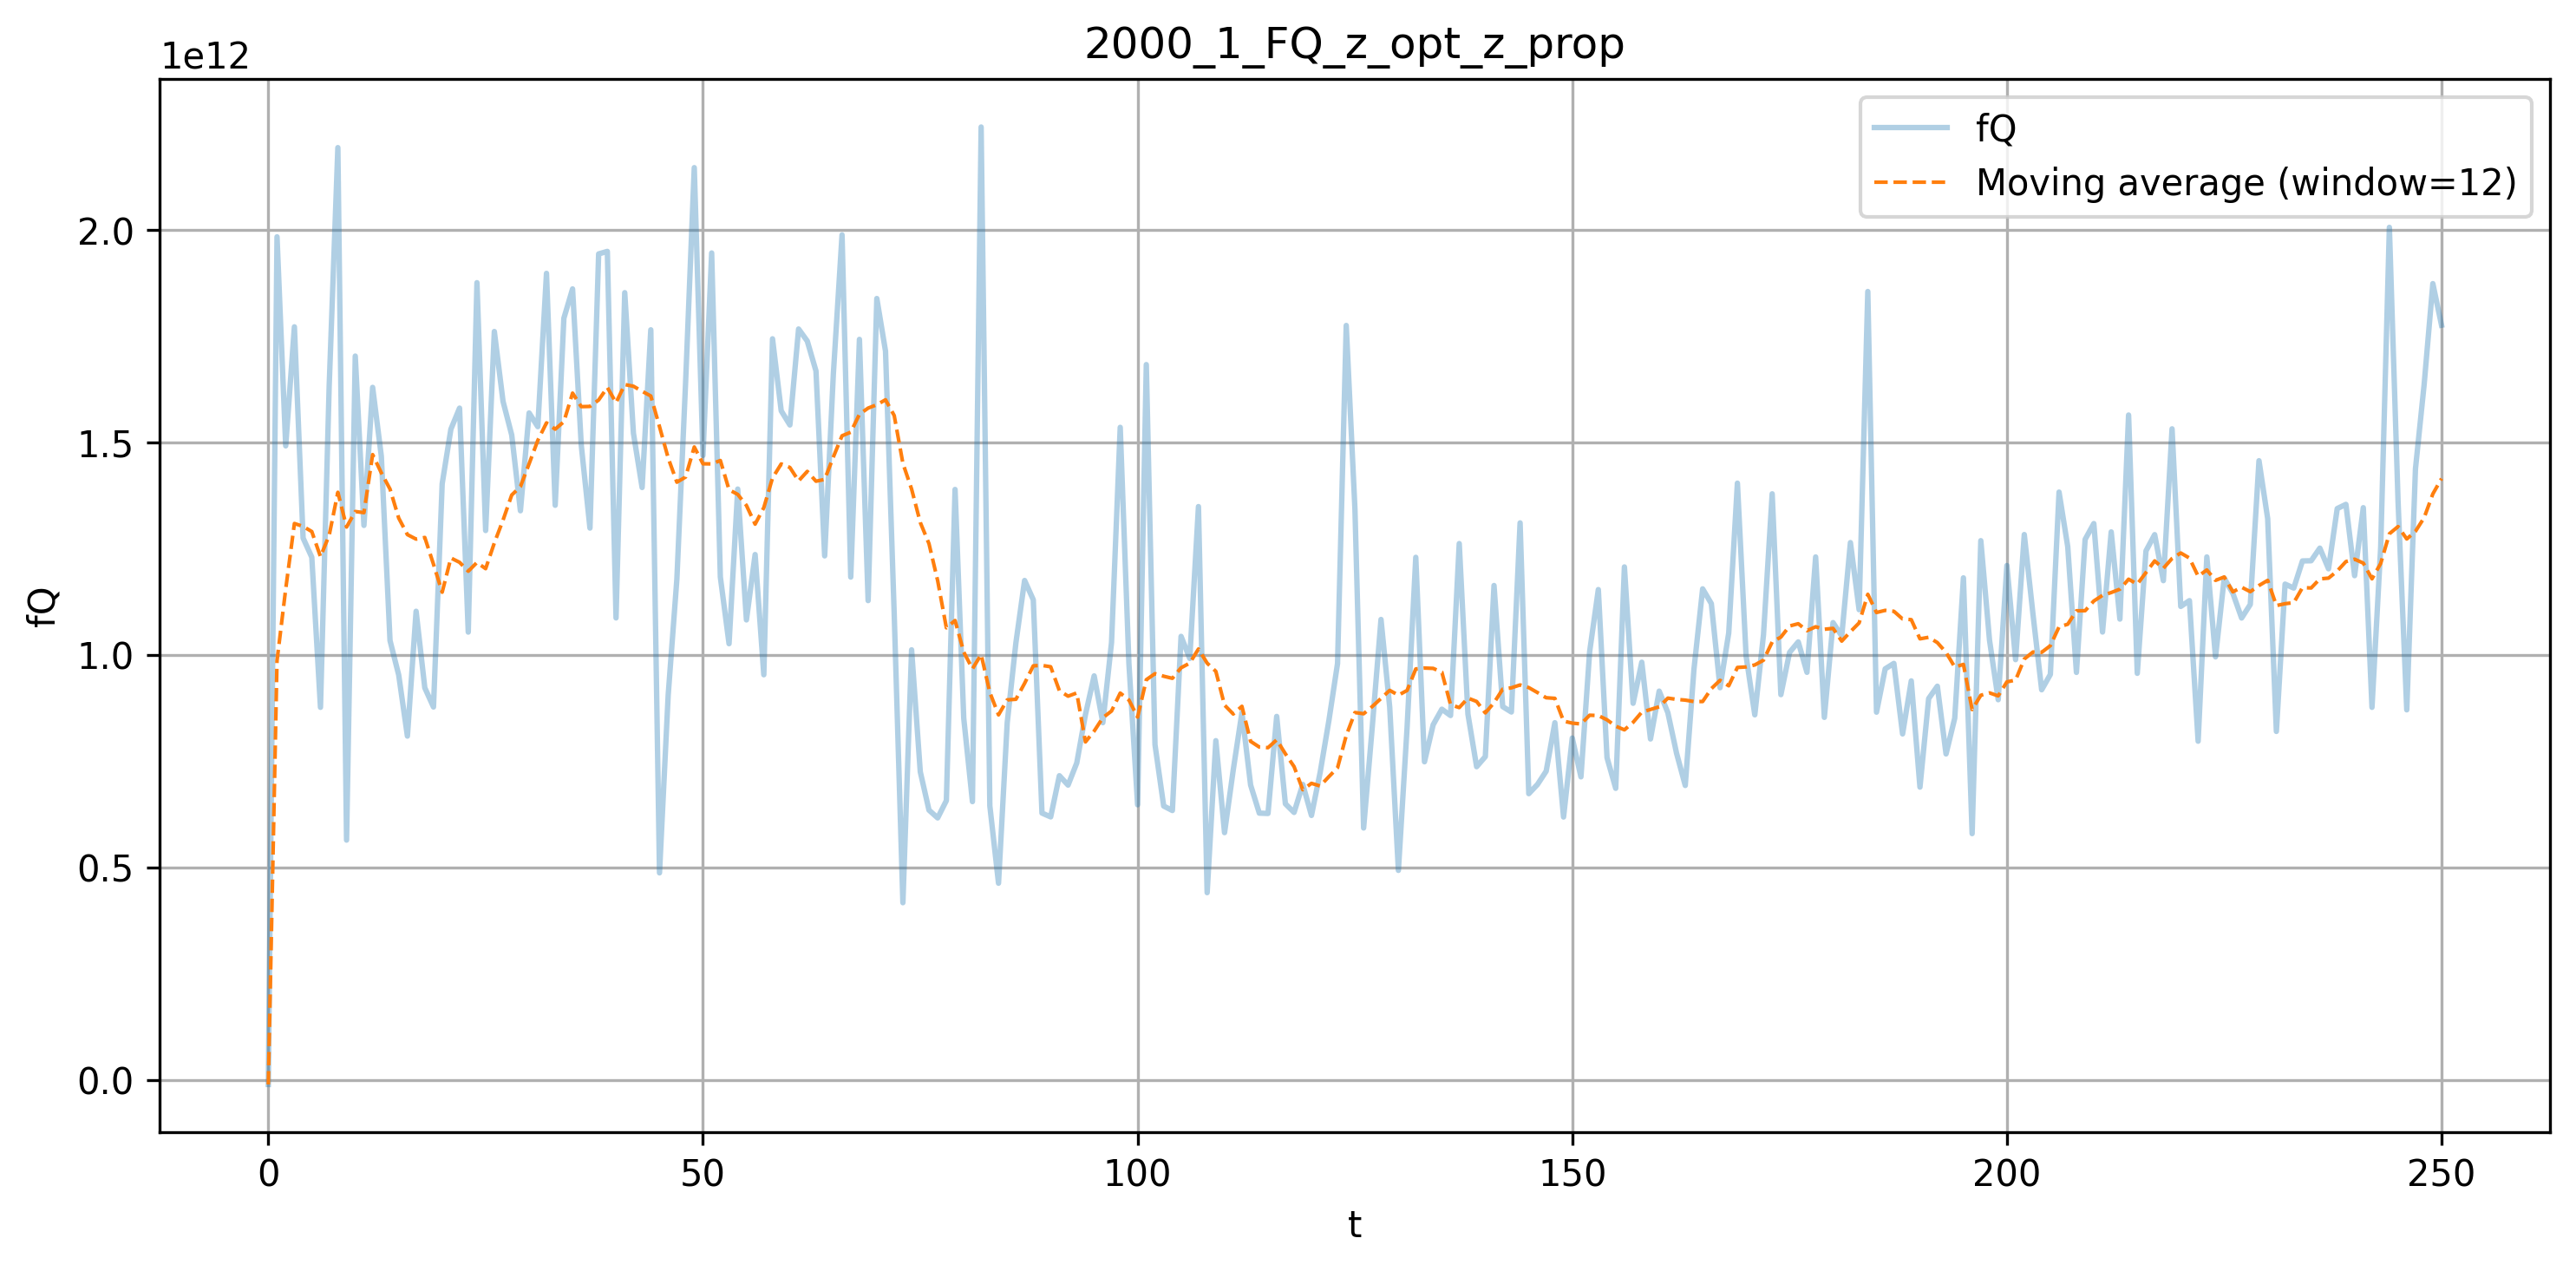
\includegraphics[width=\linewidth]{../Quantum-Annealing-for-solving-QUBO-Problems/test/Diagnostica_QALS/2/Decay_factor/ksp_2/lambda_div_3/2000_1_FQ_z_opt_z_prop.png}
    \caption{\(f_Q(z_t)\) con \(\lambda_2\)}
    \label{fig:fQ-zt-lambda2}
\end{subfigure}
\label{fig:confronto-hamming-ksp22}
\end{figure}

\begin{figure}[H]
\centering
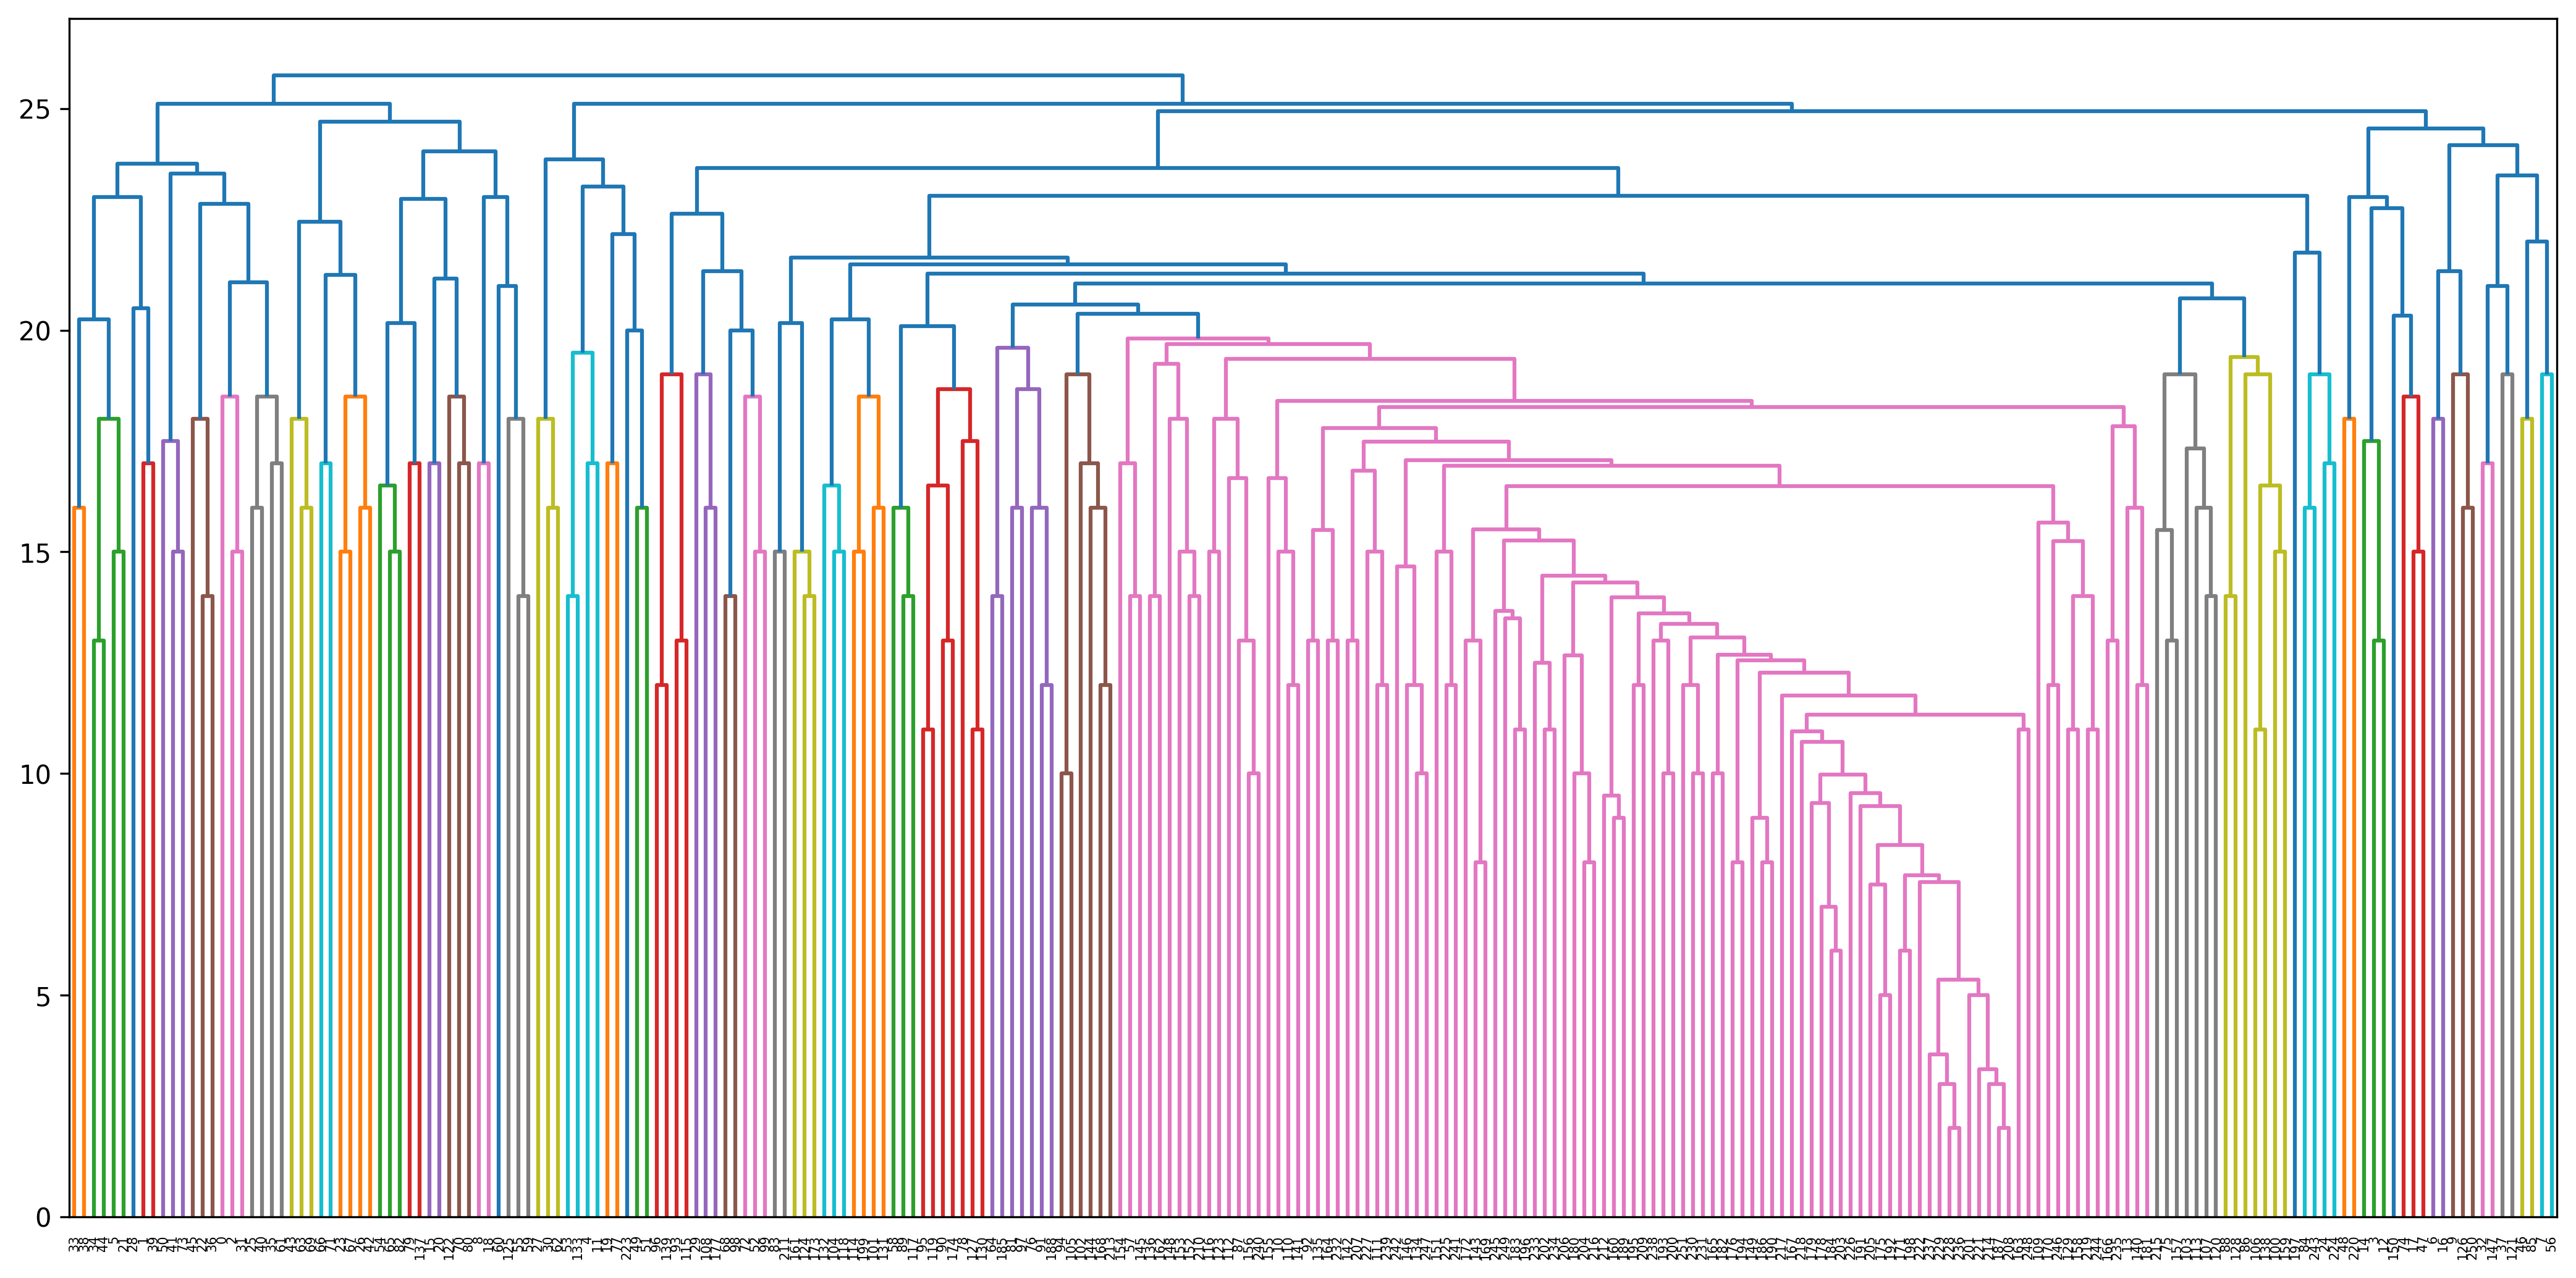
\includegraphics[width=\linewidth]{../Quantum-Annealing-for-solving-QUBO-Problems/test/Diagnostica_QALS/2/Decay_factor/ksp_2/lambda_div_3/dendrogram_2000_1.png}
\caption{Agglomerative Clustering Dendogram}
\label{fig:AgglomerativeClustering-ksp2}
\end{figure}

\subsection{Riassunto dati}
\begin{table}[h]
\centering
\begin{tabular}{lccc|ccc}
\hline
& \multicolumn{3}{c|}{\(\boldsymbol{\lambda_1}\)}
& \multicolumn{3}{c}{\(\boldsymbol{\lambda_2}\)} \\
\cline{2-7}

\textbf{Istanza}
& \(\boldsymbol{f_Q}\)
& \(\boldsymbol{N_{\mathrm{cluster}}}\)
& \(\boldsymbol{|C_{\max}|}\)
& \(\boldsymbol{f_Q}\)
& \(\boldsymbol{N_{\mathrm{cluster}}}\)
& \(\boldsymbol{|C_{\max}|}\) \\
\hline

\texttt{ksp\_1}
& -267.3
& 8
& 225
& -1454230.67
& 13
& 140 \\

\texttt{ksp\_3}
& 31096.64
& 34
& 74
& 6043281857.67
& 36
& 89 \\

\texttt{ksp\_2}
& 2232153.7
& 49
& 102
& 417407498726.0
& 0
& 105 \\

\hline
\end{tabular}

\caption{Confronto del valore obiettivo e delle caratteristiche del
clustering utilizzando \(\lambda_1\) e \(\lambda_2\).}
\label{tab:clustering-lambda-confronto}
\end{table}

\subsection{Interpretazione dei risultati con Decay Factor}
L' introduzione del decay factor nella matrice tabù ha lo scopo di ridurre progressivamente il contributo delle penalizzazioni associate alle soluzioni visitate
nelle iterazioni precedenti. In questo modo, le informazioni più recenti mantengono un peso maggiore, mentre quelle più vecchie vengono gradualmente dimenticate. 
L' obiettivo è evitare che l' accumulo delle penalizzazioni nella matrice S condizioni eccessivamente la ricerca nelle fasi avanzate dell' algoritmo.

L' interpretazione di:
\[
d_H(z_{\text{starOld}}, z_{\text{starNew}})
\qquad
d_H(z_{\text{opt}}, z_{\text{star}})
\qquad
f_Q(z_{\text{star}})
\]
rimane la medesima. \(z_{\text{opt}}\) cambia raramente ma sempre a diminuire. Ad accezione del test case
\texttt{ksp\_2} con \(\lambda_1\) che presenta un numero di cambiamenti maggiore rispetto agli altri test case.

Sono simili anche i risultati di:
\[
d_H(z_t, z_{\text{star}})
\qquad
d_H(z_{\text{opt}}, z_t)
\qquad 
Numero Cluster.
\]
Cambiano però:
\begin{itemize}
    \item dimensioni dei cluster, risultano essere più omogenee il che permette di far pensare ad un' esplorazione migliore rispetto al non usare il decay factor;
    \item \(f_Q(z_t)\) la quale tende a decrescere, specialmente nei casi in cui si utilizza \(\lambda_1\).
\end{itemize}

\end{document}
